%%%==========Nội dung file thứ 1===============%%%

\dongkeex
\dongkebt
\section{Các thành phần của nguyên tử}
\begin{Muctieu}
	\begin{itemize}
		\item Trình bày được thành phần của nguyên tử.
		\item So sánh được khối lượng của electron với proton và nơtron
		\item So sánh được kích thước của hạt nhân với nguyên tử
	\end{itemize}
\end{Muctieu}
\subsection{NỘI DUNG BÀI HỌC}
\subsubsection{SỰ PHÁT TRIỂN MÔ HÌNH NGUYÊN TỬ}
\begin{tomtat}
	\begin{minipage}[htp!]{0.5\textwidth}
		Từ thời cổ Hy Lạp,nhà triết học Democritous (Đê-mô-crít) (Hình \ref{fig:Democritus})
		Mọi thứ trên thế giới đều được tạo ra từ các hạt nhỏ không thể chia nhỏ được nữa được gọi là \textbf{“nguyên tử”}, có nghĩa là \textbf{“không thể thay đổi được”}
	\end{minipage}
	\begin{minipage}[htp!]{0.5\textwidth}
		\begin{center}
			\includegraphics[width=3cm]{Images/anhhoahoc10/DEMOCRITUS.png}
			\captionof{figure}{Democritus (460 - 370,Hy Lạp)\label{fig:Democritus} }
		\end{center}
	\end{minipage}
	
	\begin{center}
		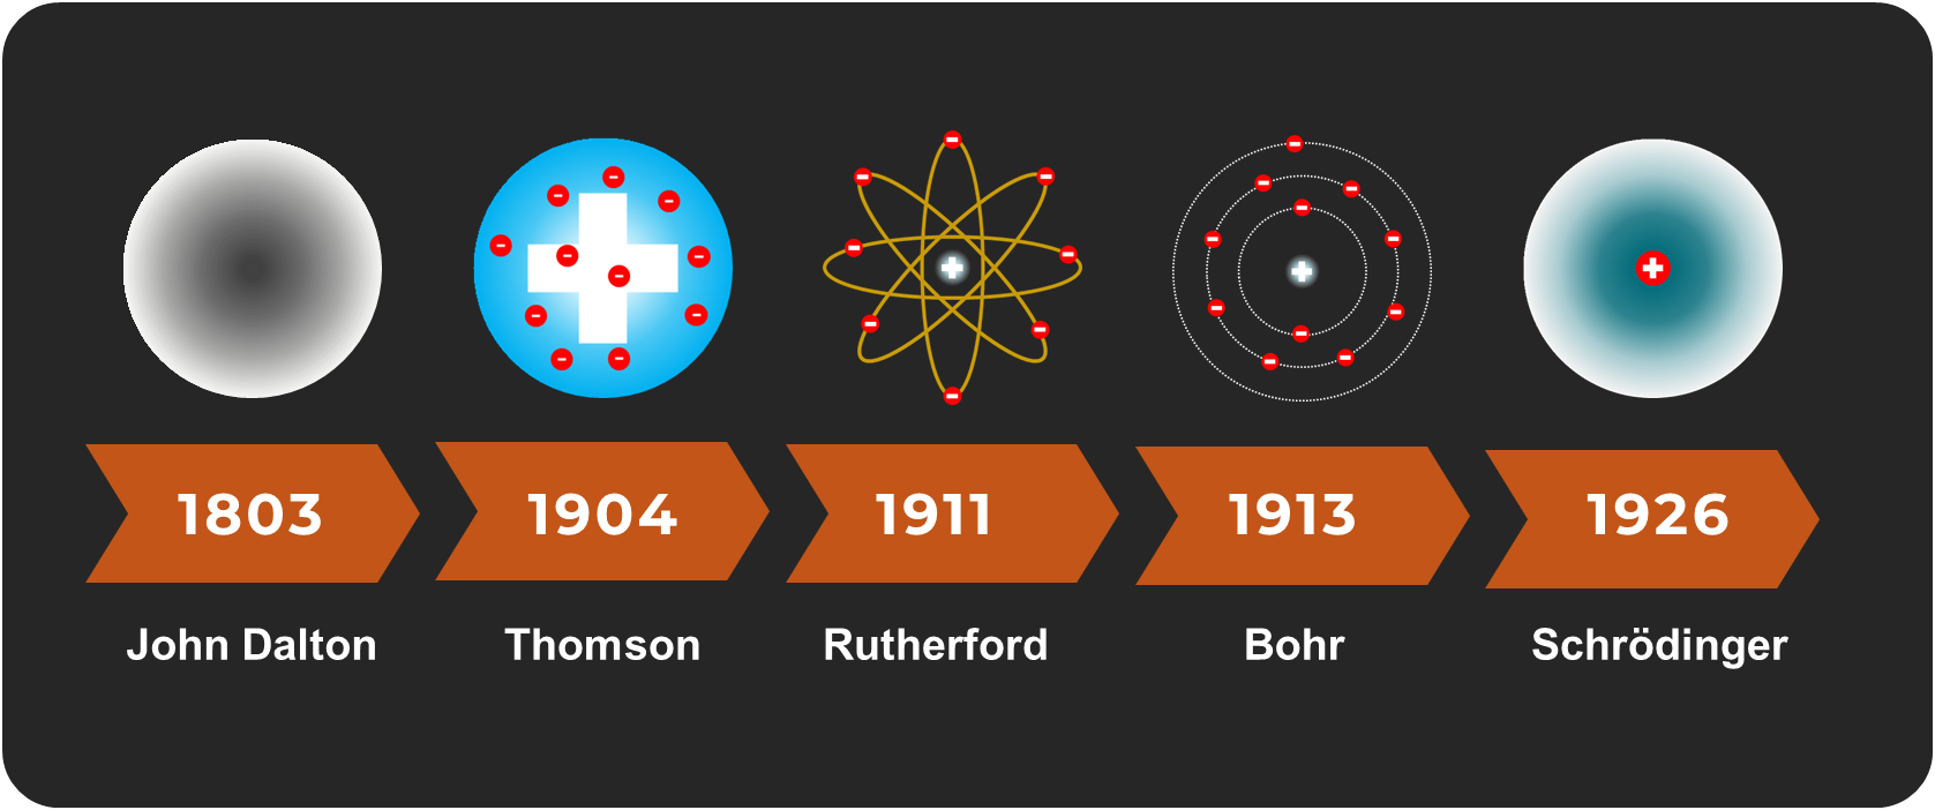
\includegraphics[width=12cm]{Images/anhhoahoc10/historyatom.png}
		\captionof{figure}{Lịch sử phát triển mô hình nguyên tử \label{fig:Historyatom} }
	\end{center}
\end{tomtat}
\subsubsection{Thành phần và cấu trúc của nguyên tử}
\Noibat[][][\faArrowCircleOLeft]{Thành phần}
\vspace{0.5cm}
\begin{tomtat}
	Nguyên tử gồm hạt nhân chứa proton, neutron và vỏ nguyên tử chứa electron.
	\begin{center}
		\includegraphics[width=9cm]{Images/anhhoahoc10/mohinhnguyentu.png}
		\captionof{figure}{Mô hình nguyên tử}
	\end{center}
\end{tomtat}
\subsubsection{Sự tìm ra electron}
\Noibat[][][\faArrowCircleOLeft]{Thí nghiệm khám phá tia âm cực của Thomson}\\
Năm 1897, J. J. Thomson (Tôm-xơn, người Anh) thực hiện thí nghiệm phóng điện qua không khí loãng đã phát hiện ra chùm tia phát ra từ cực âm.(xem hình \ref{fig:hinh3} ) và link video bằng mã QR ở bên dưới.\\ 
\hinhphai{\begin{center}
		\includegraphics[width=9cm]{Images/anhhoahoc10/TNTHOMSON.png}\\
		\captionof{figure}{Thí nghiệm của Thomson}
		\label{fig:hinh3}
\end{center}}{\begin{tikzpicture}
		\path (0,0)  node (QRCODE) {\maqr[\maunhan][3]{https://youtu.be/y2uswXtC5O8}}
		(QRCODE.south) node[anchor=north]{(\fmmfamily Các bạn  dùng ~\rotatebox{-15}{\faMobile}~quét mã QR để xem video TN nhé!)}
		;
\end{tikzpicture}}

\begin{hoivadap}
	\begin{cauhoi}
		Vai trò của lớp bột huỳnh quang trong thí nghiệm ở hình \ref{fig:hinh3}
	\end{cauhoi}
	\loigiai{\taodongke{3}}
\end{hoivadap}

\begin{hoivadap}
	\begin{cauhoi}
		Quan sát Hình \ref{fig:hinh3} và video , giải thích vì sao tia âm cực bị hút về cực dương của trường điện.
	\end{cauhoi}
	\loigiai{\taodongke{3}}
\end{hoivadap}
%
\begin{hoivadap}
	\begin{cauhoi}
		Nếu đặt một chong chóng nhẹ trên đường đi của tia âm cực thì chong chóng sẽ quay. Từ hiện tượng đó, hãy nêu kết luận về tính chất của tia âm cực.
	\end{cauhoi}
	\loigiai{\taodongke{3}}
\end{hoivadap}

\begin{Bancobiet}
	Mô hình Thomson còn gọi là mô hình \lq\lq bánh pudding mận".Theo Thomson:
	\begin{enumerate}
		\item Nguyên tử là quả cầu mang điện tích dương, bên trong chứa các êlectron.
		\item Nguyên tử trung hòa về điện.
	\end{enumerate}
\end{Bancobiet}
%
%
\subsubsection{Sự khám phá hạt nhân nguyên tử}
\Noibat[][][\faArrowCircleOLeft]{Tìm hiểu thí nghiệm của Rutherford}\\
Năm 1911, E. Rutherford (Ro-dơ-pho, người Niu Di-lân) thực hiện thí nghiệm bắn phá lá vàng rất mỏng bằng chùm hạt $ \alpha $ \footnote{Hạt $\alpha$ : hạt nhân helium, mang điện tích dương.} (xem hình \ref{fig:hinh4})
\begin{center}
	\includegraphics[width=9cm]{Images/anhhoahoc10/TNRUTHERFORT.png}\\
	\captionof{figure}{Thí nghiệm của Rutherford}
	\label{fig:hinh4}
\end{center}

\begin{center}
	\includegraphics[width=9cm]{Images/anhhoahoc10/KQTN.png}\\
	\captionof{figure}{Kết quả thí nghiệm của Rutherford}
	\label{fig:hinh5}
\end{center}
%
\begin{hoivadap}
	\begin{cauhoi}
		Quan sát hình \ref{fig:hinh4}, cho biết các hạt $\alpha$ có đường đi như thế nào. Dựa vào Hình \ref{fig:hinh5} , giải thich kết quả thí nghiệm thu được.
	\end{cauhoi}
	\loigiai{\taodongke{5}}
\end{hoivadap}
%\vspace*{6pt}
\begin{tomtat}
	{\bfseries{Kết luận}}
	\begin{itemize}
		\item Nguyên tử có cấu tạo rỗng, gồm hạt nhân ở trung tâm và lớp vỏ là các electron chuyển động xung quanh hạt nhân.
		\item Nguyên tử trung hoà về điện: số đơn vị điện tích dương của hạt nhân bằng số đơn vị điện tích âm của các electron trong nguyên tử.
	\end{itemize}
\end{tomtat}
\subsubsection{Cấu tạo hạt nhân nguyên tử}
\begin{center}
	\includegraphics[width=9cm]{Images/anhhoahoc10/CAUTAOHATNHAN.png}\\
	\captionof{figure}{Thành phần của hạt nhân}
	\label{fig:hinh6}
\end{center}
\begin{hoivadap}
	\begin{cauhoi}
		Quan sát hình \ref{fig:hinh6} và kết hợp SGK , các bạn hãy nêu thành phần của hạt nhân
	\end{cauhoi}
\end{hoivadap}
\begin{ghinho}
	Proton, neutron và electron là các hạt cấu tạo nên nguyên tử.
\end{ghinho}
\begin{tongket}{Tổng kết}
	Thành phần cấu tạo của nguyên tử gồm:
	\begin{itemize}
		\item  Hạt nhân (nucleus): ở tâm của nguyên tử, chứa các proton mang điện tích dương và các neutron không mang điện.
		\item Vỏ nguyên tử: chứa các electron mang điện tích âm, chuyển động rất nhanh xung quanh hạt nhân.
		\item Trong nguyên tử, số proton bằng số electron nên nguyên tử trung hoà điện.
		\item Khối lượng của electron rất nhỏ, không đáng kể so với khối lượng của proton hay neutron nên khối lượng của nguyên tử tập trung hầu hết ở hạt nhân.
	\end{itemize}
\end{tongket}
%
%
\begin{longtable}{|c|c|c|c|c|c|}
	\caption{\indam[\maunhan]{Khối lượng, điện tích của các loại hạt cấu tạo nên nguyên tử}}
	\label{tab:ktntklnt}\\
	\hline
	\rowcolor{\mauphu!25} \indam[\mauphu]{Hạt} & \indam[\mauphu]{Kí hiệu} & $\begin{array}{c}\text {\indam[\mauphu]{Khối lượng} } \\
		\text {\indam[\mauphu]{(kg)}  }\end{array}$ & \indam[\mauphu]{Khối lượng (amu)} & $\begin{array}{c}\text { \indam[\mauphu]{Điện tích} } \\
		\text { \indam[\mauphu]{(C)} }\end{array}$ & $\begin{array}{l}\text { \indam[\mauphu]{Điện tích} } \\
		\text { \indam[\mauphu]{tương đối} }\end{array}$ \\
	\hline\endhead
	\rowcolor{\mycolor!15} Proton & $p$ & $1,672 \cdot 10^{-27}$ & $\approx 1$ & $1,602 \cdot 10^{-19}$ & +1 \\
	\hline
	\rowcolor{\mycolor!15} Neutron & $\mathrm{n}$ & $1,675 \cdot 10^{-27}$ & $\approx 1$ & 0 & 0 \\
	\hline\rowcolor{\mycolor!15} Electron & e & $9,109 \cdot 10^{-31}$ & $\begin{array}{c}
		~ \\
		\dfrac{1}{1837} \approx 0,00055\\
		~ \\
	\end{array}$ & $-1,602 \cdot 10^{-19}$ & -1 \\
	\hline
\end{longtable}
\subsubsection{Kích thước và khối lượng nguyên tử}
\begin{center}
	\includegraphics[width=9cm]{Images/anhhoahoc10/ktnt.png}\\
	\captionof{figure}{So sánh kích thước hạt nhân , nguyên tử}
	\label{fig:m-q-hatcoban}
\end{center}
\vspace*{0.25cm}
\begin{note}
	\begin{itemize}
		\item Đơn vị kích thước thường dùng của nguyên tử là Angstron ($ A^0 $) hoặc nano mét (nm)			
		$$1 \mathrm{~nm}=10^{-9}~\mathrm{m} ; 1 A^0=10^{-10}~\mathrm{~m} ; 1 \mathrm{~nm}=10 A^0; 1 A^0=10^{2}~\mathrm{pm}$$
		\begin{center}
			\tcbox[width=5cm,colframe=\maunhan]{$ \dfrac{d_{\text{NT}}}{d_{\text{hạt nhân}}}\approx \dfrac{10^{-10}}{10^{-14}} \approx 10^4~\mathrm{\text{lần}} $}
		\end{center}
		\item Đơn vị của khối lương nguyên tử là amu (atomic mass unit),
		$$
		1 \mathrm{amu}=1,6605 \times 10^{-27} \mathrm{~kg} \text {. }
		$$
		\item Đơn vi của điện tích các hạt cơ bản là $\mathrm{e}_0$ (điện tích nguyên tố),
		$$
		1 \mathrm{e}_0=1,602 \times 10^{-19} \mathrm{C} \text {. }
		$$
	\end{itemize}
\end{note}
\newpage
\subsection{Các dạng bài tập}
\begin{dang}{Lý thuyết về cấu tạo nguyên tử}
	\Noibat[][][\faCamera]{Phương pháp giải}
	\begin{itemize}
		\item Nắm vững về cấu tạo nguyên tử
		\item Nắm vững kết quả thí nghiệm của Thomson,Rutherford
	\end{itemize}
\end{dang}
\Noibat[\maunhan][][\faBookmark]{Ví dụ mẫu}
%%%%============VDEX1==============%%%
\begin{vdex}
	Các hạt cơ bản của hầu hết các nguyên tử là?
	\choice
	{electron}
	{electron và proton}
	{proton và notron}
	{\True electron, proton và notron}
	\loigiai{}
\end{vdex}
%%%%============VDEX2==============%%%
\begin{vdex}
	Hạt nhân của hầu hết các nguyên tử gồm có?
	\choice
	{electron}
	{electron và proton}
	{\True proton và notron}
	{electron, proton và notron}
	\loigiai{}
\end{vdex}
%%%%============VDEX3==============%%%
\begin{vdex}
	Trong thí nghiệm của Thomson, phát biểu nào sau đây sai với kết quả thí nghiệm ta quan sát được?
	\choice
	{Tia âm cực là các chùm hạt electron di chuyển từ cực âm sang cực dương}
	{Tia âm cực là chùm hạt mang điện tích âm}
	{\True	Tia âm cực bị lệch về phía bản cực âm của nguồn điện}
	{Tia âm cực bị lệch hướng khi ta đặt nó trong từ trường}
	\loigiai{}
\end{vdex}

%%%%============Bài tập tự luyện dạng 1==============%%%
\Noibat[][][\faBank]{Bài tập tự luyện dạng \thedang}
%%%=========Câu hỏi trắc nghiệm 1 phương án=========%%%
\phan{Câu hỏi trắc nghiệm 1 phương án}
\Opensolutionfile{ansex}[Ans/LGEX-Hoa10_C01B01_CTNT_BTTL01]
\Opensolutionfile{ans}[Ans/Ans-Hoa10_C01B01_CTNT_BTTL01]
%\hienthiloigiaiex
%\tatloigiaiex
%\luuloigiaiex
%%%=============EX_1=============%%%
\begin{ex}
	Hạt mang điện dương trong hạt nhân nguyên tử là
	\choice
	{Electron}
	{\True Proton}
	{Neutron}
	{Photon}
	\loigiai{
		Proton là hạt mang điện dương trong hạt nhân nguyên tử. Electron mang điện âm, neutron không mang điện.
	}
\end{ex}

%%%=============EX_2=============%%%
\begin{ex}
	Số proton trong hạt nhân nguyên tử được gọi là
	\choice
	{Số khối}
	{Số neutron}
	{\True Số hiệu nguyên tử}
	{Số electron}
	\loigiai{
		Số hiệu nguyên tử (kí hiệu Z) chính là số proton trong hạt nhân nguyên tử. Nó xác định danh tính của nguyên tố hóa học.
	}
\end{ex}

%%%=============EX_3=============%%%
\begin{ex}
	Nguyên tử trung hòa về điện có số
	\choice
	{Proton lớn hơn số electron}
	{Electron lớn hơn số proton}
	{\True Proton bằng số electron}
	{Neutron bằng số proton}
	\loigiai{
		Trong nguyên tử trung hòa về điện, số proton (mang điện dương) bằng số electron (mang điện âm), do đó tổng điện tích bằng 0.
	}
\end{ex}

%%%=============EX_4=============%%%
\begin{ex}
	Số khối A của một nguyên tử được tính bằng
	\choice
	{Số proton - số neutron}
	{Số electron + số neutron}
	{\True Số proton + số neutron}
	{Số proton + số electron}
	\loigiai{
		Số khối A = số proton + số neutron. Đây là tổng số hạt trong hạt nhân nguyên tử.
	}
\end{ex}

%%%=============EX_5=============%%%
\begin{ex}
	Nguyên tử ${^{23}_{11}Na}$ có bao nhiêu neutron?
	\choice
	{11}
	{\True 12}
	{23}
	{34}
	\loigiai{
		Trong ${^{23}_{11}Na}$, số khối $A = 23$, số hiệu nguyên tử $Z = 11$.
		Số neutron $= A - Z = 23 - 11 = 12$
	}
\end{ex}

%%%=============EX_6=============%%%
\begin{ex}
	Đồng vị là các nguyên tử có cùng
	\choice
	{Số khối}
	{Số neutron}
	{\True Số proton}
	{Số electron}
	\loigiai{
		Đồng vị là các nguyên tử có cùng số proton (số nguyên tử) nhưng khác nhau về số neutron (và do đó khác nhau về số khối).
	}
\end{ex}

%%%=============EX_7=============%%%
\begin{ex}
	Hạt nào sau đây không có trong hạt nhân nguyên tử?
	\choice
	{Proton}
	{Neutron}
	{\True Electron}
	{Proton và neutron}
	\loigiai{
		Hạt nhân nguyên tử chỉ chứa proton và neutron. Electron quay xung quanh hạt nhân trong lớp vỏ nguyên tử.
	}
\end{ex}

%%%=============EX_8=============%%%
\begin{ex}
	Trong một nguyên tử, nếu số proton là 8 và số neutron là 9, số khối của nguyên tử đó là bao nhiêu?
	\choice
	{8}
	{9}
	{16}
	{\True 17}
	\loigiai{
		Số khối $A = \text{số proton} + \text{số neutron}$
		Trong trường hợp này: $A = 8 + 9 = 17$
	}
\end{ex}

%%%=============EX_9=============%%%
\begin{ex}
	Đơn vị nào thường được sử dụng để đo kích thước của nguyên tử?
	\choice
	{Milimet ($mm$)}
	{\True Picomet ($pm$)}
	{decimet ($dm$)}
	{centimet ($cm$)}
	\loigiai{
		Kích thước nguyên tử thường được đo bằng đơn vị picomet (pm). $1 pm = 10^-12 m$, phù hợp với kích thước cực nhỏ của nguyên tử.
	}
\end{ex}

%%%=============EX_10=============%%%
\begin{ex}
	Hạt nào sau đây có khối lượng gần bằng khối lượng của proton?
	\choice
	{Electron}
	{\True Neutron}
	{Positron}
	{Alpha}
	\loigiai{
		Neutron có khối lượng gần bằng khối lượng của proton. Electron có khối lượng rất nhỏ so với proton. Positron là phản hạt của electron. Hạt alpha là hạt gồm 2 proton và 2 neutron.
	}
\end{ex}
%%%=============EX_11=============%%%
\begin{ex}
	Theo mô hình bánh pudding mận của Thomson, phát biểu nào sau đây là đúng?
	\choice
	{%
		Nguyên tử có cấu tạo rỗng gồm hạt nhân mang điện tích dương và vỏ là các electron chuyển động xung quanh hạt nhân.
	}
	{%
		Nguyên tử có cấu tạo rỗng gồm hạt nhân mang điện tích dương và vỏ là các electron chuyển dộng xung quanh hạt nhân theo những quỹ đạo có kích thước và năng lượng cố định
	}
	{%
		\True	nguyên tử bao gồm các electron nằm rải rác trong một đám mây hình cầu mang điện tích dương.
	}
	{%
		các electron  quay quanh hạt nhân không theo một quỹ đạo xác định, mà chúng tạo thành các đám mây điện tích mà tại đó xác suất tìm thấy electron là lớn nhất
	}
	\loigiai{
		Theo mô hình bánh pudding mận của Thomson nguyên tử bao gồm các electron nằm rải rác trong một đám mây hình cầu mang điện tích dương
	}
\end{ex}

%%%=============EX_12=============%%%
\begin{ex}
	Cho các phát biểu sau:
	\begin{enumerate}[(1)]
		\item Tất cả các hạt nhân nguyên tử đều được cấu tạo từ các hạt proton và neutron.
		\item Khối lượng nguyên tử tập trung phần lớn ở lớp vỏ.
		\item Trong nguyên tử, số electron bằng số proton.
		\item Trong hạt nhân nguyên tử, hạt mang điện là proton và electron.
		\item Trong nguyên tử, hạt electron có khối lượng không đáng kể so với các hạt còn lại.
	\end{enumerate}
	Số phát biểu đúng là
	\choice
	{%
		1
	}
	{%
		\True 2
	}
	{%
		3
	}
	{%
		4
	}
	\loigiai{%
		Phát biểu đúng là:
		Trong hạt nhân nguyên tử, hạt mang điện là proton và electron.\\
		Trong nguyên tử, hạt electron có khối lượng không đáng kể so với các hạt còn lại
	}
\end{ex}

%%%=============EX_13=============%%%
\begin{ex}
	Điều nào sau đây đúng theo mô hình nguyên tử của Thomson?
	\choice
	{%
		Nguyên tử không trung hòa về điện
	}
	{%
		\True Nguyên tử là quả cầu mang điện tích dương có chứa các electron bên trong
	}
	{%
		Điện tích âm và điện tích dương trong nguyên tử có độ lớn bằng nhau
	}
	{%
		Không có điều nào ở trên
	}
	\loigiai{
		Nguyên tử là quả cầu mang điện tích dương có chứa các electron bên trong
	}
\end{ex}

%%%=============EX_14=============%%%
\begin{ex}
	Trong hiện tượng xả điện qua khí ở áp suất thấp, sự tỏa sáng màu trong ống xuất hiện là kết quả của:
	\choice
	{%
		\True va chạm giữa các hạt mang điện được phát ra từ cực âm và nguyên tử của khí
	}
	{%
		va chạm giữa các electron khác nhau của các nguyên tử trong khí
	}
	{%
		kích thích các electron trong các nguyên tử
	}
	{%
		va chạm giữa các nguyên tử của khí
	}
	\loigiai{
		sự tỏa sáng màu trong ống xuất hiện là kết quả của va chạm giữa các hạt mang điện được phát ra từ cực âm và nguyên tử của khí
	}
\end{ex}

%%%=============EX_15=============%%%
\begin{ex}
	Mô hình đầu tiên về nguyên tử được đưa ra bởi:
	\choice
	{%
		N. Bohr
	}
	{%
		E. Goldstein
	}
	{%
		Rutherford
	}
	{%
		\True J.J. Thomson
	}
	\loigiai{
		Mô hình nguyên tử đầu tiên được đưa ra bởi JJ Thomson. Theo ông, nguyên tử bao gồm một quả cầu mang điện tích dương với các electron mang điện tích âm được nhúng trong đó.
	}
\end{ex}

%%%=============EX_16=============%%%
\begin{ex}
	Nếu đường kính của nguyên tử khoảng $10^2 \mathrm{pm}$ thì đường kính của hạt nhân khoảng
	\choice
	{%
		$10^2 \mathrm{pm}$
	}
	{%
		$10^{-4} \mathrm{pm}$
	}
	{%
		\True	$10^{-2} \mathrm{pm}$
	}
	{
		$10^4 \mathrm{pm}$
	}
	\loigiai{
		Ta có $\dfrac{d_{NT}}{d_{\text{hạt nhân}}} =10^4$ (lần)
		$\Rightarrow d_{\text{hạt nhân}} = \dfrac{d_{NT}}{10^4}=\dfrac{10^2}{10^4}=10^{-2}$ (pm)
	}
\end{ex}
\Closesolutionfile{ans}
\Closesolutionfile{ansex}
%\bangdapan{Ans-Hoa10_C01B01_CTNT_BTTL01}

%%%===========Bài tập tự luyện dạng tự luận dạng 1=============%%%%
\phan{BÀI TẬP TỰ LUẬN}
\Opensolutionfile{ansbth}[Ans/LGBT-Hoa10_C01B01_CTNT_BTTL01]
\Opensolutionfile{ansbt}[Ans/AnsBT-Hoa10_C01B01_CTNT_BTTL01]
%\luuloigiaibt
%%%=============BT_1=============%%%
\begin{bt}
	Trong thí nghiệm của Rutherford, khi sử dụng các hạt alpha (ion $\mathrm{He}^{2+}$, kí hiệu là $\mathrm{a}$ ) bắn vào lá vàng thì:
	\begin{itemize}
		\item Hầu hết các hạt a xuyên thẳng qua lá vàng.
		\item Một số ít hạt a bị lệch quỹ đạo so với ban đầu.
		\item Một số rất ít hạt a bị bật ngược trở lại.
	\end{itemize}
	Từ kết quả này, em có nhận xét gì về cấu tạo nguyên tử?
	\loigiai{
		Trong thí nghiệm của Rutherford, khi sử dụng các hạt alpha (ion $\mathrm{He}^{2+}$, kí hiệu là a) bắn vào lá vàng thì:
		\begin{itemize}
			\item Hầu hết các hạt a xuyên thẳng qua lá vàng chứng tỏ nguyên tử có cấu tạo rỗng.
			\item Một số ít hạt a bị lệch quỹ đạo so với ban đầu chứng tỏ hạt nhân nguyên tử cùng điện tích dương như hạt hạt alpha (ion $\mathrm{He}^{2+}$, kí hiệu là $ \alpha $).
			\item Một số rất ít hạt a bị bật ngược trở lại chứng tỏ kích thước hạt nhân nhỏ hơn rất nhiều so với kích thước của nguyên tử và khối lượng nguyên tử tập trung chủ yếu ở hạt nhân.
		\end{itemize}
	}
\end{bt}
%%%=============BT_2=============%%%
\begin{bt}
	Viết lại bảng sau vào vở và điền thông tin còn thiếu vào các ô trống:\par\noindent
		\begin{longtable}{|c|c|c|c|c|c|c|}
			\hline \indam{Nguyên tố} & \indam{Kí hiệu} &  \indam{Z} & \indam{Số e} & \indam{Số p} & \indam{Số n} & \indam{Số khối} \\
			\endfirsthead
			\hline \indam{Nguyên tố} & \indam{Kí hiệu} &  \indam{Z} & \indam{Số e} & \indam{Số p} & \indam{Số n} & \indam{Số khối} \\
			\endhead
			\hline \indam{Carbon} & $\mathrm{C}$ & 6 & 6 & $?$ & 6 & $?$ \\
			\hline \indam{Nitrogen} & $\mathrm{N}$ & 7 & $?$ & 7 & $?$ & 14 \\
			\hline \indam{Oxygen} & $\mathrm{O}$ & 8 & 8 & $?$ & 8 & $?$ \\
			\hline \indam{Sodium (natri)} & $\mathrm{Na}$ & 11 & $?$ & 11 & $?$ & 23 \\
			\hline \indam{Aluminium (nhôm)} & $\mathrm{Al}$ & $?$ & 13 & $?$ & $?$ & 27 \\
			\hline
		\end{longtable}
	\loigiai{%
		\begin{longtable}{|c|c|c|c|c|c|c|}
			\hline\rowcolor{\mycolor!10}
			\indam{Nguyên tố} & \indam{Kí hiệu} &  \indam{Z} & \indam{Số e} & \indam{Số p} & \indam{Số n} & \indam{Số khối} \\
			\hline 
			\endfirsthead
			\hline\rowcolor{\mycolor!10}
			\indam{Nguyên tố} & \indam{Kí hiệu} &  {$\mathbf{Z}$} & \indam{Số e} & \indam{Số p} & \indam{Số n} & \indam{Số khối} \\
			\hline \endhead
			\hline\endfoot
			\indam{Carbon} & $\mathrm{C}$ & 6 & 6 & 6 & 6 & 12 \\
			\hline 
			\indam{Nitrogen} & $\mathrm{N}$ & 7 & 7 & 7 & 7 & 14 \\
			\hline 
			\indam{Oxygen} & $\mathrm{O}$ & 8 & 8 & 8 & 8 & 16 \\
			\hline 
			\indam{Sodium (natri)} & $\mathrm{Na}$ & 11 & 11 & 11 & 12 & 23\\
			\hline 
			\indam{Aluminium (nhôm)} & $\mathrm{Al}$ & 13 & 13 & 13 & 14 &27\\
			\hline
		\end{longtable}
	}
\end{bt}
%%%=============BT_3=============%%%
\begin{bt}
	Nối tên các nhà khoa học ở cột A với những đóng góp của họ trong việc tìm hiểu cấu trúc nguyên tử ở cột B
	\par\noindent
		\begin{longtable}{|p{0.3\linewidth}|p{0.4\linewidth}|}
			% Nội dung cho đầu trang đầu tiên
			\hline\rowcolor{\mycolor!10}
			Cột A & Cột B \\
			\hline
			\endfirsthead
			% Nội dung cho đầu các trang tiếp theo
			\hline\rowcolor{\mycolor!10}
			Cột A & Cột B \\
			\hline
			\endhead
			% Nội dung cho chân trang (trừ trang cuối)
			\hline
			\endfoot
			% Nội dung cho chân trang cuối cùng
			\hline
			\endlastfoot
			% Nội dung chính của bảng bắt đầu từ đây
			(a) Ernest Rutherford & (i) Tính không thể phân chia của nguyên tử\\
			(b) J.J.Thomson &(ii) Các quỹ đạo dừng\\
			(c) Dalton &(iii) Khái niệm hạt nhân\\
			(d) Neils Bohr &(iv) Phát hiện electron\\
			(e) James Chadwick &(v) Số nguyên tử\\
			(f) E. Goldstein &(vi) Nơtron\\
			(g) Mosley &(vii) Tia âm cực\\
			\hline
		\end{longtable}
	\loigiai{%
		\noindent
		(a) Ernest Rutherford -- (iii) Khái niệm hạt nhân\\
		(b) J.J.Thomson -- (iv) Phát hiện electron\\
		(c) Dalton -- (i) Tính không thể phân chia của nguyên tử\\
		(d) Neils Bohr -- (ii) Các quỹ đạo dừng\\
		(e) James Chadwick -- (vi) Nơtron\\
		(f) E. Goldstein -- (vii) Tia âm cực\\
		(g) Mosley -- (v) Số nguyên tử
	}
\end{bt}
%%%==============BT4==============%%%
\begin{bt}
	Một loại nguyên tử nitrogen có 7 proton và 7 neutron trong hạt nhân. Dựa vào Bảng \ref{tab:ktntklnt}, hãy tính và so sánh:
	\begin{enumerate}
		\item Khối lượng hạt nhân với khối lượng nguyên tử.
		\item Khối lượng hạt nhân với khối lượng vỏ nguyên tử.
	\end{enumerate}
	\loigiai{Từ bảng \ref{tab:ktntklnt}, ta có:\\
			$m(\text{proton}) = m(\text{neutron}) \approx 1,67 \cdot 10^{-27} \text{ kg} $, $m(\text{electron}) = 9,109 \cdot 10^{-31} \text{ kg}$
			\\
		Nguyên tử nitrogen có 7 proton, 7 neutron và 7 electron (vì là nguyên tử trung hòa).
		
		\begin{enumerate}
			\item So sánh khối lượng hạt nhân với khối lượng nguyên tử:
			\begin{align*}
				\text{Khối lượng hạt nhân} &= 7m(\text{proton}) + 7m(\text{neutron}) \\
				&= 7 \cdot 1,67 \cdot 10^{-27} + 7 \cdot 1,67 \cdot 10^{-27} \\
				&= 23,38 \cdot 10^{-27} \text{ kg}
			\end{align*}
			\begin{align*}
				\text{Khối lượng nguyên tử} &= \text{khối lượng hạt nhân} + \text{khối lượng 7 electron} \\
				&= 23,38 \cdot 10^{-27} + 7 \cdot 9,109 \cdot 10^{-31} \\
				&= 23,38 \cdot 10^{-27} + 0,064 \cdot 10^{-27} \\
				&= 23,444 \cdot 10^{-27} \text{ kg}
			\end{align*}
			
			Ta thấy khối lượng hạt nhân chiếm 99,73\% khối lượng nguyên tử.
			\item So sánh khối lượng hạt nhân với khối lượng vỏ nguyên tử:
			\begin{align*}
				\text{Khối lượng vỏ nguyên tử} &= \text{khối lượng 7 electron} \\
				&= 7 \cdot 9,109 \cdot 10^{-31} = 0,064 \cdot 10^{-27} \text{ kg}
			\end{align*}
			\begin{align*}
			\text{Tỉ lệ khối lượng hạt nhân} : \text{khối lượng vỏ}	&= 23,38 \cdot 10^{-27} : 0,064 \cdot 10^{-27} \\
				&\approx 365{,}3 : 1
			\end{align*}
			Vậy khối lượng hạt nhân gấp khoảng $365{,}3$ lần khối lượng vỏ nguyên tử.
		\end{enumerate}
	}
\end{bt}

\Closesolutionfile{ansbt}
\Opensolutionfile{ansbth}

%%%%%====================Dạng 2=====================%%%
\newpage
\begin{dang}{Bài tập về khối lượng, kích thước nguyên tử}	
	\Noibat[][][\faCamera]{Phương pháp giải}
	\tieumuc{Các công thức liên quan khối lượng}
	\begin{itemize}
		\item $ m _{\text{nguyên tử}=m_{p}+m_{n} + m_{e} } $ (tính chính xác); $ m _{\text{nguyên tử}} \approx  m_{p} + m_{n} \approx m_{\text{hạt nhân}} $ (tính gần đúng)
		\item Khối lượng tính ra kg của 1 nguyên tử carbon-12 là $ 19,926 . 10^{27}~\mathrm{kg}$.
		\item 1 amu được định nghĩa bằng $\dfrac{1}{12}$ khối lượng 1 nguyên tử carbon-12:
		\item$1 \mathrm{amu}=\dfrac{19,926 \cdot 10^{-27} \mathrm{~kg}}{12}=1,661 \cdot 10^{-27} \mathrm{~kg}$
		\item$1 \mathrm{mol}$ chứa $ 6,02.10^{23} $ nguyên tử, phân tử, ion.
	\end{itemize}
	\tieumuc{Các công thức liên quan kích thước}
	\begin{itemize}
		\item Thể tích của hình cầu:
		$ V=\dfrac{4}{3}\pi r^3 $
		\item Phần trăm thể tích các nguyên tử trong tinh thể $ = \dfrac{V_{\text{các nguyên tử}}}{V_{\text{tinh thể}}}\cdot 100\% $
		\item Một số đơn vị đo: 
		$\left\{\begin{array}{l}
			1~\mathrm{nm} = 10^{-9}~\mathrm{m}\\
			1~\mathrm{A^{0}} = 10^{-10}~\mathrm{m}\\
			1~\mathrm{pm} = 10^{-12}~\mathrm{m}	
		\end{array}\right.$
	\end{itemize}
\end{dang}

\Noibat[\maunhan][][\faBookmark]{Ví dụ mẫu}
%%%==========VDM1====================%%%
\begin{vdex}
	Khối lượng của nguyên tử magnesium là $39{,}8271 \cdot 10^{-27} \mathrm{~kg}$. Khối lượng của magnesium theo amu là bao nhiêu? Biết rằng $1amu=19{,}926 \cdot 10^{-27}$ kg.
		\choice
		{\True $ 23{,}978 $}
		{$66{,}133 \cdot 10^{-51}$}
		{$23{,}985 \cdot 10^{-3}$}
		{$ 24{,}000 $}
		\loigiai{
			\begin{align*}
				m_{\text{Mg}} (\text{amu}) &= \frac{m_{\text{Mg}} (\text{kg})}{m_{1 \text{ amu}} (\text{kg})} 
				= \frac{39,8271 \cdot 10^{-27} \text{ kg}}{19,926 \cdot 10^{-27} \text{ kg}} 
				= \frac{39,8271}{19,926} \\
				&= 1,9988 
				\approx 23,978 \text{ amu}
			\end{align*}
			Vậy khối lượng của nguyên tử magnesium là $23{,}978$ amu.\\
			Đáp án đúng là $23{,}978$ amu.
		}    
\end{vdex}
%%%==========VDM2====================%%%
\begin{vdex}
	Khối lượng tuyệt đối của một nguyên tử oxygen bằng $26,5595.10^{-27} \mathrm{~kg}$. Hãy tính khối lượng nguyên tử (theo amu) và khối lượng mol nguyên tử (theo g) của nguyên tử này.
	\loigiai
	{%
		$
		1 \mathrm{amu}=1,661 \cdot 10^{-27} \mathrm{~kg}
		$\\
		Khối lượng của nguyên tử oxygen theo amu là:
		$
		\dfrac{26,5595 \cdot 10^{-27}}{1,661 \cdot 10^{-27}} \approx 15,99~ \mathrm{amu}
		$\\
		$1 \mathrm{mol}$ chứa $ 6,02.10^{23} $ nguyên tử\\
		$\Rightarrow$ Khối lượng mol của oxygen là  $=26,5595.10^{-24}.6,02.10^{23}= 15,99~ \mathrm{gam} $
	}
\end{vdex}
%%%==========VDM3====================%%%
\begin{vdex}
	Nguyên tử helium có 2 proton, 2 neutron và 2 electron. Khối lượng của các electron chiếm bao nhiêu $\%$ khối lượng nguyên tử helium?
	\choice
	{$2,72 \%$}
	{$0,272 \%$}
	{\True$0,0272 \%$}
	{$0,0227 \%$}
	\loigiai{Khối lượng nguyên tử helium là:\\ $ m_{NT} = 2m_{p} + 2m_{n} + 2m_{e} = 2.1,672.10^{-27} + 2.1,675.10^{-27} + 2 .9,109.10^{-31} = 6.696.10^{-27}~\mathrm (kg) $\\
	Phần trăm khối lượng của electron trong nguyên tử helium là:\\
	$ \%m_{e}=\dfrac{2 .9,109.10^{-31}}{5.51941.10^{-27}}.100\%=0,0272 \%$
	}
\end{vdex}
%%%==========VDM4====================%%%
\begin{vdex}
	Khối lượng riêng của canxi kim loại  là $ 1,55 g/cm^3 $. Giả thiết rằng , trong tinh thể canxi các nguyên tử là những hình cầu chiếm $ 74\% $ thể tích tinh thể, phần còn lại là khe rỗng.Bán kính nguyên tử tính theo lý thuyết là
	\choice
	{$0,185~\mathrm{nm}$}
	{\True	$0,196~\mathrm{nm}$}
	{$0,155~\mathrm{nm}$}
	{$0,168~\mathrm{nm}$}
	\loigiai{Lấy 1 mol Ca\\
		Ta có: $ D_{Ca}=\tfrac{m_{Ca}}{V_{\scriptsize\text{tinh thể Ca}}}=\tfrac{M_{Ca}.1}{V_{\scriptsize\text{tinh thể Ca}}}\Rightarrow V_{\scriptsize\text{tinh thể Ca}} = \tfrac{M_{Ca}}{D_{Ca}} ~\mathrm{cm^{3}} $\\
		Thể tích 1 mol Ca là: $ V_{\scriptsize\text{ 1 mol Ca} } = \tfrac{74}{100} \cdot V_{\scriptsize\text{tinh thể Ca}} = \tfrac{74}{100} \cdot \tfrac{M_{Ca}}{D_{Ca}} $\\
		Thể tích một nguyên tử Canxi là:
		$V_{\scriptsize\text{1 NT Ca}} = \tfrac{V_{\scriptsize\text{ 1 mol Ca}}}{6,02.10^{23}}=\tfrac{74.M_{Ca}}{6,02.10^{23}.100.D_{Ca}} $\\
		$ \Rightarrow \tfrac{4}{3}\pi r^{3} = \tfrac{74.M_{Ca}}{6,02.10^{23}.100.D_{Ca}} \Rightarrow \tfrac{4}{3}\pi r^{3} = \tfrac{74.40}{6,02.10^{23}.100.1,55} \Rightarrow r= 1,96.10^{-8}~\mathrm{cm}=0,196 ~\mathrm{nm} $ 
	}
\end{vdex}
%%%==================Bài tập tự luyện dạng 2=============%%%%
\Noibat[\maunhan][][\faBank]{Bài tập tự luyện dạng \thedang}
%%%Phần trắc nghiệm%%%
\phan{Bài tập trắc nghiệm}
\Opensolutionfile{ansex}[Ans/LGEX-Hoa10_C01B01_CTNT_BTTL02]
\Opensolutionfile{ans}[Ans/Ans-Hoa10_C01B01_CTNT_BTTL02]
\hienthiloigiaiex
%\tatloigiaiex
%%\luuloigiaiex

\begin{ex}
	Bán kính nguyên tử và khối lượng mol của nguyên tử $ Fe $ lần lượt là $ 1{,}28 A^{0} $ và $ 56  $ gam/mol . Biết rằng trong tinh thể $ Fe $ chỉ chiếm $ 74\% $ về thể tích, còn lại là rỗng. Khối lượng riêng của sắt là
	\choice
	{\True	$ 7{,}83 ~\mathrm{gam /cm^{3}}$}
	{$ 8{,}74 ~\mathrm{gam /cm^{3}}$}
	{$ 4{,}78 ~\mathrm{gam /cm^{3}}$}
	{$ 7{,}48 ~\mathrm{gam /cm^{3}}$}
	\loigiai{Thể tích tinh thể sắt
		\begin{align*}
			V_{tt} &= V_{\text{1 mol}}\times\tfrac{100}{\text{độ chặt khít}}\\
			&=\frac{4}{3}\pi r^3\times N_{A}\times\tfrac{100}{\text{độ chặt khít}}\\
			&=\frac{4}{3}\pi\cdot \left(1{,}28\cdot10^{-8}\right)^3\times 6{,}022\cdot10^{23}\times\tfrac{100}{74}\\
			&\approx 7{,}149 ~\mathrm{cm^3}
		\end{align*}
		Giả sử xét  1 mol Fe, ta có $m_{Fe}=M_{Fe}\cdot1=56$ (gam)\\
		Khối lượng riêng của sắt:
		$D_{Fe} = \dfrac{m_{Fe}}{V_{tt}}= \dfrac{56}{7{,}149}\approx 7{,}83 ~\mathrm{gam /cm^{3}}$
	}
\end{ex}

\Closesolutionfile{ans}
\Closesolutionfile{ansex}
%\bangdapan{Ans-Hoa10_C01B01_CTNT_BTTL02}

%%% BTTL dạng 2Phần tự luận%%%%
\phan{Bài tập tự luận}
\Opensolutionfile{ansbth}[Ans/LGBT-Hoa10_C01B01_CTNT_BTTL02]
\Opensolutionfile{ansbt}[Ans/AnsBT-Hoa10_C01B01_CTNT_BTTL02]
%\luuloigiaibt
%\hienthiloigiaibt
\begin{bt}
	Nguyên tử aluminium (nhôm) gồm 13 proton và 14 neutron. Tính khối lượng proton, neutron, electron có trong $27 \mathrm{~g}$ nhôm.
	\loigiai{
		Ta có : $ n_{Al}=\dfrac{m_{Al}}{M_{Al}}= \dfrac{27}{27}=1~\mathrm{mol}\\ $	
		$ \Rightarrow $ Khối lượng proton là: $ 13.1,672.10^{-24}.6,02.10^{23} =13,0972 ~\mathrm{gam} $\\
		Khối lượng neutron là: $14 \cdot 1,675 \cdot 10^{-24} \cdot 6,022 \cdot 10^{23}=14,1216(\mathrm{~g})$.\\
		Khối lượng electron là: $13 \cdot 9,109 \cdot 10^{-28} \cdot 6,022 \cdot 10^{23}=7,131 \cdot 10^{-3}(\mathrm{~g})$.\
	}
\end{bt}
%
\begin{bt}
	Nguyên tử $\mathrm{Fe}$ ở $20^{\circ} \mathrm{C}$ có khối lượng riêng là $7,87 \mathrm{~g} / \mathrm{cm}^3$. Với giả thiết này, tinh thể nguyên tử Fe là những hình cầu chiếm $75 \%$ thể tích tinh thể, phần còn lại là những khe rỗng giữa các quả cầu. Cho biết khối lượng nguyên tử của Fe là 55,847 . Tính bán kính nguyên tử gần đúng của $\mathrm{Fe}$.
	\loigiai
	{%
		\noindent Lấy 1 mol Fe
		Ta có: $ D_{Fe}=\dfrac{m_{Fe}}{V_{\scriptsize\text{tinh thể Fe}}}=\dfrac{M_{Fe}.1}{V_{\scriptsize\text{tinh thể Fe}}}\Rightarrow V_{\scriptsize\text{tinh thể Fe}} = \dfrac{M_{Fe}}{D_{Fe}} ~\mathrm{cm^{3}} $\\
		Thể tích 1 mol Fe là: $ V_{\scriptsize\text{ 1 mol Fe} } = \dfrac{75}{100} \cdot V_{\scriptsize\text{tinh thể Fe}} = \dfrac{75}{100} \cdot \dfrac{M_{Fe}}{D_{Fe}} $\\
		Thể tích một nguyên tử Fe là:
		$V_{\scriptsize\text{1 NT Ca}} = \dfrac{V_{\scriptsize\text{ 1 mol Fe}}}{6,02.10^{23}}=\dfrac{75.M_{Fe}}{6,02.10^{23}.100.D_{Fe}} $\\
		$ \Rightarrow \dfrac{4}{3}\pi r^{3} = \dfrac{75.M_{Fe}}{6,02.10^{23}.100.D_{Fe}} \Rightarrow \dfrac{4}{3}\pi r^{3} = \dfrac{75.55,847}{6,02.10^{23}.100.7,87} \Rightarrow r= 1,28.10^{-8}~\mathrm{cm}=0,128 ~\mathrm{nm} $ 
	}
\end{bt}
%
\begin{bt}
	Nguyên tử kẽm $(\mathrm{Zn})$ có nguyên tử khối bằng 65 . Thực tế hầu như toàn bộ khối lượng nguyên tử tập trung ở hạt nhân, với bán kinh $r=2 \times 10^{-15} \mathrm{~m}$. Khối lượng riêng của hạt nhân nguyên tử kẽm là bao nhiêu tấn trên một centimet khối (tấn/cm³)?
	\loigiai{
		\noindent Đổi $\mathrm{r}=2 \times 10^{-15} \mathrm{~m}=2 \times 10^{-13} \mathrm{~cm}$.\\
		Thể tích hạt nhân nguyên tử Zn:$ =\dfrac{4}{3}\pi r^{3} =\dfrac{4}{3}\pi (2x10^{-13})^{3}=3,349.10^{-38}~\mathrm{cm^{3}} $\\
		Ta có $1 \mathrm{u}=1,66.10^{-27} \mathrm{~kg}=1,66.10^{-30}$ tấn.\\
		Khối lượng riêng của hạt nhân nguyên tử Zn là:
		$
		d=\dfrac{65.1,66 \cdot 10^{-30}}{3,349 \cdot 10^{-38}}=3,22.10^9\left(\text { tấn } / \mathrm{cm}^3\right. \text { ) }
		$
	}
\end{bt}
\Closesolutionfile{ansbt}
\Closesolutionfile{ansbth}
%\bangdapanSA{AnsBT-Hoa10_C01B01_CTNT_BTTL02}






%%%===================DẠNG 3==============================%%%
\newpage
\begin{dang}{Bài tập về các loại hạt}
\end{dang}
\Noibat[][][\faCamera]{Phương pháp giải}\\
\Noibat[\maunhan][][\faStar]{Các loại hạt của nguyên tử}
\begin{itemize}
	\item	Xét nguyyên tử X. Gọi Z là số proton của Z
	$ \Rightarrow $ Số electron của X là Z.
	Gọi N  là số nơtron của X.
	\begin{itemize}
		\item Số hạt mang điện của nguyên tử X là \indam[dndo]{$ \mathbf= $ số p $\mathbf + $ số e $\mathbf = 2Z +N $}
		\item Số hạt mang điện dương của nguyên tử X là \indam[dndo]{$\mathbf = $ số p $ \mathbf = Z  $}
		\item Số hạt mang điện âm của nguyên tử X là \indam[dndo]{ {$ \mathbf = $} số e $\mathbf = $ số p $\mathbf  = Z  $}
	\end{itemize}
	\item Đối với các nguyên tố có số proton từ 2 đến 82 $ (2<Z<82) $.Ta luôn có : \indam[dndo]{$\mathbf{1<\dfrac{N}{Z} <1,5} $}
	\item Xét hợp chất $ M $ có công thức là $ X_{n}Y_{m} $
	\begin{itemize}
		\item Số proton của $ M $ là $ n.Z_{X} + m.Z_{Y} $
		\item Số electron của $ M $ là $ n.Z_{X} + m.Z_{Y} $
		\item Số nơtron của $ M $ là $ n.N_{X} + m.N_{Y} $
	\end{itemize}
\end{itemize}
\Noibat[\maunhan][][\faStar]{Các loại hạt của ion}\\
\begin{itemize}
	\item Nguyên tử trung hòa về điện khi  mất bớt electron trở thành ion dương (cation)
	\begin{center}
		\tcbox[colback=dndo!15,frame hidden,colframe=dndo]{$X  \longrightarrow X^{n+} + ne $}
	\end{center}
	\begin{itemize}
		\item Số proton của $ X^{n+} = Z $.
		\item Số electron của $ X^{n+} = Z-n $.
		\item Số nơtron của $ X^{n+} = N $.
	\end{itemize}
	\item Nguyên tử trung hòa về điện khi nhận thêm electron trở thành ion âm (anion)
	\begin{center}
		\tcbox[colback=dndo!15,frame hidden,colframe=dndo]{$ X + me \longrightarrow X^{m+} $}
	\end{center}
	\begin{itemize}
		\item Số proton của $ X^{m-} = Z $.
		\item Số electron của $ X^{m-} = Z+m $.
		\item Số nơtron của $ X^{m-} = N $.
	\end{itemize}
\end{itemize}
%%%===========Ví dụ mấu===========
\Noibat[\maunhan][][\faBookmark]{Ví dụ mẫu}
%%%=============VDM1=============%%%
\begin{vdex}
	Nguyên tử nguyên tố X có tổng số hạt cơ bản là 40. Trong đó số hạt mang điện nhiều hơn số hạt không mang điện là 12. Nguyên tố X là:
	\choice
	{\True Al}
	{Na}
	{Ca}
	{F}
	\loigiai{
		Gọi Z là số proton và N là số nơtron có trong nguyên tử X.\\
		Theo đề bài nguyên tử X có tổng số hạt cơ bản là $ 40 $ nên ta có:
		$ P + E + N = 40  $\\
		Vì P=E nên:
		\begin{equation}
			\Rightarrow 2Z + N = 40 \label{eq:1}
		\end{equation} 
		
		Mặt khác số hạt mang điện  nhiều hơn số hạt không mang điện là 12, nên ta có: 
		\begin{equation}
			2Z-N=12 \label{eq:2}
		\end{equation}
		
		Từ \eqref{eq:1} và \eqref{eq:2} ta có hệ phương trình:
		$ \begin{cases}
			2Z+N=40\\
			2Z-N =12
		\end{cases} $
		$ \Rightarrow  
		\begin{cases}
			Z=13\\
			N =14
		\end{cases} $ 
		Vậy X là nguyên tố Al (nhôm)
	}
\end{vdex}

%%%=============VDM_2=============%%%
\begin{vdex}
	Tổng số hạt proton,nơtron, electron trong nguyên tử của nguyên tố X là 46. Biết rằng công thức oxit của X có dạng $ X_{2}O_{5} $.X là nguyên tố
	\choice
	{N}
	{\True P}
	{O}
	{S}
	\loigiai{
		Theo đề bài ta có tổng số hạt của nguyên tử X là 46 $\Rightarrow S=2Z+N=46$\\
		Mặt khác theo điều kiện bền của hạt nhân ta có
		\begin{align*}
			&1\leq \dfrac{N}{Z}\leq 1{,}5\\
			\Rightarrow &3Z \leq 2Z+N\leq 3{,}5Z\\
			\text{hay}\; &3Z \leq S\leq 3{,}5Z\\
			\Leftrightarrow & \dfrac{S}{3} \leq Z\leq \dfrac{S}{3{,}5}\\
			\Leftrightarrow & \dfrac{46}{3} \leq Z\leq \dfrac{46}{3{,}5}\\
			\Leftrightarrow & 13{,}14 \leq Z\leq 15{,}3\\
		\end{align*}
		Vì $Z \in \mathbb{N}$ nên $Z \in \{13; 14; 15\}$
		\\
		Bảng biện luận \par
		{\renewcommand{\arraystretch}{0.7}\begin{tabular}{|C{0.1\linewidth}|*{3}{C{0.15\linewidth}|}}
				\hline\rowcolor{\mycolor!10}
				\rule[-1.5ex]{0cm}{4.5ex}\textbf{X}&\textbf{Al}&\textbf{Si}&\textbf{P}\\
				\hline
				\multirow{2}{*}{$\mathsf{X_2O_5}$}&\rule[1.5ex]{0ex}{1.5ex}$\mathsf{Al_2O_5}$&$\mathsf{Si_2O_5}$&$\mathsf{P_2O_5}$\\
				&\rule[-1.5ex]{0ex}{1.5ex}(loại)&(loại)&(nhận)\\
				\hline
			\end{tabular}\par}
		Vậy X là P và công thức oxit tương ứng là $P_2O_5$
	}
\end{vdex}

%%%=============Bài tập tự luyên dạng 3===========%%%
\Noibat[][][\faBank]{Bài tập tự luyện dang \thedang}
%%%=============Phần trắc nghiệm================%%%
\phan{Bài tập trắc nghiệm}
\Opensolutionfile{ansex}[Ans/LGEX-Hoa10_C01B01_CTNT_BTTL03]
\Opensolutionfile{ans}[Ans/Ans-Hoa10_C01B01_CTNT_BTTL03]
%\hienthiloigiaiex
%\tatloigiaiex
%\luuloigiaiex
%%%=========ex_1=========%%%
\begin{ex}
	Nguyên tử của một nguyên tố X có tổng số hạt cơ bản là 82. Biết số hạt mang điện nhiều hơn số hạt không mang điện là 22. Tổng số proton và nơtron của X là:
	\choice
	{58}
	{57}
	{\True 56}
	{55}
	\loigiai{Gọi P là số proton, N là số nơtron, E là số electron.
		Ta có:
		$\heva{
			&Z + N + E = 82 &\;\;\text{(1)}\\
			&(Z + E) - N = 22 &\;\;\text{(2)}
		}$ (*)
		\\
		Vì là nguyên tử trung hòa nên $P = E = Z$. Thay vào (*) ta được
		$\heva{
			&2Z + N = 82\\
			&2Z - N = 22
		}$ $\Leftrightarrow$ $\heva{
			&Z = 26\\
			&N = 30
		}$.\\
		Vậy $Z+N=26+30=56$
	}
\end{ex}
%%%=========ex_2=========%%%
\begin{ex}
	Tổng số hạt trong cation $R^{2+}$ là 58. Trong nguyên tử R số hạt mang điện nhiều hơn số hạt không mang điện là 20 hạt. Số electron của cation $R^{2+}$ là:
	\choice
	{\True 18}
	{22}
	{20}
	{16}
	\loigiai{Gọi P là số proton, N là số nơtron, E là số electron của nguyên tử R.\\
		Ta có:
		$\heva{
			&P + N + (E-2) = 58 &\;\;\text{(1)}\\
			&(P + E) - N = 20 &\;\;\text{(2)}
		}$. (*)
		\\
		Vì là nguyên tử trung hòa nên $P = E = Z$. Thay vào (*) ta được
		$\heva{
			&2Z + N = 60\\
			&2Z - N = 20
		}$ $\Leftrightarrow$ $\heva{
			&Z = 20\\
			&N = 20
		}$.\\
		Vậy số electron của cation $R^{2+}$ là: $Z - 2 = 20 - 2 = 18$
	}
\end{ex}
%%%=========ex_3=========%%%
\begin{ex}
	Nguyên tử của nguyên tố Y có tổng số hạt là 16. Số electron của nguyên tử Y là:
	\choice
	{7}
	{6}
	{5}
	{8}
	\loigiai{Theo đề bài ta có tổng số hạt của nguyên tử Y là 16 $\Rightarrow S=2Z+N=16$\\
		Mặt khác theo điều kiện bền của hạt nhân ta có
		\begin{align*}
			&1\leq \dfrac{N}{Z}\leq 1{,}5\\
			\Rightarrow &3Z \leq 2Z+N\leq 3{,}5Z\\
			\text{hay}\; &3Z \leq S\leq 3{,}5Z\\
			\Leftrightarrow & \dfrac{S}{3{,}5} \leq Z\leq \dfrac{S}{3}\\
			\Leftrightarrow & \dfrac{16}{3{,}5} \leq Z\leq \dfrac{16}{3}\\
			\Leftrightarrow & 4{,}57 \leq Z\leq 5{,}33\\
		\end{align*}
		Vì $Z \in \mathbb{N}$ nên $Z = 5$
		\\
		Trong nguyên tử trung hòa, số electron bằng số proton (Z).
		\\
		Vậy số electron của nguyên tử Y là 5.
	}
\end{ex}
%%%=========ex_4=========%%%
\begin{ex}
	Tổng số electron trong ion $AB_{3}^{-}$ là $32$ hạt. Số hạt mang điện trong nguyên tử A nhiều hơn số hạt mang điện trong hạt nhân nguyên tử B là 6 hạt. Số proton của A và B lần lượt là:
	\choice
	{6 và 7}
	{\True 7 và 8}
	{8 và 9}
	{5 và 6}
	\loigiai{%
		Gọi $Z_A$ và $Z_B$ lần lượt là số proton của A và B.\\
		Theo đề bài ta có tổng số electron  trong ion $AB_{3}^{-}$ nên ta có $E_{A}+3E_{B}+1 =32$.\\ Vì $Z=E$ $\Rightarrow$ $Z_{A}+3Z_{B}+1 =32$ (1)
		\\
		Mặt khác ta lại có $2Z_{A}-Z_B=6$ (2)\\
		Từ (1) và (2) ta có hệ phương trình $\heva{&Z_{A}+3Z_{B} =31\\&2Z_{A}-Z_B=6}$ $\Leftrightarrow$ $\heva{&Z_{A}=7\\&Z_{B}=8}$.
		\\
		Vậy số proton của A và B lần lượt là 7 và 8.
	}
\end{ex}
\Closesolutionfile{ans}
\Closesolutionfile{ansex}
%\bangdapan{Ans-Hoa10_C01B01_CTNT_BTTL03}

%%%=============Phần Tự luận================%%%
\phan{Bài tập tự luận}
\Opensolutionfile{ansbth}[Ans/LGBT-Hoa10_C01B01_CTNT_BTTL03]
\Opensolutionfile{ansbt}[Ans/AnsBT-Hoa10_C01B01_CTNT_BTTL03]
%\luuloigiaibt
%\hienthiloigiaibt
\begin{bt}[Bài tập 1.11 SBT hóa 10 KNTT]
	Hợp kim chứa nguyên tố $\mathrm{X}$ nhẹ và bền, dùng chế tạo vỏ máy bay, tên lửa. Nguyên tố $\mathrm{X}$ còn được sử dụng trong xây dựng, ngành điện và đồ gia dụng. Nguyên tử của nguyên tố $\mathrm{X}$ có tổng số hạt (proton, electron, neutron) là 40 . Tổng số hạt mang điện nhiều hơn tổng số hạt không mang điện là 12 .
	\begin{enumerate}[a)]
		\item Tính số mỗi loại hạt (proton, electron, neutron) trong nguyên tử $\mathrm{X}$.
		\item Tính số khối của nguyên tử $\mathrm{X}$.
	\end{enumerate}
	\loigiai{
		\begin{enumerate}
			\item Gọi Z, P lần lượt là số proton và nơtron của nguyên tử X.\\
			Nguyên tử trung hòa về điện nên $p=$ e.
			Theo bài ra ta có: $p+e+n=40$ hay 
			\begin{equation}
				2 Z+N=40 \label{eq:pt3}
			\end{equation}
			và 
			\begin{equation}
				2 Z-N=12  \label{eq:pt4}
			\end{equation}
			Từ \eqref{eq:pt3} và \eqref{eq:pt4} ta có hệ phương trình:
			$ \left\{
			\begin{array}{l}
				2 Z+N=40\\
				2 Z-N=12
			\end{array}
			\right.$ 
			$\Leftrightarrow  $
			$ \left\{
			\begin{array}{l}
				Z=13\\
				N=14
			\end{array}
			\right. $
			
			$\Rightarrow  p=e=13 $ và $ n=14 $
			\item Số khối của X là:$ A_{X} =Z + N=13+14 =27$
		\end{enumerate}
	}
\end{bt}
\Closesolutionfile{ansbt}
\Closesolutionfile{ansbth}
%\bangdapanSA{AnsBT-Hoa10_C01B01_CTNT_BTTL03}
%%%==========Nội dung file thứ 2===============%%%
\section{Nguyên tố hóa học}
\begin{Muctieu}
	\begin{itemize}
		\item  Trình bày được khái niệm về nguyên tố hoá học, số hiệu nguyên tử, số khối và kí hiệu nguyên tố tưu.
		\item  Phát biểu được khái niệm đồng vị, nguyên tử khối.
		\item  Tính được nguyên tử khối trung bình (theo amu) dựa vào khối luợng nguyên tử và phần trăm số nguyên tử của các đồng vị theo phổ khối lượng được cung cấp.
	\end{itemize}
\end{Muctieu}
\begin{kd}
	\immini{Trên nhãn chai, chúng ta thấy nhiều ký hiệu hóa học như Ca, Mg, Na. Đây chính là các nguyên tố hóa học đang hiện diện trong cuộc sống hàng ngày của chúng ta. Mỗi nguyên tố này đều có vai trò riêng, tạo nên đặc tính của nước và ảnh hưởng đến sức khỏe chúng ta. Hôm nay, chúng ta sẽ cùng nhau tìm hiểu sâu hơn về những nguyên tố hóa học này và khám phá thế giới kỳ diệu của chúng. Vậy nguyên tố hóa học là gì? Chúng có những đặc điểm gì? Và tại sao việc hiểu về chúng lại quan trọng đến vậy? Hãy cùng bắt đầu bài học của chúng ta}{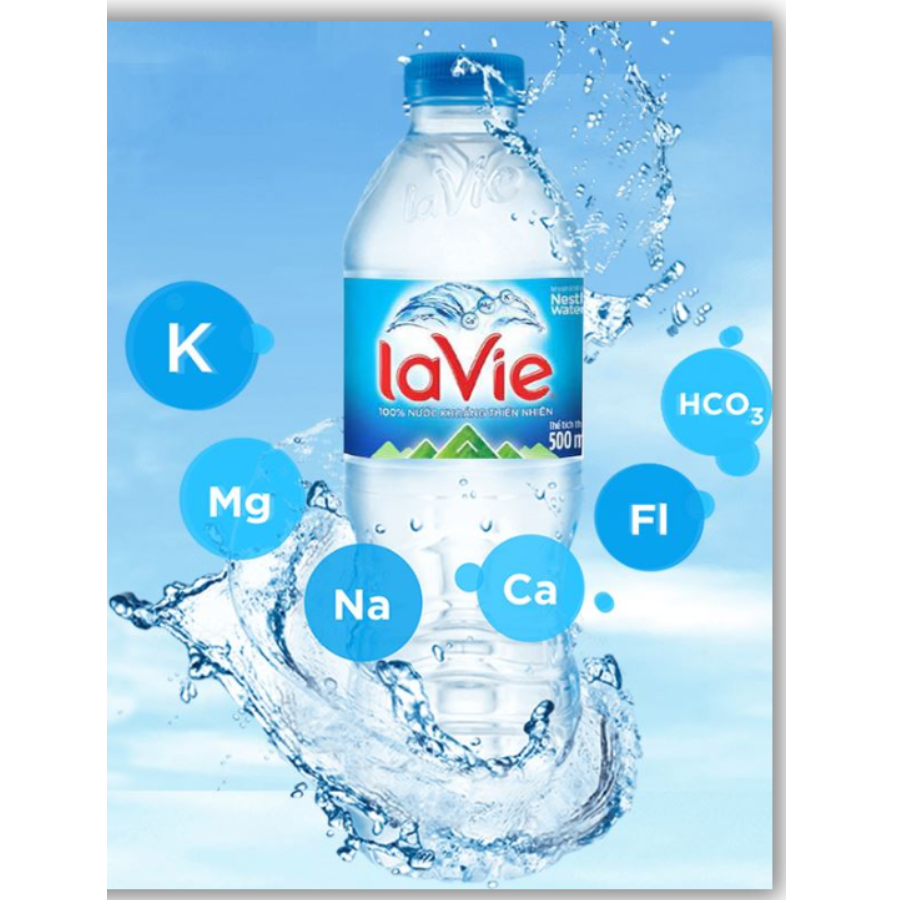
\includegraphics[width=4cm]{Images/anhhoahoc10/nuockhoang.png}}
\end{kd}
\subsection{Nội dung bài học}
\subsubsection{Nguyên tố hóa học}
\begin{paracol}{2}
	\Noibat{Khái niệm nguyên tố hóa học}
	\vspace{0.5cm}
	\begin{tomtat}
		\indam{Nguyên tố hoá học} là tập hợp các nguyên tử có \indam{cùng số đơn vị điện tích hạt nhân} nhưng khác nahu về số neutron. Trong nguyên tử, số đơn vị điện tích hạt nhân bằng số electron ở vỏ nguyên tử. Các electron trong nguyên tử quyết định tính chất hoá học của nguyên tử, nên các nguyên tử của cùng một nguyên tố hoá học có \indam{tính chất hoá học giống nhau}.
	\end{tomtat}
	\switchcolumn
	\begin{Bancobiet}
		Cho đến năm 2020, đã có \indam{118} nguyên tố hoá học được xác định, trong đó \indam{94} nguyên tố có nguồn gốc \indam{tự nhiên}, còn lại là nguyên tớ nhân tạo. Nguyên tố phố biến nhất ở lớp vỏ Trái Đất là oxygen $(\mathrm{O})$, chiếm khoảng $46,6 \%$ khối lượng, tiếp theo là silicon (Si) chiếm khoảng 27,7\% khối lượng.
	\end{Bancobiet}
\end{paracol}
%%%
\Noibat{Số hiệu nguyên tử, số khối, kí hiệu nguyên tử}
\begin{tomtat}
	\begin{enumerate}
		\item Số proton trong hạt nhân được gọi là \indam{số hiệu nguyên tử}.
		\begin{vidu}
			Hạt nhân nguyên tử Oxigen có 8 proton, vậy số hiệu nguyên tử của O là 8 ($Z_{O}=8$)
		\end{vidu}
		\item Tổng số proton ($Z$) và neutron ($N$) trong một hat nhân gọi là \indam{số khối}, kí hiệu là A.
		\[\hopcttoan{\mathsf{A=Z+N}}\]
		\item Kí hiệu nguyên tử $_Z^AX$ cho biết kí hiệu  hóa học của nguyên tố ($X$), số hiệu nguyên tử ($Z$) và số khối ($A$).
		\begin{center}
			\begin{tikzpicture}[declare function={d=1.5;},line cap=round,line join=round]
				\tikzstyle{stylenode} = [color=\maunhan,font=\bfseries\fontsize{25pt}{6pt}\fontfamily{qag}\selectfont,inner sep=3pt,outer sep = 3pt]
				\tikzstyle{stylenodeH} = [anchor=east,color=\maunhan!30!black,font=\bfseries\fontsize{14pt}{0pt}\fontfamily{qag}\selectfont,xshift=2pt,inner sep=3pt,outer sep = 3pt]
				\tikzstyle{stylenodeB} = [font=\small,text width =3cm,inner sep=3pt,outer sep = 3pt]
				%%%
				\path (0,0) node[stylenode] (KHHH) {Al};
				\path (KHHH.north west) node [stylenodeH] (sk) {27};
				\path (KHHH.south west) node [stylenodeH] (shnt) {13};
				\path ($(KHHH)+(d,0)$) node [stylenodeB,anchor=west] (khhh) {Kí hiệu hóa học của nguyên tố};
				\path ($(sk)+({-0.8*d},0)$) node [stylenodeB,anchor=east,align=right] (SK) {Số khối};
				\path ($(shnt)+({-0.8*d},0)$) node [stylenodeB,anchor=east,align=right] (SHNT) {Số hiệu nguyên tử};
				%%%
				\path [fill=\maunhan,rounded corners =4pt,fill opacity=.2] (sk.north west)-|(KHHH.east)|-(shnt.south west)--cycle;
				%%%
				\foreach \x/\y in {KHHH/khhh,SHNT/shnt,SK/sk}
				{\path [draw=\maunhan,thick,shorten <=-0.1cm,shorten >=-0.15cm] (\x)--(\y);}
			\end{tikzpicture}
			\captionof{figure}{Kí hiệu nguyên tử Aluminium}\label{fig:KHHHAl}
		\end{center}
	\end{enumerate}
\end{tomtat}
\subsubsection{Đồng vị, nguyên tử khối trung bình}
\Noibat{Đồng vị}\\
Các nguyên tử của cùng một nguyên tố hóa học có số neutron khác nhau  là đồng vị của nhau
\begin{vidu}[\maunhan]
	Ba loại nguyên tử Oxigen $(\mathrm{O})$ đều có cùng 8 proton trong hạt nhân nên thuộc cùng một nguyên tố hoá học, nguyên tố oxigen $(\mathrm{O})$.
	\begin{center}
		\begin{tikzpicture}[line join=round,line cap=round]
			\tikzset{%
				pics/.cd,
				hinhcau/.style args={#1}{%
					code={\path[pic actions] circle (#1 pt);}
				},
				quydao/.style args={#1}{%
					code={\path[even odd rule,pic actions] circle (#1 cm) circle 	(#1 cm-2pt);}
				}
			}
			%%%===Đồng vị 16========%%%
			\path (0,0) node (m) {\tikz{
					\foreach \p/\m in {
						(0,0)/\maunhan,(45:5pt)/\maunhan,
						(-45:5pt)/\mauphu,(90:5pt)/\mauphu,
						(0:5pt)/\mauphu,(180:5pt)/\mauphu,
						(-135:6pt)/\maunhan,(135:6pt)/\maunhan,
						(-90:7pt)/\maunhan,(90:8pt)/\mauphu,
						(0:8pt)/\maunhan,(180:8pt)/\mauphu,
						(-90:5pt)/\mauphu,(45:8pt)/\maunhan,
						(-30:10pt)/\mauphu,(135:10pt)/\maunhan
					}{
						\path \p pic[ball color=\m] {hinhcau={3}};
					}
					\path (0,0) pic[fill=\maunhan!30]{quydao={1.4}};
					\path (0,0) pic[fill=\maunhan!30]{quydao={1.8}};
					%%%Electron%%%
					%%lop1
					\foreach \g in {0,180}{
						\path (\g:{1.4cm-1pt}) pic[ball color=gray!60!white] {hinhcau={2}};
					}
					%%lop2
					\foreach \g in {45,105,165,215,275,335}{
						\path (\g:{1.8cm-1pt}) pic[ball color=gray!60!white] {hinhcau={2}};
					}
			}};
			%%%===Đồng vị 17========%%%
			\node[right=2cm of m] (h) {\tikz{
					\foreach \p/\m in {
						(0,0)/\mauphu,(45:5pt)/\maunhan,
						(-45:5pt)/\mauphu,(90:5pt)/\maunhan,
						(0:5pt)/\mauphu,(180:5pt)/\maunhan,
						(-135:6pt)/\maunhan,(135:6pt)/\mauphu,
						(-90:7pt)/\maunhan,(90:8pt)/\mauphu,
						(0:8pt)/\mauphu,(180:8pt)/\maunhan,
						(-90:5pt)/\maunhan,(45:8pt)/\mauphu,
						(-30:10pt)/\mauphu,(135:10pt)/\maunhan,
						(-135:11pt)/\mauphu
					}{
						\path \p pic[ball color=\m] {hinhcau={3}};
					}
					\path (0,0) pic[fill=\maunhan!30]{quydao={1.4}};
					\path (0,0) pic[fill=\maunhan!30]{quydao={1.8}};
					%%%Electron%%%
					%%lop1
					\foreach \g in {0,180}{
						\path (\g:{1.4cm-1pt}) pic[ball color=gray!60!white] {hinhcau={2}};
					}
					%%lop2
					\foreach \g in {45,105,165,215,275,335}{
						\path (\g:{1.8cm-1pt}) pic[ball color=gray!60!white] {hinhcau={2}};
					}
					
			}};
			%%%===Đồng vị 18========%%%
			\node [right=2cm of h] (b) {\tikz{
					\foreach \p/\m in {
						(0,0)/\mauphu,(45:5pt)/\maunhan,
						(-45:5pt)/\mauphu,(90:5pt)/\maunhan,
						(0:5pt)/\mauphu,(180:5pt)/\maunhan,
						(-135:6pt)/\maunhan,(135:6pt)/\mauphu,
						(-90:7pt)/\maunhan,(90:8pt)/\mauphu,
						(0:8pt)/\mauphu,(180:8pt)/\maunhan,
						(-90:5pt)/\maunhan,(45:8pt)/\mauphu,
						(-30:10pt)/\mauphu,(135:10pt)/\maunhan,
						(-135:11pt)/\mauphu,(90:11pt)/\mauphu
					}{
						\path \p pic[ball color=\m] {hinhcau={3}};
					}
					\path (0,0) pic[fill=\maunhan!30]{quydao={1.4}};
					\path (0,0) pic[fill=\maunhan!30]{quydao={1.8}};
					%%%Electron%%%
					%%lop1
					\foreach \g in {0,180}{
						\path (\g:{1.4cm-1pt}) pic[ball color=gray!60!white] {hinhcau={2}};
					}
					%%lop2
					\foreach \g in {45,105,165,215,275,335}{
						\path (\g:{1.8cm-1pt}) pic[ball color=gray!60!white] {hinhcau={2}};
					}
			}};
			%%%=====Ghi chú ============
			\path(h.south) node [anchor=north,yshift=-1cm] {\tikz{
					\path (0,0) pic[ball color=gray!60!white,local bounding box=e] 	{hinhcau={4}};
					\node [right= 3pt of e] (electron) {Electron};
					\path ($(electron.east)+(1cm,0)$) pic[ball color=\maunhan,local 	bounding box=p] {hinhcau={6}};
					\node [right= 3pt of p] (proton) {Proton};
					\path ($(proton.east)+(1cm,0)$) pic[ball color=\mauphu,local 	bounding box=n] {hinhcau={6}};
					\node [right= 3pt of n] (notron) {Neutron};
			}};
			%%%===Tên đồng vị===========%%%
			\path (m.south) node[anchor=north,font=\color{\maunhan}\bfseries\small\sffamily]{Đồng vị $_{\phantom{1}8}^{16}O$};
			\path (h.south) node[anchor=north,font=\color{\maunhan}\bfseries\small\sffamily]{Đồng vị $_{\phantom{1}8}^{17}O$};
			\path (b.south) node[anchor=north,font=\color{\maunhan}\bfseries\small\sffamily]{Đồng vị $_{\phantom{1}8}^{18}O$};
		\end{tikzpicture}
		\captionof{figure}{Ba đồng vị phổ biến của Oxigen}
		\label{fig:dongvioxi}
	\end{center}
\end{vidu}
\Noibat{Nguyên tử khối trung bình}
\Noibat[][][\faArrowCircleOLeft]{Nguyên tử khối}

Nguyên tử khối là \indam{khối lượng tương đối} của một nguyên tử, cho biết nguyên tử đó nặng gấp bao nhiêu lần 1 \indam{amu}\footnote{Viết tắt của cụm từ \lq\lq atom mass unit \rq\rq}.

\Noibat[][][\faArrowCircleOLeft]{Nguyên tử khối trung bình}

\indam{Công thức tính nguyên tử khối trung bình:}
\hopcttoan{\overset{\resizebox{0.27cm}{!}{\_}}{\mathsf{A}}=\frac{\mathsf{X} \cdot \mathsf{x}+\mathsf{Y} \cdot \mathsf{y}+\mathsf{Z} \cdot \mathsf{z}+\ldots}{\mathsf{x}+\mathsf{y}+\mathsf{Z}}}\\
Trong đó :
\begin{itemize}
	\item X, Y, Z, $\ldots$ lần lượt là số khối của các đồng vị
	\item x, y, z ,$\ldots$ là phần trăm số nguyên tử các đồng vị tương ứng.
\end{itemize}
\begin{tongket}{Em đã học}
	\begin{itemize}
		\item  Nguyên tố hoá học là tập hợp các nguyên tử có cùng số đơn vị điện tích hạt nhân.
		\item  Đồng vị là những nguyên tử có cùng số đơn vị điện tích hạt nhân (cùng số proton) nhưng có số neutron khác nhau.
		\item  Kí hiệu của nguyên tử: $\mathrm{Z} X$.
		\item  Nguyên tử khối cho biết khối lượng nguyên tử đó nặng gấp bao nhiêu lần đơn vị khối lượng nguyên tử.
		\item  Nguyên tử khối của một nguyên tố là nguyên tử khối trung bình của hỗn hợp các đồng vị của nguyên tố đó.
	\end{itemize}
\end{tongket}

\subsection{Các dạng bài tập}
%%%=========Dạng 1=============%%%
\begin{dang}{Câu hỏi lý thuyết}
	\begin{pp}
		Cần lưu ý một số kiến thức sau:
		\begin{enumerate}
			\item Số khối bằng tổng số hạt proton và nowtron và không có đơn vị và có trị số gần bằng khối lượng nguyên tử (nếu tính theo amu)
			\item nguyên tử khối không có đơn vị, còn khối lượng nguyên tử có đoen vị là amu
			\item Mỗi một nguyên tố có số proton đặc trưng (hoàn toàn khác nhau). Các nguyên tử thuộc cùng một nguyên tố có tính chất hóa học giống nhau.
		\end{enumerate}
	\end{pp}
\end{dang}

%%%Ví dụ mẫu Dạng 1%%%
\Noibat[\maunhan][][\faBookmark]{Ví dụ mẫu}
\hienthiloigiaivd
%%%==============Vidu1==============%%%
\begin{vd}
	Một nguyên tố hóa học được đặc trưng bởi
	\choice
	{\True số proton}
	{số nơtron}
	{số electron}
	{số proton và nơtron}
	\loigiai{Mỗi một nguyên tố được đặc trưng bởi số proton}
\end{vd}
%%%==============HetVidu1==============%%%

%%%==============Vidu2==============%%%
\begin{vd}
	Các nguyên tử thuộc cùng một nguyên tố hóa học đều có
	\choice
	{cùng số nơtron}
	{tính chất hóa học khác nhau}
	{\True tính chất hóa học giống nhau}
	{cùng trọng lượng nguyên tử}
	\loigiai{Các nguyên tử cùng thuộc một nguyên tố có tính chất hóa học giống nhau.}
\end{vd}
%%%==============HetVidu2==============%%%
%%%==============Bài tập tự luyện dạng 1==============%%%
\Noibat[][][\faBank]{Bài tập tự luyện dạng \thedang}
%%%=========Câu hỏi trắc nghiệm 1 phương án=========%%%
\phan{Câu hỏi trắc nghiệm 1 phương án}
\Opensolutionfile{ansex}[Ans/LGEX-Hoa10_C01_CTNT_BTTL01]
\Opensolutionfile{ans}[Ans/Ans-Hoa10_C01_CTNT_BTTL01]
%\hienthiloigiaiex
%\tatloigiaiex
\luuloigiaiex
%%%=============EX_1=============%%%
\begin{ex}
	Nguyên tố hóa học là những nguyên tử có cùng
	\choice
	{số khối}
	{số neutron}
	{\True số proton}
	{số electron}
	\loigiai{Nguyên tố hóa học là tập hợp những nguyên tử  có cùng số proton trong hạt nhân}
\end{ex}
%%%=============EX_2=============%%%
\begin{ex}
	Kí hiệu nguyên tử biểu thị đầy đủ dặc trưng cho một nguyên tử của một nguyên tố hóa học vì nó cho biết
	\choice
	{số khối A}
	{nguyên tử khối của nguyên tử}
	{số hiệu nguyên tử Z}
	{\True số khối A và số hiệu nguyên tử Z}
	\loigiai{Kí hiệu nguyên tử có dạng ${}^{A}_{Z}X$ trong đó X là kí hiệu nguyen tố, A là số khối , Z là số proton }
\end{ex}
%%%=============EX_3=============%%%
\begin{ex}
	Số nơtron trong nguyên tử ${}^{39}_{19}K$ là
	\choice
	{\True$20$}
	{$39$}
	{$19$}
	{$58$}
	\loigiai{ Ta có số neutron được tính theo công thức  $N=A-Z =39-19=20$}
\end{ex}
%%%=============EX_4=============%%%
\begin{ex}
	Trong dãy ký hiệu các nguyên tử sau, dãy nào chỉ cùng một nguyên tố hóa học?
	\choice
	{\True ${}^{12}_{\phantom{0}6}X$, ${}^{13}_{\phantom{0}6}Y$}
	{${}^{18}_{10}Z$, ${}^{14}_{\phantom{0}7}T$}
	{${}^{56}_{26}G$, ${}^{31}_{15}H$}
	{${}^{40}_{20}G$, ${}^{27}_{13}H$}
	\loigiai{Các kí hiệu nguyên tử của cùng một nguyên tố hóa học có cùng số Z (chỉ số góc dưới bên trái kí hiệu nguyên tố)}
\end{ex}
%%%==============Cau_EX5==============%%%
\begin{ex}
	Đốt cháy một chất trong oxi thu được nước và khí cacbonic. Chất đó được cấu tạo bởi những nguyên tố nào?
	\choice
	{Cacbon}
	{Hiđro}
	{Cacbon và hiđro}
	{\True Cacbon, hiđro và có thể có oxi}
	\loigiai{
		
	}
\end{ex}
%%%==============HetCau_EX5==============%%%

%%%==============Cau_EX6==============%%%
\begin{ex}
	Từ một nguyên tố hoá học có thể tạo nên bao nhiêu đợn chất?
	\choice
	{Chỉ 1 đơn chất}
	{Chỉ 2 đơn chất}
	{\True Một, hai hay nhiều đơn chất}
	{Không xác định được}
	\loigiai{}
\end{ex}
%%%==============HetCau_EX6==============%%%

%%%==============Cau_EX7==============%%%
\begin{ex}
	Hợp chất là những chất được tạo nên từ bao nhiêu nguyên tố hoá học?
	\choice
	{Chỉ có 1 nguyên tố}
	{Chỉ từ 2 nguyên tố}
	{Chỉ từ 3 nguyên tố}
	{\True Từ 2 nguyên tố trở lên}
	\loigiai{}
\end{ex}
%%%==============HetCau_EX7==============%%%

%%%==============Cau_EX8==============%%%
\begin{ex}
	Khí ozon gồm 3 nguyên tử oxi. Công thức hóa học của ozon là:
	\choice
	{$30$}
	{$3O_2$}
	{\True $O_3$}
	{$2O_3$}
	\loigiai{}
\end{ex}
%%%==============HetCau_EX8==============%%%
\Closesolutionfile{ansex}
\Closesolutionfile{ans}


%%%=========Dạng 2=============%%%
\begin{dang}{Bài tập về đồng vị và nguyên tử khối trung bình}\end{dang}
%%%bài toán 1%%%
\Noibat[][][\faCoffee]{Bài toán 1: Tính nguyên tử khối trung bình}
\begin{pp}
	Nắm vững công thức : $\overset{\resizebox{0.27cm}{!}{\_}}{A} = \dfrac{X\cdot x+ Y\cdot y + Z\cdot z + \ldots}{x+ y + z +\ldots}$
	
	Trong đó:
	\begin{itemize}
		\item X, Y, Z,\ldots lần lượt là số khối các đồng vị.
		\item x, y, z,\ldots \% số nguyên tử các đồng vị.
	\end{itemize}
\end{pp}
%%%Ví dụ mẫu bài toán 1%%%
\Noibat[\maunhan][][\faBookmark]{Ví dụ mẫu}
\hienthiloigiaivd
%%%=======Bắt đầu ví dụ mau 1========%%%
\begin{vd}
	Oxygen có ba đồng vị với tỉ lệ phần trăm số nguyên tử tương ứng là ${}^{16}\mathrm{O}(99{,}757\%)$, ${}^{17}\mathrm{O}(0{,}038\%)$, ${}^{18}\mathrm{O}(0{,}205\%)$. Nguyên tử khối trung bình của oxygen là bao nhiêu amu?
	\loigiai{
		Nguyên tử khối trung bình của Oxigen là
		\begin{eqnarray*}
			\overset{-\phantom{-}}{A_{O}} & = & \dfrac{16 \cdot 99{,}757 + 17 \cdot 0{,}038 + 18 \cdot 0{,}205 }{100}\\
			& \approx & 16{,}0 \text{~amu}
		\end{eqnarray*}
		Vậy, nguyên tử khối trung bình của oxygen là khoảng $16{,}0$ amu.
	}
\end{vd}
%%%=======Kết thúc ví dụ mau 1========%%%

%%%============bài toán 2=======================%%%
\Noibat[][][\faCoffee]{Bài toán 2: Tính phần trăm số nguyên tử mỗi đồng vị}
\begin{pp}
	Dùng phương pháp đại số (đặt ẩn - giải hệ)
	\Noibat{Các bước giải:}
	\begin{cacbuoc}
		\item Đặt ẩn là phần trăm số nguyên tử các đồng vị
		\item Kết hợp công thức tính nguyên tử khối trung bình
		\[\overset{\resizebox{0.27cm}{!}{\_}}{A} = \dfrac{A_1\cdot x_1+ A_2\cdot x_2 + A_3\cdot x_3 + \ldots}{x_1+ x_2 + x_3 +\ldots}\] với mối liên hệ tổng phần trăm số nguyên tử các đồng vị $x_1 +x_2 + x_3 +\ldots =100$ để lập hệ phương trình
	\end{cacbuoc}
\end{pp}
%%%Ví dụ mẫu bài toán 2%%%
\Noibat[\maunhan][][\faBookmark]{Ví dụ mẫu}
%%%==============Bat dau_VDM2==============%%%
\begin{vd}
	Boron là nguyên tố có nhiều tác dụng đối với cơ thể người như: làm lành vết thương, điều hoà nội tiết sinh dục, chống viêm khớp,\ldots Do ngọn lửa cháy có màu lục đặc biệt nên boron vô định hình được dùng làm pháo hoa. Boron có hai đồng vị là $^{10} \mathrm{~B}$ và $^{11} \mathrm{~B}$, nguyên tử khối trung bình là 10,81. Tính phần trăm số nguyên tử mỗi đồng vị của boron.
	\loigiai{
		Gọi x, y lần lượt là phần trăm số nguyên tử của $\phantom{.}^{10}B$ và $\phantom{.}^{11}B$.
		\\
		Theo đề bài ta có nguyên tử khối trung bình của Bo là $10{,}81$ nên ta có phương trình:
		\[\begin{aligned}
			&\dfrac{10x +11y}{x+y}=10{,}81&\\
			\Leftrightarrow \,& 0{,}81x -0{,}19y= 0 &\quad\left(1\right)\\
		\end{aligned}\]
		Mặt khác, ta có $x+y =100$ \quad $\left(2\right)$
		\\
		Từ $\left(1\right)$ và $\left(2\right)$ ta có hệ phương trình 
		$\heva{&0{,}81x -0{,}19y =0\\&x+y=100}$.
		Giải hệ ta được $\heva{&x=19\\&y=81}$.
		\\
		Vậy phần trăm số nguyên tử của $\phantom{.}^{10}B$ là $19\%$ và của $\phantom{.}^{11}B$ là $81\%$
	}
\end{vd}
%%%==============HetBai_VDM2==============%%%

%%%===================bài toán 3============================%%%
\Noibat[][][\faCoffee]{Bài toán 3: Đếm số loại phân tử}
\begin{pp}
	-- Liệt kê các đồng vị của các nguyên tố trong phân tử.
	\\
	-- Tổ hợp các đồng vị hình thành phân tử đã cho
\end{pp}
\Noibat[\maunhan][][\faBookmark]{Ví dụ mẫu}
%%%=============VDM 3=============%%%
\begin{vd}
	Carbon có hai đồng vị bền là $_6^{12} \mathrm{C}$ và $_6^{13} \mathrm{C}$. Oxygen có ba đồng vị bền là $_8^{16} O,_8^{17} O$ và $_8^{18} O$. Số hợp chất $CO_2$ tạo bởi các đồng vị trên là
	\choice
	{$9$}
	{\True$12$}
	{$18$}
	{$27$}
	\loigiai{Xét hợp chất $CO_2$ có dạng \canhdong{\chemfig[atom sep=3em]{O_a-[:30]C-[:-30]O_b}}
		\\
		Để tạo ra một phân tử $CO_2$ cần 1 nguyên tử $C$ và 2 nguyên tử $O$
		\begin{itemize}
			\item Chọn 1 nguyên tử C trong 2 đồng vị C có 2 cách chọn
			\item Chọn 2 nguyên tử O
			\begin{itemize}
				\item TH1 : $O_a \equiv O_b$ có 3 cách chọn
				\\
				$\Rightarrow$ Số loại phân tử $CO_2$ được tạo ra là $2\times3 =6$ (phân tử)
				\item TH2 :$O_a \neq O_b$ có 3 cách chọn
				\\
				$\Rightarrow$ Số loại phân tử $CO_2$ được tạo ra là $2\times3 =6$ (phân tử)
			\end{itemize}
			
		\end{itemize}
		Vậy có tất cả  $6+6=12$ (phân tử)
	}
\end{vd}
%%%===================bài toán 3============================%%%
\Noibat[][][\faCoffee]{Bài toán 4: Phần trăm khối lượng đồng vị trong hợp chất}
\begin{pp}
	\begin{cacbuoc}
		\item Lấy số mol hợp chất bằng 1 mol
		\item Từ đó tính được số mol mỗi đồng vị
		\item Tính phần trăm khối lượng mỗi đồng vị
	\end{cacbuoc}
\end{pp}
\Noibat[\maunhan][][\faBookmark]{Ví dụ mẫu}
%%%=============VDM4=============%%%
\begin{vd}
	Trong tự nhiên, nguyên tố Clo có 2 đồng vị bền là ${}^{35}_{17}Cl$ và ${}^{37}_{17}Cl$, trong đó đồng vị ${}^{35}_{17}Cl$ chiếm $75{,}00\%$ về số nguyên tử. Phần trăm khối lượng của ${}^{37}_{17}Cl$ trong $CaCl_2$ là
	\choice
	{$15{,}99\%$}
	{$15{,}77\%$}
	{\True $16{,}67\%$}
	{$47{,}97\%$}
	\loigiai{
		Ta có $\% ^{35}\mathrm{Cl} + \% ^{37}\mathrm{Cl} =100 \%  \Rightarrow \% ^{37}\mathrm{Cl}=100\% - 75\% =25\%$
		\\
		Nguyên tử khối trung bình của Cl là: $\overset{\_}{A}_{Cl}= \dfrac{35\cdot75+37\cdot25}{100}=35{,}5$
		\\
		Gọi số mol của $CaCl_2$ là $1$ mol $\Rightarrow n _{Cl} =1\cdot2=2$ mol
		\\
		Do đó: $n_{^{37}Cl} =2\cdot0{,}25=0{,}5$ mol
		\begin{eqnarray*}
			\Rightarrow \% m_{^{37}Cl} &=&\dfrac{m_{^{37}Cl}}{m_{CaCl_2}}\cdot100\% \\
			&=&\dfrac{37 \cdot 0{,}5}{(40+35{,}5\cdot2)}\cdot100\% = 16{,}67
		\end{eqnarray*}
		Vậy phần trăm khối lượng của ${}^{37}_{17}Cl$ trong $CaCl_2$ là $16{,}67 \%$
	}
\end{vd}

%%%==============Bài tập tự luyện dạng 2==============%%%
\Noibat[][][\faBank]{Bài tập tự luyện dạng \thedang}
%%%=========Câu hỏi trắc nghiệm 1 phương án=========%%%
\phan{Câu hỏi trắc nghiệm 1 phương án}
\Opensolutionfile{ansex}[Ans/LGEX-Hoa10_C01_CTNT_BTTL02]
\Opensolutionfile{ans}[Ans/Ans-Hoa10_C01_CTNT_BTTL02]
%\hienthiloigiaiex
%\tatloigiaiex
\luuloigiaiex
%%%=============EX_5=============%%%
\begin{ex}
	Clo có hai đồng vị là ${}^{35}_{17}Cl$ và ${}^{37}_{17}Cl$. Cho biết khối lượng nguyên tử trung bình của clo là $35{,}5$. Phần trăm số nguyên tử của đồng vị ${}^{37}_{17}Cl$ trong hỗn hợp là
	\choice
	{$75\%$}
	{$40\%$}
	{$60\%$}
	{\True$25\%$}
	\loigiai{
		Gọi phần trăm số nguyên tử của đồng vị ${}^{37}_{17}Cl$ trong hỗn hợp là $x \%$\\
		Ta có
		\begin{eqnarray*}
			& \overset{\_}{A}_{Cl} & = 35{,}5\\
			\Leftrightarrow &\dfrac{37 \cdot x + 35 \cdot (100-x)}{100} & = 35{,}5\\
			\Leftrightarrow & x & = 25
		\end{eqnarray*}
		Vậy phần trăm số nguyên tử của đồng vị ${}^{37}_{17}Cl$ là $25\%$
	}
\end{ex}
%%%=============EX_6=============%%%
\begin{ex}
	Hỗn hợp 2 đồng vị bền của một nguyên tố có nguyên tử khối trung bình là $40{,}08$. Hai đồng vị này có số nơtron hơn kém nhau hai hạt. Đồng vị có số khối lớn hơn chiếm $4\%$ về số nguyên tử. Số khối lớn là
	\choice
	{$40$}
	{\True$42$}
	{$41$}
	{$43$}
	\loigiai{
		Giả sử nguyên tố  có 2 đồng vị bền là $_{\phantom{Z}Z}^{A_1}X$ và $_{\phantom{Z}Z}^{A_2}X$ với ($A_2>A_1$).
		\\
		Ta có {\renewcommand{\arraystretch}{0.85}
			$\left.
			\begin{aligned}
				A_1=Z+N_1\\
				A_2=Z+N_2
			\end{aligned}
			\right\}$}
		$\Rightarrow A_2-A_1=N_2-N_1 =2$ hay $-A_1+A_2=2$ (1)
		\\
		Mặt khác theo đề bài ta có \[
		\begin{aligned}
			&&\overset{\_}{A}_{X}& = 40{,}08&\\
			&\Leftrightarrow &\dfrac{ A_1\times 96 + A_2 \times 4}{100}& = 40{,}08&\\
			&\Leftrightarrow &96A_1+4A_2& = 4008 & \quad (2)
		\end{aligned}
		\]
		Từ (1) và (2) ta có hệ phương trình $\heva{&-A_1+A_2&=&\phantom{x}2\\&96A_1+4A_2&=&\phantom{x}4008}$.
		Giải hệ ta được $\heva{&A_1=40\\&A_2=42}$
		\\
		Vậy Số khối lớn hơn là $42$.
	}
\end{ex}
%%%=============EX_7=============%%%
\begin{ex}
	Một nguyên tố X có 3 đồng vị là $X_1$, $X_2$ và $X_3$. Đồng vị $X_1$ chiếm $92{,}23\%$, $X_2$ chiếm $4{,}67\%$ và $X_3$ chiếm $3{,}10\%$ số nguyên tử. Tổng số khối của 3 đồng vị bằng $87$. Số nơtron trong đồng vị $X_2$ nhiều hơn số nơtron trong đồng vị $X_1$ là một hạt. Nguyên tử khối trung bình của X là $28{,}0855$ và trong $X_1$ có số nơtron bằng số proton. Số nơtron của $X_2$ là
	\choice
	{$14$}
	{$15$}
	{$13$}
	{$16$}
	\loigiai{
		Gọi ba đồng vị của X lần lượt là $_{\phantom{z}Z}^{A_1}X_1$, $_{\phantom{z}Z}^{A_2}X_2$ và $_{\phantom{z}Z}^{A_3}X_3$
		\\
		Theo giả thiết ta có $A_1+A_2+A_3=87$ (1)
		\\
		Vì $N_2-N_1=1$ $\Rightarrow$ $A_2-A_1=1$ (2)
		\\
		Lại có $\overset{\_}{A}_X=28{,}0855 \Leftrightarrow 0{,}9223A_1+0{,}0467A_2+0{,}031A_3=28{,}0855$ (3).
		\\
		Từ (1), (2) và (3) ta có hệ phương trình $\heva{&A_1+A_2+A_3=87\\&-A_1+A_2=1\\&0{,}9223A_1+0{,}0467A_2+0{,}031A_3=28{,}0855}$.
		\\
		Giải hệ ta được $\heva{&A_1=28\\&A_2=29\\&A_3=30}$
		$\Rightarrow N_1 =Z =\dfrac{A_1}{2}=\dfrac{28}{2}=14\Rightarrow N_2 =15$
		\\
		Vậy số neutron của $X_2 = 15 $ (hạt)
	}
\end{ex}
%%%=============EX_8=============%%%
\begin{ex}
	Trong tự nhiên, Clo có hai đồng vị bền là ${}^{37}_{17}Cl$ chiếm $24{,}23\%$ tổng số nguyên tử, vậy còn lại là ${}^{35}_{17}Cl$. Thành phần phần trăm theo khối lượng của ${}^{35}_{17}Cl$ trong $HClO_4$ là
	\choice
	{$8{,}43\%$}
	{\True $8{,}79\%$}
	{$8{,}92\%$}
	{$8{,}5\%$}
	\loigiai{
		Ta có $\% ^{37}\mathrm{Cl} = 24{,}23\% \Rightarrow \% ^{35}\mathrm{Cl} = 100\% - 24{,}23\% = 75{,}77\%$
		\\
		Nguyên tử khối trung bình của Cl là:
		\begin{eqnarray*}
			\overset{\_}{A}_{Cl} &=& \dfrac{35 \cdot 75{,}77 + 37 \cdot 24{,}23}{100} \\
			&=& \dfrac{2651{,}95 + 896{,}51}{100} \\
			&=& 35{,}4846
		\end{eqnarray*}
		Gọi số mol của $HClO_4$ là $1$ mol $\Rightarrow n_{Cl} = 1$ mol
		\\
		Do đó: $n_{^{35}Cl} = 1 \cdot 0{,}7577 = 0{,}7577$ mol
		\\
		Khối lượng phân tử của $HClO_4$:
		\begin{eqnarray*}
			M_{HClO_4} &=& 1 + 35{,}4846 + 4 \cdot 16 \\
			&=& 100{,}4846 \text{ g/mol}
		\end{eqnarray*}
		\\
		Tính phần trăm khối lượng của ${}^{35}_{17}Cl$ trong $HClO_4$:
		\begin{eqnarray*}
			\% m_{^{35}Cl} &=& \dfrac{m_{^{35}Cl}}{m_{HClO_4}} \cdot 100\% \\
			&=& \dfrac{35 \cdot 0{,}7577}{100{,}4846} \cdot 100\% \\
			&=& 8{,}79\%
		\end{eqnarray*}
		\\
		Vậy thành phần phần trăm theo khối lượng của ${}^{35}_{17}Cl$ trong $HClO_4$ là $8{,}79\%$
	}
\end{ex}
%%%=============EX_9=============%%%
\begin{ex}
	Nguyên tố $Cu$ có hai đồng vị, nguyên tử khối trung bình là $63{,}62$.Một trong hai đồng vị là $^{63}Cu$ (chiếm $69{,}17\%$).Nguyên tử khối của đồng vị thứ hai là
	\choice
	{$66$}
	{$64$}
	{$67$}
	{\True$65$}
	\loigiai{Gọi nguyên tử khối của đồng vị thứ hai là $x$.
		Ta có phương trình:
		\[
		\begin{aligned}
			&&63 \cdot 0{,}6917 + x\cdot(1-0{,}6917)= 63{,}62 &\\
			\Leftrightarrow	&&x = 65 &
		\end{aligned}
		\]
		Vậy nguyên tử khối của đồng vị thứ hai là $65$ (amu).
	}
\end{ex}
%%%=============EX_10=============%%%
\begin{ex}
	Nguyên tố $Cl$ có hai đồng vị, nguyên tử khối trung bình là $35{,}48$.Một trong hai đồng vị là $^{35}Cl$ (chiếm $75{,}78\%$).Nguyên tử khối của đồng vị thứ hai là
	\choice
	{$38$}
	{$36$}
	{$39$}
	{\True$37$}
	\loigiai{Gọi nguyên tử khối của đồng vị thứ hai là $x$.
		Ta có phương trình:
		\[
		\begin{aligned}
			&&35 \cdot 0{,}7578 + x\cdot(1-0{,}7578)= 35{,}48 &\\
			\Leftrightarrow	&&x = 37 &
		\end{aligned}
		\]
		Vậy nguyên tử khối của đồng vị thứ hai là $37$ (amu).
	}
\end{ex}
%%%=============EX_11=============%%%
\begin{ex}
	Nguyên tố $K$ có ba đồng vị, nguyên tử khối trung bình là $39{,}13$.Hai trong ba đồng vị là $^{39}K$ (chiếm $93{,}2581\%$) và $^{40}K$ (chiếm $0{,}0117\%$).Nguyên tử khối của đồng vị thứ ba là
	\choice
	{$40$}
	{$43$}
	{\True$41$}
	{$42$}
	\loigiai{Gọi nguyên tử khối của đồng vị thứ ba là $x$.
		Ta có phương trình:
		\[
		\begin{aligned}
			&&39 \cdot 0{,}932581 +40 \cdot 0{,}000117 + x\cdot(1-0{,}932581-0{,}000117)= 39{,}13 &\\
			\Leftrightarrow	&&x = 41 &
		\end{aligned}
		\]
		Vậy nguyên tử khối của đồng vị thứ ba là $41$ (amu).
	}
\end{ex}
%%%=============EX_12=============%%%
\begin{ex}
	Nitrogen có hai đồng vị bền là $_7^{14} \mathrm{N}$ và $_7^{15} \mathrm{N}$. Hydrogen có ba đồng vị bền là $_1^{1} \mathrm{H}$ , $_1^{2} \mathrm{H}$ và $_1^{3} \mathrm{H}$. Số hợp chất $NH_3$ tạo bởi các đồng vị trên là
	\choice
	{$12$}
	{\True $14$}
	{$24$}
	{$32$}
	\loigiai{
		Xét hợp chất $NH_3$ có dạng \chemfig[atom sep=4em,bond offset=4pt]{H_a-[:35]N(<[:-60]H_c)<:[:-20]H_b}
		\\
		Để tạo ra một phân tử $NH_3$ cần 1 nguyên tử $N$ và 3 nguyên tử $H$
		\begin{itemize}
			\item Chọn 1 nguyên tử N trong 2 đồng vị N có 2 cách chọn
			\item Chọn 3 nguyên tử H
			\begin{itemize}
				\item TH1 : $H_a \equiv H_b \equiv H_c $ có 3 cách chọn
				\\
				$\Rightarrow$ Số loại phân tử $NH_3$ được tạo ra là $2\times3 =6$ (phân tử)
				\item TH2 :$H_a \equiv H_b \neq H_c $ có 3 cách chọn
				\\
				$\Rightarrow$ Số loại phân tử $NH_3$ được tạo ra là $2\times3 =6$ (phân tử)
				\item TH3 :$H_a \neq H_b \neq H_c $ có 1 cách chọn
				\\
				$\Rightarrow$ Số loại phân tử $NH_3$ được tạo ra là $2\times1 =2$ (phân tử)
			\end{itemize}
			
		\end{itemize}
		Vậy có tất cả  $6+6+2=14$ (phân tử)
	}
\end{ex}
\Closesolutionfile{ans}
\Closesolutionfile{ansex}
%\bangdapan{Ans-Hoa10_C01_CTNT_BTTL02}

%%%============Câu hỏi đúng sai================%%%
\phan{Câu hỏi trắc nghiệm đúng sai}
%%%%====================%%%
\Opensolutionfile{ansex}[Ans/LGTF-Hoa10_C01_CTNT_BTTL02]
\Opensolutionfile{ansbook}[Ansbook/AnsTF-Hoa10_C01_CTNT_BTTL02]
\Opensolutionfile{ans}[Ans/Tempt-Hoa10_C01_CTNT_BTTL02]
\luulgEXTF
%%%=============EX_15=============%%%
\begin{ex}
	Nguyên tố Mg có KHNT là ${}^{24}_{12}Mg$.Hãy cho biết tính đúng, sai của các phát biểu sau:
	\choiceTF[t]
	{\True Magnesium có 12 proton và 12 electron}
	{\True Magnesium có số khối là 24}
	{Magnesium có nguyên tử khối là 24 amu}
	{Ion $Mg^{2+}$ có 10 electron trong hạt nhân}
	\loigiai{
		\begin{itemchoice}
			\itemch Đúng. Trong một nguyên tử trung hòa tổng số proton = tổng số electron
			\itemch Đúng. Theo kí hiệu nguyên tố ${}^A_ZX$ trong đó $A$ là số khối, $Z$ là số hiệu nguyên tử
			\itemch Sai. Nguyên tử khối  không có đơn vị
			\itemch Sai. Electron nằm ở vỏ nguyên tử, proton và neutron  nằm trong hạt nhân. Nguyên tử trung hòa khi mất đi electron ở lớp vỏ ngoài cùng sẽ tạo thành ion dương (cation).
		\end{itemchoice}
	}
\end{ex}
%%%=============EX_16=============%%%
\begin{ex}
	Cho biết nguyên tử khối trung bình của Clo là 35,5 u. Biết rằng Clo tồn tại dưới dạng hai đồng vị ${}^{35}_{17}Cl$ và ${}^{37}_{17}Cl$. Hãy cho biết tính đúng, sai của các phát biểu sau:
	\choiceTF[t]
	{\True Nguyên tố Clo có 17 proton trong hạt nhân}
	{\True Tỉ lệ phần trăm của đồng vị ${}^{35}_{17}Cl$ là 75\%}
	{Số neutron của đồng vị ${}^{37}_{17}Cl$ là 37}
	{Nguyên tử khối trung bình của Clo là trung bình cộng của hai đồng vị}
	\loigiai{
		\begin{itemchoice}
			\itemch Đúng. Số proton trong hạt nhân bằng số hiệu nguyên tử (17).
			\itemch Đúng. Gọi x là tỉ lệ phần trăm của ${}^{35}_{17}Cl$, ta có: 35x + 37(100-x) = 35,5 * 100. Giải ra được x = 75\%.
			\itemch Sai. Số neutron của đồng vị ${}^{37}_{17}Cl$ là 37 - 17 = 20.
			\itemch Sai. Nguyên tử khối trung bình được tính bằng trung bình có trọng số của các đồng vị, không phải trung bình cộng đơn giản.
		\end{itemchoice}
	}
\end{ex}
\Closesolutionfile{ans}
\Closesolutionfile{ansbook}
\Closesolutionfile{ansex}
%\bangdapanTF{AnsTF-Hoa10_C01_CTNT_BTTL02}
%%%================Phần tự luận================%%%
\phan{Bài tập tự luận}
\Opensolutionfile{ansbth}[Ans/LGBT-Hoa10_C01_CTNT_BTTL02]
\Opensolutionfile{ansbt}[Ans/AnsBT-Hoa10_C01_CTNT_BTTL02]
\luuloigiaibt
%\hienthiloigiaibt
%%%=============BT_1=============%%%
\begin{bt}
	Chromium (Cr), có khối lượng các đồng vị và độ phổ biến được cho ở bảng sau (Bảng \ref{tab:dvCr}). Hãy tính nguyên tử khối trung bình của Chromium
	\begin{center}
		\begin{tabular}{*{3}{C{0.26\linewidth}}}
			\hline\rowcolor{\maunhan!5}
			\begin{tabular}{l}
				\textsf{\textbf{Số khối}}
			\end{tabular}
			&
			\begin{tabular}{l}
				\textsf{\textbf{Khối lượng đồng vị}}
			\end{tabular}
			&
			\begin{tabular}{l}
				\textsf{\textbf{Độ phổ biến}}
			\end{tabular}
			\\
			\hline
			50 & 49{,}9461 & 0{,}0435 \\
			52 & 51{,}9405 & 0{,}8379 \\
			53 & 52{,}9407 & 0{,}0950 \\
			54 & 53{,}9389 & 0{,}0236 \\
			\hline
		\end{tabular}
		\captionof{table}{Các đồng vị phổ biến của 	Chromium } \label{tab:dvCr}
	\end{center}
	\loigiai{Nguyên tử khối của Cr là:
		\[
		\begin{aligned}
			\overset{\_}{A}_{Cr}&=49{,}9461\cdot0{,}0435+49{,}9461\cdot0{,}0435+52{,}9407\cdot0{,}0950+53{,}9389\cdot 0{,}0236 \\
			&= 51{,}9959 \approx 52
		\end{aligned}
		\]
		Vậy khối lượng nguyên tử trung bình của Cr là 52 (amu)
	}
\end{bt}
%%%=============BT_2=============%%%
\begin{bt}
	Hoàn thành những thông tin còn thiếu trong bảng sau:\\
	\begin{tabular}{|c|c|c|c|}
		\hline
		\rowcolor{\maunhan!8}
		Nguyên tử & Kí hiệu nguyên tử & Số hiệu nguyên tử & Số khối \\
		\hline
		Zinc & $_{30}^{65} \mathrm{Zn}$ & $?$ & $?$ \\
		\hline
		Carbon & $?$ & $6$ & $14$ \\
		\hline
		Lead & $_{82}^? \mathrm{Pb}$ & $?$ & $207$ \\
		\hline
		Oxygen & $_{8}^{16} \mathrm{O}$ & $?$ & $?$ \\
		\hline
		Copper & $?$ & $29$ & $64$ \\
		\hline
		Iron & $_{26}^? \mathrm{Fe}$ & $?$ & $56$ \\
		\hline
	\end{tabular}
	\loigiai{
		\begin{tabular}{|c|c|c|c|}
			\hline
			\rowcolor{\maunhan!8}
			Nguyên tử & Kí hiệu nguyên tử & Số hiệu nguyên tử & Số khối \\
			\hline
			Zinc & $_{30}^{65} \mathrm{Zn}$ & $30$ & $65$ \\
			\hline
			Carbon & $_{6}^{14} \mathrm{C}$ & $6$ & $14$ \\
			\hline
			Lead & $_{82}^{207} \mathrm{Pb}$ & $82$ & $207$ \\
			\hline
			Oxygen & $_{8}^{16} \mathrm{O}$ & $8$ & $16$ \\
			\hline
			Copper & $_{29}^{64} \mathrm{Cu}$ & $29$ & $64$ \\
			\hline
			Iron & $_{26}^{56} \mathrm{Fe}$ & $26$ & $56$ \\
			\hline
		\end{tabular}
	}
\end{bt}
%%%=============BT_3=============%%%
\begin{bt}
	Hoàn thành những thông tin còn thiếu trong bảng sau:
	\\
	\begin{tabular}{|c|c|c|c|}
		\hline
		Nguyên tử & Ki hiệu nguyên tử & Số hiệu nguyên tử & Số khối \\
		\hline
		Europium & $_{63}^{152} \mathrm{Eu}$ & $?$ & $?$ \\
		\hline
		Silver & $?$ & 47 & 108 \\
		\hline
		Tellurium & $_{52}^? \mathrm{Te}$ & $?$ & 128 \\
		\hline
	\end{tabular}
	\loigiai{
		\begin{tabular}{|c|c|c|c|}
			\hline
			Nguyên tử & Ki hiệu nguyên tử & Số hiệu nguyên tử & Số khối \\
			\hline
			Europium & $_{63}^{152} \mathrm{Eu}$ & $63$ & $152$ \\
			\hline
			Silver & $_{47}^{108} \mathrm{Ag}$ & $47$ & $108$ \\
			\hline
			Tellurium & $_{52}^{128} \mathrm{Te}$ & $52$ & $128$ \\
			\hline
		\end{tabular}
	}
\end{bt}
%%%=============BT_4=============%%%
\begin{bt}
	Hoàn thành những thông tin còn thiếu trong bảng sau:
	\\
	\begin{tabular}{|c|c|c|c|}
		\hline
		\rowcolor{\maunhan!8}
		Nguyên tử & Kí hiệu nguyên tử & Số hiệu nguyên tử & Số khối \\
		\hline
		Iodine & $_{\phantom{x}53}^{127} \mathrm{I}$ & $?$ & $?$ \\
		\hline
		Gold & $?$ & $79$ & $197$ \\
		\hline
		Platinum & $_{78}^? \mathrm{Pt}$ & $?$ & $195$ \\
		\hline
		Sulfur & $_{16}^{32} \mathrm{S}$ & $?$ & $?$ \\
		\hline
		Tin & $?$ & $50$ & $119$ \\
		\hline
		Barium & $_{56}^? \mathrm{Ba}$ & $?$ & $137$ \\
		\hline
	\end{tabular}
	\loigiai{
		\begin{tabular}{|c|c|c|c|}
			\hline
			\rowcolor{\maunhan!8}
			Nguyên tử & Kí hiệu nguyên tử & Số hiệu nguyên tử & Số khối \\
			\hline
			Iodine & $_{\phantom{x}53}^{127} \mathrm{I}$ & $53$ & $127$ \\
			\hline
			Gold & $_{\phantom{x}79}^{197}\mathrm{Au}$ & $79$ & $197$ \\
			\hline
			Platinum & $_{78}^{195} \mathrm{Pt}$ & $78$ & $195$ \\
			\hline
			Sulfur & $_{16}^{32} \mathrm{S}$ & $16$ & $32$ \\
			\hline
			Tin & $_{50}^{119} \mathrm{Sn}$ & $50$ & $119$ \\
			\hline
			Barium & $_{56}^{137} \mathrm{Ba}$ & $56$ & $137$ \\
			\hline
		\end{tabular}
	}
\end{bt}

%%%=============BT_7=============%%%
\begin{bt}
	Chlorine có hai đồng vị với tỉ lệ phần trăm số nguyên tử tương ứng là ${}^{35}\mathrm{Cl}(75{,}77\%)$ và ${}^{37}\mathrm{Cl}(24{,}23\%)$. Nguyên tử khối trung bình của chlorine là bao nhiêu amu?
	\loigiai{
		Nguyên tử khối trung bình của chlorine là
		\begin{eqnarray*}
			\overset{-\phantom{-}}{A_{Cl}} & = & \dfrac{35 \cdot 75{,}77 + 37 \cdot 24{,}23}{100} \\
			& \approx & 35{,}5 \text{~amu}
		\end{eqnarray*}
		Vậy, nguyên tử khối trung bình của chlorine là khoảng $35{,}5$ amu.
	}
\end{bt}
% Bài tập 2

%%%=============BT_8=============%%%
\begin{bt}
	Copper có hai đồng vị với tỉ lệ phần trăm số nguyên tử tương ứng là ${}^{63}\mathrm{Cu}(69{,}17\%)$ và ${}^{65}\mathrm{Cu}(30{,}83\%)$. Nguyên tử khối trung bình của copper là bao nhiêu amu?
	\loigiai{
		Nguyên tử khối trung bình của copper là
		\begin{eqnarray*}
			\overset{-\phantom{-}}{A_{Cu}} & = & \dfrac{63 \cdot 69{,}17 + 65 \cdot 30{,}83}{100} \\
			& \approx & 63{,}5 \text{~amu}
		\end{eqnarray*}
		Vậy, nguyên tử khối trung bình của copper là khoảng $63{,}5 $amu.
	}
\end{bt}
% Bài tập 3

%%%=============BT_9=============%%%
\begin{bt}
	Silicon có ba đồng vị với tỉ lệ phần trăm số nguyên tử tương ứng là ${}^{28}\mathrm{Si}(92{,}23\%)$, ${}^{29}\mathrm{Si}(4{,}67\%)$, ${}^{30}\mathrm{Si}(3{,}10\%)$. Nguyên tử khối trung bình của silicon là bao nhiêu amu?
	\loigiai{
		Nguyên tử khối trung bình của silicon là
		\begin{eqnarray*}
			\overset{-\phantom{-}}{A_{Si}} & = & \dfrac{28 \cdot 92{,}23 + 29 \cdot 4{,}67 + 30 \cdot 3{,}10}{100} \\
			& \approx & 28{,}0 \text{~amu}
		\end{eqnarray*}
		Vậy, nguyên tử khối trung bình của silicon là khoảng $28{,}0$ amu.
	}
\end{bt}
% Bài tập 4

%%%=============BT_10=============%%%
\begin{bt}
	Bromine có hai đồng vị với tỉ lệ phần trăm số nguyên tử tương ứng là ${}^{79}\mathrm{Br}(50{,}69\%)$ và ${}^{81}\mathrm{Br}(49{,}31\%)$. Nguyên tử khối trung bình của bromine là bao nhiêu amu?
	\loigiai{
		Nguyên tử khối trung bình của bromine là
		\begin{eqnarray*}
			\overset{-\phantom{-}}{A_{Br}} & = & \dfrac{79 \cdot 50{,}69 + 81 \cdot 49{,}31}{100} \\
			& \approx & 80{,}0 \text{~amu}
		\end{eqnarray*}
		Vậy, nguyên tử khối trung bình của bromine là khoảng $80{,}0$ amu.
	}
\end{bt}

%%%=============BT_11=============%%%
\begin{bt}
	\Rightpicture[0.47]{%
		Trong tự nhiên, Neon (kí hiệu Ne) khi phân tích phổ khối lượng như biểu đồ sau (xem hình \ref{fig:phoMS_neon})
		\begin{enumerate}
			\item Neon có bao nhiêu đồng vị bền?
			\item Tính nguyên tử khối trung bình của neon?
		\end{enumerate}
	}{%
		\begin{center}
			\resizebox{!}{4cm}{
				\begin{tikzpicture}[line join=round,line cap=round,declare function={d=0.2cm;}]
					\pgfmathsetmacro{\hsa}{1.5}
					\pgfmathsetmacro{\hsb}{18}
					%%% Vẽ 2 truc tọa độ
					\draw [thick,-latex,\maunhan] (0,0)coordinate (xw)--(9,0)coordinate (xe) node 	[below]{(m/z)};
					\draw [thick,-latex,\maunhan] (0,0)coordinate (ys)--(0,5.5)coordinate (yn) 	node[right]{(\%)};
					%%% Các giá trị truc y
					\foreach \y[evaluate =\y as \yt using int(\y*20)] in {1,...,5}{
						\draw[\maunhan!80!black] (0.1,\y)--+(180:0.2) node 		[left,font=\small\bfseries]{\yt};
					}
					%%% Các giá trị truc x
					\foreach \x [evaluate =\x as \xt using int(\x+\hsb)] in {1,...,5}{
						\draw[\maunhan!80!black] (\hsa*\x,0.1)--+(-90:.2) node 		[below,font=\small\bfseries]{\xt};
					}
					%%% Vẽ cột
					\foreach \x/\y[evaluate =\y as \yt using \y*20] in {
						2/4.545,3/0.015,4/0.44
					}{
						\path[fill=\maunhan!80] ([xshift=-d]\hsa*\x,0) rectangle +({2*d},\y) node 	[above,xshift=-d,font=\bfseries\color{\maunhan!60!black}] {\pgfmathprintnumber[fixed, precision=2,use comma]{\yt}};
					}
					%%% Hiển thị thông tin trục y
					\path ([xshift=-1.2cm]ys)--([xshift=-1.2cm]yn) node 	[pos=0.5,midway,sloped,font =\scriptsize \color{\maunhan!50!black}\bfseries\sffamily]{Phần trăm số nguyên tử đồng vị};
					%%% Hiển thị thông tin trục x
					\path ([yshift=-0.9cm]xw)--([yshift=-0.9cm]xe) node 	[pos=0.5,midway,sloped,font 	=\scriptsize\color{\maunhan!50!black}\bfseries\sffamily]{Tỉ số nguyên tử khối/điện tích};
				\end{tikzpicture}
			}
			\captionof{figure}{Phổ khối lượng của Neon}\label{fig:phoMS_neon}
		\end{center}
	}
	\loigiai{
		\begin{enumerate}
			\item Neon có ba đồng vị bền là $_{10}^{20}Ne$$(90{,}9\%)$, $_{10}^{21}Ne$$(0{,}3\%)$,  $_{10}^{22}Ne$$(8{,}8\%)$.
			\item Nguyên tử khối trung bình của Neon là:
			\[
			\begin{aligned}
				\overset{\gachngang\phantom{aai}}{A_{Ne}}=\dfrac{20\cdot90{,}9+21\cdot0{,}3+22\cdot8{,}8}{100}=20{,}179 (amu)
			\end{aligned}
			\]
		\end{enumerate}
	}
\end{bt}

%%%=============BT_12=============%%%
\begin{bt}
	\Rightpicture[0.47]{%
		Trong tự nhiên, Zirconium (kí hiệu Zr) khi phân tích phổ khối lượng như biểu đồ sau (xem hình \ref{fig:phoMS_Zr})
		\begin{enumerate}
			\item Zirconium có bao nhiêu đồng vị bền?
			\item Tính nguyên tử khối trung bình của Zirconium?
		\end{enumerate}
	}{%
		\begin{center}
			\resizebox{!}{4cm}{
				\begin{tikzpicture}[line join=round,line cap=round,declare function={d=0.2cm;}]
					\pgfmathsetmacro{\hsa}{1.3}
					\pgfmathsetmacro{\hsb}{89}
					%%% Vẽ 2 truc tọa độ
					\draw [thick,-latex,\maunhan] (0,0)coordinate (xw)--(10.5,0)coordinate (xe) node 	[below]{(m/z)};
					\draw [thick,-latex,\maunhan] (0,0)coordinate (ys)--(0,5.5)coordinate (yn) 	node[right]{(\%)};
					%%% Các giá trị truc y
					\foreach \y[evaluate =\y as \yt using int(\y*20)] in {1,...,5}{
						\draw[\maunhan!80!black] (0.1,\y)--+(180:0.2) node 		[left,font=\small\bfseries]{\yt};
					}
					%%% Các giá trị truc x
					\foreach \x [evaluate =\x as \xt using int(\x+\hsb)] in {1,...,7}{
						\draw[\maunhan!80!black] (\hsa*\x,0.1)--+(-90:.2) node 		[below,font=\small\bfseries]{\xt};
					}
					%%% Vẽ cột
					\foreach \x/\y[evaluate =\y as \yt using \y*20] in {
						1/2.5725,2/0.561,3/0.8575,5/0.869,7/0.14
					}{
						\path[fill=\maunhan!80] ([xshift=-d]\hsa*\x,0) rectangle +({2*d},\y) node 	[above,xshift=-d,font=\bfseries\color{\maunhan!60!black}] {\pgfmathprintnumber[fixed, precision=2,use comma]{\yt}};
					}
					%%% Hiển thị thông tin trục y
					\path ([xshift=-1.2cm]ys)--([xshift=-1.2cm]yn) node 	[pos=0.5,midway,sloped,font =\scriptsize \color{\maunhan!50!black}\bfseries\sffamily]{Phần trăm số nguyên tử đồng vị};
					%%% Hiển thị thông tin trục x
					\path ([yshift=-0.9cm]xw)--([yshift=-0.9cm]xe) node 	[pos=0.5,midway,sloped,font 	=\scriptsize\color{\maunhan!50!black}\bfseries\sffamily]{Tỉ số nguyên tử khối/điện tích};
				\end{tikzpicture}
			}
			\captionof{figure}{Phổ khối lượng của Zirconium}\label{fig:phoMS_Zr}
		\end{center}
	}
	\loigiai{
		\begin{enumerate}
			\item Zirconium có năm đồng vị bền là $_{40}^{90}Zr$$(51.45\%)$, $_{40}^{91}Zr$$(11.22\%)$, $_{40}^{92}Zr$$(17.15\%)$, $_{40}^{94}Zr$$(17.38\%)$, và $_{40}^{96}Zr$$(2.80\%)$.
			\item Nguyên tử khối trung bình của Zirconium là:
			\[
			\begin{aligned}
				\overset{\gachngang\phantom{aai}}{A_{Zr}}=\dfrac{90 \cdot 51.45 + 91 \cdot 11.22 + 92 \cdot 17.15 + 94 \cdot 17.38 + 96 \cdot 2.80}{100} \approx 91.224 \, \text{amu}
			\end{aligned}
			\]
		\end{enumerate}
	}
\end{bt}
%%%=============BT_13=============%%%
\begin{bt}
	Đồng vị phóng xạ cobalt $(\mathrm{Co}-60)$ phát ra tia $\gamma$ có khả năng đâm xuyên mạnh, dùng điều trị các khối u ở sâu trong cơ thể. Cobalt có ba đồng vị: $_{27}^{59} \mathrm{Co}$ (chiếm $98\%$), $_{27}^{58} \mathrm{Co}$ và $_{27}^{60} \mathrm{Co}$; nguyên tử khối trung bình là 58,982. Xác định hàm lượng $\%$ của đồng vị phóng xạ Co-60.
	\loigiai{
		Gọi x, y lần lượt là phần trăm số nguyên tử của $\phantom{.}^{58}Co$ và $\phantom{.}^{60}Co$.
		\\
		Theo đề bài ta có nguyên tử khối trung bình của Co là $58{,}982$ nên ta có phương trình:
		\[
		\begin{aligned}
			&\dfrac{58x +60y+59\cdot98}{100}=58{,}982&\\
			\Leftrightarrow \,& 58x +60y= 116{,}2 &\quad\left(1\right)\\
		\end{aligned}
		\]
		Mặt khác, ta có $x+y+98 =100$ hay $x+y = 2$ $\left(2\right)$
		\\
		Từ $\left(1\right)$ và $\left(2\right)$ ta có hệ phương trình
		$\heva{&58x +60y= 116{,}2\\&x+y = 2}$.
		Giải hệ ta được $\heva{&x=1{,}9\\&y=0{,}1}$.
		\\
		Vậy phần trăm số nguyên tử của $\phantom{.}^{60}Co$ là $0{,}1\%$
	}
\end{bt}
%%%=============BT_14=============%%%
\begin{bt}
	Oxide của kim loại $M$ $(M_2O_3)$ được ứng dụng rộng rãi trong công nghiệp, đặc biệt trong sản xuất thép không gỉ và làm chất xúc tác. Trong phòng thí nghiệm, $M_2O_3$ thường có màu xanh lục đến xám đen và ít tan trong nước. Tổng số hạt cơ bản trong phân tử $X$ có công thức $M_2O_3$ là 218, trong đó số hạt mang điện nhiều hơn số hạt không mang điện là 70.Biết nguyên tử oxi có 8 proton và 8 neutron. Xác định công thức phân tử của $M_2O_3$.
	\loigiai{
		Gọi $Z_M$, $N_M$ lần lượt là số proton và neutron của M.
		\\
		Trong $M_2O_3$ có tổng số hạt trong phân tử là $218$ và số hạt không mang điện nhiều hơn số hạt không mang điện là $70$ hạt nên ta có:
		$\heva{& 2\cdot(2Z_M + 3Z_O) + (2N_M+3N_O)=218\\
			&2\cdot(2Z_M + 3Z_O) - (2N_M+3N_O)=70
		}$ (*)
		\\
		Mặt khác ta có $Z_O=N_O=8$ (**)
		\\
		Từ (*) và (**) suy ra $\heva{&Z_M=24 \\&N_M=25 
		}$ $\Rightarrow M$  là  $Cr$.
		\\
		Vậy công thức phân tử của oxide là $Cr_2O_3$.
	} 
\end{bt}
%%%==============Bai_BT15==============%%%
\begin{bt}
	Oxide của kim loại $M\left(M_2O\right)$ được ứng dụng rất nhiều trong ngành hoá chất như sản xuất xi măng, sản xuất phân bón,\ldots Trong sản xuất phân bón, chúng ta thường thấy $M_2O$ có màu trắng, tan nhiều trong nước và là thành phần không thể thiếu cho mọi loại cây trồng. Tồng số hạt cơ bản trong phân tử X có công thức $M_2O$ là 140, trong phân tử X có tồng số hạt mang điện nhiều hơn số hạt không mang điện là 44. Xác định công thức phân tử của $M_2O$.
	\loigiai{
		Gọi $Z_M$, $N_M$ lần lượt là số proton và neutron của M.
		\\
		Trong $M_2O$ có tổng số hạt trong phân tử là $140$ và số hạt không mang điện nhiều hơn số hạt không mang điện là $44$ hạt nên ta có:
		$\heva{& 2\cdot(2Z_M + Z_O) + (2N_M+N_O)=140\\
			&2\cdot(2Z_M + Z_O) - (2N_M+N_O)=44
		}$
		\\
		$\Rightarrow \heva{& 2Z_M + Z_O=\dfrac{140+44}{4}=46 \phantom{x}(*)\\
			&2N_M+N_O=\dfrac{140-44}{2}=48
		}$ 
		Thay $Z_O=8$ vào (*) ta được $Z_M =19 $  $\Rightarrow $ M là K
		\\
		Vậy công thức phân tử của oxide là $K_2O$.
	}
\end{bt}
%%%==============HetBai_BT15==============%%%

%%%==============Bai_BT16==============%%%
\begin{bt}
	Hợp chất $XY_2$ phổ biến trong sử dụng để làm cơ chế đánh lửa bằng bánh xe trong các dạng súng cổ. Mỗi phân từ $XY_2$ có tồng các hạt proton, neutron, electron bằng 178; trong đó, số hạt mang điện nhiều hơn số hạt không mang điện là 54, số hạt mang điện của X ít hơn số hạt mang điện của Y là 12. Hãy xác định kí hiệu hoá học của $X, Y$.
	\loigiai{
		Gọi $Z_X$, $N_X$ lần lượt là số proton và neutron của X và $Z_Y$, $N_Y$ lần lượt là số proton và neutron của Y.
		\\
		Trong $XY_2$ có tổng số hạt trong phân tử là $178$ và số hạt không mang điện nhiều hơn số hạt không mang điện là $54$ hạt nên ta có:
		$\heva{& 2\cdot(Z_X + 2Z_Y) + (N_X+2N_Y)=178\\
			&2\cdot(Z_X + 2Z_Y) - (N_X+2N_Y)=54
		}$
		$\Rightarrow \heva{& Z_X + 2Z_Y=\dfrac{178+54}{4}=58 \phantom{x}(*)\\
			&N_X+2N_Y=\dfrac{178-54}{2}=62
		}$ 
		\\
		Mặt theo đề bài ta có : $2Z_X +12=4Z_Y$ (**)
		\\
		Từ (*) và (**) ta có hệ phương trình $\heva{
			&2Z_X - 4Z_Y=-12\\
			&Z_X + 2Z_Y=58
		}$ $\Leftrightarrow $  $\heva{
			&Z_X =26\\
			&Z_Y =16}$.
		Vậy $X$ là Fe và Y là S.
	}
\end{bt}
%%%==============HetBai_BT16==============%%%
\Closesolutionfile{ansbt}
\Closesolutionfile{ansbth}
%\bangdapanSA{AnsBT-Hoa10_C01_CTNT_BTTL02}
%%%==========Nội dung file thứ 3===============%%%
\section{Cấu trúc lớp vỏ electron}
\begin{Muctieu}
	\begin{itemize}
		\item  Trình bày và so sánh được nô hình của Rutherford - Bohr với mô hình hiện đại mô tả sự chuyển động của electron trong nguyên tử
		\item  Nêu được klái niệm về orbital nguyên tử $(\mathrm{AO})$, mô tả được hìnl dạng của $\mathrm{AO}(\mathrm{s}$, số lượng electron trong 1 AO .
		\item  Trìh bày được khái niệm lớp, phân lớp electron và mối quan hệ về số lượng phân trong một lớp. Liên hệ được về số lượng AO trong một phân lớp, trong một lớp.
		\item  Viết được cấu lình electron nguyên tử theo lớp, phân lớp electron và theo ô orbital biết số liệu nguyên tử $Z$ của 20 nguyên tố đầu tiên trong bảng tuần hoàn.
		\item  Dựa vào đặc điểm cấu hình electron lớp ngoài cùng của nguyên tử, dự đoán được chất hoá học cơ bản (kim loại hay pli kim) của nguyên tố tương ưng.
	\end{itemize}
\end{Muctieu}
\subsection{Nội dung bài học}
\subsubsection{Sự chuyển động của electron trong nguyên tử}
\Noibat[][][\faArrowCircleORight]{Các mô hình nguyên tử}
\begin{figure}[!htp]
	\begin{center}
		\subcaptionbox{Mô hình nguyên tử Borh-Rutherford\label{atomic_borh}}[0.4\textwidth]
		{\begin{tikzpicture}[declare function={R=2;r=0.3*R;}]
				\tikzset{%
					pics/.cd,
					hinhcau/.style args={#1}{%
						code={\path[pic actions] circle (#1 pt);}
					},
				}
				%%%Khai bao gốc tạo độ
				\path (0,0) coordinate (O);
				%%%Hạt nhân
				\foreach \g/\c/\d in {0/\maunhan/0,40/\mauphu/4,80/\mauphu/8,120/\maunhan/8,160/\mauphu/7,220/\maunhan/7,280/\mauphu/7,340/\maunhan/8,40/\maunhan/8}{
					\path ($(O)+(\g:\d pt)$) pic[ball color =\c] {hinhcau={4.5}};
				}
				%%% Quỹ đạo e
				\foreach \goc/\p in {30/30,90/50,150/90}{
					\path[left color=\mycolor,right color =\maunhan,line width=2pt,even odd rule,rotate around={\goc:(O)}] 
					(O) ellipse ({R} and {r}) (O) ellipse ({0.98*R} and {0.96*r})
					;
					\path ($(O)+(180:{0.99*R})$) arc (180:\p:{0.99*R} and {0.98*r}) coordinate (G);
					\path (G) pic[ball color =\mauphu,rotate around={\goc:(O)}] {hinhcau={3}};
				}
		\end{tikzpicture}}
		\subcaptionbox{Mô hình nguyên tử hiện đại\label{atomic_modern}}[0.4\textwidth]
		{\begin{tikzpicture}[declare function={R=2;r=0.3*R;}]
				\tikzset{%
					pics/.cd,
					hinhcau/.style args={#1}{%
						code={\path[pic actions] circle (#1 pt);}
					},
				}
				%%%Khai bao gốc tạo độ
				\path (0,0) coordinate (O);
				%%%vong tron trong
				\path[fill opacity=0.52,fill=\mauphu!90!black,path fading=fade in one](O) circle (2.2cm);
				%%%Dam may e
				\foreach \i in {1,...,2000}
				{
					\pgfmathsetmacro{\angle}{random()*360}
					\pgfmathsetmacro{\u}{random()}
					\pgfmathsetmacro{\radius}{2.18 * pow(\u, 2)}  
					\pgfmathsetmacro{\x}{\radius*cos(\angle)}
					\pgfmathsetmacro{\y}{\radius*sin(\angle)}
					\path (\x,\y) pic[fill=\mauphu,path fading=fade in three] {hinhcau={0.65}};
				}
				%%%Hạt nhân
				\path[fill=\maudam!70!white,path fading=fade in four](O) circle (0.48cm);
				\foreach \g/\c/\d in {0/\maunhan/0,40/\mauphu/4,80/\mauphu/8,120/\maunhan/8,160/\mauphu/7,220/\maunhan/7,280/\mauphu/7,340/\maunhan/8,40/\maunhan/8}{
					\path ($(O)+(\g:\d pt)$) pic[ball color =\c] {hinhcau={4.5}};
				}
				%%%vong tron ngoài
				\path[fill opacity=0.50,fill=\mauphu,path fading=fade in one](O) circle (2.2cm);
		\end{tikzpicture}}
		\caption{Hai Mô hình nguyên tử }\label{fig:atomic_model}
	\end{center}
\end{figure}
\begin{hoivadap}
	\begin{cauhoi}
		Quan sát hình \ref{atomic_borh} và hình \ref{atomic_modern} so sánh điểm giống và khác nhau giữa mô hình Rutherford - Bohr với mô hình hiện đại mô tả sự chuyển động của electron trong nguyên tử.
	\end{cauhoi}
	\loigiai{
		\begin{longtable}{|C{0.25\textwidth}|p{0.33\textwidth}|p{0.33\textwidth}|}
			\caption{So sánh hai mô hình nguyên tử}\label{tab:ssmhnt}\\
			\hline\rowcolor{\maunhan!20}
			\makecell[c]{\qagfont{Tiêu chí}} & \makecell[c]{\qagfont{Mô hình Rutherford-Bohr}} & \makecell[c]{\qagfont{Mô hình hiện đại}} \\
			\hline
			\endfirsthead
			\multicolumn{3}{c}%
			{{\bfseries \tablename\ \thetable{} -- tiếp theo}} \\
			\hline\rowcolor{\maunhan!20}
			\makecell[c]{\qagfont{Tiêu chí}} & \makecell[c]{\qagfont{Mô hình Rutherford-Bohr}} & \makecell[c]{\qagfont{Mô hình hiện đại}} \\
			\hline
			\endhead
			\hline \multicolumn{3}{|r|}{{Tiếp theo ở trang sau}} \\ \hline
			\endfoot
			\hline
			\endlastfoot
			\multirow[c]{2.5}{*}{\makecell[c]{\textcolor{\maunhan}{\textbf{Cấu trúc nguyên tử}}}} & Hạt nhân ở trung tâm, electron chuyển động quanh hạt nhân theo các quỹ đạo tròn & Hạt nhân ở trung tâm, electron chuyển động trong các obitan (đám mây electron) \\
			\hline
			\multirow[c]{2.0}{*}{\makecell[c]{\textcolor{\maunhan}{\textbf{Quỹ đạo electron}}}} & Các quỹ đạo tròn cố định với bán kính xác định & Obitan - vùng không gian có xác suất tìm thấy electron cao \\
			\hline
			\multirow[c]{2.5}{*}{\makecell[c]{\textcolor{\maunhan}{\textbf{Năng lượng electron}}}} & Electron chỉ tồn tại ở các mức năng lượng xác định (trạng thái dừng) & Electron có thể tồn tại ở nhiều mức năng lượng khác nhau trong một obitan \\
			\hline
			\multirow[c]{2.5}{*}{\makecell[c]{\textcolor{\maunhan}{\textbf{Chuyển động}}\\\textcolor{\maunhan}{\textbf{của electron}}}} & Chuyển động tròn quanh hạt nhân & Chuyển động phức tạp, không thể xác định chính xác vị trí và vận tốc cùng lúc \\
			\hline
			\textcolor{\maunhan}{\textbf{Nguyên lý xác định vị tríelectron}} & Có thể xác định chính xác vị trí và vận tốc của electron & Tuân theo nguyên lý bất định Heisenberg \\
			\hline
			\textcolor{\maunhan}{\textbf{Sự mô tả electron}} & Hạt & Lưỡng tính sóng-hạt \\
			\hline
			\textcolor{\maunhan}{\textbf{Số lượng electron tối đa trên một lớp}} & 2n\textsuperscript{2} (n là số lớp) & Tuân theo nguyên lý Pauli và quy tắc Hund \\
			\hline
			\multirow[c]{2}{*}{\makecell[c]{\textcolor{\maunhan}{\textbf{Hình dạng obitan}}}} & Không đề cập & Có nhiều hình dạng khác nhau (s, p, d, f) \\
			\hline
			\multirow[c]{2}{*}{\makecell[c]{\textcolor{\maunhan}{\textbf{Spin của electron}}}} & Không đề cập & Được xem xét và ảnh hưởng đến cấu hình electron \\
			\hline
			\multirow[c]{2}{*}{\makecell[c]{\textcolor{\maunhan}{\textbf{Giải thích phổ}}\\ \textcolor{\maunhan}{\textbf{nguyên tử}}}} & Giải thích được phổ của nguyên tử hydro & Giải thích được phổ của tất cả các nguyên tử \\
		\end{longtable}
	}
\end{hoivadap}
\Noibat[][][\faArrowCircleORight]{Tìm hiểu về orbital nguyên tử}
\Noibat{Khái niệm}
\vspace{0.5cm}
\begin{tomtat}
	Orbital nguyên tử (ki hiệu là AO) là khu vực không gian xung quanh hạt nhân nguyên tử mà xác suất tìm thấy electron trong khu vực đó là lớn nhất (khoảng $90 \%$ ).
\end{tomtat}
\begin{hopvidu}[\maunhan]
	\begin{itemize}
		\item Các AO thường gặp là s, p, d, f.
		\item Orbital nguyên tử có một số hình dạng khác nhau. Ví dụ: AO hình cầu, còn gọi là $\mathrm{AO} \mathrm{s} ; \mathrm{AO}$ hình số tám nổi, còn gọi là AO p (tùy theo vị tri của AO p trên hệ trục toạ độ Descartes (Đề-các), sẽ gọi là $\mathrm{AO} \mathrm{p}_{\mathrm{x}}, \mathrm{P}_{\mathrm{y}}$ và $\mathrm{p}_z$ )(xem hình \ref{fig:hinhdangAO}).
	\end{itemize}
\end{hopvidu}
\begin{hopvidu}[\mycolor]
	\begin{center}
		\begin{tikzpicture}[declare function={d=1cm;r=.55*d;h=.125*d;R=.36*d;k=0.65*d;}]
			\tikzstyle{linestyle} = [line width=1pt,\maunhan!80]
			\tikzstyle{myshapestyle} = [line width=1pt,opacity=.90,ball color =\mauphu!90]
			\tikzset{
				pics/.cd,
				AOs/.style args={#1/#2}{code={%
						\if\relax\detokenize{#1}\relax
						\def\ballcolor{red}
						\else
						\def\ballcolor{#1}
						\fi,
						\if\relax\detokenize{#2}\relax
						\def\opacity{0.8}
						\else
						\def\opacity{#2}
						\fi
						\draw[linestyle] ([xshift=-1.8*R]0*d,0)--([xshift=1.8*R]0*d,0);
						\fill[myshapestyle,ball color = \ballcolor,opacity=\opacity] (0*d,0) circle (R);
				}},
				AOp/.style args={#1/#2}{code={%
						\draw[linestyle,pic actions] (0,{-1.5*d - h})--(0,{1.5*d + h}) node [pos=#2,above,font=\sffamily\bfseries] {#1};
						\path[myshapestyle,pic actions] (0,0)..controls +(0:{.25*r}) and +(0:r)..(0,d)--
						(0,d)..controls +(180:r) and +(180:{.25*r})..(0,0);
						\path[myshapestyle] (0,-d)..controls +(180:r) and +(180:{.25*r})..(0,0)--
						(0,0)..controls +(0:{.25*r}) and +(0:r)..(0,-d);
				}}
			}
			\path (0*k,0) coordinate (A)
			(4*k,0) coordinate (B)
			(9*k,0) coordinate (C)
			(13*k,0) coordinate (D)
			;
			\path (A) pic [local bounding box=AOsa] {AOs={red}/{}};
			\path (B) pic[local bounding box=AOPx,rotate around={-45:(B)},<-,>=stealth]  {AOp={x}/{0}};
			\path (C) pic [local bounding box=AOPy,rotate around={-90:(C)},-latex] at (C) {AOp={y}/{1}};
			\path (D)  pic [local bounding box=AOPz,-latex] at (D) {AOp={z}/{1}};
			\foreach \p/\n in {
				A/AOs,B/AOpx,C/AOpy,D/AOpz
			}{
				\path ($(\p)+ (0,-2)$) node [inner sep =0pt, outer sep =0pt,font=\bfseries\sffamily] {\n};
			}
		\end{tikzpicture}
	\end{center}
	\captionof{figure}{Hình dạng các AO s và AOp\label{fig:hinhdangAO}}
\end{hopvidu}
\Noibat{Ô orbital}
\vspace{0.5cm}
\begin{tomtat}
	\begin{itemize}
		\item Một AO được biểu diễn bằng một ô vuông, gọi là ô orbital \raisebox{-3pt}{\squarerow[][0.5][\mycolor]{1}}
		\item Trong 1 orbital chỉ chứa tối đa 2 electron có chiều tự quay ngược nhau (nguyên lí loại trừ Pauli (Pau-li)). Nếu orbital có 1 electron thì biểu diễn bằng 1 mũi tên đi lên (\raisebox{-3pt}{\squarerow[1u][0.5][\mycolor]{1}}), nếu orbital có 2 electron thì được biểu diễn bằng 2 mũi tên ngược chiều nhau, mũi tên đi lên viết trước (\raisebox{-3pt}{\squarerow[2ud][0.5][\mycolor]{1}}).
	\end{itemize}
\end{tomtat}
\subsubsection{Lớp và phân lớp electron}
\Noibat[][][]{Lớp electron}\\
\begin{tomtat}
	\begin{enumerate}
		\item Thứ tự các lớp electron được ghi bằng các số nguyên $n=1, 2, 3, ... , 7$.
		\item Các electron thuộc cùng một lớp có mức năng lương gần bằng nhau
	\end{enumerate}
\end{tomtat}
\vspace{0.5cm}
\begin{center}
	\captionof{table}{\textbf{Tên gọi các lớp từ 1 đến 7}\label{lopelectron}}
	\begin{tabular}{C{0.1\linewidth}*{7}{C{0.1\linewidth}}}
		\textbf{n}&1&2&3&4&5&6&7\\
		\textbf{Tên lớp} &K&L&M&N&O&P&Q
	\end{tabular}
\end{center}
\Noibat[][][]{Phân lớp electron}\\
\begin{tomtat}
	\begin{enumerate}
		\item  Mỗi lớp electron phân chia thành các phân lớp được kí hiệu bằng các chữ cái viết thường: s, p, d, f.
		\item  Các electron trên cùng một phân lớp có mức năng lượng bằng nhau.
		\item  Số phân lớp trong mỗi lớp bằng số thứ tự của lớp $(n \leq 4)$ :
	\end{enumerate}
\end{tomtat}
\begin{vidu}
	\begin{itemize}
		\item Lớp thứ nhất (lớp K) có 1 phân lớp , đó là phân lớp 1s
		\item Lớp thứ hai (lớp L) có 2 phân lớp , đó là phân lớp 2s và 2p
		\item Lớp thứ ba (lớp M) có 3 phân lớp , đó là các phân lớp 3s, 3p và 3d
		\item Lớp thứ 4 (lớp N) có 4 phân lớp , đó là các phân lớp 4s, 4p, 4d, 4f
	\end{itemize}
\end{vidu}
\Noibat{Số lượng Orbital trong một lớp, phân lớp}
\Noibat[][][\faAngleRight][][0.25]{Số lượng Orbital trong một phân lớp}
\begin{tomtat}
	Trong một phân lớp, các orbital có cùng mức năng lượng.
	\begin{itemize}
		\item Phân lớp s có 1 AO s
		\item Phân lớp p có 3 AO px, py, pz
		\item Phân lớp d có 5 AO 
		\item Phân lớp f có 7 AO 
	\end{itemize}
\end{tomtat}
\Noibat[][][\faAngleRight][][0.25]{Số lượng Orbital trong một lớp}
\begin{tomtat}
	Số obitan trong lớp electron thứ n là $n^2$ orbital
	\begin{itemize}
		\item Lớp K (n=1) có $1^2 =1$ AO đó là AO 1s.
		\item Lớp L (n=2) có $2^2 =4$ AO đó là 1 AO 2s và 3 AO 2p.
		\item Lớp M (n=3) có $3^2 =9$ AO đó là 1 AO 3s, 3 AO 3p và  5 AO 3d.
		\item Lớp N (n=4) có $4^2 =16$ AO đó là 1 AO 4s, 3 AO 4p, 5AO 4d và 7 AO 4f.
	\end{itemize}
\end{tomtat}
\begin{hoivadap}
	\begin{cauhoi}
		Hãy cho biết số electron  tối đa có trong một phân lớp , một lớp?
	\end{cauhoi}
	\loigiai{
		Số AO có trong các phân lớp s,p,d,f  tương ứng là 1, 3, 5, 7 và mỗi AO chứa tối đa 2 electron do đó
		\begin{itemize}[wide=0.65cm]
			\item Phân lớp s chứa tối đa $2\cdot1 =2$ electron
			\item Phân lớp p có chứ tối đa $2\cdot3 =6$  electron
			\item Phân lớp d chứa tối đa $2\cdot5 =10$  electron
			\item Phân lớp f có tối đa $2\cdot7 =14$  electron
		\end{itemize}
		Lớp n có $n^2$ AO do đó số electron tối đa có trong lớp electron thứ n là $2n^2$
	}
\end{hoivadap}
\subsubsection{Cấu hình electron của nguyên tử}
\Noibat{Năng lượng của electron trong nguyên tử}
\Noibat[][][\faArrowCircleORight]{Trật tự mức năng lượng AO}\\
\begin{tomtat}
	\begin{itemize}
		\item Khi số hiệu nguyên tử $Z$ tăng, các mức năng lượng $AO$ tăng dần theo trình tự sau:
	\end{itemize}
	\centering\boxct[\maunhan][3pt][\color{\maunhan}\qagfont]{1s 2s 2p 3s 3p 4s 3d 4p 5s 4d 5s 4d 5p 6s 4f 5d 6p 4f 5d 6p 7s 5f 6d \ldots}
\end{tomtat}
\Noibat[][][\faArrowCircleORight]{Nguyên lý và quy tắc phân bố electron trong nguyên tử}
\begin{ghinho}
	\indam{Nguyên lý Pau-ly.}Trên một obitan chỉ có thể nhiều nhất là hai electron và hai electron này chuyển động tự quay khác chiều nhau xung quanh trục riêng của mỗi electron.
\end{ghinho}

Như vậy theo nguyên lý Pau-li thì:
\begin{itemize}[wide=0.65cm]
	\item lớp n có tối đa $2n^2$ electron
	\item Số electron tối đa trên các phân lớp s, p, d, f lần lượt là $2$, $6$, $10$, $14$ electron
\end{itemize}

\begin{hopvidu}[\maunhan]
	\begin{itemize}[wide=0.65cm,leftmargin=0.65cm]
		\item Để biểu thị phân lớp 1s có 2 electron  ta dùng kí hiệu $1s^2$.Trong đó:số 1 chỉ lớp n=1. Chữ s chỉ orbital s. Số 2 ở phía trên bên phải số electron có trong AO s.
		\item Phân lớp: $s^2$,$p^6$, $d^{10}$, $f^{14}$ có đủ electron tối đa gọi là \indam{phân lớp bão hòa}.
		\item Phân lớp $s^1$,$p^3$, $d^5$, $f^7$ có nửa số electron tối đa gọi là \indam{phân lớp bán bão hòa}.
		\item Phân lớp chưa đủ số electron tối đa gọi là \indam{phân lớp chưa bão hòa}.Ví dụ $s^1$, $p^3$, $p^5$, $d^9$, $f^{11}$.
	\end{itemize}
\end{hopvidu}

\begin{note}
	Người ta biểu thị chiều tự quay khác nhau quanh trục riêng của hai electron bằng 2 mũi tên nhỏ:Một mũi tên có chiều đi lên  và một mũi tên có chiều đi xuống . 
	\begin{itemize}[wide=0.65cm,leftmargin=0.65cm]
		\item Trong 1 orbital đã có 2 electron, thì 2 electron này gọi là \indam{electron ghép đôi} .Khi biểu diễn mũi tên bên trái phải vẽ hướng lên và mũi tên bên phải vẽ hướng xuống (\squarerow[2ud][0.5][\maunhan][-4pt]{1})
		\item Trong một Orbital chỉ có 1 electron, thì electron này gọi là  \indam{electron độc thân}. Khi biểu diễn mũi tên bắt buộc phải vẽ chiều hướng lên (\squarerow[1u][0.5][\maunhan][-4pt]{1})
	\end{itemize}
\end{note}
\begin{ghinho}
	\indam{Nguyên lý vững bền.} Các electron trong nguyên tử ở trạng thái cơ bản lần lượt chiếm các mức năng lượng từ thấp đến cao.
\end{ghinho}
\begin{vidu}
	Nguyên tử helium ($Z=2$) có 2 electron. Theo nguyên lý pau - li hai electron này cùng chiếm orbital 1s có mức năng lượng thấp nhất. Do đó sự phân bố electron trên orbital của He là \[1s^2 \xrightarrow \squarerow[2ud][0.5][\maunhan][-4pt]{1}\]
	Nguyên tử Boron ($Z=5$) có 5 electron. 2 electron đầu tiên chiếm AO 1s có năng lượng thấp nhất, 2 eletcron tiếp theo chiếm AO 2s và electron còn lại chiếm AO 2p . Do đó sự phân bố electron trên orbital của B là \[1s^22s^22p^1 \xrightarrow \underset{1s^2}{\squarerow[2ud][0.5][\maunhan][-4pt]{1}}\; \underset{2s^2}{\squarerow[2ud][0.5][\maunhan][-2pt]{1}}\hspace{-0.8pt} \underset{2p^1}{\squarerow[1u][0.5][\maunhan][0pt]{3}}\].
\end{vidu}
\begin{ghinho}
	\indam{Quy tắc Hund.} Trong cùng một phân lớp, các electron sẽ phân bố trên các obitan sao cho số electron độc thân là tối đa và các electron này phải có chiều tự quay giống nhau.
\end{ghinho}
\begin{vidu}
	Sự phân bố electron trên các orbital của carbon và nitrogen như sau: \[ C(Z=6):\quad \underset{1s^2}{\squarerow[2ud][0.5][\maunhan][-4pt]{1}}\; \underset{2s^2}{\squarerow[2ud][0.5][\maunhan][-2pt]{1}}\hspace{-0.8pt} \underset{2p^2}{\squarerow[1u,1u][0.5][\maunhan][0pt]{3}} \hspace{2cm}
	N(Z=7):\quad \underset{1s^2}{\squarerow[2ud][0.5][\maunhan][-4pt]{1}}\; \underset{2s^2}{\squarerow[2ud][0.5][\maunhan][-2pt]{1}}\hspace{-0.8pt} \underset{2p^3}{\squarerow[1u,1u][0.5][\maunhan][0pt]{3}}
	\].
\end{vidu}
\begin{hoivadap}
	\begin{cauhoi}
		Trong các trường hợp (1) và (2) dưới đây trường hợp nào phân bố electron tuân theo quy tắc hund%
		\begin{center}
			$\underset{(1)}{\squarerow[2ud,1u][0.65][\maunhan]{3}}$
			\hspace{3cm} 
			$\underset{(2)}{\squarerow[1u,1u,1u][0.65][\maunhan]{3}}$
		\end{center}
	\end{cauhoi}
\end{hoivadap}
\Noibat{Viết cấu hình e}

Cấu hình electron của nguyên tử biểu diễn sự phân bố electron trên các phân lớp thuộc các lớp khác nhau.

Quy ước cách biểu diễn sự phân bố electron trên các phân lớp thuộc các lớp như sau:
\begin{center}
	\tikz[baseline=(char.base)]{\node[fill=\mycolor!20, rounded corners,inner sep=3pt,outer sep=0pt] (char) {
			\begin{tikzpicture}[declare function={d=3;}]
				\path (0,0) coordinate (A) node [font=\color{\maunhan}\fontsize{25pt}{0pt}\bfseries\fontfamily{qag}\selectfont, inner sep=0pt, outer sep=0pt] (lop) {1};
				\path (lop.south east) node [anchor=south west,font=\color{\mycolor}\fontsize{18pt}{0pt}\bfseries\fontfamily{qag}\selectfont, inner sep=0pt, outer sep=0pt](pl){S};
				\path (pl.north east) node [anchor=west,font=\color{\mauphu}\fontsize{14pt}{0pt}\bfseries\fontfamily{qag}\selectfont, inner sep=2pt, outer sep=0pt](e){2};
				\node [font=\color{\maunhan}\fontsize{12pt}{0pt}\bfseries\fontfamily{qag}\selectfont,left=1cm of lop, anchor= east] (sttl) {Số thứ tự lớp};
				\node [font=\color{\mycolor}\fontsize{12pt}{0pt}\bfseries\fontfamily{qag}\selectfont,right =1cm of pl, anchor= west, yshift=-5pt] (khpl) {Kí hiệu phân lớp};
				\node [font=\color{\mauphu}\fontsize{9pt}{0pt}\bfseries\fontfamily{qag}\selectfont,above =0.5cm of e, anchor= south] (soe) {Số e trên phân lớp};
				\draw[-stealth,\maunhan] (sttl.east)--(lop.west);
				\draw[-stealth,\mauphu] (soe.south)--(e.north);
				\draw[-stealth,\mycolor] (khpl.west)--([yshift=-5pt]pl.east);
			\end{tikzpicture}
		};}
\end{center}
\newpage
\begin{paracol}{2}
	\begin{tomtat}
		Các bước viết cấu hình electron
		\begin{cacbuoc}
			\item Xác định số electron của nguyên tử.
			\item Điền electron theo thứ tự các mức năng lượng từ thấp đến cao (theo dãy Klechkovski xem hình \ref{fig:QTKlecchkowsky}). Điền electron bão hoà phân lớp trước rồi mới điền tiếp vào phân lớp sau.
			\item Đổi lại vị trí các phân lớp sao cho số thứ tự lớp (n) tăng dần từ trái qua phải.
		\end{cacbuoc}
	\end{tomtat}
	\begin{vidu}
		$\mathrm{Ca}(\mathrm{Z}=20)$ Thứ tự mức năng lượng orbital : $1\mathrm{s}^22\mathrm{s}^22\mathrm{p}^63 \mathrm{s}^23\mathrm{p}^64\mathrm{s}^2$
		\\
		Cấu hình electron: $1\mathrm{s}^2 2 \mathrm{s}^2 2 \mathrm{p}^63 \mathrm{s}^23\mathrm{p}^6 4\mathrm{s}^2$
		hoặc viết gọn là: $[\mathrm{Ar}]4\mathrm{s}^2$
	\end{vidu}
	\switchcolumn
	%%%===Quy tắc Klechkowski=====%%%%
	\begin{Bancobiet}
		{Trật tự  năng lượng các AO được mô tả theo quy tắc đường chéo (quy tắc Klechkowski)}
		\begin{center}
			\begin{tikzpicture}[line join=round,line cap=round,line width=1pt]
				\tikzstyle{mynode} =[
				font=\color{white}\bfseries\fontfamily{qag}\selectfont,
				inner sep =4pt,
				outer sep =4pt,
				align =center,
				circle,
				text width =0.5cm,
				minimum width = 0.8cm,
				minimum height =0.8cm
				]
				\tikzstyle{mymatrix} = [
				matrix of nodes,
				nodes={mynode},
				column sep=3mm-\pgflinewidth,
				row sep = 3mm-\pgflinewidth,
				ampersand replacement=\&
				]
				\matrix(mt) [mymatrix]
				{%
					1s \&    \&    \&    \\
					2s \& 2p \&    \&    \\
					3s \& 3p \& 3d \&    \\
					4s \& 4p \& 4d \& 4f \\
					5s \& 5p \& 5d \&    \\
					6s \& 6p \&    \&    \\
					7s \& 	 \&    \&    \\
				};%
				\foreach \x/\y/\t/\u in {1/1/1/1,2/1/2/1,2/2/3/1,3/2/4/1,3/3/5/1,4/3/6/1,4/4/7/1}{
					\draw[-stealth,\maunhan!90!black] ($(mt-\x-\y.north east)+(45:1.0mm)$)--($(mt-\t-\u.south west)+(-135:2mm)$);
				}%
				\foreach \x/\y/\c/\n in {%
					1/1/\mycolor/1s,2/1/\mycolor/2s,3/1/\mycolor/3s,4/1/\mycolor/4s,5/1/\mycolor/5s,6/1/\mycolor/6s,7/1/\mycolor/7s,2/2/\mauphu/2p,3/2/\mauphu/3p,4/2/\mauphu/4p,5/2/\mauphu/5p,6/2/\mauphu/6p,3/3/\maunhan/3d,4/3/\maunhan/4d,5/3/\maunhan/5d,4/4/violet/4f
				}{%
					\path (mt-\x-\y) node [mynode,fill=\c!80!white] {\n};
				}
			\end{tikzpicture}%
			\captionof{figure}{Quy tắc Klechkowski\label{fig:QTKlecchkowsky}}
		\end{center}
		`\end{Bancobiet}
\end{paracol}
\Noibat {Biểu diễn cấu hình e theo orbital}
\vspace{0.3cm}
\begin{tomtat}
	\begin{cacbuoc}
		\item Viết cấu hình electron của nguyên tử.
		\item Biểu diễn mỗi AO bằng một ô vuông (ô orbital hay ô lượng tử), các AO trong cùng phân lớp thì viết liền nhau, các AO khác phân lớp thì viết tách nhau. Thứ tự các ô orbital từ trái sang phải theo thứ tự như ở cấu hình electron.
		\item Điền electron vào từng ô orbital theo thứ tự lớp và phân lớp, mỗi electron biểu diễn bằng một mũii tên. Trong mỗi phân lớp, electron được phân bố sao cho số electron độc thân là lớn nhất, electron được điền vào các ô orbital theo thứ tự từ trái sang phải. Trong một ô orbital, electron đầu tiên được biểu diễn bằng mũii tên quay lên, electron thứ hai được biểu diễn bằng mũi tên quay xuống.
	\end{cacbuoc}
\end{tomtat}
\begin{vidu}
	Cấu hình electron của nguyên tử Aluminium có $Z=13: 1s^22s^22p^63s^23p^1$ có thể được biểu diễn theo ô orbital như sau:
	\[\underset{\mathsf{1s^2}}{\squarerow[2ud][0.65][\maunhan]{1}}\;\;\;
	\underset{\mathsf{2s^2}}{\squarerow[2ud][0.65][\maunhan]{1}}\;
	\underset{\mathsf{2p^6}}{\squarerow[2ud,2ud,2ud][0.65][\maunhan]{3}}\;\;\;
	\underset{\mathsf{3s^2}}{\squarerow[2ud][0.65][\maunhan]{1}}\;
	\underset{\mathsf{3p^1}}{\squarerow[1u][0.65][\maunhan]{3}}
	\]
\end{vidu}
\Noibat {Đặc điểm cấu hình e lớp ngoài cùng}
\begin{center}
	\begin{tabular}{|l|c|c|c|c|}
		\hline\rowcolor{\mycolor!20} \indam{Số e lớp ngoài cùng} & \indam{1,2,3 e} & \indam{4 e} & \indam{5, 6, 7e} & \indam{8e (He, 2e)} \\
		\hline\rowcolor{\mycolor!20} \indam{Loại nguyên tố} & \indam{Kim loại} & \indam{KL hoặc PK} & \indam{Phi kim} & \indam{Khí hiếm} \\
		\hline
	\end{tabular}
\end{center}
\subsection{Các dạng bài tập}
%%%=========Dạng 1=============%%%
\begin{dang}{Câu hỏi lý thuyết}
\end{dang}
\Noibat[][][\faCoffee]{Kiểu hỏi 1: Lý thuyết về mô hình nguyên tử}
%%%Ví dụ mẫu Dạng 1%%%
\Noibat[\maunhan][][\faBookmark]{Ví dụ mẫu}
\LGTNVD
%%%==============Vidu1==============%%%
\begin{vdex}[Trắc nghiệm nhiều lựa chọn]
	Theo mô hình Bohr, điều gì xảy ra khi một electron hấp thụ một photon có năng lượng chính xác bằng hiệu năng lượng giữa hai mức?
	\choice
	{\True Electron sẽ chuyển lên quỹ đạo có năng lượng cao hơn}
	{Electron sẽ thoát khỏi nguyên tử}
	{Electron sẽ vẫn ở nguyên quỹ đạo cũ}
	{Nguyên tử sẽ ion hóa}
	\loigiai{
		Khi electron hấp thụ photon có năng lượng bằng hiệu năng lượng giữa hai mức:
		\begin{itemchoice}
			\itemch \textbf{Đúng}. Electron sẽ hấp thụ photon và chuyển lên quỹ đạo có năng lượng cao hơn tương ứng.
			\itemch \textbf{Sai}. Electron chỉ thoát khỏi nguyên tử khi hấp thụ năng lượng lớn hơn năng lượng ion hóa.
			\itemch \textbf{Sai}. Nếu hấp thụ photon có năng lượng phù hợp, electron sẽ chuyển lên quỹ đạo cao hơn.
			\itemch \textbf{Sai}. Ion hóa chỉ xảy ra khi electron hấp thụ đủ năng lượng để thoát khỏi nguyên tử hoàn toàn.
		\end{itemchoice}
	}
\end{vdex}
\LGvdTF
%%%==============Vidu2==============%%%
\begin{vd}[Trắc nghiệm đúng sai]
	Trong mô hình nguyên tử Bohr, điều nào sau đây là đúng về các quỹ đạo electron?
	\choiceTF[t]
	{\True Các quỹ đạo electron là những vòng tròn cố định}
	{\True Mỗi quỹ đạo tương ứng với một mức năng lượng xác định}
	{Electron có thể tồn tại ở bất kỳ vị trí nào giữa các quỹ đạo}
	{Số quỹ đạo trong một nguyên tử bằng số nguyên tử của nó}
	\loigiai{
		Theo mô hình nguyên tử Bohr:
		\begin{itemchoice}
			\itemch \textbf{Đúng}. Bohr mô tả electron chuyển động trên các quỹ đạo tròn cố định.
			\itemch \textbf{Đúng}. Mỗi quỹ đạo có một mức năng lượng xác định, được gọi là trạng thái dừng.
			\itemch \textbf{Sai}. Electron chỉ tồn tại trên các quỹ đạo cố định, không thể ở giữa các quỹ đạo.
			\itemch \textbf{Sai}. Số quỹ đạo không bằng số nguyên tử. Trong mô hình Bohr, số quỹ đạo có thể là nhiều (lý thuyết là vô hạn), phụ thuộc vào trạng thái kích thích của nguyên tử.
		\end{itemchoice}
	}
\end{vd}
\Noibat[][][\faCoffee]{Kiểu hỏi 2: Lý thuyết về cấu trúc lớp vỏ electron}
%%%Ví dụ mẫu Dạng 1%%%
\Noibat[\maunhan][][\faBookmark]{Ví dụ mẫu}
%%%==============Cau_EX1==============%%%
\begin{vdex}
	Lớp electron thứ 3 có bao nhiêu phân lớp?
	\choice
	{$1$}
	{$2$}
	{\True$3$}
	{$4$}
	\loigiai{Số phân lớp bằng số thứ tự lớp}
\end{vdex}
%%%==============HetCau_EX1==============%%%

%%%==============Cau_EX2==============%%%
\begin{vdex}
	Phát biểu nào sao đây đúng?
	\choice
	{\True Số phân lớp electron có trong lớp N là 4}
	{Số phân lớp electron có trong lớp $M$ là 4}
	{Số orbital có trong lớp $N$ là 9}
	{Số orbital có trong lớp $M$ là 8}
	\loigiai{Lớp N ứng với n = 4 nên có 4 phân lớp electron.Lớp M ứng với n = 3 nên có 3 phân lớp electron.}
\end{vdex}
%%%==============HetCau_EX2==============%%%
\Noibat[][][\faCoffee]{Kiểu hỏi 3: Lý thuyết về cấu hình  electron}
%%%Ví dụ mẫu Dạng 1%%%
\Noibat[\maunhan][][\faBookmark]{Ví dụ mẫu}
%%%==============Cau_EX1==============%%%
\begin{vd}
	Sự phân bố electron trong một orbital dựa vào nguyên lí hay quy tắc nào sau đây?
	\choice
	{Nguyên lí vững bền}
	{Quy tắc Hund}
	{\True Nguyên lí Pauli}
	{Quy tắc Pauli}
	\loigiai{
		Sự phân bố electron trong một orbital dựa vào nguyên lý pau-li
	}
\end{vd}
%%%==============HetCau_EX1==============%%%

%%%==============Cau_EX2==============%%%
\begin{vdex}
	Sự phân bố electron trên các phân lớp thuộc các lớp electron dựa vào nguyên lí hay quy tắc nào sau đây?
	\choice
	{Nguyên lí vững bền và nguyên lí Pauli}
	{\True Nguyên lí vững bền và quy tắc Hund}
	{Nguyên lí Pauli và quy tắc Hund}
	{Nguyên lí vững bền và quy tắc Pauli}
	\loigiai{
		Sự phân bố electron trên các phân lớp thuộc các lớp electron dựa vào Nguyên lí vững bền và quy tắc Hund
	}
\end{vdex}
%%%==============HetCau_EX2==============%%%

%%%==============Cau_EX3==============%%%
\begin{vdex}
	Sự phân bố electron vào các lớp và phân lớp căn cứ vào
	\choice
	{nguyên tử khối tăng dần}
	{điện tích hạt nhân tăng dần}
	{số khối tăng dần}
	{\True mức năng lượng electron}
	\loigiai{}
\end{vdex}
%%%==============HetCau_EX3==============%%%


%%%==============Bài tập tự luyện dạng 1==============%%%
\Noibat[][][\faBank]{Bài tập tự luyện dạng \thedang}
%%%=========Câu hỏi trắc nghiệm 1 phương án=========%%%
\phan{Câu hỏi trắc nghiệm 1 phương án}
\Opensolutionfile{ansex}[Ans/LGEX-Hoa10_C01_CHE_BTTL01]
\Opensolutionfile{ans}[Ans/Ans-Hoa10_C01_CHE_BTTL01]
%\hienthiloigiaiex
%\tatloigiaiex
\luuloigiaiex
%%%==============Ex1==============%%%
\begin{ex}
	Trong mô hình nguyên tử hiện đại, orbital nguyên tử được mô tả như thế nào?
	\choice
	{\True Là vùng không gian có xác suất tìm thấy electron cao nhất}
	{Là quỹ đạo cố định mà electron chuyển động xung quanh hạt nhân}
	{Là lớp vỏ electron có hình cầu bao quanh hạt nhân}
	{Là đường đi của electron khi chuyển động quanh hạt nhân}
	\loigiai{
		Về orbital nguyên tử trong mô hình nguyên tử hiện đại:
		\begin{itemchoice}
			\itemch \textbf{Đúng}. Orbital là vùng không gian 3 chiều xung quanh hạt nhân, nơi có xác suất tìm thấy electron cao nhất.
			\itemch \textbf{Sai}. Đây là mô tả trong mô hình Bohr, không phải mô hình hiện đại.
			\itemch \textbf{Sai}. Lớp vỏ electron là khái niệm đơn giản hóa, không phản ánh đúng bản chất của orbital.
			\itemch \textbf{Sai}. Electron không có đường đi xác định trong mô hình hiện đại do tính chất sóng-hạt của nó.
		\end{itemchoice}
	}
\end{ex}

%%%==============Ex2==============%%%
\begin{ex}
	Theo mô hình Bohr, năng lượng của electron trong nguyên tử hydro phụ thuộc vào yếu tố nào?
	\choice
	{\True Số lượng tử chính n}
	{Số lượng tử phụ l}
	{Số lượng tử từ m}
	{Spin của electron}
	\loigiai{
		Về năng lượng của electron trong mô hình Bohr:
		\begin{itemchoice}
			\itemch \textbf{Đúng}. Trong mô hình Bohr, năng lượng của electron chỉ phụ thuộc vào số lượng tử chính n.
			\itemch \textbf{Sai}. Số lượng tử phụ l không được đề cập trong mô hình Bohr.
			\itemch \textbf{Sai}. Số lượng tử từ m không được sử dụng trong mô hình Bohr.
			\itemch \textbf{Sai}. Spin của electron chưa được biết đến trong thời điểm Bohr đề xuất mô hình của mình.
		\end{itemchoice}
	}
\end{ex}

%%%==============Ex3==============%%%
\begin{ex}
	Trong mô hình nguyên tử hiện đại, nguyên lý bất định Heisenberg phát biểu điều gì?
	\choice
	{\True Không thể xác định đồng thời chính xác vị trí và động lượng của electron}
	{Electron luôn chuyển động trên các quỹ đạo cố định}
	{Năng lượng của electron chỉ phụ thuộc vào khoảng cách từ nó đến hạt nhân}
	{Electron có thể được tìm thấy ở bất kỳ đâu trong nguyên tử với xác suất như nhau}
	\loigiai{
		Về nguyên lý bất định Heisenberg trong mô hình nguyên tử hiện đại:
		\begin{itemchoice}
			\itemch \textbf{Đúng}. Nguyên lý này chỉ ra giới hạn trong việc xác định đồng thời vị trí và động lượng của electron.
			\itemch \textbf{Sai}. Đây là quan điểm của mô hình Bohr, không phải mô hình hiện đại.
			\itemch \textbf{Sai}. Trong mô hình hiện đại, năng lượng của electron phụ thuộc vào nhiều yếu tố hơn.
			\itemch \textbf{Sai}. Xác suất tìm thấy electron không đồng đều trong toàn bộ nguyên tử.
		\end{itemchoice}
	}
\end{ex}

%%%==============Ex4==============%%%
\begin{ex}
	Trong mô hình nguyên tử hiện đại, số lượng tử spin ms có thể nhận những giá trị nào?
	\choice
	{\True +1/2 và -1/2}
	{0 và 1}
	{-1, 0, và +1}
	{Bất kỳ giá trị nào từ -1 đến +1}
	\loigiai{Số lượng tử spin ms chỉ có thể nhận hai giá trị là +1/2 và -1/2.}
\end{ex}

%%%==============Ex5==============%%%
\begin{ex}
	Theo mô hình Bohr, điều gì xảy ra khi electron chuyển từ trạng thái kích thích về trạng thái cơ bản?
	\choice
	{\True Electron phát ra một photon}
	{Electron hấp thụ một photon}
	{Nguyên tử trở nên trung hòa về điện}
	{Không có gì xảy ra, electron vẫn giữ nguyên năng lượng}
	\loigiai{
		Về sự chuyển dời electron trong mô hình Bohr:
		\begin{itemchoice}
			\itemch \textbf{Đúng}. Khi electron chuyển từ trạng thái năng lượng cao xuống thấp, nó phát ra một photon.
			\itemch \textbf{Sai}. Electron hấp thụ photon khi chuyển lên trạng thái kích thích, không phải khi về cơ bản.
			\itemch \textbf{Sai}. Trạng thái điện của nguyên tử không thay đổi trong quá trình này.
			\itemch \textbf{Sai}. Electron mất một lượng năng lượng bằng với năng lượng của photon phát ra.
		\end{itemchoice}
	}
\end{ex}

%%%==============Ex6==============%%%
\begin{ex}
	Trong mô hình nguyên tử hiện đại, nguyên lý Pauli phát biểu điều gì?
	\choice
	{\True Trong một nguyên tử, không có hai electron nào có bộ 4 số lượng tử giống nhau}
	{Các electron luôn chuyển động theo cặp trong orbital}
	{Mỗi orbital chỉ có thể chứa tối đa một electron}
	{Các electron trong cùng một lớp có cùng mức năng lượng}
	\loigiai{
		Về nguyên lý Pauli trong mô hình nguyên tử hiện đại:
		\begin{itemchoice}
			\itemch \textbf{Đúng}. Nguyên lý Pauli khẳng định rằng không có hai electron nào trong một nguyên tử có thể có cùng bộ 4 số lượng tử.
			\itemch \textbf{Sai}. Mặc dù electron thường ghép cặp trong orbital, đây không phải là nội dung của nguyên lý Pauli.
			\itemch \textbf{Sai}. Mỗi orbital có thể chứa tối đa hai electron với spin ngược nhau.
			\itemch \textbf{Sai}. Các electron trong cùng một lớp có thể có mức năng lượng khác nhau, phụ thuộc vào orbital cụ thể.
		\end{itemchoice}
	}
\end{ex}

%%%==============Ex7==============%%%
\begin{ex}
	Trong mô hình Bohr, bán kính quỹ đạo của electron trong nguyên tử hydro tỉ lệ với yếu tố nào sau đây?
	\choice
	{\True Bình phương của số lượng tử chính n}
	{Số lượng tử chính n}
	{Căn bậc hai của số lượng tử chính n}
	{Nghịch đảo của số lượng tử chính n}
	\loigiai{
		Về bán kính quỹ đạo trong mô hình Bohr:
		\begin{itemchoice}
			\itemch \textbf{Đúng}. Bán kính quỹ đạo r tỉ lệ với $n^2$, trong đó n là số lượng tử chính.
			\itemch \textbf{Sai}. Mối quan hệ không phải là tỉ lệ thuận đơn giản với n.
			\itemch \textbf{Sai}. Bán kính không tỉ lệ với căn bậc hai của n.
			\itemch \textbf{Sai}. Bán kính tăng khi n tăng, không phải giảm.
		\end{itemchoice}
	}
\end{ex}

%%%==============Ex8==============%%%
\begin{ex}
	Trong mô hình nguyên tử hiện đại, orbital p có hình dạng như thế nào?
	\choice
	{\True Hình số 8 (hai thuỳ)}
	{Hình cầu}
	{Hình tròn phẳng}
	{Hình bông hoa bốn cánh}
	\loigiai{
		Về hình dạng của orbital p trong mô hình nguyên tử hiện đại:
		\begin{itemchoice}
			\itemch \textbf{Đúng}. Orbital p có hình dạng số 8 với hai thuỳ đối xứng qua hạt nhân.
			\itemch \textbf{Sai}. Hình cầu là đặc trưng của orbital s, không phải p.
			\itemch \textbf{Sai}. Không có orbital nào có hình tròn phẳng trong mô hình hiện đại.
			\itemch \textbf{Sai}. Hình bông hoa bốn cánh gần giống với một số orbital d, không phải p.
		\end{itemchoice}
	}
\end{ex}
%%%==============Cau_EX9==============%%%
\begin{ex}
	Lớp electron thứ 4 có bao nhiêu orbital tối đa?
	\choice
	{$8$}
	{$16$}
	{\True$32$}
	{$64$}
	\loigiai{Số orbital tối đa trong lớp n là $n^2$. Với lớp thứ 4, $n = 4$, nên số orbital tối đa là $4^2 = 16$.}
\end{ex}
%%%==============HetCau_EX9==============%%%

%%%==============Cau_EX10==============%%%
\begin{ex}
	Phân lớp nào sau đây không tồn tại trong lớp M?
	\choice
	{$3s$}
	{$3p$}
	{$3d$}
	{\True$3f$}
	\loigiai{Lớp M ứng với $n = 3$, chỉ có các phân lớp s, p, và d. Phân lớp f chỉ xuất hiện từ lớp N ($n = 4$) trở đi.}
\end{ex}
%%%==============HetCau_EX10==============%%%

%%%==============Cau_EX11==============%%%
\begin{ex}
	Số electron tối đa trong phân lớp 3p là bao nhiêu?
	\choice
	{$2$}
	{$4$}
	{\True$6$}
	{$8$}
	\loigiai{Phân lớp p có 3 orbital, mỗi orbital chứa tối đa 2 electron. Vậy số electron tối đa trong phân lớp 3p là $3 \cdot 2 = 6$.}
\end{ex}
%%%==============HetCau_EX11==============%%%

%%%==============Cau_EX12==============%%%
\begin{ex}
	Trong các phát biểu sau, phát biểu nào đúng?
	\choice
	{Phân lớp 2d có thể tồn tại}
	{Lớp L có 3 phân lớp electron}
	{\True Số electron tối đa trong lớp N là 32}
	{Phân lớp 4f có 5 orbital}
	\loigiai{Số electron tối đa trong lớp N (n = 4) là $2n^2 = 2 \cdot 4^2 = 32$. Các phát biểu khác đều sai: không có phân lớp 2d, lớp L chỉ có 2 phân lớp, và phân lớp 4f có 7 orbital.}
\end{ex}
%%%==============HetCau_EX12==============%%%
%%%==============Cau_EX13==============%%%
\begin{ex}
	Trong một nguyên tử, electron ở lớp nào có năng lượng cao nhất?
	\choice
	{Lớp K}
	{Lớp L}
	{Lớp M}
	{\True Lớp ngoài cùng}
	\loigiai{Electron ở lớp ngoài cùng của nguyên tử có năng lượng cao nhất vì chúng ở xa hạt nhân nhất, chịu lực hút tĩnh điện yếu nhất từ hạt nhân và dễ dàng tham gia vào các phản ứng hóa học.}
\end{ex}
%%%==============HetCau_EX13==============%%%

%%%==============Cau_EX14==============%%%
\begin{ex}
	Orbital nguyên tử là
	\choice
	{đám mây chứa electron có dạng hình cầu}
	{đám mây chứa electron có dạng hình số 8 nổi}
	{\True khu vực không gian xung quanh hạt nhân mà tại đó xác suất có mặt electron lớn nhất}
	{quỹ đạo chuyển động của electron quay quanh hạt nhân có kích thước và năng lượng xác định}
	\loigiai{
		Orbital là khu vực không gian xung quanh hạt nhân mà tại đó xác suất có mặt electron lớn nhất.
	}
\end{ex}
%%%==============HetCau_EX14==============%%%
%%%==============Cau_EX15==============%%%
\begin{ex}
	Cách biểu diễn electron trong AO nào sau đây không tuân theo nguyên lí Pau-li?
	\choice
	{$\squarerow[1u][0.65][\mycolor][-4pt]{1}$}
	{$\squarerow[1d][0.65][\mycolor][-4pt]{1}$}
	{\True$\squarerow[2ud][0.65][\mycolor][-4pt]{1}$}
	{$\squarerow[2uu][0.65][\mycolor][-4pt]{1}$}
	\loigiai{
		Theo nguyên lý pau-li thì mỗi một orbital có chứ tối đa 2 electron.
		\begin{itemize}
			\item Nếu AO chứa 1 e thì vẽ mũi tên hướng lên
			\item Nếu AO chứa 2 e thì mũi tên bên trái hướng lên và mũi tên bên phải hướng xuống.
		\end{itemize}
	}
\end{ex}
%%%==============HetCau_EX15==============%%%
%%%==============Cau_EX16==============%%%
\begin{ex}
	Sự phân bố electron theo ô orbital nào dưới đây là đúng?
	\choice
	{$\squarerow[2ud][0.65][\mycolor][-4pt]3$}
	{\True $\squarerow[1u,1u,1u][0.65][\mycolor][-4pt]3$}
	{$\squarerow[2ud,2ud][0.65][\mycolor][-4pt]3$}
	{$\squarerow[2ud,1d,1u][0.65][\mycolor][-4pt]3$}
	\loigiai{
		Theo quy tắc hund trên một phân lớp các electron phân bố sao cho tổng số e độc thân là lớn nhất và các electron độc thân phải có chiều tự quay giống nahu
	}
\end{ex}
%%%==============HetCau_EX16==============%%%

%%%==============Cau_EX17==============%%%
\begin{ex}
	Số electron tối đa có trong lớp M
	\choice
	{$6$}
	{$9$}
	{$14$}
	{\True$18$}
	\loigiai{
		Lớp thứ n có $2n^2$ electron. Lớp M ứng với n=3 có $2\cdot3^2=18$ (electron).
	}
\end{ex}
%%%==============HetCau_EX17==============%%%
%%%==================EX18==================%%%
\begin{ex}
	Các electron của nguyên tử nguyên tố X được phân bố trên ba lớp, lớp thứ ba có 6 electron. Số đơn vị điện tích hạt nhân của nguyên tử nguyên tố X là
	\choice
	{$6$}
	{$8$}
	{$14$}
	{\True $16$}
	\loigiai{
		Nguyên tố X phân bố electron trên 3 lớp. Theo nguyên lý nững bền sau khi điền đủ số electron tối đa ở lớp 1 (2 e) , ở lớp 2 (8 e) sẽ điền tiếp 6 electron còn lại vào lớp 3. Do đó Nguyên tố X có tổng cộng $2+8+6=16$ (electron).
	}
\end{ex}
%%%==============HetCau_EX18==============%%%

%%%==============Cau_EX19==============%%%
\begin{ex}
	Nguyên tố X có $Z=17$. Electron lớp ngoài cùng của nguyên tử nguyên tố X thuộc lớp
	\choice
	{K}
	{L}
	{\True M}
	{N}
	\loigiai{
		Nguyên tố X có cấu hình electron là : $1s^22s^22p^63s^23p^5$ E lectron cuối cùng thuộc phân lớp $3p^5$ có số thứ tự lớp $n=3$ hay lớp thứ M. 
	}
\end{ex}
%%%==============HetCau_EX19==============%%%

\Closesolutionfile{ansex}
\Closesolutionfile{ans}


\phan{Câu hỏi trắc nghiệm đúng sai}
%%%%====================%%%
\Opensolutionfile{ansex}[Ans/LGTF-Hoa10_C01_CHE_BTTL01]
\Opensolutionfile{ansbook}[Ansbook/AnsTF-Hoa10_C01_CHE_BTTL01]
\Opensolutionfile{ans}[Ans/Tempt-Hoa10_C01_CTNT_BTTL01]
\luulgEXTF
%%%==============EX01==============%%%
\begin{ex}
	Đâu là những hạn chế của mô hình nguyên tử Bohr?
	\choiceTF[t]
	{\True Không giải thích được phổ của các nguyên tử phức tạp}
	{Không dự đoán được sự tồn tại của các đồng vị}
	{\True Không giải thích được liên kết hóa học}
	{\True Không phù hợp với nguyên lý bất định Heisenberg}
	\loigiai{
		Hạn chế của mô hình nguyên tử Bohr:
		\begin{itemchoice}
			\itemch \textbf{Đúng}. Mô hình Bohr chỉ giải thích tốt phổ của nguyên tử hydro và các ion giống hydro.
			\itemch \textbf{Sai}. Sự tồn tại của đồng vị không liên quan trực tiếp đến mô hình Bohr.
			\itemch \textbf{Đúng}. Mô hình này không đề cập đến cơ chế hình thành liên kết hóa học.
			\itemch \textbf{Đúng}. Mô hình Bohr xác định chính xác vị trí và động lượng của electron, trái với nguyên lý bất định Heisenberg.
		\end{itemchoice}
	}
\end{ex}
%%%==============EX02==============%%%
\begin{ex}
	Về sự chuyển dời của electron trong mô hình Bohr, phát biểu nào sau đây là chính xác?
	\choiceTF[t]
	{\True Khi electron chuyển từ quỹ đạo cao xuống quỹ đạo thấp hơn, nó phát ra photon}
	{Electron có thể chuyển giữa các quỹ đạo mà không cần hấp thụ hoặc phát ra năng lượng}
	{\True Năng lượng của photon phát ra bằng hiệu năng lượng giữa hai mức}
	{Electron luôn chuyển xuống mức năng lượng thấp nhất khi bị kích thích}
	\loigiai{
		Về sự chuyển dời của electron trong mô hình Bohr:
		\begin{itemchoice}
			\itemch \textbf{Đúng}. Khi electron chuyển từ quỹ đạo cao xuống thấp, nó giải phóng năng lượng dưới dạng photon.
			\itemch \textbf{Sai}. Mọi sự chuyển dời của electron đều liên quan đến việc hấp thụ hoặc phát ra năng lượng.
			\itemch \textbf{Đúng}. Năng lượng của photon phát ra chính xác bằng hiệu năng lượng giữa hai mức electron chuyển đổi.
			\itemch \textbf{Sai}. Electron có thể chuyển đến bất kỳ mức năng lượng cao hơn nào khi được kích thích đủ.
		\end{itemchoice}
	}
\end{ex}
%%%==================EX03==================%%%
\begin{ex}
	Về sự phân bố electron vào các lớp và phân lớp, hãy chọn những phát biểu đúng:
	\choiceTF[t]
	{\True Electron được sắp xếp vào các orbital theo nguyên lý vững bền}
	{Số electron tối đa trong một lớp luôn bằng $2n^2$, với n là số lớp e}
	{\True Phân lớp d bắt đầu được điền electron từ lớp thứ 3 trở đi}
	{\True Trong cùng một lớp, phân lớp s có mức năng lượng thấp nhất}
	\loigiai{
		Về sự phân bố electron vào các lớp và phân lớp:
		\begin{itemchoice}
			\itemch \textbf{Đúng}. Nguyên lý vun đắp quy định thứ tự điền electron vào các orbital.
			\itemch \textbf{Sai}. Công thức $2n^2$ chỉ đúng cho 4 lớp đầu tiên. Từ lớp thứ 5 trở đi, số electron tối đa không theo quy luật này.
			\itemch \textbf{Đúng}. Phân lớp d xuất hiện từ lớp $n = 3$ trở đi.
			\itemch \textbf{Đúng}. Trong cùng một lớp, thứ tự mức năng lượng tăng dần là $s < p < d < f$.
		\end{itemchoice}
	}
\end{ex}
%%%==================EX04==================%%%
\begin{ex}
	Xét các phát biểu sau về cấu hình electron, chọn những phát biểu đúng:
	\choiceTF[t]
	{\True Số electron tối đa trong phân lớp p là 6}
	{Phân lớp f chứa tối đa 10 electron}
	{\True Tổng số orbital trong một phân lớp luôn là số lẻ}
	{Số electron tối đa trong một orbital luôn là 1}
	\loigiai{
		Về cấu hình electron:
		\begin{itemchoice}
			\itemch \textbf{Đúng}. Phân lớp p có 3 orbital, mỗi orbital chứa tối đa 2 electron, nên tổng cộng là 6 electron.
			\itemch \textbf{Sai}. Phân lớp f chứa tối đa 14 electron (7 orbital, mỗi orbital 2 electron).
			\itemch \textbf{Đúng}. Số lượng orbital trên các phân lớp $s, p, d, f$ lần lượt là $1, 3, 5, 7$.
			\itemch \textbf{Sai}. Số electron tối đa trong một orbital là 2, tuân theo nguyên lý Pauli.
		\end{itemchoice}
	}
\end{ex}
%%%==================EX05==================%%%
\begin{ex}
	Về quy tắc Hund trong việc phân bố electron, hãy chọn những phát biểu đúng:
	\choiceTF[t]
	{\True Các electron sẽ chiếm hết các orbital cùng năng lượng trước khi ghép đôi}
	{\True Các electron trong các orbital cùng năng lượng sẽ có spin cùng chiều}
	{Quy tắc Hund chỉ áp dụng cho các nguyên tố thuộc nhóm p}
	{Electron luôn ghép đôi trong cùng một orbital trước khi điền vào orbital khác}
	\loigiai{
		Về quy tắc Hund:
		\begin{itemchoice}
			\itemch \textbf{Đúng}. Đây là nội dung cơ bản của quy tắc Hund.
			\itemch \textbf{Đúng}. Các electron đơn trong các orbital cùng năng lượng sẽ có spin cùng chiều để đạt trạng thái bền vững nhất.
			\itemch \textbf{Sai}. Quy tắc Hund áp dụng cho tất cả các nguyên tố, không chỉ riêng nhóm p.
			\itemch \textbf{Sai}. Điều này trái với quy tắc Hund, electron sẽ điền đơn vào các orbital trước khi ghép đôi.
		\end{itemchoice}
	}
\end{ex}
%%%==================EX06==================%%%
\begin{ex}
	Về sự phân bố electron trong nguyên tử, hãy chọn những phát biểu đúng:
	\choiceTF[t]
	{Nguyên tử luôn ở trạng thái cơ bản trong mọi điều kiện}
	{\True Cấu hình electron của ion được xác định sau khi thêm hoặc bớt electron từ nguyên tử trung hòa}
	{\True Trong trạng thái cơ bản, electron được sắp xếp sao cho tổng năng lượng thấp nhất}
	{\True Các electron trong cùng một phân lớp có mức năng lượng bằng nhau.}
	\loigiai{
		Về sự phân bố electron trong nguyên tử:
		\begin{itemchoice}
			\itemch \textbf{Sai}. Nguyên tử có thể ở trạng thái kích thích khi được cung cấp năng lượng.
			\itemch \textbf{Đúng}. Cấu hình electron của ion được xác định bằng cách thêm hoặc bớt electron từ nguyên tử trung hòa.
			\itemch \textbf{Đúng}. Trạng thái cơ bản là trạng thái có năng lượng thấp nhất.
			\itemch \textbf{Đúng}. Các electron trong cùng một phân lớp có mức năng lượng bằng nhau, các electron thuộc cùng một lớp có mức năng lượng gần bằng nhau.
		\end{itemchoice}
	}
\end{ex}
%%%==============EX07==============%%%
\begin{ex}
	Trong mô hình Bohr, điều nào sau đây là đúng về bán kính quỹ đạo electron?
	\choiceTF[t]
	{\True Bán kính quỹ đạo tỉ lệ với bình phương của số lượng tử chính n}
	{Bán kính quỹ đạo không phụ thuộc vào số lượng tử chính}
	{\True Quỹ đạo có năng lượng cao hơn có bán kính lớn hơn}
	{Bán kính quỹ đạo tỉ lệ nghịch với số proton trong hạt nhân}
	\loigiai{
		Về bán kính quỹ đạo electron trong mô hình Bohr:
		\begin{itemchoice}
			\itemch \textbf{Đúng}. Bán kính quỹ đạo $r = n^2 \cdot a_0$ , với n là số lượng tử chính, $a_0$ là bán kính Borh (hằng số).
			\itemch \textbf{Sai}. Bán kính quỹ đạo phụ thuộc trực tiếp vào số lượng tử chính n.
			\itemch \textbf{Đúng}. Quỹ đạo có n lớn hơn sẽ có bán kính lớn hơn và năng lượng cao hơn.
			\itemch \textbf{Sai}. Bán kính quỹ đạo tỉ lệ nghịch với số nguyên tử Z, không phải tỉ lệ nghịch với số proton.
		\end{itemchoice}
	}
\end{ex}
%%%==============EX08==============%%%
\begin{ex}
	Cho cấu hình electron của nguyên tử X là $1s^22s^22p^63s^23p^4$.
	\choiceTF[t]
	{\True X có số hiệu nguyên tử $Z = 16$}
	{lớp M có 4 electron}
	{\True X thuộc nguyên tố p}
	{ phân lớp có năng lượng cao nhất có cấu hình electron theo AO là \squarerow[2ud,2ud][0.65][\mycolor][-4pt]{3}}
	\loigiai{
		Về nguyên tố X có cấu hình electron $1s^²2s^²2p^⁶3s^²3p^4$:
		\begin{itemchoice}
			\itemch \textbf{Đúng}.Dựa vào cấu hình electron ta thấy X có 16 electron do đó X có $Z=16$.
			\itemch \textbf{Sai}.X có 3 lớp electron, lớp M (n=3) hay lớp thứ 3 có 6 electron.
			\itemch \textbf{Đúng}.Trong cấu hình của X electron cuối cùng điền vào phân lớp p nên X là nguyên tố p.
			\itemch \textbf{Sai}.Theo quy tắc Hund 3 electron độc thân sẽ chiếm 3 AO của phân lớp 3p trước và electron cuối cùng phải tham gia ghép đôi nê cấu hình đúng phải là \squarerow[2ud,1u,1u][0.65][\mycolor][-4pt]{3}.
		\end{itemchoice}
	}
\end{ex}
%%%==============EX09==============%%%

\Closesolutionfile{ans}
\Closesolutionfile{ansbook}
\Closesolutionfile{ansex}
%\bangdapanTF{AnsTF-Hoa10_C01_CHE_BTTL01}

%%%=========Dạng 2=============%%%
\begin{dang}{Bài tập về cấu hình electron}\end{dang}
%%%bài toán 1%%%
\Noibat[][][\faCoffee]{Bài toán 1: Viết cấu hình electron }
\begin{pp}
	\begin{cacbuoc}
		\item xác định số electron
		\item Phân bố electron vào các lớp và phân lớp theo thứ tự mức năng lượng:
		\[1s<2s<2p<3s<3p<4s<3d<...\] sao cho phân lớp s tối đa 2e, phân lớp p tối đa 6e , phân lớp d 10 e và phân lớp f 14 e. Khi phân bố e trên một phân lớp các electron độc thân phải chiếm các AO trước sau đó mới ghép đôi cho đủ số e tôi đa mói chuyển sang phân lớp khác có ngăng lượng cao hơn.
		\item Đảo lại  sao cho sô thứ tự lớp tăng dần và thứ tự các phân lớp là s,p,d,f
	\end{cacbuoc}
\end{pp}
%%%Ví dụ mẫu bài toán 1%%%
\Noibat[\maunhan][][\faBookmark]{Ví dụ mẫu}
%%%=======Bắt đầu ví dụ mau 1========%%%
\hienthiloigiaivd
\begin{vdex}
	Viết cấu hình electron của $Na$ ($Z=11$), $Ca$ ($Z=19$), $Cl$ ($Z=17$) và $Mn$ ($Z=25$).
	\loigiai{
		\begin{itemize}
			\item $Na$ ($Z=11$): $1s^22s^22p^63s^1$
			\item $Ca$ ($Z=20$): $1s^22s^22p^63s^23p^64s^2$
			\item $Cl$ ($Z=17$): $1s^22s^22p^63s^23p^5$
			\item $Mn$ ($Z=25$): $1s^22s^22p^63s^23p^63d^54s^2$
		\end{itemize}
	}
\end{vdex}
%%%=======Kết thúc ví dụ mau 1========%%%
\begin{vdex}
	Biểu diễn cấu hình electron của các nguyên tử có $X=6$ và $Y=15$ theo ô orbital.
	\loigiai{
		\begin{itemize}
			\item Cấu hình e của $X$ là $1s^22s^22p^2$ biểu diễn theo ô orbital như sau:
			\[
			\underset{\mathsf{1s^2}}{\squarerow[2ud]{1}}\;\;
			\underset{\mathsf{2s^2}}{\squarerow[2ud]{1}}\,
			\underset{\mathsf{2p^2}}{\squarerow[1u,1u]{3}}
			\]
			\item Cấu hình e của $Y$ là $1s^22s^22p^63s^23p^3$ biểu diễn theo ô orbital như sau:
			\[
			\underset{\mathsf{1s^2}}{\squarerow[2ud]{1}}\;\;
			\underset{\mathsf{2s^2}}{\squarerow[2ud]{1}}\,
			\underset{\mathsf{2p^6}}{\squarerow[2ud,2ud,2ud]{3}}\;\;
			\underset{\mathsf{3s^2}}{\squarerow[2ud]{1}}\,
			\underset{\mathsf{3p^3}}{\squarerow[1u,1u,1u]{3}}
			\]
		\end{itemize}
	}
\end{vdex}
%%%============bài toán 2=======================%%%
\Noibat[][][\faCoffee]{Bài toán 2: Dựa vào cấu hình electron giải thích một số tính chất}
\begin{pp}
	Các electron ở lớp ngoài cùng quyết định tính chất hóa học của một nguyên tố.
	\begin{itemize}
		\item Đối với nguyên tử của các nguyên tố, số electron lớp ngoài cùng tối đa là 8 đó là các nguyên tử khí hiếm (trừ He có 2 e ở lớp ngoài cùng) chúng hầu như không tham gia vào phản ứng hóa học.
		\item Các nguyên tử có 1, 2, 3 electron ở lớp ngoài cùng là các nguyên tử kim loại ( trừ H, He và B)
		\item Các nguyên tử có 5,6,7 electron ở lớp ngoài cùng thường là các nguyên tử phi kim.
		\item Các nguyên tử có 4 electron  ở lóp ngoài cùng  có thể là nguyên tử kim loại hay phi kim.
	\end{itemize}
\end{pp}
%%%Ví dụ mẫu bài toán 2%%%
\Noibat[\maunhan][][\faBookmark]{Ví dụ mẫu}
%%%==============Bat dau_VDM1==============%%%
\begin{vdex}
	Phosphorus (P) là một nguyên tố quan trọng trong cơ thể sống, đặc biệt là trong cấu trúc xương và răng. Hãy viết cấu hình electron của nguyên tử phosphorus $(Z=15)$ theo ô orbital và giải thích việc áp dụng các nguyên lý vững bền, nguyên lý Pauli và quy tắc Hund.
	\loigiai{
		Cấu hình electron của phosphorus $(Z=15):1s^22s^22p^63s^23p^3$
		\\
		Biểu diễn theo ô orbital:
		\[
		\underset{\mathsf{1s^2}}{\squarerow[2ud]{1}}\;\;
		\underset{\mathsf{2s^2}}{\squarerow[2ud]{1}}\;
		\underset{\mathsf{2p^6}}{\squarerow[2ud,2ud,2ud]{3}}\;\;
		\underset{\mathsf{3s^2}}{\squarerow[2ud]{1}}\;
		\underset{\mathsf{3p^3}}{\squarerow[1u,1u,1u]{3}}
		\]
		Giải thích:
		\begin{enumerate}[1.]
			\item Nguyên lý vững bền: Electron được sắp xếp vào các orbital có mức năng lượng thấp nhất trước (1s, 2s, 2p, 3s, 3p).
			\item Nguyên lý Pauli: Mỗi orbital chứa tối đa 2 electron có spin ngược nhau.
			\item Quy tắc Hund: Trong orbital 3p, 3 electron được phân bố vào 3 orbital khác nhau với spin cùng chiều để đạt trạng thái năng lượng thấp nhất.
		\end{enumerate}
	}
\end{vdex}
%%%==============Bat dau_VDM2==============%%%
\begin{vdex}
	Calcium $(Z=20)$ là thành phần quan trọng trong xương và răng. Viết cấu hình electron của nguyên tử calcium và giải thích tại sao calcium là một kim loại kiềm thổ.
	\loigiai{
		Cấu hình electron của calcium $(Z=20)$: $1s^22s^22p^63s^23p^64s^2$
		\\
		Calcium là một kim loại kiềm thổ vì:
		\begin{itemize}
			\item Nó có 2 electron ở lớp ngoài cùng ($4s^2$), đặc trưng cho nhóm IIA (nhóm 2).
			\item Các electron này dễ dàng bị mất đi để tạo thành ion $Ca^{2+}$, cho phép calcium tham gia vào các phản ứng hóa học đặc trưng của kim loại.
			\item Cấu trúc electron này tạo ra tính kim loại mạnh, nhưng không mạnh bằng kim loại kiềm (có 1 electron lớp ngoài cùng).
		\end{itemize}
	}
\end{vdex}
%%%===============Bài toán 3====================%%%
\Noibat[][][\faCoffee]{Bài toán 3: Cấu hình electron của ion}
\begin{pp}
	Nguyên tử nhường , nhận electron để trở thành ion
	\begin{itemize}
		\item $X + ne \xrightarrow X^{n-}$
		\item $Y  \xrightarrow X^{m+} + me$
	\end{itemize}
	Cách viết cấu hình electron cho ion 
	\begin{cacbuoc}
		\item  Viết cấu hình electron của nguyên tử trung hoà $\mathrm{X}^0$.
		\item Thêm (nếu viết cho $\mathrm{X}^{\mathrm{n-}}$ ) hoặc bớt (nếu viết cho $\mathrm{X}^{\mathrm{n+}}$ ) n electron trên phân lớp ngoài cùng của cấu hình electron $\mathrm{X}^0$.
	\end{cacbuoc}
\end{pp}
%%%Ví dụ mẫu bài toán 3%%%
\Noibat[\maunhan][][\faBookmark]{Ví dụ mẫu}
\begin{vdex}
	Viết cấu hình electron của các ion sau: $\text{Ca}^{2+}$, $\text{Fe}^{3+}$, $\text{O}^{2-}$
	\loigiai{
		\begin{itemize}
			\item $\text{Ca}^{2+}$:
			\begin{itemize}
				\item Ca có Z = 20, cấu hình electron: $1s^2 2s^2 2p^6 3s^2 3p^6 4s^2$
				\item $\text{Ca}^{2+}$ mất 2 electron ở lớp ngoài cùng
				\item Cấu hình electron của $\text{Ca}^{2+}$: $1s^2 2s^2 2p^6 3s^2 3p^6$
			\end{itemize}
			\item $\text{Fe}^{3+}$:
			\begin{itemize}
				\item Fe có Z = 26, cấu hình electron: $1s^2 2s^2 2p^6 3s^2 3p^6  3d^6 4s^2$
				\item $\text{Fe}^{3+}$ mất 2 electron ở lớp 4s và 1 electron ở lớp 3d
				\item Cấu hình electron của $\text{Fe}^{3+}$: $1s^2 2s^2 2p^6 3s^2 3p^6 3d^5$
			\end{itemize}
			\item $\text{O}^{2-}$:
			\begin{itemize}
				\item O có Z = 8, cấu hình electron: $1s^2 2s^2 2p^4$
				\item $\text{O}^{2-}$ nhận thêm 2 electron ở lớp 2p
				\item Cấu hình electron của $\text{O}^{2-}$: $1s^2 2s^2 2p^6$
			\end{itemize}
		\end{itemize}
		Nhận xét:
		\begin{itemize}
			\item $\text{Ca}^{2+}$ có cấu hình electron giống khí hiếm Ar
			\item $\text{Fe}^{3+}$ có cấu hình electron nửa bão hòa ở lớp 3d
			\item $\text{O}^{2-}$ có cấu hình electron giống khí hiếm Ne
		\end{itemize}
	}
\end{vdex}
%%%===============Bài toán 4====================%%%
\Noibat[][][\faCoffee]{Bài toán 4: Xác định  nguyên tố dựa vào số e trên các phân lớp}
\begin{pp}
	\begin{itemize}
		\item Số electron tối đa trên các phân lớp  là s, p, d,f lần lượt là 2, 6,10,14 electron.
		\item Điền electron theo thứ tự múc năng lượng sao cho đủ số electron trên các phan lớp theo yêu cầu của đề bài
	\end{itemize}
\end{pp}
%%%Ví dụ mẫu bài toán 4%%%
\Noibat[\maunhan][][\faBookmark]{Ví dụ mẫu}
%%%=============Ví dụ mẫu 1================%%%
\begin{vdex}
	Một nguyên tử X có tổng số electron ở phân lớp p là 11. X là nguyên tố nào?
	\choice
	{K}
	{\True Cl}
	{Si}
	{Ca}
	\loigiai{Vì tổng số electron trên phân lớp p là 11 nên có 6 electron phân bố vào phân lớp 2p và 5 elctron còn lại sẽ phân bố vào phân lớp 3p do đó X có cấu hình electron là $1s^22s^22p^63s^23p^5$ $\Rightarrow$  X là nguyên tố Cl}
\end{vdex}
%%%=============Ví dụ mẫu 2================%%%
\begin{vdex}
	Một nguyên tử R có tổng số electron ở các phân lớp d là 5. R là nguyên tố nào?
	\choice
	{Fe}
	{Cu}
	{\True Mn}
	{Zn}
	\loigiai{Tổng số electron ở các phân lớp d là 5, tương ứng với cấu hình electron $1s^22s^22p^63s^23p^63d^5$ $\Rightarrow$ R là nguyên tố Mn (Mangan)}
\end{vdex}





%%%==============Bài tập tự luyện dạng 2==============%%%
\Noibat[][][\faBank]{Bài tập tự luyện dạng \thedang}
%%%=========Câu hỏi trắc nghiệm 1 phương án=========%%%
\phan{Câu hỏi trắc nghiệm 1 phương án}
\Opensolutionfile{ansex}[Ans/LGEX-Hoa10_C01_CTNT_BTTL02]
\Opensolutionfile{ans}[Ans/Ans-Hoa10_C01_CTNT_BTTL02]
%\hienthiloigiaiex
%\tatloigiaiex
\luuloigiaiex
\begin{ex}
	Một nguyên tử Y có tổng số electron ở phân lớp s là 8. Y là nguyên tố nào?
	\choice
	{Na}
	{Mg}
	{\True Ca}
	{K}
	\loigiai{Vì tổng số electron trên phân lớp s là 8 nên cấu hình electron của Y là $1s^22s^22p^63s^23p^64s^2$ $\Rightarrow$ Y là nguyên tố Ca (Canxi)}
\end{ex}

\begin{ex}
	Nguyên tử của nguyên tố Z có tổng số electron ở các phân lớp p là 15. Z là nguyên tố nào?
	\choice
	{\True As}
	{P}
	{S}
	{Br}
	\loigiai{Tổng số electron ở các phân lớp p là 15, tương ứng với cấu hình $1s^22s^22p^63s^23p^63d^{10}4s^24p^3$ $\Rightarrow$ Z là nguyên tố As (Asen)}
\end{ex}

\begin{ex}
	Nguyên tử của nguyên tố M có số electron ở phân lớp ngoài cùng là 6. M là nguyên tố nào?
	\choice
	{N}
	{\True O}
	{C}
	{S}
	\loigiai{Số electron ở phân lớp ngoài cùng là 6, tương ứng với cấu hình electron $1s^22s^22p^4$ $\Rightarrow$ M là nguyên tố O (Oxi)}
\end{ex}

\begin{ex}
	Một nguyên tử R có tổng số electron ở các phân lớp d là 5. R là nguyên tố nào?
	\choice
	{Fe}
	{Cu}
	{\True Mn}
	{Zn}
	\loigiai{Tổng số electron ở các phân lớp d là 5, tương ứng với cấu hình electron $1s^22s^22p^63s^23p^63d^5$ $\Rightarrow$ R là nguyên tố Mn (Mangan)}
\end{ex}

\begin{ex}
	Nguyên tử của nguyên tố T có tổng số electron ở các phân lớp s và p là 18. T là nguyên tố nào?
	\choice
	{P}
	{S}
	{\True Ar}
	{Cl}
	\loigiai{Tổng số electron ở các phân lớp s và p là 18, tương ứng với cấu hình electron $1s^22s^22p^63s^23p^6$ $\Rightarrow$ T là nguyên tố Ar (Argon)}
\end{ex}
\begin{ex}
	Cấu hình electron của X là $1s^22s^22p^63s^23p^3$. Phát biểu nào sau đây \textbf{sai}.
	\choice
	{\True Lớp M có 8 electron}
	{X thuộc nguyên tố  phi kim}
	{Cấu hìnhn electron theo orbital của X có 3 electron độc thân}
	{X có khả năng nhận thêm 3 electron khi tham gia phản ứng hóa học.}
	\loigiai{%
		\begin{\itemchoice}
			\itemch \textbf{Sai}. Lớp M (n=3) có 5 electron.
			\itemch \textbf{Đúng}. X có 5 electron ở lớp cuối cùng nên nguyên tử nguyên tố  X có tính phi kim.
			\itemch \textbf{Đúng}. Theo quy tắc Hund 3 electron ở phân lớp 3p mỗi electron sẽ chiếm 1 AO trước tiên để số electron độc thân là lớn nhất (3 elctron độc thân).
			\itemch X có 5 electron ở lớp cuối cùng theo quy tắc bát tử sẽ nhận thêm 3 electron để đạt cấu hình bền giống khi hiếm liền sau 
		\end{\itemchoice}
	}
\end{ex}
\begin{ex}
	Nguyên tố Y có Z=25. Vậy Y thuộc nguyên tố nào?
	\choice
	{s}
	{\True p}
	{d}
	{f}
	\loigiai{%
		Sự phân bố electron của nguyên tử $Y$ theo mức năng lượng là : $1s^22s^22p^63s^23p^63d^54s^2$. Nhận thấy electron có mức năng lượng cao nhất thuộc phân lớp 3d $\Rightarrow$ là nguyên tố d.
	}
\end{ex}
\begin{ex}
	Cấu hình electron của $Al^{3+}$ là
	\choice
	{$1s^22s^22p^63s^23p^1$}
	{$1s^22s^22p^63s^23p^4$}
	{\True $1s^22s^22p^6$}
	{$1s^22s^22p^63s^23p^6$}
	\loigiai{%
		Cấu hình electron của $Al$ là $Mg(Z=12):1s^22s^22p^63s^23p^1$
		\\
		$Al\xrightarrow Al^{3+}  + 3e$ (nhôm nhường 3e ở lớp ngoài cùng)
		$\Rightarrow$ Cấu hình electron của $Al^{3+}$ là
		$1s^22s^22p^6$
	}
\end{ex}

\Closesolutionfile{ans}
\Closesolutionfile{ansex}
%\bangdapan{Ans-Hoa10_C01_CTNT_BTTL02}

%%%============Câu hỏi đúng sai================%%%
\phan{Câu hỏi trắc nghiệm đúng sai}
%%%%====================%%%
\Opensolutionfile{ansex}[Ans/LGTF-Hoa10_C01_CHET_BTTL02]
\Opensolutionfile{ansbook}[Ansbook/AnsTF-Hoa10_C01_CHE_BTTL02]
\Opensolutionfile{ans}[Ans/Tempt-Hoa10_C01_CHE_BTTL02]
\luulgEXTF
%%%=============EXTF01============%%%
\begin{ex}
	Đối với cấu hình electron của các nguyên tố, điều nào sau đây là đúng?
	\choiceTF[t]
	{\True Electron được sắp xếp theo nguyên lý vững bền}
	{\True Số electron tối đa trong một phân lớp là $2n^2$, với n là số lớp e}
	{Các orbital luôn được lấp đầy hoàn toàn trước khi chuyển sang orbital tiếp theo}
	{Cấu hình electron của một nguyên tố luôn giống hệt với cấu hình của nguyên tố trước nó cộng thêm một electron}
	\loigiai{
		Về cấu hình electron của các nguyên tố:
		\begin{itemchoice}
			\itemch \textbf{Đúng}. Electron được sắp xếp theo nguyên lý vững bền (nguyên lý Aufbau), điền vào các orbital có mức năng lượng thấp nhất trước.
			\itemch \textbf{Đúng}. Công thức 2n^2 xác định số electron tối đa trong một lớp, với n là số lượng tử chính.
			\itemch \textbf{Sai}. Theo quy tắc Hund, các orbital cùng mức năng lượng sẽ được điền một electron trước khi ghép đôi.
			\itemch \textbf{Sai}. Mặc dù đúng cho nhiều trường hợp, nhưng có ngoại lệ, ví dụ như với các nguyên tố chuyển tiếp.
		\end{itemchoice}
	}
\end{ex}
%%%=============EXTF_02=============%%%
\begin{ex}
	Đối với cấu hình electron của các nguyên tố, điều nào sau đây là đúng?
	\choiceTF[t]
	{\True Electron được sắp xếp theo nguyên lý vững bền}
	{\True Số electron tối đa trong một lớp là $2n^2$, với n là số lượng tử chính}
	{Các orbital luôn được lấp đầy hoàn toàn trước khi chuyển sang orbital tiếp theo}
	{\True Cấu hình electron tuân theo quy tắc Hund khi điền electron vào các orbital cùng mức năng lượng}
	\loigiai{
		\begin{itemchoice}
			\itemch \textbf{Đúng}. Electron được sắp xếp theo nguyên lý vững bền (nguyên lý Aufbau).
			\itemch \textbf{Đúng}. Công thức $2n^2$ xác định số electron tối đa trong một lớp.
			\itemch \textbf{Sai}. Theo quy tắc Hund, các orbital cùng mức năng lượng sẽ được điền một electron trước khi ghép đôi.
			\itemch \textbf{Đúng}. Quy tắc Hund áp dụng khi điền electron vào các orbital cùng mức năng lượng.
		\end{itemchoice}
	}
\end{ex}
%%%=============EXTF_3=============%%%
\begin{ex}
	Về phân lớp electron
	\choiceTF[t]
	{\True Phân lớp s có tối đa 2 electron}
	{\True Phân lớp p có tối đa 6 electron}
	{\True Phân lớp d có tối đa 10 electron}
	{Phân lớp f có tối đa 12 electron}
	\loigiai{
		\begin{itemchoice}
			\itemch \textbf{Đúng}. Phân lớp s có 1 orbital, mỗi orbital chứa tối đa 2 electron.
			\itemch \textbf{Đúng}. Phân lớp p có 3 orbital, mỗi orbital chứa tối đa 2 electron, nên tổng cộng là 6.
			\itemch \textbf{Đúng}. Phân lớp d có 5 orbital, mỗi orbital chứa tối đa 2 electron, nên tổng cộng là 10.
			\itemch \textbf{Sai}. Phân lớp f có 7 orbital, mỗi orbital chứa tối đa 2 electron, nên tổng cộng là 14, không phải 12.
		\end{itemchoice}
	}
\end{ex}
%%%=============EXTF_4=============%%%
\begin{ex}
	Về cấu hình electron của nguyên tử
	\choiceTF[t]
	{\True Số electron trong nguyên tử trung hòa bằng số proton}
	{\True Tổng số electron trong các phân lớp bằng số hiệu nguyên tử}
	{Electron luôn được điền vào orbital có năng lượng thấp nhất trước, không có ngoại lệ}
	{\True Cấu hình electron của ion dương có ít electron hơn nguyên tử trung hòa}
	\loigiai{
		\begin{itemchoice}
			\itemch \textbf{Đúng}. Trong nguyên tử trung hòa, số electron bằng số proton.
			\itemch \textbf{Đúng}. Tổng số electron trong các phân lớp bằng số hiệu nguyên tử (số proton).
			\itemch \textbf{Sai}. Có một số ngoại lệ, ví dụ như Cr và Cu, do sự ổn định của orbital bán đầy hoặc đầy.
			\itemch \textbf{Đúng}. Ion dương hình thành khi nguyên tử mất electron.
		\end{itemchoice}
	}
\end{ex}
%%%=============EXTF_5=============%%%
\begin{ex}
	Về sự sắp xếp electron trong nguyên tử, điều nào sau đây là chính xác?
	\choiceTF[t]
	{\True Electron được sắp xếp vào các orbital theo thứ tự tăng dần của năng lượng}
	{\True Nguyên lý Pauli quy định rằng mỗi orbital chỉ chứa tối đa 2 electron có spin ngược nhau}
	{\True Quy tắc Hund áp dụng khi điền electron vào các orbital cùng mức năng lượng}
	{Cấu hình electron của một nguyên tố luôn giống hệt cấu hình của nguyên tố trước nó cộng thêm một electron}
	\loigiai{
		\begin{itemchoice}
			\itemch \textbf{Đúng}. Đây là nguyên tắc cơ bản của sự sắp xếp electron.
			\itemch \textbf{Đúng}. Nguyên lý Pauli là một trong những nguyên tắc quan trọng trong cấu hình electron.
			\itemch \textbf{Đúng}. Quy tắc Hund quy định cách điền electron vào các orbital cùng mức năng lượng.
			\itemch \textbf{Sai}. Có những trường hợp ngoại lệ, đặc biệt là ở các nguyên tố chuyển tiếp.
		\end{itemchoice}
	}
\end{ex}
%%%=============EXTF_6=============%%%
\begin{ex}
	Về cấu hình electron của các nguyên tố chuyển tiếp, điều nào sau đây là đúng?
	\choiceTF[t]
	{\True Electron được thêm vào phân lớp d của lớp trước}
	{\True Có thể có sự chuyển electron từ phân lớp s sang d để đạt trạng thái bền hơn}
	{Tất cả các nguyên tố chuyển tiếp đều có cấu hình electron kết thúc ở phân lớp d}
	{\True Các nguyên tố chuyển tiếp thường có nhiều trạng thái oxi hóa}
	\loigiai{
		\begin{itemchoice}
			\itemch \textbf{Đúng}. Đặc điểm của nguyên tố chuyển tiếp là điền electron vào phân lớp d của lớp trước.
			\itemch \textbf{Đúng}. Ví dụ như Cr: $[Ar]3d^5 4s^1$ thay vì $[Ar]3d^4 4s^2$.
			\itemch \textbf{Sai}. Một số nguyên tố chuyển tiếp có cấu hình kết thúc ở s, ví dụ Cu: [Ar]3d^10 4s^1.
			\itemch \textbf{Đúng}. Do có nhiều electron ở phân lớp d, chúng có thể tạo ra nhiều trạng thái oxi hóa khác nhau.
		\end{itemchoice}
	}
\end{ex}
%%%=============EXTF_7=============%%%
\begin{ex}
	Về mối quan hệ giữa cấu hình electron và vị trí trong bảng tuần hoàn, điều nào sau đây là chính xác?
	\choiceTF[t]
	{\True Số lớp electron xác định số thứ tự chu kỳ}
	{\True Số electron hóa trị xác định số thứ tự nhóm đối với các nguyên tố nhóm A}
	{Tất cả các nguyên tố có cấu hình electron kết thúc ở $ns^2$ đều là kim loại kiềm thổ}
	{\True Nguyên tố có cấu hình electron kết thúc ở $p^6$ là khí hiếm}
	\loigiai{
		\begin{itemchoice}
			\itemch \textbf{Đúng}. Số lớp electron tương ứng với số thứ tự chu kỳ trong bảng tuần hoàn.
			\itemch \textbf{Đúng}. Đối với nguyên tố nhóm A, số electron hóa trị tương ứng với số thứ tự nhóm.
			\itemch \textbf{Sai}. Không phải tất cả, ví dụ Zn ($[Ar]3d^10 4s^2$) không phải là kim loại kiềm thổ.
			\itemch \textbf{Đúng}. Cấu hình electron kết thúc ở p^6 là đặc trưng của khí hiếm (trừ He: $1s^2$).
		\end{itemchoice}
	}
\end{ex}
%%%=============EXTF_8=============%%%
\begin{ex}
	Về cấu hình electron của các ion, nhận định nào sau đây là chính xác?
	\choiceTF[t]
	{\True Ion dương có ít electron hơn nguyên tử trung hòa}
	{\True Ion âm có nhiều electron hơn nguyên tử trung hòa}
	{\True Các ion của khí hiếm thường có cấu hình electron giống khí hiếm}
	{Tất cả các ion đều có cấu hình electron ổn định như khí hiếm}
	\loigiai{
		\begin{itemchoice}
			\itemch \textbf{Đúng}. Ion dương hình thành khi nguyên tử mất electron.
			\itemch \textbf{Đúng}. Ion âm hình thành khi nguyên tử nhận thêm electron.
			\itemch \textbf{Đúng}. Nhiều ion tạo thành có xu hướng đạt cấu hình electron ổn định giống khí hiếm.
			\itemch \textbf{Sai}. Không phải tất cả các ion đều có cấu hình electron giống khí hiếm, đặc biệt là các ion của kim loại chuyển tiếp.
		\end{itemchoice}
	}
\end{ex}
%%%=============EXTF_9=============%%%
\begin{ex}
	Nguyên tố X có cấu hình electron $[Ar]3d^10 4s^2$. Nhận định nào sau đây về X là đúng?
	\choiceTF[t]
	{\True X là nguyên tố thuộc nhóm IIB (nhóm 12)}
	{\True X có số oxi hóa phổ biến là +2}
	{X là một kim loại kiềm thổ}
	{\True X có 2 electron hóa trị}
	\loigiai{
		\begin{itemchoice}
			\itemch \textbf{Đúng}. Cấu hình này tương ứng với Zn, thuộc nhóm IIB (nhóm 12).
			\itemch \textbf{Đúng}. Zn thường có số oxi hóa +2 trong hợp chất.
			\itemch \textbf{Sai}. Zn không phải là kim loại kiềm thổ, mà là kim loại chuyển tiếp.
			\itemch \textbf{Đúng}. Phân lớp 3d của Zn đã bão hòa e do đó electron hóa trị bằng số electron ở phân lớp ngoài cùng 4s.
		\end{itemchoice}
	}
\end{ex}
%%%=============EXTF_10=============%%%
\begin{ex}
	Nguyên tố Y có cấu hình electron $[Xe]4f^14 5d^10 6s^2 6p^2$. Nhận định nào sau đây về Y là đúng?
	\choiceTF[t]
	{\True Y là nguyên tố thuộc nhóm IVA (nhóm 14)}
	{\True Y nằm ở chu kỳ 6 của bảng tuần hoàn}
	{\True Y có thể tạo hợp chất khí với hidro}
	{Y có tính phi kim mạnh}
	\loigiai{
		\begin{itemchoice}
			\itemch \textbf{Đúng}. Cấu hình này tương ứng với Pb (chì), thuộc nhóm IVA (nhóm 14).
			\itemch \textbf{Đúng}. Pb nằm ở chu kỳ 6 của bảng tuần hoàn.
			\itemch \textbf{Đúng}. Pb có thể tạo hợp chất khí với hidro, ví dụ như PbH4 (plumbane).
			\itemch \textbf{Sai}. Pb không có tính phi kim mạnh. Nó là một kim loại yếu (hoặc á kim), có xu hướng hình thành các hợp chất ion và cộng hóa trị.
		\end{itemchoice}
	}
\end{ex}
\Closesolutionfile{ans}
\Closesolutionfile{ansbook}
\Closesolutionfile{ansex}
%\bangdapanTF{AnsTF-Hoa10_C01_CTNT_BTTL02}
%%%================Phần tự luận================%%%
\phan{Bài tập tự luận}
\Opensolutionfile{ansbth}[Ans/LGBT-Hoa10_C01_CHE_BTTL02]
\Opensolutionfile{ansbt}[Ans/AnsBT-Hoa10_C01_CHE_BTTL02]
\luuloigiaibt
%\hienthiloigiaibt
%%%=============BT_1=============%%%
\begin{bt}
	Sắt $(Z=26)$ là nguyên tố phổ biến trong vỏ Trái Đất và có nhiều ứng dụng trong công nghiệp. Hãy viết cấu hình electron của nguyên tử sắt và giải thích tại sao nó là một kim loại chuyển tiếp.
	\loigiai{
		Cấu hình electron của sắt $(Z=26)$: $1s^22s^22p^63s^23p^64s^23d^6$
		Sắt là một kim loại chuyển tiếp vì:
		\begin{itemize}
			\item Nó có electron ở orbital d ($3d^6$) chưa được điền đầy.
			\item Cấu hình electron lớp ngoài cùng là $4s^23d^6$ , điều này cho phép sắt có nhiều trạng thái oxi hóa khác nhau.
			\item Sự hiện diện của electron ở orbital d cho phép sắt tạo ra các hợp chất có màu và có tính chất từ tính.
			\item Khả năng tạo phức chất đa dạng do sự tương tác giữa các orbital d với các phối tử.
		\end{itemize}
	}
\end{bt}
%%%============BT02=====================%%%
\begin{bt}
	Đồng $(Z=29)$ là một kim loại được sử dụng rộng rãi trong dây dẫn điện. Hãy viết cấu hình electron của nguyên tử đồng và giải thích tại sao cấu hình electron của đồng lại khác biệt so với quy luật điền electron thông thường.
	\loigiai{
		Cấu hình electron của đồng $(Z=29)$: $1s^22s^22p^63s^23p^64s^13d^{10}$
		\\
		Cấu hình electron của đồng khác biệt vì:
		\begin{itemize}
			\item Theo quy luật điền electron thông thường, cấu hình dự đoán sẽ là $4s^23d^9$.
			\item Tuy nhiên, cấu hình thực tế là $4s^13d^{10}$, với một electron từ orbital 4s chuyển sang 3d.
			\item Điều này xảy ra vì orbital 3d đầy $(d^{10})$ tạo ra trạng thái năng lượng thấp hơn so với cấu hình $4s^23d^9$.
			\item Hiện tượng này được gọi là "hiệu ứng orbital d nửa đầy hoặc đầy", tạo ra sự ổn định đặc biệt cho nguyên tử.
		\end{itemize}
	}
\end{bt}
%%%============BT03=====================%%%
\begin{bt}
	Nguyên tố R có $Z=13$ và nguyên tố S có $Z=9$.
	\begin{itemize}
		\item Viết cấu hình electron nguyên tử của nguyên tố R và S.
		\item Khi nguyên tử của nguyên tố R nhường đi ba electron và nguyên tử của nguyên tố S nhận thêm một electron thì lớp electron ngoài cùng của chúng có đặc điểm gì?
	\end{itemize}
	\loigiai{
		\begin{itemize}
			\item Cấu hình electron:
			\begin{itemize}
				\item R ($Z=13$): $1s^2 2s^2 2p^6 3s^2 3p^1$
				\item S ($Z=9$): $1s^2 2s^2 2p^5$
			\end{itemize}
			\item Khi R nhường 3 electron và S nhận 1 electron:
			\begin{itemize}
				\item $\text{R}^{3+}$: $1s^2 2s^2 2p^6$ (như Ne)
				\item $\text{S}^-$: $1s^2 2s^2 2p^6$ (như Ne)
			\end{itemize}
			\item Đặc điểm:
			\begin{itemize}
				\item Cả hai ion đều có 8 electron ở lớp ngoài cùng.
				\item Cả hai đều đạt cấu hình electron bền vững của khí hiếm (Ne).
			\end{itemize}
		\end{itemize}
	}
\end{bt}
%%%==============BT4==============%%%
\begin{bt}
	Nguyên tử X có tổng số electron ở các phân lớp p là 11. Viết cấu hình electron của X
	\loigiai{
		\begin{itemize}
			\item Tổng số electron ở các phân lớp p là 11, ta có: $2p^6 3p^5$
			\item Các phân lớp s trước đó phải được điền đầy đủ: $1s^2 2s^2 3s^2$
			\item Cấu hình electron đầy đủ: $1s^2 2s^2 2p^6 3s^2 3p^5$
			\item Tổng số electron: $2 + 2 + 6 + 2 + 5 = 17$
			\item Vậy Z = 17, đây là nguyên tố Cl (Clo)
		\end{itemize}
	}
\end{bt}
%%%============BT05=================%%%
\begin{bt}
	Nguyên tử B có 5 electron ở phân lớp d. Viết cấu hình electron của B và cho biết B là kim loại hay phi kim.
	\loigiai{
		\begin{itemize}
			\item Phân lớp d có 5 electron, ta có: $3d^5$
			\item Các phân lớp trước đó phải được điền đầy đủ: $1s^2 2s^2 2p^6 3s^2 3p^6 4s^2$
			\item Cấu hình electron đầy đủ: $1s^2 2s^2 2p^6 3s^2 3p^63d^5 4s^2$
			\item Tổng số electron: $2 + 2 + 6 + 2 + 6 + 2 + 5 = 25$
			\item Vậy Z = 25, đây là nguyên tố Mn (Mangan)
			\item Mn là một kim loại chuyển tiếp
		\end{itemize}
	}
\end{bt}
%%%============BT06=================%%%
\hienthiloigiaibt
\begin{bt}
	Một ion $M^{3+}$  có tổng số hạt prôton, nơtron, electron là 79,trong đó số hạt mang điện nhiều hơn số hạt không mang điện là 19 Viết cấu hình e của nguyên tử M
	\loigiai{Ta có 
		\\
		{\renewcommand{\arraystretch}{0.7}
		$\begin{array}{ccccc}
			M&-&3e&\xrightarrow&M^{3+}\\
			\downarrow[3]&&\phantom{XXX}&&\downarrow[3]\\
			(2Z+N)&&&&79
		\end{array}$
		}
		$\Rightarrow$ $\heva{&2Z+N-3=79\\&(2Z-3)-N=19}$ $\Rightarrow$ $\heva{&Z=26\\&N=30}$
		\\[3mm]
		Cấu hình của M: $1s^22s^22p^63s^23p^63d^64s^2$ hoặc viết gọn $[Ar]3d^64s^2$
	}
\end{bt}
%%%=============BT_07=============%%%
\begin{bt}
	Một ion $X^{2-}$ có tổng số hạt prôton, nơtron, electron là 20, trong đó số hạt không mang điện nhiều hơn số hạt mang điện là 2. Viết cấu hình electron của nguyên tử X.
	\loigiai{Ta có
		\\
		{\renewcommand{\arraystretch}{0.7}
			$
			\begin{array}{ccccc}
				X&+&2e&\xrightarrow&X^{2-}\\
				\downarrow[3]&&\phantom{XXX}&&\downarrow[3]\\
				(2Z+N)&&&&20
			\end{array}
			$
		}
		$\Rightarrow$ $\heva{&2Z+N+2=20\\&N-(2Z+2)=2}$ $\Rightarrow$ $\heva{&Z=8\\&N=8}$
		\\[3mm]
		Cấu hình của X: $1s^22s^22p^4$ (nguyên tử Oxy)
	}
\end{bt}
%%%=============BT_08=============%%%
\begin{bt}
	Một nguyên tử Y có tổng số hạt prôton, nơtron, electron là 74, trong đó số hạt mang điện nhiều hơn số hạt không mang điện là 18. Viết cấu hình electron của nguyên tử Y.
	\loigiai{Ta có $\heva{&2Z+N=74\\&2Z-N=18}$
		$\Rightarrow$ $\heva{&Z=23\\&N=28}$
		\\[3mm]
		Cấu hình của Y: $1s^22s^22p^63s^23p^63d^34s^2$ (nguyên tử Vanadi)
	}
\end{bt}
%%%=============BT_09=============%%%
\begin{bt}
	Một ion $Z^+$ có tổng số hạt prôton, nơtron, electron là 33, trong đó số hạt mang điện ít hơn số hạt không mang điện là 1. Viết cấu hình electron của nguyên tử Z.
	\loigiai{Ta có
		\\
		{\renewcommand{\arraystretch}{0.7}
			$
			\begin{array}{ccccc}
				Z&-&1e&\xrightarrow&Z^+\\
				\downarrow[3]&&\phantom{XXX}&&\downarrow[3]\\
				(2Z+N)&&&&33
			\end{array}
			$
		}
		$\Rightarrow$ $\heva{&2Z+N-1=33\\&N-(2Z-1)=1}$ $\Rightarrow$ $\heva{&Z=11\\&N=12}$
		\\[3mm]
		Cấu hình của Z: $1s^22s^22p^63s^1$ (nguyên tử Natri)
	}
\end{bt}
%%%=============BT_10=============%%%
\begin{bt}
	Một nguyên tử W có tổng số hạt prôton, nơtron, electron là 24, trong đó số hạt mang điện nhiều hơn số hạt không mang điện là 2. Viết cấu hình electron của nguyên tử W.
	\loigiai{Ta có $\heva{&2Z+N=24\\&2Z-N=2}$
		$\Rightarrow$ $\heva{&Z=8\\&N=8}$
		\\[3mm]
		Cấu hình của W: $1s^22s^22p^4$ (nguyên tử Oxy)
	}
\end{bt}
%%%=============BT_11=============%%%
\begin{bt}
	Một ion $M^{3+}$ có tổng số hạt prôton, nơtron, electron là 79, trong đó số hạt mang điện nhiều hơn số hạt không mang điện là 19. Viết cấu hình electron của nguyên tử M.
	\loigiai{Ta có
		\\
		{\renewcommand{\arraystretch}{0.7}
			$
			\begin{array}{ccccc}
				M&-&3e&\xrightarrow&M^{3+}\\
				\downarrow[3]&&\phantom{XXX}&&\downarrow[3]\\
				(2Z+N)&&&&79
			\end{array}
			$
		}
		$\Rightarrow$ $\heva{&2Z+N-3=79\\&(2Z-3)-N=19}$ $\Rightarrow$ $\heva{&Z=26\\&N=30}$
		\\[3mm]
		Cấu hình của M: $1s^22s^22p^63s^23p^63d^64s^2$ (nguyên tử Sắt)
	}
\end{bt}
\Closesolutionfile{ansbt}
\Closesolutionfile{ansbth}
%\bangdapanSA{AnsBT-Hoa10_C01_CTNT_BTTL02}
%%%==========Nội dung file thứ 4===============%%%
\section{Cấu tạo bảng tuần hoàn các nguyên tố hóa học}
\begin{Muctieu}
	\begin{itemize}
		\item  Nêu được lịch sử phát minh định luật tuần hoàn và bảng tuần hoàn các nguyên tố hoá học.
		\item  Mô tả được cấu tạo của bảng tuần hoàn các nguyên tố hoá học và nêu được các khái niệm liên quan: ô, chu kì, nhóm.
		\item  Nêu được nguyên tắc sắp xếp của bảng tuần hoàn các nguyên tố hoá học.
		\item  Phân loại được nguyên tố hóa học.
	\end{itemize}
\end{Muctieu}
\begin{kd}
	Các em có bao giờ tự hỏi làm thế nào các nhà khoa học có thể sắp xếp hơn 100 nguyên tố hóa học một cách có trật tự không?
	Bảng tuần hoàn là một công cụ quan trọng trong hóa học, giúp chúng ta hiểu và dự đoán tính chất của các nguyên tố. Nó không chỉ đơn giản là một danh sách các nguyên tố, mà còn cho chúng ta biết rất nhiều thông tin về cấu trúc và đặc tính của chúng.
\end{kd}
\subsection{NỘI DUNG BÀI HỌC}
\subsubsection{Lịch sử phát minh bảng tuần hoàn}
\begin{longtable}{>{\raggedright\arraybackslash}p{0.18\textwidth}>{\raggedright\arraybackslash}p{0.28\textwidth}>{\raggedright\arraybackslash}p{0.23\textwidth}>{\raggedright\arraybackslash}p{0.23\textwidth}}
	\caption{Lịch sử phát triển bảng hệ thống tuần hoàn các nguyên tố hóa học} \\
	\toprule \rowcolor{\mycolor!20}
	\indam{Giai đoạn} & \indam{Nội dung chính} & \indam{Ưu điểm} & \indam{Hạn chế} \\
	\midrule
	\endfirsthead
	\multicolumn{4}{c}{%
		{\bfseries \tablename\ \thetable{} -- tiếp theo}} \\
	\toprule\rowcolor{\mycolor!20}
	\indam{Giai đoạn} & \indam{Nội dung chính} & \indam{Ưu điểm} & \indam{Hạn chế} \\
	\midrule
	\endhead
	\endfoot
	\bottomrule
	\endlastfoot
	\rowcolor{\mauphu!10}
	\multirow{3}{=}{\textbf{Thời kỳ đầu (trước 1800)}} & 
	\begin{myitemize}
		\item Phân loại nguyên tố theo tính chất
		\item Antoine Lavoisier (1789) công bố 33 nguyên tố
	\end{myitemize} & 
	\begin{myitemize}
		\item Bước đầu hệ thống hóa kiến thức
		\item Xác định được các nguyên tố cơ bản
	\end{myitemize} & 
	\begin{myitemize}
		\item Chưa có hệ thống phân loại rõ ràng
		\item Số lượng nguyên tố còn hạn chế
	\end{myitemize} \\ 
	\midrule
	\rowcolor{\mycolor!10}
	\multirow{3}{=}{\textbf{Thập niên 1820-1830}} & 
	Johann Döbereiner (1829) phát hiện quy luật bộ ba & 
	\begin{myitemize}
		\item Phát hiện mối liên hệ giữa các nguyên tố
		\item Gợi ý về tính tuần hoàn
	\end{myitemize} & 
	Chỉ áp dụng được cho một số bộ ba nguyên tố \\ 
	\midrule
	\rowcolor{\mauphu!10}
	\multirow{4}{=}{\textbf{Thập niên 1860}} & 
	\begin{myitemize}
		\item John Newlands (1863): Quy luật bát âm
		\item Lothar Meyer và Dmitri Mendeleev (1869): Bảng tuần hoàn đầu tiên
	\end{myitemize} & 
	\begin{myitemize}
		\item Xác định được tính tuần hoàn
		\item Đặt nền móng cho bảng tuần hoàn hiện đại
	\end{myitemize} & 
	Quy luật bát âm không áp dụng được cho tất cả nguyên tố \\
	\midrule
	\rowcolor{\mycolor!10}
	\multirow{3}{=}{\textbf{Bảng tuần hoàn của Mendeleev (1869)}}
	 & 
	\begin{myitemize}
		\item Sắp xếp 63 nguyên tố theo khối lượng nguyên tử
		\item Dự đoán nguyên tố chưa phát hiện
	\end{myitemize} & 
	\begin{myitemize}
		\item Dự đoán chính xác các nguyên tố mới
		\item Cơ sở cho bảng tuần hoàn hiện đại
	\end{myitemize} & 
	Một số vị trí sắp xếp chưa chính xác do dựa vào khối lượng nguyên tử \\
	\midrule
	\rowcolor{\mauphu!10}
	\multirow{4}{=}{\textbf{Thế kỷ 20}} & 
	\begin{myitemize}
		\item Henry Moseley (1913): Sắp xếp theo số proton
		\item Glenn Seaborg (1940s): Thêm actinide
	\end{myitemize} & 
	\begin{myitemize}
		\item Sắp xếp chính xác hơn dựa trên cấu trúc nguyên tử
		\item Mở rộng bảng với các nguyên tố nặng
	\end{myitemize} & 
	Khó khăn trong việc tổng hợp và nghiên cứu các nguyên tố siêu nặng \\
	\midrule
	\rowcolor{\mycolor!10}
	\multirow{4}{=}{\textbf{Hiện đại}} & 
	\begin{myitemize}
		\item 118 nguyên tố được IUPAC công nhận
		\item Nghiên cứu nguyên tố siêu nặng
	\end{myitemize} & 
	\begin{myitemize}
		\item Bảng tuần hoàn hoàn chỉnh và chuẩn hóa
		\item Tiếp tục mở rộng kiến thức về các nguyên tố mới
	\end{myitemize} & 
	Thách thức trong việc tổng hợp và xác định tính chất của các nguyên tố siêu nặng \\
\end{longtable}
\subsubsection{Nguyên tắc sắp xếp của bảng tuần hoàn các nguyên tố hóa học}
	\begin{tomtat}
		\begin{itemize}
			\item  Các nguyên tố hoá học được sắp xếp từ trái sang phải và từ trên xuống dưới theo chiều tăng dần điện tích hạt nhân của nguyên từ.
			\item  Các nguyên tố mà nguyên tử có cùng số lớp electron được xếp vào cùng một hàng.
			\item  Các nguyên tố mà nguyên từ có số electron hoá trị\footnotemark[1]  như nhau được xếp vào củng một cột.
		\end{itemize}
	\end{tomtat}
\footnotetext[1]{Electron hoá trị là những electron có khả năng tham gia vào việc hình thành liên kết hoá học (thường là những electron ở lớp ngoài cùng).}
\subsubsection{Cấu tạo bảng tuần hoàn}
\Noibat[\maunhan][][\faArrowCircleORight][]{Tìm hiểu về ô nguyên tố}
\begin{paracol}{2}
	\tikz[node distance=1mm] {
	\path (0,0) node[anchor =center](be){
	\nguyento[color=\mauphu,show notes=true]{4}{9.012}{Be}{Beryllium}{$[He] 2s^2$}{+2}};
	}
	\captionof{figure}{Ô nguyên tố Beryllium\label{fig:Be elemnt}}
	\switchcolumn
	\begin{hoivadap}
		\begin{cauhoi}
			Quan sát hình (\ref{fig:Be elemnt}) hãy cho biết các thông tin có trong nguyên tố Beryllium
		\end{cauhoi}
	\end{hoivadap}
\end{paracol}
\begin{ghinho}
	\indam{Ô nguyên tố.} Mỗi nguyên tố hoá học được xếp vào một ô trong bảng tuần hoàn, gọi là ô nguyên tố. Mỗi ô chứa một số thông tin của một nguyên tố hoá học như. kí hiệu hoá học, tên nguyên tố, số hiệu nguyên tử và nguyên tử khối trung bình,$\ldots$
		\begin{center}
			\boxct{\indam{Số thứ tự ô nguyên tố = số hiệu nguyên tử}}
		\end{center}
\end{ghinho}
\Noibat[\maunhan][][\faArrowCircleORight][]{Tìm hiểu về chu kì}

\resizebox{0.9\linewidth}{!}{
%%CK2
	\begin{tikzpicture}[node distance=1mm]
		\foreach \num/\mass/\sym/\name/\config/\ox [count=\i from 1] in {
			3/6.941/Li/Lithium/$[He] 2s^1$/+1,
			4/9.012/Be/Beryllium/$[He] 2s^2$/+2,
			5/10.811/B/Boron/$[He]2s^2 2p^1$/+3,
			6/12.011/C/Carbon/$[He]2s^2 2p^2$/\text{-4,+4},
			7/14.007/N/Nitrogen/$[He]2s^2 2p^3$/\text{-3,+5},
			8/15.999/O/Oxygen/$[He]2s^2 2p^4$/-2,
			9/18.998/F/Fluorine/$[He]2s^2 2p^5$/-1,
			10/20.180/Ne/Neon/$[He]2s^2 2p^6$/0
		} {
			\path (\i*2.4cm,0) node[anchor=center] (element-2-\i) {
				\nguyento[show notes=false,color=\mauphu,width=2.3cm,height=3cm]{\num}{\mass}{\sym}{\name}{\config}{\ox}
			};
		}
		%%CK3
		\foreach \num/\mass/\sym/\name/\config/\ox [count=\i from 1] in {
			11/22.990/Na/Sodium/$[Ne] 3s^1$/+1,
			12/24.305/Mg/Magnesium/$[Ne] 3s^2$/+2,
			13/26.982/Al/Aluminium/$[Ne] 3s^2 3p^1$/+3,
			14/28.086/Si/Silicon/$[Ne] 3s^2 3p^2$/\text{-4,+4},
			15/30.974/P/Phosphorus/$[Ne] 3s^2 3p^3$/\text{-3,+3,+5},
			16/32.065/S/Sulfur/$[Ne] 3s^2 3p^4$/\text{-2,+4,+6},
			17/35.453/Cl/Chlorine/$[Ne]3s^23p^5$/\text{-1,+1,+3,+5,+7},
			18/39.948/Ar/Argon/$[Ne]3s^23p^6$/0
		} {
			\path (\i*2.4cm,-3.1cm) node[anchor=center] (element-3-\i) {
				\nguyento[show notes=false,color=\maunhan,width=2.3cm,height=3cm]{\num}{\mass}{\sym}{\name}{\config}{\ox}
			};
		}
	%%Thông tin chu kì
	\path (element-2-1.south west)--(element-2-1.north west) node[sloped,above,font=\Large\bfseries\sffamily,pos=0.5] (ck2){2};
	\path (element-3-1.south west)--(element-3-1.north west) node[sloped,above,font=\Large\bfseries\sffamily,pos=0.5] (ck3){3};
	\path (ck3)--(ck2) node[sloped,above=3pt,font=\large\bfseries\sffamily,pos=0.5] {Chu kì};
\end{tikzpicture}
}
\captionof{figure}{Các nguyên tố thuộc chu kì 2 và chu kì 3 \label{fig:ck-2-3}}

\begin{hoivadap}
	\begin{cauhoi}
		Quan sát hình (\ref{fig:ck-2-3}) hãy cho biết số lớp electron các nguyên tố thuộc cùng chu kì
	\end{cauhoi}
\end{hoivadap}

\begin{ghinho}
	\indam{Chu kì} là tập hợp các nguyên tố có cùng số lớp electron.\\
	Bảng tuần hoàn có 7 chu kì:
	\begin{itemize}
		\item Chu kì 1,2,3 là chu kì nhỏ
		\item Chu kì 4,5,6,7 là chu kì lớn
	\end{itemize}
	\begin{center}
		\boxct{\indam{Số thứ tự chu kì = số lớp electron}}
	\end{center}
\end{ghinho}
\Noibat[\maunhan][][\faArrowCircleORight][]{Tìm hiểu về nhóm}
\begin{ghinho}
	\indam{Nhóm} là tập hợp các nguyên tố mà nguyên tử có cấu hình electron tương tự nhau (trừ nhóm VIIIB), do đó có tính chất hoá học gần giống nhau và được xếp theo cột.
		\begin{center}
			\boxct{\indam{Số thứ tự của nhóm A = số electron ở lớp ngoài cùng }}
		\end{center}
\end{ghinho}
\Noibat[\maunhan][][\faArrowCircleORight][]{Phân loại nguyên tố}
\begin{tomtat}
	Các nguyên tố hoá học cũng có thể được chia thành các khối như sau:
	\begin{itemize}
		\item  Khối các nguyên tố s gồm các nguyên tố thuộc nhóm IA và nhóm IIA, có cấu hình electron: [Khí hiếm] ns $\mathrm{s}^{1+2}$
		\item  Khối các nguyên tố p gồm các nguyên tố thuộc nhóm IIIA đến nhóm VIIIA (trừ nguyên tố He ), có cấu hình electron: [Khí hiếm] $\mathrm{ns}^2 \mathrm{np}^{1+6}$.
		\item  Khối các nguyên tố d gồm các nguyên tố thuộc nhóm B , có cấu hình electron: $\left[\right.$ Khí hiếm] $(\mathrm{n}-1) \mathrm{d}^{1+10} \mathrm{~ns}^{1+2}$.
		\item  Khối các nguyên tố f gồm các nguyên tố xếp thành hai hàng ở cuối bảng tuần hoàn, có cấu hình electron: [Khí hiếm] $(\mathrm{n}-2) \mathrm{f}^{0+14}(\mathrm{n}-1) \mathrm{d}^{0-2} \mathrm{~ns}$ (trong đó $\mathrm{n}=6$ và $\mathrm{n}=7$ ). Chúng gồm 14 nguyên tố họ Lanthanide (từ Ce đến Lu ) và 14 nguyên tố họ Actinide (từ Th đến Lr ).
	\end{itemize}
\end{tomtat}
\subsection{Các dạng bài tập}
%%%%================Dạng 1=========================%%%
\begin{dang}{Lý thuyết về cấu tạo bảng tuần hoàn}\end{dang}
\begin{pp}
	Nắm vững một số nội dung chính , ưu điểm và hạn chế về các giai đoạn phát triển bảng hệ thống tuần hoàn.
\end{pp}
%%%Ví dụ mẫu dạng 1%%%
\Noibat[\maunhan][][\faBookmark]{Ví dụ mẫu}
\hienthiloigiaivd
%%%=============VDM 1=============%%%
\begin{vdex}
	Quy luật bộ ba của Döbereiner (1829) có ưu điểm nào sau đây?
	\choice
	{Sắp xếp được tất cả các nguyên tố đã biết}
	{Dự đoán được sự tồn tại của các nguyên tố mới}
	{\True Chỉ ra mối liên hệ giữa khối lượng nguyên tử và tính chất của nguyên tố}
	{Sắp xếp nguyên tố theo số nguyên tử tăng dần}
	\loigiai{
		Quy luật bộ ba của Döbereiner chỉ ra rằng khối lượng nguyên tử của nguyên tố ở giữa xấp xỉ bằng trung bình cộng khối lượng nguyên tử của hai nguyên tố ở hai đầu. Điều này lần đầu tiên cho thấy mối liên hệ giữa khối lượng nguyên tử và tính chất của nguyên tố. Tuy nhiên, quy luật này chỉ áp dụng được cho một số bộ ba nguyên tố, không phải tất cả các nguyên tố đã biết.
	}
\end{vdex}
%%%=============VDM 2=============%%%
\begin{vdex}
	Các nguyên tố có đặc điểm như thế nào thì được xếp vào cùng một hàng (chu kỳ) trong bảng tuần hoàn?
	\choice
	{Có cùng số proton}
	{Có cùng số electron hóa trị}
	{\True Có cùng số lớp electron}
	{Có cùng số neutron}
	\loigiai{
		Các nguyên tố được xếp vào cùng một hàng (chu kỳ) trong bảng tuần hoàn khi chúng có cùng số lớp electron. Số lớp electron quyết định vị trí của nguyên tố trong chu kỳ, và các nguyên tố trong cùng chu kỳ có cùng số lớp electron.
	}
\end{vdex}
\Noibat[][][\faBank]{Bài tập tự luyện dạng \thedang}
\phan{Câu hỏi trắc nghiệm 1 phương án}
\Opensolutionfile{ansex}[Ans/LGEX-Hoa10_C02_CTBTH_BTTL01]
\Opensolutionfile{ans}[Ans/Ans-Hoa10_C02_CTBTH_BTTL01]
%\hienthiloigiaiex
%\tatloigiaiex
\luuloigiaiex
%%%=============EX_1=============%%%
\begin{ex}
	Nhược điểm chính của Quy luật bát âm của Newlands (1863) là gì?
	\choice
	{Không dự đoán được sự tồn tại của nguyên tố mới}
	{\True Chỉ áp dụng được cho 20 nguyên tố đầu tiên}
	{Không chỉ ra mối liên hệ giữa khối lượng nguyên tử và tính chất của nguyên tố}
	{Sắp xếp nguyên tố theo số khối tăng dần}
	\loigiai{
		Quy luật bát âm của Newlands chỉ ra rằng khi sắp xếp các nguyên tố theo khối lượng nguyên tử tăng dần, cứ 8 nguyên tố thì tính chất lặp lại. Tuy nhiên, quy luật này chỉ áp dụng được cho 20 nguyên tố đầu tiên. Khi áp dụng cho các nguyên tố nặng hơn, quy luật này không còn chính xác. Đây là nhược điểm chính của phương pháp này.
	}
\end{ex}
%%%=============EX_2=============%%%
\begin{ex}
	Ưu điểm quan trọng nhất của bảng tuần hoàn Mendeleev (1869) là gì?
	\choice
	{Sắp xếp nguyên tố theo số nguyên tử tăng dần}
	{\True Dự đoán được sự tồn tại và tính chất của các nguyên tố chưa phát hiện}
	{Giải thích được cấu trúc electron của nguyên tố}
	{Áp dụng được cho tất cả các nguyên tố, kể cả các nguyên tố nhân tạo}
	\loigiai{
		Bảng tuần hoàn của Mendeleev có nhiều ưu điểm, nhưng ưu điểm quan trọng nhất là khả năng dự đoán sự tồn tại và tính chất của các nguyên tố chưa phát hiện. Mendeleev để lại các ô trống trong bảng và dự đoán tính chất của các nguyên tố sẽ điền vào đó. Nhiều dự đoán của ông đã được chứng minh là chính xác khi các nguyên tố này được phát hiện sau đó, ví dụ như gallium, germanium và scandium.
	}
\end{ex}
%%%=============EX_3=============%%%
\begin{ex}
	Phát hiện của Moseley (1913) đã khắc phục được nhược điểm nào của bảng tuần hoàn Mendeleev?
	\choice
	{Không giải thích được sự tồn tại của đồng vị}
	{\True Sự sắp xếp không chính xác của một số cặp nguyên tố (ví dụ: Te và I)}
	{Không dự đoán được sự tồn tại của khí hiếm}
	{Không giải thích được cấu trúc electron của nguyên tố}
	\loigiai{
		Moseley phát hiện ra rằng mỗi nguyên tố có một số nguyên tử đặc trưng, và số này tăng dần khi đi từ nguyên tố này sang nguyên tố khác trong bảng tuần hoàn. Phát hiện này đã giải quyết được vấn đề sắp xếp không chính xác của một số cặp nguyên tố trong bảng Mendeleev, như trường hợp của Telua (Te) và Iod (I). Trong bảng của Mendeleev, Te (khối lượng nguyên tử 127,6) được đặt trước I (khối lượng nguyên tử 126,9) mặc dù có khối lượng nguyên tử lớn hơn. Phát hiện của Moseley cho thấy số nguyên tử của Te (52) nhỏ hơn I (53), giải thích được vị trí đúng của chúng trong bảng tuần hoàn.
	}
\end{ex}
%%%=============EX_4=============%%%
\begin{ex}
	Ai là người đầu tiên đề xuất quy luật bộ ba trong việc sắp xếp các nguyên tố hóa học?
	\choice
	{Newlands}
	{Mendeleev}
	{\True Döbereiner}
	{Moseley}
	\loigiai{
		Johann Wolfgang Döbereiner là người đầu tiên đề xuất quy luật bộ ba vào năm 1829. Ông nhận thấy rằng trong một số bộ ba nguyên tố có tính chất tương tự, khối lượng nguyên tử của nguyên tố giữa xấp xỉ bằng trung bình cộng khối lượng nguyên tử của hai nguyên tố ở hai đầu.
	}
\end{ex}
%%%=============EX_5=============%%%
\begin{ex}
	\lq\lq Quy luật bát âm\rq\rq trong lịch sử phát triển bảng tuần hoàn được đề xuất bởi ai?
	\choice
	{Mendeleev}
	{\True Newlands}
	{Döbereiner}
	{Moseley}
	\loigiai{
		John Newlands đề xuất \lq\lq Quy luật bát âm \rq\rq vào năm 1863. Ông nhận thấy rằng khi sắp xếp các nguyên tố theo thứ tự tăng dần của khối lượng nguyên tử, cứ mỗi nguyên tố thứ tám thì có tính chất tương tự với nguyên tố đầu tiên, giống như các nốt nhạc trong âm nhạc.
	}
\end{ex}
%%%=============EX_6=============%%%
\begin{ex}
	Đóng góp quan trọng nhất của Mendeleev trong việc xây dựng bảng tuần hoàn là gì?
	\choice
	{Sắp xếp nguyên tố theo số nguyên tử tăng dần}
	{\True Để lại các ô trống và dự đoán tính chất của các nguyên tố chưa phát hiện}
	{Phát hiện ra các đồng vị của nguyên tố}
	{Giải thích cấu trúc electron của nguyên tố}
	\loigiai{
		Dmitri Mendeleev đã để lại các ô trống trong bảng tuần hoàn của mình và dự đoán tính chất của các nguyên tố chưa phát hiện. Điều này cho phép ông dự đoán sự tồn tại và tính chất của các nguyên tố như gallium, germanium và scandium, mà sau này đã được phát hiện và chứng minh là chính xác.
	}
\end{ex}
%%%=============EX_7=============%%%
\begin{ex}
	Phát hiện nào của Moseley đã cải tiến bảng tuần hoàn của Mendeleev?
	\choice
	{Khái niệm về đồng vị}
	{\True Số hiệu nguyên tử đặc trưng cho mỗi nguyên tố}
	{Cấu trúc electron của nguyên tử}
	{Sự tồn tại của các nguyên tố nhân tạo}
	\loigiai{
		Henry Moseley phát hiện ra rằng mỗi nguyên tố có một số nguyên tử đặc trưng, và số này tăng dần khi đi từ nguyên tố này sang nguyên tố khác trong bảng tuần hoàn. Phát hiện này đã giải quyết được vấn đề sắp xếp không chính xác của một số cặp nguyên tố trong bảng Mendeleev và xác định chính xác vị trí của các nguyên tố trong bảng tuần hoàn.
	}
\end{ex}
%%%=============EX_8=============%%%
\begin{ex}
	Trong bảng tuần hoàn hiện đại, các nguyên tố được sắp xếp theo thứ tự tăng dần của đại lượng nào?
	\choice
	{Khối lượng nguyên tử}
	{\True Số hiệu nguyên tử }
	{Số khối}
	{Số neutron trong hạt nhân}
	\loigiai{
		Trong bảng tuần hoàn hiện đại, các nguyên tố được sắp xếp theo thứ tự tăng dần của số hiệu nguyên tử hay số đơn vị điện tích hạt nhân (= số proton) trong hạt nhân. Điều này dựa trên phát hiện của Moseley và đảm bảo sự sắp xếp chính xác của các nguyên tố.
	}
\end{ex}
%%%=============EX_9=============%%%
\begin{ex}
	Định nghĩa của \lq\lq chu kỳ \rq\rq trong bảng tuần hoàn là gì?
	\choice
	{Một cột dọc trong bảng tuần hoàn}
	{\True Một hàng ngang trong bảng tuần hoàn, trong đó các nguyên tố có cấu hình electron lớp ngoài cùng biến đổi tuần hoàn}
	{Một nhóm các nguyên tố có tính chất hóa học giống nhau}
	{Khoảng cách giữa hai nguyên tố liên tiếp trong bảng}
	\loigiai{
		Một chu kỳ trong bảng tuần hoàn là một hàng ngang, trong đó các nguyên tố được sắp xếp theo thứ tự tăng dần của số nguyên tử. Trong một chu kỳ, cấu hình electron lớp ngoài cùng của các nguyên tố biến đổi tuần hoàn từ 1 đến 8 electron (trừ chu kỳ 1).
	}
\end{ex}
%%%=============EX_10=============%%%
\begin{ex}
	\lq\lq Nhóm \rq\rq trong bảng tuần hoàn được định nghĩa như thế nào?
	\choice
	{Một hàng ngang trong bảng tuần hoàn}
	{Các nguyên tố có cùng số khối}
	{\True Một cột dọc chứa các nguyên tố có cấu hình electron lớp ngoài cùng tương tự nhau}
	{Các nguyên tố có cùng số neutron}
	\loigiai{
		Một nhóm trong bảng tuần hoàn là một cột dọc chứa các nguyên tố có cấu hình electron lớp ngoài cùng tương tự nhau. Do đó, các nguyên tố trong cùng một nhóm thường có tính chất hóa học tương tự nhau.
	}
\end{ex}
%%%=============EX_11=============%%%
\begin{ex}
	Bảng tuần hoàn hiện đại có bao nhiêu chu kỳ?
	\choice
	{6}
	{\True 7}
	{8}
	{18}
	\loigiai{
		Bảng tuần hoàn hiện đại có 7 chu kỳ. Chu kỳ 1 là chu kỳ ngắn nhất với 2 nguyên tố, chu kỳ 2 và 3 có 8 nguyên tố, chu kỳ 4 và 5 có 18 nguyên tố, chu kỳ 6 có 32 nguyên tố, và chu kỳ 7 là chu kỳ chưa hoàn thiện.
	}
\end{ex}
%%%=============EX_12=============%%%
\begin{ex}
	Bảng tuần hoàn hiện đại có bao nhiêu nhóm?
	\choice
	{8}
	{16}
	{\True 18}
	{32}
	\loigiai{
		Bảng tuần hoàn hiện đại có 18 nhóm. Các nhóm được đánh số từ 1 đến 18, trong đó nhóm 1-2 và 13-18 là các nguyên tố chính, nhóm 3-12 là các nguyên tố chuyển tiếp.
	}
\end{ex}
%%%=============EX_13=============%%%
\begin{ex}
	Nguyên tố nào sau đây không phải là nguyên tố họ s?
	\choice
	{Lithium}
	{Beryllium}
	{\True Boron}
	{Sodium}
	\loigiai{
		Boron (B) không phải là nguyên tố họ s. Nó là nguyên tố họ p, thuộc nhóm 13 trong bảng tuần hoàn. Các nguyên tố họ s là những nguyên tố có electron cuối cùng điền vào orbital s, bao gồm các nguyên tố ở nhóm 1 (trừ H) và nhóm 2.
	}
\end{ex}
%%%=============EX_14=============%%%
\begin{ex}
	Các nguyên tố chuyển tiếp thuộc họ nào trong bảng tuần hoàn?
	\choice
	{Họ s}
	{Họ p}
	{\True Họ d}
	{Họ f}
	\loigiai{
		Các nguyên tố chuyển tiếp thuộc họ d trong bảng tuần hoàn. Đây là các nguyên tố mà electron cuối cùng được điền vào orbital d. Chúng chiếm các nhóm từ 3 đến 12 trong bảng tuần hoàn.
	}
\end{ex}
%%%=============EX_15=============%%%
\begin{ex}
	Nguyên tố nào sau đây là một kim loại kiềm?
	\choice
	{Beryllium}
	{Magnesium}
	{\True Potassium}
	{Calcium}
	\loigiai{
		Potassium (K) là một kim loại kiềm. Các kim loại kiềm là các nguyên tố thuộc nhóm 1 của bảng tuần hoàn (trừ Hydrogen), bao gồm Lithium, Sodium, Potassium, Rubidium, Cesium, và Francium.
	}
\end{ex}
%%%=============EX_16=============%%%
\begin{ex}
	Nguyên tố nào sau đây là một khí hiếm?
	\choice
	{Chlorine}
	{Nitrogen}
	{Oxygen}
	{\True Neon}
	\loigiai{
		Neon (Ne) là một khí hiếm. Các khí hiếm (còn gọi là khí trơ) là các nguyên tố thuộc nhóm 18 của bảng tuần hoàn, bao gồm Helium, Neon, Argon, Krypton, Xenon, và Radon.
	}
\end{ex}
%%%=============EX_17=============%%%
\begin{ex}
	Các nguyên tố họ f được gọi là gì?
	\choice
	{Nguyên tố chuyển tiếp}
	{\True Nguyên tố nội chuyển tiếp}
	{Nguyên tố khí hiếm}
	{Nguyên tố halogen}
	\loigiai{
		Các nguyên tố họ f được gọi là nguyên tố nội chuyển tiếp. Chúng bao gồm hai dãy: Lanthanide (từ Lanthanum đến Lutetium) và Actinide (từ Actinium đến Lawrencium). Các nguyên tố này có electron cuối cùng được điền vào orbital f.
	}
\end{ex}
%%%=============EX_18=============%%%
\begin{ex}
	Nguyên tố nào sau đây là một phi kim?
	\choice
	{Sodium}
	{Aluminum}
	{\True Sulfur}
	{Calcium}
	\loigiai{
		Sulfur (S) là một phi kim. Các phi kim thường nằm ở phía trên bên phải của bảng tuần hoàn (trừ các khí hiếm). Chúng có xu hướng nhận electron để tạo thành ion âm trong phản ứng hóa học.
	}
\end{ex}
%%%=============EX_19=============%%%
\begin{ex}
	Nguyên tố nào sau đây là một á kim?
	\choice
	{Oxygen}
	{\True Silicon}
	{Magnesium}
	{Chlorine}
	\loigiai{
		Silicon (Si) là một á kim. Các á kim nằm ở đường chéo giữa kim loại và phi kim trong bảng tuần hoàn. Chúng có tính chất trung gian giữa kim loại và phi kim.
	}
\end{ex}
%%%=============EX_20=============%%%
\begin{ex}
	Nguyên tắc nào được sử dụng để sắp xếp các nguyên tố trong bảng tuần hoàn hiện đại?
	\choice
	{Khối lượng nguyên tử tăng dần}
	{Số proton trong hạt nhân giảm dần}
	{\True Số proton trong hạt nhân tăng dần}
	{Số electron hóa trị giảm dần}
	\loigiai{
		Trong bảng tuần hoàn hiện đại, các nguyên tố được sắp xếp theo thứ tự tăng dần của số proton trong hạt nhân (số nguyên tử). Đây là nguyên tắc cơ bản để xác định vị trí của mỗi nguyên tố trong bảng.
	}
\end{ex}
%%%=============EX_21=============%%%
\begin{ex}
	Các nguyên tố trong cùng một nhóm của bảng tuần hoàn có đặc điểm chung nào?
	\choice
	{Cùng số neutron}
	{Cùng khối lượng nguyên tử}
	{Cùng số electron tổng cộng}
	{\True Cùng cấu hình electron lớp ngoài cùng}
	\loigiai{
		Các nguyên tố trong cùng một nhóm của bảng tuần hoàn có cấu hình electron lớp ngoài cùng giống nhau. Điều này dẫn đến sự tương đồng về tính chất hóa học giữa các nguyên tố trong cùng nhóm.
	}
\end{ex}
%%%=============EX_22=============%%%
\begin{ex}
	Chu kỳ trong bảng tuần hoàn được xác định dựa trên yếu tố nào?
	\choice
	{Số khối của nguyên tố}
	{\True Số lớp electron}
	{Số neutron trong hạt nhân}
	{Bán kính nguyên tử}
	\loigiai{
		Chu kỳ trong bảng tuần hoàn được xác định dựa trên số lớp electron của nguyên tố. Mỗi chu kỳ bắt đầu với một nguyên tố có electron bắt đầu lấp đầy một lớp electron mới.
	}
\end{ex}
%%%=============EX_23=============%%%
\begin{ex}
	Trong bảng tuần hoàn, các nguyên tố chuyển tiếp được xếp ở đâu?
	\choice
	{Nhóm IA và VIIIA}
	{Nhóm IIIA đến VIIIA}
	{\True Giữa nhóm IIA và IIIA}
	{Dưới cùng của bảng}
	\loigiai{
		Các nguyên tố chuyển tiếp được xếp ở giữa nhóm IIA và IIIA trong bảng tuần hoàn. Chúng lấp đầy các obitan d và tạo thành một "khối" riêng được gọi là khối d trong bảng tuần hoàn.
	}
\end{ex}
\Closesolutionfile{ans}
\Opensolutionfile{ansex}

%%%============Câu hỏi đúng sai================%%%
\phan{Câu hỏi trắc nghiệm đúng sai}
%%%%====================%%%
\Opensolutionfile{ansex}[Ans/LGTF-Hoa10_C02_CTBTH_BTTL01]
\Opensolutionfile{ansbook}[Ansbook/AnsTF-Hoa10_C02_CTBTH_BTTL01]
\Opensolutionfile{ans}[Ans/Tempt-Hoa10_C02_CTBTH_BTTL01]
\luulgEXTF
%%%=============EXTF_1=============%%%
\begin{ex}
	Về công trình của Johann Wolfgang Döbereiner, điều nào sau đây là đúng?
	\choiceTF[t]
	{\True Ông phát hiện ra quy luật bộ ba (Law of Triads) vào năm 1829}
	{Ông đã sắp xếp tất cả các nguyên tố đã biết thành các bộ ba}
	{Ông là một nhà vật lý người Pháp}
	{Quy luật bộ ba của ông áp dụng cho mọi nguyên tố trong bảng tuần hoàn}
	\loigiai{
		\begin{itemchoice}
			\itemch \textbf{Đúng}. Döbereiner công bố quy luật bộ ba vào năm 1829.
			\itemch \textbf{Sai}. Ông chỉ sắp xếp được một số nguyên tố thành các bộ ba, không phải tất cả.
			\itemch \textbf{Sai}. Döbereiner là một nhà hóa học người Đức, không phải nhà vật lý người Pháp.
			\itemch \textbf{Sai}. Quy luật bộ ba chỉ áp dụng cho một số bộ nguyên tố cụ thể, không phải tất cả.
		\end{itemchoice}
	}
\end{ex}
%%%=============EXTF_2=============%%%
\begin{ex}
	Về công trình của John Newlands, điều nào sau đây là đúng?
	\choiceTF[t]
	{\True Ông đề xuất Quy luật Bát âm (Law of Octaves) vào năm 1864}
	{Quy luật Bát âm của ông được áp dụng cho tất cả các nguyên tố đã biết vào thời điểm đó}
	{\True Ông sắp xếp các nguyên tố theo thứ tự tăng dần của khối lượng nguyên tử}
	{Công trình của ông được cộng đồng khoa học đương thời đón nhận nhiệt tình}
	\loigiai{
		\begin{itemchoice}
			\itemch \textbf{Đúng}. John Newlands công bố Quy luật Bát âm vào năm 1864.
			\itemch \textbf{Sai}. Quy luật Bát âm chỉ áp dụng được cho các nguyên tố nhẹ, không phải tất cả.
			\itemch \textbf{Đúng}. Ông sắp xếp các nguyên tố theo thứ tự tăng dần của khối lượng nguyên tử.
			\itemch \textbf{Sai}. Công trình của Newlands ban đầu không được cộng đồng khoa học đón nhận nghiêm túc.
		\end{itemchoice}
	}
\end{ex}
%%%=============EXTF_3=============%%%
\begin{ex}
	Về công trình của Dmitri Mendeleev.
	\choiceTF[t]
	{\True Ông công bố bảng tuần hoàn đầu tiên vào năm 1869}
	{\True Ông dự đoán sự tồn tại và tính chất của một số nguyên tố chưa được phát hiện}
	{ Ông sắp xếp các nguyên tố theo số hiệu nguyên tử tăng dần}
	{Bảng tuần hoàn của ông không có bất kỳ lỗi nào}
	\loigiai{
		\begin{itemchoice}
			\itemch \textbf{Đúng}. Mendeleev công bố bảng tuần hoàn đầu tiên vào năm 1869.
			\itemch \textbf{Đúng}. Ông dự đoán chính xác sự tồn tại và tính chất của một số nguyên tố như germanium, gallium, và scandium.
			\itemch \textbf{Sai}. Mendeleev sắp xếp các nguyên tố dựa trên cả khối lượng nguyên tử và tính chất hóa học.
			\itemch \textbf{Sai}. Bảng tuần hoàn của Mendeleev vẫn có một số lỗi, như việc đặt telua trước iod.
		\end{itemchoice}
	}
\end{ex}
%%%=============EXTF_4=============%%%
\begin{ex}
	Về sự phát triển của bảng tuần hoàn hiện đại, điều nào sau đây là đúng?
	\choiceTF[t]
	{\True Các nguyên tố được sắp xếp theo thứ tự tăng dần của số hiệu nguyên tử}
	{\True Bảng tuần hoàn hiện đại bao gồm các nguyên tố nhân tạo}
	{Bảng tuần hoàn hiện đại có cấu trúc hoàn toàn giống với bảng của Mendeleev}
	{Tất cả các ô trong bảng tuần hoàn hiện đại đều đã được lấp đầy}
	\loigiai{
		\begin{itemchoice}
			\itemch \textbf{Đúng}. Trong bảng tuần hoàn hiện đại, các nguyên tố được sắp xếp theo số hiệu nguyên tử tăng dần.
			\itemch \textbf{Đúng}. Bảng tuần hoàn hiện đại bao gồm cả các nguyên tố tự nhiên và nhân tạo.
			\itemch \textbf{Sai}. Bảng tuần hoàn hiện đại đã có nhiều thay đổi so với bảng của Mendeleev.
			\itemch \textbf{Sai}. Vẫn còn các ô trống trong bảng tuần hoàn, đại diện cho các nguyên tố chưa được tổng hợp.
		\end{itemchoice}
	}
\end{ex}
\Closesolutionfile{ans}
\Closesolutionfile{ansbook}
\Closesolutionfile{ansex}
%\bangdapanTF{AnsTF-Hoa10_C02_CTBTH_BTTL01}
%%%%================Dạng 2=========================%%%
\begin{dang}{Xác định vị trí nguyên tố và ngược lại}\end{dang}
\Noibat[][][\faCoffee]{Bài toán 1: Xác định  nguyên tố dựa vào vị trí}
\begin{pp}
	Nắm vững nguyên tắc sắp xếp các nguyên tố trong bảng tuần hoàn và cách viết cấu hình electron.
\end{pp}
%%%Ví dụ mẫu Bài toán 1%%%
\Noibat[\maunhan][][\faBookmark]{Ví dụ mẫu}
%%%=============VDM 1=============%%%
\begin{vdex}
	Nguyên tố có số hiệu nguyên tử Z = 19 thuộc chu kỳ nào trong bảng tuần hoàn?
	\choice
	{Chu kỳ 3}
	{\True Chu kỳ 4}
	{Chu kỳ 5}
	{Chu kỳ 2}
	\loigiai{
		Nguyên tố có Z = 19 là Kali (K). Cấu hình electron của K là $1s^2 2s^2 2p^6 3s^2 3p^6 4s^1$. Vì electron cuối cùng nằm ở lớp thứ 4 (n = 4), nên Kali thuộc chu kỳ 4 trong bảng tuần hoàn.
	}
\end{vdex}
%%%=============VDM 02=============%%%
\begin{vdex}
	Nguyên tố X có cấu hình electron lớp ngoài cùng là $3s^2 3p^4$. X thuộc nhóm nào?
	\choice
	{Nhóm IV A}
	{\True Nhóm VIA}
	{ Nhóm IV B}
	{Nhóm VIB}
	\loigiai{
		Cấu hình electron lớp ngoài cùng $3^2 3p^4$ cho thấy nguyên tố X có 6 electron hóa trị (2 + 4 = 6). Trong bảng tuần hoàn, các nguyên tố có 6 electron hóa trị thuộc nhóm VIA .
	}
\end{vdex}
%%%%================Dạng 3=========================%%%
\Noibat[][][\faCoffee]{Bài toán 2: Dựa vào vị trí xác định nguyên tố}
\begin{pp}
	\begin{itemize}
		\item Số thứ tự chu kì = sô lớp electron
		\item Số thứ tự nhóm A (nguyên tố s, p)  = số e hóa trị = số e lớp ngoài cùng
		\item Số thứ tự nhóm B (nguyên tố d, f)  = số e hóa trị = số e lớp ngoài cùng + số e phân lớp sát ngoài cùng (nếu chưa bão hòa)
	\end{itemize}
	Cấu hình electron hóa trị thường gặp là $3d^x4s^y$
	\begin{itemize}
		\item TH1: $x+y \leq 8 $ $\Rightarrow $ STT nhóm B $=x+y$
		\item TH2: $ 8 <x+y \leq 10 $ $\Rightarrow $ STT nhóm B $=8$
		\item TH3: $x+y > 10 $ $\Rightarrow $ STT nhóm B $=x+y-10$
	\end{itemize}
\end{pp}
%%%Ví dụ mẫu bài toán 2 %%%
\Noibat[\maunhan][][\faBookmark]{Ví dụ mẫu}
%%%=============VDM 1=============%%%
\begin{vdex}
	Nguyên tố X thuộc chu kỳ 3, nhóm VA. Số hiệu nguyên tử của X là bao nhiêu?
	\choice
	{13}
	{14}
	{\True 15}
	{16}
	\loigiai{
		Nguyên tố ở chu kỳ 3, nhóm VA có cấu hình electron lớp ngoài cùng là $3s^23p^3$. Tổng số electron là $2 + 8 + 5 = 15$. Vì số hiệu nguyên tử bằng số proton bằng số electron (ở trạng thái cơ bản), nên số hiệu nguyên tử của X là 15.
	}
\end{vdex}
%%%=============VDM2=============%%%
\begin{vdex}
	Nguyên tố Y thuộc chu kỳ 4, Cấu hình trên phân lớp d là $3d^6$. Y nằm ở ô thứ mấy trong bảng tuần hoàn?
	\choice
	{25}
	{\True 26}
	{27}
	{28}
	\loigiai{
		Cấu hình e của Y là $[Ar]3d^64s^2$ .Z có tổng cộng $18 + 8 = 26$ electron $\Rightarrow$ Y có $Z=26$. Vậy Y nằm ở ô thứ 26 trong bảng tuần hoàn.
	}
\end{vdex}





%%%==============Bài tập tự luyện dạng 2 =====================%%%
\Noibat[][][\faBank]{Bài tập tự luyện dạng \thedang}
\phan{Câu hỏi trắc nghiệm 1 phương án}
\Opensolutionfile{ansex}[Ans/LGEX-Hoa10_C02_CTBTH_BTTL02]
\Opensolutionfile{ans}[Ans/Ans-Hoa10_C02_CTBTH_BTTL02]
\hienthiloigiaiex
%\tatloigiaiex
%\luuloigiaiex
%%%=============EX01=============%%%
\begin{ex}
	Nguyên tố X có cấu hình electron lớp ngoài cùng là $4s^2 4p^5$. X thuộc nhóm nào?
	\choice
	{Nhóm VA}
	{Nhóm VIA}
	{\True Nhóm VIIA}
	{Nhóm VIIIA}
	\loigiai{
		Cấu hình electron lớp ngoài cùng $4s^2 4p^5$ cho thấy nguyên tố X có 7 electron hóa trị (2 + 5 = 7). Trong bảng tuần hoàn, các nguyên tố có 7 electron hóa trị thuộc nhóm VIIA (nhóm halogen).
	}
\end{ex}

%%%=============EX02=============%%%
\begin{ex}
	Nguyên tố có số hiệu nguyên tử Z = 30 thuộc nhóm nào?
	\choice
	{Nhóm IA}
	{\True Nhóm IIB}
	{Nhóm IIIA}
	{Nhóm IVA}
	\loigiai{
		Nguyên tố có Z = 30 là Kẽm (Zn). Cấu hình electron của Zn là $[Ar]3d^{10} 4s^2$. Vì electron cuối cùng điền vào orbital d và có 2 electron ở lớp ngoài cùng, phân lớp sát ngoài cùng đã bão hòa e do đó Zn có 2 electron hóa trị suy ra Zn thuộc nhóm IIB .
	}
\end{ex}
%%%=============EX03=============%%%
\begin{ex}
	Nguyên tố có cấu hình electron $[Ar]3d^54s^2$ thuộc chu kỳ nào?
	\choice
	{Chu kỳ 3}
	{\True Chu kỳ 4}
	{Chu kỳ 5}
	{Chu kỳ 6}
	\loigiai{
		Cấu hình electron $[Ar] 3d^5 4s^2$ cho thấy electron ở lớp ngoài cùng nằm ở lớp thứ 4 (n = 4). Do đó, nguyên tố này thuộc chu kỳ 4 trong bảng tuần hoàn.
	}
\end{ex}
%%%=============EX04=============%%%
\begin{ex}
	Nguyên tố có số hiệu nguyên tử Z = 38 thuộc nhóm nào?
	\choice
	{\True Nhóm IIA}
	{Nhóm IIIA}
	{Nhóm IVA}
	{Nhóm VA}
	\loigiai{
		Nguyên tố có Z = 38 là Stronti (Sr). Cấu hình electron của Sr là $[Kr] 5s^2$. Vì có 2 electron ở lớp ngoài cùng (orbital s), Sr thuộc nhóm IIA trong bảng tuần hoàn.
	}
\end{ex}
%%%=============EX05=============%%%
\begin{ex}
	Nguyên tố có cấu hình electron $[Xe] 4f^{14} 5d^{10} 6s^2 6p^1$ thuộc nhóm nào?
	\choice
	{Nhóm IVB}
	{Nhóm VB}
	{Nhóm VIB}
	{\True Nhóm IIIA}
	\loigiai{
		Cấu hình electron $[Xe] 4f^{14} 5d^{10} 6s^2 6p^1$ cho thấy nguyên tố này có 3 electron hóa trị (2 từ 6s và 1 từ 6p). Các nguyên tố có 3 electron hóa trị ở lớp ngoài cùng thuộc nhóm IIIA trong bảng tuần hoàn.
	}
\end{ex}
%%%=============EX06=============%%%
\begin{ex}
	Nguyên tố có cấu hình electron là $[Ar]3d^54s^1$ thuộc nhóm nào?
	\choice
	{Nhóm IB}
	{Nhóm IA}
	{\True Nhóm VIB}
	{Nhóm VIA}
	\loigiai{
		Cấu hình electron của Cr là $[Ar]3d^54s^1$. Cr thuộc nguyên tố d có 6 electron hóa trị gồm 1 electron ở lớp ngoài cùng và 5 electron ở phân lớp sát ngoài cùng chưa bão hòa.Do đó Cr thuộc nhóm
		VIB}
\end{ex}
%%%=============EX07=============%%%
\begin{ex}
	Nguyên tố X có cấu hình electron lớp ngoài cùng là $6s^2 6p^3$. X thuộc chu kỳ nào?
	\choice
	{Chu kỳ 5}
	{\True Chu kỳ 6}
	{Chu kỳ 7}
	{Chu kỳ 4}
	\loigiai{
		Cấu hình electron lớp ngoài cùng $6s^2 6p^3$ cho thấy electron ở lớp ngoài cùng nằm ở lớp thứ 6 (n = 6). Do đó, nguyên tố X thuộc chu kỳ 6 trong bảng tuần hoàn.
	}
\end{ex}
%%%=============EX08=============%%%
\begin{ex}
	Nguyên tố Y nằm ở ô thứ 20 trong bảng tuần hoàn. Y thuộc nhóm nào?
	\choice
	{Nhóm IA}
	{\True Nhóm IIA}
	{Nhóm IIIA}
	{Nhóm IVA}
	\loigiai{
		Nguyên tố ở ô thứ 20 là Canxi (Ca). Cấu hình electron của Ca là $[Ar] 4s^2$. Vì có 2 electron ở lớp ngoài cùng (orbital s), Ca thuộc nhóm IIA trong bảng tuần hoàn.
	}
\end{ex}

%%%=============EX09=============%%%
\begin{ex}
	Nguyên tố A có 30 proton trong hạt nhân. A thuộc chu kỳ nào?
	\choice
	{Chu kỳ 3}
	{\True Chu kỳ 4}
	{Chu kỳ 5}
	{Chu kỳ 6}
	\loigiai{
		Số proton = số hiệu nguyên tử = 30. Đây là nguyên tố Kẽm (Zn). Cấu hình electron của Zn là $[Ar] 3d^{10} 4s^2$. Electron ngoài cùng ở lớp thứ 4, nên Zn thuộc chu kỳ 4.
	}
\end{ex}

%%%=============EX10=============%%%
\begin{ex}
	Nguyên tố B thuộc chu kỳ 5, nhóm IVA. Tên của nguyên tố B là gì?
	\choice
	{Germanium}
	{\True Tin}
	{Lead}
	{Silicon}
	\loigiai{
		Nguyên tố ở chu kỳ 5, nhóm IVA có số hiệu nguyên tử là 50. Đây chính là nguyên tố Thiếc (Tin).
	}
\end{ex}

%%%=============EX11=============%%%
\begin{ex}
	Nguyên tố C thuộc chu kỳ 6, nhóm IB. Số electron hóa trị của C là bao nhiêu?
	\choice
	{2}
	{\True 1}
	{3}
	{4}
	\loigiai{
		Nguyên tố nhóm IB có cấu hình electron rút gọn là $[Xe] 4f^{14} 5d^{10} 6s^1$. Trong trường hợp này các e ở phân lớp sát ngoài cùng đã bão hòa electron do đó chỉ có 1 electron hóa trị do phân lớp 6s đóng góp.
	}
\end{ex}

%%%=============EX12=============%%%
\begin{ex}
	Nguyên tố D có số hiệu nguyên tử là 33. D thuộc nhóm nào?
	\choice
	{Nhóm IVA}
	{\True Nhóm VA}
	{Nhóm VIA}
	{Nhóm VIIA}
	\loigiai{
		Nguyên tố có số hiệu nguyên tử 33 là Asen (As). Cấu hình electron của As là $[Ar]3d^{10} 4s^2 4p^3$. Vì có 5 electron hóa trị (2 từ 4s và 3 từ 4p), As thuộc nhóm VA.
	}
\end{ex}


%%%=============EX13=============%%%
\begin{ex}
	Nguyên tố F nằm ở ô thứ 13 trong bảng tuần hoàn. F thuộc chu kỳ nào?
	\choice
	{Chu kỳ 1}
	{Chu kỳ 2}
	{\True Chu kỳ 3}
	{Chu kỳ 4}
	\loigiai{
		Nguyên tố ở ô thứ 13 là Nhôm (Al). Cấu hình electron của Al là $[Ne] 3s^2 3p^1$. Electron ngoài cùng ở lớp thứ 3, nên Al thuộc chu kỳ 3.
	}
\end{ex}

%%%=============EX14=============%%%
\begin{ex}
	Nguyên tố G thuộc chu kỳ 4, nhóm IIA. Số electron ở lớp ngoài cùng của G là bao nhiêu?
	\choice
	{1}
	{\True 2}
	{3}
	{4}
	\loigiai{
		Nguyên tố thuộc nhóm IIA có cấu hình electron lớp ngoài cùng là $ns^2$ (n là số lớp electron). Trong trường hợp này, n = 4. Vì vậy, số electron ở lớp ngoài cùng của G là 2.
	}
\end{ex}

\Closesolutionfile{ans}
\Opensolutionfile{ansex}


%%%============Câu hỏi đúng sai================%%%
\phan{Câu hỏi trắc nghiệm đúng sai}
%%%%====================%%%
\Opensolutionfile{ansex}[Ans/LGTF-Hoa10_C02_CTBTH_BTTL02]
\Opensolutionfile{ansbook}[Ansbook/AnsTF-Hoa10_C02_CTBTH_BTTL02]
\Opensolutionfile{ans}[Ans/Tempt-Hoa10_C02_CTBTH_BTTL02]
\luulgEXTF
%%%=============EXTF_1=============%%%
\begin{ex}
	Về sự phát triển của bảng tuần hoàn hiện đại, điều nào sau đây là đúng?
	\choiceTF[t]
	{\True Các nguyên tố được sắp xếp theo thứ tự tăng dần của số hiệu nguyên tử}
	{\True Bảng tuần hoàn hiện đại bao gồm các nguyên tố nhân tạo}
	{Bảng tuần hoàn hiện đại có cấu trúc hoàn toàn giống với bảng của Mendeleev}
	{Tất cả các ô trong bảng tuần hoàn hiện đại đều đã được lấp đầy}
	\loigiai{
		\begin{itemchoice}
			\itemch \textbf{Đúng}. Trong bảng tuần hoàn hiện đại, các nguyên tố được sắp xếp theo số hiệu nguyên tử tăng dần.
			\itemch \textbf{Đúng}. Bảng tuần hoàn hiện đại bao gồm cả các nguyên tố tự nhiên và nhân tạo.
			\itemch \textbf{Sai}. Bảng tuần hoàn hiện đại đã có nhiều thay đổi so với bảng của Mendeleev.
			\itemch \textbf{Sai}. Vẫn còn các ô trống trong bảng tuần hoàn, đại diện cho các nguyên tố chưa được tổng hợp.
		\end{itemchoice}
	}
\end{ex}
%%%=============EXTF_2=============%%%
\begin{ex}
	Về cấu trúc của bảng tuần hoàn, những phát biểu nào sau đây là đúng?
	\choiceTF[t]
	{\True Bảng tuần hoàn gồm 7 hàng (chu kỳ) và 18 cột (nhóm)}
	{ Số thứ tự nhóm bằng số lớp electron của nguyên tử ở trạng thái cơ bản}
	{\True Các nguyên tố trong cùng một nhóm có tính chất hóa học tương tự nhau}
	{Tất cả các chu kỳ đều có số lượng nguyên tố bằng nhau}
	\loigiai{
		\begin{itemchoice}
			\itemch \textbf{Đúng}. Bảng tuần hoàn hiện đại có 7 chu kỳ và 18 nhóm.
			\itemch \textbf{Sai}. Số thứ tự nhóm chỉ ra số  electron hóa trị của nguyên tử .
			\itemch \textbf{Đúng}. Các nguyên tố trong cùng nhóm có cấu hình electron hóa trị tương tự, dẫn đến tính chất hóa học tương đồng.
			\itemch \textbf{Sai}. Mỗi chu kỳ có sô lượng electron khác nhau.
		\end{itemchoice}
	}
\end{ex}
%%%=============EXTF_3=============%%%
\begin{ex}
	Về mối quan hệ giữa vị trí của nguyên tố trong bảng tuần hoàn và cấu hình electron, điều nào sau đây là đúng?
	\choiceTF[t]
	{\True Số chu kỳ của nguyên tố bằng số lớp electron của nguyên tử ở trạng thái cơ bản}
	{\True Số hiệu nguyên tử bằng tổng số electron trong nguyên tử trung hòa}
	{\True Số electron hóa trị thường xác định nhóm của nguyên tố trong bảng tuần hoàn}
	{Tất cả các nguyên tố trong cùng một nhóm đều có cùng số electron hóa trị}
	\loigiai{
		\begin{itemchoice}
			\itemch \textbf{Đúng}. Số chu kỳ tương ứng với số lớp electron của nguyên tử ở trạng thái cơ bản.
			\itemch \textbf{Đúng}. Trong nguyên tử trung hòa, số proton (số hiệu nguyên tử) bằng số electron.
			\itemch \textbf{Đúng}. Số electron hóa trị thường xác định nhóm của nguyên tố, đặc biệt đối với các nguyên tố nhóm A.
			\itemch \textbf{Sai}. Có ngoại lệ, đặc biệt là với các nguyên tố chuyển tiếp nhóm VIIIB.
		\end{itemchoice}
	}
\end{ex}
%%%=============EXTF_4=============%%%
\begin{ex}
	Về việc xác định vị trí của nguyên tố trong bảng tuần hoàn dựa vào cấu hình electron
	\choiceTF[t]
	{\True Nguyên tố có cấu hình electron kết thúc ở orbital s thuộc nhóm IA hoặc IIA}
	{\True Nguyên tố có cấu hình electron kết thúc ở orbital p thuộc nhóm IIIA đến VIIIA}
	{\True Nguyên tố có cấu hình electron kết thúc ở orbital d thuộc nguyên tố chuyển tiếp}
	{Tất cả các nguyên tố có cấu hình electron kết thúc ở orbital f đều thuộc nhóm IIIB}
	\loigiai{
		\begin{itemchoice}
			\itemch \textbf{Đúng}. Nguyên tố có cấu hình kết thúc ở ns^1 thuộc nhóm IA, ns^2 thuộc nhóm IIA.
			\itemch \textbf{Đúng}. Nguyên tố có cấu hình kết thúc ở np^1-6 thuộc các nhóm IIIA đến VIIIA tương ứng.
			\itemch \textbf{Đúng}. Nguyên tố chuyển tiếp có cấu hình electron kết thúc ở orbital d.
			\itemch \textbf{Sai}. Nguyên tố có cấu hình kết thúc ở orbital f thuộc họ Lanthanoid hoặc Actinoid.
		\end{itemchoice}
	}
\end{ex}
%%%=============EXTF_5=============%%%
\begin{ex}
	Về mối quan hệ giữa cấu hình electron và tính chất hóa học của nguyên tố, điều nào sau đây là đúng?
	\choiceTF[t]
	{\True Nguyên tố có xu hướng nhận electron để đạt cấu hình electron bền của khí hiếm gần nhất}
	{\True Các nguyên tố trong cùng một nhóm  có tính chất hóa học tương tự nhau}
	{Tính kim loại đặc trưng cho khả năng nhận electron một nguyên tố}
	{Các nguyên tố khí hiếm đều có 8 elctron ở lớp ngoài cùng}
	\loigiai{
		\begin{itemchoice}
			\itemch \textbf{Đúng}. Đây là cơ sở của quy tắc bát tử và sự hình thành liên kết ion.
			\itemch \textbf{Đúng}. Do có cấu hình electron hóa trị tương tự, các nguyên tố cùng nhóm A có tính chất hóa học gần giống nhau.
			\itemch \textbf{Sai}. Tính kim loại là tính nhường electron của một nguyên tố.
			\itemch \textbf{Sai}. He là nguyên tố khí hiếm chỉ có 2 e ở lớp ngoài cùng.
		\end{itemchoice}
	}
\end{ex}
%%%=============EXTF_6=============%%%
\begin{ex}
	Về cấu hình electron của các nguyên tố, điều nào sau đây là đúng?
	\choiceTF[t]
	{\True Các nguyên tố họ s có electron hóa trị ở orbital s ngoài cùng}
	{\True Các nguyên tố nhóm IIA có 2 electron ở lớp ngoài cùng}
	{Chromium (Cr) thuộc nhóm VIB vì có 6 electron ở lớp ngoài cùng}
	{Tất cả các nguyên tố trong cùng một chu kỳ đều có cùng số electron ở lớp ngoài cùng}
	\loigiai{
		\begin{itemchoice}
			\itemch \textbf{Đúng}. Nguyên tố họ s có cấu hình electron ngoài cùng là 	$ns^1$ hoặc $ns^2$.
			\itemch \textbf{Đúng}. Đối với nhóm A, số thứ tự nhóm A = số electron lóp ngoài cung.Do đó nhóm IIA sẽ có 2 electron lớp ngoài cùng.
			\itemch \textbf{Sai}. Đối với nhóm B, số thứ tự nhóm B = số electron hóa trị.Cr thuộc nhóm VIB do có 6 elctron hóa trị.
			\itemch \textbf{Sai}. Các nguyên tố thuộc cùng chu kỳ là nhũng nguyên tố có cùng số lớp electron.
		\end{itemchoice}
	}
\end{ex}
\Closesolutionfile{ans}
\Closesolutionfile{ansbook}
\Closesolutionfile{ansex}
%\bangdapanTF{AnsTF-Hoa10_C02_CTBTH_BTTL02}


\phan{Bài tập tự luận}
\Opensolutionfile{ansbth}[Ans/LGBT-Hoa10_C02_CTBTH_BTTL02]
\Opensolutionfile{ansbt}[Ans/AnsBT-Hoa10_C02_CTBTH_BTTL02]
%\luuloigiaibt
\hienthiloigiaibt
%%%=============BT1==============%%%
\begin{bt}
	\immini{Mỗi ô nguyên tố chứa các thông tin quan trọng nhất về nguyên tố đó. Tùy theo loại bảng, các thông tin này có thể là số hiệu nguyên tử, kí hiệu nguyên tố, tên nguyên tố, nguyên tử khối trung bình,\ldots Hãy cho biết những thông tin có trong ô nguyên tố ở hình bên}{\nguyento[color =\mycolor, width=3cm, height=3.85cm]{12}{24.305}{Mg}{Magnesium}{$[Ne] 3s^2$}{+2}}
	\loigiai{Ô nguyên tố trên chứa các thông tin:
	\begin{multicols}{2}
		\begin{itemize}
		\item Số hiệu nguyên tử 12
		\item Kí hiệu nguyên tố Mg
		\item Tên nguyên tố Magnesium
		\item nguyên tử khối trung bình $24.305 $
		\item Cấu hình electron $[Ne] 3s^2$
		\item số oxi hóa phổ biến $+2$
		\end{itemize}
	\end{multicols}
	}
\end{bt}
%%%=============BT2==============%%%
\begin{bt}
	Cho các nguyên tố: $Sc(Z=21)$, $Ti(Z=22)$, $Cr(Z=24)$, $Mn(Z=25)$, $Fe(Z=26)$, $Ni(Z=28)$, $Cu(Z=29)$. Viết cấu hình e, xác định vị trí (chu kì, nhóm)của các nguyên tố trên trong bảng tuần hoàn
	\loigiai{
		\indam{\faStar\;Nhận xét:} Các nguyên tố trên đều thuộc nhóm B ( do có e cuối cùng đượcc điền vào phân lớp d) và đều là kim loại chuyển tiếp.\\
		$\checkmark$ $Sc(Z=21)$
		\\
		$\Rightarrow$ Thứ tự tăng dần các mức năng lượng AO: $1s^22s^22p^63s^23p^6\textcolor{\maunhan}{4s^23d^1}$
		\\
		$\Rightarrow$ Cấu hình electron: 
		$\underbrace{1s^22s^22p^63s^23p^6\textcolor{\maunhan}{3d^14s^2}}_{\text{hoặc}[Ar]\textcolor{\maunhan}{3d^14s^2}}$
		\\
		$\Rightarrow \left\{\begin{aligned}
			&\text{Chu kì 4}(\text{vì có 4 lớp electron})\\
			&\text{nhóm IIIB} (\text{vì là nguyên tố d và có 3 electron hóa trị})
			\end{aligned}\right.$
	    \\
		Tương tự ta có bảng sau:
		\\
		\begin{tabular}{|L{0.2\linewidth}L{0.2\linewidth}C{0.1\linewidth}L{0.2\linewidth}|}
			\hline
			\textbf{Tên nguyên tố}&\textbf{Cấu hình e}& \textbf{Chu kì}&\textbf{Nhóm}\\
			\hline
			Ti (Z=22)&$[Ar]3d^24s^2$&4&$IVB$\\
			Cr (Z=24)&$[Ar]3d^54s^1$&4&$VIB$\\
			Mn (Z=25)&$[Ar]3d^54s^2$&4&$VIIB$\\
			Fe (Z=26)&$[Ar]3d^64s^2$&4&$VIIIB$\\
			Ni (Z=28)&$[Ar]3d^84s^2$&4&$VIIIB$\\
			Cu (Z=29)&$[Ar]3d^{10}4s^1$&4&$IB$\\
			\hline
		\end{tabular}
	\\[0.3cm]
	\indam{\faBell\;Chú ý:} Một số cấu hình đặc biệt
	\begin{itemize}[wide=0.5cm,leftmargin=0.5cm]
		\item $[Ar]3d^44s^2$ $\xrightarrow[\text{1 electron từ phân lớp 4s}][\text{chuyển sang phân lớp 3d}][5]$ $[Ar]3d^54s^1$ (bền hơn khi phân lớp 3d đạt cấu hình bán bão hòa)
		\item $[Ar]3d^94s^2$ $\xrightarrow[\text{1 electron từ phân lớp 4s}][\text{chuyển sang phân lớp 3d}][5]$ $[Ar]3d^{10}4s^1$ (bền hơn khi phân lớp 3d đạt cấu hình bão hòa )
	\end{itemize}
	}
\end{bt}
%%%=============BT_3=============%%%
\begin{bt}
	Cho các nguyên tố: $V(Z=23)$, $Zn(Z=30)$, $Ga(Z=31)$, $Ge(Z=32)$, $As(Z=33)$. Viết cấu hình e, xác định vị trí (chu kì, nhóm) của các nguyên tố trên trong bảng tuần hoàn
	\loigiai{
		\indam{\faStar\;Nhận xét:} Các nguyên tố này bao gồm cả kim loại chuyển tiếp và các nguyên tố thuộc nhóm A.\\
		$\checkmark$ $V(Z=23)$
		\\
		$\Rightarrow$ Thứ tự tăng dần các mức năng lượng AO: $1s^22s^22p^63s^23p^6\textcolor{\maunhan}{3d^34s^2}$
		\\
		$\Rightarrow$ Cấu hình electron:
		$\underbrace{1s^22s^22p^63s^23p^6\textcolor{\maunhan}{3d^34s^2}}_{\text{hoặc}[Ar]\textcolor{\maunhan}{3d^34s^2}}$
		\\
		$\Rightarrow \left\{
		\begin{aligned}
			&\text{Chu kì 4}(\text{vì có 4 lớp electron})\\
			&\text{nhóm VB} (\text{vì là nguyên tố d và có 5 electron hóa trị})
		\end{aligned}
		\right.$
		\\
		Tương tự ta có bảng sau:
		\\
		\begin{tabular}{|L{0.2\linewidth}L{0.2\linewidth}C{0.1\linewidth}L{0.2\linewidth}|}
			\hline
			\textbf{Tên nguyên tố}&\textbf{Cấu hình e}& \textbf{Chu kì}&\textbf{Nhóm}\\
			\hline
			Zn (Z=30)&$[Ar]3d^{10}4s^2$&4&$IIB$\\
			Ga (Z=31)&$[Ar]3d^{10}4s^24p^1$&4&$IIIA$\\
			Ge (Z=32)&$[Ar]3d^{10}4s^24p^2$&4&$IVA$\\
			As (Z=33)&$[Ar]3d^{10}4s^24p^3$&4&$VA$\\
			\hline
		\end{tabular}
	}
\end{bt}

%%%=============BT_4=============%%%
\begin{bt}
	Cho các nguyên tố: $Rb(Z=37)$, $Sr(Z=38)$, $Ag(Z=47)$, $Cd(Z=48)$, $In(Z=49)$. Viết cấu hình e, xác định vị trí (chu kì, nhóm) của các nguyên tố trên trong bảng tuần hoàn
	\loigiai{
		\indam{\faStar\;Nhận xét:} Các nguyên tố này bao gồm cả kim loại nhóm A, kim loại chuyển tiếp và kim loại sau chuyển tiếp.\\
		$\checkmark$ $Rb(Z=37)$
		\\
		$\Rightarrow$ Thứ tự tăng dần các mức năng lượng AO: $1s^22s^22p^63s^23p^64s^23d^{10}4p^6\textcolor{\maunhan}{5s^1}$
		\\
		$\Rightarrow$ Cấu hình electron:
		$\underbrace{1s^22s^22p^63s^23p^64s^23d^{10}4p^6\textcolor{\maunhan}{5s^1}}_{\text{hoặc}[Kr]\textcolor{\maunhan}{5s^1}}$
		\\
		$\Rightarrow \left\{
		\begin{aligned}
			&\text{Chu kì 5}(\text{vì có 5 lớp electron})\\
			&\text{nhóm IA} (\text{vì có 1 electron hóa trị ở lớp ngoài cùng})
		\end{aligned}
		\right.$
		\\
		Tương tự ta có bảng sau:
		\\
		\begin{tabular}{|L{0.2\linewidth}L{0.2\linewidth}C{0.1\linewidth}L{0.2\linewidth}|}
			\hline
			\textbf{Tên nguyên tố}&\textbf{Cấu hình e}& \textbf{Chu kì}&\textbf{Nhóm}\\
			\hline
			Sr (Z=38)&$[Kr]5s^2$&5&$IIA$\\
			Ag (Z=47)&$[Kr]4d^{10}5s^1$&5&$IB$\\
			Cd (Z=48)&$[Kr]4d^{10}5s^2$&5&$IIB$\\
			In (Z=49)&$[Kr]4d^{10}5s^25p^1$&5&$IIIA$\\
			\hline
		\end{tabular}
	}
\end{bt}
%%%==============Bai_BT5==============%%%
\begin{bt}
	Sự phân bố electron trong nguyên tử của ba nguyên tố như sau:
	\begin{enumEX}{3}
		\item $X:(2,8,1)$;
		\item $Y:(2,5)$;
		\item $Z:(2,8,8,1)$.
	\end{enumEX}
	Hãy xác định vị trí các nguyên tố này trong bảng tuần hoàn.
	\loigiai{
		\begin{enumerate}
			\item  Nguyên tố X:
			\begin{itemize}
				\item  Có 3 lớp electron, nên thuộc chu kỳ 3.
				\item  Có 1 electron lớp ngoài cùng, nên thuộc nhóm IA.
				\item  Vị trí: chu kỳ 3, nhóm IA (là nguyên tố Natri).
			\end{itemize}
			\item  Nguyên tố Y:
			\begin{itemize}
				\item  Có 2 lớp electron, nên thuộc chu kỳ 2.
				\item  Có 5 electron lớp ngoài cùng, nên thuộc nhóm VA.
				\item  Vị trí: chu kỳ 2, nhóm VA (là nguyên tố Nitơ).
			\end{itemize}
			\item  Nguyên tố Z:
			\begin{itemize}
				\item  Có 4 lớp electron, nên thuộc chu kỳ 4.
				\item  Có 1 electron lớp ngoài cùng, nên thuộc nhóm IA.
				\item  Vị trí: chu kỳ 4, nhóm IA (là nguyên tố Kali).
			\end{itemize}
		\end{enumerate}
	}
\end{bt}
%%%==============Bai_BT6==============%%%
\begin{bt}
	Anion $X^{-}$ và cation $Y^{2+}$ đều có cấu hình electron lớp ngoài cùng là $3\mathrm{~s}^23p^6$. Hãy xác định vị trí của các nguyên tố $X, Y$ trong bảng tuần hoàn.
	\loigiai{
		\begin{enumerate}
			\item  Nguyên tố X:
			\begin{itemize}
				\item  Anion $X^{-}$ có cấu hình electron lớp ngoài cùng $3s^2 3p^6$, tương ứng với 8 electron.
				\item  Nguyên tử X trung hòa có 7 electron lớp ngoài cùng (vì $X^{-}$ nhận thêm 1 electron).
				\item  X có 3 lớp electron, thuộc chu kỳ 3.
				\item  X có 7 electron hóa trị, thuộc nhóm VIIA.
				\item  Vị trí của X: chu kỳ 3, nhóm VIIA (là nguyên tố Clo).
			\end{itemize}
			\item  Nguyên tố Y:
			\begin{itemize}
				\item  Cation $Y^{2+}$ có cấu hình electron lớp ngoài cùng $3s^2 3p^6$, tương ứng với 8 electron.
				\item  Nguyên tử Y trung hòa có 10 electron lớp ngoài cùng (vì $Y^{2+}$ mất 2 electron).
				\item  Y có 4 lớp electron (lớp 3 là lớp ngoài cùng của ion, nên nguyên tử có thêm lớp 4), thuộc chu kỳ 4.
				\item  Y có 2 electron hóa trị, thuộc nhóm IIA.
				\item  Vị trí của Y: chu kỳ 4, nhóm IIA (là nguyên tố Canxi).
			\end{itemize}
		\end{enumerate}
	}
\end{bt}
%%%==============Bai_BT7==============%%%
\begin{bt}
	Cation $M^{3+}$ và anion $Y^{2-}$ đều có cấu hình electron lớp ngoài cùng là $2s^22p^6$. Hãy xác định vị trí của các nguyên tố $M, Y$ trong bảng tuần hoàn.
	\loigiai{
		\begin{enumerate}
			\item  Nguyên tố M:
			\begin{itemize}
				\item  Cation $M^{3+}$ có cấu hình electron lớp ngoài cùng $2s^2 2p^6$, tương ứng với 8 electron.
				\item  Nguyên tử M trung hòa có 11 electron lớp ngoài cùng (vì $M^{3+}$ mất 3 electron).
				\item  M có 3 lớp electron (lớp 2 là lớp ngoài cùng của ion, nên nguyên tử có thêm lớp 3), thuộc chu kỳ 3.
				\item  M có 3 electron hóa trị, thuộc nhóm IIIA.
				\item  Vị trí của M: chu kỳ 3, nhóm IIIA (là nguyên tố Nhôm).
			\end{itemize}
			\item  Nguyên tố Y:
			\begin{itemize}
				\item  Anion $Y^{2-}$ có cấu hình electron lớp ngoài cùng $2s^2 2p^6$, tương ứng với 8 electron.
				\item  Nguyên tử Y trung hòa có 6 electron lớp ngoài cùng (vì $Y^{2-}$ nhận thêm 2 electron).
				\item  Y có 2 lớp electron, thuộc chu kỳ 2.
				\item  Y có 6 electron hóa trị, thuộc nhóm VIA.
				\item  Vị trí của Y: chu kỳ 2, nhóm VIA (là nguyên tố Oxy).
			\end{itemize}
		\end{enumerate}
	}
\end{bt}
%%%==============Bai_BT8==============%%%
\begin{bt}
	Hãy xác định vị trí của nguyên tố có $Z=26$ trong bảng tuần hoàn và giải thích.
	\loigiai{
		Nguyên tố có Z = 26 là nguyên tố Sắt (Fe).\\
		Cấu hình electron của Fe: $1s^2 2s^2 2p^6 3s^2 3p^6 4s^2 3d^6$
		\begin{enumerate}
			\item Fe có 4 lớp electron, nên thuộc chu kỳ 4.
			\item Fe có 8 electron hóa trị (2 từ 4s và 6 từ 3d), là nguyên tố chuyển tiếp.
			\item Trong dãy các nguyên tố chuyển tiếp, Fe là nguyên tố thứ 8 (tính từ Sc), nên thuộc nhóm VIIIB.
		\end{enumerate}
		Vị trí của Fe trong bảng tuần hoàn: chu kỳ 4, nhóm VIIIB.\\
		Giải thích: Fe là nguyên tố chuyển tiếp đầu tiên, có orbital d đang được điền đầy. Các nguyên tố chuyển tiếp được xếp vào các nhóm B, và vị trí trong nhóm được xác định bởi số electron trong orbital d.
	}
\end{bt}
%%%==============Bai_BT9==============%%%
\begin{bt}Nguyên tử X, anion $Y^-$, cation $Z^+$ đều có cấu hình electron lớp ngoài cùng là $4s^24p^6$. Viết cấu hình electron của $X,Y,Z$ và xác định chu kì, nhóm, cho biết X, Y, Z là kim loại, phi kim hay khí hiếm
	
\loigiai{
	\begin{itemize}
		\item Cấu hình electron của X: $1s^22s^22p^63s^23p^63d^{10}4s^24p^6$ $\Rightarrow$ X$\heva{&\text{khí hiếm}\\ &\text{chu kì 4}\\ &\text{nhóm VIIIA}}$
		\item $Y + 1e \xrightarrow Y^- $ 
		\\
		$\Rightarrow$ Cấu hình e của Y được suy ra từ cấu hình e của $Y^-$ bằng cách bớt đi 1 electron ở phân lớp ngoài cùng
		\\
		$\underset{\text{Cấu hình e của $Y^-$}}{1s^22s^22p^63s^23p^63d^{10}4s^24p^6} \xrightarrow[\text{mất đi 1 e }][\text{ở phân lớp 4p}][3] \underset{\text{Cấu hình e của Y}}{1s^22s^22p^63s^23p^63d^{10}4s^24p^5}$ $\Rightarrow$ X$\heva{&\text{phi kim}\\ &\text{chu kì 4}\\ &\text{nhóm VIIA}}$
		\item $Z - 1e \xrightarrow Z^+$ 
		\\
		$\Rightarrow$ Cấu hình e của $Z$ được suy ra từ cấu hình e của $Z^+$ bằng cách thêm 1 electron vào phân lớp mới
		\\
		$\underset{\text{Cấu hình e của $Z^+$}}{1s^22s^22p^63s^23p^63d^{10}4s^24p^6} \xrightarrow[\text{thêm 1 e }][\text{vào phân lớp 5s}][3] \underset{\text{Cấu hình e của Z}}{1s^22s^22p^63s^23p^63d^{10}4s^24p^65s^1}$ 
		$\Rightarrow$ X$\heva{&\text{kim loại}\\ &\text{chu kì 5}\\ &\text{nhóm IA}}$
	\end{itemize}
	}
\end{bt}
%%%==============Bai_BT10==============%%%
\begin{bt}Nguyên tử A, anion $B^{2-}$, cation $C^{2+}$ đều có cấu hình electron lớp ngoài cùng là $3s^23p^6$. Viết cấu hình electron của $A,B,C$ và xác định chu kì, nhóm, cho biết A, B, C là kim loại, phi kim hay khí hiếm
	
	\loigiai{
		\begin{itemize}
			\item Cấu hình electron của A: $1s^22s^22p^63s^23p^6$ $\Rightarrow$ A$\heva{&\text{khí hiếm}\\ &\text{chu kì 3}\\ &\text{nhóm VIIIA}}$
			\item $B + 2e \xrightarrow B^{2-}$ 
			\\
			$\Rightarrow$ Cấu hình e của B được suy ra từ cấu hình e của $B^{2-}$ bằng cách bớt đi 2 electron ở phân lớp ngoài cùng
			\\
			$\underset{\text{Cấu hình e của $B^{2-}$}}{1s^22s^22p^63s^23p^6} \xrightarrow[\text{mất đi 2 e }][\text{ở phân lớp 3p}][3] \underset{\text{Cấu hình e của B}}{1s^22s^22p^63s^23p^4}$ $\Rightarrow$ B$\heva{&\text{phi kim}\\ &\text{chu kì 3}\\ &\text{nhóm VIA}}$
			\item $C - 2e \xrightarrow C^{2+}$ 
			\\
			$\Rightarrow$ Cấu hình e của $C$ được suy ra từ cấu hình e của $C^{2+}$ bằng cách thêm 2 electron vào phân lớp mới
			\\
			$\underset{\text{Cấu hình e của $C^{2+}$}}{1s^22s^22p^63s^23p^6} \xrightarrow[\text{thêm 2 e }][\text{vào phân lớp 4s}][3] \underset{\text{Cấu hình e của C}}{1s^22s^22p^63s^23p^64s^2}$ 
			$\Rightarrow$ C$\heva{&\text{kim loại}\\ &\text{chu kì 4}\\ &\text{nhóm IIA}}$
		\end{itemize}
	}
\end{bt}
%%%=============BT_1=============%%%
\begin{bt}
	Magiê là nguyên tố phổ biến thứ 8 trong lớp vỏ Trái Đất. Nguyên tố này thuộc chu kỳ 3, nhóm IIA trong bảng tuần hoàn các nguyên tố hóa học.
	\begin{enumerate}[a)]
		\item Có bao nhiêu electron thuộc lớp ngoài cùng của nguyên tử Magiê?
		\item Electron ngoài cùng của nguyên tử Magiê thuộc phân lớp nào?
		\item Viết cấu hình electron của nguyên tử Magiê.
		\item Nguyên tố Magiê là kim loại hay phi kim?
	\end{enumerate}
	\loigiai{
		\begin{enumerate}[a)]
			\item Nguyên tử Magiê có 2 electron ở lớp ngoài cùng.
			\item Electron ngoài cùng của nguyên tử Magiê thuộc phân lớp 3s.
			\item Cấu hình electron của nguyên tử Magiê là: $1s^2 2s^2 2p^6 3s^2$
			\item Magiê là nguyên tố kim loại vì:
			\begin{itemize}
				\item Nó thuộc nhóm IIA (nhóm kim loại kiềm thổ).
				\item Có 2 electron ở lớp ngoài cùng, dễ dàng nhường electron để tạo thành ion dương.
			\end{itemize}
		\end{enumerate}
	}
\end{bt}
%%%=============BT_2=============%%%
\begin{bt}
	Clo là một trong những nguyên tố halogen, được sử dụng rộng rãi trong việc khử trùng nước. Nguyên tố này thuộc chu kỳ 3, nhóm VIIA trong bảng tuần hoàn các nguyên tố hóa học.
	\begin{enumerate}[a)]
		\item Có bao nhiêu electron thuộc lớp ngoài cùng của nguyên tử Clo?
		\item Electron ngoài cùng của nguyên tử Clo thuộc phân lớp nào?
		\item Viết cấu hình electron của nguyên tử Clo.
		\item Nguyên tố Clo là kim loại hay phi kim?
	\end{enumerate}
	\loigiai{
		\begin{enumerate}[a)]
			\item Nguyên tử Clo có 7 electron ở lớp ngoài cùng.
			\item Electron ngoài cùng của nguyên tử Clo thuộc phân lớp 3p.
			\item Cấu hình electron của nguyên tử Clo là: $1s^2 2s^2 2p^6 3s^2 3p^5$
			\item Clo là nguyên tố phi kim vì:
			\begin{itemize}
				\item Nó thuộc nhóm VIIA (nhóm halogen).
				\item Có 7 electron ở lớp ngoài cùng, có xu hướng nhận thêm 1 electron để đạt cấu hình electron bền vững của khí hiếm.
			\end{itemize}
		\end{enumerate}
	}
\end{bt}
%%%=============BT_3=============%%%
\begin{bt}
	Kali là một nguyên tố quan trọng trong cơ thể người, đóng vai trò thiết yếu trong việc duy trì chức năng của tế bào. Nguyên tố này thuộc chu kỳ 4, nhóm IA trong bảng tuần hoàn các nguyên tố hóa học.
	\begin{enumerate}[a)]
		\item Có bao nhiêu electron thuộc lớp ngoài cùng của nguyên tử Kali?
		\item Electron ngoài cùng của nguyên tử Kali thuộc phân lớp nào?
		\item Viết cấu hình electron của nguyên tử Kali.
		\item Nguyên tố Kali là kim loại hay phi kim?
	\end{enumerate}
	\loigiai{
		\begin{enumerate}[a)]
			\item Nguyên tử Kali có 1 electron ở lớp ngoài cùng.
			\item Electron ngoài cùng của nguyên tử Kali thuộc phân lớp 4s.
			\item Cấu hình electron của nguyên tử Kali là: $1s^2 2s^2 2p^6 3s^2 3p^6 4s^1$
			\item Kali là nguyên tố kim loại vì:
			\begin{itemize}
				\item Nó thuộc nhóm IA (nhóm kim loại kiềm).
				\item Có 1 electron ở lớp ngoài cùng, dễ dàng nhường electron để tạo thành ion dương.
			\end{itemize}
		\end{enumerate}
	}
\end{bt}
%%%=============BT_4=============%%%
\begin{bt}
	Oxy là nguyên tố phổ biến thứ ba trong vũ trụ và chiếm khoảng 21% thành phần không khí trên Trái Đất. Nguyên tố này thuộc chu kỳ 2, nhóm VIA trong bảng tuần hoàn các nguyên tố hóa học.
	\begin{enumerate}[a)]
		\item Có bao nhiêu electron thuộc lớp ngoài cùng của nguyên tử Oxy?
		\item Electron ngoài cùng của nguyên tử Oxy thuộc phân lớp nào?
		\item Viết cấu hình electron của nguyên tử Oxy.
		\item Nguyên tố Oxy là kim loại hay phi kim?
	\end{enumerate}
	\loigiai{
		\begin{enumerate}[a)]
			\item Nguyên tử Oxy có 6 electron ở lớp ngoài cùng.
			\item Electron ngoài cùng của nguyên tử Oxy thuộc phân lớp 2p.
			\item Cấu hình electron của nguyên tử Oxy là: $1s^2 2s^2 2p^4$
			\item Oxy là nguyên tố phi kim vì:
			\begin{itemize}
				\item Nó thuộc nhóm VIA (nhóm chalcogen).
				\item Có 6 electron ở lớp ngoài cùng, có xu hướng nhận thêm 2 electron để đạt cấu hình electron bền vững của khí hiếm.
			\end{itemize}
		\end{enumerate}
	}
\end{bt}
%%%=============BT_5=============%%%
\begin{bt}
	Nhôm là kim loại phổ biến nhất trong vỏ Trái Đất và được sử dụng rộng rãi trong công nghiệp. Nguyên tố này thuộc chu kỳ 3, nhóm IIIA trong bảng tuần hoàn các nguyên tố hóa học.
	\begin{enumerate}[a)]
		\item Có bao nhiêu electron thuộc lớp ngoài cùng của nguyên tử Nhôm?
		\item Electron ngoài cùng của nguyên tử Nhôm thuộc phân lớp nào?
		\item Viết cấu hình electron của nguyên tử Nhôm.
		\item Nguyên tố Nhôm là kim loại hay phi kim?
	\end{enumerate}
	\loigiai{
		\begin{enumerate}[a)]
			\item Nguyên tử Nhôm có 3 electron ở lớp ngoài cùng.
			\item Electron ngoài cùng của nguyên tử Nhôm thuộc phân lớp 3p.
			\item Cấu hình electron của nguyên tử Nhôm là: $1s^2 2s^2 2p^6 3s^2 3p^1$
			\item Nhôm là nguyên tố kim loại vì:
			\begin{itemize}
				\item Nó thuộc nhóm IIIA (nhóm boron).
				\item Có 3 electron ở lớp ngoài cùng, có xu hướng nhường electron để tạo thành ion dương.
				\item Có tính chất vật lý đặc trưng của kim loại như độ dẫn điện và nhiệt tốt.
			\end{itemize}
		\end{enumerate}
	}
\end{bt}
\Closesolutionfile{ansbt}
\Closesolutionfile{ansbth}
%\bangdapanSA{AnsBT-Hoa10_C02_CTBTH_BTTL02}
%%%==========Nội dung file thứ 5===============%%%
\chapter{Bảng Tuần Hoàn Các Nguyên Tố Hóa học}
\section{Các Xu Hướng Biến Đổi Trong Bảng Tuần Hoàn}
\begin{mtbh}
	\begin{itemize}
		\item Giải thích được xu hướng biến đổi bán kính nguyên tử trong một chu kì, trong một nhóm (các nguyên tố nhóm A).
		\item Nhận xét và giải thích được xu hướng biến đổi độ âm điện và tính kim loại, phi kim của nguyên tử các nguyên tố trong một chu kì, trong một nhóm (nhóm A).
		\item Nhận xét được xu hướng biến đổi thành phần và tính acid, tính base của các oxide và các hydroxide theo chu ki. Viết được phương trình hoá học minh hoạ.
	\end{itemize}
\end{mtbh}
\subsection{Xu Hướng biến đổi bán kính}
\begin{hoplythuyet}
	\noibat[\maunhan]{Trong một chu kì}
		Quy luật chung đối với các nguyên tố nhóm A: Trong một chu kì, theo chiều tăng dần điện tich hạt nhân, bán kính các nguyên tử có xu hướng giảm dần.
	\GSND[\bfseries\sffamily][\faKey]{Giải thích:}Trong một chu kì đi từ trái sang phải, nguyên tử các nguyên tố có cùng số lớp e nhưng khi điện tích tăng dần các electron chịu lực hút của hạt nhân càng lớn do đo bán kính của các nguyên tử co lại.
	\noibat[\maunhan]{Trong một nhóm A}
	Quy luật chung đối với các nguyên tố nhóm A: Trong một nhóm, theo chiều tăng diện tích hạt nhân, bán kính của nguyên tử có xu hướng tăng dần.
	\GSND[\bfseries\sffamily][\faKey]{Giải thích:}Trong một nhóm A đi từ trên xuống,mặc dù nguyên tử các nguyên tố có điện tích hạt nhân tăng dần tuy nhiên sự tăng số lớp e chiếm ưu thế nên tổng thể bán kính nguyên tử tăng dần.
\end{hoplythuyet}
\subsection{BÀI TẬP VỀ XU HƯỚNG BIẾN ĐỔI BÁN KÍNH}
\begin{dangntd}{Xu hướng biến đổi bán kính}
	\nhanmanh{Bài toán 1: So sánh bán kính nguyên tử}
	\GSND[\bfseries][\faBook][\maunhan]{Quy luât:}
%	\taodongke[\maunhan][1.12]{30}
	\begin{enumerate}
		\item Trong một \indam[\maudam]{chu kì} đi từ trái sang phải theo chiều tăng của điện tích hạt nhân bán kính nguyên tử \indam[\maudam]{giảm} dần
		\item Trong một \indam[\maudam]{nhóm A}, đi từ trên xuống dưới theo chiều tăng của điện tích hạt nhân bán kính nguyên tử \indam[\maudam]{tăng} dần
		\item Theo tổng thể \indam[\maudam]{tăng dần}  theo \indam[\maudam]{đường chéo bậc thang} kẻ từ \indam[\maudam]{góc trên bên phải} đến \indam[\maudam]{góc dưới bên trái} của bảng tuần hoàn
	\end{enumerate}
	\begin{center}
		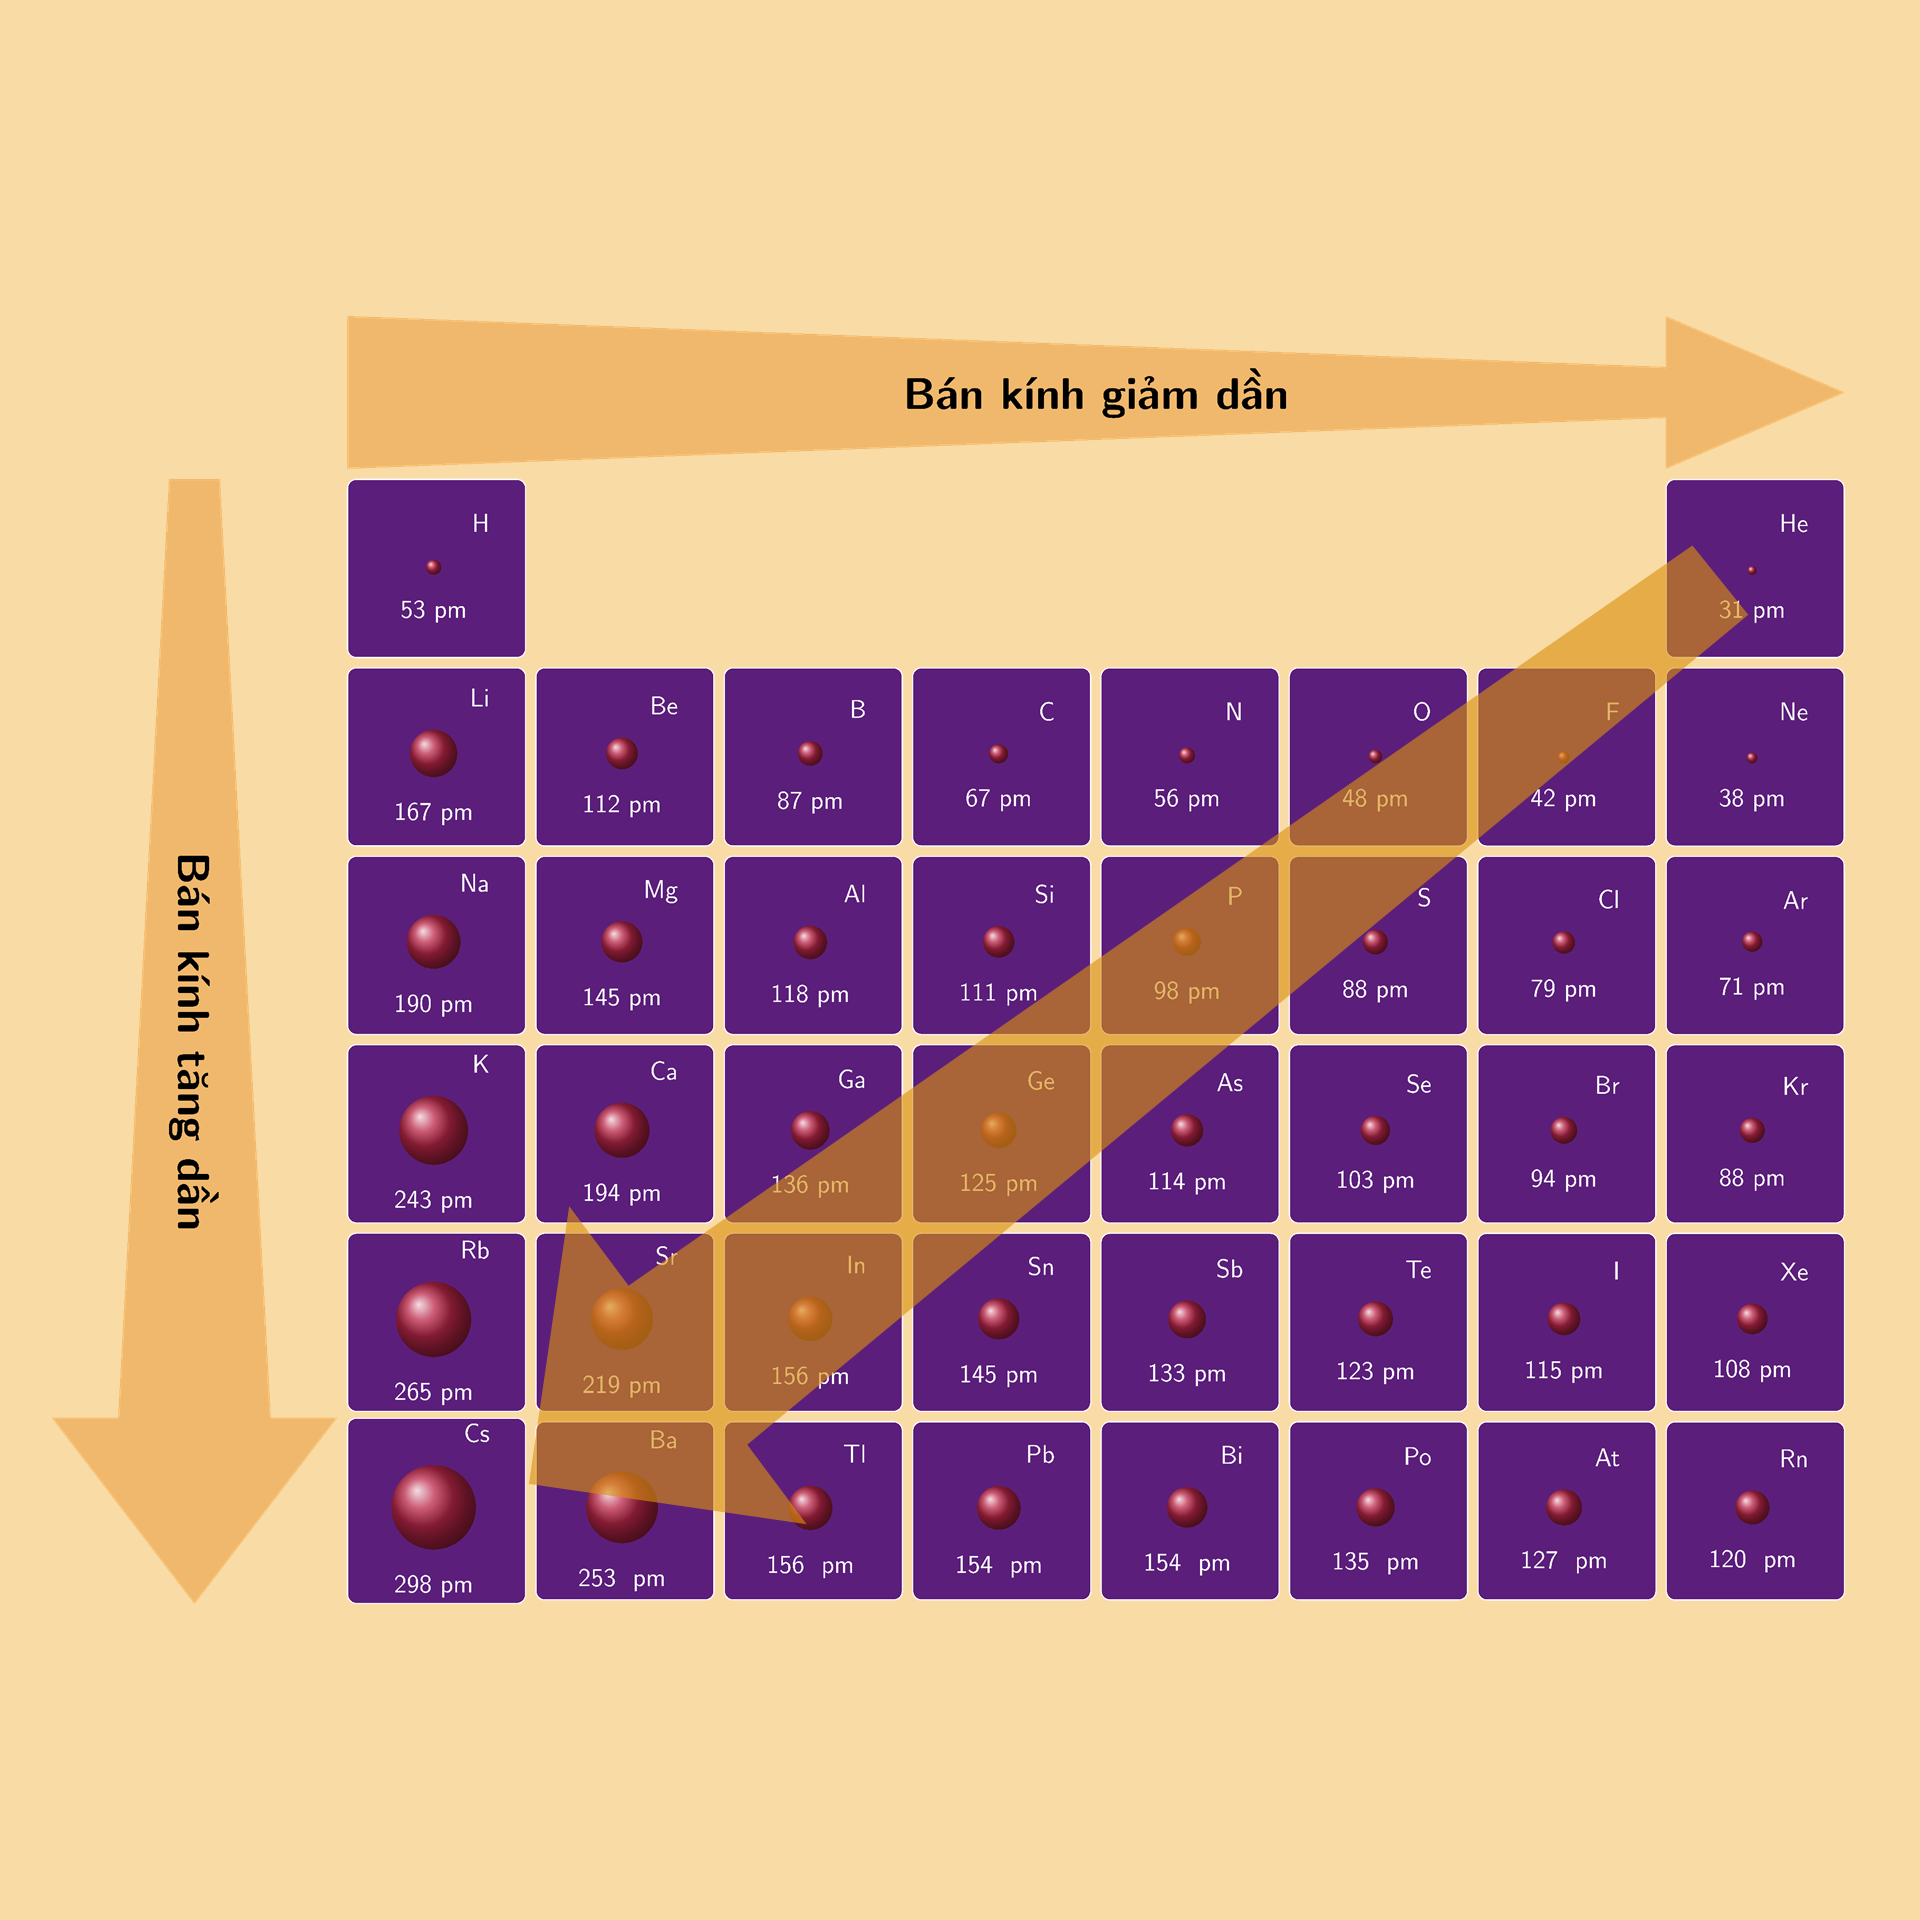
\includegraphics[width 	=8cm]{Images/anhminhoa/xuhuongbk.png}
	\end{center}
	\nhanmanh{Bài toán 2: So sánh bán kính ion}
	\GSND[\bfseries][\faBook][\maunhan]{Quy luât 1:}
%	\taodongke[\maunhan][1.12]{16}
	So với nguyên tử trung hòa
	\begin{enumerate}
		\item Khi một nguyên tử nhường e (cation) thì bán kính sẽ giảm đi
		\item Khi một nguyên tử nhận e (anion) thì bán kính nguyên tử sẽ tăng lên
	\end{enumerate}
	Do vây, đối với cùng nguyên tố thì:
	\begin{center}
		\boxct{Bán kính$_{cation}$ < bán kính $_{\text{nguyên tử}}$ < bán kính $_{anion}$}
	\end{center}
	\GSND[\bfseries][\faBook][\maunhan]{Quy luât 2:}
%	\taodongke[\maunhan][1.12]{18}
	Các ion có cùng số electron
	\begin{enumerate}
		\item Cation có điện tích càng lớn thì bán kính càng nhỏ
		\item Anion có điện tích càng lớn thì bán kính càng lớn
	\end{enumerate}
% \taodongke[\maunhan][1.12]{16}
\end{dangntd}
\newpage
\GSND[\bfseries][\faBookReader][\maudam]{Ví dụ mẫu:}
%%%==============VD_01===================%%%
\begin{vd}
	Hãy sắp xếp các nguyên tố $_{20}Ca$, $_{4}Be$, $_{12}Mg$ theo chiều tăng dần bán kính nguyên tử?
	\loigiai{
	Dựa vào  số hiệu nguyên tử các em viết cấu hình electron của các nguyên tử \Muiten{->} vị trí \Muiten{->} phác thảo lên bảng tuần hoàn  đưa ra quy luật biến đổi tính chất\\
	Ta có:\\
	$_{20}Ca: 1s^{2}2s^{2}2p^{6}3s^{2}3p^{6}4s^{2}$ \Muiten{->} Ca thuộc chu kì 4, nhóm IIA\\
	$_{4}Be: 1s^{2}2s^{2}$ \Muiten{->} Be thuộc chu kì 2, nhóm IIA\\
	$_{12}Mg: 1s^{2}2s^{2}2p^{6}3s^{2}$ \Muiten{->} Mg thuộc chu kì 3, nhóm IIA\\
	Ba nguyên tố Ca, Be, Mg thuộc cùng một nhóm nên chiều bán kính tăng dần là: Be < Mg < Ca
	}
\end{vd}
%%%==============VD_02===================%%%
\begin{vd}
	Hãy sắp xếp các nguyên tố $_{11}Na$, $_{17}Cl$, $_{15}P$, $_{13}Al$ theo chiều tăng dần bán kính nguyên tử?
	\sodongkevd[10]
\end{vd}
%%%==============VD_03===================%%%
\begin{vd}
	Hãy sắp xếp các nguyên tố $_{8}O$, $_{15}P$, $_{13}Al$, $_{20}Ca$, $_{19}K$ theo chiều tăng dần bán kính nguyên tử?
	\sodongkevd[10]
\end{vd}
%%%==============VD_04===================%%%
\begin{vd}
	Cho điện tích hạt nhân $O(Z=8), \mathrm{Na}(Z=11), \mathrm{Mg}(Z=12), \mathrm{Al}(Z=13)$ và các hạt vi mô: $O^{2-}, \mathrm{Al}^{3+}, \mathrm{Al}, \mathrm{Na}, \mathrm{Mg}^{2+}, \mathrm{Mg}$. Dãy nào sau đây được xếp đúng thứ tự bán kính hạt?
	\sodongkevd[15]
\end{vd}
%%%==============VD_05===================%%%
\begin{vd}
	Cho điện tích hạt nhân $O(Z=8), \mathrm{F}(Z=9), \mathrm{Mg}(Z=12), \mathrm{Al}(Z=13),\mathrm{S}(Z=16),\mathrm{Cl}(Z=17),\mathrm{K}(Z=19),\mathrm{Ca}(Z=20)$.Hãy sắp xếp dãy các ion sau: $\mathrm{S}^{2-},\mathrm{Cl}^{-},\mathrm{K}^{+},\mathrm{Ca}^{2+},\mathrm{Al}^{3+},\mathrm{Mg}^{2+},\mathrm{O}^{2-},\mathrm{F}^{-} $ theo chiều tăng dần của bán kính?
	\sodongkevd[15]
\end{vd}
%%%==========Nội dung file thứ 6===============%%%
\chapter{Liên kết hóa học}
\section{Quy tắc Octet}
\begin{mtbh}
	\begin{itemize}
		\item Trình bày được quy tắc octet với các nguyên tố nhóm $A$.
		\item Vận dụng được quy tắc octet trong quá trình hình thành liên kết hoá học ở các nguyên tố nhóm $A$.
	\end{itemize}
\end{mtbh}
\subsection{Kiến thức cần nhớ}
\begin{hoplythuyet}
	\GSND[\bfseries\sffamily][\faStar][\maunhan]{Liên kết hóa học:}
	Liên kết hóa học là sụ kết hợp giữa các nguyên tử tạo thành phân tử hay tinh thể bền vững hơn.
	\GSND[\bfseries\sffamily][\faStar][\maunhan]{Quy tắc octet:}
	Trong quá trình hình thành liên kết hóa học, nguyên tử của các nguyên tố nhóm A có xu hương tạo thành lớp vỏ ngoài cùng có 8 electron tương ứng với khí hiếm gần nhất (hoặc 2 electron với khí hiếm helium).
\end{hoplythuyet}
\begin{notegsnd}
	Không phải mọi trừờng hợp, nguyên tử của các nguyên tố khi tham gia liên kết đều tuân theo quy tắc octet. Người ta nhận thấy một số phân tủ không tuân theo quy tắc octet. Ví dụ: $\mathrm{NO}, \mathrm{BH}_3$, $S F_6, \ldots$
\end{notegsnd}

\columnratio{0.65}
\begin{paracol}{2}
	\begin{hoplythuyet}
		\GSND[\bfseries\sffamily][\faStar][\maunhan]{Liên kết hóa học:}
		Liên kết hóa học là sụ kết hợp giữa các nguyên tử tạo thành phân tử hay tinh thể bền vững hơn.
		\GSND[\bfseries\sffamily][\faStar][\maunhan]{Quy tắc octet:}
		Trong quá trình hình thành liên kết hóa học, nguyên tử của các nguyên tố nhóm A có xu hương tạo thành lớp vỏ ngoài cùng có 8 electron tương ứng với khí hiếm gần nhất (hoặc 2 electron với khí hiếm helium).
	\end{hoplythuyet}
	\switchcolumn 
	\begin{vdnote}
		Hai nguyên tử H liên kết với nhau tạo thành phân tử $H_2$ bền vững hơn nguyên tử H
	\end{vdnote}
	\begin{vdnote}
		Nguyên tử chlorine với cấu hình electron là $[\mathrm{Ne}] 3 \mathrm{~s}^2 3 \mathrm{p}^5$, có 7 electron ở lớp vỏ ngoài cùng.Khi hình thành liên kết hoá học chlorine nhận thêm 1 electron để đạt được lớp vỏ có 8 electron ở lớp ngoài cùng như của khí hiếm $\mathrm{Ar}$ (thay vì $\mathrm{Cl}$ phải nhường đi 7 electron để có lớp vỏ ngoài cùng là $2 \mathrm{~s}^2 2 \mathrm{p}^6$ - khó khăn hơn rất nhiều)
	\end{vdnote}
\end{paracol}

\newcommand{\ngoacvuongtron}[2][]{
	\begin{tikzpicture}[declare function={d=-4pt;},node distance=-d]
		\node (name) {#2};
		\node[anchor = base, above right =of name,shift={(-2pt,-5pt)}](plus) {$#1$};
		\draw[rounded corners=-d-1pt] (name.north west)--([xshift=d]name.north west)|-($(name.south west) +(0,0)$);
		\draw[rounded corners=-d-1pt] (name.north east)--([xshift=-d]name.north east)|-($(name.south east) +(0,0)$);
	\end{tikzpicture}
}
\newpage
\GSND[\bfseries\sffamily][\faStar][\maunhan]{Giải thích sự hình thành liên kết}
\columnratio{0.5}
\begin{paracol}{2}
	%%%================ Giải thích sự hình thành ion Cl ================%%%
	\begin{vdnote}
		Nguyên tử chlorine với cấu hình electron là $[Ne]3s^23p^5$, có 7 electron ở lớp ngoài cùng. Vậy có xu hướng nhận thêm 1 electron để đạt cấu hình bền vững giống khí hiếm Ar (hình \ref{ion_Cl})
	\end{vdnote}
	\begin{center}
		\begin{tikzpicture}[declare function ={k=5cm;},node distance=1.5cm]
			\node at (0:0) (Cl) {
				\begin{tikzpicture}[declare function={r=.5 cm;}]
					\tikzstyle{mystyle} = [draw=red,inner sep = 0pt,anchor=center, baseline]
					\path (0:0) coordinate (O);
					\fill[ball color=red!50](O) circle (r -.25 cm);
					\node[font=\tiny] at (O) {\textbf{+17}};
					\draw[mystyle] (O) circle (r+0.25cm);
					\foreach \g in {0,45,90,135,180,225,270,315}{\fill[ball color =\mauphu!50] (\g:{r+0.25cm}) circle (1pt);}
					\draw[mystyle] (O) circle (r+0.25*2cm);
					\foreach \g in {45,90,135,180,225,270,315}{\fill[ball color =\mauphu!50] (\g:{r+0.25*2cm}) circle (1pt);}
					\draw[mystyle] (O) circle (r);
					\foreach \g in {90,-90}{\fill[ball color =\mauphu!50] (\g:r) circle (1pt);}
				\end{tikzpicture}
			};
			\node[yshift=7pt] at (0:k)(ion-Cl) {
				\ngoacvuongtron[-]{\begin{tikzpicture}[declare function={r=.5 cm;},scale=1.2]
						\tikzstyle{mystyle} = [text centered, draw=red,inner sep = 0pt]
						\path (0:0) coordinate (O);
						\fill[ball color=red!50](O) circle (r -.25 cm);
						\node[font=\tiny] at (O) {\textbf{+17}};
						\draw[mystyle] (O) circle (r+0.25cm);
						\foreach \g in {0,45,90,135,180,225,270,315}{\fill[ball color =\mauphu!50] (\g:{r+0.25cm}) circle (1pt);}
						\draw[mystyle] (O) circle (r+0.25*2cm);
						\foreach \g in {0,45,90,135,180,225,270,315}{\fill[ball color =\mauphu!50] (\g:{r+0.25*2cm}) circle (1pt);}
						\draw[mystyle] (O) circle (r);
						\foreach \g in {90,-90}{\fill[ball color =\mauphu!50] (\g:r) circle (1pt);}
				\end{tikzpicture}}
			};
			\draw[-latex,line width=1pt] (Cl.east)--([yshift=-7pt]ion-Cl.west)node[midway,pos =0.5,above,font=\sf\small,yshift=-2pt]{nhận}node[midway,pos =0.5,below,font=\sf\small,yshift=2pt]{1 electron};
			\node [below of= Cl,font=\bfseries\small] {Cl};
			\node [below of= ion-Cl,font=\bfseries\small,shift={(-6pt,-9pt)}] {\text{Cl$^{-}$}};
		\end{tikzpicture}
		\captionof{figure}{Sơ đồ nguyên tử Cl nhận thêm 1 eclectron vào lớp ngoài cùng \label{ion_Cl}}
	\end{center}
	\switchcolumn
	%%%================Giải thích sự hình thành ion Na================%%%
	\begin{vdnote}
		Nguyên tử Sodium với cấu hình $[Ne]3s^1$, có 1 electron ở lớp ngoài cùng .Vậy xu hướng khi hình thành liên kết là nhường đi 1 electron để đạt được cấu hình electron giống khí hiếm Ne.(hình \ref{ion_Na})
	\end{vdnote}
	\begin{center}
		\begin{tikzpicture}[declare function ={k=5cm;},node distance=1.5cm]
			\node at (0:0) (Na) {
				\begin{tikzpicture}[declare function={r=.5 cm;}]
					\tikzstyle{mystyle} = [draw=red,inner sep = 0pt,anchor=center, baseline]
					\path (0:0) coordinate (O);
					\fill[ball color=red!50](O) circle (r -.25 cm);
					\node[font=\tiny] at (O) {\textbf{+11}};
					\draw[mystyle] (O) circle (r+0.25cm);
					\foreach \g in {0,45,90,135,180,225,270,315}{\fill[ball color =\mauphu!50] (\g:{r+0.25cm}) circle (1pt);}
					\draw[mystyle] (O) circle (r+0.25*2cm);
					\foreach \g in {0}{\fill[ball color =\mauphu!50] (\g:{r+0.25*2cm}) circle (1pt);}
					\draw[mystyle] (O) circle (r);
					\foreach \g in {90,-90}{\fill[ball color =\mauphu!50] (\g:r) circle (1pt);}
				\end{tikzpicture}
			};
			\node[yshift=7pt] at (0:k)(ion-Na) {
				\ngoacvuongtron[+]{\begin{tikzpicture}[declare function={r=.5 cm;},scale=1.2]
						\tikzstyle{mystyle} = [text centered, draw=red,inner sep = 0pt]
						\path (0:0) coordinate (O);
						\fill[ball color=red!50](O) circle (r -.25 cm);
						\node[font=\tiny] at (O) {\textbf{+11}};
						\draw[mystyle] (O) circle (r+0.25cm);
						\foreach \g in {0,45,90,135,180,225,270,315}{\fill[ball color =\mauphu!50] (\g:{r+0.25cm}) circle (1pt);}
						\draw[mystyle] (O) circle (r);
						\foreach \g in {90,-90}{\fill[ball color =\mauphu!50] (\g:r) circle (1pt);}
				\end{tikzpicture}}
			};
			\draw[-latex,line width=1pt] (Na.east)--([yshift=-7pt]ion-Na.west)node[midway,pos =0.5,above,font=\sf\small,yshift=-2pt]{nhường}node[midway,pos =0.5,below,font=\sf\small,yshift=2pt]{1 electron};
			\node [below of= Na,font=\bfseries\small] {Na};
			\node [below of= ion-Na,font=\bfseries\small,shift={(-6pt,-9pt)}] {\text{Na$^{+}$}};
		\end{tikzpicture}
		\captionof{figure}{Sơ đồ nguyên tử Na nhường đi 1 eclectron  \label{ion_Na}}
	\end{center}
\end{paracol}

\columnratio{0.5}
\begin{paracol}{2}
%%%================Giải thích sự hình thành phân tử H2================%%%		
	\begin{vdnote}
		Phân tử $\mathrm {H_2}$ được hình thành từ hai nguyên tử H bởi sự góp chung electron (hình \ref{hthidro})
	\end{vdnote}
	\begin{center}
		\tikzstyle{mystyle} = [draw=\mauphu!90!black,inner sep = 0pt,anchor=center, baseline,fill=\mauphu!90,opacity=.5,line width=.8pt]
		\begin{tikzpicture}[declare function ={k=1.8cm;},node distance=.5pt and .5pt]
			\node at (0:0) (H1) {
				\begin{tikzpicture}[declare function={r=.5 cm;}]
					\path (0:0) coordinate (O);
					\fill[ball color=\mauphu!90](O) circle (r -.25 cm);
					\node[font=\tiny] at (O) {\textbf{+1}};
					\filldraw[mystyle] (O) circle (r+0.25cm);
					\foreach \g in {25}{\fill[ball color =\mauphu!90] (\g:{r+0.25cm}) circle (1.5pt);}
				\end{tikzpicture}
			};
			\node [below=of H1]{\bf H};
			\node at (0:k)(H2) {
					\begin{tikzpicture}[declare function={r=.5 cm;}]
					\path (0:0) coordinate (O);
					\fill[ball color=\mauphu!90](O) circle (r -.25 cm);
					\node[font=\tiny] at (O) {\textbf{+1}};
					\filldraw[mystyle] (O) circle (r+0.25cm);
					\foreach \g in {205}{\fill[ball color =\mauphu!90] (\g:{r+0.25cm}) circle (1.5pt);}
				\end{tikzpicture}
			};
			\node [below=of H2]{\bf H};
			\node at (0:{3*k})(H3){
			\begin{tikzpicture}[declare function={r=.5 cm;}]
				\path (0:0) coordinate (O);
				\fill[ball color=\mauphu!90](O) circle (r -.25 cm);
				\node[font=\tiny] at (O) {\textbf{+1}};
				\filldraw[mystyle] (O) circle (r+0.25cm);
				\foreach \g in {-10}{\fill[ball color =\mauphu!90] (\g:{r+0.12cm}) circle (1.5pt);}
			\end{tikzpicture}
			};
			\node at (0:{3.68*k})(H4){
				\begin{tikzpicture}[declare function={r=.5 cm;}]
					\path (0:0) coordinate (O);
					\fill[ball color=\mauphu!90](O) circle (r -.25 cm);
					\node[font=\tiny] at (O) {\textbf{+1}};
					\filldraw[mystyle] (O) circle (r+0.25cm);
					\foreach \g in {170}{\fill[ball color =\mauphu!90] (\g:{r+0.12cm}) circle (1.5pt);}
				\end{tikzpicture}
			};
			\filldraw[-{Latex[length=5mm]},line width=6pt,draw=\mauphu,] (H2.east)--(H3.west) ;
			\node [below=of H3,xshift={.34*k}]{ $\mathbf {H_2}$};
		\end{tikzpicture}
		\captionof{figure}{Sự góp chung electron trong phân tử hiđro \label{hthidro}}
	\end{center}
		\switchcolumn
	%%%================Giải thích sự hình thành phân tử N2================%%%
	\begin{vdnote}
		Phân tử $\mathrm {N_2}$ được hình thành từ hai nguyên tử N bởi sự góp chung của 3 cặp electron (hình \ref{htnito})
	\end{vdnote}
	\begin{center}
		\tikzstyle{mystyle} = [draw=\mycolor!90!black,inner sep = 0pt,anchor=center, baseline,fill=\mycolor!90,opacity=.3,line width=.8pt]
		\begin{tikzpicture}[declare function ={k=2.5cm;R=1.2cm;},node distance=.5pt and .5pt]
			\node at (0:0) (N1) {
				\begin{tikzpicture}[declare function={r=.5 cm;}]
					\path (0:0) coordinate (O);
					\fill[ball color=\mycolor!90](O) circle (r -.25 cm);
					\node[font=\tiny] at (O) {\textbf{+7}};
					\filldraw[mystyle] (O) circle (r);
					\foreach \g in {90,-90}{\fill[ball color =\mycolor!70] (\g:{r}) circle (1.5pt);}
					\filldraw[mystyle] (O) circle (r+0.25cm);
					\foreach \g in {170,-170,45,-45,0}{\fill[ball color =\mycolor!90] (\g:{r+0.25cm}) circle (1.5pt);}
				\end{tikzpicture}
			};
%	
			\node at (0:.5*k) (plus){\large +};
			\node at (0:k) (N2) {
				\begin{tikzpicture}[declare function={r=.5 cm;}]
					\path (0:0) coordinate (O);
					\fill[ball color=\mycolor!90](O) circle (r -.25 cm);
					\node[font=\tiny] at (O) {\textbf{+7}};
				\begin{scope}[transform canvas={xscale=-1}]
					\filldraw[mystyle] (O) circle (r);
					\foreach \g in {90,-90}{\fill[ball color =\mycolor!70] (\g:{r}) circle (1.5pt);}
					\filldraw[mystyle] (O) circle (r+0.25cm);
					\foreach \g in {170,-170,45,-45,0}{\fill[ball color =\mycolor!90] (\g:{r+0.25cm}) circle (1.5pt);}
				\end{scope}
				\end{tikzpicture}
			};
			
			\node at (0:{2.4*k}) (N3) {
				\begin{tikzpicture}[declare function={r=.5 cm;}]
					\path (0:0) coordinate (O);
					\fill[ball color=\mycolor!90](O) circle (r -.25 cm);
					\node[font=\tiny] at (O) {\textbf{+7}};
					\begin{scope}[transform canvas={xscale=1}]
						\filldraw[mystyle] (O) circle (r);
						\foreach \g in {90,-90}{\fill[ball color =\mycolor!70] (\g:{r}) circle (1.5pt);}
						\filldraw[mystyle] (O) circle (r+0.25cm);
						\foreach \g in {170,-170}{\fill[ball color =\mycolor!90] (\g:{r+0.25cm}) circle (1.5pt);}
					\end{scope}
				\end{tikzpicture}
			};
				\node at (0:{2.90*k}) (N4) {
				\begin{tikzpicture}[declare function={r=.5 cm;}]
					\path (0:0) coordinate (O);
					\fill[ball color=\mycolor!90](O) circle (r -.25 cm);
					\node[font=\tiny] at (O) {\textbf{+7}};
					\begin{scope}[transform canvas={xscale=-1}]
						\filldraw[mystyle] (O) circle (r);
						\foreach \g in {90,-90}{\fill[ball color =\mycolor!70] (\g:{r}) circle (1.5pt);}
						\filldraw[mystyle] (O) circle (r+0.25cm);
						\foreach \g in {170,-170}{\fill[ball color =\mycolor!90] (\g:{r+0.25cm}) circle (1.5pt);}
					\end{scope}
				\end{tikzpicture}
			};
			\node at (0:{2.4*k+.56cm}) {\tikz{\fill[ball color =\mycolor!90]circle (1.45pt);}};
			\node at (0:{2.4*k+.7cm}) {\tikz{\fill[ball color =\mycolor!90]circle (1.45pt);}};
			\node at ([yshift=4pt]0:{2.4*k+.57cm}) {\tikz{\fill[ball color =\mycolor!90]circle (1.45pt);}};
			\node at ([yshift=4pt]0:{2.4*k+.68cm}) {\tikz{\fill[ball color =\mycolor!90]circle (1.45pt);}};
			\node at ([yshift=-4pt]0:{2.4*k+.57cm}) {\tikz{\fill[ball color =\mycolor!90]circle (1.45pt);}};
			\node at ([yshift=-4pt]0:{2.4*k+.68cm}) {\tikz{\fill[ball color =\mycolor!90]circle (1.45pt);}};
			\filldraw[-{Latex[length=5mm]},line width=6pt,draw=\mycolor,] ([xshift=.5cm]N2.east)--([xshift=-.5cm]N3.west) ;
			\node at ([yshift=-4pt]0:{2.4*k+.68cm}) {\tikz{\fill[ball color =\mycolor!90]circle (1.45pt);}};
			\node at ([yshift=-R]0:0) {\large N};
			\node at ([yshift=-R]0:{k}) {\large N};
			\node at ([yshift=-R]0:{2.65*k}) {\large $\mathbf{N_2}$};
		\end{tikzpicture}
		\captionof{figure}{Sự góp chung electron trong phân tử nitơ \label{htnito}}
	\end{center}
\end{paracol}
\subsection{Bài tập}
%%%===============Câu_01=======================%%%		
\begin{ex}[][Quy tắc octet]
	Biết phân tử magnesium được hình thành từ các ion $Mg^{2+}$ và ion $O^{2-}$.Vận dụng quy tắc octet, trình bày sự hình thành các ion trên từ những nguyên tử tương ứng.
	\huongdan{
	\begin{itemize}
		\item Mg (Z=12):$1s^22s^22p^63s^2$ (có 2 electron ở lớp ngoài cùng) $\Rightarrow$ $Mg \longrightarrow$ $Mg^{2+} + 2e$
		\item O (Z=8):$1s^22s^2p^4$ (có 6 electron ở lớp ngoài cùng) $\Rightarrow$ $O + 2e \longrightarrow$ $O^{2-} $
	\end{itemize}
	
	}
\end{ex}
%%%===============Câu_02=======================%%%		
\begin{ex}[][Quy tắc octet]
	Cho các nguyên tử của các nguyên tố sau:Na(Z=11), Cl(Z=17), Ne(Z=10), Ar(Z=18).Những nguyên tử nào trong các nguyên tử trên có lớp electron bền vững.
	\huongdan{
		\begin{multicols}{2}
			\begin{itemize}
			\item Na (Z=11):$1s^22s^22p^63s^1$ 
			\item Cl (Z=17):$ 1s^22s^22p^63s^23p^5$
			\item Ne (Z=10):$ 1s^22s^22p^6$
			\item Ar (Z=18):$ 1s^22s^22p^63s^23p^6$
		\end{itemize}
		\end{multicols}
	}
\end{ex}















%\newpage
%\setchemfig{%
%	atom sep= 2em,
%	bond offset=2pt,
%	compound sep=5em
%}

%\schemestart
%\chemname{\chemfig{
%H-@{N}\charge{0:2pt=\:}{N}(-[6]H)-[2]H
%}}{\scriptsize\quad\quad Ammonia\vphantom{aa}}
%\+
%\chemfig{
%@{H}\charge{45:3pt=$\scriptstyle+$}{H}
%}
%\arrow(.mid east--.mid west)[,.7,-latex]
%\chemname{\ngoacvuongtron{\chemfig{
%			H-N(-[2]H)(-[6]H)-[,,,,-stealth]H
%}}}{\scriptsize Ammonium\quad}
%\schemestop
%
%\chemmove[shorten <=4pt,shorten >=4pt,-latex] {
%\draw ([shift={(-25:3.5pt)}]N.25).. controls +(80:8mm) and +(100:8mm)..([shift={(29:3.5pt)}]H.65)
%;}
%%%%=============Tinh thể NaCl===================%%%
%\begin{tikzpicture}[node distance=0pt]
%	% Định dạng cho cột của bảng
%	\tikzset{%
%		%% Định dạng ô
%		mynode/.style={%
%			circle,
%			ultra thin,
%			minimum height=0.65cm,
%			minimum width=0.65cm,
%			align=center
%		},
%		mymatrix/.style={%
%			matrix of nodes,
%			ampersand replacement=\&,
%			inner sep =5pt,
%			nodes in empty cells,
%			fill =\mycolor!15,
%			row sep=-3-\pgflinewidth,
%			column sep=-3-\pgflinewidth,
%			nodes={mynode}
%		}
%	}
%	\matrix(Bang)[mymatrix]{%
%	\&\&\&\&\&\\
%	\&\&\&\&\&\\
%	\&\&\&\&\&\\
%	\&\&\&\&\&\\
%	\&\&\&\&\&\\
%	};
%\foreach \x in {1,3,5}{
%	\foreach \y in {1,3,5}{
%	\fill [ball color=\maunhan!70 ] (Bang-\x-\y) circle (0.3cm) node[font=\tiny\sffamily\bfseries\color{white}](Na) {Na} ;
%	\node [font=\fontsize{5pt}{3pt}\selectfont\sffamily\bfseries\color{white}] at ([shift={(60:4.8pt)}]Bang-\x-\y) {+};
%	}
%}
%\foreach \x in {2,4}{
%	\foreach \y in {2,4,6}{
%		\fill [ball color=\maunhan!70 ] (Bang-\x-\y) circle (0.3cm);
%	}
%}
%\foreach \x in {1,3,5}{
%	\foreach \y in {2,4,6}{
%		\fill [ball color=\maudam!70 ] (Bang-\x-\y) circle (0.2cm);
%	}
%}
%\foreach \x in {2,4}{
%	\foreach \y in {1,3,5}{
%		\fill [ball color=\maudam!70 ] (Bang-\x-\y) circle (0.2cm);
%	}
%}
%\end{tikzpicture}
%%%==========Nội dung file thứ 7===============%%%
\newenvironment{cacbuoc}{\begin{enumerate}[label= \color{\maunhan}\bfseries\fontfamily{qag}\selectfont{\faAdjust\;Bước \arabic*:},itemsep=0pt,wide=0cm,leftmargin=0.5cm,topsep=0pt]
	}{\end{enumerate}}
\newtcolorbox{body}{%
	enhanced,
	before skip=1cm,
	breakable,
	colback=\mycolor!20,
	enhanced jigsaw,opacityback=0,opacitybacktitle=0,
	opacityback=0,
	colframe=\mycolor
}
\renewcommand{\thesubsubsection}{\Roman{subsubsection}}
\titlespacing*{\subsection}{3pt}{0pt}{-5pt}
\titlespacing*{\subsubsection}{3pt}{5pt}{-5pt}
\titlespacing*{\paragraph}{0cm}{0cm}{-5pt}
\setcounter{chapter}{3}
\chapter{Phản ứng Oxi hóa - khử}
\section{Số Oxi hóa - Cân bằng phản ứng oxi hóa khử}
\subsection{Kiến thức cần nhớ}
\begin{body}
	\subsubsection{Số oxi hóa}
	\begin{dn}
		\indam{Số oxi hóa} của một nguyên tử một nguyên tố trong hơp chất là \indam{điện tích} của nguyên tử nguyên tố đó với giả định đây là hợp chất ion.
	\end{dn}
	\subsubsection{Cách xác định số oxi - hóa}
	\begin{enumerate}
		\item \indam{Quy tắc 1:}
		Trong đơn chất, số oxi hóa của các nguyên tố bằng 0.\\
		VD: $\overset{0}{\mathrm{H}_{2}}$, $\overset{0}{\mathrm{Na}}$, $\overset{0}{\mathrm{O}_{3}}$, $\ldots$
		\item \indam{Quy tắc 2:}
		Trong một phân tử,tổng số oxi hóa  của các nguyên tố nhân với số nguyên tử của từng nguyên tố bằng 0\\
		\item \indam{Quy tắc 3:} 
		\begin{itemize}
			\item Trong các ion \indam{đơn nguyên tử}, số oxi hóa của các nguyên tố bằng điệnu tích của ion đó\\
			\item Trong ion \indam{đa nguyên tử}, tổng số oxi hóa các nguyên tố nhân với số nguyên tử của từng nguyên tố bằng điện tích của ion
		\end{itemize}
		\item \indam{Quy tắc 4:} \\
		\begin{itemize}
			\item Trong đa số các hợp chất, số oxi hóa của hydrogen bằng +1 , trừ hydride kim loại ($NaH$, $CaH_2$)\\
			\item Số oxi hóa của oxygen bằng $-\mathrm{2}$, trừ trường hợp $\overset{+1}{\mathrm{O}_{}}\overset{\vphantom{-1}}{\mathrm{F}_{2}}$ và peoxit $\left(\overset{\vphantom{+1}}{\mathrm{Na}_{2}}\overset{-1}{\mathrm{O}_{2}}\right)$, superoxide $\left(\overset{\vphantom{+1}}{\mathrm{K}_{}}\overset{-\tfrac{1}{2}}{\mathrm{O}_{2}}, \ldots\right)$.\\
			\item Các nguyên tố nhóm IA, IIA luôn có số oxi hóa $+1,+2$, số oxi hóa của $\mathrm{Al}$ là +3 . Số oxi hóa của nguyên tử nguyên tố fluorine trong các hợp chất bằng -1
		\end{itemize}
	\end{enumerate}
	\subsubsection{Phản ứng Oxi hóa - khử}
	\paragraph{Sự oxi hóa-sự khử}
	\begin{mylt}
		\begin{enumerate}[label = \indam{\alph*)}]
			\item \indam{Sự oxi hóa} là sự nhường electron, là sự tăng số oxi hóa.\\
			\indam{Ví dụ:} $\overset{0}{Mg} \rightarrow Mg^{2+} + 2e$
			\item \indam{Sự khử} là sự thu electron, là sự giảm electron.\\
			\indam{Ví dụ:} $Cu^{2+} +2e \rightarrow Cu $
		\end{enumerate}
	\end{mylt}
	\paragraph{Chất oxi hóa - chất khử}
	\begin{mylt}
		\begin{enumerate}[label = \indam{\alph*)}]
			\item \indam{Chất oxi hóa} là chất thu electron.là chất chứa nguyên tố có số oxi hóa giảm sau phản ứng.\\
			\indam{Chất oxihóa} còn gọi là chất \indam{bị khử}.
			\item \indam{Chất khử} là chất nhường electron, là chất có số oxi hóa tăng sau phản ứng\\
			\indam{Chất khử} còn gọi là chất \indam{bị oxi hóa}.
		\end{enumerate}
	\end{mylt}
	\begin{vdnote}
		$ \overset{0}{Mg} + \overset{+2}{Cu}SO_{4} \rightarrow\overset{+2}{Mg}SO_{4}  + \overset{0}{Cu}$.\\
		$Cu^{2+}$ nhận electron, là chất oxi hóa ( số oxi hóa giảm từ +2 về 0).
		$Mg$ nhường electron, là chất khử (số oxi hóa tăng từ 0 lên +2)
	\end{vdnote}
	\begin{vdnote}
		$\overset{+3}{Fe_2}\overset{\vphantom{+3}}{O_3} + 3\overset{+2}{C}O$ $\longrightarrow$ $ 2 \overset{0}{Fe} + 3\overset{+4}{C}O_2$
	\end{vdnote}
	\paragraph{Phản ứng Oxi hóa - khử }
	\begin{mylt}
		\indam{Phản ứng oxi - hóa khử } là phản ứng hóa học trong đó có sự chuyển electron giữa các chất phản ứng.\\
		Nếu dựa vào sự thay đổi số oxi hóa thì phản ứng oxi hóa-khử là phản ứng hóa học trong đó có sự  thay đổi số oxi hóa của một số nguyên tố.\\
		
		\begin{vdnote}
			\[\begin{tikzpicture}
				\tikzstyle{mynode} =[
				font=\normalsize,
				line width =.8pt,
				anchor=center,
				align =center,
				]
				%%%==================%%%
				\tikzstyle{mymatrix} = [
				matrix of nodes,
				nodes in empty cells,
				nodes={mynode},
				column sep=-\pgflinewidth,
				row sep = -\pgflinewidth,
				minimum width = .5cm,
				minimum height = .6cm,
				column 4/.style={
					minimum width = .7cm,
				},
				]
				%%%=======================================================%%%
				\matrix(m) [mymatrix]{
					Mg & + & $CuSO_4$ & [-.7cm]\muiten[][][0.7]{->}& $MgSO_4$ & + & Cu\\
				};
				\node(0)[yshift=4pt,\maunhan] at (m-1-1.north){0};
				\node(2)[xshift =-8pt,yshift=4pt,\maunhan] at (m-1-3.north){+2};
				\node[xshift =-8pt,yshift=4pt,\maunhan] at (m-1-5.north){+2};
				\node[yshift=4pt,\maunhan] at (m-1-7.north){0};
				\draw[->,>=stealth,violet,ultra thick](0.90)--++(90:.5cm)-|(2.90) ;
				\path ($(0.90)+(90:.5cm)$)-- ($(2.90)+(90:.5cm)$) node [pos=.5,above,violet]{- 2 e};
			\end{tikzpicture}\]
			Trong phản ứng trên $Mg$ nhường đi 2 electron cho ion $Cu^{+2}$ trở thành ion $Mg^{+2}$ và ion $Cu^{+2}$ nhận  2 electron từ nguyên tử $Mg$ trở thành nguyên tử Cu.
		\end{vdnote}
		%%%===============Môi Trường Matrix=================%%%
	\end{mylt}
	\subsubsection{Cân bằng phản ứng oxi hóa-khử}
	\begin{mylt}
		\GSND[\bfseries\sffamily][\faStar]{Phương pháp thăng bằng electron:}\\
		Phương pháp này dựa trên nguyên tắc:
		\boxct[\mauphu][3pt][\bfseries\sffamily\color{violet}]{Tổng số electron chất khử nhường  = tổng số electron mà chất oxi hóa nhận}
		\indam{\faBook\ Các bước cân bằng:}\vspace{.5cm}
		\begin{vdnote}
			Lập phương trình phản ứng Oxi hóa - khử sau: 
			\[\puhh[$t^{\circ}$]{$Cu$\+ $HNO_3$}{->}{$Cu({NO_3})_2$ \+ $NO\uparrow$ \+ $H_2O$}\]
		\end{vdnote}
		\indam{\itshape Hướng dẫn giải:}
		\begin{cacbuoc}
			\item Xác định số oxi hóa của nguyên tử cóa sự thay đổi số oxi hóa, xác định chất khử, chất oxi hóa
			\[\begin{tikzpicture}
				\tikzstyle{mynode} =[
				font=\normalsize,
				line width =.8pt,
				anchor=center,
				align =center,
				]
				%%%==================%%%
				\tikzstyle{mymatrix} = [
				matrix of nodes,
				nodes in empty cells,
				nodes={mynode},
				column sep=-\pgflinewidth,
				row sep = -\pgflinewidth,
				minimum width = .5cm,
				minimum height = .6cm,
				column 4/.style={
					minimum width = .7cm,
				},
				]
				%%%=======================================================%%%
				\matrix(m) [mymatrix]{
					$Cu$ & + & $HNO_3$ & [-.7cm]\muiten[][][0.7]{->}& $Cu({NO_3})_{2}$ & + & $NO\uparrow$ & + & $H_2O$ \\
				};
				\node(0)[yshift=4pt,\maunhan] at (m-1-1.north){0};
				\node(chatkhu)[yshift=-4pt,\maunhan,font=\footnotesize] at (m-1-1.south){(Chất khử)};
				\node(2)[xshift =-2pt,yshift=4pt,\maunhan] at (m-1-3.north){+5};
				\node(chatoxh)[yshift=-4pt,\maunhan,font=\footnotesize] at (m-1-3.south){(Chất oxi hóa)};
				\node[xshift =-18pt,yshift=4pt,\maunhan] at (m-1-5.north){+3};
				\node[xshift =-8pt,yshift=4pt,\maunhan] at (m-1-7.north){+2};
			\end{tikzpicture}\]
			\item Viết quá trình oxi hóa và quá trình khử
			\[\begin{tikzpicture}
				\tikzstyle{mynode} =[
				font=\normalsize,
				line width =.8pt,
				anchor=center,
				align =center,
				minimum width = 0.4cm,
				minimum height = 1.0cm,
				]
				%%%==================%%%
				\tikzstyle{mymatrix} = [
				matrix of nodes,
				nodes in empty cells,
				nodes={mynode},
				column sep=-\pgflinewidth,
				row sep = 2pt-\pgflinewidth,
				column 1/.style={
					minimum width = 4cm,
					anchor =east,
					align =center,
				},
				]
				%%%=======================================================%%%
				\matrix(m) [mymatrix]{
					\text{Quá trình oxi hóa :} & Cu & [-.5cm]\muiten[][][0.4]{->}& Cu & + & 2e\\
					\text{Quá trình khử :} & N & + & [-.5cm]3e & [-.5cm]\muiten[][][0.4]{->} & NO\\
				};
				\node(0)[yshift=-2pt,\maunhan] at (m-1-2.north){0};
				\node(3)[yshift=-2pt,\maunhan] at (m-1-4.north){+2};
				\node(5)[yshift=-2pt,\maunhan] at (m-2-2.north){+5};
				\node(2)[xshift=-2pt,yshift=-2pt,\maunhan] at (m-2-6.north){+2};
			\end{tikzpicture}\]
			\item Nhân hệ số thích hợp  vào các quá trình  sao cho tổng  số electron chất khử nhường  bằng tổng số electron chất oxi hóa nhận.
			\[\begin{tikzpicture}
				\tikzstyle{mynode} =[
				font=\normalsize,
				line width =.8pt,
				anchor=center,
				align =center,
				minimum width = 0.4cm,
				minimum height = 1.0cm,
				]
				%%%==================%%%
				\tikzstyle{mymatrix} = [
				matrix of nodes,
				nodes in empty cells,
				nodes={mynode},
				column sep=3pt-\pgflinewidth,
				row sep = 2pt-\pgflinewidth,
				column 1/.style={
					minimum width = 4cm,
					anchor =east,
					align =center,
				},
				]
				%%%=======================================================%%%
				\matrix(m) [mymatrix]{
					3 x & Cu & [-.5cm]\muiten[][][0.4]{->}& Cu & + & 2e\\
					2 x & N & + & [-.5cm]3e & [-.5cm]\muiten[][][0.4]{->} & NO\\
				};
				\node(0)[yshift=-2pt,\maunhan] at (m-1-2.north){0};
				\node(3)[yshift=-2pt,\maunhan] at (m-1-4.north){+2};
				\node(5)[yshift=-2pt,\maunhan] at (m-2-2.north){+5};
				\node(2)[xshift=-2pt,yshift=-2pt,\maunhan] at (m-2-6.north){+2};
				\draw[\maunhan,line width=1pt] (m-1-1.north east)--(m-2-1.south east);
			\end{tikzpicture}\]
			\item Đặt các hệ số vào sơ đồ phản ứng. Can bằng số lượng  nguyên tử của các nguyên tố còn lại.
			\[\puhh[$t^{\circ}$]{$3Cu$ \+ ${8HNO_3}_{\text{loãng}}$}{->}{$3Cu({NO_3})_{2}$ \+ $2NO$ \+ $4H_2O$}\]
		\end{cacbuoc}
	\end{mylt}
\end{body}
\newpage
\subsection{Các dạng bài tập}
\begin{dangNTD}{Câu hỏi lý thuyết về phản ứng oxi hóa khử}
\end{dangNTD}
\begin{vdm}
\end{vdm}

\hienthiloigiaivd
%%%=========vd_1=========%%%
\begin{vd}[1][Nhận biết các quá trình vai trò của các chất]Một nguyên tử nhôm (Al) chuyển thành ion $Al^{3+}$ thực hiện :
	\choice
	{%
		nhận thêm 3 electron (quá trình oxi hóa)
	}{%
		nhường đi 3 electron (quá trình khử)
	}{%
		nhận thêm 3 electron (quá trình khử)
	}{%
		\True nhường đi 3 electron (quá trình oxi hóa)
	}
	\loigiai{Quá trình oxi hóa  một chất là làm cho nguyên tử trong chất đó nhường electron hay làm tăng số oxi hóa của nguyên tử trong chất đó.\\
		Quá trình khử  một chất là làm cho nguyên tử trong chất đó nhận electron hay làm giảm số oxi hóa của nguyên tử trong chất đó.\\
		Ta thấy số oxi hóa của nhôm tăng (quá trình oxi hóa) \\
		$\begin{matrix}
			\overset{0}{Al}& \muiten[][][.4]{->} &\overset{+3}{Al} & + & 3e
		\end{matrix}$
	}
\end{vd}
%%%=========vd_2=========%%%
\begin{vd}[2][Nhận biết các quá trình vai trò của các chất]Trong phản ứng : \puhh{$Cl_2$\+ $2KBr$}{->}{$Br_2$\+ 2KCl}, $Cl_2$ đóng vai trò 
	\choice{%
		\True là chất oxi hóa
	}{%
		là chất khử
	}{%
		không bị oxi hóa, không bị khử
	}{%
		vừa bị oxi hóa, vừa bị khử.
	}
	\loigiai{Chất oxi hóa là chất nhận electron hay là chất có số oxi hóa giảm sau phản ứng.\\
		Chất khử là chất nhường electron hay là chất có số oxi hóa tăng sau phản ứng.\\
		Ta thấy số oxi hóa của Cl giảm :\\
		$\begin{matrix}
			Cl_2 & + & 2e & \muiten[][][.4]{->} & 2Cl^{-}
		\end{matrix}$
	}
\end{vd}

%%%=========vd_3=========%%%
\begin{vd}[2][Nhận biết phản ứng oxi hóa khử]
	Phản ứng nào sau đây \indam[black]{không phải} phản ứng oxi hóa khử
	\choice{
		\puhh{$2NaOH$\+ $Cl_2$}{->}{$NaCl$\+$NaClO$\+ $H_2O$}
	}{
		\True \puhh[$t^{\circ}$]{$CaCO_3$}{->}{$CaO$\+$CO_2$}
	}{
		\puhh[$t^{\circ}$]{$2KClO_3$}{->}{$2KCl$\+$3O_2$}
	}{
		\puhh{$Fe$\+ $2HCl$}{->}{$FeCl_2$\+$H_2$}
	}
	\loigiai{%
		Phản ứng oxi hóa - khử là phản ứng  hóa học trong đó có sự thay đổi số oxi hóa.\\
		Phản ứng không phải là phản ứng oxi hóa - khử là phản ứng không có sự thay đổi số oxi hóa của các nguyên tố\\
		Ta có:\\
		$\begin{matrix}
			2NaOH  & + & \overset{0}{Cl}_{2} & \muiten{->} & \overset{\vphantom{+1}}{Na}\overset{-1}{Cl} & + & \overset{\vphantom{+1}}{Na}\overset{+1}{Cl}O  & + & H_2O\\
		\end{matrix}$\\
		$\begin{matrix}
			\overset{\vphantom{+4}}{Ca}\overset{+4}{C}\overset{\vphantom{-2}}{O_3} & \muiten{->}& \overset{+2}{Ca}O & + & \overset{+4}{C}\overset{\vphantom{+4}}{O_2}\\
		\end{matrix}$\\
		$\begin{matrix}
			\overset{\vphantom{-2}}{2K}\overset{+5}{Cl}\overset{\vphantom{-2}}{O_3} & \muiten{->}& \overset{\vphantom{-2}}{2K}\overset{-1}{Cl} & + & 3\overset{-2}{O_2}\\
		\end{matrix}$\\
		$\begin{matrix}
			\overset{0}{Fe}& + & 2\overset{+1}{H}Cl & \muiten{->}& \overset{+2}{Fe}\overset{\vphantom{-2}}{Cl_2} & + & \overset{0}{H_2} \\
		\end{matrix}$\\
		\indam{Nhận xét: }Phản ứng B không có sự thay đổi số oxi hóa của các nguyên tố. $\longrightarrow$ Phản ứng B không phải là phản ứng oxi hóa - khử
	}
\end{vd}


%%%=========vd_4=========%%%
\begin{vd}[2][Nhận biết phản ứng oxi hóa khử]Cho các phản ứng sau đây:
	\begin{enumerate}[a)]
		\item $C + O_{2} \xrightarrow{t^{\circ}} CO_{2}$
		\item $CaO +  H_{2}O \longrightarrow Ca(OH)_{2}$
		\item $CuO + H_{2} \xrightarrow{t^{\circ}} Cu + O_2$
		\item $2KMnO_4 \xrightarrow{t^{\circ}} K_2MnO_4 + MnO_2 + H_2O$
		\item $Cl_2 + 2KOH \longrightarrow KCl + KClO + H_2O$
		\item $Fe_3O_4 + 8HCl \longrightarrow 2FeCl_3 + FeCl_2 + 4H_2O$
	\end{enumerate}
	Số phản ứng thuộc loại phản ứng oxi hóa - khử là:
	\choice{2}{\True 4}{3}{5}
	\loigiai{%
		Phản ứng oxi hóa khử là phản ứng hóa học trong đó có sự thay đổi số oxi hóa của một số nguyên tố.
		\begin{enumerate}[a)]
			\item $\overset{0}{C} + \overset{0}{O}_{2} \xrightarrow{t^{\circ}} \overset{+4}{C}\overset{-2}{O}_{2}$
			\item $\overset{+2}{Ca}\overset{-2}{O} +  \overset{+1}{H_{2}}\overset{-2}{O} \longrightarrow \overset{+2}{Ca}(\overset{-2}{O}\overset{+1}{H})_{2}$
			\item $\overset{+2}{Cu}\overset{-2}{O} + \overset{-2}{H}_{2} \xrightarrow{t^{\circ}} \overset{0}{Cu} + \overset{+1}{H}_2\overset{-2}{O}$
			\item $2K\overset{+7}{Mn}\overset{-2}{O}_4 \xrightarrow{t^{\circ}} K_2\overset{+6}{Mn}O_4 + \overset{0}{O}_2 + \overset{+6}{Mn}O_{2}$
			\item $\overset{0}{Cl}_2 + 2KOH \longrightarrow K\overset{-1}{Cl} + K\overset{+1}{Cl}O + H_2O$
			\item $\overset{+8/3}{Fe_3}\overset{-2}{O_4} + 8\overset{+1}{H}\overset{-1}{Cl} \longrightarrow 2\overset{+3}{Fe}Cl_3 + \overset{+2}{Fe}\overset{-1}{Cl}_2 + 4\overset{+1}{H}_2O$
		\end{enumerate}
		\indam{Nhận xét:} Phản ứng a), c), d), e) có sự thay đổi số oxi hóa của các nguyên tố. $\Rightarrow$ Phản ứng a), c), d), e) là phản ứng oxi hóa - khử 
	}
\end{vd}
%%%=========vd_5=========%%%
\begin{vd}[2][Cân bằng phản ứng oxi hóa khử]Lập phương trình phản ứng oxi hóa - khử sau đây:
	\puhh{ $MnO_2$ \+ $HCl$}{->}{$MnCl_2$ \+ $ Cl_2$ \+ $H_2O$}
	\loigiai{\begin{cacbuoc}
			\item Xác định số oxi hóa của các nguyên tố :\\
			$\overset{+4}{Mn}O_2 + H\overset{-1}{Cl} \longrightarrow \overset{+2}{Mn}Cl_2 + \overset{0}{Cl_2} + H_2O$ 
			\item Quá trình cho - nhận electron\\
			$\begin{matrix}
				2\overset{-1}{Cl} & \longrightarrow& Cl_2 & + & 2e\\
				\overset{+4}{Mn} &  + & 2e & \longrightarrow & \overset{+2}{Mn}
			\end{matrix}$
			\item Đặt hệ số \\
			$\begin{matrix}
				1x|~2\overset{-1}{Cl} & \longrightarrow& Cl_2 & + & 2e\\
				1x|~\overset{+4}{Mn} &  + & 2e & \longrightarrow & \overset{+2}{Mn}
			\end{matrix}$
			\item Phương trình hóa học
			\boxct{$MnO_2 + 4HCl \longrightarrow MnCl_2 + Cl_2 + 2H_2O$}
	\end{cacbuoc}}
\end{vd}
%%%=========vd_6=========%%%
%%%==========================%%%
%%%==========================%%%
\begin{vd}[3][Cân bằng phản ứng oxi hóa - khử][Nguồn:CĐA 2010] Cho phản ứng:
	$\mathrm{Na}_2 SO_3+\mathrm{KMnO}_4+\mathrm{NaHSO}_4 \to \mathrm{Na}_2 SO_4+\mathrm{MnSO}_4+K_2 SO_4+H_2 O$.Tổng hệ số của các chất (là những số nguyên, tối giản) trong phương trình phản ứng là
	\choice
	{23}
	{27}
	{47}
	{31}
	\loigiai{
		\begin{cacbuoc}
			\item Xác định số oxi hóa của các nguyên tố :\\
			$Na_2\overset{+4}{S}O_3$ + $K\overset{+7}{Mn}O_4$ + $NaHSO_4$ $\to$ $Na_2\overset{+6}{S}O_4$ + $\overset{+2}{Mn}SO_4$ + $K_2SO_4$ + $H_2 O$
			\item Quá trình cho - nhận electron\\
			$\begin{matrix}
				\overset{+7}{Mn} &  + & 5e & \longrightarrow & \overset{+2}{Mn}\\
				\overset{+4}{S} & \longrightarrow& \overset{+6}{Mn} & + & 2e
			\end{matrix}$
			\item Đặt hệ số \\
			$\begin{array}{lllll}
				2x|~\overset{+7}{Mn} &  + & 5e & \longrightarrow & \overset{+2}{Mn}\\
				5x|~\overset{+4}{S} & \longrightarrow& \overset{+6}{Mn} & + & 2e
			\end{array}$\\
			\item Phương trình hóa học\\
			Hệ số 5 điền cho S ($5Na_2SO_3$ và $?Na_2SO_4$). Hệ số 2 điền cho Mn ($2KMnO4$ và $2MnO4$).
			
			\GSND[][\faComment]{Phân tích:}Hệ số của $\mathrm{Na}_2 \mathrm{SO}_3, \mathrm{KMnO}_4, \mathrm{MnSO}_4$ và $\mathrm{K}_2 \mathrm{SO}_4$ đã được xác định.\\
			Do gốc $\mathrm{SO}_4^{2-}$ là sản phẩm oxi hóa của $\mathrm{SO}_3^{2-}$ đồng thời cũng là sản phẩm của chất làm nhiệm vụ môi trường $\mathrm{NaHSO}_4$. Do vậy cần tìm hệ số của $\mathrm{Na}_2 \mathrm{SO}_4, \mathrm{NaHSO}_4$ và $\mathrm{H}_2 \mathrm{O}$ bằng phương pháp bảo toàn nguyên tố.
			
			\noindent Đặt $x$ là hệ số của $\mathrm{Na}_2 \mathrm{SO}_4$ và $ y$ là hệ số của $\mathrm{H_2O}$ .\\
			- Bảo toàn số nguyên tử  $H\Rightarrow$ hệ số của $NaHSO_4$ là $2y$\\
			$5\mathrm{Na}_2 SO_3+2\mathrm{KMnO}_4+2y\mathrm{NaHSO}_4 \to x\mathrm{Na}_2 SO_4+2\mathrm{MnSO}_4+K_2 SO_4+yH_2 O$\\
			- Bảo toàn số nguyên tử $S \Rightarrow(5+2 y)=(x+2+1) \Rightarrow(x-2 y)=2$ (*)\\
			- Bảo toàn số nguyên tử $O$
			$\Rightarrow(15+8+8 y)=(4 x+12+y) \Rightarrow(4 x-7 y)=11$(**)\\
			Từ (*) và (**) $\Rightarrow x=8 ; y=3$
			\boxct[\mauphu]{$5\mathrm{Na}_2 SO_3+2\mathrm{KMnO}_4+6\mathrm{NaHSO}_4 \to 8\mathrm{Na}_2 SO_4+2\mathrm{MnSO}_4+K_2 SO_4+3H_2 O$}
		\end{cacbuoc}
	}
\end{vd}
%%%=========Vd7=============%%%
\begin{vd}[2][Cân bằng phản ứng oxi hóa - khử]
	Cân bằng các phản ứng oxi hóa khử sau bằng phương pháp \indam[black]{thăng bằng electron}:
	\begin{enumerate}
		\item $\mathrm{KMnO}_4+\mathrm{HCl} \to \mathrm{MnCl}_2+\mathrm{Cl}_2+\mathrm{KCl}+H_2O$
		\item $K_2\mathrm{Cr}_2O_7+\mathrm{HCl} \to \mathrm{CrCl}_3+\mathrm{Cl}_2+\mathrm{KCl}+H_2O$
	\end{enumerate}
	\loigiai{\begin{enumerate}[(1)]
			\item $\mathrm{KMnO}_4+\mathrm{HCl} \to \mathrm{MnCl}_2+\mathrm{Cl}_2+\mathrm{KCl}+H_2O$
			\begin{cacbuoc}
				\item Xác định số oxi hóa của các nguyên tố :\\
				$K\overset{+7}{Mn}O_4 + H\overset{-1}{Cl} \longrightarrow \overset{+2}{Mn}Cl_2 + \overset{0}{Cl_2} + H_2O$ 
				\item Quá trình cho - nhận electron\\
				$\begin{matrix}
					2\overset{-1}{Cl} & \longrightarrow& Cl_2 & + & 2e\\
					\overset{+7}{Mn} &  + & 5e & \longrightarrow & \overset{+2}{Mn}
				\end{matrix}$
				\item Đặt hệ số \\
				$\begin{array}{lccccc}
					5x\biggl|&2\overset{-1}{Cl} & \longrightarrow& Cl_2 & + & 2e\\
					2x\biggl|&\overset{+7}{Mn} &  + & 5e & \longrightarrow & \overset{+2}{Mn}
				\end{array}$
				\item Phương trình hóa học\\
				Đặt hệ số 2 cho Mn ($2MnCl_2$ và $2KMnO_4$).Đặt hệ số 5 cho Cl ($5Cl_2$ và $?HCl$)\\
				- Bảo toàn K: $\Rightarrow 2KCl $\\
				$\Rightarrow 2\mathrm{KMnO}_4+?\mathrm{HCl} \to 2\mathrm{MnCl}_2+ 5\mathrm{Cl}_2+2\mathrm{KCl}+H_2O$
				\GSND[][\faComment]{Phân tích:}HCl tham gia vào quá trình oxi hóa (tạo ra $5Cl_2$)  và làm môi trường tạo muối ($2MnCl_2$ và $2KCl$ ).Như vậy bảo toàn Cl $\Rightarrow 16HCl $ và bảo toàn H $\Rightarrow 8H_2O $
				\boxct{$2\mathrm{KMnO}_4+16\mathrm{HCl} \to 2\mathrm{MnCl}_2+5\mathrm{Cl}_2+2\mathrm{KCl}+8H_2O$}
			\end{cacbuoc}
			\item $K_2\mathrm{Cr}_2O_7+\mathrm{HCl} \to \mathrm{CrCl}_3+\mathrm{Cl}_2+\mathrm{KCl}+H_2O$
			\begin{cacbuoc}
				\item Xác định số oxi hóa của các nguyên tố :\\
				$K_2\mathrm{\overset{+6}{Cr}}_2O_7+\mathrm{H\overset{-1}{Cl}} \to \mathrm{\overset{+3}{Cr}Cl}_3+\overset{0}{Cl}_2+\mathrm{KCl}+H_2O$ 
				\item Quá trình cho - nhận electron\\
				$\begin{matrix}
					2\overset{+6}{Cr} &  + & 6e & \longrightarrow & 2\overset{+3}{Cr}\\
					2\overset{-1}{Cl} & \longrightarrow& Cl_2 & + & 2e\\
				\end{matrix}$
				\item Đặt hệ số \\
				$\begin{array}{lccccc}
					1x\biggl|&2\overset{+6}{Cr} &  + & 6e & \longrightarrow & 2\overset{+3}{Cr}\\
					3x\biggl|&2\overset{-1}{Cl} & \longrightarrow& Cl_2 & + & 2e\\
				\end{array}$
				\item Phương trình hóa học\\
				Đặt hệ số  cho Cr ( $K_2Cr_2O_7$ và $2CrCl_3$).Đặt hệ số 3 cho Cl ( $3Cl_2$ và $?HCl$).\\
				- Bảo toàn K: $\Rightarrow 2KCl $\\
				$K_2\mathrm{Cr}_2O_7+?\mathrm{HCl} \to 2\mathrm{CrCl}_3+3\mathrm{Cl}_2+2\mathrm{KCl}+H_2O$
				\GSND[][\faComment]{Phân tích:}HCl tham gia vào quá trình oxi hóa (tạo ra $3Cl_2$)  và làm môi trường tạo muối ($2CrCl_3$ và $2KCl$ ).Như vậy bảo toàn Cl $\Rightarrow 14HCl $ và bảo toàn H $\Rightarrow 7H_2O $
				\boxct{$K_2\mathrm{Cr}_2O_7+14\mathrm{HCl} \to 2\mathrm{CrCl}_3+3\mathrm{Cl}_2+2\mathrm{KCl}+7H_2O$}
			\end{cacbuoc}
		\end{enumerate}
	}
\end{vd}
%%%=========Vd8=============%%%
\begin{vd}[2][Cân bằng phản ứng oxi hóa - khử]
	Cân bằng các phản ứng oxi hóa khử sau bằng phương pháp thăng bằng electron: 
	\begin{enumerate}[(a)]
		\item $\mathrm{FeS}_2+O_2\to \mathrm{Fe}_2O_3+SO_2$
		\item $P+NH_4\mathrm{HClO}_4\to H_3PO_4+\mathrm{Cl}_2+N_2+H_2O$
	\end{enumerate}
	\loigiai{
		\begin{enumerate}[(a)]
			\item $\mathrm{FeS}_2+O_2\to \mathrm{Fe}_2O_3+SO_2$
			\begin{cacbuoc}
				\item Xác định số oxi hóa của các nguyên tố :\\
				$\mathrm{\overset{+2}{Fe}\overset{-1}{S}}_2+\overset{0}{O}_2\to \mathrm{\overset{+3}{Fe}}_2\overset{-2}{O}_3+\overset{+4}{S}\overset{-2}{O}_2$
				\item Quá trình cho - nhận electron\\
				$\begin{array}{ccccccc}			
					\left(\mathrm{FeS}_2\right)^0 & \rightarrow & \mathrm{Fe}^{+3} & + & 2 \mathrm{~S}^{+4}& + &11\mathrm{e} \\
					\mathrm{O}_2 & + & 4\mathrm{e} & \rightarrow & 2\mathrm{O}^{-2}& & \\
				\end{array}$  
				\item Đặt hệ số \\
				$\begin{array}{rccccccc}
					4x\biggl|&\left(\mathrm{FeS}_2\right)^0 & \rightarrow & \mathrm{Fe}^{+3} & + & 2 \mathrm{~S}^{+4}& + &11\mathrm{e} \\
					11x\biggl|& \mathrm{O}_2 & + & 4\mathrm{e} & \rightarrow & 2\mathrm{O}^{-2}& & \\
				\end{array}$
				\item Phương trình hóa học\\
				Đặt hệ số 4 cho Fe ( $4FeS_2$ và $2Fe_2O_3$).Đặt hệ số 11 cho O ($11O_2$).\\
				- Bảo toàn S: $\Rightarrow 8SO_2 $.Kiểm tra O hai vế
				\boxct{$4\mathrm{FeS}_2+11O_2\xrightarrow{\makebox[1.0cm]{$t^{\circ}$}} 2\mathrm{Fe}_2O_3+8SO_2$}
			\end{cacbuoc}
			\item $P+NH_4\mathrm{ClO}_4\to H_3PO_4+\mathrm{Cl}_2+N_2+H_2O$
			\begin{cacbuoc}
				\item Xác định số oxi hóa của các nguyên tố :\\
				$\overset{0}{P}+\overset{-3}{N}H_4\mathrm{\overset{+7}{Cl}O}_4\to H_3\overset{+5}{P}O_4+\mathrm{\overset{0}{Cl}}_2+\overset{0}{N}_2+H_2O$
				\item Quá trình cho - nhận electron\\
				$\begin{array}{ccccccccc}			
					\overset{0}{P}&\rightarrow &\overset{+5}{P}& + & 5e&&&&\\
					2\overset{-3}{N}&+ &2\overset{+7}{Cl}&+ & 8e &\rightarrow &\overset{0}{Cl}_2& + & \overset{0}{N}_2\\
				\end{array}$  
				\item Đặt hệ số \\
				$\begin{array}{rccccccccc}			
					8x\bigg|&\overset{0}{P}&\rightarrow &\overset{+5}{P}& + & 5e&&&&\\
					5x\bigg|&2\overset{-3}{N}&+ &2\overset{+7}{Cl}&+ & 8e &\rightarrow &\overset{0}{Cl}_2& + & \overset{0}{N}_2\\
				\end{array}$  
				\item Phương trình hóa học\\
				Đặt hệ số 8 cho P ( $8P$ và $8H_3PO_4$).Đặt hệ số 5 cho Cl và N ($10NH4ClO_4$, $5Cl_2$ và $5N_2$).\\
				- Bảo toàn H: $\Rightarrow 8H_2O $.Kiểm tra O hai vế
				\boxct{$8P+10NH_4\mathrm{ClO}_4\to 8H_3PO_4+5\mathrm{Cl}_2+5\mathrm{N}_2+8H_2O$}
			\end{cacbuoc}
		\end{enumerate}
	}
\end{vd}
%%%===================Vd9========================%%%
\begin{vd}[4][Cân bằng phản ứng oxi hóa - khử]Cân bằng phản ứng hóa học sau theo phương pháp thăng bằng electron.
	$\mathrm{FeO}+HNO_3 \to \mathrm{Fe}\left(NO_3\right)_3+ NO_2 + NO + H_2 O \quad\left(n_{NO_2}: n_{NO}=a: b\right)$
	\loigiai{
		\begin{cacbuoc}
			\item Xác định số oxi hóa của các nguyên tố :\\
			$\mathrm{\overset{+2}{Fe}O}+H\overset{+5}{N}O_3 \to \mathrm{\overset{+3}{Fe}}\left(NO_3\right)_3+ \overset{+4}{N}O_2 + \overset{+2}{N}O + H_2 O$
			\item Quá trình cho - nhận electron, đặt chéo hệ số\\
			\begin{tabular}{r|cccccccc}
				&$\overset{+5}{N}$&+&1e &$\xrightarrow{\makebox[1cm]{}}$ & $\overset{+4}{N}$&$\big|x\;a$&&\\
				&$\overset{+5}{N}$&+&3e &$\xrightarrow{\makebox[1cm]{}}$ & $\overset{+2}{N}$&$\big|x\; b$&&\\
				\cline{2-8}
				&$(a+b)\overset{+5}{N}$&+&$(a+3b)e$& $\xrightarrow{\makebox[1cm]{}}$&$aNO_2$&+&$bNO$&\\
				&$\overset{+2}{Fe}$&$\xrightarrow{\makebox[1cm]{}}$&$\overset{+3}{Fe}$ & + & 1e& & &\\
				\hline
				\indam{1X}&$(a+b)\overset{+5}{N}$&+&$(a+3b)e$& $\xrightarrow{\makebox[1cm]{}}$&$aNO_2$&+&$bNO$&\\
				\indam{(a+3b)X}&$\overset{+2}{Fe}$ & $\xrightarrow{\makebox[1cm]{}}$ & $\overset{+3}{Fe}$& + & $1\mathrm{e}$&&&\\
			\end{tabular}
			\item Phương trình hóa học\\
			Đặt hệ số 1 cho N( $aNO_2$ và $bNO$). Đặt hệ số (a+3b) cho Fe $\big((a+3b)FeO \;\text{và} \;(a+3b)Fe{(NO_3)}_{3} \big)$\\
			- Bảo toàn N: $\Rightarrow (4a+10b)HNO_3 $. Bảo toàn H $\Rightarrow (2a+5b)H_2O $. Kiểm tra O hai vế
			\boxct{$(a+3b)\mathrm{FeO}+(4a+10b)HNO_3 \xrightarrow{\makebox[.65cm]{}} (a+3b)\mathrm{Fe}\left(NO_3\right)_3+ aNO_2 + bNO +(2a+5b) H_2 O$}
		\end{cacbuoc}
	}
\end{vd}
%%%===================Vd10========================%%%
\begin{vd}[3][Cân bằng phản ứng oxi hóa - khử]
	Cân bằng phản ứng oxi khử sau đây bằng phương pháp thăng bằng electron: \\ 
	$\mathrm{Fe}_x O_y+HNO_3 \to \mathrm{Fe}\left(NO_3\right)_3+NO+H_2O$
	\loigiai{
		\begin{cacbuoc}
			\item Xác định số oxi hóa của các nguyên tố :\\
			$\mathrm{\overset{+2y/x}{Fe_x}} O_y+H\overset{+5}{N}O_3 \to \mathrm{\overset{+3}{Fe}}\left(NO_3\right)_3+\overset{+2}{N}O+H_2O$
			\item Quá trình cho - nhận electron, đặt chéo hệ số\\
			\begin{tabular}{r|ccccc}
				3X&$x\overset{+2y/x}{Fe}$&$\xrightarrow{\makebox[1cm]{}}$&$x\overset{+3}{Fe}$&+ &$(3x-2y)e$\\
				$(3x-2y)X$&$\overset{+5}{N}$&+&$3e$&$\xrightarrow{\makebox[1cm]{}}$&$\overset{+2}{N}$\\
			\end{tabular}
			\item Phương trình hóa học\\
			Đặt hệ số 3 cho Fe ($3xFe{(NO_3)}_3$ và $3Fe_xO_y$). Đặt hệ số (3x-2y) cho N $\big((3x-2y)NO \;\text{và} \;?HNO_3\big)$\\
			- Bảo toàn N: $\Rightarrow (12x-2y)HNO_3 $. Bảo toàn H $\Rightarrow (6x-y)H_2O $. Kiểm tra O hai vế
			\boxct{$3\mathrm{Fe}_x O_y+(12x-2y)HNO_3 \xrightarrow{\makebox[1cm]{}} 3x\mathrm{Fe}\left(NO_3\right)_3+(3x-2y)NO+(6x-y)H_2O$}
		\end{cacbuoc}
	}
\end{vd}
%%%%=====================Bài tập tự luyện Dạng 1==========================%%%
\newpage
\begin{bttl}
\end{bttl}
\Opensolutionfile{ans}[Ans/DATNC4]
\luuloigiaiex
\Opensolutionfile{ansex}[LOIGIAITN/LGTNCHUONG4]
\Writetofile{ansex}{\protect\nhanmanh{Lời giải chi tiết phần trắc nghiệm}}
\nhanmanh{Bài tập Trắc Nghiệm}
%%%============Phần trắc nghiệm============%%%
\begin{ex}[1][Nhận biết phản ứng oxi hóa khử]
	Phản ứng nào sau đây là phản ứng Oxi hóa khử
	\choice{\True $2HgO \xrightarrow{t^{\circ}} 2Hg + O_2$}        
	{$2Fe(OH)_3 \xrightarrow{t^{\circ}} Fe_2O_3 + 3H_2O$}   
	{$CaCO_3 \xrightarrow{t^{\circ}} CaO + CO_2$}   
	{$2NaHCO_3 \xrightarrow{t^{\circ}} Na_2CO_3 + CO_2 + H_2O$}   
	\loigiai{
		\begin{enumerate}[(1)]
			\item $2\overset{+2}{Hg}\overset{-2}{O} \xrightarrow{t^{\circ}} 2\overset{0}{Hg} + \overset{0}{O_2}$
			\item $\overset{+2}{Ca}\overset{+4}{C}\overset{-2}{O}_3 \xrightarrow{t^{\circ}} \overset{+2}{Ca}\overset{-2}{O} + \overset{+4}{C}\overset{-2}{O}_2$
			\item $2\overset{+3}{Fe}(\overset{-2}{O}\overset{+1}{H})_3 \xrightarrow{t^{\circ}} \overset{+3}{Fe}_2\overset{-2}{O}_3 + 3\overset{+1}{H}_2\overset{-2}{O}$
			\item $2\overset{+1}{Na}\overset{+1}{H}\overset{+4}{C}\overset{-2}{O}_3 \xrightarrow{t^{\circ}} \overset{+1}{Na}_2\overset{+4}{C}\overset{-2}{O}_3 + \overset{+4}{C}\overset{-2}{O}_2 + \overset{+1}{H}_2\overset{-2}{O}$
		\end{enumerate}
		\indam{Nhận xét:} Phản ứng (2),(3),(4) không có sự thay đổi số oxi hóa. Phản ứng (1) có sự thay đổi số oxi hóa. 
	}
\end{ex}
%%%=============EX_2=============%%%
\begin{ex}[1][Phân biệt chất oxi hóa, chất khử]
	$SO_2$  đóng vai trò là chất oxi hóa trong phản ứng nào dưới đây.
	\choice{\puhh[$t^{\circ}$]{$2SO_2$ \+ $O_2$}{->}{$2SO_3$}}        
	{\puhh{$SO_2$ \+ $Br_2$ \+ $2H_2O$}{->}{$2HBr$\+ $H_2SO_4$}}   
	{\True \puhh{$4SO_2$ \+ $2H_2S$}{->}{$3S\uparrow$ \+ $2H_2O$}}   
	{\puhh{$5SO_2$ \+ $2KMnO_4$\+$2H_2O$ }{->}{$K_2SO_4$ \+ $2MnSO_4$ \+ $2H_2SO_4$}}   
	\loigiai{
		Chất oxi hóa là chất có số oxi hóa giảm sau phản ứng.Chất khử là chất có số oxi hóa tăng sau phản ứng.
		\begin{enumerate}[(1)]
			\item \puhh[$V_2O_5$][$450^{\circ}C$][1][-4pt]{$2\overset{+4}{S}O_2$ \+ $\overset{0}{O}_2$}{<=>}{$2\overset{+6}{S}\overset{-2}{O_3}$}
			\item \puhh[][][][-4pt]{$\overset{+4}{S}O_2$ \+ $\overset{0}{Br}_2$ \+ $2H_2O$}{->}{$2H\overset{-1}{Br}$\+ $H_2\overset{+6}{S}O_4$}
			\item \puhh[][][][-4pt]{$4\overset{+4}{S}O_2$ \+ $2H_2\overset{-2}{S}$}{->}{$3\overset{0}{S}\uparrow$ \+ $2H_2O$}
			\item \puhh[][][][-4pt]{$5\overset{+4}{S}O_2$ \+ $2K\overset{+7}{Mn}O_4$\+$2H_2O$ }{->}{$K_2\overset{+6}{S}O_4$ \+ $2\overset{+2}{Mn}SO_4$ \+ $2H_2SO_4$}
		\end{enumerate}
		\indam{Nhận xét:} Phản ứng (1),(2),(4) S tăng số oxi hóa nên là chất khử. Phản ứng (3) S giảm số oxi hóa từ +4 xuống 0. 
	}
\end{ex}
%%%============EX_3==============%%%
\begin{ex}
	$NH_3$ không đóng vai trò là chất khử trong phản ứng
	\choice
	{$4NH_3+5O_2\xrightarrow{\mathrm{xt},t^{\circ}} 4NO+6H_2O$}
	{$2NH_3+3\mathrm{CuO} \xrightarrow{t^{\circ}} 3\mathrm{Cu}+N_2+3H_2O$}
	{$2NH_3+\mathrm{Cl}_2\to N_2+6\mathrm{HCl}$}
	{$2NH_3+H_2O_2+\mathrm{MnSO}_4\to \mathrm{MnO}_2+\left(NH_4\right)_2SO_4$}
	\loigiai{}
\end{ex}
%%%============EX_4==============%%%
\begin{ex}
	Cho phản ứng hoá học: $\mathrm{Br}_2+5\mathrm{Cl}_2+6H_2O\to 2\mathrm{HBrO}_3+10\mathrm{HCl}$. Phát biểu nào sau đây đúng?
	\choice
	{$\mathrm{Br}_2$ là chất oxi hoá, $\mathrm{Cl}_2$ là chất khử}
	{$\mathrm{Br}_2$ là chất oxi hoá, $H_2O$ là chất khử}
	{$\mathrm{Br}_2$ là chất khử, $\mathrm{Cl}_2$ là chất oxi hoá}
	{$\mathrm{Cl}_2$ là chất oxi hoá, $H_2O$ là chất khử}
	\loigiai{}
\end{ex}
%%%============EX_5==============%%%
\begin{ex}
	Phản ứng nào sau đây là phản ứng oxi hóa-khử?
	\choice
	{$HNO_3+\mathrm{NaOH} \to \mathrm{NaNO}_3+H_2O$}
	{$N_2 O_5+H_2O \to 2 HNO_3$}
	{$2 HNO_3+3 H_2 \mathrm{~S} \to 3 \mathrm{~S}+2 NO+4 H_2O$}
	{$2 \mathrm{Fe}(OH)_3 \xrightarrow{t^{\circ}} \mathrm{Fe}_2 O_3+3 H_2O$}
	\loigiai{}
\end{ex}
%%%============EX_6==============%%%
\begin{ex}
	Trong phản ứng: $3 NO_2+H_2O \to 2 HNO_3+NO$. $NO_2$ đóng vai trò
	\choice
	{là chất oxi hóa}
	{là chất oxi hóa, nhưng đồng thời là chất khử}
	{là chất khử}
	{không là chất oxi hóa, cũng không là chất khử}
	\loigiai{}
\end{ex}
%%%============EX_7==============%%%
\begin{ex}
	Cho phản ứng: $\mathrm{Zn}+\mathrm{CuCl}_2\to \mathrm{ZnCl}_2+\mathrm{Cu}$. Trong phản ứng này, $1\mathrm{~mol} \mathrm{Cu} \mathrm{Cu}^{2+}$ đã
	\choice
	{nhận 1 mol electron}
	{nhận 2 mol electron}
	{nhường 1 mol electron}
	{nhường 2 mol electron}
	\loigiai{}
\end{ex}
%%%============EX_8==============%%%
\begin{ex}
	Trong phản ứng: $\mathrm{Cl}_2+2\mathrm{KBr} \to \mathrm{Br}_2+2\mathrm{KCl}$. Nguyên tố clo
	\choice
	{chỉ bị oxi hoá}
	{chỉ bị khử}
	{không bị oxi hoá, cũng không bị khử}
	{vừa bị oxi hoá, vừa bị khử}
	\loigiai{}
\end{ex}
%%%============EX_9==============%%%
\begin{ex}
	Trong phản ứng: $2 \mathrm{Fe}(OH)_3 \to \mathrm{Fe}_2 O_3+3 H_2O$. Nguyên tố sắt
	\choice
	{bị oxi hoá}
	{bị khử}
	{không bị oxi hoá, cũng không bị khử}
	{vừa bị oxi hoá, vừa bị khử}
	\loigiai{}
\end{ex}
%%%============EX_10==============%%%
\begin{ex}
	Cho phương trình hóa học sau: $3 \mathrm{Cl}_2+6 KOH \to \mathrm{KClO}_3+5 \mathrm{KCl}+3 H_2O \cdot \mathrm{Cl}_2$ đóng vai trò
	\choice
	{chỉ là chất oxi hoá}
	{không phải chất oxi hoá, không phải chất khử}
	{chỉ là chất khử}
	{vừa là chất oxi hoá, vừa là chất khử}
	\loigiai{}
\end{ex}
%%%============EX_11==============%%%
\begin{ex}
	Cho phản ứng: $3\mathrm{K}_2 \mathrm{MnO}_4+2 H_2O \to 2 \mathrm{KMnO}_4+\mathrm{MnO}_2+4 KOH$. Nguyên tố mangan trong $K_2\mathrm{MnO}_4$ có số oxi hóa
	\choice
	{tăng}
	{giảm}
	{vừa tăng, vừa giảm}
	{không thay đổi}
	\loigiai{}
\end{ex}
%%%============EX_12==============%%%
\begin{ex}
	Trong các phản ứng dưới đây, phản ứng nào là phản ứng oxi hoá-khử?
	\choice
	{$\mathrm{CaCO}_3+H_2O+CO_2 \to \mathrm{Ca}\left(HCO_3\right)_2$}
	{$P_2 O_5+3 H_2O \to 2 H_3 PO_4$}
	{$2SO_2+O_2\to 2SO_3$}
	{$\mathrm{BaO}+H_2O \to \mathrm{Ba}(OH)_2$}
	\loigiai{}
\end{ex}
%%%============EX_13==============%%%
\begin{ex}
	Phản ứng phân hủy nào dưới đây không phải phản ứng oxi hoá-khử?
	\choice
	{$2 \mathrm{KMnO}_4 \to K_2\mathrm{MnO}_4+\mathrm{MnO}_2+O_2$}
	{$2 \mathrm{Fe}(OH)_3 \to \mathrm{Fe}_2 O_3+3 H_2O$}
	{$4\mathrm{KClO}_3\to 3\mathrm{KClO}_4+\mathrm{KCl}$}
	{$2\mathrm{KClO}_3\to 2\mathrm{KCl}+3O_2$}
	\loigiai{}
\end{ex}
%%%============EX_14==============%%%
\begin{ex}
	Cho phản ứng hoá học: $\mathrm{Cr}+O_2\xrightarrow{t^{\circ}} \mathrm{Cr}_2O_3$. Trong phản ứng trên xảy ra
	\choice
	{sự oxi hoá $\mathrm{Cr}$ và sự khử $O_2$}
	{sự khử Cr và sự oxi hoá $O_2$}
	{sự oxi hoá $\mathrm{Cr}$ và sự oxi hoá $O_2$}
	{sự khử $\mathrm{Cr}$ và sự khử $O_2$}
	\loigiai{}
\end{ex}
%%%============EX_15==============%%%
\begin{ex}
	Lưu huỳnh đóng vai trò là chất oxi hoá trong phản ứng
	\choice
	{$S+O_2\xrightarrow{t^{\circ}} SO_2$}
	{$S+2\mathrm{Na} \xrightarrow{t^{\circ}} \mathrm{Na}_2\mathrm{~S}$}
	{$S+2 H_2 SO_{4(\text {đặ})} \xrightarrow{t^{\circ}} 3 SO_2+2 H_2O$}
	{$S+6 HNO_{3(\text {đặc})} \xrightarrow{t^{\circ}} H_2 SO_4+6 NO_2+2 H_2O$}
	\loigiai{}
\end{ex}
%%%============EX_16==============%%%
\begin{ex}
	Cho phương trình phản ứng sau: $\mathrm{Zn}+HNO_3 \to \mathrm{Zn}\left(NO_3\right)_2+NO+H_2O$. Nếu hệ số của $HNO_3$ là 8 thì tổng hệ số của $\mathrm{Zn}$ và $NO$ là
	\choice
	{$4$}
	{$3$}
	{$6$}
	{$5$}
	\loigiai{}
\end{ex}
%%%============EX_17==============%%%
\begin{ex}
	Cho phản ứng: $\mathrm{aFe}+\mathrm{bHNO}_3\to \mathrm{cFe}\left(NO_3\right)_3+\mathrm{dNO}+\mathrm{eH}_2O$. Các hệ số $a, b, c, d$, e là những số nguyên, đơn giản nhât. Tổng $(a+b)$ bằng
	\choice
	{$4$}
	{$3$}
	{$6$}
	{$5$}
	\loigiai{}
\end{ex}
\Closesolutionfile{ansex}
\Closesolutionfile{ans}	
%%%%%%%%%%%%%%Trắc nghiệm đúng sai%%%%%%%%%%%%%%%%%%%%%%%%
\nhanmanh{Bài tập trắc nghiệm Đúng Sai}
\Opensolutionfile{ans}[Ans/DATAM]
\luulgEXTF
%%\LGexTF
%%\tatloigiaiex
\Opensolutionfile{ansex}[Ans/LGTNTFCHUONG4]
\Opensolutionfile{ansbook}[Ans/DATNTFCHUONG4]
\Writetofile{ansex}{\protect\nhanmanh{Lời giải chi tiết phần trắc nghiệm đúng sai}}
\begin{ex}[1]
	Nội dung câu hỏi thứ 1.
	\choiceTF{\True Phương án đúng}
	{Nội dung phương án sai 1}
	{\True Nội dung phương án sai 2}
	{Nội dung phương án sai 3}
	\loigiai{Nội dung lời giải câu hỏi 1}
\end{ex}
\begin{ex}[1]
	Nội dung câu hỏi thứ 2.
	\choiceTF{\True Phương án đúng}
	{Nội dung phương án sai 1}
	{ \True Nội dung phương án sai 2}
	{\True Nội dung phương án sai 3}
	\loigiai{Nội dung lời giải câu hỏi 2}
\end{ex}
\Closesolutionfile{ansex}
\Closesolutionfile{ansbook}
\Closesolutionfile{ans}
%%%%%%%%=======Phần tự luận==================%%%
\Opensolutionfile{ansbt}[LOIGIAITL/LGTLCHUONG4]
\Writetofile{ansbt}{\protect\thongtin{LỜI GIẢI CHI TIẾT PHẦN TỰ LUẬN}}
\nhanmanh{Bài tập tự luận}
\luuloigiaibt
%%    \dongkebt
%%     \dongkeHaicotbt
%%      \Olybt
%%        \tatloigiaibt
%%          \hienthiloigiaibt
%%            \dienkhuyetLGBT
%%%==============BT_1==============%%%
\begin{bt}[][Xác định số oxi hóa]
	Xác định số oxi hóa của mỗi nguyên tử nguyên tố trong các chất hoặc ion sau: $\mathrm{Al}_2O_3; \mathrm{CaF}_2$; $\mathrm{Fe}_2O_3; \mathrm{Na}_2CO_3; \mathrm{KAl}\left(SO_4\right)_2; NO_3^{-}; NH_4^{+}; \mathrm{MnO}_4^{-}$
\end{bt}

%%%==============BT_2==============%%%
\begin{bt}[2][Xác định số oxi hóa]
	Xác định số oxi hóa của mỗi nguyên tử trong các phân tử và ion sau đây:
	\begin{enumerate}
		\item $H_2SO_3$;
		\item $\mathrm{Al}(OH)_4^{-}$;
		\item $\mathrm{NaAlH}_4$;
		\item $NO_2^{-}$.
	\end{enumerate}
\end{bt}

%%%==============BT_3==============%%%
\begin{bt}[2][Xác định số oxi hóa]
	Tính số oxi hóa của nguyên tử đánh dấu * trong các chất và ion dưới đây:
	\begin{enumerate}
		\item $K_2\stackrel{*}{\mathrm{Cr}} O_7; \mathrm{KMnO}_4; \stackrel{*}{\mathrm{~K}} \stackrel{*}{\mathrm{ClO}} K_4; \stackrel{*}{\mathrm{~N}} H_4NO_3$
		\item $\stackrel{*}{\mathrm{~A}} O_2^{-}; \stackrel{*}{PO} O_4^{3-}; \stackrel{*}{C} \mathrm{ClO}_3^{-}; \stackrel{*}{SO_4^{2-}}$
	\end{enumerate}
\end{bt}

%%%==============BT_4==============%%%
\begin{bt}[2][Xác định số oxi hóa]
	Xác định số oxi hóa của nguyên tử $\mathrm{Fe}$ và $S$ trong các chất sau:
	\begin{enumerate}
		\item $\mathrm{Fe}, \mathrm{FeO}, \mathrm{Fe}_2O_3, \mathrm{Fe}(OH)_3, \mathrm{Fe}_3O_4$.
		\item $S, H_2\mathrm{~S}, SO_2, SO_3, H_2SO_4, \mathrm{Na}_2SO_3$.
	\end{enumerate}
\end{bt}

%%%==============BT_5==============%%%
\begin{bt}[2][Xác định số oxi hóa]
	Xác định số oxi hóa của các nguyên tố trong các chất và ion sau:
	\begin{enumerate}
		\item $\mathrm{Fe}, N_2, SO_3, H_2SO_4, \mathrm{CuS}, \mathrm{Cu}_2\mathrm{~S}, \mathrm{Na}_2O_2, H_3\mathrm{AsO}_4$.
		\item $\mathrm{Br}_2, O_3, \mathrm{HClO}_3, \mathrm{KClO}_4, \mathrm{NaClO}, NH_4NO_3, \mathrm{~N}_2O, \mathrm{NaNO}_2$.
	\end{enumerate}
\end{bt}
%%%=============BT_1=============%%%
\begin{bt}[2][Xác định chất oxi hóa, chất khử và quá trình]
	Xác định chất oxi hóa, chất khử, quá trình oxi hóa, quá trình khử trong các phản ứng sau:
	\begin{enumerate}
		\item $\mathrm{Ag}^{+}+\mathrm{Fe}^{2+} \to \mathrm{Ag}+\mathrm{Fe}^{3+}$
		\item $3\mathrm{Hg}^{2+}+2\mathrm{Fe} \to 3\mathrm{Hg}+2\mathrm{Fe}^{3+}$
		\item $2\mathrm{As}+3\mathrm{Cl}_2\to 2\mathrm{AsCl}_3$
		\item $\mathrm{Al}+6H^{+}+3NO_3^{-} \to \mathrm{Al}^{3+}+3NO_2+3H_2O$
	\end{enumerate}
	\loigiai{}
\end{bt}

%%%==============BT_1==============%%%
\begin{bt}[2][Cân bằng phản ứng oxi hóa khử]
	Cân bằng các phản ứng oxi hóa-khử sau (dạng cơ bản)
	\begin{enumerate}[(1)]
		\item $\mathrm{Fe}_2O_3+CO \longrightarrow \mathrm{Fe}+CO_2$
		\item $NH_3+O_2\longrightarrow NO+H_2O$
		\item $\mathrm{NaBr}+\mathrm{Cl}_2\longrightarrow \mathrm{NaCl}+\mathrm{Br}_2$
		\item $\mathrm{Cr}(OH)_3+\mathrm{Br}_2+OH^{-} \longrightarrow \mathrm{CrO}_4^{2-}+\mathrm{Br}^{-}+H_2O$
		\item $H^{+}+\mathrm{MnO}_4^{-}+HCOOH \longrightarrow \mathrm{Mn}^{2+}+H_2O+CO_2$
		\item $\mathrm{Br}_2+KI \longrightarrow I_2+\mathrm{KBr}$
		\item $NO_2+O_2+H_2O\longrightarrow HNO_3$
		\item $C+HNO_3\longrightarrow CO_2+NO+H_2O$
		\item $SO_2+\mathrm{Br}_2+H_2O\longrightarrow H_2SO_4+\mathrm{HBr}$
		\item $H_2\mathrm{~S}+O_2\longrightarrow S+H_2O$
		\item $P+HNO_3\longrightarrow H_3PO_4+NO_2+H_2O$
		\item $H_2\mathrm{~S}+SO_2\longrightarrow S+H_2O$
	\end{enumerate}
\end{bt}
%%%==============BT_1==============%%%
\begin{bt}[3][Cân bằng phản ứng oxi hóa khử có môi trường]
	Cân bằng các phản ứng oxi hóa-khử sau :
	\begin{enumerate}[(1)]
		\item $\mathrm{HCl}+\mathrm{PbO}_2\longrightarrow \mathrm{PbCl}_2+\mathrm{Cl}_2+H_2O$
		\item $\mathrm{KMnO}_4+\mathrm{HCl} \longrightarrow \mathrm{KCl}+\mathrm{MnCl}_2+\mathrm{Cl}_2+H_2O$
		\item $\mathrm{HCl}+\mathrm{MnO}_2\longrightarrow \mathrm{MnCl}_2+\mathrm{Cl}_2+H_2O$
		\item $\mathrm{KMnO}_4+KNO_2+H_2SO_4\longrightarrow \mathrm{MnSO}_4+KNO_3+K_2SO_4+H_2O$
		\item $\mathrm{Fe}_3O_4+HNO_3\longrightarrow \mathrm{Fe}\left(NO_3\right)_3+NO+H_2O$
		\item $H_2C_2O_4+\mathrm{KMnO}_4+H_2SO_4\longrightarrow CO_2+\mathrm{MnSO}_4+K_2SO_4+H_2O$
		\item $\mathrm{Zn}+HNO_3\longrightarrow \mathrm{Zn}\left(NO_3\right)_2+NO+H_2O$
		\item $K_2\mathrm{Cr}_2O_7+\mathrm{HCl} \longrightarrow \mathrm{KCl}+\mathrm{CrCl}_3+\mathrm{Cl}_2+H_2O$
		\item $\mathrm{Cu}+H_2SO_4$ (đặc) $\longrightarrow \mathrm{CuSO}_4+SO_2+H_2O$
		\item $\mathrm{Al}+H_2SO_4$ (đặc) $\xrightarrow{\makebox[1cm]{$t^{\circ}$}} \mathrm{Al}_2\left(SO_4\right)_3+SO_2+H_2O$
		\item $\mathrm{Mg}+HNO_3\longrightarrow \mathrm{Mg}\left(NO_3\right)_2+NH_4NO_3+H_2O$
		\item $\mathrm{Fe}+HNO_3\longrightarrow \mathrm{Fe}\left(NO_3\right)_3+NO_2+H_2O$
		\item $\mathrm{Zn}+HNO_3\longrightarrow \mathrm{Zn}\left(NO_3\right)_2+N_2O+H_2O$
	\end{enumerate}
\end{bt}
%%%=============BT_2=============%%%
\begin{bt}
	Nước oxi già có tính oxi hóa mạnh, do khả năng oxi hóa của hydrogen peroxide $\left(H_2O_2\right)$.
	\begin{enumerate}
		\item Từ công thức cấu tạo $H-O-O-H$, hãy xác định số oxi hóa của mỗi nguyên tử.
		\item Nguyên tử nguyên tố nào gây nên tính oxi hóa của $H_2O_2$. Viết các quá trình oxi hóa, quá trình khử minh họa.
	\end{enumerate}
	\loigiai{}
\end{bt}
%%%=============BT_3=============%%%
\begin{bt}
	Xăng E5 là một loại xăng sinh học, được tạo thành khi trộn 5 thể tích ethanol $\left(C_2H_5OH\right)$ với 95 thể tích xăng truyền thống, giúp thay thế một phần nhiên liệu hóa thạch, phù hợp với xu thế phát triển chung trên thế giới và góp phần đảm bảo an ninh năng lượng quốc gia. Viết phương trình đốt cháy ethanol tạo thành $CO_2$ và $H_2O$. Phản ứng này có phải là phản ứng oxi hóa-khử hay không? Nó thuộc loại phản ứng cung cấp hay tích trữ năng lượng?
	\loigiai{}
\end{bt}
%%%=============BT_4=============%%%
\begin{bt}
	Trong môi trường acid, anion dichromate $\left(\mathrm{Cr}_2O_7^{2-}\right)$ có màu da cam sẽ bị khử thành cation $\mathrm{Cr}^{3+}$ có màu xanh. Phản ứng này được sử dụng để kiểm tra nồng độ ethanol trong hơi thở của tài xế. Trong máy kiểm tra hơi thở, $K_2\mathrm{Cr}_2O_7$ sẽ oxi hóa ethanol $\left(C_2H_5OH\right)$ thành ethanal $\left(CH_3CHO\right)$, nên có sự đổi màu từ da cam sang xanh theo phương trình hóa học:
	\begin{center}
		$CH_3 CH_2 OH+K_2\mathrm{Cr}_2O_7+4 H_2 SO_4 \xrightarrow[]{\makebox[1cm]{}} 3 CH_3 CHO+\mathrm{Cr}_2\left(SO_4\right)_3+K_2 SO_4+7 H_2 O$
	\end{center}
	Xác định chất oxi hóa và chất khử trong phản ứng trên?
	\loigiai{}
\end{bt}
%%%=============BT_5=============%%%
\begin{bt}
	Trong không khí ẩm, $\mathrm{Fe}(OH)_2$ màu trắng xanh chuyển dần thành $\mathrm{Fe}(OH)_3$ màu nâu đỏ:
	\begin{center}
		$\mathrm{Fe}(OH)_2+O_2+H_2 O \to \mathrm{Fe}(OH)_3$
	\end{center}
	\begin{enumerate}
		\item Hãy xác định các nguyên tử có sự thay đổi số oxi hóa.
		\item Viết quá trình oxi hóa, quá trình khử.
		\item Dùng mũi tên biểu diễn sự chuyển electron từ chất khử sang chất oxi hóa.
	\end{enumerate}
	\loigiai{}
\end{bt}
%%%=============BT_6=============%%%
\begin{bt}
	Xét phản ứng sản xuất $\mathrm{Cl}_2$ trong công nghiệp: $\mathrm{NaCl}+H_2O\xrightarrow{\text {đpdd cmn}} \mathrm{NaOH}+\mathrm{Cl}_2+H_2$
	\begin{enumerate}
		\item Xác định các nguyên tử có sự thay đổi số oxi hóa. Chỉ rõ chất oxi hóa, chất khử.
		\item Lập phương trình hóa học của phản ứng theo phương pháp thăng bằng electron.
	\end{enumerate}
	\loigiai{}
\end{bt}
%%%=============BT_7=============%%%
\begin{bt}
	Viết các quá trình nhường hay nhận electron của các biến đổi trong các dãy sau:
	\begin{enumerate}
		\item $S^{-2} \to S^0\to S^{+4} \to S^{+6} \to S^{+4}$
		\item $N^{-3} \to N^0\to N^{+2} \to N^{+4} \to N^{+5} \to N^{+2}$
	\end{enumerate}
	\loigiai{}
\end{bt}
%%%=============BT_8=============%%%
\begin{bt}
	Một số loại xe ô tô được trang bị một thiết bị an toàn là túi chứa một lượng nhất định hợp chất ion sodium azide bị phân hủy rất nhậnh, giải phóng khí $N_2$ và nguyên tố $\mathrm{Na}$, làm túi phồng lên, bảo vệ được người trong xe tránh khỏi thương tích. Viết $PTHH$ của phản ứng xảy ra và xác định đây có phải là phản ứng oxi hóa-khử không? Vì sao? Xác định số oxi hóa của mỗi nguyên tử trong $\mathrm{NaN}_3$.
	\loigiai{}
\end{bt}
%%%=============BT_9=============%%%
\begin{bt}
	Điền vào chỗ trống trong đoạn thông tin sau:
	Phản ứng $\mathrm{Fe}_2O_3+CO \to \mathrm{Fe}+CO_2$ xảy ra trong quá trình luyện gang từ quặng hematite là phản ứng...(1)$\ldots$vì có sự thay đổi$\ldots$(2)$\ldots$của các nguyên tố $C$ và $\mathrm{Fe}$. $CO$ là$\ldots$(3)$\ldots$, trong đó $C^{+2} \ldots$ (4)$\ldots$electron và $\mathrm{Fe}_2O_3$ là$\ldots$(5)$\ldots$, trong đó mỗi $\mathrm{Fe}^{+3} \ldots(6) \ldots$ electron.
	\loigiai{}
\end{bt}
%%%=============BT_10=============%%%
\begin{bt}
	Hãy xác định chất khử, chất oxi hóa trong các phản ứng hóa học dưới đây:
	\begin{enumerate}
		\item $2HNO_3+3H_3\mathrm{AsO}_3\to 2NO+3H_3\mathrm{AsO}_4+H_2O$
		\item $\mathrm{NaI}+3\mathrm{HOCl} \to \mathrm{NaIO}_3+3\mathrm{HCl}$
		\item $2\mathrm{KMnO}_4+5H_2C_2O_4+3H_2SO_4\to 10CO_2+K_2SO_4+2\mathrm{MnSO}_4+8H_2O$
		\item $6H_2SO_4+2\mathrm{Al} \to \mathrm{Al}_2\left(SO_4\right)_3+3SO_2+6H_2O$
	\end{enumerate}
	\loigiai{}
\end{bt}
\Closesolutionfile{ansbt}


%%%============Dạng 2 Bài toán phản ứng oxi hóa khử================%%%
\begin{dangNTD}{Bài toán về phản ứng Oxi hóa khử}
\end{dangNTD}
\begin{vdm}
\end{vdm}
%%%=========vd_1=========%%%
\begin{vd}
	
	\loigiai{}
\end{vd}

%%%=========vd_2=========%%%
\begin{vd}
	
	\loigiai{}
\end{vd}

%%%=========vd_3=========%%%
\begin{vd}
	
	\loigiai{}
\end{vd}

%%%=========vd_4=========%%%
\begin{vd}
	
	\loigiai{}
\end{vd}

%%%=========vd_5=========%%%
\begin{vd}
	
	\loigiai{}
\end{vd}
%%%%=====================Bài tập tự luyện Dạng 2==========================%%%
\newpage
\begin{bttl}
\end{bttl}
%%%==========Phần trắc nghiệm 1 phương án============%%%
\nhanmanh{Bài Tập Trắc Nghiệm}
\Opensolutionfile{ans}[Ans/DATNC4-2]
\luuloigiaiex
\Opensolutionfile{ansex}[LOIGIAITN/LGTNC4-2]
%%%==========EX01===============%%%
\begin{ex}
	Nội dung câu hỏi trắc nghiệm 1
	\choice
	{\True Phương án đúng}
	{ Phương án sai 1}
	{Phương án sai 2}
	{Phương án sai 3}
	\loigiai{Nội dung lời giải câu TN 1}
\end{ex}
%%%==========EX02===============%%%
\begin{ex}
	Nội dung câu hỏi trắc nghiệm 2
	\choice
	{Phương án sai 1}
	{\True Phương án đúng}
	{Phương án sai 2}
	{Phương án sai 3}
	\loigiai{Nội dung lời giải câu TN 2}
\end{ex}
%%%==========EX03===============%%%
\begin{ex}
	Nội dung câu hỏi trắc nghiệm 3
	\choice
	{Phương án sai 1}
	{Phương án sai 2}
	{Phương án sai 3}
	{\True Phương án đúng}
	\loigiai{Nội dung lời giải câu TN 3}
\end{ex}
\Closesolutionfile{ansex}
\Closesolutionfile{ans}	

%%%==========Phần trắc nghiệm đúng sai============%%%
\nhanmanh{Bài Tập Trắc Nghiệm Đúng Sai}
\Opensolutionfile{ans}[Ans/DATAM2]
\Opensolutionfile{ansbook}[Ans/DATNTFC4-2]
\luulgEXTF
\Opensolutionfile{ansex}[LOIGIAITN/LGTNTFC4-2]
%%%==========EX01===============%%%
\begin{ex}
	Nội dung câu hỏi trắc nghiệm đúng sai 1
	\choiceTF
	{\True Phương án đúng 1}
	{ Phương án sai 1}
	{Phương án sai 2}
	{\True Phương án đúng 2}
	\loigiai{Nội dung lời giải câu TN đúng sai 1}
\end{ex}
%%%==========EX02===============%%%
\begin{ex}
	Nội dung câu hỏi trắc nghiệm đúng sai 2
	\choiceTF
	{\True Phương án đúng 1}
	{ Phương án sai 1}
	{ Phương án sai 2}
	{Phương án sai 3}
	\loigiai{Nội dung lời giải câu TN đúng sai 2}
\end{ex}
%%%==========EX03===============%%%
\begin{ex}
	Nội dung câu hỏi trắc nghiệm đúng sai 3
	\choiceTF
	{\True Phương án đúng 1}
	{ Phương án sai 1}
	{\True Phương án đúng 2}
	{\True Phương án đúng 3}
	\loigiai{Nội dung lời giải câu TN đúng sai 3}
\end{ex}
\Closesolutionfile{ansex}
\Closesolutionfile{ansbook}
\Closesolutionfile{ans}	
%%%==============================%%%

%%%==========Phần tự luận============%%%
\nhanmanh{BÀI TẬP TỰ LUẬN}
\Opensolutionfile{ansbt}[LOIGIAITL/LGTLC4-2]
\luuloigiaibt
%%%==========BT01===============%%%
\begin{bt}
	Nội dung bài tập tự luận 1
	\loigiai{Nội dung lời giải bài tập tự luận 1}
\end{bt}
%%%==========BT02===============%%%
\begin{bt}
	Nội dung bài tập tụ luận 2
	\loigiai{Nội dung lời giải bài tập tự luận 2}
\end{bt}
%%%==========BT03===============%%%
\begin{bt}
	Nội dung bài tập tụ luận 3
	\loigiai{Nội dung lời giải bài tập tự luận 3}
\end{bt}
\Closesolutionfile{ansbt}

\newpage
\thongtin{ĐÁP ÁN VÀ LỜI GIẢI CHI TIẾT TRẮC NGHIỆM}
\nhanmanh{Bảng đáp án trắc nghiệm}
\bangdapan{DATNC4}
\input{LOIGIAITN/LGTNCHUONG4.tex}
\thongtin{ĐÁP ÁN VÀ LỜI GIẢI CHI TIẾT TRẮC NGHIỆM ĐÚNG SAI}
\nhanmanh{Bảng đáp án trắc nghiệm đúng sai}\\
\bangdapanExTF{DATNTFCHUONG4}
\input{LOIGIAITN/LGTNTFCHUONG4.tex}
\input{LOIGIAITL/LGTLCHUONG4.tex}
\NewDocumentCommand{\myarrow}{O{}O{}O{}O{}O{>=stealth}m}{
	\ifblank{#1}{\def\tuychonone{}}{\def\tuychonone{#1}}
	\ifblank{#2}{\def\tuychontwo{}}{\def\tuychontwo{#2}}
	\ifblank{#3}{\def\tuychonthree{2.2}}{\def\tuychonthree{#3}}
	\ifblank{#4}{\def\tuychonfour{0.1}}{\def\tuychonfour{#4}}
	\noindent \makebox[\tuychonthree cm]{\begin{tikzpicture}[declare function={d=\tuychonthree-.2;h=\tuychonfour;}]
			\path[->,>=stealth,line width=.75pt](0,0)--(d,0);
			\draw[#6,#5,line width=.75pt](0,h)--(d,h) node [pos=0.5, midway,above]{\tuychonone}node [pos=0.5, midway,below]{\tuychontwo};
\end{tikzpicture}}}
%%%==========Nội dung file thứ 8===============%%%
\newenvironment{cacbuoc}{\begin{enumerate}[label= \color{\maunhan}\bfseries\fontfamily{qag}\selectfont{\faAdjust\;Bước \arabic*:},itemsep=0pt,wide=0cm,leftmargin=0.5cm,topsep=0pt]
	}{\end{enumerate}}
\newtcolorbox{body}{%
	enhanced,
	before skip=1cm,
	breakable,
	colback=\mycolor!20,
	enhanced jigsaw,opacityback=0,opacitybacktitle=0,
	opacityback=0,
	colframe=\mycolor
}
\renewcommand{\thesubsubsection}{\Roman{subsubsection}}
\titlespacing*{\subsection}{3pt}{0pt}{5pt}
\titlespacing*{\subsubsection}{3pt}{5pt}{5pt}
\titlespacing*{\paragraph}{0cm}{0cm}{5pt}
\setcounter{chapter}{3}
\chapter{Phản ứng Oxi hóa - khử}
\section{Số Oxi hóa - Cân bằng phản ứng oxi hóa khử}
%%%====================Bắt đầu khung lý thuyết======================%%%
\subsection{Kiến thức cần nhớ}
\begin{body}
	\subsubsection{Số oxi hóa}
	\begin{dn}
		\indam{Số oxi hóa} của một nguyên tử một nguyên tố trong hơp chất là \indam{điện tích} của nguyên tử nguyên tố đó với giả định đây là hợp chất ion.
	\end{dn}
	\subsubsection{Cách xác định số oxi - hóa}
	\begin{enumerate}
		\item \indam{Quy tắc 1:}
		Trong đơn chất, số oxi hóa của các nguyên tố bằng 0.\\
		VD: $\overset{0}{\mathrm{H}_{2}}$, $\overset{0}{\mathrm{Na}}$, $\overset{0}{\mathrm{O}_{3}}$, $\ldots$
		\item \indam{Quy tắc 2:}
		Trong một phân tử,tổng số oxi hóa  của các nguyên tố nhân với số nguyên tử của từng nguyên tố bằng 0\\
		\item \indam{Quy tắc 3:} 
		\begin{itemize}
			\item Trong các ion \indam{đơn nguyên tử}, số oxi hóa của các nguyên tố bằng điệnu tích của ion đó\\
			\item Trong ion \indam{đa nguyên tử}, tổng số oxi hóa các nguyên tố nhân với số nguyên tử của từng nguyên tố bằng điện tích của ion
		\end{itemize}
		\item \indam{Quy tắc 4:} \\
		\begin{itemize}
			\item Trong đa số các hợp chất, số oxi hóa của hydrogen bằng +1 , trừ hydride kim loại ($NaH$, $CaH_2$)\\
			\item Số oxi hóa của oxygen bằng $-\mathrm{2}$, trừ trường hợp $\overset{+1}{\mathrm{O}_{}}\overset{\vphantom{-1}}{\mathrm{F}_{2}}$ và peoxit $\left(\overset{\vphantom{+1}}{\mathrm{Na}_{2}}\overset{-1}{\mathrm{O}_{2}}\right)$, superoxide $\left(\overset{\vphantom{+1}}{\mathrm{K}_{}}\overset{-\tfrac{1}{2}}{\mathrm{O}_{2}}, \ldots\right)$.\\
			\item Các nguyên tố nhóm IA, IIA luôn có số oxi hóa $+1,+2$, số oxi hóa của $\mathrm{Al}$ là +3 . Số oxi hóa của nguyên tử nguyên tố fluorine trong các hợp chất bằng -1
		\end{itemize}
	\end{enumerate}
	\subsubsection{Phản ứng Oxi hóa - khử}
	\begin{mylt}
		\paragraph{Sự oxi hóa-sự khử}
		\begin{enumerate}[label = \indam{\alph*)}]
			\item \indam{Sự oxi hóa} là sự nhường electron, là sự tăng số oxi hóa.\\
			\indam{Ví dụ:} $\overset{0}{Mg} \rightarrow Mg^{2+} + 2e$
			\item \indam{Sự khử} là sự thu electron, là sự giảm electron.\\
			\indam{Ví dụ:} $Cu^{2+} +2e \rightarrow Cu $
		\end{enumerate}
	\end{mylt}
	\begin{mylt}
		\paragraph{Chất oxi hóa - chất khử}
		\begin{enumerate}[label = \indam{\alph*)}]
			\item \indam{Chất oxi hóa} là chất thu electron.là chất chứa nguyên tố có số oxi hóa giảm sau phản ứng.\\
			\indam{Chất oxihóa} còn gọi là chất \indam{bị khử}.
			\item \indam{Chất khử} là chất nhường electron, là chất có số oxi hóa tăng sau phản ứng\\
			\indam{Chất khử} còn gọi là chất \indam{bị oxi hóa}.
		\end{enumerate}
	\end{mylt}
	\begin{vdnote}
		$ \overset{0}{Mg} + \overset{+2}{Cu}SO_{4} \rightarrow\overset{+2}{Mg}SO_{4}  + \overset{0}{Cu}$.\\
		$Cu^{2+}$ nhận electron, là chất oxi hóa ( số oxi hóa giảm từ +2 về 0).
		$Mg$ nhường electron, là chất khử (số oxi hóa tăng từ 0 lên +2)
	\end{vdnote}
	\begin{vdnote}
		$\overset{+3}{Fe_2}\overset{\vphantom{+3}}{O_3} + 3\overset{+2}{C}O$ $\longrightarrow$ $ 2 \overset{0}{Fe} + 3\overset{+4}{C}O_2$
	\end{vdnote}
	\begin{mylt}
		\paragraph{Phản ứng Oxi hóa - khử }
		\indam{Phản ứng oxi - hóa khử } là phản ứng hóa học trong đó có sự chuyển electron giữa các chất phản ứng.\\
		Nếu dựa vào sự thay đổi số oxi hóa thì phản ứng oxi hóa-khử là phản ứng hóa học trong đó có sự  thay đổi số oxi hóa của một số nguyên tố.\\
		
		\begin{vdnote}
			\[\begin{tikzpicture}
				\tikzstyle{mynode} =[
				font=\normalsize,
				line width =.8pt,
				anchor=center,
				align =center,
				]
				%%%==================%%%
				\tikzstyle{mymatrix} = [
				matrix of nodes,
				nodes in empty cells,
				nodes={mynode},
				column sep=-\pgflinewidth,
				row sep = -\pgflinewidth,
				minimum width = .5cm,
				minimum height = .6cm,
				column 4/.style={
					minimum width = .7cm,
				},
				]
				%%%=======================================================%%%
				\matrix(m) [mymatrix]{
					Mg & + & $CuSO_4$ & [-.7cm]\muiten[][][0.7]{->}& $MgSO_4$ & + & Cu\\
				};
				\node(0)[yshift=4pt,\maunhan] at (m-1-1.north){0};
				\node(2)[xshift =-8pt,yshift=4pt,\maunhan] at (m-1-3.north){+2};
				\node[xshift =-8pt,yshift=4pt,\maunhan] at (m-1-5.north){+2};
				\node[yshift=4pt,\maunhan] at (m-1-7.north){0};
				\draw[->,>=stealth,violet,ultra thick](0.90)--++(90:.5cm)-|(2.90) ;
				\path ($(0.90)+(90:.5cm)$)-- ($(2.90)+(90:.5cm)$) node [pos=.5,above,violet]{- 2 e};
			\end{tikzpicture}\]
			Trong phản ứng trên $Mg$ nhường đi 2 electron cho ion $Cu^{+2}$ trở thành ion $Mg^{+2}$ và ion $Cu^{+2}$ nhận  2 electron từ nguyên tử $Mg$ trở thành nguyên tử Cu.
		\end{vdnote}
		%%%===============Môi Trường Matrix=================%%%
	\end{mylt}
\begin{mylt}
	\paragraph{Ý nghĩa của phản ứng oxi hóa khử }
	Phản ứng oxi hóa - khử là một trong những quá trình quan trọng nhất của thiên nhiên:
	\begin{itemize}
		\item  Sự hô hấp, quá trình thực vật hấp thụ khí cacbonic giải phóng oxi, sự trao đổi chất và hàng loạt quá trình sinh học khác đều có cơ sở là các phản ứng oxi hóa - khử.
		\item  Ngoài ra: Sự đốt cháy nhiên liệu trong các động cơ, các quá trình điện phân, các phản ứng xảy ra trong pin và trong ăcquy đều bao gồm sự oxi hóa và sự khử.
		\item  Hàng loạt quá trình sản xuất như luyện kim, chế tạo hóa chất, chất dẻo, dược phẩm, phân bón hóa học, ... đều không thực hiện được nếu thiếu các phản ứng oxi hóa - khử.
	\end{itemize}
\end{mylt}
	\subsubsection{Cân bằng phản ứng oxi hóa-khử}
	\begin{mylt}
		\GSND[\bfseries\sffamily][\faStar]{Phương pháp thăng bằng electron:}\\
		Phương pháp này dựa trên nguyên tắc:
		\boxct[\mauphu][3pt][\bfseries\sffamily\color{violet}]{Tổng số electron chất khử nhường  = tổng số electron mà chất oxi hóa nhận}
		\indam{\faBook\ Các bước cân bằng:}\vspace{.5cm}
		\begin{vdnote}
			Lập phương trình phản ứng Oxi hóa - khử sau: 
			\[\puhh[$t^{\circ}$]{$Cu$\+ $HNO_3$}{->}{$Cu({NO_3})_2$ \+ $NO\uparrow$ \+ $H_2O$}\]
		\end{vdnote}
		\indam{\itshape Hướng dẫn giải:}
		\begin{cacbuoc}
			\item Xác định số oxi hóa của nguyên tử cóa sự thay đổi số oxi hóa, xác định chất khử, chất oxi hóa
			\[\begin{tikzpicture}
				\tikzstyle{mynode} =[
				font=\normalsize,
				line width =.8pt,
				anchor=center,
				align =center,
				]
				%%%==================%%%
				\tikzstyle{mymatrix} = [
				matrix of nodes,
				nodes in empty cells,
				nodes={mynode},
				column sep=-\pgflinewidth,
				row sep = -\pgflinewidth,
				minimum width = .5cm,
				minimum height = .6cm,
				column 4/.style={
					minimum width = .7cm,
				},
				]
				%%%=======================================================%%%
				\matrix(m) [mymatrix]{
					$Cu$ & + & $HNO_3$ & [-.7cm]\muiten[][][0.7]{->}& $Cu({NO_3})_{2}$ & + & $NO\uparrow$ & + & $H_2O$ \\
				};
				\node(0)[yshift=4pt,\maunhan] at (m-1-1.north){0};
				\node(chatkhu)[yshift=-4pt,\maunhan,font=\footnotesize] at (m-1-1.south){(Chất khử)};
				\node(2)[xshift =-2pt,yshift=4pt,\maunhan] at (m-1-3.north){+5};
				\node(chatoxh)[yshift=-4pt,\maunhan,font=\footnotesize] at (m-1-3.south){(Chất oxi hóa)};
				\node[xshift =-18pt,yshift=4pt,\maunhan] at (m-1-5.north){+3};
				\node[xshift =-8pt,yshift=4pt,\maunhan] at (m-1-7.north){+2};
			\end{tikzpicture}\]
			\item Viết quá trình oxi hóa và quá trình khử
			\[\begin{tikzpicture}
				\tikzstyle{mynode} =[
				font=\normalsize,
				line width =.8pt,
				anchor=center,
				align =center,
				minimum width = 0.4cm,
				minimum height = 1.0cm,
				]
				%%%==================%%%
				\tikzstyle{mymatrix} = [
				matrix of nodes,
				nodes in empty cells,
				nodes={mynode},
				column sep=-\pgflinewidth,
				row sep = 2pt-\pgflinewidth,
				column 1/.style={
					minimum width = 4cm,
					anchor =east,
					align =center,
				},
				]
				%%%=======================================================%%%
				\matrix(m) [mymatrix]{
					\text{Quá trình oxi hóa :} & Cu & [-.5cm]\muiten[][][0.4]{->}& Cu & + & 2e\\
					\text{Quá trình khử :} & N & + & [-.5cm]3e & [-.5cm]\muiten[][][0.4]{->} & NO\\
				};
				\node(0)[yshift=-2pt,\maunhan] at (m-1-2.north){0};
				\node(3)[yshift=-2pt,\maunhan] at (m-1-4.north){+2};
				\node(5)[yshift=-2pt,\maunhan] at (m-2-2.north){+5};
				\node(2)[xshift=-2pt,yshift=-2pt,\maunhan] at (m-2-6.north){+2};
			\end{tikzpicture}\]
			\item Nhân hệ số thích hợp  vào các quá trình  sao cho tổng  số electron chất khử nhường  bằng tổng số electron chất oxi hóa nhận.
			\[\begin{tikzpicture}
				\tikzstyle{mynode} =[
				font=\normalsize,
				line width =.8pt,
				anchor=center,
				align =center,
				minimum width = 0.4cm,
				minimum height = 1.0cm,
				]
				%%%==================%%%
				\tikzstyle{mymatrix} = [
				matrix of nodes,
				nodes in empty cells,
				nodes={mynode},
				column sep=3pt-\pgflinewidth,
				row sep = 2pt-\pgflinewidth,
				column 1/.style={
					minimum width = 4cm,
					anchor =east,
					align =center,
				},
				]
				%%%=======================================================%%%
				\matrix(m) [mymatrix]{
					3 x & Cu & [-.5cm]\muiten[][][0.4]{->}& Cu & + & 2e\\
					2 x & N & + & [-.5cm]3e & [-.5cm]\muiten[][][0.4]{->} & NO\\
				};
				\node(0)[yshift=-2pt,\maunhan] at (m-1-2.north){0};
				\node(3)[yshift=-2pt,\maunhan] at (m-1-4.north){+2};
				\node(5)[yshift=-2pt,\maunhan] at (m-2-2.north){+5};
				\node(2)[xshift=-2pt,yshift=-2pt,\maunhan] at (m-2-6.north){+2};
				\draw[\maunhan,line width=1pt] (m-1-1.north east)--(m-2-1.south east);
			\end{tikzpicture}\]
			\item Đặt các hệ số vào sơ đồ phản ứng. Can bằng số lượng  nguyên tử của các nguyên tố còn lại.
			\[\puhh[$t^{\circ}$]{$3Cu$ \+ ${8HNO_3}_{\text{loãng}}$}{->}{$3Cu({NO_3})_{2}$ \+ $2NO$ \+ $4H_2O$}\]
		\end{cacbuoc}
	\end{mylt}
\end{body}
%%====================Kết thức khung lý thuyết======================%%%
\newpage
\subsection{Các dạng bài tập}
\begin{dangNTD}{Câu hỏi lý thuyết về phản ứng oxi hóa khử}
\end{dangNTD}
\begin{vdm}
\end{vdm}
%\hienthiloigiaivd
\dongkeHaicotvd
%%%=========vd_1=========%%%
\begin{vd}[Nhận biết các quá trình vai trò của các chất][][]Một nguyên tử nhôm (Al) chuyển thành ion $Al^{3+}$ thực hiện :
	\choice
	{%
		nhận thêm 3 electron (quá trình oxi hóa)
	}{%
		nhường đi 3 electron (quá trình khử)
	}{%
		nhận thêm 3 electron (quá trình khử)
	}{%
		\True nhường đi 3 electron (quá trình oxi hóa)
	}
	\loigiai{Quá trình oxi hóa  một chất là làm cho nguyên tử trong chất đó nhường electron hay làm tăng số oxi hóa của nguyên tử trong chất đó.\\
		Quá trình khử  một chất là làm cho nguyên tử trong chất đó nhận electron hay làm giảm số oxi hóa của nguyên tử trong chất đó.\\
		Ta thấy số oxi hóa của nhôm tăng (quá trình oxi hóa) \\
		$\begin{matrix}
			\overset{0}{Al}& \muiten[][][.4]{->} &\overset{+3}{Al} & + & 3e
		\end{matrix}$
	}
\end{vd}
%%%=========vd_2=========%%%
\begin{vd}[Nhận biết các quá trình vai trò của các chất][][]Trong phản ứng : \puhh{$Cl_2$\+ $2KBr$}{->}{$Br_2$\+ 2KCl}, $Cl_2$ đóng vai trò 
	\choice{%
		\True là chất oxi hóa
	}{%
		là chất khử
	}{%
		không bị oxi hóa, không bị khử
	}{%
		vừa bị oxi hóa, vừa bị khử.
	}
	\loigiai{Chất oxi hóa là chất nhận electron hay là chất có số oxi hóa giảm sau phản ứng.\\
		Chất khử là chất nhường electron hay là chất có số oxi hóa tăng sau phản ứng.\\
		Ta thấy số oxi hóa của Cl giảm :\\
		$\begin{matrix}
			Cl_2 & + & 2e & \muiten[][][.4]{->} & 2Cl^{-}
		\end{matrix}$
	}
\end{vd}

%%%=========vd_3=========%%%
\begin{vd}[Nhận biết phản ứng oxi hóa khử][][]
	Phản ứng nào sau đây \indam[black]{không phải} phản ứng oxi hóa khử
	\choice{
		\puhh{$2NaOH$\+ $Cl_2$}{->}{$NaCl$\+$NaClO$\+ $H_2O$}
	}{
		\True \puhh[$t^{\circ}$]{$CaCO_3$}{->}{$CaO$\+$CO_2$}
	}{
		\puhh[$t^{\circ}$]{$2KClO_3$}{->}{$2KCl$\+$3O_2$}
	}{
		\puhh{$Fe$\+ $2HCl$}{->}{$FeCl_2$\+$H_2$}
	}
	\loigiai{%
		Phản ứng oxi hóa - khử là phản ứng  hóa học trong đó có sự thay đổi số oxi hóa.\\
		Phản ứng không phải là phản ứng oxi hóa - khử là phản ứng không có sự thay đổi số oxi hóa của các nguyên tố\\
		Ta có:\\
		$\begin{matrix}
			2NaOH  & + & \overset{0}{Cl}_{2} & \muiten{->} & \overset{\vphantom{+1}}{Na}\overset{-1}{Cl} & + & \overset{\vphantom{+1}}{Na}\overset{+1}{Cl}O  & + & H_2O\\
		\end{matrix}$\\
		$\begin{matrix}
			\overset{\vphantom{+4}}{Ca}\overset{+4}{C}\overset{\vphantom{-2}}{O_3} & \muiten{->}& \overset{+2}{Ca}O & + & \overset{+4}{C}\overset{\vphantom{+4}}{O_2}\\
		\end{matrix}$\\
		$\begin{matrix}
			\overset{\vphantom{-2}}{2K}\overset{+5}{Cl}\overset{\vphantom{-2}}{O_3} & \muiten{->}& \overset{\vphantom{-2}}{2K}\overset{-1}{Cl} & + & 3\overset{-2}{O_2}\\
		\end{matrix}$\\
		$\begin{matrix}
			\overset{0}{Fe}& + & 2\overset{+1}{H}Cl & \muiten{->}& \overset{+2}{Fe}\overset{\vphantom{-2}}{Cl_2} & + & \overset{0}{H_2} \\
		\end{matrix}$\\
		\indam{Nhận xét: }Phản ứng B không có sự thay đổi số oxi hóa của các nguyên tố. $\longrightarrow$ Phản ứng B không phải là phản ứng oxi hóa - khử
	}
\end{vd}


%%%=========vd_4=========%%%
\begin{vd}[Nhận biết phản ứng oxi hóa khử][][]Cho các phản ứng sau đây:
	\begin{enumerate}[a)]
		\item $C + O_{2} \xrightarrow{t^{\circ}} CO_{2}$
		\item $CaO +  H_{2}O \longrightarrow Ca(OH)_{2}$
		\item $CuO + H_{2} \xrightarrow{t^{\circ}} Cu + O_2$
		\item $2KMnO_4 \xrightarrow{t^{\circ}} K_2MnO_4 + MnO_2 + H_2O$
		\item $Cl_2 + 2KOH \longrightarrow KCl + KClO + H_2O$
		\item $Fe_3O_4 + 8HCl \longrightarrow 2FeCl_3 + FeCl_2 + 4H_2O$
	\end{enumerate}
	Số phản ứng thuộc loại phản ứng oxi hóa - khử là:
	\choice{2}{\True 4}{3}{5}
	\loigiai{%
		Phản ứng oxi hóa khử là phản ứng hóa học trong đó có sự thay đổi số oxi hóa của một số nguyên tố.
		\begin{enumerate}[a)]
			\item $\overset{0}{C} + \overset{0}{O}_{2} \xrightarrow{t^{\circ}} \overset{+4}{C}\overset{-2}{O}_{2}$
			\item $\overset{+2}{Ca}\overset{-2}{O} +  \overset{+1}{H_{2}}\overset{-2}{O} \longrightarrow \overset{+2}{Ca}(\overset{-2}{O}\overset{+1}{H})_{2}$
			\item $\overset{+2}{Cu}\overset{-2}{O} + \overset{-2}{H}_{2} \xrightarrow{t^{\circ}} \overset{0}{Cu} + \overset{+1}{H}_2\overset{-2}{O}$
			\item $2K\overset{+7}{Mn}\overset{-2}{O}_4 \xrightarrow{t^{\circ}} K_2\overset{+6}{Mn}O_4 + \overset{0}{O}_2 + \overset{+6}{Mn}O_{2}$
			\item $\overset{0}{Cl}_2 + 2KOH \longrightarrow K\overset{-1}{Cl} + K\overset{+1}{Cl}O + H_2O$
			\item $\overset{+8/3}{Fe_3}\overset{-2}{O_4} + 8\overset{+1}{H}\overset{-1}{Cl} \longrightarrow 2\overset{+3}{Fe}Cl_3 + \overset{+2}{Fe}\overset{-1}{Cl}_2 + 4\overset{+1}{H}_2O$
		\end{enumerate}
		\indam{Nhận xét:} Phản ứng a), c), d), e) có sự thay đổi số oxi hóa của các nguyên tố. $\Rightarrow$ Phản ứng a), c), d), e) là phản ứng oxi hóa - khử 
	}
\end{vd}
%%%=========vd_5=========%%%
\begin{vd}[Cân bằng phản ứng oxi hóa khử][][]Lập phương trình phản ứng oxi hóa - khử sau đây:
	\puhh{ $MnO_2$ \+ $HCl$}{->}{$MnCl_2$ \+ $ Cl_2$ \+ $H_2O$}
	\loigiai{\begin{cacbuoc}
			\item Xác định số oxi hóa của các nguyên tố :\\
			$\overset{+4}{Mn}O_2 + H\overset{-1}{Cl} \longrightarrow \overset{+2}{Mn}Cl_2 + \overset{0}{Cl_2} + H_2O$ 
			\item Quá trình cho - nhận electron\\
			$\begin{matrix}
				2\overset{-1}{Cl} & \longrightarrow& Cl_2 & + & 2e\\
				\overset{+4}{Mn} &  + & 2e & \longrightarrow & \overset{+2}{Mn}
			\end{matrix}$
			\item Đặt hệ số \\
			$\begin{matrix}
				1x|~2\overset{-1}{Cl} & \longrightarrow& Cl_2 & + & 2e\\
				1x|~\overset{+4}{Mn} &  + & 2e & \longrightarrow & \overset{+2}{Mn}
			\end{matrix}$
			\item Phương trình hóa học
			\boxct{$MnO_2 + 4HCl \longrightarrow MnCl_2 + Cl_2 + 2H_2O$}
	\end{cacbuoc}}
\end{vd}
%%%=========vd_6=========%%%
%%%==========================%%%
%%%==========================%%%
\begin{vd}[Cân bằng phản ứng oxi hóa - khử][][Nguồn:CĐA 2010] Cho phản ứng:
	$\mathrm{Na}_2 SO_3+\mathrm{KMnO}_4+\mathrm{NaHSO}_4 \to \mathrm{Na}_2 SO_4+\mathrm{MnSO}_4+K_2 SO_4+H_2 O$.Tổng hệ số của các chất (là những số nguyên, tối giản) trong phương trình phản ứng là
	\choice
	{23}
	{27}
	{47}
	{31}
	\loigiai{
		\begin{cacbuoc}
			\item Xác định số oxi hóa của các nguyên tố :\\
			$Na_2\overset{+4}{S}O_3$ + $K\overset{+7}{Mn}O_4$ + $NaHSO_4$ $\to$ $Na_2\overset{+6}{S}O_4$ + $\overset{+2}{Mn}SO_4$ + $K_2SO_4$ + $H_2 O$
			\item Quá trình cho - nhận electron\\
			$\begin{matrix}
				\overset{+7}{Mn} &  + & 5e & \longrightarrow & \overset{+2}{Mn}\\
				\overset{+4}{S} & \longrightarrow& \overset{+6}{Mn} & + & 2e
			\end{matrix}$
			\item Đặt hệ số \\
			$\begin{array}{lllll}
				2x|~\overset{+7}{Mn} &  + & 5e & \longrightarrow & \overset{+2}{Mn}\\
				5x|~\overset{+4}{S} & \longrightarrow& \overset{+6}{Mn} & + & 2e
			\end{array}$\\
			\item Phương trình hóa học\\
			Hệ số 5 điền cho S ($5Na_2SO_3$ và $?Na_2SO_4$). Hệ số 2 điền cho Mn ($2KMnO4$ và $2MnO4$).
			
			\GSND[][\faComment]{Phân tích:}Hệ số của $\mathrm{Na}_2 \mathrm{SO}_3, \mathrm{KMnO}_4, \mathrm{MnSO}_4$ và $\mathrm{K}_2 \mathrm{SO}_4$ đã được xác định.\\
			Do gốc $\mathrm{SO}_4^{2-}$ là sản phẩm oxi hóa của $\mathrm{SO}_3^{2-}$ đồng thời cũng là sản phẩm của chất làm nhiệm vụ môi trường $\mathrm{NaHSO}_4$. Do vậy cần tìm hệ số của $\mathrm{Na}_2 \mathrm{SO}_4, \mathrm{NaHSO}_4$ và $\mathrm{H}_2 \mathrm{O}$ bằng phương pháp bảo toàn nguyên tố.
			
			\noindent Đặt $x$ là hệ số của $\mathrm{Na}_2 \mathrm{SO}_4$ và $ y$ là hệ số của $\mathrm{H_2O}$ .\\
			- Bảo toàn số nguyên tử  $H\Rightarrow$ hệ số của $NaHSO_4$ là $2y$\\
			$5\mathrm{Na}_2 SO_3+2\mathrm{KMnO}_4+2y\mathrm{NaHSO}_4 \to x\mathrm{Na}_2 SO_4+2\mathrm{MnSO}_4+K_2 SO_4+yH_2 O$\\
			- Bảo toàn số nguyên tử $S \Rightarrow(5+2 y)=(x+2+1) \Rightarrow(x-2 y)=2$ (*)\\
			- Bảo toàn số nguyên tử $O$
			$\Rightarrow(15+8+8 y)=(4 x+12+y) \Rightarrow(4 x-7 y)=11$(**)\\
			Từ (*) và (**) $\Rightarrow x=8 ; y=3$
			\boxct[\mauphu]{$5\mathrm{Na}_2 SO_3+2\mathrm{KMnO}_4+6\mathrm{NaHSO}_4 \to 8\mathrm{Na}_2 SO_4+2\mathrm{MnSO}_4+K_2 SO_4+3H_2 O$}
		\end{cacbuoc}
	}
\end{vd}
%%%=========Vd7=============%%%
\begin{vd}[Cân bằng phản ứng oxi hóa - khử]
	Cân bằng các phản ứng oxi hóa khử sau bằng phương pháp \indam[black]{thăng bằng electron}:
	\begin{enumerate}
		\item $\mathrm{KMnO}_4+\mathrm{HCl} \to \mathrm{MnCl}_2+\mathrm{Cl}_2+\mathrm{KCl}+H_2O$
		\item $K_2\mathrm{Cr}_2O_7+\mathrm{HCl} \to \mathrm{CrCl}_3+\mathrm{Cl}_2+\mathrm{KCl}+H_2O$
	\end{enumerate}
	\loigiai{\begin{enumerate}[(1)]
			\item $\mathrm{KMnO}_4+\mathrm{HCl} \to \mathrm{MnCl}_2+\mathrm{Cl}_2+\mathrm{KCl}+H_2O$
			\begin{cacbuoc}
				\item Xác định số oxi hóa của các nguyên tố :\\
				$K\overset{+7}{Mn}O_4 + H\overset{-1}{Cl} \longrightarrow \overset{+2}{Mn}Cl_2 + \overset{0}{Cl_2} + H_2O$ 
				\item Quá trình cho - nhận electron\\
				$\begin{matrix}
					2\overset{-1}{Cl} & \longrightarrow& Cl_2 & + & 2e\\
					\overset{+7}{Mn} &  + & 5e & \longrightarrow & \overset{+2}{Mn}
				\end{matrix}$
				\item Đặt hệ số \\
				$\begin{array}{lccccc}
					5x\biggl|&2\overset{-1}{Cl} & \longrightarrow& Cl_2 & + & 2e\\
					2x\biggl|&\overset{+7}{Mn} &  + & 5e & \longrightarrow & \overset{+2}{Mn}
				\end{array}$
				\item Phương trình hóa học\\
				Đặt hệ số 2 cho Mn ($2MnCl_2$ và $2KMnO_4$).Đặt hệ số 5 cho Cl ($5Cl_2$ và $?HCl$)\\
				- Bảo toàn K: $\Rightarrow 2KCl $\\
				$\Rightarrow 2\mathrm{KMnO}_4+?\mathrm{HCl} \to 2\mathrm{MnCl}_2+ 5\mathrm{Cl}_2+2\mathrm{KCl}+H_2O$
				\GSND[][\faComment]{Phân tích:}HCl tham gia vào quá trình oxi hóa (tạo ra $5Cl_2$)  và làm môi trường tạo muối ($2MnCl_2$ và $2KCl$ ).Như vậy bảo toàn Cl $\Rightarrow 16HCl $ và bảo toàn H $\Rightarrow 8H_2O $
				\boxct{$2\mathrm{KMnO}_4+16\mathrm{HCl} \to 2\mathrm{MnCl}_2+5\mathrm{Cl}_2+2\mathrm{KCl}+8H_2O$}
			\end{cacbuoc}
			\item $K_2\mathrm{Cr}_2O_7+\mathrm{HCl} \to \mathrm{CrCl}_3+\mathrm{Cl}_2+\mathrm{KCl}+H_2O$
			\begin{cacbuoc}
				\item Xác định số oxi hóa của các nguyên tố :\\
				$K_2\mathrm{\overset{+6}{Cr}}_2O_7+\mathrm{H\overset{-1}{Cl}} \to \mathrm{\overset{+3}{Cr}Cl}_3+\overset{0}{Cl}_2+\mathrm{KCl}+H_2O$ 
				\item Quá trình cho - nhận electron\\
				$\begin{matrix}
					2\overset{+6}{Cr} &  + & 6e & \longrightarrow & 2\overset{+3}{Cr}\\
					2\overset{-1}{Cl} & \longrightarrow& Cl_2 & + & 2e\\
				\end{matrix}$
				\item Đặt hệ số \\
				$\begin{array}{lccccc}
					1x\biggl|&2\overset{+6}{Cr} &  + & 6e & \longrightarrow & 2\overset{+3}{Cr}\\
					3x\biggl|&2\overset{-1}{Cl} & \longrightarrow& Cl_2 & + & 2e\\
				\end{array}$
				\item Phương trình hóa học\\
				Đặt hệ số  cho Cr ( $K_2Cr_2O_7$ và $2CrCl_3$).Đặt hệ số 3 cho Cl ( $3Cl_2$ và $?HCl$).\\
				- Bảo toàn K: $\Rightarrow 2KCl $\\
				$K_2\mathrm{Cr}_2O_7+?\mathrm{HCl} \to 2\mathrm{CrCl}_3+3\mathrm{Cl}_2+2\mathrm{KCl}+H_2O$
				\GSND[][\faComment]{Phân tích:}HCl tham gia vào quá trình oxi hóa (tạo ra $3Cl_2$)  và làm môi trường tạo muối ($2CrCl_3$ và $2KCl$ ).Như vậy bảo toàn Cl $\Rightarrow 14HCl $ và bảo toàn H $\Rightarrow 7H_2O $
				\boxct{$K_2\mathrm{Cr}_2O_7+14\mathrm{HCl} \to 2\mathrm{CrCl}_3+3\mathrm{Cl}_2+2\mathrm{KCl}+7H_2O$}
			\end{cacbuoc}
		\end{enumerate}
	}
\end{vd}
%%%=========Vd8=============%%%
\begin{vd}[Cân bằng phản ứng oxi hóa - khử]
	Cân bằng các phản ứng oxi hóa khử sau bằng phương pháp thăng bằng electron: 
	\begin{enumerate}[(a)]
		\item $\mathrm{FeS}_2+O_2\to \mathrm{Fe}_2O_3+SO_2$
		\item $P+NH_4\mathrm{HClO}_4\to H_3PO_4+\mathrm{Cl}_2+N_2+H_2O$
	\end{enumerate}
	\loigiai{
		\begin{enumerate}[(a)]
			\item $\mathrm{FeS}_2+O_2\to \mathrm{Fe}_2O_3+SO_2$
			\begin{cacbuoc}
				\item Xác định số oxi hóa của các nguyên tố :\\
				$\mathrm{\overset{+2}{Fe}\overset{-1}{S}}_2+\overset{0}{O}_2\to \mathrm{\overset{+3}{Fe}}_2\overset{-2}{O}_3+\overset{+4}{S}\overset{-2}{O}_2$
				\item Quá trình cho - nhận electron\\
				$\begin{array}{ccccccc}			
					\left(\mathrm{FeS}_2\right)^0 & \rightarrow & \mathrm{Fe}^{+3} & + & 2 \mathrm{~S}^{+4}& + &11\mathrm{e} \\
					\mathrm{O}_2 & + & 4\mathrm{e} & \rightarrow & 2\mathrm{O}^{-2}& & \\
				\end{array}$  
				\item Đặt hệ số \\
				$\begin{array}{rccccccc}
					4x\biggl|&\left(\mathrm{FeS}_2\right)^0 & \rightarrow & \mathrm{Fe}^{+3} & + & 2 \mathrm{~S}^{+4}& + &11\mathrm{e} \\
					11x\biggl|& \mathrm{O}_2 & + & 4\mathrm{e} & \rightarrow & 2\mathrm{O}^{-2}& & \\
				\end{array}$
				\item Phương trình hóa học\\
				Đặt hệ số 4 cho Fe ( $4FeS_2$ và $2Fe_2O_3$).Đặt hệ số 11 cho O ($11O_2$).\\
				- Bảo toàn S: $\Rightarrow 8SO_2 $.Kiểm tra O hai vế
				\boxct{$4\mathrm{FeS}_2+11O_2\xrightarrow{\makebox[1.0cm]{$t^{\circ}$}} 2\mathrm{Fe}_2O_3+8SO_2$}
			\end{cacbuoc}
			\item $P+NH_4\mathrm{ClO}_4\to H_3PO_4+\mathrm{Cl}_2+N_2+H_2O$
			\begin{cacbuoc}
				\item Xác định số oxi hóa của các nguyên tố :\\
				$\overset{0}{P}+\overset{-3}{N}H_4\mathrm{\overset{+7}{Cl}O}_4\to H_3\overset{+5}{P}O_4+\mathrm{\overset{0}{Cl}}_2+\overset{0}{N}_2+H_2O$
				\item Quá trình cho - nhận electron\\
				$\begin{array}{ccccccccc}			
					\overset{0}{P}&\rightarrow &\overset{+5}{P}& + & 5e&&&&\\
					2\overset{-3}{N}&+ &2\overset{+7}{Cl}&+ & 8e &\rightarrow &\overset{0}{Cl}_2& + & \overset{0}{N}_2\\
				\end{array}$  
				\item Đặt hệ số \\
				$\begin{array}{rccccccccc}			
					8x\bigg|&\overset{0}{P}&\rightarrow &\overset{+5}{P}& + & 5e&&&&\\
					5x\bigg|&2\overset{-3}{N}&+ &2\overset{+7}{Cl}&+ & 8e &\rightarrow &\overset{0}{Cl}_2& + & \overset{0}{N}_2\\
				\end{array}$  
				\item Phương trình hóa học\\
				Đặt hệ số 8 cho P ( $8P$ và $8H_3PO_4$).Đặt hệ số 5 cho Cl và N ($10NH4ClO_4$, $5Cl_2$ và $5N_2$).\\
				- Bảo toàn H: $\Rightarrow 8H_2O $.Kiểm tra O hai vế
				\boxct{$8P+10NH_4\mathrm{ClO}_4\to 8H_3PO_4+5\mathrm{Cl}_2+5\mathrm{N}_2+8H_2O$}
			\end{cacbuoc}
		\end{enumerate}
	}
\end{vd}
%%%===================Vd9========================%%%
\begin{vd}[Cân bằng phản ứng oxi hóa - khử]Cân bằng phản ứng hóa học sau theo phương pháp thăng bằng electron.
	$\mathrm{FeO}+HNO_3 \to \mathrm{Fe}\left(NO_3\right)_3+ NO_2 + NO + H_2 O \quad\left(n_{NO_2}: n_{NO}=a: b\right)$
	\loigiai{
		\begin{cacbuoc}
			\item Xác định số oxi hóa của các nguyên tố :\\
			$\mathrm{\overset{+2}{Fe}O}+H\overset{+5}{N}O_3 \to \mathrm{\overset{+3}{Fe}}\left(NO_3\right)_3+ \overset{+4}{N}O_2 + \overset{+2}{N}O + H_2 O$
			\item Quá trình cho - nhận electron, đặt chéo hệ số\\
			\begin{tabular}{r|cccccccc}
				&$\overset{+5}{N}$&+&1e &$\xrightarrow{\makebox[1cm]{}}$ & $\overset{+4}{N}$&$\big|x\;a$&&\\
				&$\overset{+5}{N}$&+&3e &$\xrightarrow{\makebox[1cm]{}}$ & $\overset{+2}{N}$&$\big|x\; b$&&\\
				\cline{2-8}
				&$(a+b)\overset{+5}{N}$&+&$(a+3b)e$& $\xrightarrow{\makebox[1cm]{}}$&$aNO_2$&+&$bNO$&\\
				&$\overset{+2}{Fe}$&$\xrightarrow{\makebox[1cm]{}}$&$\overset{+3}{Fe}$ & + & 1e& & &\\
				\hline
				\indam{1X}&$(a+b)\overset{+5}{N}$&+&$(a+3b)e$& $\xrightarrow{\makebox[1cm]{}}$&$aNO_2$&+&$bNO$&\\
				\indam{(a+3b)X}&$\overset{+2}{Fe}$ & $\xrightarrow{\makebox[1cm]{}}$ & $\overset{+3}{Fe}$& + & $1\mathrm{e}$&&&\\
			\end{tabular}
			\item Phương trình hóa học\\
			Đặt hệ số 1 cho N( $aNO_2$ và $bNO$). Đặt hệ số (a+3b) cho Fe $\big((a+3b)FeO \;\text{và} \;(a+3b)Fe{(NO_3)}_{3} \big)$\\
			- Bảo toàn N: $\Rightarrow (4a+10b)HNO_3 $. Bảo toàn H $\Rightarrow (2a+5b)H_2O $. Kiểm tra O hai vế
			\boxct{$(a+3b)\mathrm{FeO}+(4a+10b)HNO_3 \xrightarrow{\makebox[.65cm]{}} (a+3b)\mathrm{Fe}\left(NO_3\right)_3+ aNO_2 + bNO +(2a+5b) H_2 O$}
		\end{cacbuoc}
	}
\end{vd}
%%%===================Vd10========================%%%
\begin{vd}[Cân bằng phản ứng oxi hóa - khử]
	Cân bằng phản ứng oxi khử sau đây bằng phương pháp thăng bằng electron: \\ 
	$\mathrm{Fe}_x O_y+HNO_3 \to \mathrm{Fe}\left(NO_3\right)_3+NO+H_2O$
	\loigiai{
		\begin{cacbuoc}
			\item Xác định số oxi hóa của các nguyên tố :\\
			$\mathrm{\overset{+2y/x}{Fe_x}} O_y+H\overset{+5}{N}O_3 \to \mathrm{\overset{+3}{Fe}}\left(NO_3\right)_3+\overset{+2}{N}O+H_2O$
			\item Quá trình cho - nhận electron, đặt chéo hệ số\\
			\begin{tabular}{r|ccccc}
				3X&$x\overset{+2y/x}{Fe}$&$\xrightarrow{\makebox[1cm]{}}$&$x\overset{+3}{Fe}$&+ &$(3x-2y)e$\\
				$(3x-2y)X$&$\overset{+5}{N}$&+&$3e$&$\xrightarrow{\makebox[1cm]{}}$&$\overset{+2}{N}$\\
			\end{tabular}
			\item Phương trình hóa học\\
			Đặt hệ số 3 cho Fe ($3xFe{(NO_3)}_3$ và $3Fe_xO_y$). Đặt hệ số (3x-2y) cho N $\big((3x-2y)NO \;\text{và} \;?HNO_3\big)$\\
			- Bảo toàn N: $\Rightarrow (12x-2y)HNO_3 $. Bảo toàn H $\Rightarrow (6x-y)H_2O $. Kiểm tra O hai vế
			\boxct{$3\mathrm{Fe}_x O_y+(12x-2y)HNO_3 \xrightarrow{\makebox[1cm]{}} 3x\mathrm{Fe}\left(NO_3\right)_3+(3x-2y)NO+(6x-y)H_2O$}
		\end{cacbuoc}
	}
\end{vd}
%%%%=====================Bài tập tự luyện Dạng 1==========================%%%
\newpage
\begin{bttl}
\end{bttl}
\Opensolutionfile{ans}[Ans/DATNC4]
\luuloigiaiex
\Opensolutionfile{ansex}[LOIGIAITN/LGTNCHUONG4]
\Writetofile{ansex}{\protect\nhanmanh{Lời giải chi tiết phần trắc nghiệm}}
%%%============Phần trắc nghiệm============%%%
%%%%===================EX_1========================%%%
%\begin{ex}[][	][Nhận biết phản ứng oxi hóa khử]
%	Phản ứng nào sau đây là phản ứng Oxi hóa khử
%	\choice{\True $2HgO \xrightarrow{t^{\circ}} 2Hg + O_2$}        
%	{$2Fe(OH)_3 \xrightarrow{t^{\circ}} Fe_2O_3 + 3H_2O$}   
%	{$CaCO_3 \xrightarrow{t^{\circ}} CaO + CO_2$}   
%	{$2NaHCO_3 \xrightarrow{t^{\circ}} Na_2CO_3 + CO_2 + H_2O$}   
%	\loigiai{
%		\begin{enumerate}[(1)]
%			\item $2\overset{+2}{Hg}\overset{-2}{O} \xrightarrow{t^{\circ}} 2\overset{0}{Hg} + \overset{0}{O_2}$
%			\item $\overset{+2}{Ca}\overset{+4}{C}\overset{-2}{O}_3 \xrightarrow{t^{\circ}} \overset{+2}{Ca}\overset{-2}{O} + \overset{+4}{C}\overset{-2}{O}_2$
%			\item $2\overset{+3}{Fe}(\overset{-2}{O}\overset{+1}{H})_3 \xrightarrow{t^{\circ}} \overset{+3}{Fe}_2\overset{-2}{O}_3 + 3\overset{+1}{H}_2\overset{-2}{O}$
%			\item $2\overset{+1}{Na}\overset{+1}{H}\overset{+4}{C}\overset{-2}{O}_3 \xrightarrow{t^{\circ}} \overset{+1}{Na}_2\overset{+4}{C}\overset{-2}{O}_3 + \overset{+4}{C}\overset{-2}{O}_2 + \overset{+1}{H}_2\overset{-2}{O}$
%		\end{enumerate}
%		\indam{Nhận xét:} Phản ứng (2),(3),(4) không có sự thay đổi số oxi hóa. Phản ứng (1) có sự thay đổi số oxi hóa. 
%	}
%\end{ex}
%%%%=============EX_2=============%%%
%\begin{ex}[][][Phân biệt chất oxi hóa, chất khử]
%	$SO_2$  đóng vai trò là chất oxi hóa trong phản ứng nào dưới đây.
%	\choice{\puhh[$t^{\circ}$]{$2SO_2$ \+ $O_2$}{->}{$2SO_3$}}        
%	{\puhh{$SO_2$ \+ $Br_2$ \+ $2H_2O$}{->}{$2HBr$\+ $H_2SO_4$}}   
%	{\True \puhh{$4SO_2$ \+ $2H_2S$}{->}{$3S\uparrow$ \+ $2H_2O$}}   
%	{\puhh{$5SO_2$ \+ $2KMnO_4$\+$2H_2O$ }{->}{$K_2SO_4$ \+ $2MnSO_4$ \+ $2H_2SO_4$}}   
%	\loigiai{
%		Chất oxi hóa là chất có số oxi hóa giảm sau phản ứng.Chất khử là chất có số oxi hóa tăng sau phản ứng.
%		\begin{enumerate}[(1)]
%			\item \puhh[$V_2O_5$][$450^{\circ}C$][1][-4pt]{$2\overset{+4}{S}O_2$ \+ $\overset{0}{O}_2$}{<=>}{$2\overset{+6}{S}\overset{-2}{O_3}$}
%			\item \puhh[][][][-4pt]{$\overset{+4}{S}O_2$ \+ $\overset{0}{Br}_2$ \+ $2H_2O$}{->}{$2H\overset{-1}{Br}$\+ $H_2\overset{+6}{S}O_4$}
%			\item \puhh[][][][-4pt]{$4\overset{+4}{S}O_2$ \+ $2H_2\overset{-2}{S}$}{->}{$3\overset{0}{S}\uparrow$ \+ $2H_2O$}
%			\item \puhh[][][][-4pt]{$5\overset{+4}{S}O_2$ \+ $2K\overset{+7}{Mn}O_4$\+$2H_2O$ }{->}{$K_2\overset{+6}{S}O_4$ \+ $2\overset{+2}{Mn}SO_4$ \+ $2H_2SO_4$}
%		\end{enumerate}
%		\indam{Nhận xét:} Phản ứng (1),(2),(4) S tăng số oxi hóa nên là chất khử. Phản ứng (3) S giảm số oxi hóa từ +4 xuống 0. 
%	}
%\end{ex}
%%%%============EX_3==============%%%
%\begin{ex}
%	$NH_3$ không đóng vai trò là chất khử trong phản ứng
%	\choice
%	{$4NH_3+5O_2\xrightarrow{\mathrm{xt},t^{\circ}} 4NO+6H_2O$}
%	{$2NH_3+3\mathrm{CuO} \xrightarrow{t^{\circ}} 3\mathrm{Cu}+N_2+3H_2O$}
%	{$2NH_3+\mathrm{Cl}_2\to N_2+6\mathrm{HCl}$}
%	{$2NH_3+H_2O_2+\mathrm{MnSO}_4\to \mathrm{MnO}_2+\left(NH_4\right)_2SO_4$}
%	\loigiai{}
%\end{ex}
%%%%============EX_4==============%%%
%\begin{ex}
%	Cho phản ứng hoá học: $\mathrm{Br}_2+5\mathrm{Cl}_2+6H_2O\to 2\mathrm{HBrO}_3+10\mathrm{HCl}$. Phát biểu nào sau đây đúng?
%	\choice
%	{$\mathrm{Br}_2$ là chất oxi hoá, $\mathrm{Cl}_2$ là chất khử}
%	{$\mathrm{Br}_2$ là chất oxi hoá, $H_2O$ là chất khử}
%	{$\mathrm{Br}_2$ là chất khử, $\mathrm{Cl}_2$ là chất oxi hoá}
%	{$\mathrm{Cl}_2$ là chất oxi hoá, $H_2O$ là chất khử}
%	\loigiai{}
%\end{ex}
%%%%============EX_5==============%%%
%\begin{ex}
%	Phản ứng nào sau đây là phản ứng oxi hóa-khử?
%	\choice
%	{$HNO_3+\mathrm{NaOH} \to \mathrm{NaNO}_3+H_2O$}
%	{$N_2 O_5+H_2O \to 2 HNO_3$}
%	{$2 HNO_3+3 H_2 \mathrm{~S} \to 3 \mathrm{~S}+2 NO+4 H_2O$}
%	{$2 \mathrm{Fe}(OH)_3 \xrightarrow{t^{\circ}} \mathrm{Fe}_2 O_3+3 H_2O$}
%	\loigiai{}
%\end{ex}
%%%%============EX_6==============%%%
%\begin{ex}
%	Trong phản ứng: $3 NO_2+H_2O \to 2 HNO_3+NO$. $NO_2$ đóng vai trò
%	\choice
%	{là chất oxi hóa}
%	{là chất oxi hóa, nhưng đồng thời là chất khử}
%	{là chất khử}
%	{không là chất oxi hóa, cũng không là chất khử}
%	\loigiai{}
%\end{ex}
%%%%============EX_7==============%%%
%\begin{ex}
%	Cho phản ứng: $\mathrm{Zn}+\mathrm{CuCl}_2\to \mathrm{ZnCl}_2+\mathrm{Cu}$. Trong phản ứng này, $1\mathrm{~mol} \mathrm{Cu} \mathrm{Cu}^{2+}$ đã
%	\choice
%	{nhận 1 mol electron}
%	{nhận 2 mol electron}
%	{nhường 1 mol electron}
%	{nhường 2 mol electron}
%	\loigiai{}
%\end{ex}
%%%%============EX_8==============%%%
%\begin{ex}
%	Trong phản ứng: $\mathrm{Cl}_2+2\mathrm{KBr} \to \mathrm{Br}_2+2\mathrm{KCl}$. Nguyên tố clo
%	\choice
%	{chỉ bị oxi hoá}
%	{chỉ bị khử}
%	{không bị oxi hoá, cũng không bị khử}
%	{vừa bị oxi hoá, vừa bị khử}
%	\loigiai{}
%\end{ex}
%%%%============EX_9==============%%%
%\begin{ex}
%	Trong phản ứng: $2 \mathrm{Fe}(OH)_3 \to \mathrm{Fe}_2 O_3+3 H_2O$. Nguyên tố sắt
%	\choice
%	{bị oxi hoá}
%	{bị khử}
%	{không bị oxi hoá, cũng không bị khử}
%	{vừa bị oxi hoá, vừa bị khử}
%	\loigiai{}
%\end{ex}
%%%%============EX_10==============%%%
%\begin{ex}
%	Cho phương trình hóa học sau: $3 \mathrm{Cl}_2+6 KOH \to \mathrm{KClO}_3+5 \mathrm{KCl}+3 H_2O \cdot \mathrm{Cl}_2$ đóng vai trò
%	\choice
%	{chỉ là chất oxi hoá}
%	{không phải chất oxi hoá, không phải chất khử}
%	{chỉ là chất khử}
%	{vừa là chất oxi hoá, vừa là chất khử}
%	\loigiai{}
%\end{ex}
%%%%============EX_11==============%%%
%\begin{ex}
%	Cho phản ứng: $3\mathrm{K}_2 \mathrm{MnO}_4+2 H_2O \to 2 \mathrm{KMnO}_4+\mathrm{MnO}_2+4 KOH$. Nguyên tố mangan trong $K_2\mathrm{MnO}_4$ có số oxi hóa
%	\choice
%	{tăng}
%	{giảm}
%	{vừa tăng, vừa giảm}
%	{không thay đổi}
%	\loigiai{}
%\end{ex}
%%%%============EX_12==============%%%
%\begin{ex}
%	Trong các phản ứng dưới đây, phản ứng nào là phản ứng oxi hoá-khử?
%	\choice
%	{$\mathrm{CaCO}_3+H_2O+CO_2 \to \mathrm{Ca}\left(HCO_3\right)_2$}
%	{$P_2 O_5+3 H_2O \to 2 H_3 PO_4$}
%	{$2SO_2+O_2\to 2SO_3$}
%	{$\mathrm{BaO}+H_2O \to \mathrm{Ba}(OH)_2$}
%	\loigiai{}
%\end{ex}
%%%%============EX_13==============%%%
%\begin{ex}
%	Phản ứng phân hủy nào dưới đây không phải phản ứng oxi hoá-khử?
%	\choice
%	{$2 \mathrm{KMnO}_4 \to K_2\mathrm{MnO}_4+\mathrm{MnO}_2+O_2$}
%	{$2 \mathrm{Fe}(OH)_3 \to \mathrm{Fe}_2 O_3+3 H_2O$}
%	{$4\mathrm{KClO}_3\to 3\mathrm{KClO}_4+\mathrm{KCl}$}
%	{$2\mathrm{KClO}_3\to 2\mathrm{KCl}+3O_2$}
%	\loigiai{}
%\end{ex}
%%%%============EX_14==============%%%
%\begin{ex}
%	Cho phản ứng hoá học: $\mathrm{Cr}+O_2\xrightarrow{t^{\circ}} \mathrm{Cr}_2O_3$. Trong phản ứng trên xảy ra
%	\choice
%	{sự oxi hoá $\mathrm{Cr}$ và sự khử $O_2$}
%	{sự khử Cr và sự oxi hoá $O_2$}
%	{sự oxi hoá $\mathrm{Cr}$ và sự oxi hoá $O_2$}
%	{sự khử $\mathrm{Cr}$ và sự khử $O_2$}
%	\loigiai{}
%\end{ex}
%%%%============EX_15==============%%%
%\begin{ex}
%	Lưu huỳnh đóng vai trò là chất oxi hoá trong phản ứng
%	\choice
%	{$S+O_2\xrightarrow{t^{\circ}} SO_2$}
%	{$S+2\mathrm{Na} \xrightarrow{t^{\circ}} \mathrm{Na}_2\mathrm{~S}$}
%	{$S+2 H_2 SO_{4(\text {đặ})} \xrightarrow{t^{\circ}} 3 SO_2+2 H_2O$}
%	{$S+6 HNO_{3(\text {đặc})} \xrightarrow{t^{\circ}} H_2 SO_4+6 NO_2+2 H_2O$}
%	\loigiai{}
%\end{ex}
%%%%============EX_16==============%%%
%\begin{ex}
%	Cho phương trình phản ứng sau: $\mathrm{Zn}+HNO_3 \to \mathrm{Zn}\left(NO_3\right)_2+NO+H_2O$. Nếu hệ số của $HNO_3$ là 8 thì tổng hệ số của $\mathrm{Zn}$ và $NO$ là
%	\choice
%	{$4$}
%	{$3$}
%	{$6$}
%	{$5$}
%	\loigiai{}
%\end{ex}
%%%%============EX_17==============%%%
%\begin{ex}
%	Cho phản ứng: $\mathrm{aFe}+\mathrm{bHNO}_3\to \mathrm{cFe}\left(NO_3\right)_3+\mathrm{dNO}+\mathrm{eH}_2O$. Các hệ số $a, b, c, d$, e là những số nguyên, đơn giản nhât. Tổng $(a+b)$ bằng
%	\choice
%	{$4$}
%	{$3$}
%	{$6$}
%	{$5$}
%	\loigiai{}
%\end{ex}
\nhanmanh{Phần Trắc nghiệm 30 câu}
%%%==============Cau_1==============%%%
\begin{ex}Số oxi hóa là một số đại số đặc trưng cho đại lượng nào sau đây của nguyên tử trong phân tử?
	\choice
	{Hóa trị}
	{\True Điện tích}
	{Khối lượng}
	{Số hiệu nguyên tử}
	\loigiai{}
\end{ex}
%%%==============HetCau_1==============%%%

%%%==============Cau_2==============%%%
\begin{ex}[Đề THPT QG-2018]
	Nguyên tố chromium $(\mathrm{Cr})$ có số oxi hóa+6 trong hợp chất nào sau đây?
	\choice
	{$\mathrm{Cr}(OH)_3$}
	{\True $\mathrm{Na}_2\mathrm{CrO}_4$}
	{$\mathrm{Cr}_2O_3$}
	{$\mathrm{NaCrO}_2$}
	\loigiai{}
\end{ex}
%%%==============HetCau_2==============%%%

%%%==============Cau_3==============%%%
\begin{ex}Chromium(VI) oxide là chất rắn, màu đỏ thẫm, vừa là acidic oxide, vừa là chất oxi hóa mạnh. Số oxi hóa của chromium $(\mathrm{Cr})$ trong oxide trên là
	\choice
	{$0$}
	{\True $+6$}
	{$+2$}
	{$+3$}
	\loigiai{}
\end{ex}
%%%==============HetCau_3==============%%%

%%%==============Cau_4==============%%%
\begin{ex}Cho các hợp chất sau: $NH_3, NH_4\mathrm{Cl}, HNO_3, NO_2$. Số hợp chất chứa nguyên tử nitrogen có số oxi hóa-3 là
	\choice
	{$1$}
	{$3$}
	{\True $2$}
	{$4$}
	\loigiai{}
\end{ex}
%%%==============HetCau_4==============%%%

%%%==============Cau_5==============%%%
\begin{ex}Cho các phân tử sau: $H_2\mathrm{~S}, SO_3, \mathrm{CaSO}_4, \mathrm{Na}_2\mathrm{~S}, H_2SO_4$. Số oxi hóa của nguyên tử $S$ trong các phân tử trên lần lượt là
	\choice
	{$0,+6,+4,+4,+6$}
	{$0,+6,+4,+2,+6$}
	{$+2,+6,+6,-2,+6$}
	{\True $-2,+6,+6,-2,+6$}
	\loigiai{}
\end{ex}
%%%==============HetCau_5==============%%%

%%%==============Cau_6==============%%%
\begin{ex}$\mathrm{Fe}_2O_3$ là thành phần chính của quặng hematite đỏ, dùng để luyện gang. Số oxi hóa của iron ($\left.\mathrm{Fe}\right)$ trong $\mathrm{Fe}_2O_3$ là
	\choice
	{\True $+3$}
	{$+6$}
	{$-3$}
	{$-6$}
	\loigiai{}
\end{ex}
%%%==============HetCau_6==============%%%

%%%==============Cau_7==============%%%
\begin{ex}Ammonia $\left(NH_3\right)$ là nguyên liệu để sản xuất nitric acid và nhiều loại phân bón. Số oxi hóa của nitrogen $(N)$ trong ammonia là
	\choice
	{$+3$}
	{\True $-3$}
	{$+1$}
	{$-1$}
	\loigiai{}
\end{ex}
%%%==============HetCau_7==============%%%

%%%==============Cau_8==============%%%
\begin{ex}Cho các chất sau: $\mathrm{Cl}_2, \mathrm{HCl}, \mathrm{NaCl}, \mathrm{KClO}_3, \mathrm{HClO}_4$. Số oxi hóa của nguyên tử $\mathrm{Cl}$ trong phân tử các chất trên lần lượt là
	\choice
	{$0,+1,+1,+5,+7$}
	{\True $0,-1,-1,+5,+7$}
	{$1,-1,-1,-5,-7$}
	{$0,1,1,5,7$}
	\loigiai{}
\end{ex}
%%%==============HetCau_8==============%%%

%%%==============Cau_9==============%%%
\begin{ex}Iron có số oxi hóa+2 trong hợp chất nào sau đây?
	\choice
	{$\mathrm{Fe}(OH)_3$}
	{$\mathrm{FeCl}_3$}
	{\True $\mathrm{FeSO}_4$}
	{$\mathrm{Fe}_2O_3$}
	\loigiai{}
\end{ex}
%%%==============HetCau_9==============%%%

%%%==============Cau_10==============%%%
\begin{ex}Dấu hiệu để nhận ra phản ứng là phản ứng oxi hóa-khử dựa trên sự thay đổi đại lượng nào sau đây của nguyên tử?
	\choice
	{Số mol}
	{\True Số oxi hóa}
	{Số khối}
	{Số proton}
	\loigiai{}
\end{ex}
%%%==============HetCau_10==============%%%

%%%==============Cau_11==============%%%
\begin{ex}Phản ứng oxi hóa-khử là phản ứng có sự nhường và nhận
	\choice
	{\True electron}
	{neutron}
	{proton}
	{cation}
	\loigiai{}
\end{ex}
%%%==============HetCau_11==============%%%

%%%==============Cau_12==============%%%
\begin{ex}Trong phản ứng oxi hóa-khử, chất oxi hóa là chất
	\choice
	{nhường electron}
	{\True nhận electron}
	{nhận proton}
	{nhường proton}
	\loigiai{}
\end{ex}
%%%==============HetCau_12==============%%%

%%%==============Cau_13==============%%%
\begin{ex}Phản ứng nào dưới đây là phản ứng oxi hoá-khử?
	\choice
	{$HNO_3+\mathrm{NaOH} \to \mathrm{NaNO}_3+H_2O$}
	{$N_2O_5+H_2O\to 2HNO_3$}
	{\True $2HNO_3+3H_2\mathrm{~S} \to 3\mathrm{~S}+2NO+4H_2O$}
	{$2 \mathrm{Fe}(OH)_3 \xrightarrow{t^o} \mathrm{Fe}_2O_3+3 H_2 O$}
	\loigiai{}
\end{ex}
%%%==============HetCau_13==============%%%

%%%==============Cau_14==============%%%
\begin{ex}[Đề THPT QG-2015]
	Phản ứng nào sau đây không phải là phản ứng oxi hóa-khử?
	\choice
	{\True $\mathrm{CaCO}_3\xrightarrow{t^0} \mathrm{CaO}+CO_2$}
	{$2\mathrm{KClO}_3\xrightarrow{t^0} 2\mathrm{KCl}+3O_2$}
	{$2\mathrm{NaOH}+\mathrm{Cl}_2\to \mathrm{NaCl}+\mathrm{NaClO}+H_2O$}
	{$4\mathrm{Fe}(OH)_2+O_2\xrightarrow{t^0} 2\mathrm{Fe}_2O_3+4H_2O$}
	\loigiai{}
\end{ex}
%%%==============HetCau_14==============%%%

%%%==============Cau_15==============%%%
\begin{ex}Trong phản ứng hóa học: $\mathrm{Fe}+H_2SO_4\to \mathrm{FeSO}_4+H_2$; mỗi nguyên tử $\mathrm{Fe}$ đã
	\choice
	{\True nhường 2 electron}
	{nhận 2 electron}
	{nhường 1 electron}
	{nhận 1 electron}
	\loigiai{}
\end{ex}
%%%==============HetCau_15==============%%%

%%%==============Cau_16==============%%%
\begin{ex}Trong các phản ứng hóa học: $2\mathrm{Na}+2H_2O\to 2\mathrm{NaOH}+H_2$, chất oxi hóa là
	\choice
	{\True $H_2O$}
	{$\mathrm{NaOH}$}
	{$\mathrm{Na}$}
	{$H_2$}
	\loigiai{}
\end{ex}
%%%==============HetCau_16==============%%%

%%%==============Cau_17==============%%%
\begin{ex}Cho nước $\mathrm{Cl}_2$ vào dung dịch $\mathrm{NaBr}$ xảy ra phản ứng hóa học: $\mathrm{Cl}_2+2\mathrm{NaBr} \to 2\mathrm{NaCl}+\mathrm{Br}_2$. Trong phản ứng hóa học trên, xảy ra quá trình oxi hóa chất
	\choice
	{$\mathrm{NaCl}$}
	{$\mathrm{Br}_2$}
	{$\mathrm{Cl}_2$}
	{\True $\mathrm{NaBr}$}
	\loigiai{}
\end{ex}
%%%==============HetCau_17==============%%%

%%%==============Cau_18==============%%%
\begin{ex}Phương trình hóa học của phản ứng nào sau đây không thể hiện tính khử của ammonia $\left(NH_3\right)$?
	\choice
	{$4 NH_3+5 O_2 \xrightarrow{\mathrm{xt}, t^0} 4 NO+6 H_2O$}
	{\True $NH_3+\mathrm{HCl} \to NH_4\mathrm{Cl}$}
	{$2NH_3+3\mathrm{Cl}_2\to 6\mathrm{HCl}+N_2$}
	{$4 NH_3+3 O_2 \xrightarrow{t^0} 2 \mathrm{~N}_2+6 H_2O$}
	\loigiai{}
\end{ex}
%%%==============HetCau_18==============%%%

%%%==============Cau_19==============%%%
\begin{ex}Trong phản ứng: $3 \mathrm{Cu}+8 HNO_3 \to 3 \mathrm{Cu}\left(NO_3\right)_2+2 NO+4 H_2O$. Số phân tử nitric acid $\left(HNO_3\right)$ đóng vai trò chất oxi hóa là
	\choice
	{$8$}
	{$6$}
	{4a}
	{\True $2$}
	\loigiai{}
\end{ex}
%%%==============HetCau_19==============%%%

%%%==============Cau_20==============%%%
\begin{ex}[ĐHKA]
	Sục khí $SO_2$ vào dung dịch $\mathrm{KMnO}_4$ (thuốc tím), màu tím nhạt dần rồi mất màu (biết sản phẩm tạo thành là $K_2SO_4, \mathrm{MnSO}_4, H_2SO_4$ và $H_2O$). Nguyên nhân là do
	\choice
	{$SO_2$ đã oxi hóa $\mathrm{KMnO}_4$ thành $\mathrm{MnO}_2$}
	{\True $SO_2$ đã khử $\mathrm{KMnO}_4$ thành $\mathrm{Mn}^{+2}$}
	{$\mathrm{KMnO}_4$ đã khử $SO_2$ thành $S^{+6}$}
	{$H_2O$ đã oxi hóa $\mathrm{KMnO}_4$ thành $\mathrm{Mn}^{+2}$}
	\loigiai{}
\end{ex}
%%%==============HetCau_20==============%%%

%%%==============Cau_21==============%%%
\begin{ex}Sản xuất gang trong công nghiệp bằng các sử dụng khí $CO$ khử $\mathrm{Fe}_2O_3$ ở nhiệt độ cao theo phản ứng sau: $\mathrm{Fe}_2O_3+3 CO \xrightarrow{t^0} 2 \mathrm{Fe}+3 CO_2$. Trong phản ứng trên, chất đóng vai trò chất khử là
	\choice
	{$\mathrm{Fe}_2O_3$}
	{\True $CO$}
	{$\mathrm{Fe}$}
	{$CO_2$}
	\loigiai{}
\end{ex}
%%%==============HetCau_21==============%%%

%%%==============Cau_22==============%%%
\begin{ex}Bromine vừa là chất oxi hóa, vừa là chất khử trong phản ứng nào sau dây?
	\choice
	{\True $3 \mathrm{Br}_2+6 \mathrm{NaOH} \to 5 \mathrm{NaBr}+\mathrm{NaBrO}_3+3 H_2O$}
	{$\mathrm{Br}_2+H_2\to 2\mathrm{HBr}$}
	{$3\mathrm{Br}_2+2\mathrm{Al} \to 2\mathrm{AlBr}_3$}
	{$\mathrm{Br}_2+2KI \to I_2+2\mathrm{KBr}$}
	\loigiai{}
\end{ex}
%%%==============HetCau_22==============%%%

%%%==============Cau_23==============%%%
\begin{ex}[Đề TSCĐ-2014]
	Cho phương trình hóa học:
	$\mathrm{aAl}+\mathrm{bH}_2SO_4\to \mathrm{cAl}_2\left(SO_4\right)_3+\mathrm{dSO}_2+\mathrm{eH}_2O$. Tỉ lệ a: b là
	\choice
	{$1: 1$}
	{$2: 3$}
	{\True $1: 3$}
	{$1: 2$}
	\loigiai{}
\end{ex}
%%%==============HetCau_23==============%%%

%%%==============Cau_24==============%%%
\begin{ex}[Đề TS Đại học A-2009]
	Cho phương trình phản ứng:
	$\mathrm{Fe}_3 O_4+HNO_3 \to \mathrm{Fe}\left(NO_3\right)_3+N_x O_y+H_2O$. Sau khi cân bằng phương trình hoá học trên với hệ số của các chất là những số nguyên, tối giản thì hệ số của $HNO_3$ là
	\choice
	{\True $46x-18y$}
	{$45x-18y$}
	{$13x-9y$}
	{$23x-9y$}
	\loigiai{}
\end{ex}
%%%==============HetCau_24==============%%%

%%%==============Cau_25==============%%%
\begin{ex}[Đề TSĐH A-2010]
	Trong phản ứng: $K_2 \mathrm{Cr}_2 O_7+\mathrm{HCl} \to \mathrm{CrCl}_3+\mathrm{Cl}_2+\mathrm{KCl}+H_2O$. Số phân tử $\mathrm{HCl}$ đóng vai trò chất khử bằng $k$ lần tổng số phân tử $\mathrm{HCl}$ tham gia phản ứng. Giá trị của $k$ là
	\choice
	{$3/ 14$}
	{$4/ 7$}
	{$1/ 7$}
	{\True $3/ 7$}
	\loigiai{}
\end{ex}
%%%==============HetCau_25==============%%%

%%%==============Cau_26==============%%%
\begin{ex}[Đề TSĐH B-2014]
	Cho phản ứng: $SO_2+\mathrm{KMnO}_4+H_2O \to K_2 SO_4+\mathrm{MnSO}_4+H_2 SO_4$. Trong phương trình hóa học của phản ứng trên, khi hệ số của $\mathrm{KMnO}_4$ là 2 thì hệ số của $SO_2$ là
	\choice
	{$4$}
	{\True $5$}
	{$6$}
	{$7$}
	\loigiai{}
\end{ex}
%%%==============HetCau_26==============%%%

%%%==============Cau_27==============%%%
\begin{ex}Cho các phản ứng sau:
	\begin{enumerate}[(a)]
		\item  $SO_3+H_2O\to H_2SO_4$;
		\item  $\mathrm{CaCO}_3+2\mathrm{HCl} \to \mathrm{CaCl}_2+CO_2+H_2O$;
		\item  $C+H_2O\xrightarrow{t^0} CO+H_2$;
		\item  $CO_2+\mathrm{Ca}(OH)_2\to \mathrm{CaCO}_3+H_2O$;
		\item  $\mathrm{Ca}+2H_2O\to \mathrm{Ca}(OH)_2+H_2$;
		\item  $2\mathrm{KMnO}_4\xrightarrow{t^n} K_2\mathrm{MnO}_4+\mathrm{MnO}_2+O_2$.
	\end{enumerate}
	Số phản ứng oxi hóa-khử là
	\choice
	{$2$}
	{\True $3$}
	{$4$}
	{$5$}
	\loigiai{Phản ứng oxi hóa-khử: (c), (e) và (g)}
\end{ex}
%%%==============HetCau_27==============%%%

%%%==============Cau_28==============%%%
\begin{ex}Cho các phản ứng hóa học sau:
	\begin{enumerate}[(a)]
		\item  $\mathrm{CaCO}_3\xrightarrow{t^{\text {"}}} \mathrm{CaO}+CO_2$;
		\item  $CH_4\xrightarrow{t^{\prime \prime}, \mathrm{xt}} C+2H_2$;
		\item  $2\mathrm{Al}(OH)_3\xrightarrow{t^0} \mathrm{Al}_2O_3+3H_2O$;
		\item  $2\mathrm{NaHCO}_3\xrightarrow{t^0} \mathrm{Na}_2CO_3+CO_2+H_2O$.
	\end{enumerate}
	Số phản ứng có kèm theo sự thay đổi số oxi hóa của các nguyên tử là
	\choice
	{\True $1$}
	{$2$}
	{$2$}
	{$4$}
	\loigiai{
		Phản ứng kèm sự thay đổi số oxi hóa: (b)
	}
\end{ex}
%%%==============HetCau_28==============%%%

%%%==============Cau_29==============%%%
\begin{ex}[Đề TSĐH B-2009]
	Cho các phản ứng sau:
	\begin{enumerate}[(a)]
		\item  $4\mathrm{HCl}+\mathrm{PbO}_2\to \mathrm{PbCl}_2+\mathrm{Cl}_2+2H_2O$.
		\item  $2\mathrm{HCl}+2HNO_3\to 2NO_2+\mathrm{Cl}_2+2H_2O$.
		\item  $2\mathrm{HCl}+\mathrm{Zn} \to \mathrm{ZnCl}_2+H_2$.
		\item  $\mathrm{HCl}+NH_4HCO_3\to NH_4\mathrm{Cl}+CO_2+H_2O$.
	\end{enumerate}
	Số phản ứng trong đó $\mathrm{HCl}$ thể hiện tính khử là
	\choice
	{\True $2$}
	{$3$}
	{$1$}
	{$4$}
	\loigiai{
		Phản ứng $\mathrm{HCl}$ thể hiện tính khử: (a) và (b).
	}
\end{ex}
%%%==============HetCau_29==============%%%

%%%==============Cau_30==============%%%
\begin{ex}Calcium chloride dùng trong điện phân để sản xuất calcium kim loại và điều chế các hợp kim của calcium. Với tính chất hút ẩm lớn, calcium chloride được dùng làm tác nhân sấy khí và chất lỏng. Do nhiệt độ đông đặc thấp nên dung dịch calcium(II) chloride được dùng làm chất tải lạnh trong các hệ thống lạnh,... Ngoài ra, calcium chloride còn được làm chất keo tụ trong hóa dược và dược phẩm hay trong công việc khoan dầu khí.
Trong phản ứng tạo thành calcium(II) chloride từ đơn chất: $\mathrm{Ca}+\mathrm{Cl}_2\to \mathrm{CaCl}_2$. Kết luận nào sau đây đúng?
	\choice
	{Mỗi nguyên tử Ca nhận 2e}
	{Mỗi nguyên tử $\mathrm{Cl}$ nhận $2e$}
	{Mỗi phân tử $\mathrm{Cl}_2$ nhường $2e$}
	{\True Mỗi nguyên tử $\mathrm{Ca}$ nhường $2e$.}
\end{ex}
%%==============HetCau_30==============%%%
\begin{ex}Thực hiện các phản ứng sau:
	\begin{enumerate}[a)]
		\item $Ca(OH)_2$\explus$Cl_2$\MuiTen$CaOCl_2$\explus $H_2O$
		\item $3Cl_2$\explus$6KOH$\MuiTen[$t^{\circ}$][][][-1] $5KCl$ \explus $KClO_3$ \explus $3H_2O$
		\item $3Cl_2$ \explus $2FeCl_2$ \MuiTen $2FeCl_3$
		\item $2KClO_3$ \MuiTen[$t^{\circ}$][][][-1] $2KCl$ \explus $3O_2$
	\end{enumerate}
	Trong các phản ứng trên số phản ứng  $Cl_2$ đóng vai trò là chất oxi hóa
	\choice
	{$1$}
	{\True$2$}
	{$3$}
	{$4$}
	\loigiai{ 
		Phản ứng $Cl$ đóng vai trò là chất oxi hóa là (c), (d)
	}
\end{ex}
%%==============HetCau_31==============%%%
\begin{ex}Thực hiện các phản ứng sau:
	\begin{enumerate}[a)]
		\item $Ca(OH)_2$\explus$Cl_2$\MuiTen$CaOCl_2$\explus $H_2O$
		\item $3Cl_2$\explus$6KOH$\MuiTen[$t^{\circ}$][][][-1] $5KCl$ \explus $KClO_3$ \explus $3H_2O$
		\item $3Cl_2$ \explus $2FeCl_2$ \MuiTen $2FeCl_3$
		\item $2KClO_3$ \MuiTen[$t^{\circ}$][][][-1] $2KCl$ \explus $3O_2$
	\end{enumerate}
	Trong các phản ứng trên số phản ứng  $Cl_2$ đóng vai trò là chất oxi hóa
	\choice
	{$1$}
	{\True$2$}
	{$3$}
	{$4$}
	\loigiai{ 
		Phản ứng $Cl$ đóng vai trò là chất oxi hóa là (c), (d)
	}
\end{ex}

%%%=================Tổng ôn lý thuyết 40 câu=========================%%%
\nhanmanh{Phần trắc nghiệm tổng ônlý thuyết 40 câu}
%%%==============Cau_1==============%%%
\begin{ex}[Đề THPT QG-2018]
	Số oxi hóa của chromium $(\mathrm{Cr})$ trong hợp chất $K_2\mathrm{Cr}_2O_7$ là
	\choice
	{$+2$}
	{$+3$}
	{\True $+6$}
	{$+4$}
	\loigiai{}
\end{ex}
%%%==============HetCau_1==============%%%

%%%==============Cau_2==============%%%
\begin{ex}Số oxi hóa của nguyên tử $S$ trong hợp chất $SO_2$ là
	\choice
	{$+2$}
	{\True $+4$}
	{$+6$}
	{$-1$}
	\loigiai{}
\end{ex}
%%%==============HetCau_2==============%%%

%%%==============Cau_3==============%%%
\begin{ex}Cho các chất sau: $C_2H_6, CH_4O$ và $C_2H_4$. Số oxi hóa trung bình của nguyên tử $C$ trong các phân tử trên lần lượt là
	\choice
	{\True $-3,-2,-2$}
	{$-3,-3,-2$}
	{$-2,-2,-2$}
	{$-3,-2,-3$}
	\loigiai{}
\end{ex}
%%%==============HetCau_3==============%%%

%%%==============Cau_4==============%%%
\begin{ex}Hợp chất nào sau đây chứa hai loại nguyên tử iron $(\mathrm{Fe})$ với số oxi hóa+2 và+3?
	\choice
	{$\mathrm{FeO}$}
	{\True $\mathrm{Fe}_3O_4$}
	{$\mathrm{Fe}(OH)_3$}
	{$\mathrm{Fe}_2O_3$}
	\loigiai{}
\end{ex}
%%%==============HetCau_4==============%%%

%%%==============Cau_5==============%%%
\begin{ex}Chromium $(\mathrm{Cr})$ có số oxi hóa+2 trong hợp chất nào sau đây?
	\choice
	{$\mathrm{Cr}(OH)_3$}
	{$\mathrm{Na}_2\mathrm{CrO}_4$}
	{\True $\mathrm{CrCl}_2$}
	{$\mathrm{Cr}_2O_3$}
	\loigiai{}
\end{ex}
%%%==============HetCau_5==============%%%

%%%==============Cau_6==============%%%
\begin{ex}Thuốc tím chứa ion permanganate $\left(\mathrm{MnO}_4^{-}\right)$ có tính oxi hóa mạnh, được sử dụng để sát trùng, diệt khuẩn trong y học, đời sống và nuôi trồng thủy sản. Số oxi hóa của manganse trong ion permanganate là
	\choice
	{$+2$}
	{$+3$}
	{\True $+7$}
	{$+6$}
	\loigiai{}
\end{ex}
%%%==============HetCau_6==============%%%

%%%==============Cau_7==============%%%
\begin{ex}Cho các phân tử sau: $N_2, NH_3, HNO_3$. Số oxi hóa của nguyên tử $N$ trong các phân tử trên lần lượt là
	\choice
	{$0,-3,-4$}
	{$0,+3,+5$}
	{$-3,-3,+4$}
	{\True $0,-3,+5$}
	\loigiai{}
\end{ex}
%%%==============HetCau_7==============%%%

%%%==============Cau_8==============%%%
\begin{ex}Trong hợp chất $SO_3$, số oxi hóa của sulfur (S) là
	\choice
	{$+2$}
	{$+3$}
	{$+5$}
	{\True $+6$}
	\loigiai{}
\end{ex}
%%%==============HetCau_8==============%%%

%%%==============Cau_9==============%%%
\begin{ex}Trong phản ứng oxi hóa-khử, chất nhường electron được gọi là
	\choice
	{\True chất khử}
	{chất oxi hóa}
	{acid}
	{base}
	\loigiai{}
\end{ex}
%%%==============HetCau_9==============%%%

%%%==============Cau_10==============%%%
\begin{ex}Phản ứng kèm theo sự cho và nhận electron được gọi là phản ứng
	\choice
	{đốt cháy}
	{phân hủy}
	{trao đổi}
	{\True oxi hóa-khử}
	\loigiai{}
\end{ex}
%%%==============HetCau_10==============%%%

%%%==============Cau_11==============%%%
\begin{ex}Dấu hiệu để nhận biết một phản ứng oxi hoá-khử là
	\choice
	{tạo ra chất kết tủa}
	{tạo ra chất khí}
	{có sự thay đổi màu sắc của các chất}
	{\True có sự thay đổi số oxi hoá của một số nguyên tố}
	\loigiai{}
\end{ex}
%%%==============HetCau_11==============%%%

%%%==============Cau_12==============%%%
\begin{ex}Phản ứng nào dưới đây không phải là phản ứng oxi hoá-khử?
	\choice
	{\True $\mathrm{Al}_4C_3+12H_2O\to 4\mathrm{Al}(OH)_3+3CH_4$}
	{$2\mathrm{Na}+2H_2O\to 2\mathrm{NaOH}+H_2$}
	{$\mathrm{NaH}+H_2O\to \mathrm{NaOH}+H_2$}
	{$2\mathrm{~F}_2+2H_2O\to 4HF+O_2$}
	\loigiai{}
\end{ex}
%%%==============HetCau_12==============%%%

%%%==============Cau_13==============%%%
\begin{ex}Nguyên tử sulfur chỉ thể hiện tính khử (trong điều kiện phản ứng phủ hợp) trong hợp c sau đây?
	\choice
	{\True $SO_2$}
	{$H_2SO_4$}
	{$H_2\mathrm{~S}$}
	{$\mathrm{Na}_2SO_3$}
	\loigiai{}
\end{ex}
%%%==============HetCau_13==============%%%

%%%==============Cau_14==============%%%
\begin{ex}Xét phản ứng điều chế $H_2$ trong phòng thí nghiệm: $\mathrm{Zn}+2\mathrm{HCl} \to \mathrm{ZnCl}_2+H_2$. Chất đ trò chất khử trong phản ứng là
	\choice
	{$H_2$}
	{$\mathrm{ZnCl}_2$}
	{\True $\mathrm{HCl}$}
	{$\mathrm{Zn}$}
	\loigiai{}
\end{ex}
%%%==============HetCau_14==============%%%

%%%==============Cau_15==============%%%
\begin{ex}Nguyên tử sulfur $(S)$ thể hiện tính khử và tính oxi hóa trong chất nào sau đây?
	\choice
	{$SO_3$}
	{$SO_2$}
	{$H_2SO_4$}
	{\True $H_2\mathrm{~S}$}
	\loigiai{}
\end{ex}
%%%==============HetCau_15==============%%%

%%%==============Cau_16==============%%%
\begin{ex}Nguyên tử carbon $(C)$ có khả năng thể hiện tính oxi hóa, vừa có khả năng thể hiện tính khử trong chất nào sau đây?
	\choice
	{C}
	{\True $CO_2$}
	{$\mathrm{CaCO}_3$}
	{$CH_4$}
	\loigiai{}
\end{ex}
%%%==============HetCau_16==============%%%

%%%==============Cau_17==============%%%
\begin{ex}Dẫn khí $H_2$ đi qua ống sứ đựng bột $\mathrm{CuO}$ nung nóng để thực hiện phản ứng hóa học sau: $\mathrm{CuO}+H_2\xrightarrow{t^0} \mathrm{Cu}+H_2O$. Trong phản ứng trên, chất đóng vai trò chất khử là
	\choice
	{\True $\mathrm{CuO}$}
	{$\mathrm{Cu}$}
	{$H_2$}
	{$H_2O$}
	\loigiai{}
\end{ex}
%%%==============HetCau_17==============%%%

%%%==============Cau_18==============%%%
\begin{ex}Carbon đóng vai trò chất oxi hóa ở phản ứng nào sau đây?
	\choice
	{$C+O_2\xrightarrow{t^0} CO_2$}
	{$C+CO_2\xrightarrow{t^0} 2CO$}
	{\True $C+H_2O \xrightarrow{t^0} CO+H_2$}
	{$C+2H_2\xrightarrow{t^0} CH_4$}
	\loigiai{}
\end{ex}
%%%==============HetCau_18==============%%%

%%%==============Cau_19==============%%%
\begin{ex}Khi tham gia các phản ứng đốt cháy nhiên liệu, oxygen đóng vai trò là
	\choice
	{\True chất khử}
	{acid}
	{base}
	{chất oxi hóa}
	\loigiai{}
\end{ex}
%%%==============HetCau_19==============%%%

%%%==============Cau_20==============%%%
\begin{ex}Chlorine vừa đóng vai trò chất oxi hóa, vừa đóng vai trò chất khử trong phản ứng nào sau đây?
	\choice
	{$2\mathrm{Na}+\mathrm{Cl}_2\xrightarrow{t^0} 2\mathrm{NaCl}$}
	{$H_2+\mathrm{Cl}_2\xrightarrow{\text {as}} 2\mathrm{HCl}$}
	{$2\mathrm{FeCl}_2+\mathrm{Cl}_2\xrightarrow{t^0} 2\mathrm{FeCl}_3$}
	{\True $2 \mathrm{NaOH}+\mathrm{Cl}_2 \to \mathrm{NaCl}+\mathrm{NaClO}+H_2O$}
	\loigiai{}
\end{ex}
%%%==============HetCau_20==============%%%

%%%==============Cau_21==============%%%
\begin{ex}Thực hiện các phản ứng sau:
	(a) $C+O_2\xrightarrow{t^0} CO_2$
	(b) $4\mathrm{Al}+3C\xrightarrow{t^0} \mathrm{Al}_4C_3$
	(c) $C+CO_2\xrightarrow{t^0} 2CO$
	(d) $\mathrm{CaO}+3C\xrightarrow{t^0} \mathrm{CaC}_2+CO$
	Phản ứng trong đó carbon vừa đóng vai trò chất oxi hóa, vừa đóng vai trò chất khử là
	\choice
	{(a)}
	{(b)}
	{(c)}
	{\True (d)}
	\loigiai{}
\end{ex}
%%%==============HetCau_21==============%%%

%%%==============Cau_22==============%%%
\begin{ex}Phản ứng nào dưới đây $NH_3$ không đóng vai trò là chất khử?
	\choice
	{$4 NH_3+5 O_2 \xrightarrow{t^0, \mathrm{xt}} 4 NO+6 H_2O$}
	{$2NH_3+3\mathrm{Cl}_2\to N_2+6\mathrm{HCl}$}
	{$2 NH_3+3 \mathrm{CuO} \xrightarrow{t^0} 3 \mathrm{Cu}+N_2+3 H_2O$}
	{\True $2 NH_3+H_2O_2+\mathrm{MnSO}_4 \to \mathrm{MnO}_2+\left(NH_4\right)_2 SO_4$}
	\loigiai{}
\end{ex}
%%%==============HetCau_22==============%%%

%%%==============Cau_23==============%%%
\begin{ex}Trong phản ứng: $3 NO_2+H_2O \to 2 HNO_3+NO. NO_2$ đóng vai trò
	\choice
	{là chất oxi hoá}
	{là chất oxi hoá, nhưng đồng thời cũng là chất khử}
	{là chất khử}
	{\True không là chất oxi hoá và cũng không là chất khử}
	\loigiai{}
\end{ex}
%%%==============HetCau_23==============%%%

%%%==============Cau_24==============%%%
\begin{ex}Cho phản ứng: $2\mathrm{Na}+\mathrm{Cl}_2\to 2\mathrm{NaCl}$. Trong phản ứng này, nguyên tử sodium $(\mathrm{Na})$
	\choice
	{bị oxi hoá}
	{vừa bị oxi hoá, vừa bị khử}
	{bị khử}
	{\True không bị oxi hoá, không bị khử}
	\loigiai{}
\end{ex}
%%%==============HetCau_24==============%%%

%%%==============Cau_25==============%%%
\begin{ex}Cho phản ứng: $\mathrm{Zn}+\mathrm{CuCl}_2\to \mathrm{ZnCl}_2+\mathrm{Cu}$. Trong phản ứng này, $1\mathrm{~mol} \mathrm{Cu}^{+2}$
	\choice
	{đã nhận 1 mol electron}
	{\True đã nhận 2 mol electron}
	{đã nhường 1 mol electron}
	{đã nhường 2 mol electron}
	\loigiai{}
\end{ex}
%%%==============HetCau_25==============%%%

%%%==============Cau_26==============%%%
\begin{ex}Trong phản ứng dưới đây vai trò của $NO_2$ là gì?
	$2NO_2$ \explus $2NaOH$ \MuiTen $NaNO_3$ \explus $NaNO_2$ \explus $H_2O$
	\choice
	{\True chỉ bị oxi hóa}
	{chỉ bị khử}
	{không bị oxi hóa, không bị khử}
	{vừa bị oxi hóa, vừa bị khử}
	\loigiai{}
\end{ex}
%%%==============HetCau_26==============%%%

%%%==============Cau_27==============%%%
\begin{ex}[Đề TSCĐ-2008]
	Cho phản ứng hóa học: $\mathrm{Fe}+\mathrm{CuSO}_4\to \mathrm{FeSO}_4+\mathrm{Cu}$. Trong phản ứng trên xảy ra
	\choice
	{sự oxi hóa Fe và sự oxi hóa $\mathrm{Cu}$}
	{\True sự khử $\mathrm{Fe}^{2+}$ và sự oxi hóa $\mathrm{Cu}$}
	{sự oxi hóa $\mathrm{Fe}$ và sự khử $\mathrm{Cu}^{2+}$}
	{sự khử $\mathrm{Fe}^{2+}$ và sự khử $\mathrm{Cu}^{2+}$}
	\loigiai{}
\end{ex}
%%%==============HetCau_27==============%%%

%%%==============Cau_28==============%%%
\begin{ex}[Đề TSĐH B-2013]
	Cho phương trình hóa học của phản ứng:
	$2\mathrm{Cr}+3\mathrm{Sn}^{2+} \to 2\mathrm{Cr}^{3+}+3\mathrm{Sn}$. Nhận xét nào sau đây về phản ứng trên là đúng?
	\choice
	{$\mathrm{Sn}^{2+}$ là chất khử, $\mathrm{Cr}^{3+}$ là chất oxi hóa}
	{Cr là chất oxi hóa, $\mathrm{Sn}^{2+}$ là chất khử}
	{Cr là chất khứ, $\mathrm{Sn}^{2+}$ là chất oxi hóa}
	{\True $\mathrm{Cr}^{3+}$ là chất khư, $\mathrm{Sn}^{2+}$ là chất oxi hóa}
	\loigiai{}
\end{ex}
%%%==============HetCau_28==============%%%

%%%==============Cau_29==============%%%
\begin{ex}[Đề TSCĐ-2010]
	Nguyên tử $S$ đóng vai trò vừa là chất khử, vừa là chất oxi hoá trong phản ứng nào sau đây?
	\choice
	{$S+2\mathrm{Na} \xrightarrow{t^0} \mathrm{Na}_2\mathrm{~S}$}
	{$S+6 HNO_3 \xrightarrow{t^{\circ}} H_2SO_4+6 NO_2+2 H_2O$}
	{\True $S+3\mathrm{~F}_2\xrightarrow{t^0} SF_6$}
	{$4 \mathrm{~S}+6 \mathrm{NaOH}_{(\mathrm{dac})} \xrightarrow{t^{\circ}} 2 \mathrm{Na}_2 \mathrm{~S}+\mathrm{Na}_2 \mathrm{~S}_2 O_3+3 H_2O$}
	\loigiai{}
\end{ex}
%%%==============HetCau_29==============%%%

%%%==============Cau_30==============%%%
\begin{ex}[Đề TSĐH A-2013]
	Cho phương trình hóa học:
	$\mathrm{aAl}+\mathrm{bHNO}_3\to \mathrm{cAl}\left(NO_3\right)_3+\mathrm{dNO}+\mathrm{eH}_2O$. Ti lệ $a: b$ là
	\choice
	{$1: 3$}
	{$2: 3$}
	{\True 2: 5}
	{$1: 4$}
	\loigiai{}
\end{ex}
%%%==============HetCau_30==============%%%

%%%==============Cau_31==============%%%
\begin{ex}[Đề TSĐH B-2013]
	Cho phản ứng: $\mathrm{FeO}+HNO_3 \to \mathrm{Fe}\left(NO_3\right)_3+NO+H_2O$. Trong phương trình của phản ứng trên, khi hệ số của $\mathrm{FeO}$ là 3 thì hệ số của $HNO_3$ là
	\choice
	{$6$}
	{$8$}
	{$4$}
	{\True $10$}
	\loigiai{}
\end{ex}
%%%==============HetCau_31==============%%%

%%%==============Cau_32==============%%%
\begin{ex}[Đề TSĐH A-2013]
	Cho phương trình phản ứng:
	$\mathrm{aFeSO}_4+\mathrm{bK}_2\mathrm{Cr}_2O_7+\mathrm{cH}_2SO_4\to \mathrm{dFe}_2\left(SO_4\right)_3+\mathrm{eK}_2SO_4+\mathrm{fCr}_2\left(SO_4\right)_3+\mathrm{gH}_2O$. Tí lệ a: b là
	\choice
	{$6: 1$}
	{$2: 3$}
	{3:2}
	{\True $1: 6$}
	\loigiai{}
\end{ex}
%%%==============HetCau_32==============%%%

%%%==============Cau_33==============%%%
\begin{ex}[Đề TSCD-2012]
	Cho phản ứng hóa học: $\mathrm{Cl}_2+KOH \xrightarrow{t^{\circ}} \mathrm{KCl}+\mathrm{KClO}_3+H_2O$. Tì lệ giựa số nguyên tử chlorine $(\mathrm{Cl})$ đóng vai trò chất oxi hóa và số nguyên tử chlorine đóng vai trò chất khử trong phương trình hóa học của phản ứng đã cho tương úng là
	\choice
	{$1: 5$}
	{$5: 1$}
	{3: 1}
	{\True 1:3}
	\loigiai{}
\end{ex}
%%%==============HetCau_33==============%%%

%%%==============Cau_34==============%%%
\begin{ex}Thực hiện các phản ửng hóa học sau:
	(a) $S+O_2\xrightarrow{\circ} SO_2$;
	(b) $\mathrm{Hg}+S\to \mathrm{HgS}$;
	(c) $H_2+S \xrightarrow{e^{\circ}} H_2\mathrm{~S}$;
	(d) $S+3\mathrm{~F}_2\xrightarrow{t^0} SF_6$.
	Số phản ứng sulfur (S) đóng vai trò chất oxi hóa là
	\choice
	{\True $1$}
	{$2$}
	{$3$}
	{$4$}
	\loigiai{
		Phản ứmg $S$ đóng vai trò chất oxi hóa: (b) và (c).
	}
\end{ex}
%%%==============HetCau_34==============%%%

%%%==============Cau_35==============%%%
\begin{ex}Cho cảc phản ứng sau:
	(a) $\mathrm{Ca}(OH)_2+\mathrm{Cl}_2 \to \mathrm{CaOCl}_2+H_2O$;
	(b) $2 NO_2+2 \mathrm{NaOH} \to \mathrm{NaNO}_3+\mathrm{NaNO}_2+H_2O$;
	(c) $O_3+2\mathrm{Ag} \to \mathrm{Ag}_2O+O_2$;
	(d) $H_2\mathrm{~S}+SO_2 \to 3 \mathrm{~S}+2 H_2O$;
	(e) $4\mathrm{KClO}_3\to \mathrm{KCl}+\mathrm{KClO}_4$.
	
	Số phằn ứng oxi hóa-khứ là
	\choice
	{$2$}
	{\True $3$}
	{$4$}
	{$5$}
	\loigiai{
		Số phản ứng oxi hóa-khư: (a), (b), (c), (d) và (e).
	}
\end{ex}
%%%==============HetCau_35==============%%%

%%%==============Cau_36==============%%%
\begin{ex}Thực hiện các phản ứng sau:
	(a) $\mathrm{Ca}(OH)_2+\mathrm{Cl}_2 \to \mathrm{CaOCl}_2+H_2O$
	(b) $3 \mathrm{Cl}_2+6 KOH \xrightarrow{t} 5 \mathrm{KCl}+\mathrm{KClO}_3+3 H_2O$
	(c) $\mathrm{Cl}_2+2\mathrm{FeCl}_2\to \mathrm{FeCl}_3$
	(d) $\mathrm{KClO}_3\xrightarrow{l^{\circ}} 2\mathrm{KCl}+3O_2$
	Số phản ứng chlorine đóng vai trò chát oxi hóa là
	\choice
	{$1$}
	{\True $2$}
	{$3$}
	{$4$}
	\loigiai{
		Phản ứng $\mathrm{Cl}$ đóng vai trỏ chất oxi hóa: (c) và (d).
	}
\end{ex}
%%%==============HetCau_36==============%%%

%%%==============Cau_37==============%%%
\begin{ex}[Đề TSĐH A-2008]
	Cho các phản ứng sau:
	(a) $4 \mathrm{HCl}+\mathrm{MnO}_2 \to \mathrm{MnCl}_2+\mathrm{Cl}_2+2 H_2O$.
	(b) $2\mathrm{HCl}+\mathrm{Fe} \to \mathrm{FeCl}_2+H_2$.
	(c) $14 \mathrm{HCl}+K_2\mathrm{Cr}_2O_7 \to 2 \mathrm{KCl}+2 \mathrm{CrCl}_3+3 \mathrm{Cl}_2+7 H_2O$.
	(d) $6\mathrm{HCl}+2\mathrm{Al} \to 2\mathrm{AlCl}_3+3H_2$.
	(e) $16 \mathrm{HCl}+2 \mathrm{KMnO}_4 \to 2 \mathrm{KCl}+2 \mathrm{MnCl}_2+5 \mathrm{Cl}_2+8 H_2O$.
	Số phản ứng trong đó $\mathrm{HCl}$ thể hiện tính oxi hóa là
	\choice
	{$2$}
	{$1$}
	{$4$}
	{\True 3}
	\loigiai{Phản ứng $\mathrm{HCl}$ thể hiện tính oxi hóa: (b) và (d)}
\end{ex}
%%%==============HetCau_37==============%%%

%%%==============Cau_38==============%%%
\begin{ex}Trong thiên nhiên manganese (Mn) là nguyên tố tương đối phổ biến, đứng thứ ba trong các kim loại chuyển tiếp, chỉ sau $\mathrm{Fe}$ và Ti. Các khoáng vật chính của manganese là hausmanite $\left(\mathrm{Mn}_3O_4\right)$, pyrolusite $\left(\mathrm{MnO}_2\right)$, braunite $\left(\mathrm{Mn}_2O_3\right)$ và manganite $(\mathrm{MnOOH})$. Manganese tồn tại ở rất nhiều trạng thái số oxi hóa khác nhau từ+2 tới+7.
	1. Cho các chất sau: $\mathrm{Mn}, \mathrm{MnO}_2, \mathrm{MnCl}_2, \mathrm{KMnO}_4$. Số oxi hóa của nguyên tố $\mathrm{Mn}$ trong các chất lần lượt là
	\choice
	{$+2,-2,-4,+8$}
	{\True $0,+4,+2,+7$}
	{$0,+4,-2,+7$}
	{$0,+2,-4,-7$}
	\loigiai{}
\end{ex}
%%%==============HetCau_38==============%%%

%%%==============Cau_39==============%%%
\begin{ex}Trong thiên nhiên manganese (Mn) là nguyên tố tương đối phổ biến, đứng thứ ba trong các kim loại chuyển tiếp, chỉ sau $\mathrm{Fe}$ và Ti. Các khoáng vật chính của manganese là hausmanite $\left(\mathrm{Mn}_3O_4\right)$, pyrolusite $\left(\mathrm{MnO}_2\right)$, braunite $\left(\mathrm{Mn}_2O_3\right)$ và manganite $(\mathrm{MnOOH})$. Manganese tồn tại ở rất nhiều trạng thái số oxi hóa khác nhau từ+2 tới+7.
	Phản ứng nào sau đây không có sự thay đổi số oxi hóa của nguyên tố $\mathrm{Mn}$?
	\choice
	{\True $\mathrm{MnO}_2+4 \mathrm{HCl} \xrightarrow{t^{\circ}} \mathrm{MnCl}_2+\mathrm{Cl}_2+2 H_2O$}
	{$\mathrm{Mn}+O_2\to \mathrm{MnO}_2$}
	{$2 \mathrm{HCl}+\mathrm{MnO} \to \mathrm{MnCl}_2+H_2O$}
	{$6 KI+2 \mathrm{KMnO}_4+4 H_2O \to 3 I_2+2 \mathrm{MnO}_2+8 KOH$}
	\loigiai{}
\end{ex}
%%%==============HetCau_39==============%%%
%%%============Cau_40.1==============%%%
\begin{ex}
	Trong thiên nhiên manganese (Mn) là nguyên tố tương đối phổ biến, đứng thứ ba trong các kim loại chuyển tiếp, chỉ sau $\mathrm{Fe}$ và Ti. Các khoáng vật chính của manganese là hausmanite $\left(\mathrm{Mn}_3O_4\right)$, pyrolusite $\left(\mathrm{MnO}_2\right)$, braunite $\left(\mathrm{Mn}_2O_3\right)$ và manganite $(\mathrm{MnOOH})$. Manganese tồn tại ở rất nhiều trạng thái số oxi hóa khác nhau từ+2 tới+7.
	1. Cho các chất sau: $\mathrm{Mn}, \mathrm{MnO}_2, \mathrm{MnCl}_2, \mathrm{KMnO}_4$. Số oxi hóa của nguyên tố $\mathrm{Mn}$ trong các chất lần lượt là
	\choice
	{$+2,-2,-4,+8$}
	{\True $0,+4,+2,+7$}
	{$0,+4,-2,+7$}
	{$0,+2,-4,-7$}
	\loigiai{}
\end{ex}
%%%============HetCau_40.1==============%%%
%%%============Cau_40.2==============%%%
\begin{ex}
	Trong thiên nhiên manganese (Mn) là nguyên tố tương đối phổ biến, đứng thứ ba trong các kim loại chuyển tiếp, chỉ sau $\mathrm{Fe}$ và Ti. Các khoáng vật chính của manganese là hausmanite $\left(\mathrm{Mn}_3O_4\right)$, pyrolusite $\left(\mathrm{MnO}_2\right)$, braunite $\left(\mathrm{Mn}_2O_3\right)$ và manganite $(\mathrm{MnOOH})$. Manganese tồn tại ở rất nhiều trạng thái số oxi hóa khác nhau từ+2 tới+7.
	Phản ứng nào sau đây không có sự thay đổi số oxi hóa của nguyên tố $\mathrm{Mn}$?
	\choice
	{$\mathrm{MnO}_2+4 \mathrm{HCl} \xrightarrow{t^{\circ}} \mathrm{MnCl}_2+\mathrm{Cl}_2+2 H_2O$}
	{$\mathrm{Mn}+O_2\to \mathrm{MnO}_2$}
	{\True $2 \mathrm{HCl}+\mathrm{MnO} \to \mathrm{MnCl}_2+H_2O$}
	{$6 KI+2 \mathrm{KMnO}_4+4 H_2O \to 3 I_2+2 \mathrm{MnO}_2+8 KOH$}
	\loigiai{}
\end{ex}
%%%============HetCau_40.2==============%%%

\Closesolutionfile{ansex}
\Closesolutionfile{ans}	
%%%%%%%%%%%%%%Trắc nghiệm đúng sai%%%%%%%%%%%%%%%%%%%%%%%%
\nhanmanh{Bài tập trắc nghiệm Đúng Sai}
\Opensolutionfile{ans}[Ans/DATAM]
\luulgEXTF
%%\LGexTF
%%\tatloigiaiex
\Opensolutionfile{ansex}[LOIGIAITN/LGTNTFCHUONG4]
\Opensolutionfile{ansbook}[Ans/DATNTFCHUONG4]
\Writetofile{ansex}{\protect\nhanmanh{Lời giải chi tiết phần trắc nghiệm đúng sai}}
%%%=============EX_1=============%%%
\begin{ex}
	\choiceTF
	{\True Chất khử là chất nhường electron, chất oxi hóa là chất nhận electron}
	{Chất khử là chất có số oxi hóa giảm sau phản ứng, chất oxi hóa là chất có số oxi hóa tăng sau phản ứng}
	{Chất khử tham gia vào quá trình khử, chất oxi hóa tham gia vào quá trình oxi hóa}
	{\True Chất khử và chất oxi hóa có thể là cùng một chất}
	\loigiai{}
\end{ex}
%%%=============EX_2=============%%%
\begin{ex}
	\choiceTF
	{Quá trình khử là quá trình nhường e của chất khử}
	{\True Quá trình  oxi hóa là quá trình làm tăng số oxi hóa của một nguyên tố}
	{Quá trình oxi hóa là quá trình nhận e của chất oxi hóa}
	{\True Quá trình khử xảy ra đối với chất oxi hóa và quá trình oxi hóa xảy ra đối với chất khử}
	\loigiai{}
\end{ex}
%%%=============EX_3=============%%%
\begin{ex}Xét vai trò của Clo trong phản ứng $Cl_2$ \explus $KOH$ \MuiTen $KCl$ \explus $KClO$ \explus $H_2O$
	\choiceTF
	{ $Cl_2 $ là chất oxi hóa $KOH$ là chất khử}
	{\True $Cl_2$ vừa là chất oxi hóa, vừa là chất khử}
	{$Cl_2 $tham gia vào quá trình khử và $KOH$ tham gia vào quá trình oxi hóa}
	{\True $ Cl_2 + 2e$ \MuiTen[][][0.65]$2Cl^{-}$}
	\loigiai{}
\end{ex}
%%%=============EX_4=============%%%
\begin{ex}
	Cho các phát biểu sau:
	\choiceTF
	{Trong tất cả các hợp chất số oxi hóa của H là +1}
	{\True Trong đơn chất, số oxi hoá của nguyên tử bằng 0}
	{\True Số oxi hóa là điện tích hình thức nếu giả định liên kết giứa các nguyên tử là liên kết ion}
	{\True Số oxi hóa của Alumium trong hợp chất $AlCl_3$ là +3}
	\loigiai{}
\end{ex}
%%%=============EX_5=============%%%
\begin{ex}
	Cho các phát biểu sau:
	\choiceTF
	{Phản ứng oxi hóa là phản ứng có sự nhường và nhận proton}
	{\True Cho quá trình $Cu$ \MuiTen $Cu^{+2} +2e$, quá trình này gọi là quá trình oxi hóa}
	{\True Trong phản ứng oxi hóa - khử tổng số electron cho phải bằng tổng số electron nhận}
	{Phản ứng $CaCO_3$ \MuiTen[$t^{\circ}$]$CaO + CO_2$}
	\loigiai{}
\end{ex}
%%%=============EX_6=============%%%
\begin{ex}
	Cho các phát biểu sau:
	\choiceTF
	{Chất oxi hoá là chất cho điện tử, chứa nguyên tố có số oxi hóa tăng sau phản ứng}
	{Chất khử là chất nhận điện tử, chứa nguyên tố có số oxi hóa tăng sau phản ứng}
	{Trong phân tử $NH_4NO_3$ thì số oxi hóa của 2 nguyên tử nitơ là: –3 và+5}
	{\True Cho quá trình: $Fe^{2+} → Fe^{3+}+1e$. Đây là quá trình oxi hóa}
	\loigiai{}
\end{ex}
%%%=============EX_7=============%%%
\begin{ex}[]
	\choiceTF
	{Phản ứng $CaCO_3$ \MuiTen [$t^\circ$][xt][1.2][][][\arrowL] $CaO$  \explus  $CO_2$\MuiTenU là phản ứng oxi hóa - khử}
	{Chất oxi hóa tham gia vào quá trình oxi hóa}
	{Số oxi hóa của Al luôn là $+3$ trong tất cả các hợp chất}
	{\True Tỉ lệ số phân tử $HNO_3$ bị khử và tham gia gia môi trường tạo muối trong phản ứng:
		$Cu + HNO_3 $ \MuiTen $ Cu{(NO_3)}_2 + NO + H_2O$ là 3:1}
	\loigiai{}
\end{ex}
%%%=============EX_8=============%%%
\begin{ex}
	Trong các phát biểu sau phát biểu nào đúng, phát biểu nào sai?
	\choiceTF
	{\True Phản ứng oxi hoá-khử là phản ứng luôn xảy ra đồng thời sự oxi hoá và sự khử}
	{Phản ứng oxi hoá-khử là phản ứng trong đó có sự thay đổi số oxi hoá của tất cả các nguyên tố hóa học}
	{\True Phản ứng oxi hoá-khử là phản ứng trong đó xảy ra sự trao đổi electron giữa các chất}
	{Phản ứng oxi hóa khử là phản ứng phải có ít nhất 2 chất tham gia trong đó có một chất là chất oxi hóa, một chất là chất khử}
	\loigiai{}
\end{ex}
\Closesolutionfile{ansex}
\Closesolutionfile{ansbook}
\Closesolutionfile{ans}
%%%%%%%%=======Phần tự luận==================%%%
\Opensolutionfile{ansbt}[LOIGIAITL/LGTLCHUONG4]
\Writetofile{ansbt}{\protect\thongtin{LỜI GIẢI CHI TIẾT PHẦN TỰ LUẬN}}
\nhanmanh{Bài tập tự luận}
\luuloigiaibt
%%    \dongkebt
%%     \dongkeHaicotbt
%%      \Olybt
%%        \tatloigiaibt
%%          \hienthiloigiaibt
%%            \dienkhuyetLGBT
%%%==============BT_1==============%%%
\begin{bt}[Xác định số oxi hóa]
	Xác định số oxi hóa của mỗi nguyên tử nguyên tố trong các chất hoặc ion sau: $\mathrm{Al}_2O_3; \mathrm{CaF}_2$; $\mathrm{Fe}_2O_3; \mathrm{Na}_2CO_3; \mathrm{KAl}\left(SO_4\right)_2; NO_3^{-}; NH_4^{+}; \mathrm{MnO}_4^{-}$
\end{bt}

%%%==============BT_2==============%%%
\begin{bt}[Xác định số oxi hóa]
	Xác định số oxi hóa của mỗi nguyên tử trong các phân tử và ion sau đây:
	\begin{enumerate}
		\item $H_2SO_3$;
		\item $\mathrm{Al}(OH)_4^{-}$;
		\item $\mathrm{NaAlH}_4$;
		\item $NO_2^{-}$.
	\end{enumerate}
\end{bt}

%%%==============BT_3==============%%%
\begin{bt}[Xác định số oxi hóa]
	Tính số oxi hóa của nguyên tử đánh dấu * trong các chất và ion dưới đây:
	\begin{enumerate}
		\item $K_2\stackrel{*}{\mathrm{Cr}} O_7; \mathrm{KMnO}_4; \stackrel{*}{\mathrm{~K}} \stackrel{*}{\mathrm{ClO}} K_4; \stackrel{*}{\mathrm{~N}} H_4NO_3$
		\item $\stackrel{*}{\mathrm{~A}} O_2^{-}; \stackrel{*}{PO} O_4^{3-}; \stackrel{*}{C} \mathrm{ClO}_3^{-}; \stackrel{*}{SO_4^{2-}}$
	\end{enumerate}
\end{bt}

%%%==============BT_4==============%%%
\begin{bt}[Xác định số oxi hóa]
	Xác định số oxi hóa của nguyên tử $\mathrm{Fe}$ và $S$ trong các chất sau:
	\begin{enumerate}
		\item $\mathrm{Fe}, \mathrm{FeO}, \mathrm{Fe}_2O_3, \mathrm{Fe}(OH)_3, \mathrm{Fe}_3O_4$.
		\item $S, H_2\mathrm{~S}, SO_2, SO_3, H_2SO_4, \mathrm{Na}_2SO_3$.
	\end{enumerate}
\end{bt}

%%%==============BT_5==============%%%
\begin{bt}[Xác định số oxi hóa]
	Xác định số oxi hóa của các nguyên tố trong các chất và ion sau:
	\begin{enumerate}
		\item $\mathrm{Fe}, N_2, SO_3, H_2SO_4, \mathrm{CuS}, \mathrm{Cu}_2\mathrm{~S}, \mathrm{Na}_2O_2, H_3\mathrm{AsO}_4$.
		\item $\mathrm{Br}_2, O_3, \mathrm{HClO}_3, \mathrm{KClO}_4, \mathrm{NaClO}, NH_4NO_3, \mathrm{~N}_2O, \mathrm{NaNO}_2$.
	\end{enumerate}
\end{bt}
%%%=============BT_1=============%%%
\begin{bt}[Xác định chất oxi hóa, chất khử và quá trình]
	Xác định chất oxi hóa, chất khử, quá trình oxi hóa, quá trình khử trong các phản ứng sau:
	\begin{enumerate}
		\item $\mathrm{Ag}^{+}+\mathrm{Fe}^{2+} \to \mathrm{Ag}+\mathrm{Fe}^{3+}$
		\item $3\mathrm{Hg}^{2+}+2\mathrm{Fe} \to 3\mathrm{Hg}+2\mathrm{Fe}^{3+}$
		\item $2\mathrm{As}+3\mathrm{Cl}_2\to 2\mathrm{AsCl}_3$
		\item $\mathrm{Al}+6H^{+}+3NO_3^{-} \to \mathrm{Al}^{3+}+3NO_2+3H_2O$
	\end{enumerate}
	\loigiai{}
\end{bt}

%%%==============BT_1==============%%%
\begin{bt}[Cân bằng phản ứng oxi hóa khử]
	Cân bằng các phản ứng oxi hóa-khử sau (dạng cơ bản)
	\begin{enumerate}[(1)]
		\item $\mathrm{Fe}_2O_3+CO \longrightarrow \mathrm{Fe}+CO_2$
		\item $NH_3+O_2\longrightarrow NO+H_2O$
		\item $\mathrm{NaBr}+\mathrm{Cl}_2\longrightarrow \mathrm{NaCl}+\mathrm{Br}_2$
		\item $\mathrm{Cr}(OH)_3+\mathrm{Br}_2+OH^{-} \longrightarrow \mathrm{CrO}_4^{2-}+\mathrm{Br}^{-}+H_2O$
		\item $H^{+}+\mathrm{MnO}_4^{-}+HCOOH \longrightarrow \mathrm{Mn}^{2+}+H_2O+CO_2$
		\item $\mathrm{Br}_2+KI \longrightarrow I_2+\mathrm{KBr}$
		\item $NO_2+O_2+H_2O\longrightarrow HNO_3$
		\item $C+HNO_3\longrightarrow CO_2+NO+H_2O$
		\item $SO_2+\mathrm{Br}_2+H_2O\longrightarrow H_2SO_4+\mathrm{HBr}$
		\item $H_2\mathrm{~S}+O_2\longrightarrow S+H_2O$
		\item $P+HNO_3\longrightarrow H_3PO_4+NO_2+H_2O$
		\item $H_2\mathrm{~S}+SO_2\longrightarrow S+H_2O$
	\end{enumerate}
\end{bt}
%%%==============BT_1==============%%%
\begin{bt}[Cân bằng phản ứng oxi hóa khử có môi trường]
	Cân bằng các phản ứng oxi hóa-khử sau :
	\begin{enumerate}[(1)]
		\item $\mathrm{HCl}+\mathrm{PbO}_2\longrightarrow \mathrm{PbCl}_2+\mathrm{Cl}_2+H_2O$
		\item $\mathrm{KMnO}_4+\mathrm{HCl} \longrightarrow \mathrm{KCl}+\mathrm{MnCl}_2+\mathrm{Cl}_2+H_2O$
		\item $\mathrm{HCl}+\mathrm{MnO}_2\longrightarrow \mathrm{MnCl}_2+\mathrm{Cl}_2+H_2O$
		\item $\mathrm{KMnO}_4+KNO_2+H_2SO_4\longrightarrow \mathrm{MnSO}_4+KNO_3+K_2SO_4+H_2O$
		\item $\mathrm{Fe}_3O_4+HNO_3\longrightarrow \mathrm{Fe}\left(NO_3\right)_3+NO+H_2O$
		\item $H_2C_2O_4+\mathrm{KMnO}_4+H_2SO_4\longrightarrow CO_2+\mathrm{MnSO}_4+K_2SO_4+H_2O$
		\item $\mathrm{Zn}+HNO_3\longrightarrow \mathrm{Zn}\left(NO_3\right)_2+NO+H_2O$
		\item $K_2\mathrm{Cr}_2O_7+\mathrm{HCl} \longrightarrow \mathrm{KCl}+\mathrm{CrCl}_3+\mathrm{Cl}_2+H_2O$
		\item $\mathrm{Cu}+H_2SO_4$ (đặc) $\longrightarrow \mathrm{CuSO}_4+SO_2+H_2O$
		\item $\mathrm{Al}+H_2SO_4$ (đặc) $\xrightarrow{\makebox[1cm]{$t^{\circ}$}} \mathrm{Al}_2\left(SO_4\right)_3+SO_2+H_2O$
		\item $\mathrm{Mg}+HNO_3\longrightarrow \mathrm{Mg}\left(NO_3\right)_2+NH_4NO_3+H_2O$
		\item $\mathrm{Fe}+HNO_3\longrightarrow \mathrm{Fe}\left(NO_3\right)_3+NO_2+H_2O$
		\item $\mathrm{Zn}+HNO_3\longrightarrow \mathrm{Zn}\left(NO_3\right)_2+N_2O+H_2O$
	\end{enumerate}
\end{bt}
%%%=============BT_2=============%%%
\begin{bt}
	Nước oxi già có tính oxi hóa mạnh, do khả năng oxi hóa của hydrogen peroxide $\left(H_2O_2\right)$.
	\begin{enumerate}
		\item Từ công thức cấu tạo $H-O-O-H$, hãy xác định số oxi hóa của mỗi nguyên tử.
		\item Nguyên tử nguyên tố nào gây nên tính oxi hóa của $H_2O_2$. Viết các quá trình oxi hóa, quá trình khử minh họa.
	\end{enumerate}
	\loigiai{}
\end{bt}
%%%=============BT_3=============%%%
\begin{bt}
	Xăng E5 là một loại xăng sinh học, được tạo thành khi trộn 5 thể tích ethanol $\left(C_2H_5OH\right)$ với 95 thể tích xăng truyền thống, giúp thay thế một phần nhiên liệu hóa thạch, phù hợp với xu thế phát triển chung trên thế giới và góp phần đảm bảo an ninh năng lượng quốc gia. Viết phương trình đốt cháy ethanol tạo thành $CO_2$ và $H_2O$. Phản ứng này có phải là phản ứng oxi hóa-khử hay không? Nó thuộc loại phản ứng cung cấp hay tích trữ năng lượng?
	\loigiai{}
\end{bt}
%%%=============BT_4=============%%%
\begin{bt}
	Trong môi trường acid, anion dichromate $\left(\mathrm{Cr}_2O_7^{2-}\right)$ có màu da cam sẽ bị khử thành cation $\mathrm{Cr}^{3+}$ có màu xanh. Phản ứng này được sử dụng để kiểm tra nồng độ ethanol trong hơi thở của tài xế. Trong máy kiểm tra hơi thở, $K_2\mathrm{Cr}_2O_7$ sẽ oxi hóa ethanol $\left(C_2H_5OH\right)$ thành ethanal $\left(CH_3CHO\right)$, nên có sự đổi màu từ da cam sang xanh theo phương trình hóa học:
	\begin{center}
		$CH_3 CH_2 OH+K_2\mathrm{Cr}_2O_7+4 H_2 SO_4 \xrightarrow[]{\makebox[1cm]{}} 3 CH_3 CHO+\mathrm{Cr}_2\left(SO_4\right)_3+K_2 SO_4+7 H_2 O$
	\end{center}
	Xác định chất oxi hóa và chất khử trong phản ứng trên?
	\loigiai{}
\end{bt}
%%%=============BT_5=============%%%
\begin{bt}
	Trong không khí ẩm, $\mathrm{Fe}(OH)_2$ màu trắng xanh chuyển dần thành $\mathrm{Fe}(OH)_3$ màu nâu đỏ:
	\begin{center}
		$\mathrm{Fe}(OH)_2+O_2+H_2 O \to \mathrm{Fe}(OH)_3$
	\end{center}
	\begin{enumerate}
		\item Hãy xác định các nguyên tử có sự thay đổi số oxi hóa.
		\item Viết quá trình oxi hóa, quá trình khử.
		\item Dùng mũi tên biểu diễn sự chuyển electron từ chất khử sang chất oxi hóa.
	\end{enumerate}
	\loigiai{}
\end{bt}
%%%=============BT_6=============%%%
\begin{bt}
	Xét phản ứng sản xuất $\mathrm{Cl}_2$ trong công nghiệp: $\mathrm{NaCl}+H_2O\xrightarrow{\text {đpdd cmn}} \mathrm{NaOH}+\mathrm{Cl}_2+H_2$
	\begin{enumerate}
		\item Xác định các nguyên tử có sự thay đổi số oxi hóa. Chỉ rõ chất oxi hóa, chất khử.
		\item Lập phương trình hóa học của phản ứng theo phương pháp thăng bằng electron.
	\end{enumerate}
	\loigiai{}
\end{bt}
%%%=============BT_7=============%%%
\begin{bt}
	Viết các quá trình nhường hay nhận electron của các biến đổi trong các dãy sau:
	\begin{enumerate}
		\item $S^{-2} \to S^0\to S^{+4} \to S^{+6} \to S^{+4}$
		\item $N^{-3} \to N^0\to N^{+2} \to N^{+4} \to N^{+5} \to N^{+2}$
	\end{enumerate}
	\loigiai{}
\end{bt}
%%%=============BT_8=============%%%
\begin{bt}
	Một số loại xe ô tô được trang bị một thiết bị an toàn là túi chứa một lượng nhất định hợp chất ion sodium azide bị phân hủy rất nhậnh, giải phóng khí $N_2$ và nguyên tố $\mathrm{Na}$, làm túi phồng lên, bảo vệ được người trong xe tránh khỏi thương tích. Viết $PTHH$ của phản ứng xảy ra và xác định đây có phải là phản ứng oxi hóa-khử không? Vì sao? Xác định số oxi hóa của mỗi nguyên tử trong $\mathrm{NaN}_3$.
	\loigiai{}
\end{bt}
%%%=============BT_9=============%%%
\begin{bt}
	Điền vào chỗ trống trong đoạn thông tin sau:
	Phản ứng $\mathrm{Fe}_2O_3+CO \to \mathrm{Fe}+CO_2$ xảy ra trong quá trình luyện gang từ quặng hematite là phản ứng...(1)$\ldots$vì có sự thay đổi$\ldots$(2)$\ldots$của các nguyên tố $C$ và $\mathrm{Fe}$. $CO$ là$\ldots$(3)$\ldots$, trong đó $C^{+2} \ldots$ (4)$\ldots$electron và $\mathrm{Fe}_2O_3$ là$\ldots$(5)$\ldots$, trong đó mỗi $\mathrm{Fe}^{+3} \ldots(6) \ldots$ electron.
	\loigiai{}
\end{bt}
%%%=============BT_10=============%%%
\begin{bt}[][][]
	Hãy xác định chất khử, chất oxi hóa trong các phản ứng hóa học dưới đây:
	\begin{enumerate}
		\item $2HNO_3+3H_3\mathrm{AsO}_3\to 2NO+3H_3\mathrm{AsO}_4+H_2O$
		\item $\mathrm{NaI}+3\mathrm{HOCl} \to \mathrm{NaIO}_3+3\mathrm{HCl}$
		\item $2\mathrm{KMnO}_4+5H_2C_2O_4+3H_2SO_4\to 10CO_2+K_2SO_4+2\mathrm{MnSO}_4+8H_2O$
		\item $6H_2SO_4+2\mathrm{Al} \to \mathrm{Al}_2\left(SO_4\right)_3+3SO_2+6H_2O$
	\end{enumerate}
	\loigiai{}
\end{bt}
\Closesolutionfile{ansbt}


%%%%============Dạng 2 Bài toán phản ứng oxi hóa khử================%%%
%\begin{dangNTD}{Bài toán về phản ứng Oxi hóa khử}
%\end{dangNTD}
%\begin{vdm}
%\end{vdm}
%%%%=========vd_1=========%%%
%\begin{vd}
%	
%	\loigiai{}
%\end{vd}
%
%%%%=========vd_2=========%%%
%\begin{vd}
%	
%	\loigiai{}
%\end{vd}
%
%%%%=========vd_3=========%%%
%\begin{vd}
%	
%	\loigiai{}
%\end{vd}
%
%%%%=========vd_4=========%%%
%\begin{vd}
%	
%	\loigiai{}
%\end{vd}
%
%%%%=========vd_5=========%%%
%\begin{vd}
%	
%	\loigiai{}
%\end{vd}
%%%%%=====================Bài tập tự luyện Dạng 2==========================%%%
%\newpage
%\begin{bttl}
%\end{bttl}
%%%%==========Phần trắc nghiệm 1 phương án============%%%
%\nhanmanh{Bài Tập Trắc Nghiệm}
%\Opensolutionfile{ans}[Ans/DATNC4-2]
%\luuloigiaiex
%\Opensolutionfile{ansex}[LOIGIAITN/LGTNC4-2]
%%%%==========EX01===============%%%
%\begin{ex}
%	Nội dung câu hỏi trắc nghiệm 1
%	\choice
%	{\True Phương án đúng}
%	{ Phương án sai 1}
%	{Phương án sai 2}
%	{Phương án sai 3}
%	\loigiai{Nội dung lời giải câu TN 1}
%\end{ex}
%%%%==========EX02===============%%%
%\begin{ex}
%	Nội dung câu hỏi trắc nghiệm 2
%	\choice
%	{Phương án sai 1}
%	{\True Phương án đúng}
%	{Phương án sai 2}
%	{Phương án sai 3}
%	\loigiai{Nội dung lời giải câu TN 2}
%\end{ex}
%%%%==========EX03===============%%%
%\begin{ex}
%	Nội dung câu hỏi trắc nghiệm 3
%	\choice
%	{Phương án sai 1}
%	{Phương án sai 2}
%	{Phương án sai 3}
%	{\True Phương án đúng}
%	\loigiai{Nội dung lời giải câu TN 3}
%\end{ex}
%\Closesolutionfile{ansex}
%\Closesolutionfile{ans}	
%
%%%%==========Phần trắc nghiệm đúng sai============%%%
%\nhanmanh{Bài Tập Trắc Nghiệm Đúng Sai}
%\Opensolutionfile{ans}[Ans/DATAM2]
%\Opensolutionfile{ansbook}[Ans/DATNTFC4-2]
%\luulgEXTF
%\Opensolutionfile{ansex}[LOIGIAITN/LGTNTFC4-2]
%%%%==========EX01===============%%%
%\begin{ex}
%	Nội dung câu hỏi trắc nghiệm đúng sai 1
%	\choiceTF
%	{\True Phương án đúng 1}
%	{ Phương án sai 1}
%	{Phương án sai 2}
%	{\True Phương án đúng 2}
%	\loigiai{Nội dung lời giải câu TN đúng sai 1}
%\end{ex}
%%%%==========EX02===============%%%
%\begin{ex}
%	Nội dung câu hỏi trắc nghiệm đúng sai 2
%	\choiceTF
%	{\True Phương án đúng 1}
%	{ Phương án sai 1}
%	{ Phương án sai 2}
%	{Phương án sai 3}
%	\loigiai{Nội dung lời giải câu TN đúng sai 2}
%\end{ex}
%%%%==========EX03===============%%%
%\begin{ex}
%	Nội dung câu hỏi trắc nghiệm đúng sai 3
%	\choiceTF
%	{\True Phương án đúng 1}
%	{ Phương án sai 1}
%	{\True Phương án đúng 2}
%	{\True Phương án đúng 3}
%	\loigiai{Nội dung lời giải câu TN đúng sai 3}
%\end{ex}
%\Closesolutionfile{ansex}
%\Closesolutionfile{ansbook}
%\Closesolutionfile{ans}	
%%%%==============================%%%
%
%%%%==========Phần tự luận============%%%
%\nhanmanh{BÀI TẬP TỰ LUẬN}
%\Opensolutionfile{ansbt}[LOIGIAITL/LGTLC4-2]
%\luuloigiaibt
%%%%==========BT01===============%%%
%\begin{bt}
%	Nội dung bài tập tự luận 1
%	\loigiai{Nội dung lời giải bài tập tự luận 1}
%\end{bt}
%%%%==========BT02===============%%%
%\begin{bt}
%	Nội dung bài tập tụ luận 2
%	\loigiai{Nội dung lời giải bài tập tự luận 2}
%\end{bt}
%%%%==========BT03===============%%%
%\begin{bt}
%	Nội dung bài tập tụ luận 3
%	\loigiai{Nội dung lời giải bài tập tự luận 3}
%\end{bt}
%\Closesolutionfile{ansbt}
%
%\newpage
%\thongtin{ĐÁP ÁN VÀ LỜI GIẢI CHI TIẾT TRẮC NGHIỆM}
%\nhanmanh{Bảng đáp án trắc nghiệm}
%\bangdapan{DATNC4}
%\input{LOIGIAITN/LGTNCHUONG4.tex}
%\thongtin{ĐÁP ÁN VÀ LỜI GIẢI CHI TIẾT TRẮC NGHIỆM ĐÚNG SAI}
%\nhanmanh{Bảng đáp án trắc nghiệm đúng sai}\\
%\bangdapanExTF{DATNTFCHUONG4}
%\input{LOIGIAITN/LGTNTFCHUONG4.tex}
%\input{LOIGIAITL/LGTLCHUONG4.tex}
%%%==========Nội dung file thứ 9===============%%%
%%%==========Nội dung file thứ 1===============%%%
\chapter{Bảng Tuần Hoàn Các Nguyên Tố Hóa học}
\section{Các Xu Hướng Biến Đổi Trong Bảng Tuần Hoàn}
\begin{mtbh}
	\begin{itemize}
		\item Giải thích được xu hướng biến đổi bán kính nguyên tử trong một chu kì, trong một nhóm (các nguyên tố nhóm A).
		\item Nhận xét và giải thích được xu hướng biến đổi độ âm điện và tính kim loại, phi kim của nguyên tử các nguyên tố trong một chu kì, trong một nhóm (nhóm A).
		\item Nhận xét được xu hướng biến đổi thành phần và tính acid, tính base của các oxide và các hydroxide theo chu ki. Viết được phương trình hoá học minh hoạ.
	\end{itemize}
\end{mtbh}
\subsection{Xu Hướng biến đổi bán kính}
\begin{hoplythuyet}
	\noibat[\maunhan]{Trong một chu kì}
		Quy luật chung đối với các nguyên tố nhóm A: Trong một chu kì, theo chiều tăng dần điện tich hạt nhân, bán kính các nguyên tử có xu hướng giảm dần.
	\GSND[\bfseries\sffamily][\faKey]{Giải thích:}Trong một chu kì đi từ trái sang phải, nguyên tử các nguyên tố có cùng số lớp e nhưng khi điện tích tăng dần các electron chịu lực hút của hạt nhân càng lớn do đo bán kính của các nguyên tử co lại.
	\noibat[\maunhan]{Trong một nhóm A}
	Quy luật chung đối với các nguyên tố nhóm A: Trong một nhóm, theo chiều tăng diện tích hạt nhân, bán kính của nguyên tử có xu hướng tăng dần.
	\GSND[\bfseries\sffamily][\faKey]{Giải thích:}Trong một nhóm A đi từ trên xuống,mặc dù nguyên tử các nguyên tố có điện tích hạt nhân tăng dần tuy nhiên sự tăng số lớp e chiếm ưu thế nên tổng thể bán kính nguyên tử tăng dần.
\end{hoplythuyet}
\subsection{BÀI TẬP VỀ XU HƯỚNG BIẾN ĐỔI BÁN KÍNH}
\begin{dangntd}{Xu hướng biến đổi bán kính}
	\nhanmanh{Bài toán 1: So sánh bán kính nguyên tử}
	\GSND[\bfseries][\faBook][\maunhan]{Quy luât:}
%	\taodongke[\maunhan][1.12]{30}
	\begin{enumerate}
		\item Trong một \indam[\maudam]{chu kì} đi từ trái sang phải theo chiều tăng của điện tích hạt nhân bán kính nguyên tử \indam[\maudam]{giảm} dần
		\item Trong một \indam[\maudam]{nhóm A}, đi từ trên xuống dưới theo chiều tăng của điện tích hạt nhân bán kính nguyên tử \indam[\maudam]{tăng} dần
		\item Theo tổng thể \indam[\maudam]{tăng dần}  theo \indam[\maudam]{đường chéo bậc thang} kẻ từ \indam[\maudam]{góc trên bên phải} đến \indam[\maudam]{góc dưới bên trái} của bảng tuần hoàn
	\end{enumerate}
	\begin{center}
		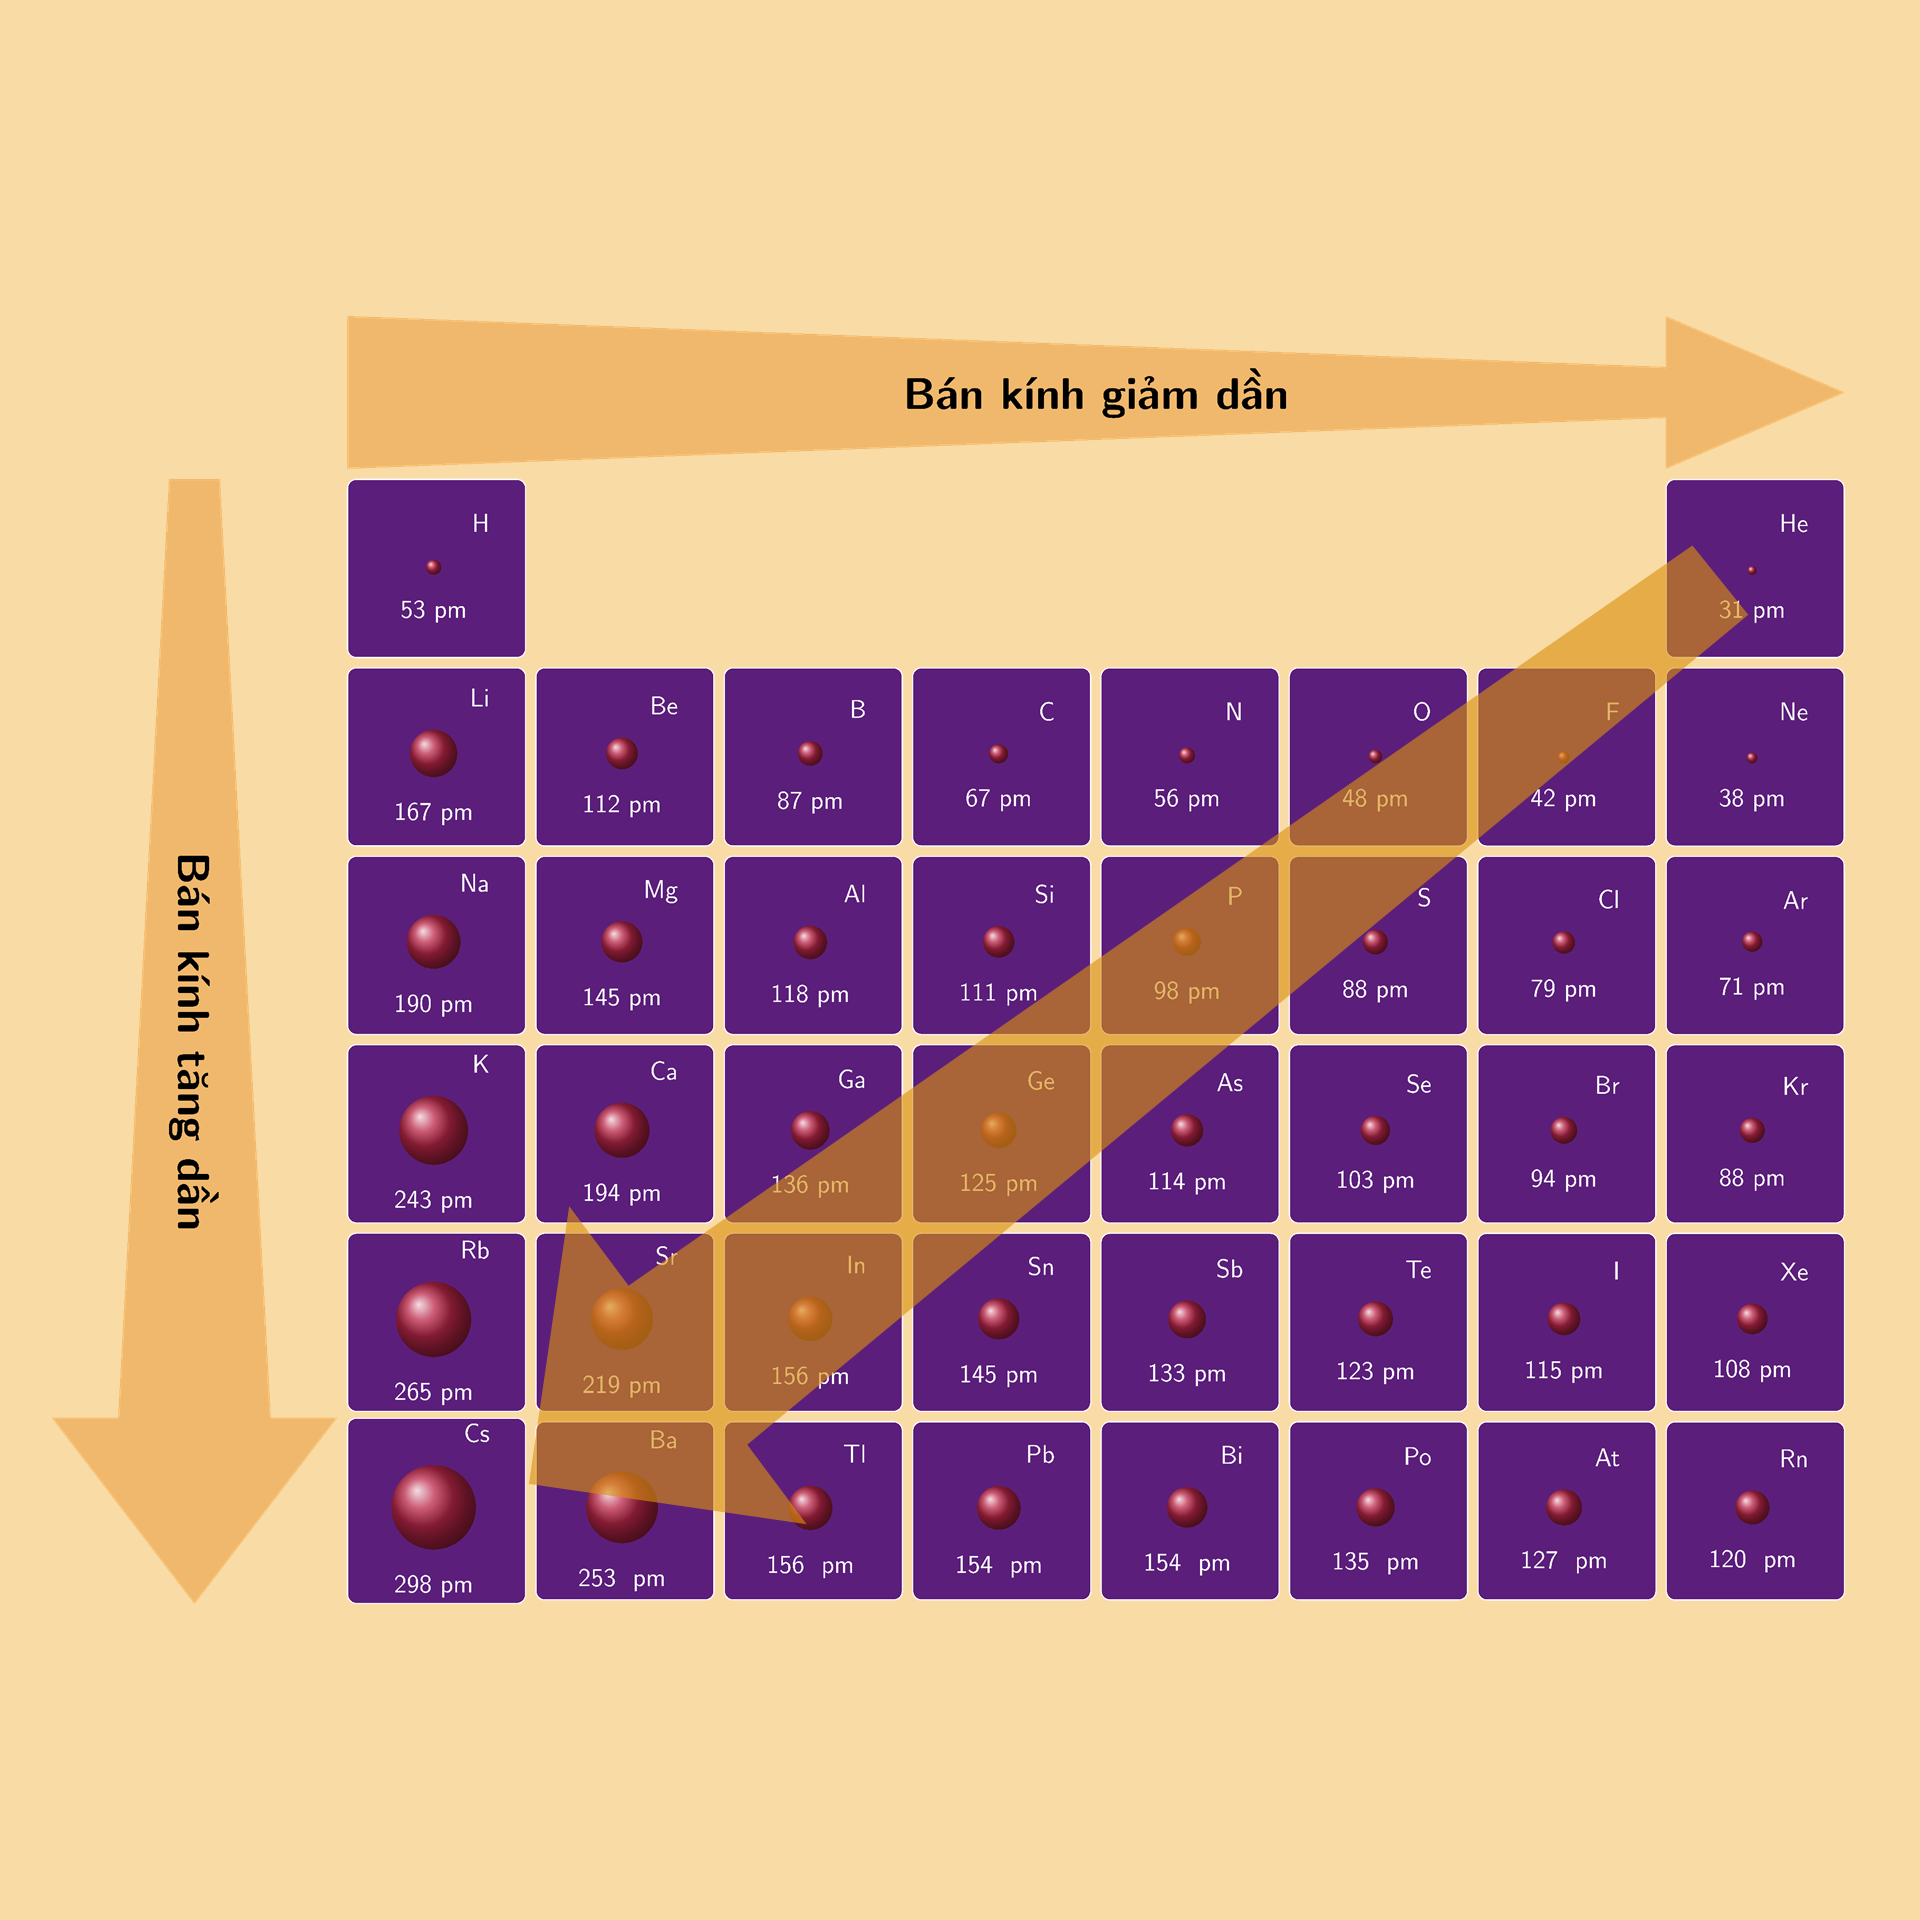
\includegraphics[width 	=8cm]{Images/anhminhoa/xuhuongbk.png}
	\end{center}
	\nhanmanh{Bài toán 2: So sánh bán kính ion}
	\GSND[\bfseries][\faBook][\maunhan]{Quy luât 1:}
%	\taodongke[\maunhan][1.12]{16}
	So với nguyên tử trung hòa
	\begin{enumerate}
		\item Khi một nguyên tử nhường e (cation) thì bán kính sẽ giảm đi
		\item Khi một nguyên tử nhận e (anion) thì bán kính nguyên tử sẽ tăng lên
	\end{enumerate}
	Do vây, đối với cùng nguyên tố thì:
	\begin{center}
		\boxct{Bán kính$_{cation}$ < bán kính $_{\text{nguyên tử}}$ < bán kính $_{anion}$}
	\end{center}
	\GSND[\bfseries][\faBook][\maunhan]{Quy luât 2:}
%	\taodongke[\maunhan][1.12]{18}
	Các ion có cùng số electron
	\begin{enumerate}
		\item Cation có điện tích càng lớn thì bán kính càng nhỏ
		\item Anion có điện tích càng lớn thì bán kính càng lớn
	\end{enumerate}
% \taodongke[\maunhan][1.12]{16}
\end{dangntd}
\newpage
\GSND[\bfseries][\faBookReader][\maudam]{Ví dụ mẫu:}
%%%==============VD_01===================%%%
\begin{vd}
	Hãy sắp xếp các nguyên tố $_{20}Ca$, $_{4}Be$, $_{12}Mg$ theo chiều tăng dần bán kính nguyên tử?
	\loigiai{
	Dựa vào  số hiệu nguyên tử các em viết cấu hình electron của các nguyên tử \Muiten{->} vị trí \Muiten{->} phác thảo lên bảng tuần hoàn  đưa ra quy luật biến đổi tính chất\\
	Ta có:\\
	$_{20}Ca: 1s^{2}2s^{2}2p^{6}3s^{2}3p^{6}4s^{2}$ \Muiten{->} Ca thuộc chu kì 4, nhóm IIA\\
	$_{4}Be: 1s^{2}2s^{2}$ \Muiten{->} Be thuộc chu kì 2, nhóm IIA\\
	$_{12}Mg: 1s^{2}2s^{2}2p^{6}3s^{2}$ \Muiten{->} Mg thuộc chu kì 3, nhóm IIA\\
	Ba nguyên tố Ca, Be, Mg thuộc cùng một nhóm nên chiều bán kính tăng dần là: Be < Mg < Ca
	}
\end{vd}
%%%==============VD_02===================%%%
\begin{vd}
	Hãy sắp xếp các nguyên tố $_{11}Na$, $_{17}Cl$, $_{15}P$, $_{13}Al$ theo chiều tăng dần bán kính nguyên tử?
	\sodongkevd[10]
\end{vd}
%%%==============VD_03===================%%%
\begin{vd}
	Hãy sắp xếp các nguyên tố $_{8}O$, $_{15}P$, $_{13}Al$, $_{20}Ca$, $_{19}K$ theo chiều tăng dần bán kính nguyên tử?
	\sodongkevd[10]
\end{vd}
%%%==============VD_04===================%%%
\begin{vd}
	Cho điện tích hạt nhân $O(Z=8), \mathrm{Na}(Z=11), \mathrm{Mg}(Z=12), \mathrm{Al}(Z=13)$ và các hạt vi mô: $O^{2-}, \mathrm{Al}^{3+}, \mathrm{Al}, \mathrm{Na}, \mathrm{Mg}^{2+}, \mathrm{Mg}$. Dãy nào sau đây được xếp đúng thứ tự bán kính hạt?
	\sodongkevd[15]
\end{vd}
%%%==============VD_05===================%%%
\begin{vd}
	Cho điện tích hạt nhân $O(Z=8), \mathrm{F}(Z=9), \mathrm{Mg}(Z=12), \mathrm{Al}(Z=13),\mathrm{S}(Z=16),\mathrm{Cl}(Z=17),\mathrm{K}(Z=19),\mathrm{Ca}(Z=20)$.Hãy sắp xếp dãy các ion sau: $\mathrm{S}^{2-},\mathrm{Cl}^{-},\mathrm{K}^{+},\mathrm{Ca}^{2+},\mathrm{Al}^{3+},\mathrm{Mg}^{2+},\mathrm{O}^{2-},\mathrm{F}^{-} $ theo chiều tăng dần của bán kính?
	\sodongkevd[15]
\end{vd}
%%%==========Nội dung file thứ 2===============%%%
\chapter{Liên kết hóa học}
\section{Quy tắc Octet}
\begin{mtbh}
	\begin{itemize}
		\item Trình bày được quy tắc octet với các nguyên tố nhóm $A$.
		\item Vận dụng được quy tắc octet trong quá trình hình thành liên kết hoá học ở các nguyên tố nhóm $A$.
	\end{itemize}
\end{mtbh}
\subsection{Kiến thức cần nhớ}
\begin{hoplythuyet}
	\GSND[\bfseries\sffamily][\faStar][\maunhan]{Liên kết hóa học:}
	Liên kết hóa học là sụ kết hợp giữa các nguyên tử tạo thành phân tử hay tinh thể bền vững hơn.
	\GSND[\bfseries\sffamily][\faStar][\maunhan]{Quy tắc octet:}
	Trong quá trình hình thành liên kết hóa học, nguyên tử của các nguyên tố nhóm A có xu hương tạo thành lớp vỏ ngoài cùng có 8 electron tương ứng với khí hiếm gần nhất (hoặc 2 electron với khí hiếm helium).
\end{hoplythuyet}
\begin{notegsnd}
	Không phải mọi trừờng hợp, nguyên tử của các nguyên tố khi tham gia liên kết đều tuân theo quy tắc octet. Người ta nhận thấy một số phân tủ không tuân theo quy tắc octet. Ví dụ: $\mathrm{NO}, \mathrm{BH}_3$, $S F_6, \ldots$
\end{notegsnd}

\columnratio{0.65}
\begin{paracol}{2}
	\begin{hoplythuyet}
		\GSND[\bfseries\sffamily][\faStar][\maunhan]{Liên kết hóa học:}
		Liên kết hóa học là sụ kết hợp giữa các nguyên tử tạo thành phân tử hay tinh thể bền vững hơn.
		\GSND[\bfseries\sffamily][\faStar][\maunhan]{Quy tắc octet:}
		Trong quá trình hình thành liên kết hóa học, nguyên tử của các nguyên tố nhóm A có xu hương tạo thành lớp vỏ ngoài cùng có 8 electron tương ứng với khí hiếm gần nhất (hoặc 2 electron với khí hiếm helium).
	\end{hoplythuyet}
	\switchcolumn 
	\begin{vdnote}
		Hai nguyên tử H liên kết với nhau tạo thành phân tử $H_2$ bền vững hơn nguyên tử H
	\end{vdnote}
	\begin{vdnote}
		Nguyên tử chlorine với cấu hình electron là $[\mathrm{Ne}] 3 \mathrm{~s}^2 3 \mathrm{p}^5$, có 7 electron ở lớp vỏ ngoài cùng.Khi hình thành liên kết hoá học chlorine nhận thêm 1 electron để đạt được lớp vỏ có 8 electron ở lớp ngoài cùng như của khí hiếm $\mathrm{Ar}$ (thay vì $\mathrm{Cl}$ phải nhường đi 7 electron để có lớp vỏ ngoài cùng là $2 \mathrm{~s}^2 2 \mathrm{p}^6$ - khó khăn hơn rất nhiều)
	\end{vdnote}
\end{paracol}

\newcommand{\ngoacvuongtron}[2][]{
	\begin{tikzpicture}[declare function={d=-4pt;},node distance=-d]
		\node (name) {#2};
		\node[anchor = base, above right =of name,shift={(-2pt,-5pt)}](plus) {$#1$};
		\draw[rounded corners=-d-1pt] (name.north west)--([xshift=d]name.north west)|-($(name.south west) +(0,0)$);
		\draw[rounded corners=-d-1pt] (name.north east)--([xshift=-d]name.north east)|-($(name.south east) +(0,0)$);
	\end{tikzpicture}
}
\newpage
\GSND[\bfseries\sffamily][\faStar][\maunhan]{Giải thích sự hình thành liên kết}
\columnratio{0.5}
\begin{paracol}{2}
	%%%================ Giải thích sự hình thành ion Cl ================%%%
	\begin{vdnote}
		Nguyên tử chlorine với cấu hình electron là $[Ne]3s^23p^5$, có 7 electron ở lớp ngoài cùng. Vậy có xu hướng nhận thêm 1 electron để đạt cấu hình bền vững giống khí hiếm Ar (hình \ref{ion_Cl})
	\end{vdnote}
	\begin{center}
		\begin{tikzpicture}[declare function ={k=5cm;},node distance=1.5cm]
			\node at (0:0) (Cl) {
				\begin{tikzpicture}[declare function={r=.5 cm;}]
					\tikzstyle{mystyle} = [draw=red,inner sep = 0pt,anchor=center, baseline]
					\path (0:0) coordinate (O);
					\fill[ball color=red!50](O) circle (r -.25 cm);
					\node[font=\tiny] at (O) {\textbf{+17}};
					\draw[mystyle] (O) circle (r+0.25cm);
					\foreach \g in {0,45,90,135,180,225,270,315}{\fill[ball color =\mauphu!50] (\g:{r+0.25cm}) circle (1pt);}
					\draw[mystyle] (O) circle (r+0.25*2cm);
					\foreach \g in {45,90,135,180,225,270,315}{\fill[ball color =\mauphu!50] (\g:{r+0.25*2cm}) circle (1pt);}
					\draw[mystyle] (O) circle (r);
					\foreach \g in {90,-90}{\fill[ball color =\mauphu!50] (\g:r) circle (1pt);}
				\end{tikzpicture}
			};
			\node[yshift=7pt] at (0:k)(ion-Cl) {
				\ngoacvuongtron[-]{\begin{tikzpicture}[declare function={r=.5 cm;},scale=1.2]
						\tikzstyle{mystyle} = [text centered, draw=red,inner sep = 0pt]
						\path (0:0) coordinate (O);
						\fill[ball color=red!50](O) circle (r -.25 cm);
						\node[font=\tiny] at (O) {\textbf{+17}};
						\draw[mystyle] (O) circle (r+0.25cm);
						\foreach \g in {0,45,90,135,180,225,270,315}{\fill[ball color =\mauphu!50] (\g:{r+0.25cm}) circle (1pt);}
						\draw[mystyle] (O) circle (r+0.25*2cm);
						\foreach \g in {0,45,90,135,180,225,270,315}{\fill[ball color =\mauphu!50] (\g:{r+0.25*2cm}) circle (1pt);}
						\draw[mystyle] (O) circle (r);
						\foreach \g in {90,-90}{\fill[ball color =\mauphu!50] (\g:r) circle (1pt);}
				\end{tikzpicture}}
			};
			\draw[-latex,line width=1pt] (Cl.east)--([yshift=-7pt]ion-Cl.west)node[midway,pos =0.5,above,font=\sf\small,yshift=-2pt]{nhận}node[midway,pos =0.5,below,font=\sf\small,yshift=2pt]{1 electron};
			\node [below of= Cl,font=\bfseries\small] {Cl};
			\node [below of= ion-Cl,font=\bfseries\small,shift={(-6pt,-9pt)}] {\text{Cl$^{-}$}};
		\end{tikzpicture}
		\captionof{figure}{Sơ đồ nguyên tử Cl nhận thêm 1 eclectron vào lớp ngoài cùng \label{ion_Cl}}
	\end{center}
	\switchcolumn
	%%%================Giải thích sự hình thành ion Na================%%%
	\begin{vdnote}
		Nguyên tử Sodium với cấu hình $[Ne]3s^1$, có 1 electron ở lớp ngoài cùng .Vậy xu hướng khi hình thành liên kết là nhường đi 1 electron để đạt được cấu hình electron giống khí hiếm Ne.(hình \ref{ion_Na})
	\end{vdnote}
	\begin{center}
		\begin{tikzpicture}[declare function ={k=5cm;},node distance=1.5cm]
			\node at (0:0) (Na) {
				\begin{tikzpicture}[declare function={r=.5 cm;}]
					\tikzstyle{mystyle} = [draw=red,inner sep = 0pt,anchor=center, baseline]
					\path (0:0) coordinate (O);
					\fill[ball color=red!50](O) circle (r -.25 cm);
					\node[font=\tiny] at (O) {\textbf{+11}};
					\draw[mystyle] (O) circle (r+0.25cm);
					\foreach \g in {0,45,90,135,180,225,270,315}{\fill[ball color =\mauphu!50] (\g:{r+0.25cm}) circle (1pt);}
					\draw[mystyle] (O) circle (r+0.25*2cm);
					\foreach \g in {0}{\fill[ball color =\mauphu!50] (\g:{r+0.25*2cm}) circle (1pt);}
					\draw[mystyle] (O) circle (r);
					\foreach \g in {90,-90}{\fill[ball color =\mauphu!50] (\g:r) circle (1pt);}
				\end{tikzpicture}
			};
			\node[yshift=7pt] at (0:k)(ion-Na) {
				\ngoacvuongtron[+]{\begin{tikzpicture}[declare function={r=.5 cm;},scale=1.2]
						\tikzstyle{mystyle} = [text centered, draw=red,inner sep = 0pt]
						\path (0:0) coordinate (O);
						\fill[ball color=red!50](O) circle (r -.25 cm);
						\node[font=\tiny] at (O) {\textbf{+11}};
						\draw[mystyle] (O) circle (r+0.25cm);
						\foreach \g in {0,45,90,135,180,225,270,315}{\fill[ball color =\mauphu!50] (\g:{r+0.25cm}) circle (1pt);}
						\draw[mystyle] (O) circle (r);
						\foreach \g in {90,-90}{\fill[ball color =\mauphu!50] (\g:r) circle (1pt);}
				\end{tikzpicture}}
			};
			\draw[-latex,line width=1pt] (Na.east)--([yshift=-7pt]ion-Na.west)node[midway,pos =0.5,above,font=\sf\small,yshift=-2pt]{nhường}node[midway,pos =0.5,below,font=\sf\small,yshift=2pt]{1 electron};
			\node [below of= Na,font=\bfseries\small] {Na};
			\node [below of= ion-Na,font=\bfseries\small,shift={(-6pt,-9pt)}] {\text{Na$^{+}$}};
		\end{tikzpicture}
		\captionof{figure}{Sơ đồ nguyên tử Na nhường đi 1 eclectron  \label{ion_Na}}
	\end{center}
\end{paracol}

\columnratio{0.5}
\begin{paracol}{2}
%%%================Giải thích sự hình thành phân tử H2================%%%		
	\begin{vdnote}
		Phân tử $\mathrm {H_2}$ được hình thành từ hai nguyên tử H bởi sự góp chung electron (hình \ref{hthidro})
	\end{vdnote}
	\begin{center}
		\tikzstyle{mystyle} = [draw=\mauphu!90!black,inner sep = 0pt,anchor=center, baseline,fill=\mauphu!90,opacity=.5,line width=.8pt]
		\begin{tikzpicture}[declare function ={k=1.8cm;},node distance=.5pt and .5pt]
			\node at (0:0) (H1) {
				\begin{tikzpicture}[declare function={r=.5 cm;}]
					\path (0:0) coordinate (O);
					\fill[ball color=\mauphu!90](O) circle (r -.25 cm);
					\node[font=\tiny] at (O) {\textbf{+1}};
					\filldraw[mystyle] (O) circle (r+0.25cm);
					\foreach \g in {25}{\fill[ball color =\mauphu!90] (\g:{r+0.25cm}) circle (1.5pt);}
				\end{tikzpicture}
			};
			\node [below=of H1]{\bf H};
			\node at (0:k)(H2) {
					\begin{tikzpicture}[declare function={r=.5 cm;}]
					\path (0:0) coordinate (O);
					\fill[ball color=\mauphu!90](O) circle (r -.25 cm);
					\node[font=\tiny] at (O) {\textbf{+1}};
					\filldraw[mystyle] (O) circle (r+0.25cm);
					\foreach \g in {205}{\fill[ball color =\mauphu!90] (\g:{r+0.25cm}) circle (1.5pt);}
				\end{tikzpicture}
			};
			\node [below=of H2]{\bf H};
			\node at (0:{3*k})(H3){
			\begin{tikzpicture}[declare function={r=.5 cm;}]
				\path (0:0) coordinate (O);
				\fill[ball color=\mauphu!90](O) circle (r -.25 cm);
				\node[font=\tiny] at (O) {\textbf{+1}};
				\filldraw[mystyle] (O) circle (r+0.25cm);
				\foreach \g in {-10}{\fill[ball color =\mauphu!90] (\g:{r+0.12cm}) circle (1.5pt);}
			\end{tikzpicture}
			};
			\node at (0:{3.68*k})(H4){
				\begin{tikzpicture}[declare function={r=.5 cm;}]
					\path (0:0) coordinate (O);
					\fill[ball color=\mauphu!90](O) circle (r -.25 cm);
					\node[font=\tiny] at (O) {\textbf{+1}};
					\filldraw[mystyle] (O) circle (r+0.25cm);
					\foreach \g in {170}{\fill[ball color =\mauphu!90] (\g:{r+0.12cm}) circle (1.5pt);}
				\end{tikzpicture}
			};
			\filldraw[-{Latex[length=5mm]},line width=6pt,draw=\mauphu,] (H2.east)--(H3.west) ;
			\node [below=of H3,xshift={.34*k}]{ $\mathbf {H_2}$};
		\end{tikzpicture}
		\captionof{figure}{Sự góp chung electron trong phân tử hiđro \label{hthidro}}
	\end{center}
		\switchcolumn
	%%%================Giải thích sự hình thành phân tử N2================%%%
	\begin{vdnote}
		Phân tử $\mathrm {N_2}$ được hình thành từ hai nguyên tử N bởi sự góp chung của 3 cặp electron (hình \ref{htnito})
	\end{vdnote}
	\begin{center}
		\tikzstyle{mystyle} = [draw=\mycolor!90!black,inner sep = 0pt,anchor=center, baseline,fill=\mycolor!90,opacity=.3,line width=.8pt]
		\begin{tikzpicture}[declare function ={k=2.5cm;R=1.2cm;},node distance=.5pt and .5pt]
			\node at (0:0) (N1) {
				\begin{tikzpicture}[declare function={r=.5 cm;}]
					\path (0:0) coordinate (O);
					\fill[ball color=\mycolor!90](O) circle (r -.25 cm);
					\node[font=\tiny] at (O) {\textbf{+7}};
					\filldraw[mystyle] (O) circle (r);
					\foreach \g in {90,-90}{\fill[ball color =\mycolor!70] (\g:{r}) circle (1.5pt);}
					\filldraw[mystyle] (O) circle (r+0.25cm);
					\foreach \g in {170,-170,45,-45,0}{\fill[ball color =\mycolor!90] (\g:{r+0.25cm}) circle (1.5pt);}
				\end{tikzpicture}
			};
%	
			\node at (0:.5*k) (plus){\large +};
			\node at (0:k) (N2) {
				\begin{tikzpicture}[declare function={r=.5 cm;}]
					\path (0:0) coordinate (O);
					\fill[ball color=\mycolor!90](O) circle (r -.25 cm);
					\node[font=\tiny] at (O) {\textbf{+7}};
				\begin{scope}[transform canvas={xscale=-1}]
					\filldraw[mystyle] (O) circle (r);
					\foreach \g in {90,-90}{\fill[ball color =\mycolor!70] (\g:{r}) circle (1.5pt);}
					\filldraw[mystyle] (O) circle (r+0.25cm);
					\foreach \g in {170,-170,45,-45,0}{\fill[ball color =\mycolor!90] (\g:{r+0.25cm}) circle (1.5pt);}
				\end{scope}
				\end{tikzpicture}
			};
			
			\node at (0:{2.4*k}) (N3) {
				\begin{tikzpicture}[declare function={r=.5 cm;}]
					\path (0:0) coordinate (O);
					\fill[ball color=\mycolor!90](O) circle (r -.25 cm);
					\node[font=\tiny] at (O) {\textbf{+7}};
					\begin{scope}[transform canvas={xscale=1}]
						\filldraw[mystyle] (O) circle (r);
						\foreach \g in {90,-90}{\fill[ball color =\mycolor!70] (\g:{r}) circle (1.5pt);}
						\filldraw[mystyle] (O) circle (r+0.25cm);
						\foreach \g in {170,-170}{\fill[ball color =\mycolor!90] (\g:{r+0.25cm}) circle (1.5pt);}
					\end{scope}
				\end{tikzpicture}
			};
				\node at (0:{2.90*k}) (N4) {
				\begin{tikzpicture}[declare function={r=.5 cm;}]
					\path (0:0) coordinate (O);
					\fill[ball color=\mycolor!90](O) circle (r -.25 cm);
					\node[font=\tiny] at (O) {\textbf{+7}};
					\begin{scope}[transform canvas={xscale=-1}]
						\filldraw[mystyle] (O) circle (r);
						\foreach \g in {90,-90}{\fill[ball color =\mycolor!70] (\g:{r}) circle (1.5pt);}
						\filldraw[mystyle] (O) circle (r+0.25cm);
						\foreach \g in {170,-170}{\fill[ball color =\mycolor!90] (\g:{r+0.25cm}) circle (1.5pt);}
					\end{scope}
				\end{tikzpicture}
			};
			\node at (0:{2.4*k+.56cm}) {\tikz{\fill[ball color =\mycolor!90]circle (1.45pt);}};
			\node at (0:{2.4*k+.7cm}) {\tikz{\fill[ball color =\mycolor!90]circle (1.45pt);}};
			\node at ([yshift=4pt]0:{2.4*k+.57cm}) {\tikz{\fill[ball color =\mycolor!90]circle (1.45pt);}};
			\node at ([yshift=4pt]0:{2.4*k+.68cm}) {\tikz{\fill[ball color =\mycolor!90]circle (1.45pt);}};
			\node at ([yshift=-4pt]0:{2.4*k+.57cm}) {\tikz{\fill[ball color =\mycolor!90]circle (1.45pt);}};
			\node at ([yshift=-4pt]0:{2.4*k+.68cm}) {\tikz{\fill[ball color =\mycolor!90]circle (1.45pt);}};
			\filldraw[-{Latex[length=5mm]},line width=6pt,draw=\mycolor,] ([xshift=.5cm]N2.east)--([xshift=-.5cm]N3.west) ;
			\node at ([yshift=-4pt]0:{2.4*k+.68cm}) {\tikz{\fill[ball color =\mycolor!90]circle (1.45pt);}};
			\node at ([yshift=-R]0:0) {\large N};
			\node at ([yshift=-R]0:{k}) {\large N};
			\node at ([yshift=-R]0:{2.65*k}) {\large $\mathbf{N_2}$};
		\end{tikzpicture}
		\captionof{figure}{Sự góp chung electron trong phân tử nitơ \label{htnito}}
	\end{center}
\end{paracol}
\subsection{Bài tập}
%%%===============Câu_01=======================%%%		
\begin{ex}[][Quy tắc octet]
	Biết phân tử magnesium được hình thành từ các ion $Mg^{2+}$ và ion $O^{2-}$.Vận dụng quy tắc octet, trình bày sự hình thành các ion trên từ những nguyên tử tương ứng.
	\huongdan{
	\begin{itemize}
		\item Mg (Z=12):$1s^22s^22p^63s^2$ (có 2 electron ở lớp ngoài cùng) $\Rightarrow$ $Mg \longrightarrow$ $Mg^{2+} + 2e$
		\item O (Z=8):$1s^22s^2p^4$ (có 6 electron ở lớp ngoài cùng) $\Rightarrow$ $O + 2e \longrightarrow$ $O^{2-} $
	\end{itemize}
	
	}
\end{ex}
%%%===============Câu_02=======================%%%		
\begin{ex}[][Quy tắc octet]
	Cho các nguyên tử của các nguyên tố sau:Na(Z=11), Cl(Z=17), Ne(Z=10), Ar(Z=18).Những nguyên tử nào trong các nguyên tử trên có lớp electron bền vững.
	\huongdan{
		\begin{multicols}{2}
			\begin{itemize}
			\item Na (Z=11):$1s^22s^22p^63s^1$ 
			\item Cl (Z=17):$ 1s^22s^22p^63s^23p^5$
			\item Ne (Z=10):$ 1s^22s^22p^6$
			\item Ar (Z=18):$ 1s^22s^22p^63s^23p^6$
		\end{itemize}
		\end{multicols}
	}
\end{ex}















%\newpage
%\setchemfig{%
%	atom sep= 2em,
%	bond offset=2pt,
%	compound sep=5em
%}

%\schemestart
%\chemname{\chemfig{
%H-@{N}\charge{0:2pt=\:}{N}(-[6]H)-[2]H
%}}{\scriptsize\quad\quad Ammonia\vphantom{aa}}
%\+
%\chemfig{
%@{H}\charge{45:3pt=$\scriptstyle+$}{H}
%}
%\arrow(.mid east--.mid west)[,.7,-latex]
%\chemname{\ngoacvuongtron{\chemfig{
%			H-N(-[2]H)(-[6]H)-[,,,,-stealth]H
%}}}{\scriptsize Ammonium\quad}
%\schemestop
%
%\chemmove[shorten <=4pt,shorten >=4pt,-latex] {
%\draw ([shift={(-25:3.5pt)}]N.25).. controls +(80:8mm) and +(100:8mm)..([shift={(29:3.5pt)}]H.65)
%;}
%%%%=============Tinh thể NaCl===================%%%
%\begin{tikzpicture}[node distance=0pt]
%	% Định dạng cho cột của bảng
%	\tikzset{%
%		%% Định dạng ô
%		mynode/.style={%
%			circle,
%			ultra thin,
%			minimum height=0.65cm,
%			minimum width=0.65cm,
%			align=center
%		},
%		mymatrix/.style={%
%			matrix of nodes,
%			ampersand replacement=\&,
%			inner sep =5pt,
%			nodes in empty cells,
%			fill =\mycolor!15,
%			row sep=-3-\pgflinewidth,
%			column sep=-3-\pgflinewidth,
%			nodes={mynode}
%		}
%	}
%	\matrix(Bang)[mymatrix]{%
%	\&\&\&\&\&\\
%	\&\&\&\&\&\\
%	\&\&\&\&\&\\
%	\&\&\&\&\&\\
%	\&\&\&\&\&\\
%	};
%\foreach \x in {1,3,5}{
%	\foreach \y in {1,3,5}{
%	\fill [ball color=\maunhan!70 ] (Bang-\x-\y) circle (0.3cm) node[font=\tiny\sffamily\bfseries\color{white}](Na) {Na} ;
%	\node [font=\fontsize{5pt}{3pt}\selectfont\sffamily\bfseries\color{white}] at ([shift={(60:4.8pt)}]Bang-\x-\y) {+};
%	}
%}
%\foreach \x in {2,4}{
%	\foreach \y in {2,4,6}{
%		\fill [ball color=\maunhan!70 ] (Bang-\x-\y) circle (0.3cm);
%	}
%}
%\foreach \x in {1,3,5}{
%	\foreach \y in {2,4,6}{
%		\fill [ball color=\maudam!70 ] (Bang-\x-\y) circle (0.2cm);
%	}
%}
%\foreach \x in {2,4}{
%	\foreach \y in {1,3,5}{
%		\fill [ball color=\maudam!70 ] (Bang-\x-\y) circle (0.2cm);
%	}
%}
%\end{tikzpicture}
%%%==========Nội dung file thứ 3===============%%%
\newenvironment{cacbuoc}{\begin{enumerate}[label= \color{\maunhan}\bfseries\fontfamily{qag}\selectfont{\faAdjust\;Bước \arabic*:},itemsep=0pt,wide=0cm,leftmargin=0.5cm,topsep=0pt]
	}{\end{enumerate}}
\newtcolorbox{body}{%
	enhanced,
	before skip=1cm,
	breakable,
	colback=\mycolor!20,
	enhanced jigsaw,opacityback=0,opacitybacktitle=0,
	opacityback=0,
	colframe=\mycolor
}
\renewcommand{\thesubsubsection}{\Roman{subsubsection}}
\titlespacing*{\subsection}{3pt}{0pt}{-5pt}
\titlespacing*{\subsubsection}{3pt}{5pt}{-5pt}
\titlespacing*{\paragraph}{0cm}{0cm}{-5pt}
\setcounter{chapter}{3}
\chapter{Phản ứng Oxi hóa - khử}
\section{Số Oxi hóa - Cân bằng phản ứng oxi hóa khử}
\subsection{Kiến thức cần nhớ}
\begin{body}
	\subsubsection{Số oxi hóa}
	\begin{dn}
		\indam{Số oxi hóa} của một nguyên tử một nguyên tố trong hơp chất là \indam{điện tích} của nguyên tử nguyên tố đó với giả định đây là hợp chất ion.
	\end{dn}
	\subsubsection{Cách xác định số oxi - hóa}
	\begin{enumerate}
		\item \indam{Quy tắc 1:}
		Trong đơn chất, số oxi hóa của các nguyên tố bằng 0.\\
		VD: $\overset{0}{\mathrm{H}_{2}}$, $\overset{0}{\mathrm{Na}}$, $\overset{0}{\mathrm{O}_{3}}$, $\ldots$
		\item \indam{Quy tắc 2:}
		Trong một phân tử,tổng số oxi hóa  của các nguyên tố nhân với số nguyên tử của từng nguyên tố bằng 0\\
		\item \indam{Quy tắc 3:} 
		\begin{itemize}
			\item Trong các ion \indam{đơn nguyên tử}, số oxi hóa của các nguyên tố bằng điệnu tích của ion đó\\
			\item Trong ion \indam{đa nguyên tử}, tổng số oxi hóa các nguyên tố nhân với số nguyên tử của từng nguyên tố bằng điện tích của ion
		\end{itemize}
		\item \indam{Quy tắc 4:} \\
		\begin{itemize}
			\item Trong đa số các hợp chất, số oxi hóa của hydrogen bằng +1 , trừ hydride kim loại ($NaH$, $CaH_2$)\\
			\item Số oxi hóa của oxygen bằng $-\mathrm{2}$, trừ trường hợp $\overset{+1}{\mathrm{O}_{}}\overset{\vphantom{-1}}{\mathrm{F}_{2}}$ và peoxit $\left(\overset{\vphantom{+1}}{\mathrm{Na}_{2}}\overset{-1}{\mathrm{O}_{2}}\right)$, superoxide $\left(\overset{\vphantom{+1}}{\mathrm{K}_{}}\overset{-\tfrac{1}{2}}{\mathrm{O}_{2}}, \ldots\right)$.\\
			\item Các nguyên tố nhóm IA, IIA luôn có số oxi hóa $+1,+2$, số oxi hóa của $\mathrm{Al}$ là +3 . Số oxi hóa của nguyên tử nguyên tố fluorine trong các hợp chất bằng -1
		\end{itemize}
	\end{enumerate}
	\subsubsection{Phản ứng Oxi hóa - khử}
	\paragraph{Sự oxi hóa-sự khử}
	\begin{mylt}
		\begin{enumerate}[label = \indam{\alph*)}]
			\item \indam{Sự oxi hóa} là sự nhường electron, là sự tăng số oxi hóa.\\
			\indam{Ví dụ:} $\overset{0}{Mg} \rightarrow Mg^{2+} + 2e$
			\item \indam{Sự khử} là sự thu electron, là sự giảm electron.\\
			\indam{Ví dụ:} $Cu^{2+} +2e \rightarrow Cu $
		\end{enumerate}
	\end{mylt}
	\paragraph{Chất oxi hóa - chất khử}
	\begin{mylt}
		\begin{enumerate}[label = \indam{\alph*)}]
			\item \indam{Chất oxi hóa} là chất thu electron.là chất chứa nguyên tố có số oxi hóa giảm sau phản ứng.\\
			\indam{Chất oxihóa} còn gọi là chất \indam{bị khử}.
			\item \indam{Chất khử} là chất nhường electron, là chất có số oxi hóa tăng sau phản ứng\\
			\indam{Chất khử} còn gọi là chất \indam{bị oxi hóa}.
		\end{enumerate}
	\end{mylt}
	\begin{vdnote}
		$ \overset{0}{Mg} + \overset{+2}{Cu}SO_{4} \rightarrow\overset{+2}{Mg}SO_{4}  + \overset{0}{Cu}$.\\
		$Cu^{2+}$ nhận electron, là chất oxi hóa ( số oxi hóa giảm từ +2 về 0).
		$Mg$ nhường electron, là chất khử (số oxi hóa tăng từ 0 lên +2)
	\end{vdnote}
	\begin{vdnote}
		$\overset{+3}{Fe_2}\overset{\vphantom{+3}}{O_3} + 3\overset{+2}{C}O$ $\longrightarrow$ $ 2 \overset{0}{Fe} + 3\overset{+4}{C}O_2$
	\end{vdnote}
	\paragraph{Phản ứng Oxi hóa - khử }
	\begin{mylt}
		\indam{Phản ứng oxi - hóa khử } là phản ứng hóa học trong đó có sự chuyển electron giữa các chất phản ứng.\\
		Nếu dựa vào sự thay đổi số oxi hóa thì phản ứng oxi hóa-khử là phản ứng hóa học trong đó có sự  thay đổi số oxi hóa của một số nguyên tố.\\
		
		\begin{vdnote}
			\[\begin{tikzpicture}
				\tikzstyle{mynode} =[
				font=\normalsize,
				line width =.8pt,
				anchor=center,
				align =center,
				]
				%%%==================%%%
				\tikzstyle{mymatrix} = [
				matrix of nodes,
				nodes in empty cells,
				nodes={mynode},
				column sep=-\pgflinewidth,
				row sep = -\pgflinewidth,
				minimum width = .5cm,
				minimum height = .6cm,
				column 4/.style={
					minimum width = .7cm,
				},
				]
				%%%=======================================================%%%
				\matrix(m) [mymatrix]{
					Mg & + & $CuSO_4$ & [-.7cm]\muiten[][][0.7]{->}& $MgSO_4$ & + & Cu\\
				};
				\node(0)[yshift=4pt,\maunhan] at (m-1-1.north){0};
				\node(2)[xshift =-8pt,yshift=4pt,\maunhan] at (m-1-3.north){+2};
				\node[xshift =-8pt,yshift=4pt,\maunhan] at (m-1-5.north){+2};
				\node[yshift=4pt,\maunhan] at (m-1-7.north){0};
				\draw[->,>=stealth,violet,ultra thick](0.90)--++(90:.5cm)-|(2.90) ;
				\path ($(0.90)+(90:.5cm)$)-- ($(2.90)+(90:.5cm)$) node [pos=.5,above,violet]{- 2 e};
			\end{tikzpicture}\]
			Trong phản ứng trên $Mg$ nhường đi 2 electron cho ion $Cu^{+2}$ trở thành ion $Mg^{+2}$ và ion $Cu^{+2}$ nhận  2 electron từ nguyên tử $Mg$ trở thành nguyên tử Cu.
		\end{vdnote}
		%%%===============Môi Trường Matrix=================%%%
	\end{mylt}
	\subsubsection{Cân bằng phản ứng oxi hóa-khử}
	\begin{mylt}
		\GSND[\bfseries\sffamily][\faStar]{Phương pháp thăng bằng electron:}\\
		Phương pháp này dựa trên nguyên tắc:
		\boxct[\mauphu][3pt][\bfseries\sffamily\color{violet}]{Tổng số electron chất khử nhường  = tổng số electron mà chất oxi hóa nhận}
		\indam{\faBook\ Các bước cân bằng:}\vspace{.5cm}
		\begin{vdnote}
			Lập phương trình phản ứng Oxi hóa - khử sau: 
			\[\puhh[$t^{\circ}$]{$Cu$\+ $HNO_3$}{->}{$Cu({NO_3})_2$ \+ $NO\uparrow$ \+ $H_2O$}\]
		\end{vdnote}
		\indam{\itshape Hướng dẫn giải:}
		\begin{cacbuoc}
			\item Xác định số oxi hóa của nguyên tử cóa sự thay đổi số oxi hóa, xác định chất khử, chất oxi hóa
			\[\begin{tikzpicture}
				\tikzstyle{mynode} =[
				font=\normalsize,
				line width =.8pt,
				anchor=center,
				align =center,
				]
				%%%==================%%%
				\tikzstyle{mymatrix} = [
				matrix of nodes,
				nodes in empty cells,
				nodes={mynode},
				column sep=-\pgflinewidth,
				row sep = -\pgflinewidth,
				minimum width = .5cm,
				minimum height = .6cm,
				column 4/.style={
					minimum width = .7cm,
				},
				]
				%%%=======================================================%%%
				\matrix(m) [mymatrix]{
					$Cu$ & + & $HNO_3$ & [-.7cm]\muiten[][][0.7]{->}& $Cu({NO_3})_{2}$ & + & $NO\uparrow$ & + & $H_2O$ \\
				};
				\node(0)[yshift=4pt,\maunhan] at (m-1-1.north){0};
				\node(chatkhu)[yshift=-4pt,\maunhan,font=\footnotesize] at (m-1-1.south){(Chất khử)};
				\node(2)[xshift =-2pt,yshift=4pt,\maunhan] at (m-1-3.north){+5};
				\node(chatoxh)[yshift=-4pt,\maunhan,font=\footnotesize] at (m-1-3.south){(Chất oxi hóa)};
				\node[xshift =-18pt,yshift=4pt,\maunhan] at (m-1-5.north){+3};
				\node[xshift =-8pt,yshift=4pt,\maunhan] at (m-1-7.north){+2};
			\end{tikzpicture}\]
			\item Viết quá trình oxi hóa và quá trình khử
			\[\begin{tikzpicture}
				\tikzstyle{mynode} =[
				font=\normalsize,
				line width =.8pt,
				anchor=center,
				align =center,
				minimum width = 0.4cm,
				minimum height = 1.0cm,
				]
				%%%==================%%%
				\tikzstyle{mymatrix} = [
				matrix of nodes,
				nodes in empty cells,
				nodes={mynode},
				column sep=-\pgflinewidth,
				row sep = 2pt-\pgflinewidth,
				column 1/.style={
					minimum width = 4cm,
					anchor =east,
					align =center,
				},
				]
				%%%=======================================================%%%
				\matrix(m) [mymatrix]{
					\text{Quá trình oxi hóa :} & Cu & [-.5cm]\muiten[][][0.4]{->}& Cu & + & 2e\\
					\text{Quá trình khử :} & N & + & [-.5cm]3e & [-.5cm]\muiten[][][0.4]{->} & NO\\
				};
				\node(0)[yshift=-2pt,\maunhan] at (m-1-2.north){0};
				\node(3)[yshift=-2pt,\maunhan] at (m-1-4.north){+2};
				\node(5)[yshift=-2pt,\maunhan] at (m-2-2.north){+5};
				\node(2)[xshift=-2pt,yshift=-2pt,\maunhan] at (m-2-6.north){+2};
			\end{tikzpicture}\]
			\item Nhân hệ số thích hợp  vào các quá trình  sao cho tổng  số electron chất khử nhường  bằng tổng số electron chất oxi hóa nhận.
			\[\begin{tikzpicture}
				\tikzstyle{mynode} =[
				font=\normalsize,
				line width =.8pt,
				anchor=center,
				align =center,
				minimum width = 0.4cm,
				minimum height = 1.0cm,
				]
				%%%==================%%%
				\tikzstyle{mymatrix} = [
				matrix of nodes,
				nodes in empty cells,
				nodes={mynode},
				column sep=3pt-\pgflinewidth,
				row sep = 2pt-\pgflinewidth,
				column 1/.style={
					minimum width = 4cm,
					anchor =east,
					align =center,
				},
				]
				%%%=======================================================%%%
				\matrix(m) [mymatrix]{
					3 x & Cu & [-.5cm]\muiten[][][0.4]{->}& Cu & + & 2e\\
					2 x & N & + & [-.5cm]3e & [-.5cm]\muiten[][][0.4]{->} & NO\\
				};
				\node(0)[yshift=-2pt,\maunhan] at (m-1-2.north){0};
				\node(3)[yshift=-2pt,\maunhan] at (m-1-4.north){+2};
				\node(5)[yshift=-2pt,\maunhan] at (m-2-2.north){+5};
				\node(2)[xshift=-2pt,yshift=-2pt,\maunhan] at (m-2-6.north){+2};
				\draw[\maunhan,line width=1pt] (m-1-1.north east)--(m-2-1.south east);
			\end{tikzpicture}\]
			\item Đặt các hệ số vào sơ đồ phản ứng. Can bằng số lượng  nguyên tử của các nguyên tố còn lại.
			\[\puhh[$t^{\circ}$]{$3Cu$ \+ ${8HNO_3}_{\text{loãng}}$}{->}{$3Cu({NO_3})_{2}$ \+ $2NO$ \+ $4H_2O$}\]
		\end{cacbuoc}
	\end{mylt}
\end{body}
\newpage
\subsection{Các dạng bài tập}
\begin{dangNTD}{Câu hỏi lý thuyết về phản ứng oxi hóa khử}
\end{dangNTD}
\begin{vdm}
\end{vdm}

\hienthiloigiaivd
%%%=========vd_1=========%%%
\begin{vd}[1][Nhận biết các quá trình vai trò của các chất]Một nguyên tử nhôm (Al) chuyển thành ion $Al^{3+}$ thực hiện :
	\choice
	{%
		nhận thêm 3 electron (quá trình oxi hóa)
	}{%
		nhường đi 3 electron (quá trình khử)
	}{%
		nhận thêm 3 electron (quá trình khử)
	}{%
		\True nhường đi 3 electron (quá trình oxi hóa)
	}
	\loigiai{Quá trình oxi hóa  một chất là làm cho nguyên tử trong chất đó nhường electron hay làm tăng số oxi hóa của nguyên tử trong chất đó.\\
		Quá trình khử  một chất là làm cho nguyên tử trong chất đó nhận electron hay làm giảm số oxi hóa của nguyên tử trong chất đó.\\
		Ta thấy số oxi hóa của nhôm tăng (quá trình oxi hóa) \\
		$\begin{matrix}
			\overset{0}{Al}& \muiten[][][.4]{->} &\overset{+3}{Al} & + & 3e
		\end{matrix}$
	}
\end{vd}
%%%=========vd_2=========%%%
\begin{vd}[2][Nhận biết các quá trình vai trò của các chất]Trong phản ứng : \puhh{$Cl_2$\+ $2KBr$}{->}{$Br_2$\+ 2KCl}, $Cl_2$ đóng vai trò 
	\choice{%
		\True là chất oxi hóa
	}{%
		là chất khử
	}{%
		không bị oxi hóa, không bị khử
	}{%
		vừa bị oxi hóa, vừa bị khử.
	}
	\loigiai{Chất oxi hóa là chất nhận electron hay là chất có số oxi hóa giảm sau phản ứng.\\
		Chất khử là chất nhường electron hay là chất có số oxi hóa tăng sau phản ứng.\\
		Ta thấy số oxi hóa của Cl giảm :\\
		$\begin{matrix}
			Cl_2 & + & 2e & \muiten[][][.4]{->} & 2Cl^{-}
		\end{matrix}$
	}
\end{vd}

%%%=========vd_3=========%%%
\begin{vd}[2][Nhận biết phản ứng oxi hóa khử]
	Phản ứng nào sau đây \indam[black]{không phải} phản ứng oxi hóa khử
	\choice{
		\puhh{$2NaOH$\+ $Cl_2$}{->}{$NaCl$\+$NaClO$\+ $H_2O$}
	}{
		\True \puhh[$t^{\circ}$]{$CaCO_3$}{->}{$CaO$\+$CO_2$}
	}{
		\puhh[$t^{\circ}$]{$2KClO_3$}{->}{$2KCl$\+$3O_2$}
	}{
		\puhh{$Fe$\+ $2HCl$}{->}{$FeCl_2$\+$H_2$}
	}
	\loigiai{%
		Phản ứng oxi hóa - khử là phản ứng  hóa học trong đó có sự thay đổi số oxi hóa.\\
		Phản ứng không phải là phản ứng oxi hóa - khử là phản ứng không có sự thay đổi số oxi hóa của các nguyên tố\\
		Ta có:\\
		$\begin{matrix}
			2NaOH  & + & \overset{0}{Cl}_{2} & \muiten{->} & \overset{\vphantom{+1}}{Na}\overset{-1}{Cl} & + & \overset{\vphantom{+1}}{Na}\overset{+1}{Cl}O  & + & H_2O\\
		\end{matrix}$\\
		$\begin{matrix}
			\overset{\vphantom{+4}}{Ca}\overset{+4}{C}\overset{\vphantom{-2}}{O_3} & \muiten{->}& \overset{+2}{Ca}O & + & \overset{+4}{C}\overset{\vphantom{+4}}{O_2}\\
		\end{matrix}$\\
		$\begin{matrix}
			\overset{\vphantom{-2}}{2K}\overset{+5}{Cl}\overset{\vphantom{-2}}{O_3} & \muiten{->}& \overset{\vphantom{-2}}{2K}\overset{-1}{Cl} & + & 3\overset{-2}{O_2}\\
		\end{matrix}$\\
		$\begin{matrix}
			\overset{0}{Fe}& + & 2\overset{+1}{H}Cl & \muiten{->}& \overset{+2}{Fe}\overset{\vphantom{-2}}{Cl_2} & + & \overset{0}{H_2} \\
		\end{matrix}$\\
		\indam{Nhận xét: }Phản ứng B không có sự thay đổi số oxi hóa của các nguyên tố. $\longrightarrow$ Phản ứng B không phải là phản ứng oxi hóa - khử
	}
\end{vd}


%%%=========vd_4=========%%%
\begin{vd}[2][Nhận biết phản ứng oxi hóa khử]Cho các phản ứng sau đây:
	\begin{enumerate}[a)]
		\item $C + O_{2} \xrightarrow{t^{\circ}} CO_{2}$
		\item $CaO +  H_{2}O \longrightarrow Ca(OH)_{2}$
		\item $CuO + H_{2} \xrightarrow{t^{\circ}} Cu + O_2$
		\item $2KMnO_4 \xrightarrow{t^{\circ}} K_2MnO_4 + MnO_2 + H_2O$
		\item $Cl_2 + 2KOH \longrightarrow KCl + KClO + H_2O$
		\item $Fe_3O_4 + 8HCl \longrightarrow 2FeCl_3 + FeCl_2 + 4H_2O$
	\end{enumerate}
	Số phản ứng thuộc loại phản ứng oxi hóa - khử là:
	\choice{2}{\True 4}{3}{5}
	\loigiai{%
		Phản ứng oxi hóa khử là phản ứng hóa học trong đó có sự thay đổi số oxi hóa của một số nguyên tố.
		\begin{enumerate}[a)]
			\item $\overset{0}{C} + \overset{0}{O}_{2} \xrightarrow{t^{\circ}} \overset{+4}{C}\overset{-2}{O}_{2}$
			\item $\overset{+2}{Ca}\overset{-2}{O} +  \overset{+1}{H_{2}}\overset{-2}{O} \longrightarrow \overset{+2}{Ca}(\overset{-2}{O}\overset{+1}{H})_{2}$
			\item $\overset{+2}{Cu}\overset{-2}{O} + \overset{-2}{H}_{2} \xrightarrow{t^{\circ}} \overset{0}{Cu} + \overset{+1}{H}_2\overset{-2}{O}$
			\item $2K\overset{+7}{Mn}\overset{-2}{O}_4 \xrightarrow{t^{\circ}} K_2\overset{+6}{Mn}O_4 + \overset{0}{O}_2 + \overset{+6}{Mn}O_{2}$
			\item $\overset{0}{Cl}_2 + 2KOH \longrightarrow K\overset{-1}{Cl} + K\overset{+1}{Cl}O + H_2O$
			\item $\overset{+8/3}{Fe_3}\overset{-2}{O_4} + 8\overset{+1}{H}\overset{-1}{Cl} \longrightarrow 2\overset{+3}{Fe}Cl_3 + \overset{+2}{Fe}\overset{-1}{Cl}_2 + 4\overset{+1}{H}_2O$
		\end{enumerate}
		\indam{Nhận xét:} Phản ứng a), c), d), e) có sự thay đổi số oxi hóa của các nguyên tố. $\Rightarrow$ Phản ứng a), c), d), e) là phản ứng oxi hóa - khử 
	}
\end{vd}
%%%=========vd_5=========%%%
\begin{vd}[2][Cân bằng phản ứng oxi hóa khử]Lập phương trình phản ứng oxi hóa - khử sau đây:
	\puhh{ $MnO_2$ \+ $HCl$}{->}{$MnCl_2$ \+ $ Cl_2$ \+ $H_2O$}
	\loigiai{\begin{cacbuoc}
			\item Xác định số oxi hóa của các nguyên tố :\\
			$\overset{+4}{Mn}O_2 + H\overset{-1}{Cl} \longrightarrow \overset{+2}{Mn}Cl_2 + \overset{0}{Cl_2} + H_2O$ 
			\item Quá trình cho - nhận electron\\
			$\begin{matrix}
				2\overset{-1}{Cl} & \longrightarrow& Cl_2 & + & 2e\\
				\overset{+4}{Mn} &  + & 2e & \longrightarrow & \overset{+2}{Mn}
			\end{matrix}$
			\item Đặt hệ số \\
			$\begin{matrix}
				1x|~2\overset{-1}{Cl} & \longrightarrow& Cl_2 & + & 2e\\
				1x|~\overset{+4}{Mn} &  + & 2e & \longrightarrow & \overset{+2}{Mn}
			\end{matrix}$
			\item Phương trình hóa học
			\boxct{$MnO_2 + 4HCl \longrightarrow MnCl_2 + Cl_2 + 2H_2O$}
	\end{cacbuoc}}
\end{vd}
%%%=========vd_6=========%%%
%%%==========================%%%
%%%==========================%%%
\begin{vd}[3][Cân bằng phản ứng oxi hóa - khử][Nguồn:CĐA 2010] Cho phản ứng:
	$\mathrm{Na}_2 SO_3+\mathrm{KMnO}_4+\mathrm{NaHSO}_4 \to \mathrm{Na}_2 SO_4+\mathrm{MnSO}_4+K_2 SO_4+H_2 O$.Tổng hệ số của các chất (là những số nguyên, tối giản) trong phương trình phản ứng là
	\choice
	{23}
	{27}
	{47}
	{31}
	\loigiai{
		\begin{cacbuoc}
			\item Xác định số oxi hóa của các nguyên tố :\\
			$Na_2\overset{+4}{S}O_3$ + $K\overset{+7}{Mn}O_4$ + $NaHSO_4$ $\to$ $Na_2\overset{+6}{S}O_4$ + $\overset{+2}{Mn}SO_4$ + $K_2SO_4$ + $H_2 O$
			\item Quá trình cho - nhận electron\\
			$\begin{matrix}
				\overset{+7}{Mn} &  + & 5e & \longrightarrow & \overset{+2}{Mn}\\
				\overset{+4}{S} & \longrightarrow& \overset{+6}{Mn} & + & 2e
			\end{matrix}$
			\item Đặt hệ số \\
			$\begin{array}{lllll}
				2x|~\overset{+7}{Mn} &  + & 5e & \longrightarrow & \overset{+2}{Mn}\\
				5x|~\overset{+4}{S} & \longrightarrow& \overset{+6}{Mn} & + & 2e
			\end{array}$\\
			\item Phương trình hóa học\\
			Hệ số 5 điền cho S ($5Na_2SO_3$ và $?Na_2SO_4$). Hệ số 2 điền cho Mn ($2KMnO4$ và $2MnO4$).
			
			\GSND[][\faComment]{Phân tích:}Hệ số của $\mathrm{Na}_2 \mathrm{SO}_3, \mathrm{KMnO}_4, \mathrm{MnSO}_4$ và $\mathrm{K}_2 \mathrm{SO}_4$ đã được xác định.\\
			Do gốc $\mathrm{SO}_4^{2-}$ là sản phẩm oxi hóa của $\mathrm{SO}_3^{2-}$ đồng thời cũng là sản phẩm của chất làm nhiệm vụ môi trường $\mathrm{NaHSO}_4$. Do vậy cần tìm hệ số của $\mathrm{Na}_2 \mathrm{SO}_4, \mathrm{NaHSO}_4$ và $\mathrm{H}_2 \mathrm{O}$ bằng phương pháp bảo toàn nguyên tố.
			
			\noindent Đặt $x$ là hệ số của $\mathrm{Na}_2 \mathrm{SO}_4$ và $ y$ là hệ số của $\mathrm{H_2O}$ .\\
			- Bảo toàn số nguyên tử  $H\Rightarrow$ hệ số của $NaHSO_4$ là $2y$\\
			$5\mathrm{Na}_2 SO_3+2\mathrm{KMnO}_4+2y\mathrm{NaHSO}_4 \to x\mathrm{Na}_2 SO_4+2\mathrm{MnSO}_4+K_2 SO_4+yH_2 O$\\
			- Bảo toàn số nguyên tử $S \Rightarrow(5+2 y)=(x+2+1) \Rightarrow(x-2 y)=2$ (*)\\
			- Bảo toàn số nguyên tử $O$
			$\Rightarrow(15+8+8 y)=(4 x+12+y) \Rightarrow(4 x-7 y)=11$(**)\\
			Từ (*) và (**) $\Rightarrow x=8 ; y=3$
			\boxct[\mauphu]{$5\mathrm{Na}_2 SO_3+2\mathrm{KMnO}_4+6\mathrm{NaHSO}_4 \to 8\mathrm{Na}_2 SO_4+2\mathrm{MnSO}_4+K_2 SO_4+3H_2 O$}
		\end{cacbuoc}
	}
\end{vd}
%%%=========Vd7=============%%%
\begin{vd}[2][Cân bằng phản ứng oxi hóa - khử]
	Cân bằng các phản ứng oxi hóa khử sau bằng phương pháp \indam[black]{thăng bằng electron}:
	\begin{enumerate}
		\item $\mathrm{KMnO}_4+\mathrm{HCl} \to \mathrm{MnCl}_2+\mathrm{Cl}_2+\mathrm{KCl}+H_2O$
		\item $K_2\mathrm{Cr}_2O_7+\mathrm{HCl} \to \mathrm{CrCl}_3+\mathrm{Cl}_2+\mathrm{KCl}+H_2O$
	\end{enumerate}
	\loigiai{\begin{enumerate}[(1)]
			\item $\mathrm{KMnO}_4+\mathrm{HCl} \to \mathrm{MnCl}_2+\mathrm{Cl}_2+\mathrm{KCl}+H_2O$
			\begin{cacbuoc}
				\item Xác định số oxi hóa của các nguyên tố :\\
				$K\overset{+7}{Mn}O_4 + H\overset{-1}{Cl} \longrightarrow \overset{+2}{Mn}Cl_2 + \overset{0}{Cl_2} + H_2O$ 
				\item Quá trình cho - nhận electron\\
				$\begin{matrix}
					2\overset{-1}{Cl} & \longrightarrow& Cl_2 & + & 2e\\
					\overset{+7}{Mn} &  + & 5e & \longrightarrow & \overset{+2}{Mn}
				\end{matrix}$
				\item Đặt hệ số \\
				$\begin{array}{lccccc}
					5x\biggl|&2\overset{-1}{Cl} & \longrightarrow& Cl_2 & + & 2e\\
					2x\biggl|&\overset{+7}{Mn} &  + & 5e & \longrightarrow & \overset{+2}{Mn}
				\end{array}$
				\item Phương trình hóa học\\
				Đặt hệ số 2 cho Mn ($2MnCl_2$ và $2KMnO_4$).Đặt hệ số 5 cho Cl ($5Cl_2$ và $?HCl$)\\
				- Bảo toàn K: $\Rightarrow 2KCl $\\
				$\Rightarrow 2\mathrm{KMnO}_4+?\mathrm{HCl} \to 2\mathrm{MnCl}_2+ 5\mathrm{Cl}_2+2\mathrm{KCl}+H_2O$
				\GSND[][\faComment]{Phân tích:}HCl tham gia vào quá trình oxi hóa (tạo ra $5Cl_2$)  và làm môi trường tạo muối ($2MnCl_2$ và $2KCl$ ).Như vậy bảo toàn Cl $\Rightarrow 16HCl $ và bảo toàn H $\Rightarrow 8H_2O $
				\boxct{$2\mathrm{KMnO}_4+16\mathrm{HCl} \to 2\mathrm{MnCl}_2+5\mathrm{Cl}_2+2\mathrm{KCl}+8H_2O$}
			\end{cacbuoc}
			\item $K_2\mathrm{Cr}_2O_7+\mathrm{HCl} \to \mathrm{CrCl}_3+\mathrm{Cl}_2+\mathrm{KCl}+H_2O$
			\begin{cacbuoc}
				\item Xác định số oxi hóa của các nguyên tố :\\
				$K_2\mathrm{\overset{+6}{Cr}}_2O_7+\mathrm{H\overset{-1}{Cl}} \to \mathrm{\overset{+3}{Cr}Cl}_3+\overset{0}{Cl}_2+\mathrm{KCl}+H_2O$ 
				\item Quá trình cho - nhận electron\\
				$\begin{matrix}
					2\overset{+6}{Cr} &  + & 6e & \longrightarrow & 2\overset{+3}{Cr}\\
					2\overset{-1}{Cl} & \longrightarrow& Cl_2 & + & 2e\\
				\end{matrix}$
				\item Đặt hệ số \\
				$\begin{array}{lccccc}
					1x\biggl|&2\overset{+6}{Cr} &  + & 6e & \longrightarrow & 2\overset{+3}{Cr}\\
					3x\biggl|&2\overset{-1}{Cl} & \longrightarrow& Cl_2 & + & 2e\\
				\end{array}$
				\item Phương trình hóa học\\
				Đặt hệ số  cho Cr ( $K_2Cr_2O_7$ và $2CrCl_3$).Đặt hệ số 3 cho Cl ( $3Cl_2$ và $?HCl$).\\
				- Bảo toàn K: $\Rightarrow 2KCl $\\
				$K_2\mathrm{Cr}_2O_7+?\mathrm{HCl} \to 2\mathrm{CrCl}_3+3\mathrm{Cl}_2+2\mathrm{KCl}+H_2O$
				\GSND[][\faComment]{Phân tích:}HCl tham gia vào quá trình oxi hóa (tạo ra $3Cl_2$)  và làm môi trường tạo muối ($2CrCl_3$ và $2KCl$ ).Như vậy bảo toàn Cl $\Rightarrow 14HCl $ và bảo toàn H $\Rightarrow 7H_2O $
				\boxct{$K_2\mathrm{Cr}_2O_7+14\mathrm{HCl} \to 2\mathrm{CrCl}_3+3\mathrm{Cl}_2+2\mathrm{KCl}+7H_2O$}
			\end{cacbuoc}
		\end{enumerate}
	}
\end{vd}
%%%=========Vd8=============%%%
\begin{vd}[2][Cân bằng phản ứng oxi hóa - khử]
	Cân bằng các phản ứng oxi hóa khử sau bằng phương pháp thăng bằng electron: 
	\begin{enumerate}[(a)]
		\item $\mathrm{FeS}_2+O_2\to \mathrm{Fe}_2O_3+SO_2$
		\item $P+NH_4\mathrm{HClO}_4\to H_3PO_4+\mathrm{Cl}_2+N_2+H_2O$
	\end{enumerate}
	\loigiai{
		\begin{enumerate}[(a)]
			\item $\mathrm{FeS}_2+O_2\to \mathrm{Fe}_2O_3+SO_2$
			\begin{cacbuoc}
				\item Xác định số oxi hóa của các nguyên tố :\\
				$\mathrm{\overset{+2}{Fe}\overset{-1}{S}}_2+\overset{0}{O}_2\to \mathrm{\overset{+3}{Fe}}_2\overset{-2}{O}_3+\overset{+4}{S}\overset{-2}{O}_2$
				\item Quá trình cho - nhận electron\\
				$\begin{array}{ccccccc}			
					\left(\mathrm{FeS}_2\right)^0 & \rightarrow & \mathrm{Fe}^{+3} & + & 2 \mathrm{~S}^{+4}& + &11\mathrm{e} \\
					\mathrm{O}_2 & + & 4\mathrm{e} & \rightarrow & 2\mathrm{O}^{-2}& & \\
				\end{array}$  
				\item Đặt hệ số \\
				$\begin{array}{rccccccc}
					4x\biggl|&\left(\mathrm{FeS}_2\right)^0 & \rightarrow & \mathrm{Fe}^{+3} & + & 2 \mathrm{~S}^{+4}& + &11\mathrm{e} \\
					11x\biggl|& \mathrm{O}_2 & + & 4\mathrm{e} & \rightarrow & 2\mathrm{O}^{-2}& & \\
				\end{array}$
				\item Phương trình hóa học\\
				Đặt hệ số 4 cho Fe ( $4FeS_2$ và $2Fe_2O_3$).Đặt hệ số 11 cho O ($11O_2$).\\
				- Bảo toàn S: $\Rightarrow 8SO_2 $.Kiểm tra O hai vế
				\boxct{$4\mathrm{FeS}_2+11O_2\xrightarrow{\makebox[1.0cm]{$t^{\circ}$}} 2\mathrm{Fe}_2O_3+8SO_2$}
			\end{cacbuoc}
			\item $P+NH_4\mathrm{ClO}_4\to H_3PO_4+\mathrm{Cl}_2+N_2+H_2O$
			\begin{cacbuoc}
				\item Xác định số oxi hóa của các nguyên tố :\\
				$\overset{0}{P}+\overset{-3}{N}H_4\mathrm{\overset{+7}{Cl}O}_4\to H_3\overset{+5}{P}O_4+\mathrm{\overset{0}{Cl}}_2+\overset{0}{N}_2+H_2O$
				\item Quá trình cho - nhận electron\\
				$\begin{array}{ccccccccc}			
					\overset{0}{P}&\rightarrow &\overset{+5}{P}& + & 5e&&&&\\
					2\overset{-3}{N}&+ &2\overset{+7}{Cl}&+ & 8e &\rightarrow &\overset{0}{Cl}_2& + & \overset{0}{N}_2\\
				\end{array}$  
				\item Đặt hệ số \\
				$\begin{array}{rccccccccc}			
					8x\bigg|&\overset{0}{P}&\rightarrow &\overset{+5}{P}& + & 5e&&&&\\
					5x\bigg|&2\overset{-3}{N}&+ &2\overset{+7}{Cl}&+ & 8e &\rightarrow &\overset{0}{Cl}_2& + & \overset{0}{N}_2\\
				\end{array}$  
				\item Phương trình hóa học\\
				Đặt hệ số 8 cho P ( $8P$ và $8H_3PO_4$).Đặt hệ số 5 cho Cl và N ($10NH4ClO_4$, $5Cl_2$ và $5N_2$).\\
				- Bảo toàn H: $\Rightarrow 8H_2O $.Kiểm tra O hai vế
				\boxct{$8P+10NH_4\mathrm{ClO}_4\to 8H_3PO_4+5\mathrm{Cl}_2+5\mathrm{N}_2+8H_2O$}
			\end{cacbuoc}
		\end{enumerate}
	}
\end{vd}
%%%===================Vd9========================%%%
\begin{vd}[4][Cân bằng phản ứng oxi hóa - khử]Cân bằng phản ứng hóa học sau theo phương pháp thăng bằng electron.
	$\mathrm{FeO}+HNO_3 \to \mathrm{Fe}\left(NO_3\right)_3+ NO_2 + NO + H_2 O \quad\left(n_{NO_2}: n_{NO}=a: b\right)$
	\loigiai{
		\begin{cacbuoc}
			\item Xác định số oxi hóa của các nguyên tố :\\
			$\mathrm{\overset{+2}{Fe}O}+H\overset{+5}{N}O_3 \to \mathrm{\overset{+3}{Fe}}\left(NO_3\right)_3+ \overset{+4}{N}O_2 + \overset{+2}{N}O + H_2 O$
			\item Quá trình cho - nhận electron, đặt chéo hệ số\\
			\begin{tabular}{r|cccccccc}
				&$\overset{+5}{N}$&+&1e &$\xrightarrow{\makebox[1cm]{}}$ & $\overset{+4}{N}$&$\big|x\;a$&&\\
				&$\overset{+5}{N}$&+&3e &$\xrightarrow{\makebox[1cm]{}}$ & $\overset{+2}{N}$&$\big|x\; b$&&\\
				\cline{2-8}
				&$(a+b)\overset{+5}{N}$&+&$(a+3b)e$& $\xrightarrow{\makebox[1cm]{}}$&$aNO_2$&+&$bNO$&\\
				&$\overset{+2}{Fe}$&$\xrightarrow{\makebox[1cm]{}}$&$\overset{+3}{Fe}$ & + & 1e& & &\\
				\hline
				\indam{1X}&$(a+b)\overset{+5}{N}$&+&$(a+3b)e$& $\xrightarrow{\makebox[1cm]{}}$&$aNO_2$&+&$bNO$&\\
				\indam{(a+3b)X}&$\overset{+2}{Fe}$ & $\xrightarrow{\makebox[1cm]{}}$ & $\overset{+3}{Fe}$& + & $1\mathrm{e}$&&&\\
			\end{tabular}
			\item Phương trình hóa học\\
			Đặt hệ số 1 cho N( $aNO_2$ và $bNO$). Đặt hệ số (a+3b) cho Fe $\big((a+3b)FeO \;\text{và} \;(a+3b)Fe{(NO_3)}_{3} \big)$\\
			- Bảo toàn N: $\Rightarrow (4a+10b)HNO_3 $. Bảo toàn H $\Rightarrow (2a+5b)H_2O $. Kiểm tra O hai vế
			\boxct{$(a+3b)\mathrm{FeO}+(4a+10b)HNO_3 \xrightarrow{\makebox[.65cm]{}} (a+3b)\mathrm{Fe}\left(NO_3\right)_3+ aNO_2 + bNO +(2a+5b) H_2 O$}
		\end{cacbuoc}
	}
\end{vd}
%%%===================Vd10========================%%%
\begin{vd}[3][Cân bằng phản ứng oxi hóa - khử]
	Cân bằng phản ứng oxi khử sau đây bằng phương pháp thăng bằng electron: \\ 
	$\mathrm{Fe}_x O_y+HNO_3 \to \mathrm{Fe}\left(NO_3\right)_3+NO+H_2O$
	\loigiai{
		\begin{cacbuoc}
			\item Xác định số oxi hóa của các nguyên tố :\\
			$\mathrm{\overset{+2y/x}{Fe_x}} O_y+H\overset{+5}{N}O_3 \to \mathrm{\overset{+3}{Fe}}\left(NO_3\right)_3+\overset{+2}{N}O+H_2O$
			\item Quá trình cho - nhận electron, đặt chéo hệ số\\
			\begin{tabular}{r|ccccc}
				3X&$x\overset{+2y/x}{Fe}$&$\xrightarrow{\makebox[1cm]{}}$&$x\overset{+3}{Fe}$&+ &$(3x-2y)e$\\
				$(3x-2y)X$&$\overset{+5}{N}$&+&$3e$&$\xrightarrow{\makebox[1cm]{}}$&$\overset{+2}{N}$\\
			\end{tabular}
			\item Phương trình hóa học\\
			Đặt hệ số 3 cho Fe ($3xFe{(NO_3)}_3$ và $3Fe_xO_y$). Đặt hệ số (3x-2y) cho N $\big((3x-2y)NO \;\text{và} \;?HNO_3\big)$\\
			- Bảo toàn N: $\Rightarrow (12x-2y)HNO_3 $. Bảo toàn H $\Rightarrow (6x-y)H_2O $. Kiểm tra O hai vế
			\boxct{$3\mathrm{Fe}_x O_y+(12x-2y)HNO_3 \xrightarrow{\makebox[1cm]{}} 3x\mathrm{Fe}\left(NO_3\right)_3+(3x-2y)NO+(6x-y)H_2O$}
		\end{cacbuoc}
	}
\end{vd}
%%%%=====================Bài tập tự luyện Dạng 1==========================%%%
\newpage
\begin{bttl}
\end{bttl}
\Opensolutionfile{ans}[Ans/DATNC4]
\luuloigiaiex
\Opensolutionfile{ansex}[LOIGIAITN/LGTNCHUONG4]
\Writetofile{ansex}{\protect\nhanmanh{Lời giải chi tiết phần trắc nghiệm}}
\nhanmanh{Bài tập Trắc Nghiệm}
%%%============Phần trắc nghiệm============%%%
\begin{ex}[1][Nhận biết phản ứng oxi hóa khử]
	Phản ứng nào sau đây là phản ứng Oxi hóa khử
	\choice{\True $2HgO \xrightarrow{t^{\circ}} 2Hg + O_2$}        
	{$2Fe(OH)_3 \xrightarrow{t^{\circ}} Fe_2O_3 + 3H_2O$}   
	{$CaCO_3 \xrightarrow{t^{\circ}} CaO + CO_2$}   
	{$2NaHCO_3 \xrightarrow{t^{\circ}} Na_2CO_3 + CO_2 + H_2O$}   
	\loigiai{
		\begin{enumerate}[(1)]
			\item $2\overset{+2}{Hg}\overset{-2}{O} \xrightarrow{t^{\circ}} 2\overset{0}{Hg} + \overset{0}{O_2}$
			\item $\overset{+2}{Ca}\overset{+4}{C}\overset{-2}{O}_3 \xrightarrow{t^{\circ}} \overset{+2}{Ca}\overset{-2}{O} + \overset{+4}{C}\overset{-2}{O}_2$
			\item $2\overset{+3}{Fe}(\overset{-2}{O}\overset{+1}{H})_3 \xrightarrow{t^{\circ}} \overset{+3}{Fe}_2\overset{-2}{O}_3 + 3\overset{+1}{H}_2\overset{-2}{O}$
			\item $2\overset{+1}{Na}\overset{+1}{H}\overset{+4}{C}\overset{-2}{O}_3 \xrightarrow{t^{\circ}} \overset{+1}{Na}_2\overset{+4}{C}\overset{-2}{O}_3 + \overset{+4}{C}\overset{-2}{O}_2 + \overset{+1}{H}_2\overset{-2}{O}$
		\end{enumerate}
		\indam{Nhận xét:} Phản ứng (2),(3),(4) không có sự thay đổi số oxi hóa. Phản ứng (1) có sự thay đổi số oxi hóa. 
	}
\end{ex}
%%%=============EX_2=============%%%
\begin{ex}[1][Phân biệt chất oxi hóa, chất khử]
	$SO_2$  đóng vai trò là chất oxi hóa trong phản ứng nào dưới đây.
	\choice{\puhh[$t^{\circ}$]{$2SO_2$ \+ $O_2$}{->}{$2SO_3$}}        
	{\puhh{$SO_2$ \+ $Br_2$ \+ $2H_2O$}{->}{$2HBr$\+ $H_2SO_4$}}   
	{\True \puhh{$4SO_2$ \+ $2H_2S$}{->}{$3S\uparrow$ \+ $2H_2O$}}   
	{\puhh{$5SO_2$ \+ $2KMnO_4$\+$2H_2O$ }{->}{$K_2SO_4$ \+ $2MnSO_4$ \+ $2H_2SO_4$}}   
	\loigiai{
		Chất oxi hóa là chất có số oxi hóa giảm sau phản ứng.Chất khử là chất có số oxi hóa tăng sau phản ứng.
		\begin{enumerate}[(1)]
			\item \puhh[$V_2O_5$][$450^{\circ}C$][1][-4pt]{$2\overset{+4}{S}O_2$ \+ $\overset{0}{O}_2$}{<=>}{$2\overset{+6}{S}\overset{-2}{O_3}$}
			\item \puhh[][][][-4pt]{$\overset{+4}{S}O_2$ \+ $\overset{0}{Br}_2$ \+ $2H_2O$}{->}{$2H\overset{-1}{Br}$\+ $H_2\overset{+6}{S}O_4$}
			\item \puhh[][][][-4pt]{$4\overset{+4}{S}O_2$ \+ $2H_2\overset{-2}{S}$}{->}{$3\overset{0}{S}\uparrow$ \+ $2H_2O$}
			\item \puhh[][][][-4pt]{$5\overset{+4}{S}O_2$ \+ $2K\overset{+7}{Mn}O_4$\+$2H_2O$ }{->}{$K_2\overset{+6}{S}O_4$ \+ $2\overset{+2}{Mn}SO_4$ \+ $2H_2SO_4$}
		\end{enumerate}
		\indam{Nhận xét:} Phản ứng (1),(2),(4) S tăng số oxi hóa nên là chất khử. Phản ứng (3) S giảm số oxi hóa từ +4 xuống 0. 
	}
\end{ex}
%%%============EX_3==============%%%
\begin{ex}
	$NH_3$ không đóng vai trò là chất khử trong phản ứng
	\choice
	{$4NH_3+5O_2\xrightarrow{\mathrm{xt},t^{\circ}} 4NO+6H_2O$}
	{$2NH_3+3\mathrm{CuO} \xrightarrow{t^{\circ}} 3\mathrm{Cu}+N_2+3H_2O$}
	{$2NH_3+\mathrm{Cl}_2\to N_2+6\mathrm{HCl}$}
	{$2NH_3+H_2O_2+\mathrm{MnSO}_4\to \mathrm{MnO}_2+\left(NH_4\right)_2SO_4$}
	\loigiai{}
\end{ex}
%%%============EX_4==============%%%
\begin{ex}
	Cho phản ứng hoá học: $\mathrm{Br}_2+5\mathrm{Cl}_2+6H_2O\to 2\mathrm{HBrO}_3+10\mathrm{HCl}$. Phát biểu nào sau đây đúng?
	\choice
	{$\mathrm{Br}_2$ là chất oxi hoá, $\mathrm{Cl}_2$ là chất khử}
	{$\mathrm{Br}_2$ là chất oxi hoá, $H_2O$ là chất khử}
	{$\mathrm{Br}_2$ là chất khử, $\mathrm{Cl}_2$ là chất oxi hoá}
	{$\mathrm{Cl}_2$ là chất oxi hoá, $H_2O$ là chất khử}
	\loigiai{}
\end{ex}
%%%============EX_5==============%%%
\begin{ex}
	Phản ứng nào sau đây là phản ứng oxi hóa-khử?
	\choice
	{$HNO_3+\mathrm{NaOH} \to \mathrm{NaNO}_3+H_2O$}
	{$N_2 O_5+H_2O \to 2 HNO_3$}
	{$2 HNO_3+3 H_2 \mathrm{~S} \to 3 \mathrm{~S}+2 NO+4 H_2O$}
	{$2 \mathrm{Fe}(OH)_3 \xrightarrow{t^{\circ}} \mathrm{Fe}_2 O_3+3 H_2O$}
	\loigiai{}
\end{ex}
%%%============EX_6==============%%%
\begin{ex}
	Trong phản ứng: $3 NO_2+H_2O \to 2 HNO_3+NO$. $NO_2$ đóng vai trò
	\choice
	{là chất oxi hóa}
	{là chất oxi hóa, nhưng đồng thời là chất khử}
	{là chất khử}
	{không là chất oxi hóa, cũng không là chất khử}
	\loigiai{}
\end{ex}
%%%============EX_7==============%%%
\begin{ex}
	Cho phản ứng: $\mathrm{Zn}+\mathrm{CuCl}_2\to \mathrm{ZnCl}_2+\mathrm{Cu}$. Trong phản ứng này, $1\mathrm{~mol} \mathrm{Cu} \mathrm{Cu}^{2+}$ đã
	\choice
	{nhận 1 mol electron}
	{nhận 2 mol electron}
	{nhường 1 mol electron}
	{nhường 2 mol electron}
	\loigiai{}
\end{ex}
%%%============EX_8==============%%%
\begin{ex}
	Trong phản ứng: $\mathrm{Cl}_2+2\mathrm{KBr} \to \mathrm{Br}_2+2\mathrm{KCl}$. Nguyên tố clo
	\choice
	{chỉ bị oxi hoá}
	{chỉ bị khử}
	{không bị oxi hoá, cũng không bị khử}
	{vừa bị oxi hoá, vừa bị khử}
	\loigiai{}
\end{ex}
%%%============EX_9==============%%%
\begin{ex}
	Trong phản ứng: $2 \mathrm{Fe}(OH)_3 \to \mathrm{Fe}_2 O_3+3 H_2O$. Nguyên tố sắt
	\choice
	{bị oxi hoá}
	{bị khử}
	{không bị oxi hoá, cũng không bị khử}
	{vừa bị oxi hoá, vừa bị khử}
	\loigiai{}
\end{ex}
%%%============EX_10==============%%%
\begin{ex}
	Cho phương trình hóa học sau: $3 \mathrm{Cl}_2+6 KOH \to \mathrm{KClO}_3+5 \mathrm{KCl}+3 H_2O \cdot \mathrm{Cl}_2$ đóng vai trò
	\choice
	{chỉ là chất oxi hoá}
	{không phải chất oxi hoá, không phải chất khử}
	{chỉ là chất khử}
	{vừa là chất oxi hoá, vừa là chất khử}
	\loigiai{}
\end{ex}
%%%============EX_11==============%%%
\begin{ex}
	Cho phản ứng: $3\mathrm{K}_2 \mathrm{MnO}_4+2 H_2O \to 2 \mathrm{KMnO}_4+\mathrm{MnO}_2+4 KOH$. Nguyên tố mangan trong $K_2\mathrm{MnO}_4$ có số oxi hóa
	\choice
	{tăng}
	{giảm}
	{vừa tăng, vừa giảm}
	{không thay đổi}
	\loigiai{}
\end{ex}
%%%============EX_12==============%%%
\begin{ex}
	Trong các phản ứng dưới đây, phản ứng nào là phản ứng oxi hoá-khử?
	\choice
	{$\mathrm{CaCO}_3+H_2O+CO_2 \to \mathrm{Ca}\left(HCO_3\right)_2$}
	{$P_2 O_5+3 H_2O \to 2 H_3 PO_4$}
	{$2SO_2+O_2\to 2SO_3$}
	{$\mathrm{BaO}+H_2O \to \mathrm{Ba}(OH)_2$}
	\loigiai{}
\end{ex}
%%%============EX_13==============%%%
\begin{ex}
	Phản ứng phân hủy nào dưới đây không phải phản ứng oxi hoá-khử?
	\choice
	{$2 \mathrm{KMnO}_4 \to K_2\mathrm{MnO}_4+\mathrm{MnO}_2+O_2$}
	{$2 \mathrm{Fe}(OH)_3 \to \mathrm{Fe}_2 O_3+3 H_2O$}
	{$4\mathrm{KClO}_3\to 3\mathrm{KClO}_4+\mathrm{KCl}$}
	{$2\mathrm{KClO}_3\to 2\mathrm{KCl}+3O_2$}
	\loigiai{}
\end{ex}
%%%============EX_14==============%%%
\begin{ex}
	Cho phản ứng hoá học: $\mathrm{Cr}+O_2\xrightarrow{t^{\circ}} \mathrm{Cr}_2O_3$. Trong phản ứng trên xảy ra
	\choice
	{sự oxi hoá $\mathrm{Cr}$ và sự khử $O_2$}
	{sự khử Cr và sự oxi hoá $O_2$}
	{sự oxi hoá $\mathrm{Cr}$ và sự oxi hoá $O_2$}
	{sự khử $\mathrm{Cr}$ và sự khử $O_2$}
	\loigiai{}
\end{ex}
%%%============EX_15==============%%%
\begin{ex}
	Lưu huỳnh đóng vai trò là chất oxi hoá trong phản ứng
	\choice
	{$S+O_2\xrightarrow{t^{\circ}} SO_2$}
	{$S+2\mathrm{Na} \xrightarrow{t^{\circ}} \mathrm{Na}_2\mathrm{~S}$}
	{$S+2 H_2 SO_{4(\text {đặ})} \xrightarrow{t^{\circ}} 3 SO_2+2 H_2O$}
	{$S+6 HNO_{3(\text {đặc})} \xrightarrow{t^{\circ}} H_2 SO_4+6 NO_2+2 H_2O$}
	\loigiai{}
\end{ex}
%%%============EX_16==============%%%
\begin{ex}
	Cho phương trình phản ứng sau: $\mathrm{Zn}+HNO_3 \to \mathrm{Zn}\left(NO_3\right)_2+NO+H_2O$. Nếu hệ số của $HNO_3$ là 8 thì tổng hệ số của $\mathrm{Zn}$ và $NO$ là
	\choice
	{$4$}
	{$3$}
	{$6$}
	{$5$}
	\loigiai{}
\end{ex}
%%%============EX_17==============%%%
\begin{ex}
	Cho phản ứng: $\mathrm{aFe}+\mathrm{bHNO}_3\to \mathrm{cFe}\left(NO_3\right)_3+\mathrm{dNO}+\mathrm{eH}_2O$. Các hệ số $a, b, c, d$, e là những số nguyên, đơn giản nhât. Tổng $(a+b)$ bằng
	\choice
	{$4$}
	{$3$}
	{$6$}
	{$5$}
	\loigiai{}
\end{ex}
\Closesolutionfile{ansex}
\Closesolutionfile{ans}	
%%%%%%%%%%%%%%Trắc nghiệm đúng sai%%%%%%%%%%%%%%%%%%%%%%%%
\nhanmanh{Bài tập trắc nghiệm Đúng Sai}
\Opensolutionfile{ans}[Ans/DATAM]
\luulgEXTF
%%\LGexTF
%%\tatloigiaiex
\Opensolutionfile{ansex}[Ans/LGTNTFCHUONG4]
\Opensolutionfile{ansbook}[Ans/DATNTFCHUONG4]
\Writetofile{ansex}{\protect\nhanmanh{Lời giải chi tiết phần trắc nghiệm đúng sai}}
\begin{ex}[1]
	Nội dung câu hỏi thứ 1.
	\choiceTF{\True Phương án đúng}
	{Nội dung phương án sai 1}
	{\True Nội dung phương án sai 2}
	{Nội dung phương án sai 3}
	\loigiai{Nội dung lời giải câu hỏi 1}
\end{ex}
\begin{ex}[1]
	Nội dung câu hỏi thứ 2.
	\choiceTF{\True Phương án đúng}
	{Nội dung phương án sai 1}
	{ \True Nội dung phương án sai 2}
	{\True Nội dung phương án sai 3}
	\loigiai{Nội dung lời giải câu hỏi 2}
\end{ex}
\Closesolutionfile{ansex}
\Closesolutionfile{ansbook}
\Closesolutionfile{ans}
%%%%%%%%=======Phần tự luận==================%%%
\Opensolutionfile{ansbt}[LOIGIAITL/LGTLCHUONG4]
\Writetofile{ansbt}{\protect\thongtin{LỜI GIẢI CHI TIẾT PHẦN TỰ LUẬN}}
\nhanmanh{Bài tập tự luận}
\luuloigiaibt
%%    \dongkebt
%%     \dongkeHaicotbt
%%      \Olybt
%%        \tatloigiaibt
%%          \hienthiloigiaibt
%%            \dienkhuyetLGBT
%%%==============BT_1==============%%%
\begin{bt}[][Xác định số oxi hóa]
	Xác định số oxi hóa của mỗi nguyên tử nguyên tố trong các chất hoặc ion sau: $\mathrm{Al}_2O_3; \mathrm{CaF}_2$; $\mathrm{Fe}_2O_3; \mathrm{Na}_2CO_3; \mathrm{KAl}\left(SO_4\right)_2; NO_3^{-}; NH_4^{+}; \mathrm{MnO}_4^{-}$
\end{bt}

%%%==============BT_2==============%%%
\begin{bt}[2][Xác định số oxi hóa]
	Xác định số oxi hóa của mỗi nguyên tử trong các phân tử và ion sau đây:
	\begin{enumerate}
		\item $H_2SO_3$;
		\item $\mathrm{Al}(OH)_4^{-}$;
		\item $\mathrm{NaAlH}_4$;
		\item $NO_2^{-}$.
	\end{enumerate}
\end{bt}

%%%==============BT_3==============%%%
\begin{bt}[2][Xác định số oxi hóa]
	Tính số oxi hóa của nguyên tử đánh dấu * trong các chất và ion dưới đây:
	\begin{enumerate}
		\item $K_2\stackrel{*}{\mathrm{Cr}} O_7; \mathrm{KMnO}_4; \stackrel{*}{\mathrm{~K}} \stackrel{*}{\mathrm{ClO}} K_4; \stackrel{*}{\mathrm{~N}} H_4NO_3$
		\item $\stackrel{*}{\mathrm{~A}} O_2^{-}; \stackrel{*}{PO} O_4^{3-}; \stackrel{*}{C} \mathrm{ClO}_3^{-}; \stackrel{*}{SO_4^{2-}}$
	\end{enumerate}
\end{bt}

%%%==============BT_4==============%%%
\begin{bt}[2][Xác định số oxi hóa]
	Xác định số oxi hóa của nguyên tử $\mathrm{Fe}$ và $S$ trong các chất sau:
	\begin{enumerate}
		\item $\mathrm{Fe}, \mathrm{FeO}, \mathrm{Fe}_2O_3, \mathrm{Fe}(OH)_3, \mathrm{Fe}_3O_4$.
		\item $S, H_2\mathrm{~S}, SO_2, SO_3, H_2SO_4, \mathrm{Na}_2SO_3$.
	\end{enumerate}
\end{bt}

%%%==============BT_5==============%%%
\begin{bt}[2][Xác định số oxi hóa]
	Xác định số oxi hóa của các nguyên tố trong các chất và ion sau:
	\begin{enumerate}
		\item $\mathrm{Fe}, N_2, SO_3, H_2SO_4, \mathrm{CuS}, \mathrm{Cu}_2\mathrm{~S}, \mathrm{Na}_2O_2, H_3\mathrm{AsO}_4$.
		\item $\mathrm{Br}_2, O_3, \mathrm{HClO}_3, \mathrm{KClO}_4, \mathrm{NaClO}, NH_4NO_3, \mathrm{~N}_2O, \mathrm{NaNO}_2$.
	\end{enumerate}
\end{bt}
%%%=============BT_1=============%%%
\begin{bt}[2][Xác định chất oxi hóa, chất khử và quá trình]
	Xác định chất oxi hóa, chất khử, quá trình oxi hóa, quá trình khử trong các phản ứng sau:
	\begin{enumerate}
		\item $\mathrm{Ag}^{+}+\mathrm{Fe}^{2+} \to \mathrm{Ag}+\mathrm{Fe}^{3+}$
		\item $3\mathrm{Hg}^{2+}+2\mathrm{Fe} \to 3\mathrm{Hg}+2\mathrm{Fe}^{3+}$
		\item $2\mathrm{As}+3\mathrm{Cl}_2\to 2\mathrm{AsCl}_3$
		\item $\mathrm{Al}+6H^{+}+3NO_3^{-} \to \mathrm{Al}^{3+}+3NO_2+3H_2O$
	\end{enumerate}
	\loigiai{}
\end{bt}

%%%==============BT_1==============%%%
\begin{bt}[2][Cân bằng phản ứng oxi hóa khử]
	Cân bằng các phản ứng oxi hóa-khử sau (dạng cơ bản)
	\begin{enumerate}[(1)]
		\item $\mathrm{Fe}_2O_3+CO \longrightarrow \mathrm{Fe}+CO_2$
		\item $NH_3+O_2\longrightarrow NO+H_2O$
		\item $\mathrm{NaBr}+\mathrm{Cl}_2\longrightarrow \mathrm{NaCl}+\mathrm{Br}_2$
		\item $\mathrm{Cr}(OH)_3+\mathrm{Br}_2+OH^{-} \longrightarrow \mathrm{CrO}_4^{2-}+\mathrm{Br}^{-}+H_2O$
		\item $H^{+}+\mathrm{MnO}_4^{-}+HCOOH \longrightarrow \mathrm{Mn}^{2+}+H_2O+CO_2$
		\item $\mathrm{Br}_2+KI \longrightarrow I_2+\mathrm{KBr}$
		\item $NO_2+O_2+H_2O\longrightarrow HNO_3$
		\item $C+HNO_3\longrightarrow CO_2+NO+H_2O$
		\item $SO_2+\mathrm{Br}_2+H_2O\longrightarrow H_2SO_4+\mathrm{HBr}$
		\item $H_2\mathrm{~S}+O_2\longrightarrow S+H_2O$
		\item $P+HNO_3\longrightarrow H_3PO_4+NO_2+H_2O$
		\item $H_2\mathrm{~S}+SO_2\longrightarrow S+H_2O$
	\end{enumerate}
\end{bt}
%%%==============BT_1==============%%%
\begin{bt}[3][Cân bằng phản ứng oxi hóa khử có môi trường]
	Cân bằng các phản ứng oxi hóa-khử sau :
	\begin{enumerate}[(1)]
		\item $\mathrm{HCl}+\mathrm{PbO}_2\longrightarrow \mathrm{PbCl}_2+\mathrm{Cl}_2+H_2O$
		\item $\mathrm{KMnO}_4+\mathrm{HCl} \longrightarrow \mathrm{KCl}+\mathrm{MnCl}_2+\mathrm{Cl}_2+H_2O$
		\item $\mathrm{HCl}+\mathrm{MnO}_2\longrightarrow \mathrm{MnCl}_2+\mathrm{Cl}_2+H_2O$
		\item $\mathrm{KMnO}_4+KNO_2+H_2SO_4\longrightarrow \mathrm{MnSO}_4+KNO_3+K_2SO_4+H_2O$
		\item $\mathrm{Fe}_3O_4+HNO_3\longrightarrow \mathrm{Fe}\left(NO_3\right)_3+NO+H_2O$
		\item $H_2C_2O_4+\mathrm{KMnO}_4+H_2SO_4\longrightarrow CO_2+\mathrm{MnSO}_4+K_2SO_4+H_2O$
		\item $\mathrm{Zn}+HNO_3\longrightarrow \mathrm{Zn}\left(NO_3\right)_2+NO+H_2O$
		\item $K_2\mathrm{Cr}_2O_7+\mathrm{HCl} \longrightarrow \mathrm{KCl}+\mathrm{CrCl}_3+\mathrm{Cl}_2+H_2O$
		\item $\mathrm{Cu}+H_2SO_4$ (đặc) $\longrightarrow \mathrm{CuSO}_4+SO_2+H_2O$
		\item $\mathrm{Al}+H_2SO_4$ (đặc) $\xrightarrow{\makebox[1cm]{$t^{\circ}$}} \mathrm{Al}_2\left(SO_4\right)_3+SO_2+H_2O$
		\item $\mathrm{Mg}+HNO_3\longrightarrow \mathrm{Mg}\left(NO_3\right)_2+NH_4NO_3+H_2O$
		\item $\mathrm{Fe}+HNO_3\longrightarrow \mathrm{Fe}\left(NO_3\right)_3+NO_2+H_2O$
		\item $\mathrm{Zn}+HNO_3\longrightarrow \mathrm{Zn}\left(NO_3\right)_2+N_2O+H_2O$
	\end{enumerate}
\end{bt}
%%%=============BT_2=============%%%
\begin{bt}
	Nước oxi già có tính oxi hóa mạnh, do khả năng oxi hóa của hydrogen peroxide $\left(H_2O_2\right)$.
	\begin{enumerate}
		\item Từ công thức cấu tạo $H-O-O-H$, hãy xác định số oxi hóa của mỗi nguyên tử.
		\item Nguyên tử nguyên tố nào gây nên tính oxi hóa của $H_2O_2$. Viết các quá trình oxi hóa, quá trình khử minh họa.
	\end{enumerate}
	\loigiai{}
\end{bt}
%%%=============BT_3=============%%%
\begin{bt}
	Xăng E5 là một loại xăng sinh học, được tạo thành khi trộn 5 thể tích ethanol $\left(C_2H_5OH\right)$ với 95 thể tích xăng truyền thống, giúp thay thế một phần nhiên liệu hóa thạch, phù hợp với xu thế phát triển chung trên thế giới và góp phần đảm bảo an ninh năng lượng quốc gia. Viết phương trình đốt cháy ethanol tạo thành $CO_2$ và $H_2O$. Phản ứng này có phải là phản ứng oxi hóa-khử hay không? Nó thuộc loại phản ứng cung cấp hay tích trữ năng lượng?
	\loigiai{}
\end{bt}
%%%=============BT_4=============%%%
\begin{bt}
	Trong môi trường acid, anion dichromate $\left(\mathrm{Cr}_2O_7^{2-}\right)$ có màu da cam sẽ bị khử thành cation $\mathrm{Cr}^{3+}$ có màu xanh. Phản ứng này được sử dụng để kiểm tra nồng độ ethanol trong hơi thở của tài xế. Trong máy kiểm tra hơi thở, $K_2\mathrm{Cr}_2O_7$ sẽ oxi hóa ethanol $\left(C_2H_5OH\right)$ thành ethanal $\left(CH_3CHO\right)$, nên có sự đổi màu từ da cam sang xanh theo phương trình hóa học:
	\begin{center}
		$CH_3 CH_2 OH+K_2\mathrm{Cr}_2O_7+4 H_2 SO_4 \xrightarrow[]{\makebox[1cm]{}} 3 CH_3 CHO+\mathrm{Cr}_2\left(SO_4\right)_3+K_2 SO_4+7 H_2 O$
	\end{center}
	Xác định chất oxi hóa và chất khử trong phản ứng trên?
	\loigiai{}
\end{bt}
%%%=============BT_5=============%%%
\begin{bt}
	Trong không khí ẩm, $\mathrm{Fe}(OH)_2$ màu trắng xanh chuyển dần thành $\mathrm{Fe}(OH)_3$ màu nâu đỏ:
	\begin{center}
		$\mathrm{Fe}(OH)_2+O_2+H_2 O \to \mathrm{Fe}(OH)_3$
	\end{center}
	\begin{enumerate}
		\item Hãy xác định các nguyên tử có sự thay đổi số oxi hóa.
		\item Viết quá trình oxi hóa, quá trình khử.
		\item Dùng mũi tên biểu diễn sự chuyển electron từ chất khử sang chất oxi hóa.
	\end{enumerate}
	\loigiai{}
\end{bt}
%%%=============BT_6=============%%%
\begin{bt}
	Xét phản ứng sản xuất $\mathrm{Cl}_2$ trong công nghiệp: $\mathrm{NaCl}+H_2O\xrightarrow{\text {đpdd cmn}} \mathrm{NaOH}+\mathrm{Cl}_2+H_2$
	\begin{enumerate}
		\item Xác định các nguyên tử có sự thay đổi số oxi hóa. Chỉ rõ chất oxi hóa, chất khử.
		\item Lập phương trình hóa học của phản ứng theo phương pháp thăng bằng electron.
	\end{enumerate}
	\loigiai{}
\end{bt}
%%%=============BT_7=============%%%
\begin{bt}
	Viết các quá trình nhường hay nhận electron của các biến đổi trong các dãy sau:
	\begin{enumerate}
		\item $S^{-2} \to S^0\to S^{+4} \to S^{+6} \to S^{+4}$
		\item $N^{-3} \to N^0\to N^{+2} \to N^{+4} \to N^{+5} \to N^{+2}$
	\end{enumerate}
	\loigiai{}
\end{bt}
%%%=============BT_8=============%%%
\begin{bt}
	Một số loại xe ô tô được trang bị một thiết bị an toàn là túi chứa một lượng nhất định hợp chất ion sodium azide bị phân hủy rất nhậnh, giải phóng khí $N_2$ và nguyên tố $\mathrm{Na}$, làm túi phồng lên, bảo vệ được người trong xe tránh khỏi thương tích. Viết $PTHH$ của phản ứng xảy ra và xác định đây có phải là phản ứng oxi hóa-khử không? Vì sao? Xác định số oxi hóa của mỗi nguyên tử trong $\mathrm{NaN}_3$.
	\loigiai{}
\end{bt}
%%%=============BT_9=============%%%
\begin{bt}
	Điền vào chỗ trống trong đoạn thông tin sau:
	Phản ứng $\mathrm{Fe}_2O_3+CO \to \mathrm{Fe}+CO_2$ xảy ra trong quá trình luyện gang từ quặng hematite là phản ứng...(1)$\ldots$vì có sự thay đổi$\ldots$(2)$\ldots$của các nguyên tố $C$ và $\mathrm{Fe}$. $CO$ là$\ldots$(3)$\ldots$, trong đó $C^{+2} \ldots$ (4)$\ldots$electron và $\mathrm{Fe}_2O_3$ là$\ldots$(5)$\ldots$, trong đó mỗi $\mathrm{Fe}^{+3} \ldots(6) \ldots$ electron.
	\loigiai{}
\end{bt}
%%%=============BT_10=============%%%
\begin{bt}
	Hãy xác định chất khử, chất oxi hóa trong các phản ứng hóa học dưới đây:
	\begin{enumerate}
		\item $2HNO_3+3H_3\mathrm{AsO}_3\to 2NO+3H_3\mathrm{AsO}_4+H_2O$
		\item $\mathrm{NaI}+3\mathrm{HOCl} \to \mathrm{NaIO}_3+3\mathrm{HCl}$
		\item $2\mathrm{KMnO}_4+5H_2C_2O_4+3H_2SO_4\to 10CO_2+K_2SO_4+2\mathrm{MnSO}_4+8H_2O$
		\item $6H_2SO_4+2\mathrm{Al} \to \mathrm{Al}_2\left(SO_4\right)_3+3SO_2+6H_2O$
	\end{enumerate}
	\loigiai{}
\end{bt}
\Closesolutionfile{ansbt}


%%%============Dạng 2 Bài toán phản ứng oxi hóa khử================%%%
\begin{dangNTD}{Bài toán về phản ứng Oxi hóa khử}
\end{dangNTD}
\begin{vdm}
\end{vdm}
%%%=========vd_1=========%%%
\begin{vd}
	
	\loigiai{}
\end{vd}

%%%=========vd_2=========%%%
\begin{vd}
	
	\loigiai{}
\end{vd}

%%%=========vd_3=========%%%
\begin{vd}
	
	\loigiai{}
\end{vd}

%%%=========vd_4=========%%%
\begin{vd}
	
	\loigiai{}
\end{vd}

%%%=========vd_5=========%%%
\begin{vd}
	
	\loigiai{}
\end{vd}
%%%%=====================Bài tập tự luyện Dạng 2==========================%%%
\newpage
\begin{bttl}
\end{bttl}
%%%==========Phần trắc nghiệm 1 phương án============%%%
\nhanmanh{Bài Tập Trắc Nghiệm}
\Opensolutionfile{ans}[Ans/DATNC4-2]
\luuloigiaiex
\Opensolutionfile{ansex}[LOIGIAITN/LGTNC4-2]
%%%==========EX01===============%%%
\begin{ex}
	Nội dung câu hỏi trắc nghiệm 1
	\choice
	{\True Phương án đúng}
	{ Phương án sai 1}
	{Phương án sai 2}
	{Phương án sai 3}
	\loigiai{Nội dung lời giải câu TN 1}
\end{ex}
%%%==========EX02===============%%%
\begin{ex}
	Nội dung câu hỏi trắc nghiệm 2
	\choice
	{Phương án sai 1}
	{\True Phương án đúng}
	{Phương án sai 2}
	{Phương án sai 3}
	\loigiai{Nội dung lời giải câu TN 2}
\end{ex}
%%%==========EX03===============%%%
\begin{ex}
	Nội dung câu hỏi trắc nghiệm 3
	\choice
	{Phương án sai 1}
	{Phương án sai 2}
	{Phương án sai 3}
	{\True Phương án đúng}
	\loigiai{Nội dung lời giải câu TN 3}
\end{ex}
\Closesolutionfile{ansex}
\Closesolutionfile{ans}	

%%%==========Phần trắc nghiệm đúng sai============%%%
\nhanmanh{Bài Tập Trắc Nghiệm Đúng Sai}
\Opensolutionfile{ans}[Ans/DATAM2]
\Opensolutionfile{ansbook}[Ans/DATNTFC4-2]
\luulgEXTF
\Opensolutionfile{ansex}[LOIGIAITN/LGTNTFC4-2]
%%%==========EX01===============%%%
\begin{ex}
	Nội dung câu hỏi trắc nghiệm đúng sai 1
	\choiceTF
	{\True Phương án đúng 1}
	{ Phương án sai 1}
	{Phương án sai 2}
	{\True Phương án đúng 2}
	\loigiai{Nội dung lời giải câu TN đúng sai 1}
\end{ex}
%%%==========EX02===============%%%
\begin{ex}
	Nội dung câu hỏi trắc nghiệm đúng sai 2
	\choiceTF
	{\True Phương án đúng 1}
	{ Phương án sai 1}
	{ Phương án sai 2}
	{Phương án sai 3}
	\loigiai{Nội dung lời giải câu TN đúng sai 2}
\end{ex}
%%%==========EX03===============%%%
\begin{ex}
	Nội dung câu hỏi trắc nghiệm đúng sai 3
	\choiceTF
	{\True Phương án đúng 1}
	{ Phương án sai 1}
	{\True Phương án đúng 2}
	{\True Phương án đúng 3}
	\loigiai{Nội dung lời giải câu TN đúng sai 3}
\end{ex}
\Closesolutionfile{ansex}
\Closesolutionfile{ansbook}
\Closesolutionfile{ans}	
%%%==============================%%%

%%%==========Phần tự luận============%%%
\nhanmanh{BÀI TẬP TỰ LUẬN}
\Opensolutionfile{ansbt}[LOIGIAITL/LGTLC4-2]
\luuloigiaibt
%%%==========BT01===============%%%
\begin{bt}
	Nội dung bài tập tự luận 1
	\loigiai{Nội dung lời giải bài tập tự luận 1}
\end{bt}
%%%==========BT02===============%%%
\begin{bt}
	Nội dung bài tập tụ luận 2
	\loigiai{Nội dung lời giải bài tập tự luận 2}
\end{bt}
%%%==========BT03===============%%%
\begin{bt}
	Nội dung bài tập tụ luận 3
	\loigiai{Nội dung lời giải bài tập tự luận 3}
\end{bt}
\Closesolutionfile{ansbt}

\newpage
\thongtin{ĐÁP ÁN VÀ LỜI GIẢI CHI TIẾT TRẮC NGHIỆM}
\nhanmanh{Bảng đáp án trắc nghiệm}
\bangdapan{DATNC4}
\input{LOIGIAITN/LGTNCHUONG4.tex}
\thongtin{ĐÁP ÁN VÀ LỜI GIẢI CHI TIẾT TRẮC NGHIỆM ĐÚNG SAI}
\nhanmanh{Bảng đáp án trắc nghiệm đúng sai}\\
\bangdapanExTF{DATNTFCHUONG4}
\input{LOIGIAITN/LGTNTFCHUONG4.tex}
\input{LOIGIAITL/LGTLCHUONG4.tex}
\NewDocumentCommand{\myarrow}{O{}O{}O{}O{}O{>=stealth}m}{
	\ifblank{#1}{\def\tuychonone{}}{\def\tuychonone{#1}}
	\ifblank{#2}{\def\tuychontwo{}}{\def\tuychontwo{#2}}
	\ifblank{#3}{\def\tuychonthree{2.2}}{\def\tuychonthree{#3}}
	\ifblank{#4}{\def\tuychonfour{0.1}}{\def\tuychonfour{#4}}
	\noindent \makebox[\tuychonthree cm]{\begin{tikzpicture}[declare function={d=\tuychonthree-.2;h=\tuychonfour;}]
			\path[->,>=stealth,line width=.75pt](0,0)--(d,0);
			\draw[#6,#5,line width=.75pt](0,h)--(d,h) node [pos=0.5, midway,above]{\tuychonone}node [pos=0.5, midway,below]{\tuychontwo};
\end{tikzpicture}}}
%%%==========Nội dung file thứ 4===============%%%
\newenvironment{cacbuoc}{\begin{enumerate}[label= \color{\maunhan}\bfseries\fontfamily{qag}\selectfont{\faAdjust\;Bước \arabic*:},itemsep=0pt,wide=0cm,leftmargin=0.5cm,topsep=0pt]
	}{\end{enumerate}}
\newtcolorbox{body}{%
	enhanced,
	before skip=1cm,
	breakable,
	colback=\mycolor!20,
	enhanced jigsaw,opacityback=0,opacitybacktitle=0,
	opacityback=0,
	colframe=\mycolor
}
\renewcommand{\thesubsubsection}{\Roman{subsubsection}}
\titlespacing*{\subsection}{3pt}{0pt}{5pt}
\titlespacing*{\subsubsection}{3pt}{5pt}{5pt}
\titlespacing*{\paragraph}{0cm}{0cm}{5pt}
\setcounter{chapter}{3}
\chapter{Phản ứng Oxi hóa - khử}
\section{Số Oxi hóa - Cân bằng phản ứng oxi hóa khử}
%%%====================Bắt đầu khung lý thuyết======================%%%
\subsection{Kiến thức cần nhớ}
\begin{body}
	\subsubsection{Số oxi hóa}
	\begin{dn}
		\indam{Số oxi hóa} của một nguyên tử một nguyên tố trong hơp chất là \indam{điện tích} của nguyên tử nguyên tố đó với giả định đây là hợp chất ion.
	\end{dn}
	\subsubsection{Cách xác định số oxi - hóa}
	\begin{enumerate}
		\item \indam{Quy tắc 1:}
		Trong đơn chất, số oxi hóa của các nguyên tố bằng 0.\\
		VD: $\overset{0}{\mathrm{H}_{2}}$, $\overset{0}{\mathrm{Na}}$, $\overset{0}{\mathrm{O}_{3}}$, $\ldots$
		\item \indam{Quy tắc 2:}
		Trong một phân tử,tổng số oxi hóa  của các nguyên tố nhân với số nguyên tử của từng nguyên tố bằng 0\\
		\item \indam{Quy tắc 3:} 
		\begin{itemize}
			\item Trong các ion \indam{đơn nguyên tử}, số oxi hóa của các nguyên tố bằng điệnu tích của ion đó\\
			\item Trong ion \indam{đa nguyên tử}, tổng số oxi hóa các nguyên tố nhân với số nguyên tử của từng nguyên tố bằng điện tích của ion
		\end{itemize}
		\item \indam{Quy tắc 4:} \\
		\begin{itemize}
			\item Trong đa số các hợp chất, số oxi hóa của hydrogen bằng +1 , trừ hydride kim loại ($NaH$, $CaH_2$)\\
			\item Số oxi hóa của oxygen bằng $-\mathrm{2}$, trừ trường hợp $\overset{+1}{\mathrm{O}_{}}\overset{\vphantom{-1}}{\mathrm{F}_{2}}$ và peoxit $\left(\overset{\vphantom{+1}}{\mathrm{Na}_{2}}\overset{-1}{\mathrm{O}_{2}}\right)$, superoxide $\left(\overset{\vphantom{+1}}{\mathrm{K}_{}}\overset{-\tfrac{1}{2}}{\mathrm{O}_{2}}, \ldots\right)$.\\
			\item Các nguyên tố nhóm IA, IIA luôn có số oxi hóa $+1,+2$, số oxi hóa của $\mathrm{Al}$ là +3 . Số oxi hóa của nguyên tử nguyên tố fluorine trong các hợp chất bằng -1
		\end{itemize}
	\end{enumerate}
	\subsubsection{Phản ứng Oxi hóa - khử}
	\begin{mylt}
		\paragraph{Sự oxi hóa-sự khử}
		\begin{enumerate}[label = \indam{\alph*)}]
			\item \indam{Sự oxi hóa} là sự nhường electron, là sự tăng số oxi hóa.\\
			\indam{Ví dụ:} $\overset{0}{Mg} \rightarrow Mg^{2+} + 2e$
			\item \indam{Sự khử} là sự thu electron, là sự giảm electron.\\
			\indam{Ví dụ:} $Cu^{2+} +2e \rightarrow Cu $
		\end{enumerate}
	\end{mylt}
	\begin{mylt}
		\paragraph{Chất oxi hóa - chất khử}
		\begin{enumerate}[label = \indam{\alph*)}]
			\item \indam{Chất oxi hóa} là chất thu electron.là chất chứa nguyên tố có số oxi hóa giảm sau phản ứng.\\
			\indam{Chất oxihóa} còn gọi là chất \indam{bị khử}.
			\item \indam{Chất khử} là chất nhường electron, là chất có số oxi hóa tăng sau phản ứng\\
			\indam{Chất khử} còn gọi là chất \indam{bị oxi hóa}.
		\end{enumerate}
	\end{mylt}
	\begin{vdnote}
		$ \overset{0}{Mg} + \overset{+2}{Cu}SO_{4} \rightarrow\overset{+2}{Mg}SO_{4}  + \overset{0}{Cu}$.\\
		$Cu^{2+}$ nhận electron, là chất oxi hóa ( số oxi hóa giảm từ +2 về 0).
		$Mg$ nhường electron, là chất khử (số oxi hóa tăng từ 0 lên +2)
	\end{vdnote}
	\begin{vdnote}
		$\overset{+3}{Fe_2}\overset{\vphantom{+3}}{O_3} + 3\overset{+2}{C}O$ $\longrightarrow$ $ 2 \overset{0}{Fe} + 3\overset{+4}{C}O_2$
	\end{vdnote}
	\begin{mylt}
		\paragraph{Phản ứng Oxi hóa - khử }
		\indam{Phản ứng oxi - hóa khử } là phản ứng hóa học trong đó có sự chuyển electron giữa các chất phản ứng.\\
		Nếu dựa vào sự thay đổi số oxi hóa thì phản ứng oxi hóa-khử là phản ứng hóa học trong đó có sự  thay đổi số oxi hóa của một số nguyên tố.\\
		
		\begin{vdnote}
			\[\begin{tikzpicture}
				\tikzstyle{mynode} =[
				font=\normalsize,
				line width =.8pt,
				anchor=center,
				align =center,
				]
				%%%==================%%%
				\tikzstyle{mymatrix} = [
				matrix of nodes,
				nodes in empty cells,
				nodes={mynode},
				column sep=-\pgflinewidth,
				row sep = -\pgflinewidth,
				minimum width = .5cm,
				minimum height = .6cm,
				column 4/.style={
					minimum width = .7cm,
				},
				]
				%%%=======================================================%%%
				\matrix(m) [mymatrix]{
					Mg & + & $CuSO_4$ & [-.7cm]\muiten[][][0.7]{->}& $MgSO_4$ & + & Cu\\
				};
				\node(0)[yshift=4pt,\maunhan] at (m-1-1.north){0};
				\node(2)[xshift =-8pt,yshift=4pt,\maunhan] at (m-1-3.north){+2};
				\node[xshift =-8pt,yshift=4pt,\maunhan] at (m-1-5.north){+2};
				\node[yshift=4pt,\maunhan] at (m-1-7.north){0};
				\draw[->,>=stealth,violet,ultra thick](0.90)--++(90:.5cm)-|(2.90) ;
				\path ($(0.90)+(90:.5cm)$)-- ($(2.90)+(90:.5cm)$) node [pos=.5,above,violet]{- 2 e};
			\end{tikzpicture}\]
			Trong phản ứng trên $Mg$ nhường đi 2 electron cho ion $Cu^{+2}$ trở thành ion $Mg^{+2}$ và ion $Cu^{+2}$ nhận  2 electron từ nguyên tử $Mg$ trở thành nguyên tử Cu.
		\end{vdnote}
		%%%===============Môi Trường Matrix=================%%%
	\end{mylt}
\begin{mylt}
	\paragraph{Ý nghĩa của phản ứng oxi hóa khử }
	Phản ứng oxi hóa - khử là một trong những quá trình quan trọng nhất của thiên nhiên:
	\begin{itemize}
		\item  Sự hô hấp, quá trình thực vật hấp thụ khí cacbonic giải phóng oxi, sự trao đổi chất và hàng loạt quá trình sinh học khác đều có cơ sở là các phản ứng oxi hóa - khử.
		\item  Ngoài ra: Sự đốt cháy nhiên liệu trong các động cơ, các quá trình điện phân, các phản ứng xảy ra trong pin và trong ăcquy đều bao gồm sự oxi hóa và sự khử.
		\item  Hàng loạt quá trình sản xuất như luyện kim, chế tạo hóa chất, chất dẻo, dược phẩm, phân bón hóa học, ... đều không thực hiện được nếu thiếu các phản ứng oxi hóa - khử.
	\end{itemize}
\end{mylt}
	\subsubsection{Cân bằng phản ứng oxi hóa-khử}
	\begin{mylt}
		\GSND[\bfseries\sffamily][\faStar]{Phương pháp thăng bằng electron:}\\
		Phương pháp này dựa trên nguyên tắc:
		\boxct[\mauphu][3pt][\bfseries\sffamily\color{violet}]{Tổng số electron chất khử nhường  = tổng số electron mà chất oxi hóa nhận}
		\indam{\faBook\ Các bước cân bằng:}\vspace{.5cm}
		\begin{vdnote}
			Lập phương trình phản ứng Oxi hóa - khử sau: 
			\[\puhh[$t^{\circ}$]{$Cu$\+ $HNO_3$}{->}{$Cu({NO_3})_2$ \+ $NO\uparrow$ \+ $H_2O$}\]
		\end{vdnote}
		\indam{\itshape Hướng dẫn giải:}
		\begin{cacbuoc}
			\item Xác định số oxi hóa của nguyên tử cóa sự thay đổi số oxi hóa, xác định chất khử, chất oxi hóa
			\[\begin{tikzpicture}
				\tikzstyle{mynode} =[
				font=\normalsize,
				line width =.8pt,
				anchor=center,
				align =center,
				]
				%%%==================%%%
				\tikzstyle{mymatrix} = [
				matrix of nodes,
				nodes in empty cells,
				nodes={mynode},
				column sep=-\pgflinewidth,
				row sep = -\pgflinewidth,
				minimum width = .5cm,
				minimum height = .6cm,
				column 4/.style={
					minimum width = .7cm,
				},
				]
				%%%=======================================================%%%
				\matrix(m) [mymatrix]{
					$Cu$ & + & $HNO_3$ & [-.7cm]\muiten[][][0.7]{->}& $Cu({NO_3})_{2}$ & + & $NO\uparrow$ & + & $H_2O$ \\
				};
				\node(0)[yshift=4pt,\maunhan] at (m-1-1.north){0};
				\node(chatkhu)[yshift=-4pt,\maunhan,font=\footnotesize] at (m-1-1.south){(Chất khử)};
				\node(2)[xshift =-2pt,yshift=4pt,\maunhan] at (m-1-3.north){+5};
				\node(chatoxh)[yshift=-4pt,\maunhan,font=\footnotesize] at (m-1-3.south){(Chất oxi hóa)};
				\node[xshift =-18pt,yshift=4pt,\maunhan] at (m-1-5.north){+3};
				\node[xshift =-8pt,yshift=4pt,\maunhan] at (m-1-7.north){+2};
			\end{tikzpicture}\]
			\item Viết quá trình oxi hóa và quá trình khử
			\[\begin{tikzpicture}
				\tikzstyle{mynode} =[
				font=\normalsize,
				line width =.8pt,
				anchor=center,
				align =center,
				minimum width = 0.4cm,
				minimum height = 1.0cm,
				]
				%%%==================%%%
				\tikzstyle{mymatrix} = [
				matrix of nodes,
				nodes in empty cells,
				nodes={mynode},
				column sep=-\pgflinewidth,
				row sep = 2pt-\pgflinewidth,
				column 1/.style={
					minimum width = 4cm,
					anchor =east,
					align =center,
				},
				]
				%%%=======================================================%%%
				\matrix(m) [mymatrix]{
					\text{Quá trình oxi hóa :} & Cu & [-.5cm]\muiten[][][0.4]{->}& Cu & + & 2e\\
					\text{Quá trình khử :} & N & + & [-.5cm]3e & [-.5cm]\muiten[][][0.4]{->} & NO\\
				};
				\node(0)[yshift=-2pt,\maunhan] at (m-1-2.north){0};
				\node(3)[yshift=-2pt,\maunhan] at (m-1-4.north){+2};
				\node(5)[yshift=-2pt,\maunhan] at (m-2-2.north){+5};
				\node(2)[xshift=-2pt,yshift=-2pt,\maunhan] at (m-2-6.north){+2};
			\end{tikzpicture}\]
			\item Nhân hệ số thích hợp  vào các quá trình  sao cho tổng  số electron chất khử nhường  bằng tổng số electron chất oxi hóa nhận.
			\[\begin{tikzpicture}
				\tikzstyle{mynode} =[
				font=\normalsize,
				line width =.8pt,
				anchor=center,
				align =center,
				minimum width = 0.4cm,
				minimum height = 1.0cm,
				]
				%%%==================%%%
				\tikzstyle{mymatrix} = [
				matrix of nodes,
				nodes in empty cells,
				nodes={mynode},
				column sep=3pt-\pgflinewidth,
				row sep = 2pt-\pgflinewidth,
				column 1/.style={
					minimum width = 4cm,
					anchor =east,
					align =center,
				},
				]
				%%%=======================================================%%%
				\matrix(m) [mymatrix]{
					3 x & Cu & [-.5cm]\muiten[][][0.4]{->}& Cu & + & 2e\\
					2 x & N & + & [-.5cm]3e & [-.5cm]\muiten[][][0.4]{->} & NO\\
				};
				\node(0)[yshift=-2pt,\maunhan] at (m-1-2.north){0};
				\node(3)[yshift=-2pt,\maunhan] at (m-1-4.north){+2};
				\node(5)[yshift=-2pt,\maunhan] at (m-2-2.north){+5};
				\node(2)[xshift=-2pt,yshift=-2pt,\maunhan] at (m-2-6.north){+2};
				\draw[\maunhan,line width=1pt] (m-1-1.north east)--(m-2-1.south east);
			\end{tikzpicture}\]
			\item Đặt các hệ số vào sơ đồ phản ứng. Can bằng số lượng  nguyên tử của các nguyên tố còn lại.
			\[\puhh[$t^{\circ}$]{$3Cu$ \+ ${8HNO_3}_{\text{loãng}}$}{->}{$3Cu({NO_3})_{2}$ \+ $2NO$ \+ $4H_2O$}\]
		\end{cacbuoc}
	\end{mylt}
\end{body}
%%====================Kết thức khung lý thuyết======================%%%
\newpage
\subsection{Các dạng bài tập}
\begin{dangNTD}{Câu hỏi lý thuyết về phản ứng oxi hóa khử}
\end{dangNTD}
\begin{vdm}
\end{vdm}
%\hienthiloigiaivd
\dongkeHaicotvd
%%%=========vd_1=========%%%
\begin{vd}[Nhận biết các quá trình vai trò của các chất][][]Một nguyên tử nhôm (Al) chuyển thành ion $Al^{3+}$ thực hiện :
	\choice
	{%
		nhận thêm 3 electron (quá trình oxi hóa)
	}{%
		nhường đi 3 electron (quá trình khử)
	}{%
		nhận thêm 3 electron (quá trình khử)
	}{%
		\True nhường đi 3 electron (quá trình oxi hóa)
	}
	\loigiai{Quá trình oxi hóa  một chất là làm cho nguyên tử trong chất đó nhường electron hay làm tăng số oxi hóa của nguyên tử trong chất đó.\\
		Quá trình khử  một chất là làm cho nguyên tử trong chất đó nhận electron hay làm giảm số oxi hóa của nguyên tử trong chất đó.\\
		Ta thấy số oxi hóa của nhôm tăng (quá trình oxi hóa) \\
		$\begin{matrix}
			\overset{0}{Al}& \muiten[][][.4]{->} &\overset{+3}{Al} & + & 3e
		\end{matrix}$
	}
\end{vd}
%%%=========vd_2=========%%%
\begin{vd}[Nhận biết các quá trình vai trò của các chất][][]Trong phản ứng : \puhh{$Cl_2$\+ $2KBr$}{->}{$Br_2$\+ 2KCl}, $Cl_2$ đóng vai trò 
	\choice{%
		\True là chất oxi hóa
	}{%
		là chất khử
	}{%
		không bị oxi hóa, không bị khử
	}{%
		vừa bị oxi hóa, vừa bị khử.
	}
	\loigiai{Chất oxi hóa là chất nhận electron hay là chất có số oxi hóa giảm sau phản ứng.\\
		Chất khử là chất nhường electron hay là chất có số oxi hóa tăng sau phản ứng.\\
		Ta thấy số oxi hóa của Cl giảm :\\
		$\begin{matrix}
			Cl_2 & + & 2e & \muiten[][][.4]{->} & 2Cl^{-}
		\end{matrix}$
	}
\end{vd}

%%%=========vd_3=========%%%
\begin{vd}[Nhận biết phản ứng oxi hóa khử][][]
	Phản ứng nào sau đây \indam[black]{không phải} phản ứng oxi hóa khử
	\choice{
		\puhh{$2NaOH$\+ $Cl_2$}{->}{$NaCl$\+$NaClO$\+ $H_2O$}
	}{
		\True \puhh[$t^{\circ}$]{$CaCO_3$}{->}{$CaO$\+$CO_2$}
	}{
		\puhh[$t^{\circ}$]{$2KClO_3$}{->}{$2KCl$\+$3O_2$}
	}{
		\puhh{$Fe$\+ $2HCl$}{->}{$FeCl_2$\+$H_2$}
	}
	\loigiai{%
		Phản ứng oxi hóa - khử là phản ứng  hóa học trong đó có sự thay đổi số oxi hóa.\\
		Phản ứng không phải là phản ứng oxi hóa - khử là phản ứng không có sự thay đổi số oxi hóa của các nguyên tố\\
		Ta có:\\
		$\begin{matrix}
			2NaOH  & + & \overset{0}{Cl}_{2} & \muiten{->} & \overset{\vphantom{+1}}{Na}\overset{-1}{Cl} & + & \overset{\vphantom{+1}}{Na}\overset{+1}{Cl}O  & + & H_2O\\
		\end{matrix}$\\
		$\begin{matrix}
			\overset{\vphantom{+4}}{Ca}\overset{+4}{C}\overset{\vphantom{-2}}{O_3} & \muiten{->}& \overset{+2}{Ca}O & + & \overset{+4}{C}\overset{\vphantom{+4}}{O_2}\\
		\end{matrix}$\\
		$\begin{matrix}
			\overset{\vphantom{-2}}{2K}\overset{+5}{Cl}\overset{\vphantom{-2}}{O_3} & \muiten{->}& \overset{\vphantom{-2}}{2K}\overset{-1}{Cl} & + & 3\overset{-2}{O_2}\\
		\end{matrix}$\\
		$\begin{matrix}
			\overset{0}{Fe}& + & 2\overset{+1}{H}Cl & \muiten{->}& \overset{+2}{Fe}\overset{\vphantom{-2}}{Cl_2} & + & \overset{0}{H_2} \\
		\end{matrix}$\\
		\indam{Nhận xét: }Phản ứng B không có sự thay đổi số oxi hóa của các nguyên tố. $\longrightarrow$ Phản ứng B không phải là phản ứng oxi hóa - khử
	}
\end{vd}


%%%=========vd_4=========%%%
\begin{vd}[Nhận biết phản ứng oxi hóa khử][][]Cho các phản ứng sau đây:
	\begin{enumerate}[a)]
		\item $C + O_{2} \xrightarrow{t^{\circ}} CO_{2}$
		\item $CaO +  H_{2}O \longrightarrow Ca(OH)_{2}$
		\item $CuO + H_{2} \xrightarrow{t^{\circ}} Cu + O_2$
		\item $2KMnO_4 \xrightarrow{t^{\circ}} K_2MnO_4 + MnO_2 + H_2O$
		\item $Cl_2 + 2KOH \longrightarrow KCl + KClO + H_2O$
		\item $Fe_3O_4 + 8HCl \longrightarrow 2FeCl_3 + FeCl_2 + 4H_2O$
	\end{enumerate}
	Số phản ứng thuộc loại phản ứng oxi hóa - khử là:
	\choice{2}{\True 4}{3}{5}
	\loigiai{%
		Phản ứng oxi hóa khử là phản ứng hóa học trong đó có sự thay đổi số oxi hóa của một số nguyên tố.
		\begin{enumerate}[a)]
			\item $\overset{0}{C} + \overset{0}{O}_{2} \xrightarrow{t^{\circ}} \overset{+4}{C}\overset{-2}{O}_{2}$
			\item $\overset{+2}{Ca}\overset{-2}{O} +  \overset{+1}{H_{2}}\overset{-2}{O} \longrightarrow \overset{+2}{Ca}(\overset{-2}{O}\overset{+1}{H})_{2}$
			\item $\overset{+2}{Cu}\overset{-2}{O} + \overset{-2}{H}_{2} \xrightarrow{t^{\circ}} \overset{0}{Cu} + \overset{+1}{H}_2\overset{-2}{O}$
			\item $2K\overset{+7}{Mn}\overset{-2}{O}_4 \xrightarrow{t^{\circ}} K_2\overset{+6}{Mn}O_4 + \overset{0}{O}_2 + \overset{+6}{Mn}O_{2}$
			\item $\overset{0}{Cl}_2 + 2KOH \longrightarrow K\overset{-1}{Cl} + K\overset{+1}{Cl}O + H_2O$
			\item $\overset{+8/3}{Fe_3}\overset{-2}{O_4} + 8\overset{+1}{H}\overset{-1}{Cl} \longrightarrow 2\overset{+3}{Fe}Cl_3 + \overset{+2}{Fe}\overset{-1}{Cl}_2 + 4\overset{+1}{H}_2O$
		\end{enumerate}
		\indam{Nhận xét:} Phản ứng a), c), d), e) có sự thay đổi số oxi hóa của các nguyên tố. $\Rightarrow$ Phản ứng a), c), d), e) là phản ứng oxi hóa - khử 
	}
\end{vd}
%%%=========vd_5=========%%%
\begin{vd}[Cân bằng phản ứng oxi hóa khử][][]Lập phương trình phản ứng oxi hóa - khử sau đây:
	\puhh{ $MnO_2$ \+ $HCl$}{->}{$MnCl_2$ \+ $ Cl_2$ \+ $H_2O$}
	\loigiai{\begin{cacbuoc}
			\item Xác định số oxi hóa của các nguyên tố :\\
			$\overset{+4}{Mn}O_2 + H\overset{-1}{Cl} \longrightarrow \overset{+2}{Mn}Cl_2 + \overset{0}{Cl_2} + H_2O$ 
			\item Quá trình cho - nhận electron\\
			$\begin{matrix}
				2\overset{-1}{Cl} & \longrightarrow& Cl_2 & + & 2e\\
				\overset{+4}{Mn} &  + & 2e & \longrightarrow & \overset{+2}{Mn}
			\end{matrix}$
			\item Đặt hệ số \\
			$\begin{matrix}
				1x|~2\overset{-1}{Cl} & \longrightarrow& Cl_2 & + & 2e\\
				1x|~\overset{+4}{Mn} &  + & 2e & \longrightarrow & \overset{+2}{Mn}
			\end{matrix}$
			\item Phương trình hóa học
			\boxct{$MnO_2 + 4HCl \longrightarrow MnCl_2 + Cl_2 + 2H_2O$}
	\end{cacbuoc}}
\end{vd}
%%%=========vd_6=========%%%
%%%==========================%%%
%%%==========================%%%
\begin{vd}[Cân bằng phản ứng oxi hóa - khử][][Nguồn:CĐA 2010] Cho phản ứng:
	$\mathrm{Na}_2 SO_3+\mathrm{KMnO}_4+\mathrm{NaHSO}_4 \to \mathrm{Na}_2 SO_4+\mathrm{MnSO}_4+K_2 SO_4+H_2 O$.Tổng hệ số của các chất (là những số nguyên, tối giản) trong phương trình phản ứng là
	\choice
	{23}
	{27}
	{47}
	{31}
	\loigiai{
		\begin{cacbuoc}
			\item Xác định số oxi hóa của các nguyên tố :\\
			$Na_2\overset{+4}{S}O_3$ + $K\overset{+7}{Mn}O_4$ + $NaHSO_4$ $\to$ $Na_2\overset{+6}{S}O_4$ + $\overset{+2}{Mn}SO_4$ + $K_2SO_4$ + $H_2 O$
			\item Quá trình cho - nhận electron\\
			$\begin{matrix}
				\overset{+7}{Mn} &  + & 5e & \longrightarrow & \overset{+2}{Mn}\\
				\overset{+4}{S} & \longrightarrow& \overset{+6}{Mn} & + & 2e
			\end{matrix}$
			\item Đặt hệ số \\
			$\begin{array}{lllll}
				2x|~\overset{+7}{Mn} &  + & 5e & \longrightarrow & \overset{+2}{Mn}\\
				5x|~\overset{+4}{S} & \longrightarrow& \overset{+6}{Mn} & + & 2e
			\end{array}$\\
			\item Phương trình hóa học\\
			Hệ số 5 điền cho S ($5Na_2SO_3$ và $?Na_2SO_4$). Hệ số 2 điền cho Mn ($2KMnO4$ và $2MnO4$).
			
			\GSND[][\faComment]{Phân tích:}Hệ số của $\mathrm{Na}_2 \mathrm{SO}_3, \mathrm{KMnO}_4, \mathrm{MnSO}_4$ và $\mathrm{K}_2 \mathrm{SO}_4$ đã được xác định.\\
			Do gốc $\mathrm{SO}_4^{2-}$ là sản phẩm oxi hóa của $\mathrm{SO}_3^{2-}$ đồng thời cũng là sản phẩm của chất làm nhiệm vụ môi trường $\mathrm{NaHSO}_4$. Do vậy cần tìm hệ số của $\mathrm{Na}_2 \mathrm{SO}_4, \mathrm{NaHSO}_4$ và $\mathrm{H}_2 \mathrm{O}$ bằng phương pháp bảo toàn nguyên tố.
			
			\noindent Đặt $x$ là hệ số của $\mathrm{Na}_2 \mathrm{SO}_4$ và $ y$ là hệ số của $\mathrm{H_2O}$ .\\
			- Bảo toàn số nguyên tử  $H\Rightarrow$ hệ số của $NaHSO_4$ là $2y$\\
			$5\mathrm{Na}_2 SO_3+2\mathrm{KMnO}_4+2y\mathrm{NaHSO}_4 \to x\mathrm{Na}_2 SO_4+2\mathrm{MnSO}_4+K_2 SO_4+yH_2 O$\\
			- Bảo toàn số nguyên tử $S \Rightarrow(5+2 y)=(x+2+1) \Rightarrow(x-2 y)=2$ (*)\\
			- Bảo toàn số nguyên tử $O$
			$\Rightarrow(15+8+8 y)=(4 x+12+y) \Rightarrow(4 x-7 y)=11$(**)\\
			Từ (*) và (**) $\Rightarrow x=8 ; y=3$
			\boxct[\mauphu]{$5\mathrm{Na}_2 SO_3+2\mathrm{KMnO}_4+6\mathrm{NaHSO}_4 \to 8\mathrm{Na}_2 SO_4+2\mathrm{MnSO}_4+K_2 SO_4+3H_2 O$}
		\end{cacbuoc}
	}
\end{vd}
%%%=========Vd7=============%%%
\begin{vd}[Cân bằng phản ứng oxi hóa - khử]
	Cân bằng các phản ứng oxi hóa khử sau bằng phương pháp \indam[black]{thăng bằng electron}:
	\begin{enumerate}
		\item $\mathrm{KMnO}_4+\mathrm{HCl} \to \mathrm{MnCl}_2+\mathrm{Cl}_2+\mathrm{KCl}+H_2O$
		\item $K_2\mathrm{Cr}_2O_7+\mathrm{HCl} \to \mathrm{CrCl}_3+\mathrm{Cl}_2+\mathrm{KCl}+H_2O$
	\end{enumerate}
	\loigiai{\begin{enumerate}[(1)]
			\item $\mathrm{KMnO}_4+\mathrm{HCl} \to \mathrm{MnCl}_2+\mathrm{Cl}_2+\mathrm{KCl}+H_2O$
			\begin{cacbuoc}
				\item Xác định số oxi hóa của các nguyên tố :\\
				$K\overset{+7}{Mn}O_4 + H\overset{-1}{Cl} \longrightarrow \overset{+2}{Mn}Cl_2 + \overset{0}{Cl_2} + H_2O$ 
				\item Quá trình cho - nhận electron\\
				$\begin{matrix}
					2\overset{-1}{Cl} & \longrightarrow& Cl_2 & + & 2e\\
					\overset{+7}{Mn} &  + & 5e & \longrightarrow & \overset{+2}{Mn}
				\end{matrix}$
				\item Đặt hệ số \\
				$\begin{array}{lccccc}
					5x\biggl|&2\overset{-1}{Cl} & \longrightarrow& Cl_2 & + & 2e\\
					2x\biggl|&\overset{+7}{Mn} &  + & 5e & \longrightarrow & \overset{+2}{Mn}
				\end{array}$
				\item Phương trình hóa học\\
				Đặt hệ số 2 cho Mn ($2MnCl_2$ và $2KMnO_4$).Đặt hệ số 5 cho Cl ($5Cl_2$ và $?HCl$)\\
				- Bảo toàn K: $\Rightarrow 2KCl $\\
				$\Rightarrow 2\mathrm{KMnO}_4+?\mathrm{HCl} \to 2\mathrm{MnCl}_2+ 5\mathrm{Cl}_2+2\mathrm{KCl}+H_2O$
				\GSND[][\faComment]{Phân tích:}HCl tham gia vào quá trình oxi hóa (tạo ra $5Cl_2$)  và làm môi trường tạo muối ($2MnCl_2$ và $2KCl$ ).Như vậy bảo toàn Cl $\Rightarrow 16HCl $ và bảo toàn H $\Rightarrow 8H_2O $
				\boxct{$2\mathrm{KMnO}_4+16\mathrm{HCl} \to 2\mathrm{MnCl}_2+5\mathrm{Cl}_2+2\mathrm{KCl}+8H_2O$}
			\end{cacbuoc}
			\item $K_2\mathrm{Cr}_2O_7+\mathrm{HCl} \to \mathrm{CrCl}_3+\mathrm{Cl}_2+\mathrm{KCl}+H_2O$
			\begin{cacbuoc}
				\item Xác định số oxi hóa của các nguyên tố :\\
				$K_2\mathrm{\overset{+6}{Cr}}_2O_7+\mathrm{H\overset{-1}{Cl}} \to \mathrm{\overset{+3}{Cr}Cl}_3+\overset{0}{Cl}_2+\mathrm{KCl}+H_2O$ 
				\item Quá trình cho - nhận electron\\
				$\begin{matrix}
					2\overset{+6}{Cr} &  + & 6e & \longrightarrow & 2\overset{+3}{Cr}\\
					2\overset{-1}{Cl} & \longrightarrow& Cl_2 & + & 2e\\
				\end{matrix}$
				\item Đặt hệ số \\
				$\begin{array}{lccccc}
					1x\biggl|&2\overset{+6}{Cr} &  + & 6e & \longrightarrow & 2\overset{+3}{Cr}\\
					3x\biggl|&2\overset{-1}{Cl} & \longrightarrow& Cl_2 & + & 2e\\
				\end{array}$
				\item Phương trình hóa học\\
				Đặt hệ số  cho Cr ( $K_2Cr_2O_7$ và $2CrCl_3$).Đặt hệ số 3 cho Cl ( $3Cl_2$ và $?HCl$).\\
				- Bảo toàn K: $\Rightarrow 2KCl $\\
				$K_2\mathrm{Cr}_2O_7+?\mathrm{HCl} \to 2\mathrm{CrCl}_3+3\mathrm{Cl}_2+2\mathrm{KCl}+H_2O$
				\GSND[][\faComment]{Phân tích:}HCl tham gia vào quá trình oxi hóa (tạo ra $3Cl_2$)  và làm môi trường tạo muối ($2CrCl_3$ và $2KCl$ ).Như vậy bảo toàn Cl $\Rightarrow 14HCl $ và bảo toàn H $\Rightarrow 7H_2O $
				\boxct{$K_2\mathrm{Cr}_2O_7+14\mathrm{HCl} \to 2\mathrm{CrCl}_3+3\mathrm{Cl}_2+2\mathrm{KCl}+7H_2O$}
			\end{cacbuoc}
		\end{enumerate}
	}
\end{vd}
%%%=========Vd8=============%%%
\begin{vd}[Cân bằng phản ứng oxi hóa - khử]
	Cân bằng các phản ứng oxi hóa khử sau bằng phương pháp thăng bằng electron: 
	\begin{enumerate}[(a)]
		\item $\mathrm{FeS}_2+O_2\to \mathrm{Fe}_2O_3+SO_2$
		\item $P+NH_4\mathrm{HClO}_4\to H_3PO_4+\mathrm{Cl}_2+N_2+H_2O$
	\end{enumerate}
	\loigiai{
		\begin{enumerate}[(a)]
			\item $\mathrm{FeS}_2+O_2\to \mathrm{Fe}_2O_3+SO_2$
			\begin{cacbuoc}
				\item Xác định số oxi hóa của các nguyên tố :\\
				$\mathrm{\overset{+2}{Fe}\overset{-1}{S}}_2+\overset{0}{O}_2\to \mathrm{\overset{+3}{Fe}}_2\overset{-2}{O}_3+\overset{+4}{S}\overset{-2}{O}_2$
				\item Quá trình cho - nhận electron\\
				$\begin{array}{ccccccc}			
					\left(\mathrm{FeS}_2\right)^0 & \rightarrow & \mathrm{Fe}^{+3} & + & 2 \mathrm{~S}^{+4}& + &11\mathrm{e} \\
					\mathrm{O}_2 & + & 4\mathrm{e} & \rightarrow & 2\mathrm{O}^{-2}& & \\
				\end{array}$  
				\item Đặt hệ số \\
				$\begin{array}{rccccccc}
					4x\biggl|&\left(\mathrm{FeS}_2\right)^0 & \rightarrow & \mathrm{Fe}^{+3} & + & 2 \mathrm{~S}^{+4}& + &11\mathrm{e} \\
					11x\biggl|& \mathrm{O}_2 & + & 4\mathrm{e} & \rightarrow & 2\mathrm{O}^{-2}& & \\
				\end{array}$
				\item Phương trình hóa học\\
				Đặt hệ số 4 cho Fe ( $4FeS_2$ và $2Fe_2O_3$).Đặt hệ số 11 cho O ($11O_2$).\\
				- Bảo toàn S: $\Rightarrow 8SO_2 $.Kiểm tra O hai vế
				\boxct{$4\mathrm{FeS}_2+11O_2\xrightarrow{\makebox[1.0cm]{$t^{\circ}$}} 2\mathrm{Fe}_2O_3+8SO_2$}
			\end{cacbuoc}
			\item $P+NH_4\mathrm{ClO}_4\to H_3PO_4+\mathrm{Cl}_2+N_2+H_2O$
			\begin{cacbuoc}
				\item Xác định số oxi hóa của các nguyên tố :\\
				$\overset{0}{P}+\overset{-3}{N}H_4\mathrm{\overset{+7}{Cl}O}_4\to H_3\overset{+5}{P}O_4+\mathrm{\overset{0}{Cl}}_2+\overset{0}{N}_2+H_2O$
				\item Quá trình cho - nhận electron\\
				$\begin{array}{ccccccccc}			
					\overset{0}{P}&\rightarrow &\overset{+5}{P}& + & 5e&&&&\\
					2\overset{-3}{N}&+ &2\overset{+7}{Cl}&+ & 8e &\rightarrow &\overset{0}{Cl}_2& + & \overset{0}{N}_2\\
				\end{array}$  
				\item Đặt hệ số \\
				$\begin{array}{rccccccccc}			
					8x\bigg|&\overset{0}{P}&\rightarrow &\overset{+5}{P}& + & 5e&&&&\\
					5x\bigg|&2\overset{-3}{N}&+ &2\overset{+7}{Cl}&+ & 8e &\rightarrow &\overset{0}{Cl}_2& + & \overset{0}{N}_2\\
				\end{array}$  
				\item Phương trình hóa học\\
				Đặt hệ số 8 cho P ( $8P$ và $8H_3PO_4$).Đặt hệ số 5 cho Cl và N ($10NH4ClO_4$, $5Cl_2$ và $5N_2$).\\
				- Bảo toàn H: $\Rightarrow 8H_2O $.Kiểm tra O hai vế
				\boxct{$8P+10NH_4\mathrm{ClO}_4\to 8H_3PO_4+5\mathrm{Cl}_2+5\mathrm{N}_2+8H_2O$}
			\end{cacbuoc}
		\end{enumerate}
	}
\end{vd}
%%%===================Vd9========================%%%
\begin{vd}[Cân bằng phản ứng oxi hóa - khử]Cân bằng phản ứng hóa học sau theo phương pháp thăng bằng electron.
	$\mathrm{FeO}+HNO_3 \to \mathrm{Fe}\left(NO_3\right)_3+ NO_2 + NO + H_2 O \quad\left(n_{NO_2}: n_{NO}=a: b\right)$
	\loigiai{
		\begin{cacbuoc}
			\item Xác định số oxi hóa của các nguyên tố :\\
			$\mathrm{\overset{+2}{Fe}O}+H\overset{+5}{N}O_3 \to \mathrm{\overset{+3}{Fe}}\left(NO_3\right)_3+ \overset{+4}{N}O_2 + \overset{+2}{N}O + H_2 O$
			\item Quá trình cho - nhận electron, đặt chéo hệ số\\
			\begin{tabular}{r|cccccccc}
				&$\overset{+5}{N}$&+&1e &$\xrightarrow{\makebox[1cm]{}}$ & $\overset{+4}{N}$&$\big|x\;a$&&\\
				&$\overset{+5}{N}$&+&3e &$\xrightarrow{\makebox[1cm]{}}$ & $\overset{+2}{N}$&$\big|x\; b$&&\\
				\cline{2-8}
				&$(a+b)\overset{+5}{N}$&+&$(a+3b)e$& $\xrightarrow{\makebox[1cm]{}}$&$aNO_2$&+&$bNO$&\\
				&$\overset{+2}{Fe}$&$\xrightarrow{\makebox[1cm]{}}$&$\overset{+3}{Fe}$ & + & 1e& & &\\
				\hline
				\indam{1X}&$(a+b)\overset{+5}{N}$&+&$(a+3b)e$& $\xrightarrow{\makebox[1cm]{}}$&$aNO_2$&+&$bNO$&\\
				\indam{(a+3b)X}&$\overset{+2}{Fe}$ & $\xrightarrow{\makebox[1cm]{}}$ & $\overset{+3}{Fe}$& + & $1\mathrm{e}$&&&\\
			\end{tabular}
			\item Phương trình hóa học\\
			Đặt hệ số 1 cho N( $aNO_2$ và $bNO$). Đặt hệ số (a+3b) cho Fe $\big((a+3b)FeO \;\text{và} \;(a+3b)Fe{(NO_3)}_{3} \big)$\\
			- Bảo toàn N: $\Rightarrow (4a+10b)HNO_3 $. Bảo toàn H $\Rightarrow (2a+5b)H_2O $. Kiểm tra O hai vế
			\boxct{$(a+3b)\mathrm{FeO}+(4a+10b)HNO_3 \xrightarrow{\makebox[.65cm]{}} (a+3b)\mathrm{Fe}\left(NO_3\right)_3+ aNO_2 + bNO +(2a+5b) H_2 O$}
		\end{cacbuoc}
	}
\end{vd}
%%%===================Vd10========================%%%
\begin{vd}[Cân bằng phản ứng oxi hóa - khử]
	Cân bằng phản ứng oxi khử sau đây bằng phương pháp thăng bằng electron: \\ 
	$\mathrm{Fe}_x O_y+HNO_3 \to \mathrm{Fe}\left(NO_3\right)_3+NO+H_2O$
	\loigiai{
		\begin{cacbuoc}
			\item Xác định số oxi hóa của các nguyên tố :\\
			$\mathrm{\overset{+2y/x}{Fe_x}} O_y+H\overset{+5}{N}O_3 \to \mathrm{\overset{+3}{Fe}}\left(NO_3\right)_3+\overset{+2}{N}O+H_2O$
			\item Quá trình cho - nhận electron, đặt chéo hệ số\\
			\begin{tabular}{r|ccccc}
				3X&$x\overset{+2y/x}{Fe}$&$\xrightarrow{\makebox[1cm]{}}$&$x\overset{+3}{Fe}$&+ &$(3x-2y)e$\\
				$(3x-2y)X$&$\overset{+5}{N}$&+&$3e$&$\xrightarrow{\makebox[1cm]{}}$&$\overset{+2}{N}$\\
			\end{tabular}
			\item Phương trình hóa học\\
			Đặt hệ số 3 cho Fe ($3xFe{(NO_3)}_3$ và $3Fe_xO_y$). Đặt hệ số (3x-2y) cho N $\big((3x-2y)NO \;\text{và} \;?HNO_3\big)$\\
			- Bảo toàn N: $\Rightarrow (12x-2y)HNO_3 $. Bảo toàn H $\Rightarrow (6x-y)H_2O $. Kiểm tra O hai vế
			\boxct{$3\mathrm{Fe}_x O_y+(12x-2y)HNO_3 \xrightarrow{\makebox[1cm]{}} 3x\mathrm{Fe}\left(NO_3\right)_3+(3x-2y)NO+(6x-y)H_2O$}
		\end{cacbuoc}
	}
\end{vd}
%%%%=====================Bài tập tự luyện Dạng 1==========================%%%
\newpage
\begin{bttl}
\end{bttl}
\Opensolutionfile{ans}[Ans/DATNC4]
\luuloigiaiex
\Opensolutionfile{ansex}[LOIGIAITN/LGTNCHUONG4]
\Writetofile{ansex}{\protect\nhanmanh{Lời giải chi tiết phần trắc nghiệm}}
%%%============Phần trắc nghiệm============%%%
%%%%===================EX_1========================%%%
%\begin{ex}[][	][Nhận biết phản ứng oxi hóa khử]
%	Phản ứng nào sau đây là phản ứng Oxi hóa khử
%	\choice{\True $2HgO \xrightarrow{t^{\circ}} 2Hg + O_2$}        
%	{$2Fe(OH)_3 \xrightarrow{t^{\circ}} Fe_2O_3 + 3H_2O$}   
%	{$CaCO_3 \xrightarrow{t^{\circ}} CaO + CO_2$}   
%	{$2NaHCO_3 \xrightarrow{t^{\circ}} Na_2CO_3 + CO_2 + H_2O$}   
%	\loigiai{
%		\begin{enumerate}[(1)]
%			\item $2\overset{+2}{Hg}\overset{-2}{O} \xrightarrow{t^{\circ}} 2\overset{0}{Hg} + \overset{0}{O_2}$
%			\item $\overset{+2}{Ca}\overset{+4}{C}\overset{-2}{O}_3 \xrightarrow{t^{\circ}} \overset{+2}{Ca}\overset{-2}{O} + \overset{+4}{C}\overset{-2}{O}_2$
%			\item $2\overset{+3}{Fe}(\overset{-2}{O}\overset{+1}{H})_3 \xrightarrow{t^{\circ}} \overset{+3}{Fe}_2\overset{-2}{O}_3 + 3\overset{+1}{H}_2\overset{-2}{O}$
%			\item $2\overset{+1}{Na}\overset{+1}{H}\overset{+4}{C}\overset{-2}{O}_3 \xrightarrow{t^{\circ}} \overset{+1}{Na}_2\overset{+4}{C}\overset{-2}{O}_3 + \overset{+4}{C}\overset{-2}{O}_2 + \overset{+1}{H}_2\overset{-2}{O}$
%		\end{enumerate}
%		\indam{Nhận xét:} Phản ứng (2),(3),(4) không có sự thay đổi số oxi hóa. Phản ứng (1) có sự thay đổi số oxi hóa. 
%	}
%\end{ex}
%%%%=============EX_2=============%%%
%\begin{ex}[][][Phân biệt chất oxi hóa, chất khử]
%	$SO_2$  đóng vai trò là chất oxi hóa trong phản ứng nào dưới đây.
%	\choice{\puhh[$t^{\circ}$]{$2SO_2$ \+ $O_2$}{->}{$2SO_3$}}        
%	{\puhh{$SO_2$ \+ $Br_2$ \+ $2H_2O$}{->}{$2HBr$\+ $H_2SO_4$}}   
%	{\True \puhh{$4SO_2$ \+ $2H_2S$}{->}{$3S\uparrow$ \+ $2H_2O$}}   
%	{\puhh{$5SO_2$ \+ $2KMnO_4$\+$2H_2O$ }{->}{$K_2SO_4$ \+ $2MnSO_4$ \+ $2H_2SO_4$}}   
%	\loigiai{
%		Chất oxi hóa là chất có số oxi hóa giảm sau phản ứng.Chất khử là chất có số oxi hóa tăng sau phản ứng.
%		\begin{enumerate}[(1)]
%			\item \puhh[$V_2O_5$][$450^{\circ}C$][1][-4pt]{$2\overset{+4}{S}O_2$ \+ $\overset{0}{O}_2$}{<=>}{$2\overset{+6}{S}\overset{-2}{O_3}$}
%			\item \puhh[][][][-4pt]{$\overset{+4}{S}O_2$ \+ $\overset{0}{Br}_2$ \+ $2H_2O$}{->}{$2H\overset{-1}{Br}$\+ $H_2\overset{+6}{S}O_4$}
%			\item \puhh[][][][-4pt]{$4\overset{+4}{S}O_2$ \+ $2H_2\overset{-2}{S}$}{->}{$3\overset{0}{S}\uparrow$ \+ $2H_2O$}
%			\item \puhh[][][][-4pt]{$5\overset{+4}{S}O_2$ \+ $2K\overset{+7}{Mn}O_4$\+$2H_2O$ }{->}{$K_2\overset{+6}{S}O_4$ \+ $2\overset{+2}{Mn}SO_4$ \+ $2H_2SO_4$}
%		\end{enumerate}
%		\indam{Nhận xét:} Phản ứng (1),(2),(4) S tăng số oxi hóa nên là chất khử. Phản ứng (3) S giảm số oxi hóa từ +4 xuống 0. 
%	}
%\end{ex}
%%%%============EX_3==============%%%
%\begin{ex}
%	$NH_3$ không đóng vai trò là chất khử trong phản ứng
%	\choice
%	{$4NH_3+5O_2\xrightarrow{\mathrm{xt},t^{\circ}} 4NO+6H_2O$}
%	{$2NH_3+3\mathrm{CuO} \xrightarrow{t^{\circ}} 3\mathrm{Cu}+N_2+3H_2O$}
%	{$2NH_3+\mathrm{Cl}_2\to N_2+6\mathrm{HCl}$}
%	{$2NH_3+H_2O_2+\mathrm{MnSO}_4\to \mathrm{MnO}_2+\left(NH_4\right)_2SO_4$}
%	\loigiai{}
%\end{ex}
%%%%============EX_4==============%%%
%\begin{ex}
%	Cho phản ứng hoá học: $\mathrm{Br}_2+5\mathrm{Cl}_2+6H_2O\to 2\mathrm{HBrO}_3+10\mathrm{HCl}$. Phát biểu nào sau đây đúng?
%	\choice
%	{$\mathrm{Br}_2$ là chất oxi hoá, $\mathrm{Cl}_2$ là chất khử}
%	{$\mathrm{Br}_2$ là chất oxi hoá, $H_2O$ là chất khử}
%	{$\mathrm{Br}_2$ là chất khử, $\mathrm{Cl}_2$ là chất oxi hoá}
%	{$\mathrm{Cl}_2$ là chất oxi hoá, $H_2O$ là chất khử}
%	\loigiai{}
%\end{ex}
%%%%============EX_5==============%%%
%\begin{ex}
%	Phản ứng nào sau đây là phản ứng oxi hóa-khử?
%	\choice
%	{$HNO_3+\mathrm{NaOH} \to \mathrm{NaNO}_3+H_2O$}
%	{$N_2 O_5+H_2O \to 2 HNO_3$}
%	{$2 HNO_3+3 H_2 \mathrm{~S} \to 3 \mathrm{~S}+2 NO+4 H_2O$}
%	{$2 \mathrm{Fe}(OH)_3 \xrightarrow{t^{\circ}} \mathrm{Fe}_2 O_3+3 H_2O$}
%	\loigiai{}
%\end{ex}
%%%%============EX_6==============%%%
%\begin{ex}
%	Trong phản ứng: $3 NO_2+H_2O \to 2 HNO_3+NO$. $NO_2$ đóng vai trò
%	\choice
%	{là chất oxi hóa}
%	{là chất oxi hóa, nhưng đồng thời là chất khử}
%	{là chất khử}
%	{không là chất oxi hóa, cũng không là chất khử}
%	\loigiai{}
%\end{ex}
%%%%============EX_7==============%%%
%\begin{ex}
%	Cho phản ứng: $\mathrm{Zn}+\mathrm{CuCl}_2\to \mathrm{ZnCl}_2+\mathrm{Cu}$. Trong phản ứng này, $1\mathrm{~mol} \mathrm{Cu} \mathrm{Cu}^{2+}$ đã
%	\choice
%	{nhận 1 mol electron}
%	{nhận 2 mol electron}
%	{nhường 1 mol electron}
%	{nhường 2 mol electron}
%	\loigiai{}
%\end{ex}
%%%%============EX_8==============%%%
%\begin{ex}
%	Trong phản ứng: $\mathrm{Cl}_2+2\mathrm{KBr} \to \mathrm{Br}_2+2\mathrm{KCl}$. Nguyên tố clo
%	\choice
%	{chỉ bị oxi hoá}
%	{chỉ bị khử}
%	{không bị oxi hoá, cũng không bị khử}
%	{vừa bị oxi hoá, vừa bị khử}
%	\loigiai{}
%\end{ex}
%%%%============EX_9==============%%%
%\begin{ex}
%	Trong phản ứng: $2 \mathrm{Fe}(OH)_3 \to \mathrm{Fe}_2 O_3+3 H_2O$. Nguyên tố sắt
%	\choice
%	{bị oxi hoá}
%	{bị khử}
%	{không bị oxi hoá, cũng không bị khử}
%	{vừa bị oxi hoá, vừa bị khử}
%	\loigiai{}
%\end{ex}
%%%%============EX_10==============%%%
%\begin{ex}
%	Cho phương trình hóa học sau: $3 \mathrm{Cl}_2+6 KOH \to \mathrm{KClO}_3+5 \mathrm{KCl}+3 H_2O \cdot \mathrm{Cl}_2$ đóng vai trò
%	\choice
%	{chỉ là chất oxi hoá}
%	{không phải chất oxi hoá, không phải chất khử}
%	{chỉ là chất khử}
%	{vừa là chất oxi hoá, vừa là chất khử}
%	\loigiai{}
%\end{ex}
%%%%============EX_11==============%%%
%\begin{ex}
%	Cho phản ứng: $3\mathrm{K}_2 \mathrm{MnO}_4+2 H_2O \to 2 \mathrm{KMnO}_4+\mathrm{MnO}_2+4 KOH$. Nguyên tố mangan trong $K_2\mathrm{MnO}_4$ có số oxi hóa
%	\choice
%	{tăng}
%	{giảm}
%	{vừa tăng, vừa giảm}
%	{không thay đổi}
%	\loigiai{}
%\end{ex}
%%%%============EX_12==============%%%
%\begin{ex}
%	Trong các phản ứng dưới đây, phản ứng nào là phản ứng oxi hoá-khử?
%	\choice
%	{$\mathrm{CaCO}_3+H_2O+CO_2 \to \mathrm{Ca}\left(HCO_3\right)_2$}
%	{$P_2 O_5+3 H_2O \to 2 H_3 PO_4$}
%	{$2SO_2+O_2\to 2SO_3$}
%	{$\mathrm{BaO}+H_2O \to \mathrm{Ba}(OH)_2$}
%	\loigiai{}
%\end{ex}
%%%%============EX_13==============%%%
%\begin{ex}
%	Phản ứng phân hủy nào dưới đây không phải phản ứng oxi hoá-khử?
%	\choice
%	{$2 \mathrm{KMnO}_4 \to K_2\mathrm{MnO}_4+\mathrm{MnO}_2+O_2$}
%	{$2 \mathrm{Fe}(OH)_3 \to \mathrm{Fe}_2 O_3+3 H_2O$}
%	{$4\mathrm{KClO}_3\to 3\mathrm{KClO}_4+\mathrm{KCl}$}
%	{$2\mathrm{KClO}_3\to 2\mathrm{KCl}+3O_2$}
%	\loigiai{}
%\end{ex}
%%%%============EX_14==============%%%
%\begin{ex}
%	Cho phản ứng hoá học: $\mathrm{Cr}+O_2\xrightarrow{t^{\circ}} \mathrm{Cr}_2O_3$. Trong phản ứng trên xảy ra
%	\choice
%	{sự oxi hoá $\mathrm{Cr}$ và sự khử $O_2$}
%	{sự khử Cr và sự oxi hoá $O_2$}
%	{sự oxi hoá $\mathrm{Cr}$ và sự oxi hoá $O_2$}
%	{sự khử $\mathrm{Cr}$ và sự khử $O_2$}
%	\loigiai{}
%\end{ex}
%%%%============EX_15==============%%%
%\begin{ex}
%	Lưu huỳnh đóng vai trò là chất oxi hoá trong phản ứng
%	\choice
%	{$S+O_2\xrightarrow{t^{\circ}} SO_2$}
%	{$S+2\mathrm{Na} \xrightarrow{t^{\circ}} \mathrm{Na}_2\mathrm{~S}$}
%	{$S+2 H_2 SO_{4(\text {đặ})} \xrightarrow{t^{\circ}} 3 SO_2+2 H_2O$}
%	{$S+6 HNO_{3(\text {đặc})} \xrightarrow{t^{\circ}} H_2 SO_4+6 NO_2+2 H_2O$}
%	\loigiai{}
%\end{ex}
%%%%============EX_16==============%%%
%\begin{ex}
%	Cho phương trình phản ứng sau: $\mathrm{Zn}+HNO_3 \to \mathrm{Zn}\left(NO_3\right)_2+NO+H_2O$. Nếu hệ số của $HNO_3$ là 8 thì tổng hệ số của $\mathrm{Zn}$ và $NO$ là
%	\choice
%	{$4$}
%	{$3$}
%	{$6$}
%	{$5$}
%	\loigiai{}
%\end{ex}
%%%%============EX_17==============%%%
%\begin{ex}
%	Cho phản ứng: $\mathrm{aFe}+\mathrm{bHNO}_3\to \mathrm{cFe}\left(NO_3\right)_3+\mathrm{dNO}+\mathrm{eH}_2O$. Các hệ số $a, b, c, d$, e là những số nguyên, đơn giản nhât. Tổng $(a+b)$ bằng
%	\choice
%	{$4$}
%	{$3$}
%	{$6$}
%	{$5$}
%	\loigiai{}
%\end{ex}
\nhanmanh{Phần Trắc nghiệm 30 câu}
%%%==============Cau_1==============%%%
\begin{ex}Số oxi hóa là một số đại số đặc trưng cho đại lượng nào sau đây của nguyên tử trong phân tử?
	\choice
	{Hóa trị}
	{\True Điện tích}
	{Khối lượng}
	{Số hiệu nguyên tử}
	\loigiai{}
\end{ex}
%%%==============HetCau_1==============%%%

%%%==============Cau_2==============%%%
\begin{ex}[Đề THPT QG-2018]
	Nguyên tố chromium $(\mathrm{Cr})$ có số oxi hóa+6 trong hợp chất nào sau đây?
	\choice
	{$\mathrm{Cr}(OH)_3$}
	{\True $\mathrm{Na}_2\mathrm{CrO}_4$}
	{$\mathrm{Cr}_2O_3$}
	{$\mathrm{NaCrO}_2$}
	\loigiai{}
\end{ex}
%%%==============HetCau_2==============%%%

%%%==============Cau_3==============%%%
\begin{ex}Chromium(VI) oxide là chất rắn, màu đỏ thẫm, vừa là acidic oxide, vừa là chất oxi hóa mạnh. Số oxi hóa của chromium $(\mathrm{Cr})$ trong oxide trên là
	\choice
	{$0$}
	{\True $+6$}
	{$+2$}
	{$+3$}
	\loigiai{}
\end{ex}
%%%==============HetCau_3==============%%%

%%%==============Cau_4==============%%%
\begin{ex}Cho các hợp chất sau: $NH_3, NH_4\mathrm{Cl}, HNO_3, NO_2$. Số hợp chất chứa nguyên tử nitrogen có số oxi hóa-3 là
	\choice
	{$1$}
	{$3$}
	{\True $2$}
	{$4$}
	\loigiai{}
\end{ex}
%%%==============HetCau_4==============%%%

%%%==============Cau_5==============%%%
\begin{ex}Cho các phân tử sau: $H_2\mathrm{~S}, SO_3, \mathrm{CaSO}_4, \mathrm{Na}_2\mathrm{~S}, H_2SO_4$. Số oxi hóa của nguyên tử $S$ trong các phân tử trên lần lượt là
	\choice
	{$0,+6,+4,+4,+6$}
	{$0,+6,+4,+2,+6$}
	{$+2,+6,+6,-2,+6$}
	{\True $-2,+6,+6,-2,+6$}
	\loigiai{}
\end{ex}
%%%==============HetCau_5==============%%%

%%%==============Cau_6==============%%%
\begin{ex}$\mathrm{Fe}_2O_3$ là thành phần chính của quặng hematite đỏ, dùng để luyện gang. Số oxi hóa của iron ($\left.\mathrm{Fe}\right)$ trong $\mathrm{Fe}_2O_3$ là
	\choice
	{\True $+3$}
	{$+6$}
	{$-3$}
	{$-6$}
	\loigiai{}
\end{ex}
%%%==============HetCau_6==============%%%

%%%==============Cau_7==============%%%
\begin{ex}Ammonia $\left(NH_3\right)$ là nguyên liệu để sản xuất nitric acid và nhiều loại phân bón. Số oxi hóa của nitrogen $(N)$ trong ammonia là
	\choice
	{$+3$}
	{\True $-3$}
	{$+1$}
	{$-1$}
	\loigiai{}
\end{ex}
%%%==============HetCau_7==============%%%

%%%==============Cau_8==============%%%
\begin{ex}Cho các chất sau: $\mathrm{Cl}_2, \mathrm{HCl}, \mathrm{NaCl}, \mathrm{KClO}_3, \mathrm{HClO}_4$. Số oxi hóa của nguyên tử $\mathrm{Cl}$ trong phân tử các chất trên lần lượt là
	\choice
	{$0,+1,+1,+5,+7$}
	{\True $0,-1,-1,+5,+7$}
	{$1,-1,-1,-5,-7$}
	{$0,1,1,5,7$}
	\loigiai{}
\end{ex}
%%%==============HetCau_8==============%%%

%%%==============Cau_9==============%%%
\begin{ex}Iron có số oxi hóa+2 trong hợp chất nào sau đây?
	\choice
	{$\mathrm{Fe}(OH)_3$}
	{$\mathrm{FeCl}_3$}
	{\True $\mathrm{FeSO}_4$}
	{$\mathrm{Fe}_2O_3$}
	\loigiai{}
\end{ex}
%%%==============HetCau_9==============%%%

%%%==============Cau_10==============%%%
\begin{ex}Dấu hiệu để nhận ra phản ứng là phản ứng oxi hóa-khử dựa trên sự thay đổi đại lượng nào sau đây của nguyên tử?
	\choice
	{Số mol}
	{\True Số oxi hóa}
	{Số khối}
	{Số proton}
	\loigiai{}
\end{ex}
%%%==============HetCau_10==============%%%

%%%==============Cau_11==============%%%
\begin{ex}Phản ứng oxi hóa-khử là phản ứng có sự nhường và nhận
	\choice
	{\True electron}
	{neutron}
	{proton}
	{cation}
	\loigiai{}
\end{ex}
%%%==============HetCau_11==============%%%

%%%==============Cau_12==============%%%
\begin{ex}Trong phản ứng oxi hóa-khử, chất oxi hóa là chất
	\choice
	{nhường electron}
	{\True nhận electron}
	{nhận proton}
	{nhường proton}
	\loigiai{}
\end{ex}
%%%==============HetCau_12==============%%%

%%%==============Cau_13==============%%%
\begin{ex}Phản ứng nào dưới đây là phản ứng oxi hoá-khử?
	\choice
	{$HNO_3+\mathrm{NaOH} \to \mathrm{NaNO}_3+H_2O$}
	{$N_2O_5+H_2O\to 2HNO_3$}
	{\True $2HNO_3+3H_2\mathrm{~S} \to 3\mathrm{~S}+2NO+4H_2O$}
	{$2 \mathrm{Fe}(OH)_3 \xrightarrow{t^o} \mathrm{Fe}_2O_3+3 H_2 O$}
	\loigiai{}
\end{ex}
%%%==============HetCau_13==============%%%

%%%==============Cau_14==============%%%
\begin{ex}[Đề THPT QG-2015]
	Phản ứng nào sau đây không phải là phản ứng oxi hóa-khử?
	\choice
	{\True $\mathrm{CaCO}_3\xrightarrow{t^0} \mathrm{CaO}+CO_2$}
	{$2\mathrm{KClO}_3\xrightarrow{t^0} 2\mathrm{KCl}+3O_2$}
	{$2\mathrm{NaOH}+\mathrm{Cl}_2\to \mathrm{NaCl}+\mathrm{NaClO}+H_2O$}
	{$4\mathrm{Fe}(OH)_2+O_2\xrightarrow{t^0} 2\mathrm{Fe}_2O_3+4H_2O$}
	\loigiai{}
\end{ex}
%%%==============HetCau_14==============%%%

%%%==============Cau_15==============%%%
\begin{ex}Trong phản ứng hóa học: $\mathrm{Fe}+H_2SO_4\to \mathrm{FeSO}_4+H_2$; mỗi nguyên tử $\mathrm{Fe}$ đã
	\choice
	{\True nhường 2 electron}
	{nhận 2 electron}
	{nhường 1 electron}
	{nhận 1 electron}
	\loigiai{}
\end{ex}
%%%==============HetCau_15==============%%%

%%%==============Cau_16==============%%%
\begin{ex}Trong các phản ứng hóa học: $2\mathrm{Na}+2H_2O\to 2\mathrm{NaOH}+H_2$, chất oxi hóa là
	\choice
	{\True $H_2O$}
	{$\mathrm{NaOH}$}
	{$\mathrm{Na}$}
	{$H_2$}
	\loigiai{}
\end{ex}
%%%==============HetCau_16==============%%%

%%%==============Cau_17==============%%%
\begin{ex}Cho nước $\mathrm{Cl}_2$ vào dung dịch $\mathrm{NaBr}$ xảy ra phản ứng hóa học: $\mathrm{Cl}_2+2\mathrm{NaBr} \to 2\mathrm{NaCl}+\mathrm{Br}_2$. Trong phản ứng hóa học trên, xảy ra quá trình oxi hóa chất
	\choice
	{$\mathrm{NaCl}$}
	{$\mathrm{Br}_2$}
	{$\mathrm{Cl}_2$}
	{\True $\mathrm{NaBr}$}
	\loigiai{}
\end{ex}
%%%==============HetCau_17==============%%%

%%%==============Cau_18==============%%%
\begin{ex}Phương trình hóa học của phản ứng nào sau đây không thể hiện tính khử của ammonia $\left(NH_3\right)$?
	\choice
	{$4 NH_3+5 O_2 \xrightarrow{\mathrm{xt}, t^0} 4 NO+6 H_2O$}
	{\True $NH_3+\mathrm{HCl} \to NH_4\mathrm{Cl}$}
	{$2NH_3+3\mathrm{Cl}_2\to 6\mathrm{HCl}+N_2$}
	{$4 NH_3+3 O_2 \xrightarrow{t^0} 2 \mathrm{~N}_2+6 H_2O$}
	\loigiai{}
\end{ex}
%%%==============HetCau_18==============%%%

%%%==============Cau_19==============%%%
\begin{ex}Trong phản ứng: $3 \mathrm{Cu}+8 HNO_3 \to 3 \mathrm{Cu}\left(NO_3\right)_2+2 NO+4 H_2O$. Số phân tử nitric acid $\left(HNO_3\right)$ đóng vai trò chất oxi hóa là
	\choice
	{$8$}
	{$6$}
	{4a}
	{\True $2$}
	\loigiai{}
\end{ex}
%%%==============HetCau_19==============%%%

%%%==============Cau_20==============%%%
\begin{ex}[ĐHKA]
	Sục khí $SO_2$ vào dung dịch $\mathrm{KMnO}_4$ (thuốc tím), màu tím nhạt dần rồi mất màu (biết sản phẩm tạo thành là $K_2SO_4, \mathrm{MnSO}_4, H_2SO_4$ và $H_2O$). Nguyên nhân là do
	\choice
	{$SO_2$ đã oxi hóa $\mathrm{KMnO}_4$ thành $\mathrm{MnO}_2$}
	{\True $SO_2$ đã khử $\mathrm{KMnO}_4$ thành $\mathrm{Mn}^{+2}$}
	{$\mathrm{KMnO}_4$ đã khử $SO_2$ thành $S^{+6}$}
	{$H_2O$ đã oxi hóa $\mathrm{KMnO}_4$ thành $\mathrm{Mn}^{+2}$}
	\loigiai{}
\end{ex}
%%%==============HetCau_20==============%%%

%%%==============Cau_21==============%%%
\begin{ex}Sản xuất gang trong công nghiệp bằng các sử dụng khí $CO$ khử $\mathrm{Fe}_2O_3$ ở nhiệt độ cao theo phản ứng sau: $\mathrm{Fe}_2O_3+3 CO \xrightarrow{t^0} 2 \mathrm{Fe}+3 CO_2$. Trong phản ứng trên, chất đóng vai trò chất khử là
	\choice
	{$\mathrm{Fe}_2O_3$}
	{\True $CO$}
	{$\mathrm{Fe}$}
	{$CO_2$}
	\loigiai{}
\end{ex}
%%%==============HetCau_21==============%%%

%%%==============Cau_22==============%%%
\begin{ex}Bromine vừa là chất oxi hóa, vừa là chất khử trong phản ứng nào sau dây?
	\choice
	{\True $3 \mathrm{Br}_2+6 \mathrm{NaOH} \to 5 \mathrm{NaBr}+\mathrm{NaBrO}_3+3 H_2O$}
	{$\mathrm{Br}_2+H_2\to 2\mathrm{HBr}$}
	{$3\mathrm{Br}_2+2\mathrm{Al} \to 2\mathrm{AlBr}_3$}
	{$\mathrm{Br}_2+2KI \to I_2+2\mathrm{KBr}$}
	\loigiai{}
\end{ex}
%%%==============HetCau_22==============%%%

%%%==============Cau_23==============%%%
\begin{ex}[Đề TSCĐ-2014]
	Cho phương trình hóa học:
	$\mathrm{aAl}+\mathrm{bH}_2SO_4\to \mathrm{cAl}_2\left(SO_4\right)_3+\mathrm{dSO}_2+\mathrm{eH}_2O$. Tỉ lệ a: b là
	\choice
	{$1: 1$}
	{$2: 3$}
	{\True $1: 3$}
	{$1: 2$}
	\loigiai{}
\end{ex}
%%%==============HetCau_23==============%%%

%%%==============Cau_24==============%%%
\begin{ex}[Đề TS Đại học A-2009]
	Cho phương trình phản ứng:
	$\mathrm{Fe}_3 O_4+HNO_3 \to \mathrm{Fe}\left(NO_3\right)_3+N_x O_y+H_2O$. Sau khi cân bằng phương trình hoá học trên với hệ số của các chất là những số nguyên, tối giản thì hệ số của $HNO_3$ là
	\choice
	{\True $46x-18y$}
	{$45x-18y$}
	{$13x-9y$}
	{$23x-9y$}
	\loigiai{}
\end{ex}
%%%==============HetCau_24==============%%%

%%%==============Cau_25==============%%%
\begin{ex}[Đề TSĐH A-2010]
	Trong phản ứng: $K_2 \mathrm{Cr}_2 O_7+\mathrm{HCl} \to \mathrm{CrCl}_3+\mathrm{Cl}_2+\mathrm{KCl}+H_2O$. Số phân tử $\mathrm{HCl}$ đóng vai trò chất khử bằng $k$ lần tổng số phân tử $\mathrm{HCl}$ tham gia phản ứng. Giá trị của $k$ là
	\choice
	{$3/ 14$}
	{$4/ 7$}
	{$1/ 7$}
	{\True $3/ 7$}
	\loigiai{}
\end{ex}
%%%==============HetCau_25==============%%%

%%%==============Cau_26==============%%%
\begin{ex}[Đề TSĐH B-2014]
	Cho phản ứng: $SO_2+\mathrm{KMnO}_4+H_2O \to K_2 SO_4+\mathrm{MnSO}_4+H_2 SO_4$. Trong phương trình hóa học của phản ứng trên, khi hệ số của $\mathrm{KMnO}_4$ là 2 thì hệ số của $SO_2$ là
	\choice
	{$4$}
	{\True $5$}
	{$6$}
	{$7$}
	\loigiai{}
\end{ex}
%%%==============HetCau_26==============%%%

%%%==============Cau_27==============%%%
\begin{ex}Cho các phản ứng sau:
	\begin{enumerate}[(a)]
		\item  $SO_3+H_2O\to H_2SO_4$;
		\item  $\mathrm{CaCO}_3+2\mathrm{HCl} \to \mathrm{CaCl}_2+CO_2+H_2O$;
		\item  $C+H_2O\xrightarrow{t^0} CO+H_2$;
		\item  $CO_2+\mathrm{Ca}(OH)_2\to \mathrm{CaCO}_3+H_2O$;
		\item  $\mathrm{Ca}+2H_2O\to \mathrm{Ca}(OH)_2+H_2$;
		\item  $2\mathrm{KMnO}_4\xrightarrow{t^n} K_2\mathrm{MnO}_4+\mathrm{MnO}_2+O_2$.
	\end{enumerate}
	Số phản ứng oxi hóa-khử là
	\choice
	{$2$}
	{\True $3$}
	{$4$}
	{$5$}
	\loigiai{Phản ứng oxi hóa-khử: (c), (e) và (g)}
\end{ex}
%%%==============HetCau_27==============%%%

%%%==============Cau_28==============%%%
\begin{ex}Cho các phản ứng hóa học sau:
	\begin{enumerate}[(a)]
		\item  $\mathrm{CaCO}_3\xrightarrow{t^{\text {"}}} \mathrm{CaO}+CO_2$;
		\item  $CH_4\xrightarrow{t^{\prime \prime}, \mathrm{xt}} C+2H_2$;
		\item  $2\mathrm{Al}(OH)_3\xrightarrow{t^0} \mathrm{Al}_2O_3+3H_2O$;
		\item  $2\mathrm{NaHCO}_3\xrightarrow{t^0} \mathrm{Na}_2CO_3+CO_2+H_2O$.
	\end{enumerate}
	Số phản ứng có kèm theo sự thay đổi số oxi hóa của các nguyên tử là
	\choice
	{\True $1$}
	{$2$}
	{$2$}
	{$4$}
	\loigiai{
		Phản ứng kèm sự thay đổi số oxi hóa: (b)
	}
\end{ex}
%%%==============HetCau_28==============%%%

%%%==============Cau_29==============%%%
\begin{ex}[Đề TSĐH B-2009]
	Cho các phản ứng sau:
	\begin{enumerate}[(a)]
		\item  $4\mathrm{HCl}+\mathrm{PbO}_2\to \mathrm{PbCl}_2+\mathrm{Cl}_2+2H_2O$.
		\item  $2\mathrm{HCl}+2HNO_3\to 2NO_2+\mathrm{Cl}_2+2H_2O$.
		\item  $2\mathrm{HCl}+\mathrm{Zn} \to \mathrm{ZnCl}_2+H_2$.
		\item  $\mathrm{HCl}+NH_4HCO_3\to NH_4\mathrm{Cl}+CO_2+H_2O$.
	\end{enumerate}
	Số phản ứng trong đó $\mathrm{HCl}$ thể hiện tính khử là
	\choice
	{\True $2$}
	{$3$}
	{$1$}
	{$4$}
	\loigiai{
		Phản ứng $\mathrm{HCl}$ thể hiện tính khử: (a) và (b).
	}
\end{ex}
%%%==============HetCau_29==============%%%

%%%==============Cau_30==============%%%
\begin{ex}Calcium chloride dùng trong điện phân để sản xuất calcium kim loại và điều chế các hợp kim của calcium. Với tính chất hút ẩm lớn, calcium chloride được dùng làm tác nhân sấy khí và chất lỏng. Do nhiệt độ đông đặc thấp nên dung dịch calcium(II) chloride được dùng làm chất tải lạnh trong các hệ thống lạnh,... Ngoài ra, calcium chloride còn được làm chất keo tụ trong hóa dược và dược phẩm hay trong công việc khoan dầu khí.
Trong phản ứng tạo thành calcium(II) chloride từ đơn chất: $\mathrm{Ca}+\mathrm{Cl}_2\to \mathrm{CaCl}_2$. Kết luận nào sau đây đúng?
	\choice
	{Mỗi nguyên tử Ca nhận 2e}
	{Mỗi nguyên tử $\mathrm{Cl}$ nhận $2e$}
	{Mỗi phân tử $\mathrm{Cl}_2$ nhường $2e$}
	{\True Mỗi nguyên tử $\mathrm{Ca}$ nhường $2e$.}
\end{ex}
%%==============HetCau_30==============%%%
\begin{ex}Thực hiện các phản ứng sau:
	\begin{enumerate}[a)]
		\item $Ca(OH)_2$\explus$Cl_2$\MuiTen$CaOCl_2$\explus $H_2O$
		\item $3Cl_2$\explus$6KOH$\MuiTen[$t^{\circ}$][][][-1] $5KCl$ \explus $KClO_3$ \explus $3H_2O$
		\item $3Cl_2$ \explus $2FeCl_2$ \MuiTen $2FeCl_3$
		\item $2KClO_3$ \MuiTen[$t^{\circ}$][][][-1] $2KCl$ \explus $3O_2$
	\end{enumerate}
	Trong các phản ứng trên số phản ứng  $Cl_2$ đóng vai trò là chất oxi hóa
	\choice
	{$1$}
	{\True$2$}
	{$3$}
	{$4$}
	\loigiai{ 
		Phản ứng $Cl$ đóng vai trò là chất oxi hóa là (c), (d)
	}
\end{ex}
%%==============HetCau_31==============%%%
\begin{ex}Thực hiện các phản ứng sau:
	\begin{enumerate}[a)]
		\item $Ca(OH)_2$\explus$Cl_2$\MuiTen$CaOCl_2$\explus $H_2O$
		\item $3Cl_2$\explus$6KOH$\MuiTen[$t^{\circ}$][][][-1] $5KCl$ \explus $KClO_3$ \explus $3H_2O$
		\item $3Cl_2$ \explus $2FeCl_2$ \MuiTen $2FeCl_3$
		\item $2KClO_3$ \MuiTen[$t^{\circ}$][][][-1] $2KCl$ \explus $3O_2$
	\end{enumerate}
	Trong các phản ứng trên số phản ứng  $Cl_2$ đóng vai trò là chất oxi hóa
	\choice
	{$1$}
	{\True$2$}
	{$3$}
	{$4$}
	\loigiai{ 
		Phản ứng $Cl$ đóng vai trò là chất oxi hóa là (c), (d)
	}
\end{ex}

%%%=================Tổng ôn lý thuyết 40 câu=========================%%%
\nhanmanh{Phần trắc nghiệm tổng ônlý thuyết 40 câu}
%%%==============Cau_1==============%%%
\begin{ex}[Đề THPT QG-2018]
	Số oxi hóa của chromium $(\mathrm{Cr})$ trong hợp chất $K_2\mathrm{Cr}_2O_7$ là
	\choice
	{$+2$}
	{$+3$}
	{\True $+6$}
	{$+4$}
	\loigiai{}
\end{ex}
%%%==============HetCau_1==============%%%

%%%==============Cau_2==============%%%
\begin{ex}Số oxi hóa của nguyên tử $S$ trong hợp chất $SO_2$ là
	\choice
	{$+2$}
	{\True $+4$}
	{$+6$}
	{$-1$}
	\loigiai{}
\end{ex}
%%%==============HetCau_2==============%%%

%%%==============Cau_3==============%%%
\begin{ex}Cho các chất sau: $C_2H_6, CH_4O$ và $C_2H_4$. Số oxi hóa trung bình của nguyên tử $C$ trong các phân tử trên lần lượt là
	\choice
	{\True $-3,-2,-2$}
	{$-3,-3,-2$}
	{$-2,-2,-2$}
	{$-3,-2,-3$}
	\loigiai{}
\end{ex}
%%%==============HetCau_3==============%%%

%%%==============Cau_4==============%%%
\begin{ex}Hợp chất nào sau đây chứa hai loại nguyên tử iron $(\mathrm{Fe})$ với số oxi hóa+2 và+3?
	\choice
	{$\mathrm{FeO}$}
	{\True $\mathrm{Fe}_3O_4$}
	{$\mathrm{Fe}(OH)_3$}
	{$\mathrm{Fe}_2O_3$}
	\loigiai{}
\end{ex}
%%%==============HetCau_4==============%%%

%%%==============Cau_5==============%%%
\begin{ex}Chromium $(\mathrm{Cr})$ có số oxi hóa+2 trong hợp chất nào sau đây?
	\choice
	{$\mathrm{Cr}(OH)_3$}
	{$\mathrm{Na}_2\mathrm{CrO}_4$}
	{\True $\mathrm{CrCl}_2$}
	{$\mathrm{Cr}_2O_3$}
	\loigiai{}
\end{ex}
%%%==============HetCau_5==============%%%

%%%==============Cau_6==============%%%
\begin{ex}Thuốc tím chứa ion permanganate $\left(\mathrm{MnO}_4^{-}\right)$ có tính oxi hóa mạnh, được sử dụng để sát trùng, diệt khuẩn trong y học, đời sống và nuôi trồng thủy sản. Số oxi hóa của manganse trong ion permanganate là
	\choice
	{$+2$}
	{$+3$}
	{\True $+7$}
	{$+6$}
	\loigiai{}
\end{ex}
%%%==============HetCau_6==============%%%

%%%==============Cau_7==============%%%
\begin{ex}Cho các phân tử sau: $N_2, NH_3, HNO_3$. Số oxi hóa của nguyên tử $N$ trong các phân tử trên lần lượt là
	\choice
	{$0,-3,-4$}
	{$0,+3,+5$}
	{$-3,-3,+4$}
	{\True $0,-3,+5$}
	\loigiai{}
\end{ex}
%%%==============HetCau_7==============%%%

%%%==============Cau_8==============%%%
\begin{ex}Trong hợp chất $SO_3$, số oxi hóa của sulfur (S) là
	\choice
	{$+2$}
	{$+3$}
	{$+5$}
	{\True $+6$}
	\loigiai{}
\end{ex}
%%%==============HetCau_8==============%%%

%%%==============Cau_9==============%%%
\begin{ex}Trong phản ứng oxi hóa-khử, chất nhường electron được gọi là
	\choice
	{\True chất khử}
	{chất oxi hóa}
	{acid}
	{base}
	\loigiai{}
\end{ex}
%%%==============HetCau_9==============%%%

%%%==============Cau_10==============%%%
\begin{ex}Phản ứng kèm theo sự cho và nhận electron được gọi là phản ứng
	\choice
	{đốt cháy}
	{phân hủy}
	{trao đổi}
	{\True oxi hóa-khử}
	\loigiai{}
\end{ex}
%%%==============HetCau_10==============%%%

%%%==============Cau_11==============%%%
\begin{ex}Dấu hiệu để nhận biết một phản ứng oxi hoá-khử là
	\choice
	{tạo ra chất kết tủa}
	{tạo ra chất khí}
	{có sự thay đổi màu sắc của các chất}
	{\True có sự thay đổi số oxi hoá của một số nguyên tố}
	\loigiai{}
\end{ex}
%%%==============HetCau_11==============%%%

%%%==============Cau_12==============%%%
\begin{ex}Phản ứng nào dưới đây không phải là phản ứng oxi hoá-khử?
	\choice
	{\True $\mathrm{Al}_4C_3+12H_2O\to 4\mathrm{Al}(OH)_3+3CH_4$}
	{$2\mathrm{Na}+2H_2O\to 2\mathrm{NaOH}+H_2$}
	{$\mathrm{NaH}+H_2O\to \mathrm{NaOH}+H_2$}
	{$2\mathrm{~F}_2+2H_2O\to 4HF+O_2$}
	\loigiai{}
\end{ex}
%%%==============HetCau_12==============%%%

%%%==============Cau_13==============%%%
\begin{ex}Nguyên tử sulfur chỉ thể hiện tính khử (trong điều kiện phản ứng phủ hợp) trong hợp c sau đây?
	\choice
	{\True $SO_2$}
	{$H_2SO_4$}
	{$H_2\mathrm{~S}$}
	{$\mathrm{Na}_2SO_3$}
	\loigiai{}
\end{ex}
%%%==============HetCau_13==============%%%

%%%==============Cau_14==============%%%
\begin{ex}Xét phản ứng điều chế $H_2$ trong phòng thí nghiệm: $\mathrm{Zn}+2\mathrm{HCl} \to \mathrm{ZnCl}_2+H_2$. Chất đ trò chất khử trong phản ứng là
	\choice
	{$H_2$}
	{$\mathrm{ZnCl}_2$}
	{\True $\mathrm{HCl}$}
	{$\mathrm{Zn}$}
	\loigiai{}
\end{ex}
%%%==============HetCau_14==============%%%

%%%==============Cau_15==============%%%
\begin{ex}Nguyên tử sulfur $(S)$ thể hiện tính khử và tính oxi hóa trong chất nào sau đây?
	\choice
	{$SO_3$}
	{$SO_2$}
	{$H_2SO_4$}
	{\True $H_2\mathrm{~S}$}
	\loigiai{}
\end{ex}
%%%==============HetCau_15==============%%%

%%%==============Cau_16==============%%%
\begin{ex}Nguyên tử carbon $(C)$ có khả năng thể hiện tính oxi hóa, vừa có khả năng thể hiện tính khử trong chất nào sau đây?
	\choice
	{C}
	{\True $CO_2$}
	{$\mathrm{CaCO}_3$}
	{$CH_4$}
	\loigiai{}
\end{ex}
%%%==============HetCau_16==============%%%

%%%==============Cau_17==============%%%
\begin{ex}Dẫn khí $H_2$ đi qua ống sứ đựng bột $\mathrm{CuO}$ nung nóng để thực hiện phản ứng hóa học sau: $\mathrm{CuO}+H_2\xrightarrow{t^0} \mathrm{Cu}+H_2O$. Trong phản ứng trên, chất đóng vai trò chất khử là
	\choice
	{\True $\mathrm{CuO}$}
	{$\mathrm{Cu}$}
	{$H_2$}
	{$H_2O$}
	\loigiai{}
\end{ex}
%%%==============HetCau_17==============%%%

%%%==============Cau_18==============%%%
\begin{ex}Carbon đóng vai trò chất oxi hóa ở phản ứng nào sau đây?
	\choice
	{$C+O_2\xrightarrow{t^0} CO_2$}
	{$C+CO_2\xrightarrow{t^0} 2CO$}
	{\True $C+H_2O \xrightarrow{t^0} CO+H_2$}
	{$C+2H_2\xrightarrow{t^0} CH_4$}
	\loigiai{}
\end{ex}
%%%==============HetCau_18==============%%%

%%%==============Cau_19==============%%%
\begin{ex}Khi tham gia các phản ứng đốt cháy nhiên liệu, oxygen đóng vai trò là
	\choice
	{\True chất khử}
	{acid}
	{base}
	{chất oxi hóa}
	\loigiai{}
\end{ex}
%%%==============HetCau_19==============%%%

%%%==============Cau_20==============%%%
\begin{ex}Chlorine vừa đóng vai trò chất oxi hóa, vừa đóng vai trò chất khử trong phản ứng nào sau đây?
	\choice
	{$2\mathrm{Na}+\mathrm{Cl}_2\xrightarrow{t^0} 2\mathrm{NaCl}$}
	{$H_2+\mathrm{Cl}_2\xrightarrow{\text {as}} 2\mathrm{HCl}$}
	{$2\mathrm{FeCl}_2+\mathrm{Cl}_2\xrightarrow{t^0} 2\mathrm{FeCl}_3$}
	{\True $2 \mathrm{NaOH}+\mathrm{Cl}_2 \to \mathrm{NaCl}+\mathrm{NaClO}+H_2O$}
	\loigiai{}
\end{ex}
%%%==============HetCau_20==============%%%

%%%==============Cau_21==============%%%
\begin{ex}Thực hiện các phản ứng sau:
	(a) $C+O_2\xrightarrow{t^0} CO_2$
	(b) $4\mathrm{Al}+3C\xrightarrow{t^0} \mathrm{Al}_4C_3$
	(c) $C+CO_2\xrightarrow{t^0} 2CO$
	(d) $\mathrm{CaO}+3C\xrightarrow{t^0} \mathrm{CaC}_2+CO$
	Phản ứng trong đó carbon vừa đóng vai trò chất oxi hóa, vừa đóng vai trò chất khử là
	\choice
	{(a)}
	{(b)}
	{(c)}
	{\True (d)}
	\loigiai{}
\end{ex}
%%%==============HetCau_21==============%%%

%%%==============Cau_22==============%%%
\begin{ex}Phản ứng nào dưới đây $NH_3$ không đóng vai trò là chất khử?
	\choice
	{$4 NH_3+5 O_2 \xrightarrow{t^0, \mathrm{xt}} 4 NO+6 H_2O$}
	{$2NH_3+3\mathrm{Cl}_2\to N_2+6\mathrm{HCl}$}
	{$2 NH_3+3 \mathrm{CuO} \xrightarrow{t^0} 3 \mathrm{Cu}+N_2+3 H_2O$}
	{\True $2 NH_3+H_2O_2+\mathrm{MnSO}_4 \to \mathrm{MnO}_2+\left(NH_4\right)_2 SO_4$}
	\loigiai{}
\end{ex}
%%%==============HetCau_22==============%%%

%%%==============Cau_23==============%%%
\begin{ex}Trong phản ứng: $3 NO_2+H_2O \to 2 HNO_3+NO. NO_2$ đóng vai trò
	\choice
	{là chất oxi hoá}
	{là chất oxi hoá, nhưng đồng thời cũng là chất khử}
	{là chất khử}
	{\True không là chất oxi hoá và cũng không là chất khử}
	\loigiai{}
\end{ex}
%%%==============HetCau_23==============%%%

%%%==============Cau_24==============%%%
\begin{ex}Cho phản ứng: $2\mathrm{Na}+\mathrm{Cl}_2\to 2\mathrm{NaCl}$. Trong phản ứng này, nguyên tử sodium $(\mathrm{Na})$
	\choice
	{bị oxi hoá}
	{vừa bị oxi hoá, vừa bị khử}
	{bị khử}
	{\True không bị oxi hoá, không bị khử}
	\loigiai{}
\end{ex}
%%%==============HetCau_24==============%%%

%%%==============Cau_25==============%%%
\begin{ex}Cho phản ứng: $\mathrm{Zn}+\mathrm{CuCl}_2\to \mathrm{ZnCl}_2+\mathrm{Cu}$. Trong phản ứng này, $1\mathrm{~mol} \mathrm{Cu}^{+2}$
	\choice
	{đã nhận 1 mol electron}
	{\True đã nhận 2 mol electron}
	{đã nhường 1 mol electron}
	{đã nhường 2 mol electron}
	\loigiai{}
\end{ex}
%%%==============HetCau_25==============%%%

%%%==============Cau_26==============%%%
\begin{ex}Trong phản ứng dưới đây vai trò của $NO_2$ là gì?
	$2NO_2$ \explus $2NaOH$ \MuiTen $NaNO_3$ \explus $NaNO_2$ \explus $H_2O$
	\choice
	{\True chỉ bị oxi hóa}
	{chỉ bị khử}
	{không bị oxi hóa, không bị khử}
	{vừa bị oxi hóa, vừa bị khử}
	\loigiai{}
\end{ex}
%%%==============HetCau_26==============%%%

%%%==============Cau_27==============%%%
\begin{ex}[Đề TSCĐ-2008]
	Cho phản ứng hóa học: $\mathrm{Fe}+\mathrm{CuSO}_4\to \mathrm{FeSO}_4+\mathrm{Cu}$. Trong phản ứng trên xảy ra
	\choice
	{sự oxi hóa Fe và sự oxi hóa $\mathrm{Cu}$}
	{\True sự khử $\mathrm{Fe}^{2+}$ và sự oxi hóa $\mathrm{Cu}$}
	{sự oxi hóa $\mathrm{Fe}$ và sự khử $\mathrm{Cu}^{2+}$}
	{sự khử $\mathrm{Fe}^{2+}$ và sự khử $\mathrm{Cu}^{2+}$}
	\loigiai{}
\end{ex}
%%%==============HetCau_27==============%%%

%%%==============Cau_28==============%%%
\begin{ex}[Đề TSĐH B-2013]
	Cho phương trình hóa học của phản ứng:
	$2\mathrm{Cr}+3\mathrm{Sn}^{2+} \to 2\mathrm{Cr}^{3+}+3\mathrm{Sn}$. Nhận xét nào sau đây về phản ứng trên là đúng?
	\choice
	{$\mathrm{Sn}^{2+}$ là chất khử, $\mathrm{Cr}^{3+}$ là chất oxi hóa}
	{Cr là chất oxi hóa, $\mathrm{Sn}^{2+}$ là chất khử}
	{Cr là chất khứ, $\mathrm{Sn}^{2+}$ là chất oxi hóa}
	{\True $\mathrm{Cr}^{3+}$ là chất khư, $\mathrm{Sn}^{2+}$ là chất oxi hóa}
	\loigiai{}
\end{ex}
%%%==============HetCau_28==============%%%

%%%==============Cau_29==============%%%
\begin{ex}[Đề TSCĐ-2010]
	Nguyên tử $S$ đóng vai trò vừa là chất khử, vừa là chất oxi hoá trong phản ứng nào sau đây?
	\choice
	{$S+2\mathrm{Na} \xrightarrow{t^0} \mathrm{Na}_2\mathrm{~S}$}
	{$S+6 HNO_3 \xrightarrow{t^{\circ}} H_2SO_4+6 NO_2+2 H_2O$}
	{\True $S+3\mathrm{~F}_2\xrightarrow{t^0} SF_6$}
	{$4 \mathrm{~S}+6 \mathrm{NaOH}_{(\mathrm{dac})} \xrightarrow{t^{\circ}} 2 \mathrm{Na}_2 \mathrm{~S}+\mathrm{Na}_2 \mathrm{~S}_2 O_3+3 H_2O$}
	\loigiai{}
\end{ex}
%%%==============HetCau_29==============%%%

%%%==============Cau_30==============%%%
\begin{ex}[Đề TSĐH A-2013]
	Cho phương trình hóa học:
	$\mathrm{aAl}+\mathrm{bHNO}_3\to \mathrm{cAl}\left(NO_3\right)_3+\mathrm{dNO}+\mathrm{eH}_2O$. Ti lệ $a: b$ là
	\choice
	{$1: 3$}
	{$2: 3$}
	{\True 2: 5}
	{$1: 4$}
	\loigiai{}
\end{ex}
%%%==============HetCau_30==============%%%

%%%==============Cau_31==============%%%
\begin{ex}[Đề TSĐH B-2013]
	Cho phản ứng: $\mathrm{FeO}+HNO_3 \to \mathrm{Fe}\left(NO_3\right)_3+NO+H_2O$. Trong phương trình của phản ứng trên, khi hệ số của $\mathrm{FeO}$ là 3 thì hệ số của $HNO_3$ là
	\choice
	{$6$}
	{$8$}
	{$4$}
	{\True $10$}
	\loigiai{}
\end{ex}
%%%==============HetCau_31==============%%%

%%%==============Cau_32==============%%%
\begin{ex}[Đề TSĐH A-2013]
	Cho phương trình phản ứng:
	$\mathrm{aFeSO}_4+\mathrm{bK}_2\mathrm{Cr}_2O_7+\mathrm{cH}_2SO_4\to \mathrm{dFe}_2\left(SO_4\right)_3+\mathrm{eK}_2SO_4+\mathrm{fCr}_2\left(SO_4\right)_3+\mathrm{gH}_2O$. Tí lệ a: b là
	\choice
	{$6: 1$}
	{$2: 3$}
	{3:2}
	{\True $1: 6$}
	\loigiai{}
\end{ex}
%%%==============HetCau_32==============%%%

%%%==============Cau_33==============%%%
\begin{ex}[Đề TSCD-2012]
	Cho phản ứng hóa học: $\mathrm{Cl}_2+KOH \xrightarrow{t^{\circ}} \mathrm{KCl}+\mathrm{KClO}_3+H_2O$. Tì lệ giựa số nguyên tử chlorine $(\mathrm{Cl})$ đóng vai trò chất oxi hóa và số nguyên tử chlorine đóng vai trò chất khử trong phương trình hóa học của phản ứng đã cho tương úng là
	\choice
	{$1: 5$}
	{$5: 1$}
	{3: 1}
	{\True 1:3}
	\loigiai{}
\end{ex}
%%%==============HetCau_33==============%%%

%%%==============Cau_34==============%%%
\begin{ex}Thực hiện các phản ửng hóa học sau:
	(a) $S+O_2\xrightarrow{\circ} SO_2$;
	(b) $\mathrm{Hg}+S\to \mathrm{HgS}$;
	(c) $H_2+S \xrightarrow{e^{\circ}} H_2\mathrm{~S}$;
	(d) $S+3\mathrm{~F}_2\xrightarrow{t^0} SF_6$.
	Số phản ứng sulfur (S) đóng vai trò chất oxi hóa là
	\choice
	{\True $1$}
	{$2$}
	{$3$}
	{$4$}
	\loigiai{
		Phản ứmg $S$ đóng vai trò chất oxi hóa: (b) và (c).
	}
\end{ex}
%%%==============HetCau_34==============%%%

%%%==============Cau_35==============%%%
\begin{ex}Cho cảc phản ứng sau:
	(a) $\mathrm{Ca}(OH)_2+\mathrm{Cl}_2 \to \mathrm{CaOCl}_2+H_2O$;
	(b) $2 NO_2+2 \mathrm{NaOH} \to \mathrm{NaNO}_3+\mathrm{NaNO}_2+H_2O$;
	(c) $O_3+2\mathrm{Ag} \to \mathrm{Ag}_2O+O_2$;
	(d) $H_2\mathrm{~S}+SO_2 \to 3 \mathrm{~S}+2 H_2O$;
	(e) $4\mathrm{KClO}_3\to \mathrm{KCl}+\mathrm{KClO}_4$.
	
	Số phằn ứng oxi hóa-khứ là
	\choice
	{$2$}
	{\True $3$}
	{$4$}
	{$5$}
	\loigiai{
		Số phản ứng oxi hóa-khư: (a), (b), (c), (d) và (e).
	}
\end{ex}
%%%==============HetCau_35==============%%%

%%%==============Cau_36==============%%%
\begin{ex}Thực hiện các phản ứng sau:
	(a) $\mathrm{Ca}(OH)_2+\mathrm{Cl}_2 \to \mathrm{CaOCl}_2+H_2O$
	(b) $3 \mathrm{Cl}_2+6 KOH \xrightarrow{t} 5 \mathrm{KCl}+\mathrm{KClO}_3+3 H_2O$
	(c) $\mathrm{Cl}_2+2\mathrm{FeCl}_2\to \mathrm{FeCl}_3$
	(d) $\mathrm{KClO}_3\xrightarrow{l^{\circ}} 2\mathrm{KCl}+3O_2$
	Số phản ứng chlorine đóng vai trò chát oxi hóa là
	\choice
	{$1$}
	{\True $2$}
	{$3$}
	{$4$}
	\loigiai{
		Phản ứng $\mathrm{Cl}$ đóng vai trỏ chất oxi hóa: (c) và (d).
	}
\end{ex}
%%%==============HetCau_36==============%%%

%%%==============Cau_37==============%%%
\begin{ex}[Đề TSĐH A-2008]
	Cho các phản ứng sau:
	(a) $4 \mathrm{HCl}+\mathrm{MnO}_2 \to \mathrm{MnCl}_2+\mathrm{Cl}_2+2 H_2O$.
	(b) $2\mathrm{HCl}+\mathrm{Fe} \to \mathrm{FeCl}_2+H_2$.
	(c) $14 \mathrm{HCl}+K_2\mathrm{Cr}_2O_7 \to 2 \mathrm{KCl}+2 \mathrm{CrCl}_3+3 \mathrm{Cl}_2+7 H_2O$.
	(d) $6\mathrm{HCl}+2\mathrm{Al} \to 2\mathrm{AlCl}_3+3H_2$.
	(e) $16 \mathrm{HCl}+2 \mathrm{KMnO}_4 \to 2 \mathrm{KCl}+2 \mathrm{MnCl}_2+5 \mathrm{Cl}_2+8 H_2O$.
	Số phản ứng trong đó $\mathrm{HCl}$ thể hiện tính oxi hóa là
	\choice
	{$2$}
	{$1$}
	{$4$}
	{\True 3}
	\loigiai{Phản ứng $\mathrm{HCl}$ thể hiện tính oxi hóa: (b) và (d)}
\end{ex}
%%%==============HetCau_37==============%%%

%%%==============Cau_38==============%%%
\begin{ex}Trong thiên nhiên manganese (Mn) là nguyên tố tương đối phổ biến, đứng thứ ba trong các kim loại chuyển tiếp, chỉ sau $\mathrm{Fe}$ và Ti. Các khoáng vật chính của manganese là hausmanite $\left(\mathrm{Mn}_3O_4\right)$, pyrolusite $\left(\mathrm{MnO}_2\right)$, braunite $\left(\mathrm{Mn}_2O_3\right)$ và manganite $(\mathrm{MnOOH})$. Manganese tồn tại ở rất nhiều trạng thái số oxi hóa khác nhau từ+2 tới+7.
	1. Cho các chất sau: $\mathrm{Mn}, \mathrm{MnO}_2, \mathrm{MnCl}_2, \mathrm{KMnO}_4$. Số oxi hóa của nguyên tố $\mathrm{Mn}$ trong các chất lần lượt là
	\choice
	{$+2,-2,-4,+8$}
	{\True $0,+4,+2,+7$}
	{$0,+4,-2,+7$}
	{$0,+2,-4,-7$}
	\loigiai{}
\end{ex}
%%%==============HetCau_38==============%%%

%%%==============Cau_39==============%%%
\begin{ex}Trong thiên nhiên manganese (Mn) là nguyên tố tương đối phổ biến, đứng thứ ba trong các kim loại chuyển tiếp, chỉ sau $\mathrm{Fe}$ và Ti. Các khoáng vật chính của manganese là hausmanite $\left(\mathrm{Mn}_3O_4\right)$, pyrolusite $\left(\mathrm{MnO}_2\right)$, braunite $\left(\mathrm{Mn}_2O_3\right)$ và manganite $(\mathrm{MnOOH})$. Manganese tồn tại ở rất nhiều trạng thái số oxi hóa khác nhau từ+2 tới+7.
	Phản ứng nào sau đây không có sự thay đổi số oxi hóa của nguyên tố $\mathrm{Mn}$?
	\choice
	{\True $\mathrm{MnO}_2+4 \mathrm{HCl} \xrightarrow{t^{\circ}} \mathrm{MnCl}_2+\mathrm{Cl}_2+2 H_2O$}
	{$\mathrm{Mn}+O_2\to \mathrm{MnO}_2$}
	{$2 \mathrm{HCl}+\mathrm{MnO} \to \mathrm{MnCl}_2+H_2O$}
	{$6 KI+2 \mathrm{KMnO}_4+4 H_2O \to 3 I_2+2 \mathrm{MnO}_2+8 KOH$}
	\loigiai{}
\end{ex}
%%%==============HetCau_39==============%%%
%%%============Cau_40.1==============%%%
\begin{ex}
	Trong thiên nhiên manganese (Mn) là nguyên tố tương đối phổ biến, đứng thứ ba trong các kim loại chuyển tiếp, chỉ sau $\mathrm{Fe}$ và Ti. Các khoáng vật chính của manganese là hausmanite $\left(\mathrm{Mn}_3O_4\right)$, pyrolusite $\left(\mathrm{MnO}_2\right)$, braunite $\left(\mathrm{Mn}_2O_3\right)$ và manganite $(\mathrm{MnOOH})$. Manganese tồn tại ở rất nhiều trạng thái số oxi hóa khác nhau từ+2 tới+7.
	1. Cho các chất sau: $\mathrm{Mn}, \mathrm{MnO}_2, \mathrm{MnCl}_2, \mathrm{KMnO}_4$. Số oxi hóa của nguyên tố $\mathrm{Mn}$ trong các chất lần lượt là
	\choice
	{$+2,-2,-4,+8$}
	{\True $0,+4,+2,+7$}
	{$0,+4,-2,+7$}
	{$0,+2,-4,-7$}
	\loigiai{}
\end{ex}
%%%============HetCau_40.1==============%%%
%%%============Cau_40.2==============%%%
\begin{ex}
	Trong thiên nhiên manganese (Mn) là nguyên tố tương đối phổ biến, đứng thứ ba trong các kim loại chuyển tiếp, chỉ sau $\mathrm{Fe}$ và Ti. Các khoáng vật chính của manganese là hausmanite $\left(\mathrm{Mn}_3O_4\right)$, pyrolusite $\left(\mathrm{MnO}_2\right)$, braunite $\left(\mathrm{Mn}_2O_3\right)$ và manganite $(\mathrm{MnOOH})$. Manganese tồn tại ở rất nhiều trạng thái số oxi hóa khác nhau từ+2 tới+7.
	Phản ứng nào sau đây không có sự thay đổi số oxi hóa của nguyên tố $\mathrm{Mn}$?
	\choice
	{$\mathrm{MnO}_2+4 \mathrm{HCl} \xrightarrow{t^{\circ}} \mathrm{MnCl}_2+\mathrm{Cl}_2+2 H_2O$}
	{$\mathrm{Mn}+O_2\to \mathrm{MnO}_2$}
	{\True $2 \mathrm{HCl}+\mathrm{MnO} \to \mathrm{MnCl}_2+H_2O$}
	{$6 KI+2 \mathrm{KMnO}_4+4 H_2O \to 3 I_2+2 \mathrm{MnO}_2+8 KOH$}
	\loigiai{}
\end{ex}
%%%============HetCau_40.2==============%%%

\Closesolutionfile{ansex}
\Closesolutionfile{ans}	
%%%%%%%%%%%%%%Trắc nghiệm đúng sai%%%%%%%%%%%%%%%%%%%%%%%%
\nhanmanh{Bài tập trắc nghiệm Đúng Sai}
\Opensolutionfile{ans}[Ans/DATAM]
\luulgEXTF
%%\LGexTF
%%\tatloigiaiex
\Opensolutionfile{ansex}[LOIGIAITN/LGTNTFCHUONG4]
\Opensolutionfile{ansbook}[Ans/DATNTFCHUONG4]
\Writetofile{ansex}{\protect\nhanmanh{Lời giải chi tiết phần trắc nghiệm đúng sai}}
%%%=============EX_1=============%%%
\begin{ex}
	\choiceTF
	{\True Chất khử là chất nhường electron, chất oxi hóa là chất nhận electron}
	{Chất khử là chất có số oxi hóa giảm sau phản ứng, chất oxi hóa là chất có số oxi hóa tăng sau phản ứng}
	{Chất khử tham gia vào quá trình khử, chất oxi hóa tham gia vào quá trình oxi hóa}
	{\True Chất khử và chất oxi hóa có thể là cùng một chất}
	\loigiai{}
\end{ex}
%%%=============EX_2=============%%%
\begin{ex}
	\choiceTF
	{Quá trình khử là quá trình nhường e của chất khử}
	{\True Quá trình  oxi hóa là quá trình làm tăng số oxi hóa của một nguyên tố}
	{Quá trình oxi hóa là quá trình nhận e của chất oxi hóa}
	{\True Quá trình khử xảy ra đối với chất oxi hóa và quá trình oxi hóa xảy ra đối với chất khử}
	\loigiai{}
\end{ex}
%%%=============EX_3=============%%%
\begin{ex}Xét vai trò của Clo trong phản ứng $Cl_2$ \explus $KOH$ \MuiTen $KCl$ \explus $KClO$ \explus $H_2O$
	\choiceTF
	{ $Cl_2 $ là chất oxi hóa $KOH$ là chất khử}
	{\True $Cl_2$ vừa là chất oxi hóa, vừa là chất khử}
	{$Cl_2 $tham gia vào quá trình khử và $KOH$ tham gia vào quá trình oxi hóa}
	{\True $ Cl_2 + 2e$ \MuiTen[][][0.65]$2Cl^{-}$}
	\loigiai{}
\end{ex}
%%%=============EX_4=============%%%
\begin{ex}
	Cho các phát biểu sau:
	\choiceTF
	{Trong tất cả các hợp chất số oxi hóa của H là +1}
	{\True Trong đơn chất, số oxi hoá của nguyên tử bằng 0}
	{\True Số oxi hóa là điện tích hình thức nếu giả định liên kết giứa các nguyên tử là liên kết ion}
	{\True Số oxi hóa của Alumium trong hợp chất $AlCl_3$ là +3}
	\loigiai{}
\end{ex}
%%%=============EX_5=============%%%
\begin{ex}
	Cho các phát biểu sau:
	\choiceTF
	{Phản ứng oxi hóa là phản ứng có sự nhường và nhận proton}
	{\True Cho quá trình $Cu$ \MuiTen $Cu^{+2} +2e$, quá trình này gọi là quá trình oxi hóa}
	{\True Trong phản ứng oxi hóa - khử tổng số electron cho phải bằng tổng số electron nhận}
	{Phản ứng $CaCO_3$ \MuiTen[$t^{\circ}$]$CaO + CO_2$}
	\loigiai{}
\end{ex}
%%%=============EX_6=============%%%
\begin{ex}
	Cho các phát biểu sau:
	\choiceTF
	{Chất oxi hoá là chất cho điện tử, chứa nguyên tố có số oxi hóa tăng sau phản ứng}
	{Chất khử là chất nhận điện tử, chứa nguyên tố có số oxi hóa tăng sau phản ứng}
	{Trong phân tử $NH_4NO_3$ thì số oxi hóa của 2 nguyên tử nitơ là: –3 và+5}
	{\True Cho quá trình: $Fe^{2+} → Fe^{3+}+1e$. Đây là quá trình oxi hóa}
	\loigiai{}
\end{ex}
%%%=============EX_7=============%%%
\begin{ex}[]
	\choiceTF
	{Phản ứng $CaCO_3$ \MuiTen [$t^\circ$][xt][1.2][][][\arrowL] $CaO$  \explus  $CO_2$\MuiTenU là phản ứng oxi hóa - khử}
	{Chất oxi hóa tham gia vào quá trình oxi hóa}
	{Số oxi hóa của Al luôn là $+3$ trong tất cả các hợp chất}
	{\True Tỉ lệ số phân tử $HNO_3$ bị khử và tham gia gia môi trường tạo muối trong phản ứng:
		$Cu + HNO_3 $ \MuiTen $ Cu{(NO_3)}_2 + NO + H_2O$ là 3:1}
	\loigiai{}
\end{ex}
%%%=============EX_8=============%%%
\begin{ex}
	Trong các phát biểu sau phát biểu nào đúng, phát biểu nào sai?
	\choiceTF
	{\True Phản ứng oxi hoá-khử là phản ứng luôn xảy ra đồng thời sự oxi hoá và sự khử}
	{Phản ứng oxi hoá-khử là phản ứng trong đó có sự thay đổi số oxi hoá của tất cả các nguyên tố hóa học}
	{\True Phản ứng oxi hoá-khử là phản ứng trong đó xảy ra sự trao đổi electron giữa các chất}
	{Phản ứng oxi hóa khử là phản ứng phải có ít nhất 2 chất tham gia trong đó có một chất là chất oxi hóa, một chất là chất khử}
	\loigiai{}
\end{ex}
\Closesolutionfile{ansex}
\Closesolutionfile{ansbook}
\Closesolutionfile{ans}
%%%%%%%%=======Phần tự luận==================%%%
\Opensolutionfile{ansbt}[LOIGIAITL/LGTLCHUONG4]
\Writetofile{ansbt}{\protect\thongtin{LỜI GIẢI CHI TIẾT PHẦN TỰ LUẬN}}
\nhanmanh{Bài tập tự luận}
\luuloigiaibt
%%    \dongkebt
%%     \dongkeHaicotbt
%%      \Olybt
%%        \tatloigiaibt
%%          \hienthiloigiaibt
%%            \dienkhuyetLGBT
%%%==============BT_1==============%%%
\begin{bt}[Xác định số oxi hóa]
	Xác định số oxi hóa của mỗi nguyên tử nguyên tố trong các chất hoặc ion sau: $\mathrm{Al}_2O_3; \mathrm{CaF}_2$; $\mathrm{Fe}_2O_3; \mathrm{Na}_2CO_3; \mathrm{KAl}\left(SO_4\right)_2; NO_3^{-}; NH_4^{+}; \mathrm{MnO}_4^{-}$
\end{bt}

%%%==============BT_2==============%%%
\begin{bt}[Xác định số oxi hóa]
	Xác định số oxi hóa của mỗi nguyên tử trong các phân tử và ion sau đây:
	\begin{enumerate}
		\item $H_2SO_3$;
		\item $\mathrm{Al}(OH)_4^{-}$;
		\item $\mathrm{NaAlH}_4$;
		\item $NO_2^{-}$.
	\end{enumerate}
\end{bt}

%%%==============BT_3==============%%%
\begin{bt}[Xác định số oxi hóa]
	Tính số oxi hóa của nguyên tử đánh dấu * trong các chất và ion dưới đây:
	\begin{enumerate}
		\item $K_2\stackrel{*}{\mathrm{Cr}} O_7; \mathrm{KMnO}_4; \stackrel{*}{\mathrm{~K}} \stackrel{*}{\mathrm{ClO}} K_4; \stackrel{*}{\mathrm{~N}} H_4NO_3$
		\item $\stackrel{*}{\mathrm{~A}} O_2^{-}; \stackrel{*}{PO} O_4^{3-}; \stackrel{*}{C} \mathrm{ClO}_3^{-}; \stackrel{*}{SO_4^{2-}}$
	\end{enumerate}
\end{bt}

%%%==============BT_4==============%%%
\begin{bt}[Xác định số oxi hóa]
	Xác định số oxi hóa của nguyên tử $\mathrm{Fe}$ và $S$ trong các chất sau:
	\begin{enumerate}
		\item $\mathrm{Fe}, \mathrm{FeO}, \mathrm{Fe}_2O_3, \mathrm{Fe}(OH)_3, \mathrm{Fe}_3O_4$.
		\item $S, H_2\mathrm{~S}, SO_2, SO_3, H_2SO_4, \mathrm{Na}_2SO_3$.
	\end{enumerate}
\end{bt}

%%%==============BT_5==============%%%
\begin{bt}[Xác định số oxi hóa]
	Xác định số oxi hóa của các nguyên tố trong các chất và ion sau:
	\begin{enumerate}
		\item $\mathrm{Fe}, N_2, SO_3, H_2SO_4, \mathrm{CuS}, \mathrm{Cu}_2\mathrm{~S}, \mathrm{Na}_2O_2, H_3\mathrm{AsO}_4$.
		\item $\mathrm{Br}_2, O_3, \mathrm{HClO}_3, \mathrm{KClO}_4, \mathrm{NaClO}, NH_4NO_3, \mathrm{~N}_2O, \mathrm{NaNO}_2$.
	\end{enumerate}
\end{bt}
%%%=============BT_1=============%%%
\begin{bt}[Xác định chất oxi hóa, chất khử và quá trình]
	Xác định chất oxi hóa, chất khử, quá trình oxi hóa, quá trình khử trong các phản ứng sau:
	\begin{enumerate}
		\item $\mathrm{Ag}^{+}+\mathrm{Fe}^{2+} \to \mathrm{Ag}+\mathrm{Fe}^{3+}$
		\item $3\mathrm{Hg}^{2+}+2\mathrm{Fe} \to 3\mathrm{Hg}+2\mathrm{Fe}^{3+}$
		\item $2\mathrm{As}+3\mathrm{Cl}_2\to 2\mathrm{AsCl}_3$
		\item $\mathrm{Al}+6H^{+}+3NO_3^{-} \to \mathrm{Al}^{3+}+3NO_2+3H_2O$
	\end{enumerate}
	\loigiai{}
\end{bt}

%%%==============BT_1==============%%%
\begin{bt}[Cân bằng phản ứng oxi hóa khử]
	Cân bằng các phản ứng oxi hóa-khử sau (dạng cơ bản)
	\begin{enumerate}[(1)]
		\item $\mathrm{Fe}_2O_3+CO \longrightarrow \mathrm{Fe}+CO_2$
		\item $NH_3+O_2\longrightarrow NO+H_2O$
		\item $\mathrm{NaBr}+\mathrm{Cl}_2\longrightarrow \mathrm{NaCl}+\mathrm{Br}_2$
		\item $\mathrm{Cr}(OH)_3+\mathrm{Br}_2+OH^{-} \longrightarrow \mathrm{CrO}_4^{2-}+\mathrm{Br}^{-}+H_2O$
		\item $H^{+}+\mathrm{MnO}_4^{-}+HCOOH \longrightarrow \mathrm{Mn}^{2+}+H_2O+CO_2$
		\item $\mathrm{Br}_2+KI \longrightarrow I_2+\mathrm{KBr}$
		\item $NO_2+O_2+H_2O\longrightarrow HNO_3$
		\item $C+HNO_3\longrightarrow CO_2+NO+H_2O$
		\item $SO_2+\mathrm{Br}_2+H_2O\longrightarrow H_2SO_4+\mathrm{HBr}$
		\item $H_2\mathrm{~S}+O_2\longrightarrow S+H_2O$
		\item $P+HNO_3\longrightarrow H_3PO_4+NO_2+H_2O$
		\item $H_2\mathrm{~S}+SO_2\longrightarrow S+H_2O$
	\end{enumerate}
\end{bt}
%%%==============BT_1==============%%%
\begin{bt}[Cân bằng phản ứng oxi hóa khử có môi trường]
	Cân bằng các phản ứng oxi hóa-khử sau :
	\begin{enumerate}[(1)]
		\item $\mathrm{HCl}+\mathrm{PbO}_2\longrightarrow \mathrm{PbCl}_2+\mathrm{Cl}_2+H_2O$
		\item $\mathrm{KMnO}_4+\mathrm{HCl} \longrightarrow \mathrm{KCl}+\mathrm{MnCl}_2+\mathrm{Cl}_2+H_2O$
		\item $\mathrm{HCl}+\mathrm{MnO}_2\longrightarrow \mathrm{MnCl}_2+\mathrm{Cl}_2+H_2O$
		\item $\mathrm{KMnO}_4+KNO_2+H_2SO_4\longrightarrow \mathrm{MnSO}_4+KNO_3+K_2SO_4+H_2O$
		\item $\mathrm{Fe}_3O_4+HNO_3\longrightarrow \mathrm{Fe}\left(NO_3\right)_3+NO+H_2O$
		\item $H_2C_2O_4+\mathrm{KMnO}_4+H_2SO_4\longrightarrow CO_2+\mathrm{MnSO}_4+K_2SO_4+H_2O$
		\item $\mathrm{Zn}+HNO_3\longrightarrow \mathrm{Zn}\left(NO_3\right)_2+NO+H_2O$
		\item $K_2\mathrm{Cr}_2O_7+\mathrm{HCl} \longrightarrow \mathrm{KCl}+\mathrm{CrCl}_3+\mathrm{Cl}_2+H_2O$
		\item $\mathrm{Cu}+H_2SO_4$ (đặc) $\longrightarrow \mathrm{CuSO}_4+SO_2+H_2O$
		\item $\mathrm{Al}+H_2SO_4$ (đặc) $\xrightarrow{\makebox[1cm]{$t^{\circ}$}} \mathrm{Al}_2\left(SO_4\right)_3+SO_2+H_2O$
		\item $\mathrm{Mg}+HNO_3\longrightarrow \mathrm{Mg}\left(NO_3\right)_2+NH_4NO_3+H_2O$
		\item $\mathrm{Fe}+HNO_3\longrightarrow \mathrm{Fe}\left(NO_3\right)_3+NO_2+H_2O$
		\item $\mathrm{Zn}+HNO_3\longrightarrow \mathrm{Zn}\left(NO_3\right)_2+N_2O+H_2O$
	\end{enumerate}
\end{bt}
%%%=============BT_2=============%%%
\begin{bt}
	Nước oxi già có tính oxi hóa mạnh, do khả năng oxi hóa của hydrogen peroxide $\left(H_2O_2\right)$.
	\begin{enumerate}
		\item Từ công thức cấu tạo $H-O-O-H$, hãy xác định số oxi hóa của mỗi nguyên tử.
		\item Nguyên tử nguyên tố nào gây nên tính oxi hóa của $H_2O_2$. Viết các quá trình oxi hóa, quá trình khử minh họa.
	\end{enumerate}
	\loigiai{}
\end{bt}
%%%=============BT_3=============%%%
\begin{bt}
	Xăng E5 là một loại xăng sinh học, được tạo thành khi trộn 5 thể tích ethanol $\left(C_2H_5OH\right)$ với 95 thể tích xăng truyền thống, giúp thay thế một phần nhiên liệu hóa thạch, phù hợp với xu thế phát triển chung trên thế giới và góp phần đảm bảo an ninh năng lượng quốc gia. Viết phương trình đốt cháy ethanol tạo thành $CO_2$ và $H_2O$. Phản ứng này có phải là phản ứng oxi hóa-khử hay không? Nó thuộc loại phản ứng cung cấp hay tích trữ năng lượng?
	\loigiai{}
\end{bt}
%%%=============BT_4=============%%%
\begin{bt}
	Trong môi trường acid, anion dichromate $\left(\mathrm{Cr}_2O_7^{2-}\right)$ có màu da cam sẽ bị khử thành cation $\mathrm{Cr}^{3+}$ có màu xanh. Phản ứng này được sử dụng để kiểm tra nồng độ ethanol trong hơi thở của tài xế. Trong máy kiểm tra hơi thở, $K_2\mathrm{Cr}_2O_7$ sẽ oxi hóa ethanol $\left(C_2H_5OH\right)$ thành ethanal $\left(CH_3CHO\right)$, nên có sự đổi màu từ da cam sang xanh theo phương trình hóa học:
	\begin{center}
		$CH_3 CH_2 OH+K_2\mathrm{Cr}_2O_7+4 H_2 SO_4 \xrightarrow[]{\makebox[1cm]{}} 3 CH_3 CHO+\mathrm{Cr}_2\left(SO_4\right)_3+K_2 SO_4+7 H_2 O$
	\end{center}
	Xác định chất oxi hóa và chất khử trong phản ứng trên?
	\loigiai{}
\end{bt}
%%%=============BT_5=============%%%
\begin{bt}
	Trong không khí ẩm, $\mathrm{Fe}(OH)_2$ màu trắng xanh chuyển dần thành $\mathrm{Fe}(OH)_3$ màu nâu đỏ:
	\begin{center}
		$\mathrm{Fe}(OH)_2+O_2+H_2 O \to \mathrm{Fe}(OH)_3$
	\end{center}
	\begin{enumerate}
		\item Hãy xác định các nguyên tử có sự thay đổi số oxi hóa.
		\item Viết quá trình oxi hóa, quá trình khử.
		\item Dùng mũi tên biểu diễn sự chuyển electron từ chất khử sang chất oxi hóa.
	\end{enumerate}
	\loigiai{}
\end{bt}
%%%=============BT_6=============%%%
\begin{bt}
	Xét phản ứng sản xuất $\mathrm{Cl}_2$ trong công nghiệp: $\mathrm{NaCl}+H_2O\xrightarrow{\text {đpdd cmn}} \mathrm{NaOH}+\mathrm{Cl}_2+H_2$
	\begin{enumerate}
		\item Xác định các nguyên tử có sự thay đổi số oxi hóa. Chỉ rõ chất oxi hóa, chất khử.
		\item Lập phương trình hóa học của phản ứng theo phương pháp thăng bằng electron.
	\end{enumerate}
	\loigiai{}
\end{bt}
%%%=============BT_7=============%%%
\begin{bt}
	Viết các quá trình nhường hay nhận electron của các biến đổi trong các dãy sau:
	\begin{enumerate}
		\item $S^{-2} \to S^0\to S^{+4} \to S^{+6} \to S^{+4}$
		\item $N^{-3} \to N^0\to N^{+2} \to N^{+4} \to N^{+5} \to N^{+2}$
	\end{enumerate}
	\loigiai{}
\end{bt}
%%%=============BT_8=============%%%
\begin{bt}
	Một số loại xe ô tô được trang bị một thiết bị an toàn là túi chứa một lượng nhất định hợp chất ion sodium azide bị phân hủy rất nhậnh, giải phóng khí $N_2$ và nguyên tố $\mathrm{Na}$, làm túi phồng lên, bảo vệ được người trong xe tránh khỏi thương tích. Viết $PTHH$ của phản ứng xảy ra và xác định đây có phải là phản ứng oxi hóa-khử không? Vì sao? Xác định số oxi hóa của mỗi nguyên tử trong $\mathrm{NaN}_3$.
	\loigiai{}
\end{bt}
%%%=============BT_9=============%%%
\begin{bt}
	Điền vào chỗ trống trong đoạn thông tin sau:
	Phản ứng $\mathrm{Fe}_2O_3+CO \to \mathrm{Fe}+CO_2$ xảy ra trong quá trình luyện gang từ quặng hematite là phản ứng...(1)$\ldots$vì có sự thay đổi$\ldots$(2)$\ldots$của các nguyên tố $C$ và $\mathrm{Fe}$. $CO$ là$\ldots$(3)$\ldots$, trong đó $C^{+2} \ldots$ (4)$\ldots$electron và $\mathrm{Fe}_2O_3$ là$\ldots$(5)$\ldots$, trong đó mỗi $\mathrm{Fe}^{+3} \ldots(6) \ldots$ electron.
	\loigiai{}
\end{bt}
%%%=============BT_10=============%%%
\begin{bt}[][][]
	Hãy xác định chất khử, chất oxi hóa trong các phản ứng hóa học dưới đây:
	\begin{enumerate}
		\item $2HNO_3+3H_3\mathrm{AsO}_3\to 2NO+3H_3\mathrm{AsO}_4+H_2O$
		\item $\mathrm{NaI}+3\mathrm{HOCl} \to \mathrm{NaIO}_3+3\mathrm{HCl}$
		\item $2\mathrm{KMnO}_4+5H_2C_2O_4+3H_2SO_4\to 10CO_2+K_2SO_4+2\mathrm{MnSO}_4+8H_2O$
		\item $6H_2SO_4+2\mathrm{Al} \to \mathrm{Al}_2\left(SO_4\right)_3+3SO_2+6H_2O$
	\end{enumerate}
	\loigiai{}
\end{bt}
\Closesolutionfile{ansbt}


%%%%============Dạng 2 Bài toán phản ứng oxi hóa khử================%%%
%\begin{dangNTD}{Bài toán về phản ứng Oxi hóa khử}
%\end{dangNTD}
%\begin{vdm}
%\end{vdm}
%%%%=========vd_1=========%%%
%\begin{vd}
%	
%	\loigiai{}
%\end{vd}
%
%%%%=========vd_2=========%%%
%\begin{vd}
%	
%	\loigiai{}
%\end{vd}
%
%%%%=========vd_3=========%%%
%\begin{vd}
%	
%	\loigiai{}
%\end{vd}
%
%%%%=========vd_4=========%%%
%\begin{vd}
%	
%	\loigiai{}
%\end{vd}
%
%%%%=========vd_5=========%%%
%\begin{vd}
%	
%	\loigiai{}
%\end{vd}
%%%%%=====================Bài tập tự luyện Dạng 2==========================%%%
%\newpage
%\begin{bttl}
%\end{bttl}
%%%%==========Phần trắc nghiệm 1 phương án============%%%
%\nhanmanh{Bài Tập Trắc Nghiệm}
%\Opensolutionfile{ans}[Ans/DATNC4-2]
%\luuloigiaiex
%\Opensolutionfile{ansex}[LOIGIAITN/LGTNC4-2]
%%%%==========EX01===============%%%
%\begin{ex}
%	Nội dung câu hỏi trắc nghiệm 1
%	\choice
%	{\True Phương án đúng}
%	{ Phương án sai 1}
%	{Phương án sai 2}
%	{Phương án sai 3}
%	\loigiai{Nội dung lời giải câu TN 1}
%\end{ex}
%%%%==========EX02===============%%%
%\begin{ex}
%	Nội dung câu hỏi trắc nghiệm 2
%	\choice
%	{Phương án sai 1}
%	{\True Phương án đúng}
%	{Phương án sai 2}
%	{Phương án sai 3}
%	\loigiai{Nội dung lời giải câu TN 2}
%\end{ex}
%%%%==========EX03===============%%%
%\begin{ex}
%	Nội dung câu hỏi trắc nghiệm 3
%	\choice
%	{Phương án sai 1}
%	{Phương án sai 2}
%	{Phương án sai 3}
%	{\True Phương án đúng}
%	\loigiai{Nội dung lời giải câu TN 3}
%\end{ex}
%\Closesolutionfile{ansex}
%\Closesolutionfile{ans}	
%
%%%%==========Phần trắc nghiệm đúng sai============%%%
%\nhanmanh{Bài Tập Trắc Nghiệm Đúng Sai}
%\Opensolutionfile{ans}[Ans/DATAM2]
%\Opensolutionfile{ansbook}[Ans/DATNTFC4-2]
%\luulgEXTF
%\Opensolutionfile{ansex}[LOIGIAITN/LGTNTFC4-2]
%%%%==========EX01===============%%%
%\begin{ex}
%	Nội dung câu hỏi trắc nghiệm đúng sai 1
%	\choiceTF
%	{\True Phương án đúng 1}
%	{ Phương án sai 1}
%	{Phương án sai 2}
%	{\True Phương án đúng 2}
%	\loigiai{Nội dung lời giải câu TN đúng sai 1}
%\end{ex}
%%%%==========EX02===============%%%
%\begin{ex}
%	Nội dung câu hỏi trắc nghiệm đúng sai 2
%	\choiceTF
%	{\True Phương án đúng 1}
%	{ Phương án sai 1}
%	{ Phương án sai 2}
%	{Phương án sai 3}
%	\loigiai{Nội dung lời giải câu TN đúng sai 2}
%\end{ex}
%%%%==========EX03===============%%%
%\begin{ex}
%	Nội dung câu hỏi trắc nghiệm đúng sai 3
%	\choiceTF
%	{\True Phương án đúng 1}
%	{ Phương án sai 1}
%	{\True Phương án đúng 2}
%	{\True Phương án đúng 3}
%	\loigiai{Nội dung lời giải câu TN đúng sai 3}
%\end{ex}
%\Closesolutionfile{ansex}
%\Closesolutionfile{ansbook}
%\Closesolutionfile{ans}	
%%%%==============================%%%
%
%%%%==========Phần tự luận============%%%
%\nhanmanh{BÀI TẬP TỰ LUẬN}
%\Opensolutionfile{ansbt}[LOIGIAITL/LGTLC4-2]
%\luuloigiaibt
%%%%==========BT01===============%%%
%\begin{bt}
%	Nội dung bài tập tự luận 1
%	\loigiai{Nội dung lời giải bài tập tự luận 1}
%\end{bt}
%%%%==========BT02===============%%%
%\begin{bt}
%	Nội dung bài tập tụ luận 2
%	\loigiai{Nội dung lời giải bài tập tự luận 2}
%\end{bt}
%%%%==========BT03===============%%%
%\begin{bt}
%	Nội dung bài tập tụ luận 3
%	\loigiai{Nội dung lời giải bài tập tự luận 3}
%\end{bt}
%\Closesolutionfile{ansbt}
%
%\newpage
%\thongtin{ĐÁP ÁN VÀ LỜI GIẢI CHI TIẾT TRẮC NGHIỆM}
%\nhanmanh{Bảng đáp án trắc nghiệm}
%\bangdapan{DATNC4}
%\input{LOIGIAITN/LGTNCHUONG4.tex}
%\thongtin{ĐÁP ÁN VÀ LỜI GIẢI CHI TIẾT TRẮC NGHIỆM ĐÚNG SAI}
%\nhanmanh{Bảng đáp án trắc nghiệm đúng sai}\\
%\bangdapanExTF{DATNTFCHUONG4}
%\input{LOIGIAITN/LGTNTFCHUONG4.tex}
%\input{LOIGIAITL/LGTLCHUONG4.tex}
%%%==========Nội dung file thứ 5===============%%%
\chapter{CẤU TẠO NGUYÊN TỬ}
\section{Thành phần nguyên tử}
\subsection{NỘI DUNG BÀI HỌC}
\subsubsection{SỰ PHÁT TRIỂN MÔ HÌNH NGUYÊN TỬ}
\begin{hoplythuyet}
\begin{minipage}[htp!]{0.5\textwidth}
Từ thời cổ Hy Lạp,nhà triết học Democritous (Đê-mô-crít) (Hình \ref{fig:Democritus})
Mọi thứ trên thế giới đều được tạo ra từ các hạt nhỏ không thể chia nhỏ được nữa được gọi là \textbf{“nguyên tử”}, có nghĩa là \textbf{“không thể thay đổi được”}
\end{minipage}
\begin{minipage}[htp!]{0.5\textwidth}
\begin{center}
		\includegraphics[width=3cm]{DEMOCRITUS}
		\captionof{figure}{Democritus (460 - 370,Hy Lạp)\label{fig:Democritus} }
\end{center}
\end{minipage}

\begin{center}
	\includegraphics[width=12cm]{Historyatom}
	\captionof{figure}{Lịch sử phát triển mô hình nguyên tử \label{fig:Historyatom} }
\end{center}
\end{hoplythuyet}
\subsubsection{Thành phần và cấu trúc của nguyên tử}
\paragraph{Thành phần}
\begin{hoplythuyet}
	Nguyên tử gồm hạt nhân chứa proton, neutron và vỏ nguyên tử chứa electron.
	\begin{center}
		\includegraphics[width=9cm]{mohinhnguyentu}
		\captionof{figure}{Mô hình nguyên tử}
	\end{center}
\end{hoplythuyet}
\paragraph{Sự tìm ra electron}
\ntd{Thí nghiệm khám phá tia âm cực của Thomson}\\
Năm 1897, J. J. Thomson (Tôm-xơn, người Anh) thực hiện thí nghiệm phóng điện qua không khí loãng đã phát hiện ra chùm tia phát ra từ cực âm.(xem hình \ref{fig:hinh3} ) và link video bằng mã QR ở bên dưới.\\ 
\hinhphai{\begin{center}
		\includegraphics[width=9cm]{TNTHOMSON}\\
		\captionof{figure}{Thí nghiệm của Thomson}
		\label{fig:hinh3}
\end{center}}{\begin{tikzpicture}
\path (0,0)  node (QRCODE) {\qrcode[height=2.0cm]{https://youtu.be/y2uswXtC5O8}}
(QRCODE.south) node[anchor=north]{(\fmmfamily Các bạn  dùng ~\rotatebox{-15}{\faMobile}~quét mã QR để xem video TN nhé!)}
;
\end{tikzpicture}}
	





\begin{hoivadap}
	Vai trò của lớp bột huỳnh quang trong thí nghiệm ở hình \ref{fig:hinh3}
	\huongdan{\taodongke{10}}
\end{hoivadap}

\begin{hoivadap}
Quan sát Hình \ref{fig:hinh3} và video , giải thích vì sao tia âm cực bị hút về cực dương của trường điện.
	\huongdan{\taodongke{10}}
\end{hoivadap}

\begin{hoivadap}
	Nếu đặt một chong chóng nhẹ trên đường đi của tia âm cực thì chong chóng sẽ quay. Từ hiện tượng đó, hãy nêu kết luận về tính chất của tia âm cực.
	\huongdan{\taodongke{5}}
\end{hoivadap}
\newpage
\vspace*{6pt}
\begin{emcobiet}
	 Mô hình Thomson còn gọi là mô hình \lq\lq bánh pudding mận".Theo Thomson:
	\begin{enumerate}
		\item Nguyên tử là quả cầu mang điện tích dương, bên trong chứa các êlectron.
	    \item Nguyên tử trung hòa về điện.
	\end{enumerate}

\end{emcobiet}


\paragraph{Sự khám phá hạt nhân nguyên tử}
\ntd{Tìm hiểu thí nghiệm của Rutherford}\\
Năm 1911, E. Rutherford (Ro-dơ-pho, người Niu Di-lân) thực hiện thí nghiệm bắn phá lá vàng rất mỏng bằng chùm hạt $ \alpha $ \footnote{Hạt $\alpha$ : hạt nhân helium, mang điện tích dương.} (xem hình \ref{fig:hinh4})
\begin{center}
		\includegraphics[width=9cm]{TNRUTHERFORT}\\
		\captionof{figure}{Thí nghiệm của Rutherford}
		\label{fig:hinh4}
\end{center}

\begin{center}
\includegraphics[width=9cm]{KQTN}\\
\captionof{figure}{Kết quả thí nghiệm của Rutherford}
\label{fig:hinh5}
\end{center}

\begin{hoivadap}
	Quan sát hình \ref{fig:hinh4}, cho biết các hạt $\alpha$ có đường đi như thế nào. Dựa vào Hình \ref{fig:hinh5} , giải thich kết quả thí nghiệm thu được.
	\huongdan{\taodongke{5}}
\end{hoivadap}
\vspace*{6pt}
\begin{hoplythuyet}
	{\bfseries{Kết luận}}
	\begin{itemize}
	\item Nguyên tử có cấu tạo rỗng, gồm hạt nhân ở trung tâm và lớp vỏ là các electron chuyển động xung quanh hạt nhân.
	\item Nguyên tử trung hoà về điện: số đơn vị điện tích dương của hạt nhân bằng số đơn vị điện tích âm của các electron trong nguyên tử.
	\end{itemize}
\end{hoplythuyet}
\paragraph{Cấu tạo hạt nhân nguyên tử}
\begin{center}
	\includegraphics[width=9cm]{CAUTAOHATNHAN}\\
	\captionof{figure}{Thành phần của hạt nhân}
	\label{fig:hinh6}
\end{center}
\begin{hoivadap}
	Quan sát hình \ref{fig:hinh6} và kết hợp SGK , các bạn hãy nêu thành phần của hạt nhân
\end{hoivadap}
\begin{hoplythuyet}
	Proton, neutron và electron là các hạt cấu tạo nên nguyên tử.
\end{hoplythuyet}
\begin{tongket}
	Thành phần cấu tạo của nguyên tử gồm:
\begin{itemize}
	\item  Hạt nhân (nucleus): ở tâm của nguyên tử, chứa các proton mang điện tích dương và các neutron không mang điện.
	\item Vỏ nguyên tử: chứa các electron mang điện tích âm, chuyển động rất nhanh xung quanh hạt nhân.
	\item Trong nguyên tử, số proton bằng số electron nên nguyên tử trung hoà điện.
	\item Khối lượng của electron rất nhỏ, không đáng kể so với khối lượng của proton hay neutron nên khối lượng của nguyên tử tập trung hầu hết ở hạt nhân.
\end{itemize}
\end{tongket}


\begin{longtable}{|c|c|c|c|c|c|}
		\caption{\indam[dndo]{Khối lượng, điện tích của các loại hạt cấu tạo nên nguyên tử}}
		\label{tab:table1}\\
\hline
\rowcolor{dnxanh!25} \indam[dnxanh]{Hạt} & \indam[dnxanh]{Kí hiệu} & $\begin{array}{c}\text {\indam[dnxanh]{Khối lượng} } \\
		\text {\indam[dnxanh]{(kg)}  }\end{array}$ & \indam[dnxanh]{Khối lượng (amu)} & $\begin{array}{c}\text { \indam[dnxanh]{Điện tích} } \\
		\text { \indam[dnxanh]{(C)} }\end{array}$ & $\begin{array}{l}\text { \indam[dnxanh]{Điện tích} } \\
		\text { \indam[dnxanh]{tương đối} }\end{array}$ \\
\hline\endhead
\rowcolor{dnvang!15} Proton & $p$ & $1,672 \cdot 10^{-27}$ & $\approx 1$ & $1,602 \cdot 10^{-19}$ & +1 \\
\hline
\rowcolor{dnvang!15} Neutron & $\mathrm{n}$ & $1,675 \cdot 10^{-27}$ & $\approx 1$ & 0 & 0 \\
\hline\rowcolor{dnvang!15} Electron & e & $9,109 \cdot 10^{-31}$ & $\begin{array}{c}
		~ \\
		\dfrac{1}{1837} \approx 0,00055\\
		~ \\
	\end{array}$ & $-1,602 \cdot 10^{-19}$ & -1 \\
	\hline
	\end{longtable}
\paragraph{KíCH THƯỚC VÀ KHỐI LƯợNG NGUYÊN TỬ}
\begin{center}
	\includegraphics[width=9cm]{ktnt}\\
	\captionof{figure}{So sánh kích thước hạt nhân , nguyên tử}
	\label{fig:hinh7}
\end{center}
\begin{notegsnd}
		\begin{itemize}
\item Đơn vị kích thước thường dùng của nguyên tử là Angstron ($ A^0 $) hoặc nano mét (nm)			
	$$1 \mathrm{~nm}=10^{-9}~\mathrm{m} ; 1 A^0=10^{-10}~\mathrm{~m} ; 1 \mathrm{~nm}=10 A^0; 1 A^0=10^{2}~\mathrm{pm}$$
	\begin{center}
	\tcbox[width=5cm,colframe=dndo]{$ \dfrac{d_{\text{NT}}}{d_{\text{hạt nhân}}}\approx \dfrac{10^{-10}}{10^{-14}} \approx 10^4~\mathrm{\text{lần}} $}
	\end{center}
		\item Đơn vị của khối lương nguyên tử là amu (atomic mass unit),
		$$
		1 \mathrm{amu}=1,6605 \times 10^{-27} \mathrm{~kg} \text {. }
		$$
		\item Đơn vi của điện tích các hạt cơ bản là $\mathrm{e}_0$ (điện tích nguyên tố),
		$$
		1 \mathrm{e}_0=1,602 \times 10^{-19} \mathrm{C} \text {. }
		$$
	\end{itemize}
\end{notegsnd}
\newpage
\vspace*{3pt}

\ntd{BÀI TẬP TRẮC NGHIỆM}:
\begin{dangntd}{LÝ THUYẾT VỀ CẤU TẠO NGUYÊN TỬ}
\giaibaitap{Phương pháp giải}
\begin{itemize}
	\item Nắm vững về cấu tạo nguyên tử
	\item Nắm vững kết quả thí nghiệm của Thomson,Rutherford
\end{itemize}
\end{dangntd}
\Opensolutionfile{ansbook}[DAPAN/BTTLH10CO102tachLG]
\Opensolutionfile{ans}[DAPAN/BTTLH10CO102]
\begin{ex}[1]
	Các hạt cơ bản của hầu hết các nguyên tử là?
	\choice
{%
electron
}
{%
	electron và proton
}
{%
 proton và notron
}
{%
\True electron, proton và notron
}
%\sodongkeex[5]
\huongdan{

}
\end{ex}


\begin{ex}[1]
	Hạt nhân của hầu hết các nguyên tử gồm có?
	\choice
	{%
		electron
	}
	{%
		electron và proton
	}
	{%
	\True proton và notron
	}
	{%
		 electron, proton và notron
	}
%\sodongkeex[5]
\huongdan{
	
}
\end{ex}

\begin{ex}[2]
Trong thí nghiệm của Thomson, phát biểu nào sau đây sai với kết quả thí nghiệm ta quan sát được?
	\choice
{%
 Tia âm cực là các chùm hạt electron di chuyển từ cực âm sang cực dương
}
{%
	Tia âm cực là chùm hạt mang điện tích âm
}
{%
\True	Tia âm cực bị lệch về phía bản cực âm của nguồn điện
}
{%
	Tia âm cực bị lệch hướng khi ta đặt nó trong từ trường
}
%\sodongkeex[5]
\huongdan{
	
}
\end{ex}

\begin{ex}[2]
Theo mô hình bánh pudding mận của Thomson, phát biểu nào sau đây là đúng?
\choice
{%
Nguyên tử có cấu tạo rỗng gồm hạt nhân mang điện tích dương và vỏ là các electron chuyển động xung quanh hạt nhân.
}
{%
Nguyên tử có cấu tạo rỗng gồm hạt nhân mang điện tích dương và vỏ là các electron chuyển dộng xung quanh hạt nhân theo những quỹ đạo có kích thước và năng lượng cố định
}
{%
\True	nguyên tử bao gồm các electron nằm rải rác trong một đám mây hình cầu mang điện tích dương.
}
{%
	các electron  quay quanh hạt nhân không theo một quỹ đạo xác định, mà chúng tạo thành các đám mây điện tích mà tại đó xác suất tìm thấy electron là lớn nhất
}
%\sodongkeex[5]
\huongdan{
	
}
\end{ex}
\begin{ex}[2]
Cho các phát biểu sau:
\begin{enumerate}[(1)]
\item Tất cả các hạt nhân nguyên tử đều được cấu tạo từ các hạt proton và neutron.
\item Khối lượng nguyên tử tập trung phần lớn ở lớp vỏ.
\item Trong nguyên tử, số electron bằng số proton.
\item Trong hạt nhân nguyên tử, hạt mang điện là proton và electron.
\item Trong nguyên tử, hạt electron có khối lượng không đáng kể so với các hạt còn lại.
\end{enumerate}
Số phát biểu đúng là
\choice
{%
	1
}
{%
\True 2
}
{%
3
}
{%
4
}
\huongdan{%
Phát biểu đúng là:
Trong hạt nhân nguyên tử, hạt mang điện là proton và electron.\\
Trong nguyên tử, hạt electron có khối lượng không đáng kể so với các hạt còn lại
}

\end{ex}

\begin{ex}[2]
Điều nào sau đây đúng theo mô hình nguyên tử của Thomson?
\choice
{%
Nguyên tử không trung hòa về điện
}
{%
\True Nguyên tử là quả cầu mang điện tích dương có chứa các êlectron bên trong
}
{%
Điện tích âm và điện tích dương trong nguyên tử có độ lớn bằng nhau
}
 {%
 Không có điều nào ở trên
 }
%\sodongkeex[5]
\huongdan{
	
}
\end{ex}


\begin{ex}[3]
	Trong hiện tượng xả điện qua khí ở áp suất thấp, sự tỏa sáng màu trong ống xuất hiện là kết quả của:
	\choice
	{% 
\True va chạm giữa các hạt mang điện được phát ra từ cực âm và nguyên tử của khí
	}
{% 
	va chạm giữa các electron khác nhau của các nguyên tử trong khí
}
{% 
	kích thích các electron trong các nguyên tử
}	
{% 
va chạm giữa các nguyên tử của khí
}	
%\sodongkeex[5]
\huongdan{
	
}	
\end{ex}

\begin{ex}[2]
Mô hình đầu tiên về nguyên tử được đưa ra bởi:
\choice
{%
N. Bohr
}
{% 
	E. Goldstein
}
{% 
	Rutherford
}
{% 	
\True J.J. Thomson
}
%\sodongkeex[5]
\huongdan{
	
}
\end{ex}

\begin{ex}[2]
Nếu đường kính của nguyên tử khoảng $10^2 \mathrm{pm}$ thì đường kính của hạt nhân khoảng
\choice
{%
$10^2 \mathrm{pm}$
}
{%
$10^{-4} \mathrm{pm}$
}
{%
\True	$10^{-2} \mathrm{pm}$
}
{
$10^4 \mathrm{pm}$
}
%\sodongkeex[5]
\huongdan{
	
}
\end{ex}
\Closesolutionfile{ans}
\Closesolutionfile{ansbook}


\newpage
\giaibaitap{BÀI TẬP TỰ LUẬN}
\Opensolutionfile{ansbt}[DAPAN/BT_H10C0102]
\begin{btex}[2]
	Trong thí nghiệm của Rutherford, khi sử dụng các hạt alpha (ion $\mathrm{He}^{2+}$, kí hiệu là $\mathrm{a}$ ) bắn vào lá vàng thì:
	\begin{itemize}
	\item Hầu hết các hạt a xuyên thẳng qua lá vàng.
	\item Một số ít hạt a bị lệch quỹ đạo so với ban đầu.
	\item Một số rất ít hạt a bị bật ngược trở lại.
	\end{itemize}
	Từ kết quả này, em có nhận xét gì về cấu tạo nguyên tử?
	\loigiai{
	Trong thí nghiệm của Rutherford, khi sử dụng các hạt alpha (ion $\mathrm{He}^{2+}$, kí hiệu là a) bắn vào lá vàng thì:
	\begin{itemize}
	\item Hầu hết các hạt a xuyên thẳng qua lá vàng chứng tỏ nguyên tử có cấu tạo rỗng.
	\item Một số ít hạt a bị lệch quỹ đạo so với ban đầu chứng tỏ hạt nhân nguyên tử cùng điện tích dương như hạt hạt alpha (ion $\mathrm{He}^{2+}$, kí hiệu là $ \alpha $).
	\item Một số rất ít hạt a bị bật ngược trở lại chứng tỏ kích thước hạt nhân nhỏ hơn rất nhiều so với kích thước của nguyên tử và khối lượng nguyên tử tập trung chủ yếu ở hạt nhân.
	\end{itemize}

}
\end{btex}

\begin{btex}[2]
Viết lại bảng sau vào vở và điền thông tin còn thiếu vào các ô trống:\\
\begin{tabular}{|c|c|c|c|c|c|c|}
\rowcolor{dnxanh!25} 
\hline \indam[dnxanhdam]{Nguyên tố} & \indam[dnxanhdam]{Kí hiệu} & \color{dnxanhdam} {$\mathbf{Z}$} & \indam[dnxanhdam]{Số e} & \indam[dnxanhdam]{Số p} & \indam[dnxanhdam]{Số n} & \indam[dnxanhdam]{Số khối} \\
\rowcolor{dnvang!25} 
\hline \indam[dnxanhdam]{Carbon} & $\mathrm{C}$ & 6 & 6 & $?$ & 6 & $?$ \\
\rowcolor{dnvang!25} 
\hline \indam[dnxanhdam]{Nitrogen} & $\mathrm{N}$ & 7 & $?$ & 7 & $?$ & 14 \\
\rowcolor{dnvang!25} 
\hline \indam[dnxanhdam]{Oxygen} & $\mathrm{O}$ & 8 & 8 & $?$ & 8 & $?$ \\
\rowcolor{dnvang!25} 
\hline \indam[dnxanhdam]{Sodium (natri)} & $\mathrm{Na}$ & 11 & $?$ & 11 & $?$ & 23 \\
\rowcolor{dnvang!25}
\hline \indam[dnxanhdam]{Aluminium (nhôm)} & $\mathrm{Al}$ & $?$ & 13 & $?$ & $?$ & 27 \\
\hline
\end{tabular}
\huongdan{
\taodongke{5}
}
\end{btex}

\Closesolutionfile{ansbt}










\newpage
\begin{dangntd}{Bài tập về khối lượng, kích thước nguyên tử}	
	\giaibaitap{Phương pháp giải}\\
	\tieumuc{Các công thức liên quan khối lượng}
	\begin{itemize}
		\item $ m _{\text{nguyên tử}=m_{p}+m_{n} + m_{e} } $ (tính chính xác); $ m _{\text{nguyên tử}} \approx  m_{p} + m_{n} \approx m_{\text{hạt nhân}} $ (tính gần đúng)
		\item Khối lượng tính ra kg của 1 nguyên tử carbon-12 là $ 19,926 . 10^{27}~\mathrm{kg}$.
		\item 1 amu được định nghĩa bằng $\dfrac{1}{12}$ khối lượng 1 nguyên tử carbon-12:
		\item$1 \mathrm{amu}=\dfrac{19,926 \cdot 10^{-27} \mathrm{~kg}}{12}=1,661 \cdot 10^{-27} \mathrm{~kg}$
		\item$1 \mathrm{mol}$ chứa $ 6,02.10^{23} $ nguyên tử, phân tử, ion.
	\end{itemize}
	\tieumuc{Các công thức liên quan kích thước}
	\begin{itemize}
		\item Thể tích của hình cầu:
		$ V=\dfrac{4}{3}\pi r^3 $
		\item Phần trăm thể tích các nguyên tử trong tinh thể $ = \dfrac{V_{\text{các nguyên tử}}}{V_{\text{tinh thể}}}\cdot 100\% $
		\item Một số đơn vị đo: 
		$\left\{\begin{array}{l}
			1~\mathrm{nm} = 10^{-9}~\mathrm{m}\\
			1~\mathrm{A^{0}} = 10^{-10}~\mathrm{m}\\
			1~\mathrm{pm} = 10^{-12}~\mathrm{m}	
		\end{array}\right.$
	\end{itemize}
\end{dangntd}
\begin{vdm}{Ví dụ mẫu}
\end{vdm}

%Câu 1: Khối lượng của nguyên tử magnesium là $39,8271 \cdot 10^{-27} \mathrm{~kg}$. Khối lượng của magnesium theo amu là
%A. 23,978
%B. $66,133 \cdot 10^{-51}$.
%C. 24,000 .
%D. $23,985 \cdot 10^{-3}$.

\begin{vdex}[2]	
	Khối lượng của nguyên tử magnesium là $39,8271 \cdot 10^{-27} \mathrm{~kg}$. Khối lượng của magnesium theo amu là
	\choice
	{%
		\True $ 23,978 $
	}
	{%
		$66,133 \cdot 10^{-51}$
	}
	{%
		$23,985 \cdot 10^{-3}$
	}
	{%
		$ 24,000 $
	}
	\huongdan{
		
	}	
\end{vdex}

\begin{vdex}[2]
	Khối lượng tuyệt đối của một nguyên tử oxygen bằng $26,5595.10^{-27} \mathrm{~kg}$. Hãy tính khối lượng nguyên tử (theo amu) và khối lượng mol nguyên tử (theo g) của nguyên tử này.
	\loigiai
	{%
		$
		1 \mathrm{amu}=1,661 \cdot 10^{-27} \mathrm{~kg}
		$\\
		
		
		Khối lượng của nguyên tử oxygen theo amu là:
		$
		\dfrac{26,5595 \cdot 10^{-27}}{1,661 \cdot 10^{-27}} \approx 15,99~ \mathrm{amu}
		$\\
		
		$1 \mathrm{mol}$ chứa $ 6,02.10^{23} $ nguyên tử\\
		$\Rightarrow$ Khối lượng mol của oxygen là  $=26,5595.10^{-24}.6,02.10^{23}= 15,99~ \mathrm{gam} $
		
	}
\end{vdex}

%Câu 3: Nguyên tử helium có 2 proton, 2 neutron và 2 electron. Khối lượng của các electron chiếm baoo nhiêu $\%$ khối lượng nguyên tử helium?
%A. $2,72 \%$.
%B. $0,272 \%$.
%C. $0,0272 \%$.
%D. $0,0227 \%$.

\begin{vdex}[2]
	Nguyên tử helium có 2 proton, 2 neutron và 2 electron. Khối lượng của các electron chiếm bao nhiêu $\%$ khối lượng nguyên tử helium?
	\choice
{%
	$2,72 \%$
}
{%
	$0,272 \%$
}
{%
\True	$0,0272 \%$
}
{%
	$0,0227 \%$
}
	\huongdan
	{%
		Khối lượng nguyên tử helium là:\\ $ m_{NT} = 2m_{p} + 2m_{n} + 2m_{e} = 2.1,672.10^{-27} + 2.1,675.10^{-27} + 2 .9,109.10^{-31} = 6.696.10^{-27}~\mathrm (kg) $\\
		Phần trăm khối lượng của electron trong nguyên tử helium là:\\
		$ \%m_{e}=\dfrac{2 .9,109.10^{-31}}{5.51941.10^{-27}}.100\%=0,0272 \%$
		
	}
\end{vdex}



\begin{vdex}[2]
	Khối lượng riêng của canxi kim loại  là $ 1,55 g/cm^3 $. Giả thiết rằng , trong tinh thể canxi các nguyên tử là những hình cầu chiếm $ 74\% $ thể tích tinh thể, phần còn lại là khe rỗng.Bán kính nguyên tử tính theo lý thuyết là
	\choice
	{%
		$0,185~\mathrm{nm}$
	}
	{%
	\True	$0,196~\mathrm{nm}$
	}
	{%
		$0,155~\mathrm{nm}$
	}
	{%
		$0,168~\mathrm{nm}$
	}
	\huongdan
	{%
		Lấy 1 mol Ca\\
		Ta có: $ D_{Ca}=\dfrac{m_{Ca}}{V_{\scriptsize\text{tinh thể Ca}}}=\dfrac{M_{Ca}.1}{V_{\scriptsize\text{tinh thể Ca}}}\Rightarrow V_{\scriptsize\text{tinh thể Ca}} = \dfrac{M_{Ca}}{D_{Ca}} ~\mathrm{cm^{3}} $\\
		Thể tích 1 mol ca là: $ V_{\scriptsize\text{ 1 mol Ca} } = \dfrac{74}{100} \cdot V_{\scriptsize\text{tinh thể Ca}} = \dfrac{74}{100} \cdot \dfrac{M_{Ca}}{D_{Ca}} $\\
		Thể tích một nguyên tử Canxi là:
		$V_{\scriptsize\text{1 NT Ca}} = \dfrac{V_{\scriptsize\text{ 1 mol Ca}}}{6,02.10^{23}}=\dfrac{74.M_{Ca}}{6,02.10^{23}.100.D_{Ca}} $\\
		$ \Rightarrow \dfrac{4}{3}\pi r^{3} = \dfrac{74.M_{Ca}}{6,02.10^{23}.100.D_{Ca}} \Rightarrow \dfrac{4}{3}\pi r^{3} = \dfrac{74.40}{6,02.10^{23}.100.1,55} \Rightarrow r= 1,96.10^{-8}~\mathrm{cm}=0,196 ~\mathrm{nm} $ 
	}
\end{vdex}

\begin{bttl}{Bài tập tự luyện}
\end{bttl}
\ntd{Bài tập trắc nghiệm}
\Opensolutionfile{ans}[DAPAN/BTTLH10C010202]
\setcounter{tcb@cnt@exbox}{0}
\begin{ex}[2]
	Bán kính nguyên tử và khối lượng mol của nguyên tử $ Fe $ lần lượt là $ 1,28 A^{0} $ và $ 56  $ gam/mol . Biết rằng trong tinh thể $ Fe $ chỉ chiếm $ 74\% $ về thể tích, còn lại là rỗng. Khối lượng riêng của sắt là
	\choice
{%
\True	$ 7,84 ~\mathrm{gam /cm^{3}}$
}
{%
   $ 8,74 ~\mathrm{gam /cm^{3}}$
}
{%
	$ 4,78 ~\mathrm{gam /cm^{3}}$
}
{%
	$ 7,48 ~\mathrm{gam /cm^{3}}$
}
\end{ex}


\begin{ex}[3]
	Bán kính nguyên tử và khối lượng mol của nguyên tử $ Fe $ lần lượt là $ 1,28 A^{0} $ và $ 56  $ gam/mol . Biết rằng trong tinh thể $ Fe $ chỉ chiếm $ 74\% $ về thể tích, còn lại là rỗng. Khối lượng riêng của sắt là
	\choice
	{%
		\True	$ 7,84 ~\mathrm{gam /cm^{3}}$
	}
	{%
		$ 8,74 ~\mathrm{gam /cm^{3}}$
	}
	{%
		$ 4,78 ~\mathrm{gam /cm^{3}}$
	}
	{%
		$ 7,48 ~\mathrm{gam /cm^{3}}$
	}
\end{ex}

\Closesolutionfile{ans}

\ntd{Bài tập tự luận}
\Opensolutionfile{ansbt}[DAPAN/BTTL_H10C010202_TL]

\begin{btex}[2]
	Nguyên tử aluminium (nhôm) gồm 13 proton và 14 neutron. Tính khối lượng proton, neutron, electron có trong $27 \mathrm{~g}$ nhôm.
	\loigiai{
Ta có : $ n_{Al}=\dfrac{m_{Al}}{M_{Al}}= \dfrac{27}{27}=1~\mathrm{mol}\\ $	
$ \Rightarrow $ Khối lượng proton là: $ 13.1,672.10^{-24}.6,02.10^{23} =13,0972 ~\mathrm{gam} $\\
Khối lượng neutron là: $14 \cdot 1,675 \cdot 10^{-24} \cdot 6,022 \cdot 10^{23}=14,1216(\mathrm{~g})$.\\
Khối lượng electron là: $13 \cdot 9,109 \cdot 10^{-28} \cdot 6,022 \cdot 10^{23}=7,131 \cdot 10^{-3}(\mathrm{~g})$.\
}
\end{btex}

\begin{btex}[3]
	Nguyên tử $\mathrm{Fe}$ ở $20^{\circ} \mathrm{C}$ có khối lượng riêng là $7,87 \mathrm{~g} / \mathrm{cm}^3$. Với giả thiết này, tinh thể nguyên tử Fe là những hình cầu chiếm $75 \%$ thể tích tinh thể, phần còn lại là những khe rỗng giữa các quả cầu. Cho biết khối lượng nguyên tử của Fe là 55,847 . Tính bán kính nguyên tử gần đúng của $\mathrm{Fe}$.
\loigiai
{%
	\noindent Lấy 1 mol Fe
	Ta có: $ D_{Fe}=\dfrac{m_{Fe}}{V_{\scriptsize\text{tinh thể Fe}}}=\dfrac{M_{Fe}.1}{V_{\scriptsize\text{tinh thể Fe}}}\Rightarrow V_{\scriptsize\text{tinh thể Fe}} = \dfrac{M_{Fe}}{D_{Fe}} ~\mathrm{cm^{3}} $\\
	Thể tích 1 mol Fe là: $ V_{\scriptsize\text{ 1 mol Fe} } = \dfrac{75}{100} \cdot V_{\scriptsize\text{tinh thể Fe}} = \dfrac{75}{100} \cdot \dfrac{M_{Fe}}{D_{Fe}} $\\
	Thể tích một nguyên tử Fe là:
	$V_{\scriptsize\text{1 NT Ca}} = \dfrac{V_{\scriptsize\text{ 1 mol Fe}}}{6,02.10^{23}}=\dfrac{75.M_{Fe}}{6,02.10^{23}.100.D_{Fe}} $\\
	$ \Rightarrow \dfrac{4}{3}\pi r^{3} = \dfrac{75.M_{Fe}}{6,02.10^{23}.100.D_{Fe}} \Rightarrow \dfrac{4}{3}\pi r^{3} = \dfrac{75.55,847}{6,02.10^{23}.100.7,87} \Rightarrow r= 1,28.10^{-8}~\mathrm{cm}=0,128 ~\mathrm{nm} $ 
}
\end{btex}

\begin{btex}[3]
	Nguyên tử kẽm $(\mathrm{Zn})$ có nguyên tử khối bằng 65 . Thực tế hầu như toàn bộ khối lượng nguyên tử tập trung ở hạt nhân, với bán kinh $r=2 \times 10^{-15} \mathrm{~m}$. Khối lượng riêng của hạt nhân nguyên tử kẽm là bao nhiêu tấn trên một centimet khối (tấn/cm³)?
	\loigiai{
		\noindent Đổi $\mathrm{r}=2 \times 10^{-15} \mathrm{~m}=2 \times 10^{-13} \mathrm{~cm}$.\\
		Thể tích hạt nhân nguyên tử Zn:$ =\dfrac{4}{3}\pi r^{3} =\dfrac{4}{3}\pi (2x10^{-13})^{3}=3,349.10^{-38}~\mathrm{cm^{3}} $\\
		Ta có $1 \mathrm{u}=1,66.10^{-27} \mathrm{~kg}=1,66.10^{-30}$ tấn.\\
		Khối lượng riêng của hạt nhân nguyên tử Zn là:
		$
		d=\dfrac{65.1,66 \cdot 10^{-30}}{3,349 \cdot 10^{-38}}=3,22.10^9\left(\text { tấn } / \mathrm{cm}^3\right. \text { ) }
		$
	}
\end{btex}


\Closesolutionfile{ansbt}

\newpage
\begin{dangntd}{Bài tập về các loại hạt}
	\giaibaitap{Phương pháp giải}\\
	\tieumuc{Các loại hạt của nguyên tử}\\
	\begin{itemize}
		\item	Xét nguyyên tử X. Gọi Z là số proton của Z
		$ \Rightarrow $ Số electron của X là Z.
		Gọi N  là số nơtron của X.
		\begin{itemize}
			\item Số hạt mang điện của nguyên tử X là \indam[dndo]{$ \mathbf= $ số p $\mathbf + $ số e $\mathbf = 2Z +N $}
			\item Số hạt mang điện dương của nguyên tử X là \indam[dndo]{$\mathbf = $ số p $ \mathbf = Z  $}
			\item Số hạt mang điện âm của nguyên tử X là \indam[dndo]{ {$ \mathbf = $} số e $\mathbf = $ số p $\mathbf  = Z  $}
		\end{itemize}
		\item Đối với các nguyên tố có số proton từ 2 đến 82 $ (2<Z<82) $.Ta luôn có : \indam[dndo]{$\mathbf{1<\dfrac{N}{Z} <1,5} $}
		\item Xét hợp chất $ M $ có công thức là $ X_{n}Y_{m} $
		\begin{itemize}
			\item Số proton của $ M $ là $ n.Z_{X} + m.Z_{Y} $
			\item Số electron của $ M $ là $ n.Z_{X} + m.Z_{Y} $
			\item Số nơtron của $ M $ là $ n.N_{X} + m.N_{Y} $
		\end{itemize}
	\end{itemize}
	\tieumuc{Các loại hạt của ion}\\
	\begin{itemize}
		\item Nguyên tử trung hòa về điện khi  mất bớt electron trở thành ion dương (cation)
		\begin{center}
			\tcbox[colback=dndo!15,frame hidden,colframe=dndo]{$X  \longrightarrow X^{n+} + ne $}
		\end{center}
		\begin{itemize}
			\item Số proton của $ X^{n+} = Z $.
			\item Số electron của $ X^{n+} = Z-n $.
			\item Số nơtron của $ X^{n+} = N $.
		\end{itemize}
		
		\item Nguyên tử trung hòa về điện khi nhận thêm electron trở thành ion âm (anion)
		\begin{center}
			\tcbox[colback=dndo!15,frame hidden,colframe=dndo]{$ X + me \longrightarrow X^{m+} $}
		\end{center}
		\begin{itemize}
			\item Số proton của $ X^{m-} = Z $.
			\item Số electron của $ X^{m-} = Z+m $.
			\item Số nơtron của $ X^{m-} = N $.
		\end{itemize}
	\end{itemize}
\end{dangntd}
\begin{vdm}{Ví dụ mẫu}
\end{vdm}

\begin{vdex}[2]
	Nguyên tử nguyên tố X có tổng số hạt cơ bản là 40. Trong đó số hạt mang điện nhiều hơn số hạt không mang điện là 12. Nguyên tố X là:
	\choice
	{%
\True	Al
}
	{%
	Na
}
	{%
	Ca
}
	{%
	F
}
\huongdan{
Gọi Z là số proton và N là số nơtron có trong nguyên tử X.\\
Theo đề bài nguyên tử X có tổng số hạt cơ bản là $ 40 $ nên ta có:
$ P + E + N = 40  $\\
Vì P=E nên:
\begin{equation}
\Rightarrow 2Z + N = 40 \label{eq:1}
\end{equation} 

 Mặt khác số hạt mang điện  nhiều hơn số hạt không mang điện là 12, nên ta có: 
  \begin{equation}
  2Z-N=12 \label{eq:2}
  \end{equation}

 Từ \eqref{eq:1} và \eqref{eq:2} ta có hệ phương trình:
 $ \begin{cases}
 	2Z+N=40\\
 	2Z-N =12
 \end{cases} $
$ \Rightarrow  
\begin{cases}
	Z=13\\
	N =14
\end{cases} $ 
Vậy X là nguyên tố Al (nhôm)
}

\end{vdex}

\begin{vdex}[2]
	Tổng số hạt proton,nơtron, electron trong nguyên tử của nguyên tố X là 46. Biết rằng công thức oxit của X có dạng $ X_{2}O_{5} $.X là nguyên tố
	\choice
{%
	N
}
{%
\True	P
}
{%
	O
}
{%
	S
}
\huongdan{
}
\end{vdex}


\begin{vdex}[2]
	Tổng số hạt proton,nơtron, electron trong nguyên tử của nguyên tố X là 46. Biết rằng công thức oxit của X có dạng $ X_{2}O_{5} $.X là nguyên tố
	\choice
	{%
		N
	}
	{%
		\True	P
	}
	{%
		O
	}
	{%
		S
	}
	\huongdan{
	}
\end{vdex}

\begin{bttl}{Bài tập tự luyện}
\end{bttl}
\Opensolutionfile{ans}[DAPAN/BTTL_H10C010203]
\setcounter{tcb@cnt@exbox}{0}
\begin{ex}[2]
	Nguyên tử của một nguyên tố X có tổng số hạt cơ  bản là 82.Biết Số hạt mang điện nhiều hơn số hạt không mang điện là 22. Tổng số proton và nơtron của X là :
	\choice
	{%
	58
}
	{%
	57
}
	{%
\True	56
}
	{%
	55
}

\end{ex}


\begin{ex}[2]
	Tổng số hạt trong cation $ R^{2+} $ là 58. Trong nguyên tử R số hạt mang điện nhiều hơn số hạt không mang điện là 20 hạt. Số electron của cation $ R^{2+} $ là
	\choice
	{%
	\True	18
	}
	{%
		22
	}
	{%
		20
	}
	{%
		16
	}
\end{ex}

\begin{ex}[2]
	Nguyên tử của nguyên tố Y có tổng số hạt là 16. Số electron của nguyên tử Y là
	\choice
	{%
		7
	}
	{%
		6
	}
	{%
	\True	5
	}
	{%
		8
	}
\end{ex}

\begin{ex}[3]
	Tổng số electron trong ion $ AB_{3}^{-} $ là $ 32 $ hạt. Số hạt mang điện trong nguyên tử A nhiều hơn số hạt trong hạt nhân nguyên tử B là 6 hạt. Số proton của A và B lần lượt là:
	\choice
	{%
		6 và 7
	}
	{%
	\True	7 và 8
	}
	{%
		8 và 9
	}
	{%
		5 và 6
	}
\end{ex}
\Closesolutionfile{ans}
\Opensolutionfile{ansbt}[DAPAN/BTTL_H10C010203_TL]
\begin{btex}[2][Bài tập 1.11 SBT hóa 10 KNTT]
	Hợp kim chứa nguyên tố $\mathrm{X}$ nhẹ và bền, dùng chế tạo vỏ máy bay, tên lửa. Nguyên tố $\mathrm{X}$ còn được sử dụng trong xây dựng, ngành điện và đồ gia dụng. Nguyên tử của nguyên tố $\mathrm{X}$ có tổng số hạt (proton, electron, neutron) là 40 . Tổng số hạt mang điện nhiều hơn tổng số hạt không mang điện là 12 .
\begin{enumerate}[a)]
\item Tính số mỗi loại hạt (proton, electron, neutron) trong nguyên tử $\mathrm{X}$.
\item Tính số khối của nguyên tử $\mathrm{X}$.
\end{enumerate}
\loigiai{
	\begin{enumerate}
	\item Gọi Z, P lần lượt là số proton và nơtron của nguyên tử X.\\
	Nguyên tử trung hòa về điện nên $p=$ e.
	Theo bài ra ta có: $p+e+n=40$ hay 
	\begin{equation}
		2 Z+N=40 \label{eq:pt3}
	\end{equation}
	và 
	\begin{equation}
		2 Z-N=12  \label{eq:pt4}
	\end{equation}
	Từ \eqref{eq:pt3} và \eqref{eq:pt4} ta có hệ phương trình:
	$ \left\{
	\begin{array}{l}
		2 Z+N=40\\
		2 Z-N=12
	\end{array}
	\right.$ 
	$\Leftrightarrow  $
	$ \left\{
	\begin{array}{l}
		Z=13\\
		N=14
	\end{array}
	\right. $
	
  $\Rightarrow  p=e=13 $ và $ n=14 $
\item Số khối của X là:$ A_{X} =Z + N=13+14 =27$
	\end{enumerate}
}
\end{btex}
\Closesolutionfile{ansbt}

\newpage
\subsection{ĐÁP ÁN BÀI TẬP TỰ LUYỆN}
\thongtin{ĐÁP ÁN BÀI TẬP TRẮC NGHIỆM DẠNG 1}
\bangdapan{BTTLH10CO102}
\thongtin{Lời giải chi tiết bài tập tự luận dạng 1}
\input{DAPAN/BT_H10C0102}
\thongtin{ĐÁP ÁN BÀI TẬP TRẮC NGHIỆM DẠNG 2}
\bangdapan{BTTLH10C010202}
\thongtin{Lời giải chi tiết bài tập tự luận dạng 2}
\input{DAPAN/BTTL_H10C010202_TL}
\thongtin{ĐÁP ÁN BÀI TẬP TRẮC NGHIỆM DẠNG 3}
\bangdapan{BTTL_H10C010203}
\thongtin{Lời giải chi tiết bài tập tự luận dạng 3}
\input{DAPAN/BTTL_H10C010203_TL}
%%%==========Nội dung file thứ 6===============%%%
\newpage
\section{Cấu trúc lớp vỏ electron của nguyên tử}
\begin{mtbh}
	\begin{itemize}
		\item Trình bày và so sánh được mô hình của Rutherford - Bohr với mô hình hiện đại mô tả sự chuyển động của electron trong nguyên tử
		\item Nêu được khái niệm vể orbital nguyên tử (A0), mô tả được hình dạng của AO (s, p), số lượng electron trong $1 \mathrm{~A} 0$.
		\item Trình bày được khái niệm lớp, phân lớp electron và mối quan hệ vể số lượng phân lớp trong một lớp. Liên hệ được vể số lượng A0 trong một phân lớp, trong một lớp.
		\item Viết được cấu hình electron nguyên tử theo lớp, phân lớp electron và theo ô orbital khi biết số hiệu nguyên tử $Z$ của 20 nguyên tố đẩu tiên trong bảng tuẩn hoàn.
		\item Dựa vào đặc điểm cấu hình electron lớp ngoài cùng của nguyên tử dự đoán được tính chất hoá học cơ bản (kim loại hay phi kim) của nguyên tố tương ứng. 
	\end{itemize}
\end{mtbh}

\begin{kd}
	Trong một lớp học để tiện cho việc quản lý và tổ chức học tập, các em học sinh được xếp theo dãy , mỗi dãy gồm nhiều tổ, mỗi tổ gồm nhiều bàn và mỗi bàn gồm 3-4 em học sinh. Vậy thì khi các electron chuyển động xung quanh hạt nhân chứng sắp xếp như thế nào? Để tìm hiểu rõ chúng ta đi vào bài học hôm nay.
\end{kd}
\newpage
\subsection{Sự chuyển động của electron trong nguyên tử}
\subsubsection{Sự chuyển động của electron trong nguyên tử}
\begin{hoivadap}
	Quan sát hình \ref{fig:mhntbo} và \ref{fig:mhnthd} , so sánh điểm giống và khác nhau giữa mô hình Rutherford - Bohr với mô hình hiện đại mô tả sự chuyến động của electron trong nguyên tử.\\
		\begin{center}
		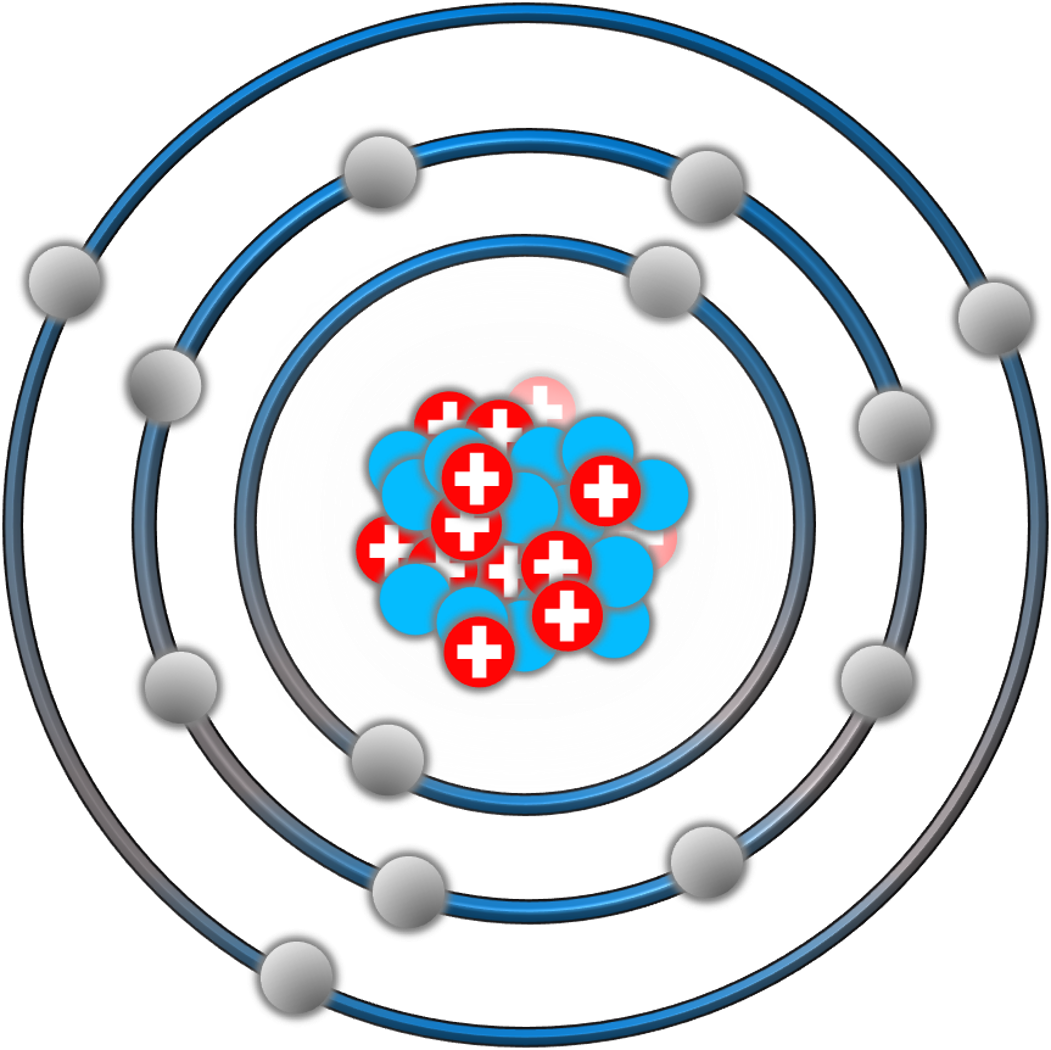
\includegraphics[width=3cm]{Images/anhminhoa/mohinhntbor.png}
		\captionof{figure}{Mô hình nguyên tử Rutherford - Bohr}
		\label{fig:mhntbo}
		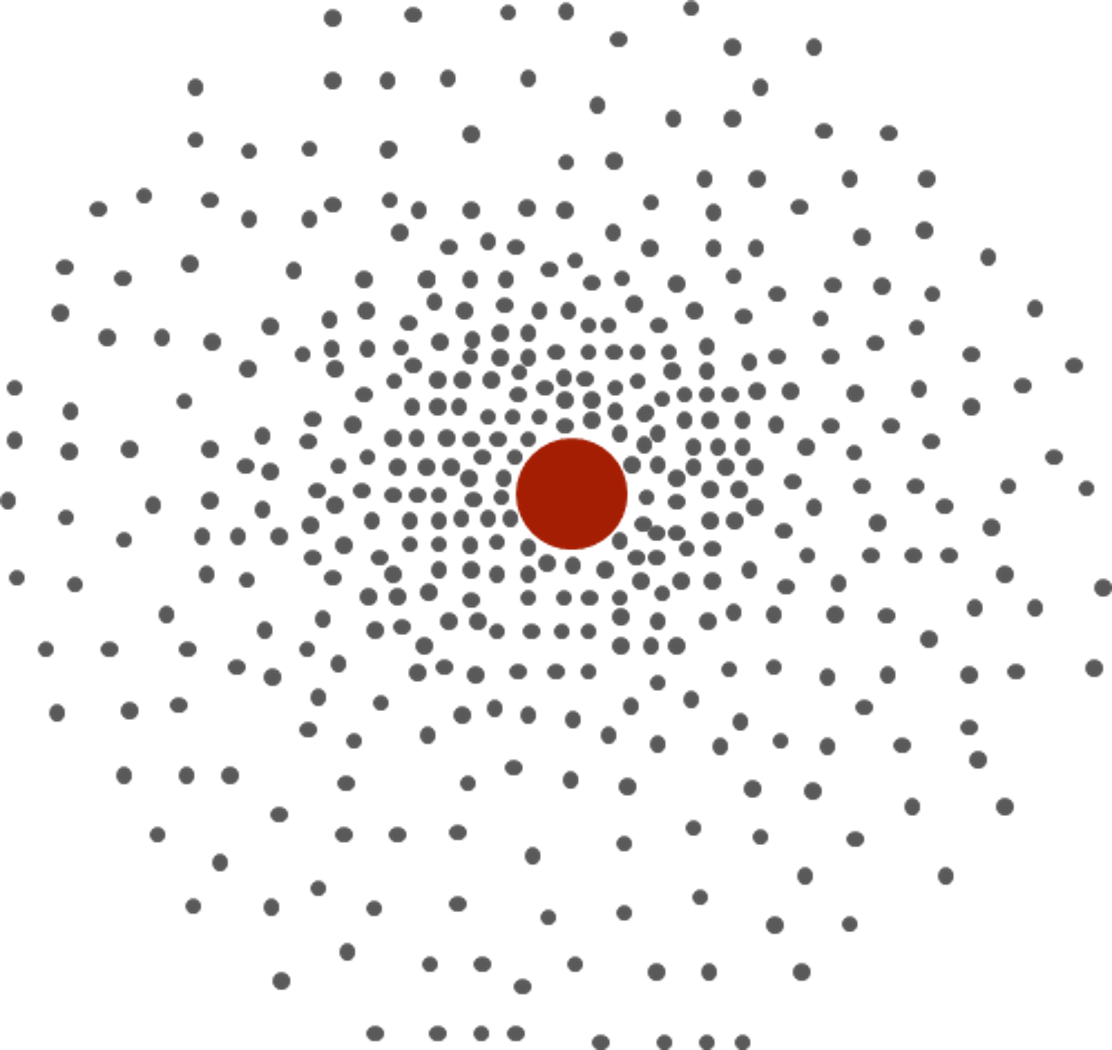
\includegraphics[width=3cm]{Images/anhminhoa/Mohinhnguyentuhiendai.png}
		\captionof{figure}{Mô hình nguyên tử hiện đại}
		\label{fig:mhnthd}
		\end{center}
\huongdan{
\begin{tabular}{|C{.25\textwidth}|L{0.65\textwidth}|}
\hline
\rowcolor{\mycolor!50!white} \multicolumn{1}{|c|}{ \sffamily\textbf{Mô hình} } & \multicolumn{1}{c|}{ \sffamily\textbf{Nội dung} } \\
\hline 
	Rutherford-Bohr &\makecell[l]{- Chưa có hạt neutron \\- Các electron quay xung quanh hạt nhân theo từng quỹ đạo\\ tròn ổn định, trong đó mỗi quỹ đạo có một mức năng lượng\\ xác định.}\\
\hline	
\makecell[c]{Hiện đại\\(Đám mây electron)} & \makecell[l]{- Đã tìm ra hạt neutron \\- Các electron chuyển độngh rất nhanh xung quanh hạt nhân\\ không theo một quỹ đạo xác định và tạo thành một đám mây\\ mang điện tích âm.}\\
\hline
\end{tabular}
}
\end{hoivadap}

\begin{emcobiet}
	Mô hình của Rutherford được gọi là mô hình mẫu hành tinh nguyên tử.
\end{emcobiet}
\subsubsection{Tìm hiểu về orbital nguyên tử}

\begin{dngsnd}
	\begin{itemize}
		\item \indam{Orbital nguyên tử} (Atomic Orbital, viết tắt $\mathrm{AO}$ ) là khu vực không gian xung quanh hạt nhân nguyên tử mà tại đó xác suất tìm thấy electron là lớn nhất (khoảng $90 \%$ ).
		\item Dựa trên sự khác nhau  về hình dạng và sự định hướng trong không gian của các orbital, người ta phân thành orbital s, orbital p, orbital d,orbital f
	\end{itemize}
\end{dngsnd}
Dưới đây là hình ảnh một số AO-s và AO-d (xem hình \ref{fig:hinhdangAO})\\
\begin{tikzpicture}
	% Định dạng cho cột của bảng
	\tikzset{%
		mynode/.style={%
		    ultra thick,
			minimum height=0.65cm,
			align=center,
			font=\sffamily
		},
		mymatrix/.style={%
			matrix of nodes,
			nodes={mynode},
			row 1/.style={%
				nodes={%
					fill=\mycolor!40!white,
					text centered,
					font=\bfseries\sffamily
				}
			},
			column 1/.style={%
				nodes={minimum width=0.25\textwidth}
			},
			column 2/.style={%
				nodes={minimum width=0.25\textwidth}
			},
			column 3/.style={%
				nodes={minimum width=0.25\textwidth}
			},
			column 4/.style={%
				nodes={minimum width=0.25\textwidth}
			}
		}
	}
	\matrix(Bang)[mymatrix]{%
	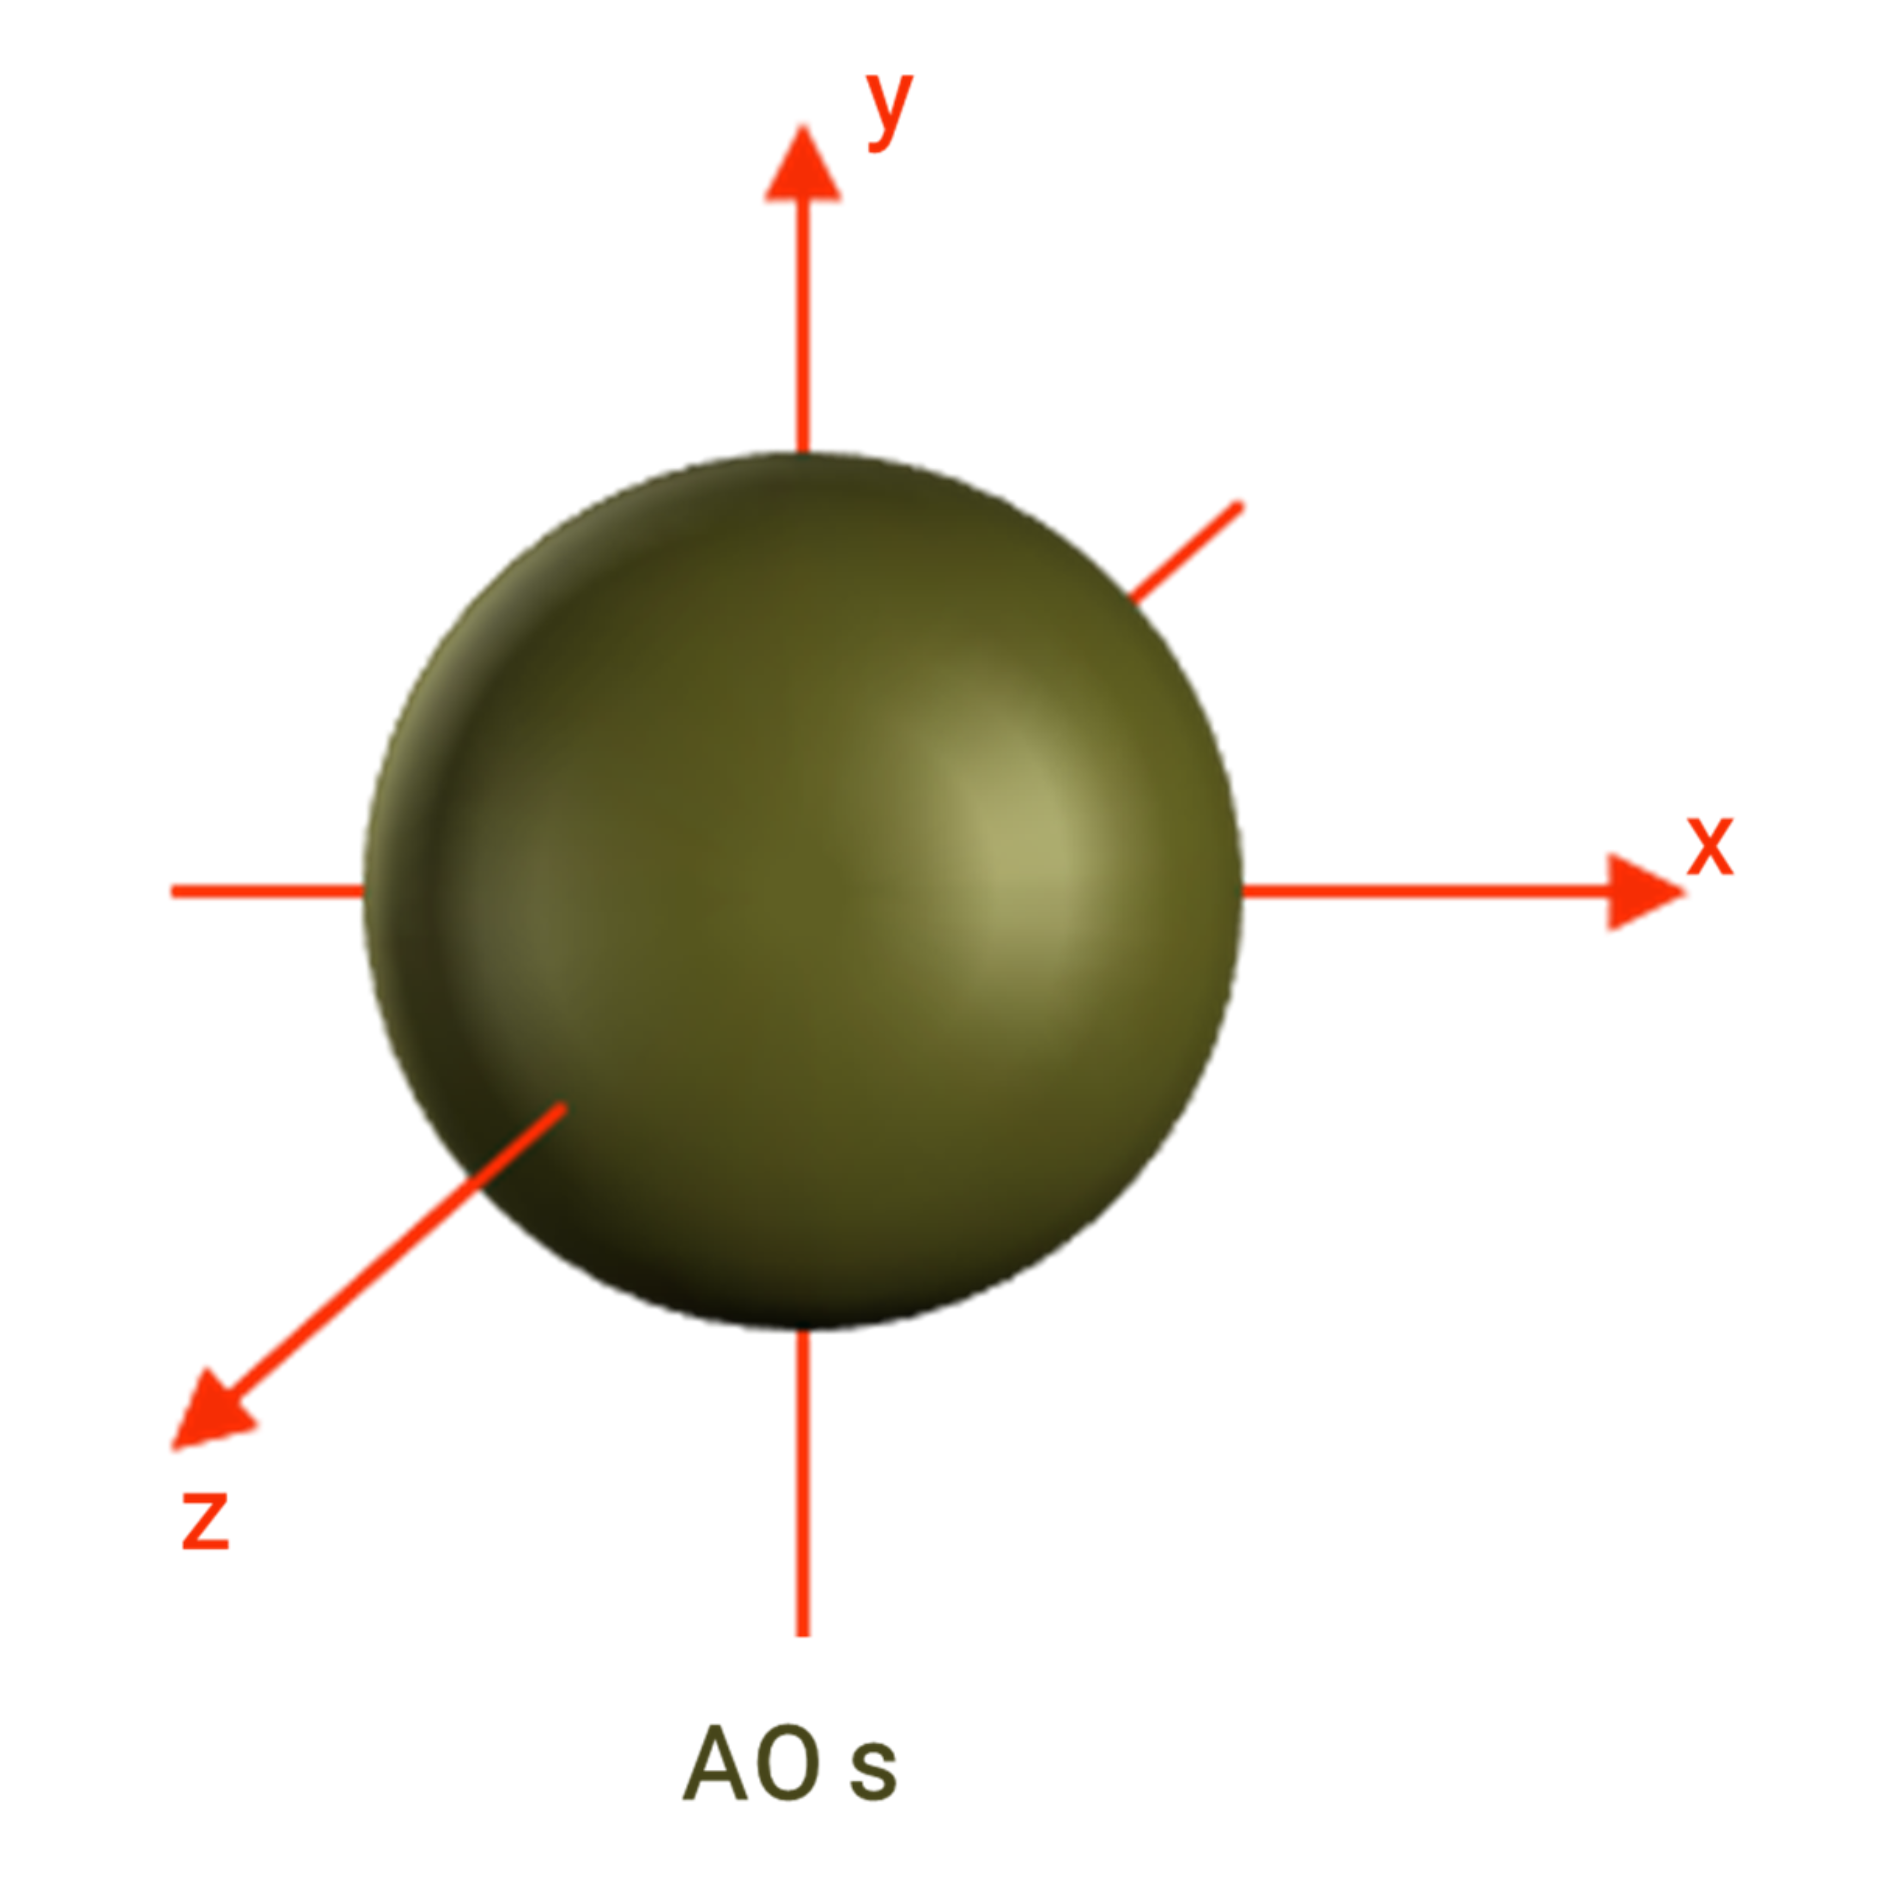
\includegraphics[width=3cm]{Images/anhminhoa/S.png}  & 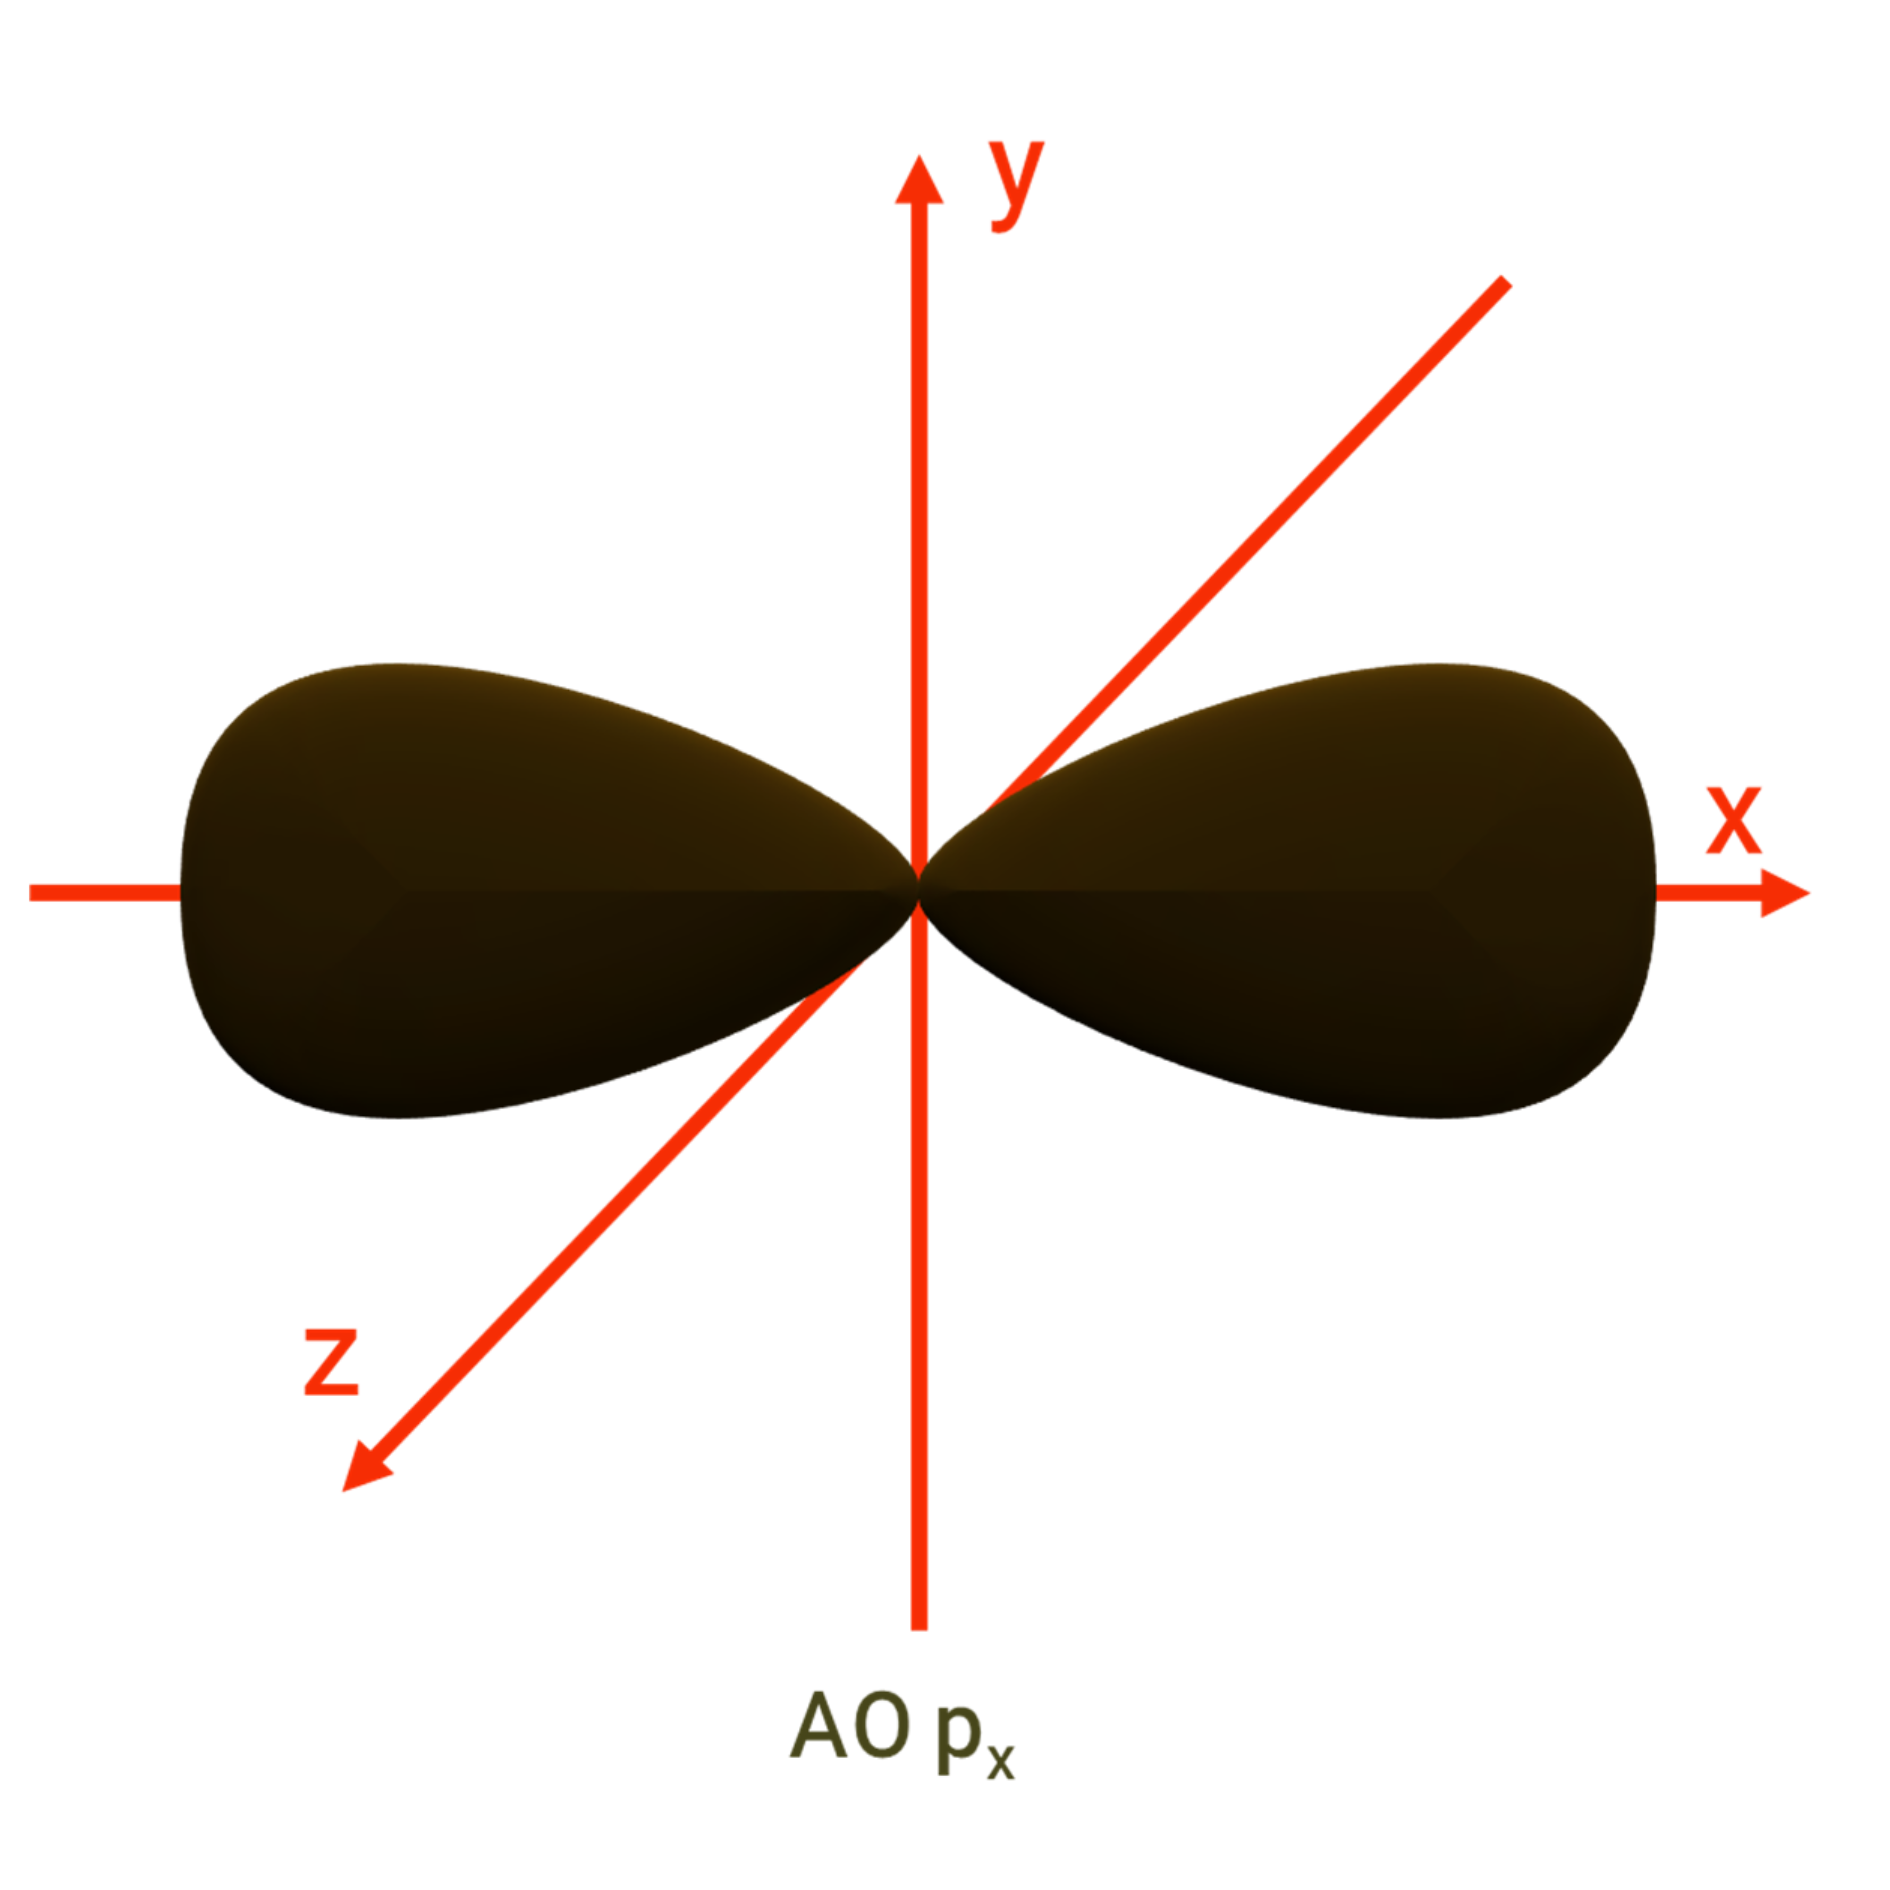
\includegraphics[width=3cm]{Images/anhminhoa/Px.png} & 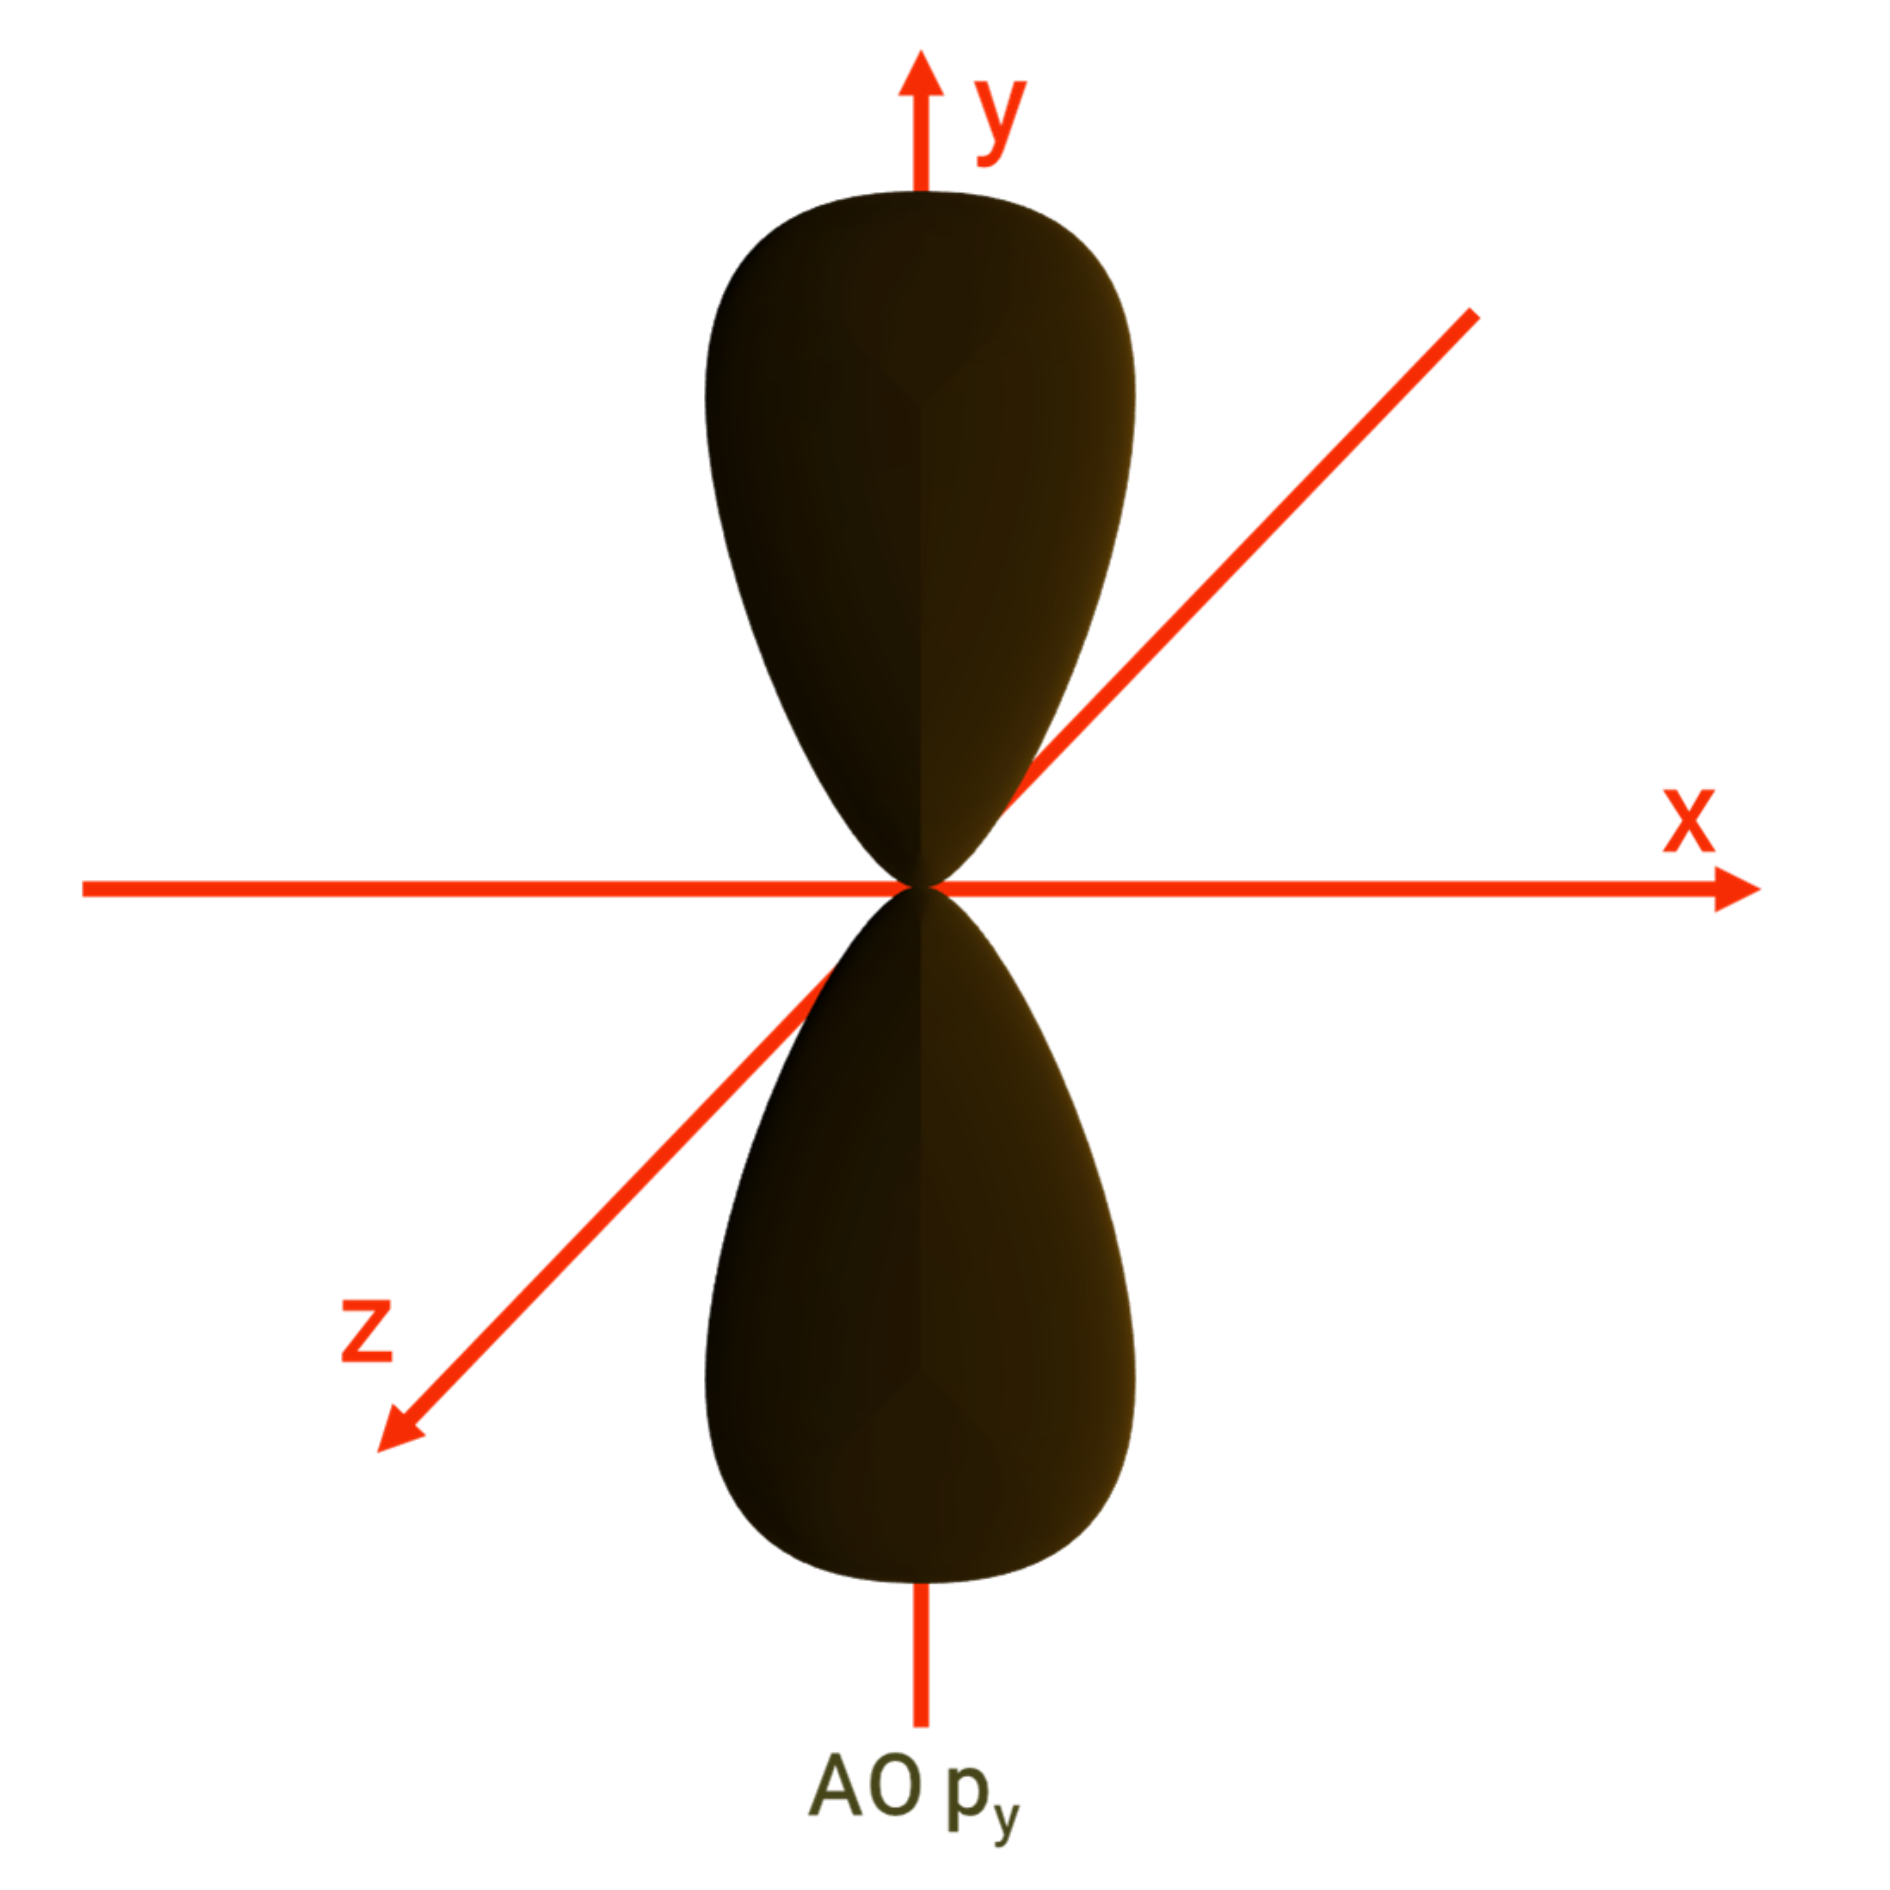
\includegraphics[width=3cm]{Images/anhminhoa/Py.png} &
	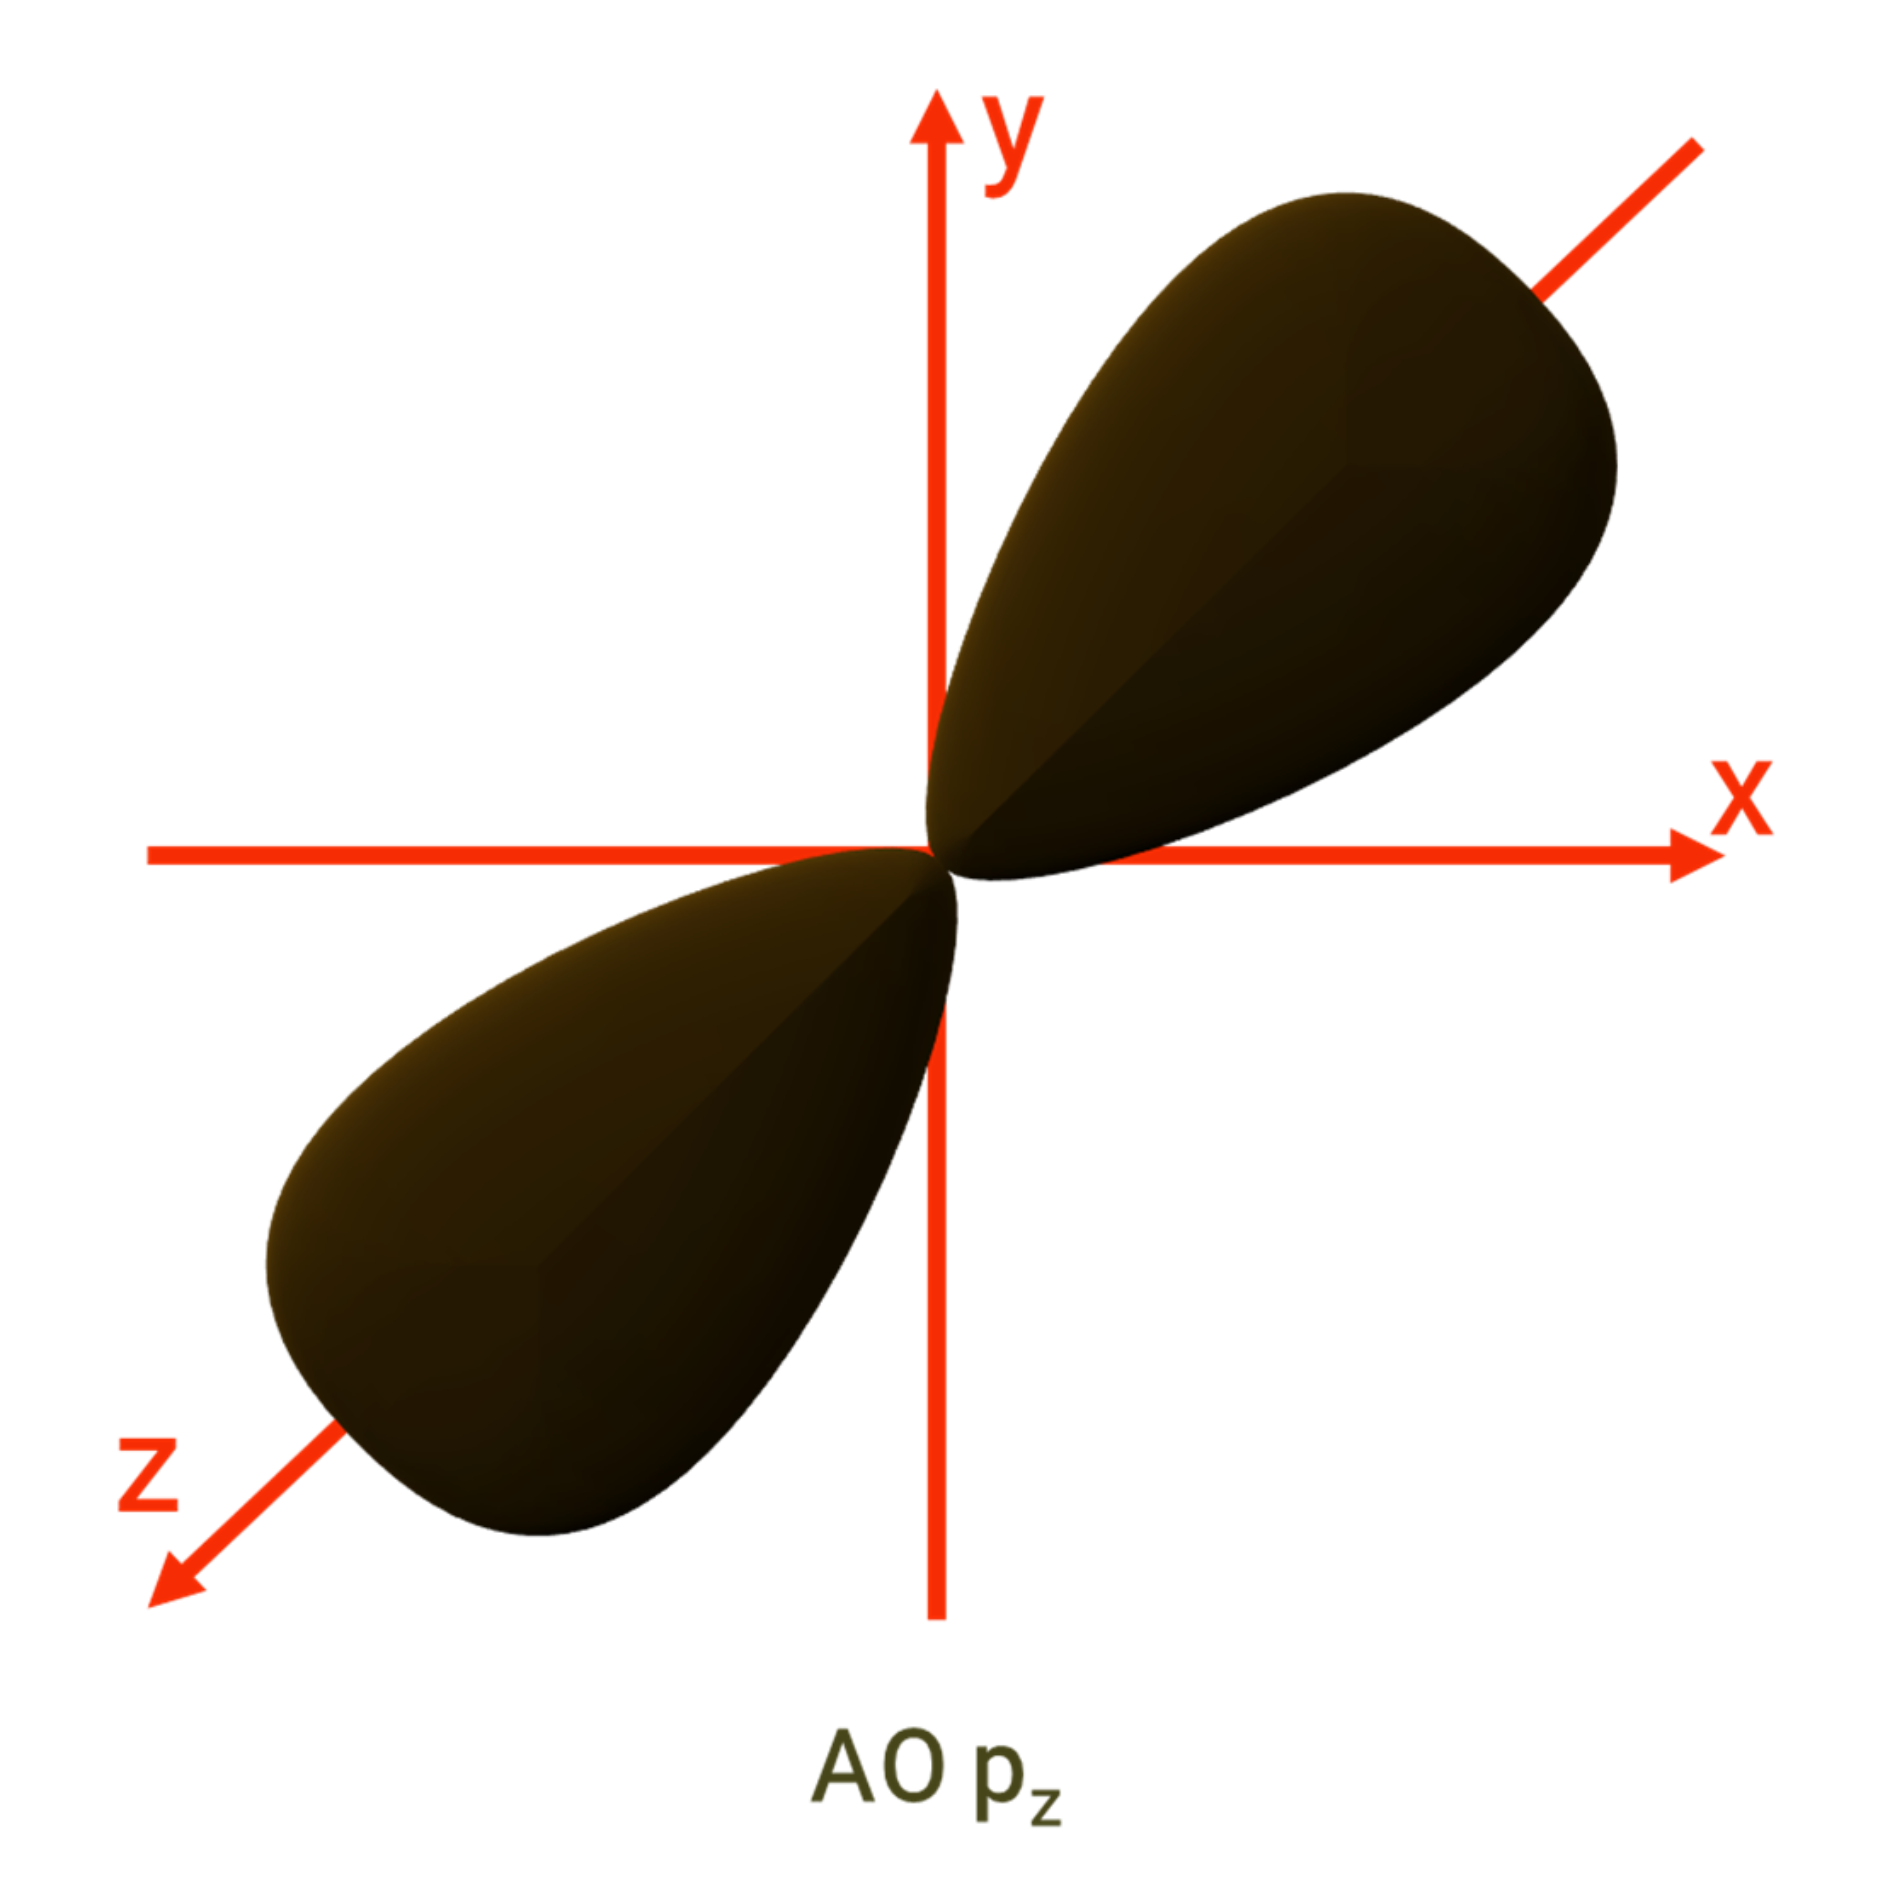
\includegraphics[width=3cm]{Images/anhminhoa/Pz.png}\\ 
	};
\end{tikzpicture}
\captionof{figure}{Hình dạng của các AO-s và AO-d}
\label{fig:hinhdangAO}
\subsection{Lớp và phân lớp electon}
\subsubsection{Lớp electron}

\begin{hoplythuyet}
	\begin{itemize}
	\item Trong nguyên tử, các electron được sắp xếp thành từng lớp ( kí hiệu lần lượt là:K,L,M,N,O,P,Q,...) và phân lớp theo mức năng lượng từ thấp đến cao.
	\item Các electron trên cùng  một lớp có mức năng lượng gần bằng nhau.
	\item Lớp electron gần hạt nhân nhất có năng lượng thấp nhất. càng xa hạt nhân năng lượng càng cao.
\end{itemize}
\end{hoplythuyet}
\begin{center}
	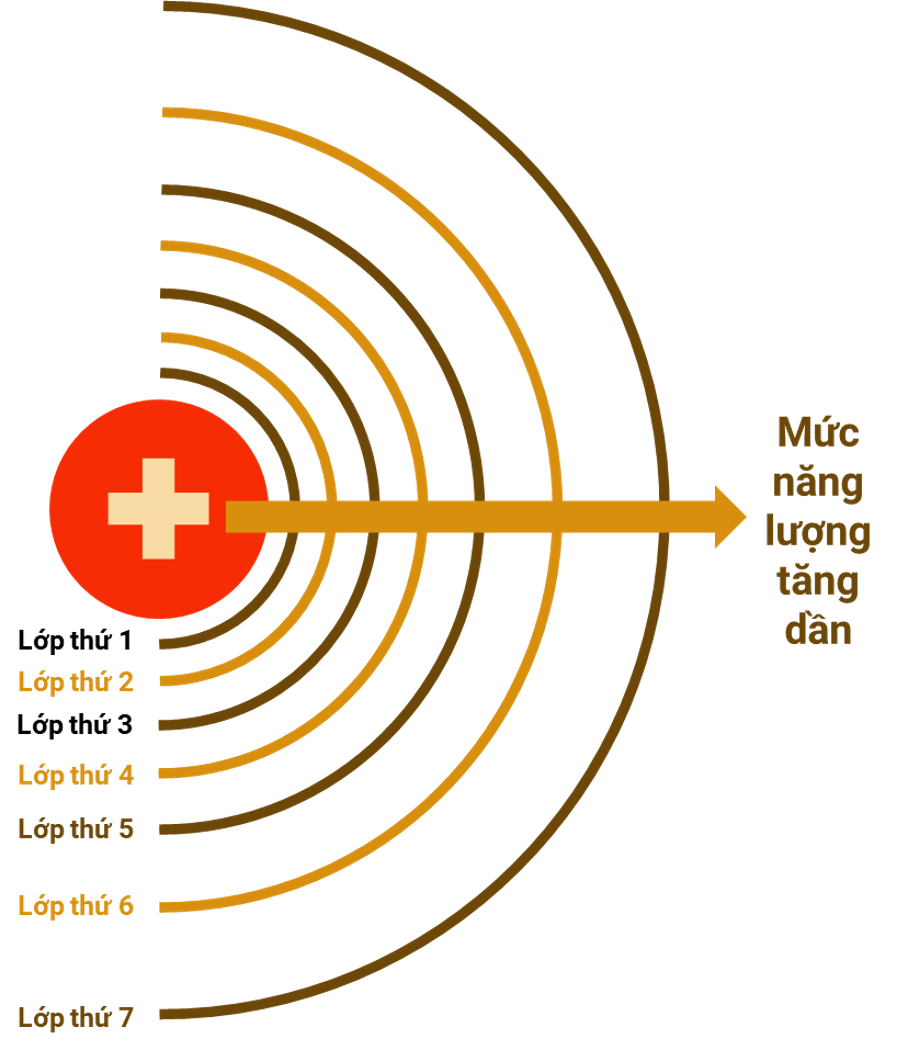
\includegraphics[height=6cm]{Images/anhminhoa/Lopelectron.png}
\end{center}
\subsubsection{Phân lớp electron}
\begin{hoplythuyet}
	\begin{itemize}
		\item Mỗi lớp electron chia thành các phân lớp ( Kí hiệu là: s, p, d, f)
		\item Các electron ở phân lớp s, p, d, f gọi là electron s, p, d, f.
		\item Các electron trên cùng một phân lớp thì có mức năng lượng bằng nhau
		\item Số phân lớp trong mỗi lớp bằng số thứ tự  của lớp đó.
	\end{itemize}
\end{hoplythuyet}

\begin{center}
%%=========Hình 4=========%%
\begin{tikzpicture}[declare function={r=3.0;}]
	\path [fill=cyan](0,0)-- (90:{r+5.6}) arc (90:0:{r+5.6}) -- cycle;
	\path [fill=violet](0,0)-- (90:{r+5.3}) arc (90:0:{r+5.3}) -- cycle;
	\path [fill=\mycolor](0,0)-- (90:{r+5}) arc (90:0:{r+5}) -- cycle;
	\path [fill=\mauphu](0,0) -- (90:{r+4.7}) arc (90:0:{r+4.7}) -- cycle;
	\path [fill=white](0,0)-- (90:{r+4.4}) arc (90:0:{r+4.4}) -- cycle;
	\path [fill=violet](0,0)-- (90:{r+3.6}) arc (90:0:{r+3.6}) -- cycle;
	\path [fill=\mycolor](0,0)-- (90:{r+3.3}) arc (90:0:{r+3.3}) -- cycle;
	\path [fill=\mauphu](0,0) -- (90:{r+3}) arc (90:0:{r+3}) -- cycle;
	\path [fill=white](0,0)-- (90:{r+2.7}) arc (90:0:{r+2.7}) -- cycle;
	\path [fill=\mycolor](0,0)-- (90:{r+2}) arc (90:0:{r+2}) -- cycle;
	\path [fill=\mauphu](0,0)-- (90:{r+1.7}) arc (90:0:{r+1.7}) -- cycle;
	\path [fill=white](0,0) -- (90:{r+1.4}) arc (90:0:{r+1.4}) -- cycle;
	\path [fill=\mauphu](0,0) -- (90:{r+.8}) arc (90:0:{r+.8}) -- cycle;
	\path [fill= white](0,0) -- (90:{r+.5}) arc (90:0:{r+.5}) -- cycle;
	\path [fill=\maunhan](0,0) -- (90:r) arc (90:0:r) -- cycle;
	\path ($(0,0)+(1.5,1.3)$) node[font=\color{white}\bfseries\sffamily,text width =2.5cm] {Hạt nhân nguyên tử};
%	\draw[%
%	decoration={%
%		text along path,
%        text={{\bfseries\sffamily H}{\bfseries\sffamily ử}{\bfseries\sffamily t} {\bfseries\sffamily n}{\bfseries\sffamily h}{\bfseries\sffamily â}{\bfseries\sffamily n} {\bfseries\sffamily n}{\bfseries\sffamily g}{\bfseries\sffamily u}{\bfseries\sffamily y}{\bfseries\sffamily ê}{\bfseries\sffamily n} {\bfseries\sffamily t}{\bfseries\sffamily ử}},
%		text align={center},
%		text color = white
%		},
%		decorate,
%		]
%		(90:{r-.4}) arc(90:0:{r-.4});
	\path 
	(0:{r+0.65}) node[font=\tiny\sffamily,below]{1s}
	(90:{r+0.65}) node[font=\tiny\sffamily,left,anchor=east]{Lớp thứ 1}
	(0:{r+1.55}) node[font=\tiny\sffamily,below]{2s}
	(90:{r+1.7}) node[font=\tiny\sffamily,left,anchor=east]{Lớp thứ 2}
	(0:{r+1.85}) node[font=\tiny\sffamily,below]{2p}
	(0:{r+2.85}) node[font=\tiny\sffamily,below]{3s}
	(0:{r+3.15}) node[font=\tiny\sffamily,below]{3p}
	(90:{r+3.15}) node[font=\tiny\sffamily,left,anchor=east]{Lớp thứ 3}
	(0:{r+3.45}) node[font=\tiny\sffamily,below]{3d}
	(0:{r+3.45}) node[font=\tiny\sffamily,below]{3d}
	(0:{r+4.55}) node[font=\tiny\sffamily,below]{4s}
	(0:{r+4.85}) node[font=\tiny\sffamily,below]{4p}
	(90:{r+5.0}) node[font=\tiny\sffamily,left,anchor=east]{Lớp thứ 4}
	(0:{r+5.15}) node[font=\tiny\sffamily,below]{4d}
	(0:{r+5.45}) node[font=\tiny\sffamily,below]{4f}
	;
\end{tikzpicture}
%%========= Hết hình4=========%
\captionof{figure}{Kí hiệu một số lớp và phân lớp trong nguyên tử}
\end{center}

\begin{center}
\begin{tikzpicture}[font=\normalsize]
	
\tikzset{%
%%Lưu tùy chọn vẽ đường tròn với tên ntdcircle	
ntdcircle/.style={%
	circle,
	fill=\maudam, % Màu và kiểu viền cho hình tròn
	inner sep=0pt,
	minimum size=.3cm % Kích thước hình tròn
},
mycircle/.pic={%
	\node[ntdcircle] at (0,0) {};
},
	%%% Đinh dạng trong 1 ô
	ntdnode/.style={%
		thick,
		anchor=center,
		align=center,
		minimum height = .4cm,
		minimum width = 2cm,
		font=\sffamily,
	},
	%%% Định dạng toàn cục
	ntdmatrix/.style={%
		matrix of nodes,
		inner sep =5pt,
		nodes in empty cells,
		fill =\mycolor!15,
		row sep=-\pgflinewidth,
		column sep=-\pgflinewidth,
		nodes={ntdnode},
		row 1/.style={%
			nodes={%
				fill=\mauphu!40!white,
				text centered,
				font=\bfseries\sffamily,
				draw=white,
%				ultra thick,
				inner sep =12pt
			}
		},
		row 2/.style={%
			nodes={%
				align=center,
				font=\bfseries\sffamily,
				inner sep =5pt,
				fill=\mauphu!20!white
			}
		},
		row 3/.style={%
			nodes={%
				align=center,
				font=\bfseries\sffamily,
				inner sep =5pt,
				fill=\mauphu!20!white
			}
		},
		row 4/.style={%
			nodes={%
				align=center,
				font=\bfseries\sffamily,
				inner sep =5pt,
				fill=\mauphu!40!white
			}
		},
		row 5/.style={%
			nodes={%
				align=center,
				font=\bfseries\sffamily,
				inner sep =5pt,
				fill=\mauphu!40!white
			}
		},
		row 6/.style={%
			nodes={%
				align=center,
				font=\bfseries\sffamily,
				inner sep =5pt,
				fill=\mauphu!20!white
			}
		},
		row 7/.style={%
			nodes={%
				align=center,
				font=\bfseries\sffamily,
				inner sep =5pt,
				fill=\mauphu!20!white
			}
		},
		row 8/.style={%
			nodes={%
				align=center,
				font=\bfseries\sffamily,
				inner sep =5pt,
				fill=\mauphu!40!white
			}
		},
		row 9/.style={%
			nodes={%
				align=center,
				font=\bfseries\sffamily,
				inner sep =5pt,
				fill=\mauphu!40!white
			}
		},
		column 1/.style={%
			nodes={%
				align=center,
				font=\bfseries\sffamily,
				inner sep =5pt
			}
		},
		column 5/.style={%
			nodes={%
				minimum width = 3.5cm,
			}
		},
	}
}

\matrix (ple) [ntdmatrix]{%
	 &  &  &  & \\
	 &  &  &  & \\
	 &  &  &  & \\
	 &  &  &  & \\
	 &  &  &  & \\
	 &  &  &  & \\
	 &  &  &  & \\
	 &  &  &  & \\
	 &  &  &  & \\
};
\fill[%
draw=white,
fill=\mauphu!60!white,
inner sep =5pt
]
(ple-1-1.north west)rectangle (ple-1-1.south east)node[anchor=center,midway,font=\bfseries\sffamily]{Lớp};
\fill[%
draw=white,
fill=\mauphu!60!white,
inner sep =5pt
]
(ple-1-1.north east)rectangle (ple-1-5.south east)node[anchor=center,midway,font=\bfseries\sffamily]{Phân lớp và số Orbital trên phân lớp};

\foreach \j/\n in {3/1s,5/2s,7/3s,9/4s}{%
	\path ([yshift=10pt]ple-\j-2.center) node[font=\sffamily] {\n};
	\foreach \i in {0}{%
		\draw 
		($(ple-\j-2.center)+(\i,0)$) pic{mycircle}
		;
	}

}

\foreach \j/\n in {5/2p,7/3p,9/4p}{%
	\path ([yshift=10pt]ple-\j-3.center) node[font=\sffamily] {\n};
	\foreach \i in {-0.35,0,.35}{%
		\draw 
		($(ple-\j-3.center)+(\i,0)$) pic{mycircle}
		;
	}
	
}

\foreach \j/\n in {7/3d,9/4d}{%
	\path ([yshift=10pt]ple-\j-4.center) node[font=\sffamily] {\n};
	\foreach \i in {-0.7,-0.35,0,.35,0.7}{%
		\draw 
		($(ple-\j-4.center)+(\i,0)$) pic{mycircle}
		;
	}
	
} 

\foreach \j in {9}{%
	\path ([yshift=10pt]ple-\j-5.center) node[font=\sffamily] {4f};
	\foreach \i in {-1.05,-0.7,-0.35,0,.35,0.7,1.05}{%
		\draw 
		($(ple-\j-5.center)+(\i,0)$) pic{mycircle}
		;
	}
} 

\foreach \x/\y/\z/\t in {20/2/3/1,40/4/5/2,20/6/7/3,40/8/9/4}{%
\fill[draw=white,fill=\mauphu!\x!white] (ple-\y-1.north west) rectangle (ple-\z-1.south east) node [anchor=center,midway,font=\bfseries\sffamily]{n=\t};
}

\end{tikzpicture}
\end{center}
\subsubsection{Cấu hình electron}
\paragraph{Nguyên lý vững bền}
\begin{hoplythuyet}
\GSND[\bfseries][\faTrello][\maunhan]{Nguyên lý vững bền}\\
\lq\lq Ở trạng thái cơ bản,các electron trong nguyên tử chiếm lần lượt những Orbital có mức năng lượng từ thấp đến cao.\rq\rq
\end{hoplythuyet}
%%%%%%%%%==============Nguyên lý vững bền==================%%%%%%%%%%
%\begin{center}
%		\begin{tikzpicture}[font=\Large,declare function={d=1.5cm; r={sqrt(2)/8 *d};}]
%			\tikzset{%a
%			ntdnode/.style={%
%				minimum height=0.65cm,
%				align=center,
%				font=\sffamily\bfseries,
%				minimum width =d,
%				minimum height =d,
%%				draw=cyan,
%			},
%			ntdmatrix/.style={%
%				matrix of nodes,
%				inner sep=5pt,
%				nodes in empty cells,
%%				fill=\mycolor!75,
%				row sep=-\pgflinewidth,
%				column sep=-\pgflinewidth,
%				nodes={ntdnode},
%				rounded corners=4pt,
%			},
%			line/.style={%
%			\maunhan!50!red,
%			arrows = {-Stealth},
%			line width=3pt,
%			}
%		}
%
%		\matrix (NLVB) [ntdmatrix] {%
%			 &  &  &  \\
%			 &  &  &  \\
%			 &  &  &  \\
%			 &  &  &  \\
%			 &  &  &  \\
%			 &  &  &  \\
%			 &  &  &  \\
%			 &  &  &  \\
%	};
%	
%	\draw (NLVB-1-1.south west) arc(135:315:r)
%	--(NLVB-1-1.east) arc(135:-45:r)--(NLVB-2-1.north east)
%	--(NLVB-2-1.south west) arc(135:315:r)--(NLVB-1-2.east) arc(135:-45:r)--(NLVB-2-2.north east)
%	--(NLVB-3-1.south west) arc(135:315:r)--(NLVB-2-2.east) arc(135:-45:r)--(NLVB-3-2.north east)
%	--(NLVB-4-1.south west) arc(135:315:r)--(NLVB-2-3.east) arc(135:-45:r)--(NLVB-3-3.north east)
%	--(NLVB-5-1.south west) arc(135:315:r)--(NLVB-3-3.east) arc(135:-45:r)--(NLVB-4-3.north east) 
%	--(NLVB-6-1.south west) arc(135:315:r)--(NLVB-3-4.east) arc(135:-45:r)--(NLVB-4-4.north east)
%	--(NLVB-7-1.south west) arc(135:315:r)--(NLVB-4-4.east) arc(135:-45:r)--(NLVB-5-4.north east)
%	;
%	
%	\foreach \h/\t/\n in {1/1/1,2/1/2,2/2/3,3/2/4,3/3/5,4/3/6,4/4/7,5/4/8}{%
%	\draw[line] (NLVB-\h-\t.north east)--(NLVB-\n-1.south west);	
%	}
%
%	
%	\foreach \i in {1,2,...,8}{%
%		\foreach \j in {1}{%
%			\path(NLVB-\i-\j.center) node[font=\bfseries\Large\sffamily,anchor=center]{\ntdshape{\i \color{\mycolor}{s}}}	;
%		}
%	}
%	\foreach \i in {2,3,...,7}{%
%		\foreach \j in {2}{%
%			\path(NLVB-\i-\j.center) node[font=\bfseries\Large\sffamily,anchor=center]{\ntdshape{\i \color{\maudam}{p}}}	;
%		}
%	}
%	\foreach \i in {3,4,...,6}{%
%		\foreach \j in {3}{%
%			\path(NLVB-\i-\j.center) node[font=\bfseries\Large\sffamily,anchor=center]{\ntdshape{\i \color{\maunhan}{d}}}	;
%		}
%	}
%	\foreach \i in {4,5}{%
%		\foreach \j in {4}{%
%			\path(NLVB-\i-\j.center) node[font=\bfseries\Large\sffamily,anchor=center]{\ntdshape{\i \color{\mauphu}{f}}}	;
%		}
%	}
%		\end{tikzpicture}
%	\captionof{figure}{Quy tắc Klechkowski }
%	\label{fig:Klechkowski}
%\end{center}

\begin{emcobiet}
		Các electron sắp sếp theo thứ tự mức năng lượng từ thấp đến cao được mô phỏng theo \indam{Quy tắc Klechkowski} (Xem hình \ref{fig:Klechkowski})\\
		Theo quy tắc này ta có trật tự mức năng lượng electron như sau:\\
		\begin{center}
		\boxct[\maunhan][3pt][\bfseries\sffamily][arc is angular]{1s,2s,2p,3p,4s,3d,4p,5s,4d,5p,6s,$\ldots$}
		\end{center}
		\begin{center}
			\begin{tikzpicture}[font=\Large,declare function={d=1.5cm; r={sqrt(2)/8 *d};}]
				\tikzset{%a
					ntdnode/.style={%
						minimum height=0.65cm,
						align=center,
						font=\sffamily\bfseries,
						minimum width =d,
						minimum height =d,
						%				draw=cyan,
					},
					ntdmatrix/.style={%
						matrix of nodes,
						inner sep=5pt,
						nodes in empty cells,
%						fill=\mycolor,
						row sep=-\pgflinewidth,
						column sep=-\pgflinewidth,
						nodes={ntdnode},
						rounded corners=4pt,
					},
					line/.style={%
						\maunhan!50!red,
						arrows = {-Stealth},
						line width=3pt,
					}
				}
				
				\matrix (NLVB) [ntdmatrix] {%
					&  &  &  \\
					&  &  &  \\
					&  &  &  \\
					&  &  &  \\
					&  &  &  \\
					&  &  &  \\
					&  &  &  \\
					&  &  &  \\
				};
				
				\draw (NLVB-1-1.south west) arc(135:315:r)
				--(NLVB-1-1.east) arc(135:-45:r)--(NLVB-2-1.north east)
				--(NLVB-2-1.south west) arc(135:315:r)--(NLVB-1-2.east) arc(135:-45:r)--(NLVB-2-2.north east)
				--(NLVB-3-1.south west) arc(135:315:r)--(NLVB-2-2.east) arc(135:-45:r)--(NLVB-3-2.north east)
				--(NLVB-4-1.south west) arc(135:315:r)--(NLVB-2-3.east) arc(135:-45:r)--(NLVB-3-3.north east)
				--(NLVB-5-1.south west) arc(135:315:r)--(NLVB-3-3.east) arc(135:-45:r)--(NLVB-4-3.north east) 
				--(NLVB-6-1.south west) arc(135:315:r)--(NLVB-3-4.east) arc(135:-45:r)--(NLVB-4-4.north east)
				--(NLVB-7-1.south west) arc(135:315:r)--(NLVB-4-4.east) arc(135:-45:r)--(NLVB-5-4.north east)
				;
				
				\foreach \h/\t/\n in {1/1/1,2/1/2,2/2/3,3/2/4,3/3/5,4/3/6,4/4/7,5/4/8}{%
					\draw[line] (NLVB-\h-\t.north east)--(NLVB-\n-1.south west);	
				}
				
				
				\foreach \i in {1,2,...,8}{%
					\foreach \j in {1}{%
						\path(NLVB-\i-\j.center) node[font=\bfseries\Large\sffamily,anchor=center]{\ntdshape{\i \color{\mycolor}{s}}}	;
					}
				}
				\foreach \i in {2,3,...,7}{%
					\foreach \j in {2}{%
						\path(NLVB-\i-\j.center) node[font=\bfseries\Large\sffamily,anchor=center]{\ntdshape{\i \color{\maudam}{p}}}	;
					}
				}
				\foreach \i in {3,4,...,6}{%
					\foreach \j in {3}{%
						\path(NLVB-\i-\j.center) node[font=\bfseries\Large\sffamily,anchor=center]{\ntdshape{\i \color{\maunhan}{d}}}	;
					}
				}
				\foreach \i in {4,5}{%
					\foreach \j in {4}{%
						\path(NLVB-\i-\j.center) node[font=\bfseries\Large\sffamily,anchor=center]{\ntdshape{\i \color{\mauphu}{f}}}	;
					}
				}
			\end{tikzpicture}
			\captionof{figure}{Quy tắc Klechkowski }
			\label{fig:Klechkowski}
		\end{center}
\end{emcobiet}

\paragraph{Nguyên lý pauli}

\begin{hoplythuyet}
	\indam{Nguyên lí Pauli:} Mỗi orbital chỉ chứa tối đa 2 electron và có chiều tự quay ngược nhau.
\end{hoplythuyet}

\begin{tikzpicture}
	\path (0,0) node[anchor=center](eghepdoi) {\Eghepdoi}
	      (eghepdoi.east) node [xshift=-5pt,anchor=west]{:\ \indam{Electron ghép đôi}}
	;
	
	\path (0,-1) node[anchor=center](edocthan) {\Edocthan}
	(edocthan.east) node [xshift=-5pt,anchor=west]{:\ \indam{Electron độc thân}}
	;
\end{tikzpicture}
\paragraph{Xác định số AO và số electron tối đa trong một phân lớp và trong mỗi lớp}

\begin{tikzpicture}[font=\normalsize,declare function={d=2.6cm;r=.9cm;}]
	\tikzset{%a
		ntdnode/.style={%
			align=center,
			font=\sffamily\bfseries,
			minimum width =d,
			minimum height =r,
			draw=white,
			anchor =center,
			fill=\mycolor!75,
		},
		ntdmatrix/.style={%
			matrix of nodes,
			inner sep=5pt,
			nodes in empty cells,
%			fill=\mycolor!15,
			row sep=-\pgflinewidth,
			column sep=-\pgflinewidth,
			nodes={ntdnode},
%			rounded corners=4pt,
		column 1/.style={%
			nodes={%
				align=center,
				font=\bfseries\sffamily,
				inner sep =5pt,
				minimum width =1.2cm
			}
		},
		row 1/.style={%
			nodes={%
				align=center,
				font=\color{white}\bfseries\sffamily,
				inner sep =5pt,
				minimum height =2cm,
				fill=\maudam!85
			}
		},		
		column 4/.style={%
			nodes={%
				minimum width =3.4cm
			}
		},
		column 5/.style={%
			nodes={%
				minimum width =3.8cm
			}
		},
		column 6/.style={%
			nodes={%
				minimum width =3.6cm
			}
		},	
	},
		line/.style={%
			\maunhan!50!red,
			arrows = {-Stealth},
			line width=3pt,
		}
	}
	\matrix (soelectron) [ntdmatrix] {%
	n	& Tên lớp & \makecell{Tên \\phân lớp} & \makecell{Số AO\\ trong mỗi\\ phân lớp} & \makecell{Số e \\tối đa trong\\ mỗi phân lớp} & \makecell[c]{Số e \\tối đa trong\\ một lớp} \\
		&  & s & 1 & 2 &  \\
		&  & s & 1 & 2 &  \\
		&  & p & 3 & 6 &  \\
		&  & s & 1 & 2 &  \\
		&  & p & 3 & 6 &  \\
		&  & d &  5& 10& \\
		&  & s & 1 & 2 &  \\
		&  & p & 3 & 6 &  \\
		&  & d & 5 & 10&  \\
		&  & f & 7 & 14&  \\
	n	&  & $n^2$ &   & &  \\
	};
\foreach \i/\j/\k in {2/2/1,3/4/2,5/7/3,8/11/4,12/12/n}{%
\path[draw=white,fill=\mycolor!75](soelectron-\i-1.north west) rectangle (soelectron-\j-1.south east)node[midway,anchor=center]{\indam{\k}};
}	

\foreach \i/\j/\k in {2/2/K,3/4/L,5/7/M,8/11/N}{%
	\path[draw=white,fill=\mycolor!75](soelectron-\i-2.north west) rectangle (soelectron-\j-2.south east)node[midway,anchor=center]{\indam[black]{\k}};
}

\foreach \i/\j/\k in {2/2/$2=2\cdot1^2$,3/4/$8=2\cdot2^2$,5/7/$18=2\cdot3^2$,8/11/$32=2\cdot4^2$,12/12/$2n^2$}{%
	\path[draw=white,fill=\mycolor!75](soelectron-\i-6.north west) rectangle (soelectron-\j-6.south east)node[midway,anchor=center]{\indam[black]{\k}};
}
\path[draw=white,fill=\mycolor!75](soelectron-12-2.north west) rectangle (soelectron-12-5.south east)node[midway,anchor=center]{\indam[black]{$n^2$}};	
\end{tikzpicture}
\paragraph{Quy tắc hund}
\begin{hoplythuyet}
	\lq \lq Trong cùng một phân lớp chưa bão hòa, các electron sẽ phân bố vào các AO sao cho số e độc thân là tối đa\rq \rq
\end{hoplythuyet}


\begin{hoivadap}
	Trong các trường hợp dưới đây trường hợp nào các electron điền e vào các orbital theo các nguyên lý và quy tắc đã học
\begin{myenum}
	\item
	\begin{adjustbox}{valign=m}
		\begin{tikzpicture}[declare function={x=.896cm;l=1.2;}]   
			\path(0:{0*x}) node [anchor=center](dxy) {\Eghepdoi}
			(0:{1*x}) node [anchor=center](dyz) {\Eghepdoi}
			(0:{2*x}) node [anchor=center](dzz) {\Eghepdoi}
			(0:{3*x}) node [anchor=center](pxxyy) {\Eghepdoi}
			(0:{4*x}) node [anchor=center](pxz) {\Edocthan};
			\path (0:{5*x}) node [anchor=center,transform canvas={shift={(10pt,-3pt)}}](ssss) {\Edocthan[\maunhan]};
			\path([xshift=15pt]ssss.south)node[anchor=north]{$4s^1$};
			\path([xshift=3.2pt]dzz.south)node[anchor=north]{$3d^{9}$};
		\end{tikzpicture}
	\end{adjustbox}
	\item
	\begin{adjustbox}{valign=m}
		\begin{tikzpicture}[declare function={x=.896cm;l=1.2;}]  
			\path(0:{0*x}) node [anchor=center](dxy) {\Eghepdoi}
			(0:{1*x}) node [anchor=center](dyz) {\Eghepdoi}
			(0:{2*x}) node [anchor=center](dzz) {\Edocthan}
			(0:{3*x}) node [anchor=center](pxxyy) {\Edocthan}
			(0:{4*x}) node [anchor=center](pxz) {\Edocthan};
			\path (0:{5*x}) node [anchor=center,transform canvas={shift={(10pt,-3pt)}}](ssss) {\Eghepdoi[\maunhan]};
			\path([xshift=15pt]ssss.south)node[anchor=north]{$4s^2$};
			\path([xshift=3.2pt]dzz.south)node[anchor=north]{$3d^{9}$};
		\end{tikzpicture}
	\end{adjustbox}
	\item
	\begin{adjustbox}{valign=m}
		\begin{tikzpicture}[declare function={x=.896cm;l=1.2;}]  
			\path(0:{0*x}) node [anchor=center](SSS) {\Eghepdoi}
			(0:{1*x}) node [anchor=center,transform canvas={shift={(10pt,3pt)}}](p) {\Eghepdoi}
			(0:{2*x}) node [anchor=center,transform canvas={shift={(10pt,3pt)}}](pp) {\Eghepdoi}
			(0:{3*x}) node [anchor=center,transform canvas={shift={(10pt,3pt)}}](ppp) {\AOtrong};
			\path([xshift=5pt]SSS.south)node[anchor=north]{$3s^2$};
			\path([xshift=14pt]pp.south)node[anchor=north]{$3p^{4}$};
		\end{tikzpicture}
	\end{adjustbox}
\end{myenum}
\end{hoivadap}

\begin{notegsnd}
%%%%=================== Phan lop d========================%%%%%%%%%%%%%
\begin{tikzpicture}[declare function={d=.6cm;r={d/2.4};}]
		\tikzset{
			eghepdoi/.pic={
				\draw[arrows={-Stealth}, line width=1pt, \maudam]
				(0,0)--(0,d);
				\draw[arrows={-Stealth}, line width=1pt, \maudam]
				(r,d)--(r,0);
			},
			edocthan/.pic={
				\draw[arrows={-Stealth}, line width=1pt, \maudam]
				(0,0)--(0,d);
			},
			echuaghepdoi/.pic={
				\draw[arrows={-Stealth}, line width=1pt, \maudam]
				(0,0)--(0,d);
				\path[arrows={-Stealth}, line width=1pt, \maudam]
				(r,d)--(r,0);
			}
		}
%%%%%%%%%%%%%%%%%%%%%%%Cấu hình 3d bão hòa%%%%%%%%%%%%%%%%%%%%%%%%%%%%%%
	\matrix (pld)[%
	matrix of nodes,
	nodes={%
		draw= \maudam,
		thick,
		minimum height =.8cm,
		minimum width = .8cm,
		anchor = center,
		align =center,
		inner sep =3pt,
	},
	nodes in empty cells,
	row sep=-\pgflinewidth,
	column sep=-\pgflinewidth,
	]{%
		& & & &\\
	};
%%%%%%%%%%%%%%%%%%%%%%%%%%%%%%%%%%%%%%%%%%%%%%%%%%%%%%%%%%%%%%%%%%%%%%%%%%%%%%%%	
	\begin{scope}[transform canvas={xshift=-3.7pt,yshift=-8.7pt}]
	\foreach \x in {1,2,3,4,5}{
		\draw(pld-1-\x.center) pic {eghepdoi};
	}
\end{scope}	

\path (pld.south) node[anchor=north,font=\small] {Cấu hình bão hòa (bền)};
	\end{tikzpicture}
%%%%%%%%%%%%%%%%%%%%%%%%Cấu hình 3d Bán bão hòa=======================%%%%%%%%%%%%%%%%%%%%%%%%	
	\begin{tikzpicture}[declare function={d=.60cm;r={d/2.4};}]
	\tikzset{
		eghepdoi/.pic={
			\draw[arrows={-Stealth}, line width=1pt, \maudam]
			(0,0)--(0,d);
			\draw[arrows={-Stealth}, line width=1pt, \maudam]
			(r,d)--(r,0);
		},
		edocthan/.pic={
			\draw[arrows={-Stealth}, line width=1pt, \maudam]
			(0,0)--(0,d);
		},
		echuaghepdoi/.pic={
			\draw[arrows={-Stealth}, line width=1pt, \maudam]
			(0,0)--(0,d);
			\path[arrows={-Stealth}, line width=1pt, \maudam]
			(r,d)--(r,0);
		}
	}
	%%%%%%%%%%%%%%%%%%%%%%%%%%%%%%%%%%%%%%%%%%%%%%%%%%%%%%%%%%%%%%%%%%%%%%%%%%%%%%%%
	\matrix (pld)[%
	matrix of nodes,
	nodes={%
		draw= \maudam,
		thick,
		minimum height =.8cm,
		minimum width = .8cm,
		anchor = center,
		align =center,
		inner sep =3pt,
	},
	nodes in empty cells,
	row sep=-\pgflinewidth,
	column sep=-\pgflinewidth,
	]{%
		& & & &\\
	};
	%%%%%%%%%%%%%%%%%%%%%%%%%%%%%%%%%%%%%%%%%%%%%%%%%%%%%%%%%%%%%%%%%%%%%%%%%%%%%%%%	
	\begin{scope}[transform canvas={xshift=-0.5pt,yshift=-8.7pt}]
		\foreach \x in {1,2,3,4,5}{
			\draw(pld-1-\x.center) pic {edocthan};
		}
	\end{scope}	
\path (pld.south) node[anchor=north,font=\small] {Cấu hình bán bão hòa (bền)};	
\end{tikzpicture}	
%%%%%%%%%%%%%%%%%%%%%%%%Cấu hình 3d chưa bão hòa=======================%%%%%%%%%%%%%%%%%%%%%%%%	
\begin{tikzpicture}[declare function={d=.60cm;r={d/2.4};}]
	\tikzset{
		eghepdoi/.pic={
			\draw[arrows={-Stealth}, line width=1pt, \maudam]
			(0,0)--(0,d);
			\draw[arrows={-Stealth}, line width=1pt, \maudam]
			(r,d)--(r,0);
		},
		edocthan/.pic={
			\draw[arrows={-Stealth}, line width=1pt, \maudam]
			(0,0)--(0,d);
		},
		echuaghepdoi/.pic={
			\draw[arrows={-Stealth}, line width=1pt, \maudam]
			(0,0)--(0,d);
			\path[arrows={-Stealth}, line width=1pt, \maudam]
			(r,d)--(r,0);
		}
	}
	%%%%%%%%%%%%%%%%%%%%%%%%%%%%%%%%%%%%%%%%%%%%%%%%%%%%%%%%%%%%%%%%%%%%%%%%%%%%%%%%
	\matrix (pld)[%
	matrix of nodes,
	nodes={%
		draw= \maudam,
		thick,
		minimum height =.8cm,
		minimum width = .8cm,
		anchor = center,
		align =center,
		inner sep =3pt,
	},
	nodes in empty cells,
	row sep=-\pgflinewidth,
	column sep=-\pgflinewidth,
	]{%
		& & & &\\
	};
	%%%%%%%%%%%%%%%%%%%%%%%%%%%%%%%%%%%%%%%%%%%%%%%%%%%%%%%%%%%%%%%%%%%%%%%%%%%%%%%%	
	\begin{scope}[transform canvas={xshift=-3pt,yshift=-8.7pt}]
		\foreach \x in {1,2,3}{
			\draw(pld-1-\x.center) pic {eghepdoi};
		}
	\end{scope}	
	\begin{scope}[transform canvas={xshift=-0.5pt,yshift=-8.7pt}]
			\foreach \x in {4,5}{
			\draw(pld-1-\x.center) pic {edocthan};
		}
	\end{scope}
	\path (pld.south) node[anchor=north,font=\small] {Cấu hình chưa bão hòa (kém bền)};	
\end{tikzpicture}
\GSND[][\faBell][\maunhan]{Một số cấu hình đặc biệt: ${}_{29}Cu$	và ${}_{24}Cr$}
\begin{itemize}
\item Cấu hình của ${}_{29}Cu$ theo quy luật sẽ là $[Ar]3d^94s^2$ [\footnote{Cách viết cấu hình thu gọn}].Tuy nhiên một electron từ phân lớp 4s tham gia ghép đôi với 1 e độc thân ở 3d để đạt trạng thái bão hào ở phân lớp 3d $[Ar]3d^{10}4s^1$ bền vững hơn.\\
\begin{tikzpicture}	[declare function={x=.896cm;l=1.2;}]	
	\path(0:{0*x}) node [anchor=center](dxy) {\Eghepdoi}
	(0:{1*x}) node [anchor=center](dyz) {\Eghepdoi}
	(0:{2*x}) node [anchor=center](dzz) {\Eghepdoi}
	(0:{3*x}) node [anchor=center](pxxyy) {\Eghepdoi}
	(0:{4*x}) node [anchor=center](pxz) {\Ecbghepdoi[\maunhan]}
	;
	\path([xshift=3.2pt]dzz.south)node[anchor=north]{$3d^9$};
	\begin{scope}[transform canvas={shift={(10pt,-3pt)}}]
		\path (0:{5*x}) node [anchor=center](ssss) {\Eghepdoi[\maunhan]};
		\path([xshift=3.2pt]ssss.south)node[anchor=north]{$4s^2$};
	\end{scope}
	\path(0:{9*x}) node [anchor=center](dxy1) {\Eghepdoi}
	(0:{10*x}) node [anchor=center](dyz1) {\Eghepdoi}
	(0:{11*x}) node [anchor=center](dzz1) {\Eghepdoi}
	(0:{12*x}) node [anchor=center](pxxyy1) {\Eghepdoi}
	(0:{13*x}) node [anchor=center](pxz1) {\Eghepdoi[\maunhan]}
	;
	\path([xshift=3.2pt]dzz1.south)node[anchor=north]{$3d^{10}$};
	\begin{scope}[transform canvas={shift={(10pt,-3pt)}}]
		\path (0:{14*x}) node [anchor=center](ssss1) {\Ecbghepdoi[\maunhan]};
		\path([xshift=3.2pt]ssss1.south)node[anchor=north]{$4s^1$};
	\end{scope}
%	\draw[->,arrows={-Stealth}, line width=1pt]([xshift=16pt]ssss.east)--(dxy1.west);
	\draw[->,arrows={-Stealth}, line width=1pt]([xshift=16pt]ssss.east)--(dxy1.west);
	\draw[\maunhan,->,arrows={-Stealth}, line width=1pt]([xshift=.6cm,yshift=-2pt]ssss.north) .. controls+(90:l) and +(90:l) .. ([xshift=10pt]pxz.north);
\end{tikzpicture}\\
\item Cấu hình của ${}_{24}Cr$:Tương tự như vậy cấu hình đúng của Cr là $[Ar]3d^{5}4s^{1}$ (cấu hình bán bão hòa) thay vì $ [Ar]3d^{4}4s^{2}$\\
\begin{tikzpicture}	[declare function={x=.896cm;l=1.2;}]	
	\path(0:{0*x}) node [anchor=center](dxy) {\Edocthan}
	(0:{1*x}) node [anchor=center](dyz) {\Edocthan}
	(0:{2*x}) node [anchor=center](dzz) {\Edocthan}
	(0:{3*x}) node [anchor=center](pxxyy) {\Edocthan}
	(0:{4*x}) node [anchor=center](pxz) {\AOtrong[\maunhan][.633cm]}
	;
	\path([xshift=3.2pt]dzz.south)node[anchor=north]{$3d^4$};
	\begin{scope}[transform canvas={shift={(10pt,-3pt)}}]
		\path (0:{5*x}) node [anchor=center](ssss) {\Eghepdoi[\maunhan]};
		\path([xshift=3.2pt]ssss.south)node[anchor=north]{$4s^2$};
	\end{scope}
	\path(0:{9*x}) node [anchor=center](dxy1) {\Edocthan}
	(0:{10*x}) node [anchor=center](dyz1) {\Edocthan}
	(0:{11*x}) node [anchor=center](dzz1) {\Edocthan}
	(0:{12*x}) node [anchor=center](pxxyy1) {\Edocthan}
	(0:{13*x}) node [anchor=center](pxz1) {\Edocthan[\maunhan]}
	;
	\path([xshift=3.2pt]dzz1.south)node[anchor=north]{$3d^{5}$};
	\begin{scope}[transform canvas={shift={(10pt,-3pt)}}]
		\path (0:{14*x}) node [anchor=center](ssss1) {\Ecbghepdoi[\maunhan]};
		\path([xshift=3.2pt]ssss1.south)node[anchor=north]{$4s^1$};
	\end{scope}
	%	\draw[->,arrows={-Stealth}, line width=1pt]([xshift=16pt]ssss.east)--(dxy1.west);
	\draw[->,arrows={-Stealth}, line width=1pt]([xshift=16pt]ssss.east)--(dxy1.west);
	\draw[\maunhan,->,arrows={-Stealth}, line width=1pt]([xshift=.6cm,yshift=-2pt]ssss.north) .. controls+(90:l) and +(90:l) .. ([xshift=5pt]pxz.north);
\end{tikzpicture}
\end{itemize}
\end{notegsnd}
\paragraph{Cách viết cấu hình electron nguyên tử}
\begin{dngsnd}
	Cấu hình electron nguyên tử biểu diễn sự phân bố electron trong vỏ nguyên tử trên các phân lớp thuộc các lớp khác nhau.
	
	%%=========Hình 1=========%%
	\begin{center}
		\begin{tikzpicture}[declare function={b=4cm;r=5cm;l=5cm;}]
			\tikzstyle{mynote} = [%
			anchor=center,
			rectangle,
			inner sep =3pt,
			draw =\mycolor, 
			ultra thick,
			rounded corners =4pt,
			text width =3cm,
			align=center,
			font=\large\color{\mycolor!50!black}\bfseries\sffamily
			]
			\tikzstyle{line} = [%
			->,
			arrows={-Stealth},
			line width = 3pt,
			\maudam
			]
			%%%%%%%%%%%%%%%%%%%%%%%%%%%%%%%%%%%%%%%%%%%%%%%%%%%%%%%%%%%%%%%%%
			\path (0,0) coordinate (A) 			node[anchor=center,font=\fontsize{45pt}{6pt}\fontfamily{qag}\selectfont](cauhinh){\indam{1s$^{2}$}}
			  (cauhinh)--++(0:r) coordinate (B)
			  ([yshift=-3pt]cauhinh)--++(180:l) coordinate (C)
			  ([xshift=3pt]cauhinh)--++(-90:b) coordinate (D);
				\path (B) node [mynote,text width =3cm](soe) {Số e trên phân lớp};
				\draw[line] (soe) -- (cauhinh);
			\path (C) node [mynote,text width =2.5cm](Stt) {Số thứ tự lớp};
			\draw[line](Stt)--([yshift=-8pt]cauhinh) ;
				\path (D) node [mynote,text width =2.5cm](KH) {Kí hiệu phân lớp};			
			\draw[line](KH.north)--([xshift=3pt]cauhinh.south);
		\end{tikzpicture}
	\end{center}
	%%========= Hết hình1=========%
\end{dngsnd}
	
\GSND[\bfseries\sffamily][\faArchive][\maunhan]{Quy ước:}
\begin{itemize}
	\item Số thứ tự electron dduocj ghi bằng chữ số (1,2,3,\ldots)
	\item Phân lớp được ghi  bằng các chữ cái thường (s, p, d, f)
	\item Số electron trong một phân lớp được ghi bằng số ở phía trên bên phải của phân lớp ($s^2$,$p^6$,\ldots)
\end{itemize}

\begin{hoplythuyet}
\GSND[\bfseries\sffamily][\faBook][\maunhan]{Cách viết cấu hình electron}	
	\begin{enumerate}[label=\protect{\bfseries\sffamily Bước \arabic*:},wide=0.65cm,leftmargin=0.65cm]
		\item Xác định số electron của nguyên tử
		\item Các electron được phân bố theo thứ tự các AO có mức năng lượng tăng dần, theo các nguyên lý và quy tắc phân bố electron trong nguyên tử
		\item Viết cấu hình electron theo thứ tự các phân lớp trong một lớp và theo thứ tự của các lớp electron.
	\end{enumerate}
\end{hoplythuyet}

\paragraph{Đặc điểm cấu hình electron lớp ngoài cùng của các nguyên tố nhóm A}

\begin{hoplythuyet}
	\begin{itemize}
		\item Các nguyên tử có \indam{1,2,3 electron} ở lớp ngoài cùng thường là các \indam{kim loại} có khuynh hướng nhường đi 1,2,3 electron đó.
		\item Các nguyên tử có \indam{5,6,7 electron} ở lớp ngoài cùng thường là các \indam{phi kim}, có khuynh hướng nhận thêm 3,2,1 electron đó.
		\item Các nguyên tử có \indam{4 electron}  ở lớp ngoài cùng thường là các kim, loạicó thể là \indam{kim loại hoặc phi kim}.
		\item các nguyên tử có \indam{8 electron} ở lớp ngoài cùng là nguyên tử của nguyên tố \indam{khí hiếm} (trừ He có 2 electron ở lớp ngoài cùng) 
	\end{itemize}
\end{hoplythuyet}
%%%==========Nội dung file thứ 7===============%%%
\chapter{Cấu tạo nguyên tử}
\section{Thành phần nguyên tử}
\subsection{NỘI DUNG BÀI HỌC}
\subsubsection{SỰ PHÁT TRIỂN MÔ HÌNH NGUYÊN TỬ}
\begin{hoplythuyet}
\begin{minipage}[htp!]{0.5\textwidth}
Từ thời cổ Hy Lạp,nhà triết học Democritous (Đê-mô-crít) (Hình \ref{fig:Democritus})
Mọi thứ trên thế giới đều được tạo ra từ các hạt nhỏ không thể chia nhỏ được nữa được gọi là \textbf{“nguyên tử”}, có nghĩa là \textbf{“không thể thay đổi được”}
\end{minipage}
\begin{minipage}[htp!]{0.5\textwidth}
\begin{center}
		\includegraphics[width=3cm]{DEMOCRITUS}
		\captionof{figure}{Democritus (460 - 370,Hy Lạp)\label{fig:Democritus} }
\end{center}
\end{minipage}

\begin{center}
	\includegraphics[width=12cm]{Historyatom}
	\captionof{figure}{Lịch sử phát triển mô hình nguyên tử \label{fig:Historyatom} }
\end{center}
\end{hoplythuyet}
\subsubsection{Thành phần và cấu trúc của nguyên tử}
\paragraph{Thành phần}
\begin{hoplythuyet}
	Nguyên tử gồm hạt nhân chứa proton, neutron và vỏ nguyên tử chứa electron.
	\begin{center}
		\includegraphics[width=9cm]{mohinhnguyentu}
		\captionof{figure}{Mô hình nguyên tử}
	\end{center}
\end{hoplythuyet}
\paragraph{Sự tìm ra electron}
\ntd{Thí nghiệm khám phá tia âm cực của Thomson}\\
Năm 1897, J.J.Thomson (Tôm-xơn, người Anh) thực hiện thí nghiệm phóng điện qua không khí loãng đã phát hiện ra chùm tia phát ra từ cực âm.(xem hình \ref{fig:tiaamcuc} ) và link video bằng mã QR ở bên dưới.\\ 
\begin{minipage}{0.6\textwidth}
\begin{center}
\includegraphics[width=9cm]{TNTHOMSON}\\
\captionof{figure}{Thí nghiệm của Thomson}
\label{fig:tiaamcuc}
\end{center}
\end{minipage}
\hfill
\begin{minipage}{0.3\textwidth}
\begin{tikzpicture}
\path (0,0)  node (QRCODE) {\qrcode[height=2.0cm]{https://youtu.be/y2uswXtC5O8}}
(QRCODE.south) node[anchor=north]{(\fmmfamily Các bạn  dùng ~\rotatebox{-15}{\faMobile}~quét mã QR để xem video TN nhé!)}
;
\end{tikzpicture}
\end{minipage}
\begin{hoivadap}
	Vai trò của lớp bột huỳnh quang trong thí nghiệm ở hình \ref{fig:tiaamcuc}
	\huongdan{\taodongke{10}}
\end{hoivadap}
%
\begin{hoivadap}
Quan sát Hình \ref{fig:tiaamcuc} và video , giải thích vì sao tia âm cực bị hút về cực dương của trường điện.
	\huongdan{\taodongke{10}}
\end{hoivadap}
%
\begin{hoivadap}
	Nếu đặt một chong chóng nhẹ trên đường đi của tia âm cực thì chong chóng sẽ quay. Từ hiện tượng đó, hãy nêu kết luận về tính chất của tia âm cực.
	\huongdan{\taodongke{5}}
\end{hoivadap}
\newpage
\vspace*{6pt}
\begin{emcobiet}
	 Mô hình Thomson còn gọi là mô hình \lq\lq bánh pudding mận".Theo Thomson:
	\begin{enumerate}
		\item Nguyên tử là quả cầu mang điện tích dương, bên trong chứa các êlectron.
	    \item Nguyên tử trung hòa về điện.
	\end{enumerate}
\end{emcobiet}
%
%
\paragraph{Sự khám phá hạt nhân nguyên tử}
\ntd{Tìm hiểu thí nghiệm của Rutherford}\\
Năm 1911, E. Rutherford (Ro-dơ-pho, người Niu Di-lân) thực hiện thí nghiệm bắn phá lá vàng rất mỏng bằng chùm hạt $ \alpha $ \footnote{Hạt $\alpha$ : hạt nhân helium, mang điện tích dương.} (xem hình \ref{fig:hinh4})
\begin{center}
		\includegraphics[width=9cm]{TNRUTHERFORT}\\
		\captionof{figure}{Thí nghiệm của Rutherford}
		\label{fig:hinh4}
\end{center}
%
\begin{center}
\includegraphics[width=9cm]{KQTN}\\
\captionof{figure}{Kết quả thí nghiệm của Rutherford}
\label{fig:hinh5}
\end{center}
%
\begin{hoivadap}
	Quan sát hình \ref{fig:hinh4}, cho biết các hạt $\alpha$ có đường đi như thế nào. Dựa vào Hình \ref{fig:hinh5} , giải thich kết quả thí nghiệm thu được.
	\huongdan{\taodongke{5}}
\end{hoivadap}
\vspace*{6pt}
\begin{hoplythuyet}
	{\bfseries{Kết luận}}
	\begin{itemize}
	\item Nguyên tử có cấu tạo rỗng, gồm hạt nhân ở trung tâm và lớp vỏ là các electron chuyển động xung quanh hạt nhân.
	\item Nguyên tử trung hoà về điện: số đơn vị điện tích dương của hạt nhân bằng số đơn vị điện tích âm của các electron trong nguyên tử.
	\end{itemize}
\end{hoplythuyet}
\paragraph{Cấu tạo hạt nhân nguyên tử}
\begin{center}
	\includegraphics[width=9cm]{CAUTAOHATNHAN}\\
	\captionof{figure}{Thành phần của hạt nhân}
	\label{fig:hinh6}
\end{center}
\begin{hoivadap}
	Quan sát hình \ref{fig:hinh6} và kết hợp SGK , các bạn hãy nêu thành phần của hạt nhân
\end{hoivadap}
\begin{hoplythuyet}
	Proton, neutron và electron là các hạt cấu tạo nên nguyên tử.
\end{hoplythuyet}
\begin{tongket}
	Thành phần cấu tạo của nguyên tử gồm:
\begin{itemize}
	\item  Hạt nhân (nucleus): ở tâm của nguyên tử, chứa các proton mang điện tích dương và các neutron không mang điện.
	\item Vỏ nguyên tử: chứa các electron mang điện tích âm, chuyển động rất nhanh xung quanh hạt nhân.
	\item Trong nguyên tử, số proton bằng số electron nên nguyên tử trung hoà điện.
	\item Khối lượng của electron rất nhỏ, không đáng kể so với khối lượng của proton hay neutron nên khối lượng của nguyên tử tập trung hầu hết ở hạt nhân.
\end{itemize}
\end{tongket}


\begin{longtable}{|c|c|c|c|c|c|}
		\caption{\indam[\maunhan]{Khối lượng, điện tích của các loại hạt cấu tạo nên nguyên tử}}
		\label{tab:table1}\\
\hline
\rowcolor{dnxanh!25} \indam[dnxanh]{Hạt} & \indam[dnxanh]{Kí hiệu} & $\begin{array}{c}\text {\indam[dnxanh]{Khối lượng} } \\
		\text {\indam[dnxanh]{(kg)}  }\end{array}$ & \indam[dnxanh]{Khối lượng (amu)} & $\begin{array}{c}\text { \indam[dnxanh]{Điện tích} } \\
		\text { \indam[dnxanh]{(C)} }\end{array}$ & $\begin{array}{l}\text { \indam[dnxanh]{Điện tích} } \\
		\text { \indam[dnxanh]{tương đối} }\end{array}$ \\
\hline\endhead
\rowcolor{dnvang!15} Proton & $p$ & $1,672 \cdot 10^{-27}$ & $\approx 1$ & $1,602 \cdot 10^{-19}$ & +1 \\
\hline
\rowcolor{dnvang!15} Neutron & $\mathrm{n}$ & $1,675 \cdot 10^{-27}$ & $\approx 1$ & 0 & 0 \\
\hline\rowcolor{dnvang!15} Electron & e & $9,109 \cdot 10^{-31}$ & $\begin{array}{c}
		~ \\
		\dfrac{1}{1837} \approx 0,00055\\
		~ \\
	\end{array}$ & $-1,602 \cdot 10^{-19}$ & -1 \\
	\hline
	\end{longtable}
\paragraph{KíCH THƯỚC VÀ KHỐI LƯợNG NGUYÊN TỬ}
\begin{center}
	\includegraphics[width=9cm]{ktnt}\\
	\captionof{figure}{So sánh kích thước hạt nhân , nguyên tử}
	\label{fig:hinh7}
\end{center}
\begin{notegsnd}
		\begin{itemize}
\item Đơn vị kích thước thường dùng của nguyên tử là Angstron ($ A^0 $) hoặc nano mét (nm)			
	$$1 \mathrm{~nm}=10^{-9}~\mathrm{m} ; 1 A^0=10^{-10}~\mathrm{~m} ; 1 \mathrm{~nm}=10 A^0; 1 A^0=10^{2}~\mathrm{pm}$$
	\begin{center}
	\tcbox[width=5cm,colframe=\maunhan]{$ \dfrac{d_{\text{NT}}}{d_{\text{hạt nhân}}}\approx \dfrac{10^{-10}}{10^{-14}} \approx 10^4~\mathrm{\text{lần}} $}
	\end{center}
		\item Đơn vị của khối lương nguyên tử là amu (atomic mass unit),
		$$
		1 \mathrm{amu}=1,6605 \times 10^{-27} \mathrm{~kg} \text {. }
		$$
		\item Đơn vi của điện tích các hạt cơ bản là $\mathrm{e}_0$ (điện tích nguyên tố),
		$$
		1 \mathrm{e}_0=1,602 \times 10^{-19} \mathrm{C} \text {. }
		$$
	\end{itemize}
\end{notegsnd}
\newpage
\vspace*{3pt}

\ntd{BÀI TẬP TRẮC NGHIỆM}:
\begin{dangntd}{LÝ THUYẾT VỀ CẤU TẠO NGUYÊN TỬ}
\giaibaitap{Phương pháp giải}
\begin{itemize}
	\item Nắm vững về cấu tạo nguyên tử
	\item Nắm vững kết quả thí nghiệm của Thomson,Rutherford
\end{itemize}
\end{dangntd}
\Opensolutionfile{ansbook}[DAPAN/BTTLH10CO102tachLG]
\Opensolutionfile{ans}[DAPAN/BTTLH10CO102]
\begin{ex}[1]
	Các hạt cơ bản của hầu hết các nguyên tử là?
	\choice
{%
electron
}
{%
	electron và proton
}
{%
 proton và notron
}
{%
\True electron, proton và notron
}
%\sodongkeex[5]
\huongdan{

}
\end{ex}


\begin{ex}[1]
	Hạt nhân của hầu hết các nguyên tử gồm có?
	\choice
	{%
		electron
	}
	{%
		electron và proton
	}
	{%
	\True proton và notron
	}
	{%
		 electron, proton và notron
	}
%\sodongkeex[5]
\huongdan{
	
}
\end{ex}

\begin{ex}[2]
Trong thí nghiệm của Thomson, phát biểu nào sau đây sai với kết quả thí nghiệm ta quan sát được?
	\choice
{%
 Tia âm cực là các chùm hạt electron di chuyển từ cực âm sang cực dương
}
{%
	Tia âm cực là chùm hạt mang điện tích âm
}
{%
\True	Tia âm cực bị lệch về phía bản cực âm của nguồn điện
}
{%
	Tia âm cực bị lệch hướng khi ta đặt nó trong từ trường
}
%\sodongkeex[5]
\huongdan{
	
}
\end{ex}

\begin{ex}[2]
Theo mô hình bánh pudding mận của Thomson, phát biểu nào sau đây là đúng?
\choice
{%
Nguyên tử có cấu tạo rỗng gồm hạt nhân mang điện tích dương và vỏ là các electron chuyển động xung quanh hạt nhân.
}
{%
Nguyên tử có cấu tạo rỗng gồm hạt nhân mang điện tích dương và vỏ là các electron chuyển dộng xung quanh hạt nhân theo những quỹ đạo có kích thước và năng lượng cố định
}
{%
\True	nguyên tử bao gồm các electron nằm rải rác trong một đám mây hình cầu mang điện tích dương.
}
{%
	các electron  quay quanh hạt nhân không theo một quỹ đạo xác định, mà chúng tạo thành các đám mây điện tích mà tại đó xác suất tìm thấy electron là lớn nhất
}
%\sodongkeex[5]
\huongdan{
	
}
\end{ex}
\begin{ex}[2]
Cho các phát biểu sau:
\begin{enumerate}[(1)]
\item Tất cả các hạt nhân nguyên tử đều được cấu tạo từ các hạt proton và neutron.
\item Khối lượng nguyên tử tập trung phần lớn ở lớp vỏ.
\item Trong nguyên tử, số electron bằng số proton.
\item Trong hạt nhân nguyên tử, hạt mang điện là proton và electron.
\item Trong nguyên tử, hạt electron có khối lượng không đáng kể so với các hạt còn lại.
\end{enumerate}
Số phát biểu đúng là
\choice
{%
	1
}
{%
\True 2
}
{%
3
}
{%
4
}
\huongdan{%
Phát biểu đúng là:
Trong hạt nhân nguyên tử, hạt mang điện là proton và electron.\\
Trong nguyên tử, hạt electron có khối lượng không đáng kể so với các hạt còn lại
}

\end{ex}

\begin{ex}[2]
Điều nào sau đây đúng theo mô hình nguyên tử của Thomson?
\choice
{%
Nguyên tử không trung hòa về điện
}
{%
\True Nguyên tử là quả cầu mang điện tích dương có chứa các êlectron bên trong
}
{%
Điện tích âm và điện tích dương trong nguyên tử có độ lớn bằng nhau
}
 {%
 Không có điều nào ở trên
 }
%\sodongkeex[5]
\huongdan{
	
}
\end{ex}


\begin{ex}[3]
	Trong hiện tượng xả điện qua khí ở áp suất thấp, sự tỏa sáng màu trong ống xuất hiện là kết quả của:
	\choice
	{% 
\True va chạm giữa các hạt mang điện được phát ra từ cực âm và nguyên tử của khí
	}
{% 
	va chạm giữa các electron khác nhau của các nguyên tử trong khí
}
{% 
	kích thích các electron trong các nguyên tử
}	
{% 
va chạm giữa các nguyên tử của khí
}	
%\sodongkeex[5]
\huongdan{
	
}	
\end{ex}

\begin{ex}[2]
Mô hình đầu tiên về nguyên tử được đưa ra bởi:
\choice
{%
N. Bohr
}
{% 
	E. Goldstein
}
{% 
	Rutherford
}
{% 	
\True J.J. Thomson
}
%\sodongkeex[5]
\huongdan{
	
}
\end{ex}

\begin{ex}[2]
Nếu đường kính của nguyên tử khoảng $10^2 \mathrm{pm}$ thì đường kính của hạt nhân khoảng
\choice
{%
$10^2 \mathrm{pm}$
}
{%
$10^{-4} \mathrm{pm}$
}
{%
\True	$10^{-2} \mathrm{pm}$
}
{
$10^4 \mathrm{pm}$
}
%\sodongkeex[5]
\huongdan{
	
}
\end{ex}
\Closesolutionfile{ans}
\Closesolutionfile{ansbook}


\newpage
\giaibaitap{BÀI TẬP TỰ LUẬN}
\Opensolutionfile{ansbt}[DAPAN/BT_H10C0102]
\begin{btex}[2]
	Trong thí nghiệm của Rutherford, khi sử dụng các hạt alpha (ion $\mathrm{He}^{2+}$, kí hiệu là $\mathrm{a}$ ) bắn vào lá vàng thì:
	\begin{itemize}
	\item Hầu hết các hạt a xuyên thẳng qua lá vàng.
	\item Một số ít hạt a bị lệch quỹ đạo so với ban đầu.
	\item Một số rất ít hạt a bị bật ngược trở lại.
	\end{itemize}
	Từ kết quả này, em có nhận xét gì về cấu tạo nguyên tử?
	\loigiai{
	Trong thí nghiệm của Rutherford, khi sử dụng các hạt alpha (ion $\mathrm{He}^{2+}$, kí hiệu là a) bắn vào lá vàng thì:
	\begin{itemize}
	\item Hầu hết các hạt a xuyên thẳng qua lá vàng chứng tỏ nguyên tử có cấu tạo rỗng.
	\item Một số ít hạt a bị lệch quỹ đạo so với ban đầu chứng tỏ hạt nhân nguyên tử cùng điện tích dương như hạt hạt alpha (ion $\mathrm{He}^{2+}$, kí hiệu là $ \alpha $).
	\item Một số rất ít hạt a bị bật ngược trở lại chứng tỏ kích thước hạt nhân nhỏ hơn rất nhiều so với kích thước của nguyên tử và khối lượng nguyên tử tập trung chủ yếu ở hạt nhân.
	\end{itemize}

}
\end{btex}

\begin{btex}[2]
Viết lại bảng sau vào vở và điền thông tin còn thiếu vào các ô trống:\\
\begin{tabular}{|c|c|c|c|c|c|c|}
\rowcolor{dnxanh!25} 
\hline \indam[dnxanhdam]{Nguyên tố} & \indam[dnxanhdam]{Kí hiệu} & \color{dnxanhdam} {$\mathbf{Z}$} & \indam[dnxanhdam]{Số e} & \indam[dnxanhdam]{Số p} & \indam[dnxanhdam]{Số n} & \indam[dnxanhdam]{Số khối} \\
\rowcolor{dnvang!25} 
\hline \indam[dnxanhdam]{Carbon} & $\mathrm{C}$ & 6 & 6 & $?$ & 6 & $?$ \\
\rowcolor{dnvang!25} 
\hline \indam[dnxanhdam]{Nitrogen} & $\mathrm{N}$ & 7 & $?$ & 7 & $?$ & 14 \\
\rowcolor{dnvang!25} 
\hline \indam[dnxanhdam]{Oxygen} & $\mathrm{O}$ & 8 & 8 & $?$ & 8 & $?$ \\
\rowcolor{dnvang!25} 
\hline \indam[dnxanhdam]{Sodium (natri)} & $\mathrm{Na}$ & 11 & $?$ & 11 & $?$ & 23 \\
\rowcolor{dnvang!25}
\hline \indam[dnxanhdam]{Aluminium (nhôm)} & $\mathrm{Al}$ & $?$ & 13 & $?$ & $?$ & 27 \\
\hline
\end{tabular}
\huongdan{
\taodongke{5}
}
\end{btex}

\Closesolutionfile{ansbt}

\newpage
\begin{dangntd}{Bài tập về khối lượng, kích thước nguyên tử}	
	\giaibaitap{Phương pháp giải}\\
	\tieumuc{Các công thức liên quan khối lượng}
	\begin{itemize}
		\item $ m _{\text{nguyên tử}=m_{p}+m_{n} + m_{e} } $ (tính chính xác); $ m _{\text{nguyên tử}} \approx  m_{p} + m_{n} \approx m_{\text{hạt nhân}} $ (tính gần đúng)
		\item Khối lượng tính ra kg của 1 nguyên tử carbon-12 là $ 19,926 . 10^{27}~\mathrm{kg}$.
		\item 1 amu được định nghĩa bằng $\dfrac{1}{12}$ khối lượng 1 nguyên tử carbon-12:
		\item$1 \mathrm{amu}=\dfrac{19,926 \cdot 10^{-27} \mathrm{~kg}}{12}=1,661 \cdot 10^{-27} \mathrm{~kg}$
		\item$1 \mathrm{mol}$ chứa $ 6,02.10^{23} $ nguyên tử, phân tử, ion.
	\end{itemize}
	\tieumuc{Các công thức liên quan kích thước}
	\begin{itemize}
		\item Thể tích của hình cầu:
		$ V=\dfrac{4}{3}\pi r^3 $
		\item Phần trăm thể tích các nguyên tử trong tinh thể $ = \dfrac{V_{\text{các nguyên tử}}}{V_{\text{tinh thể}}}\cdot 100\% $
		\item Một số đơn vị đo: 
		$\left\{\begin{array}{l}
			1~\mathrm{nm} = 10^{-9}~\mathrm{m}\\
			1~\mathrm{A^{0}} = 10^{-10}~\mathrm{m}\\
			1~\mathrm{pm} = 10^{-12}~\mathrm{m}	
		\end{array}\right.$
	\end{itemize}
\end{dangntd}
\begin{vdm}{Ví dụ mẫu}
\end{vdm}

%Câu 1: Khối lượng của nguyên tử magnesium là $39,8271 \cdot 10^{-27} \mathrm{~kg}$. Khối lượng của magnesium theo amu là
%A. 23,978
%B. $66,133 \cdot 10^{-51}$.
%C. 24,000 .
%D. $23,985 \cdot 10^{-3}$.

\begin{vdex}[2]	
	Khối lượng của nguyên tử magnesium là $39,8271 \cdot 10^{-27} \mathrm{~kg}$. Khối lượng của magnesium theo amu là
	\choice
	{%
		\True $ 23,978 $
	}
	{%
		$66,133 \cdot 10^{-51}$
	}
	{%
		$23,985 \cdot 10^{-3}$
	}
	{%
		$ 24,000 $
	}
	\huongdan{
		
	}	
\end{vdex}

\begin{vdex}[2]
	Khối lượng tuyệt đối của một nguyên tử oxygen bằng $26,5595.10^{-27} \mathrm{~kg}$. Hãy tính khối lượng nguyên tử (theo amu) và khối lượng mol nguyên tử (theo g) của nguyên tử này.
	\loigiai
	{%
		$
		1 \mathrm{amu}=1,661 \cdot 10^{-27} \mathrm{~kg}
		$\\
		
		
		Khối lượng của nguyên tử oxygen theo amu là:
		$
		\dfrac{26,5595 \cdot 10^{-27}}{1,661 \cdot 10^{-27}} \approx 15,99~ \mathrm{amu}
		$\\
		
		$1 \mathrm{mol}$ chứa $ 6,02.10^{23} $ nguyên tử\\
		$\Rightarrow$ Khối lượng mol của oxygen là  $=26,5595.10^{-24}.6,02.10^{23}= 15,99~ \mathrm{gam} $
		
	}
\end{vdex}

%Câu 3: Nguyên tử helium có 2 proton, 2 neutron và 2 electron. Khối lượng của các electron chiếm baoo nhiêu $\%$ khối lượng nguyên tử helium?
%A. $2,72 \%$.
%B. $0,272 \%$.
%C. $0,0272 \%$.
%D. $0,0227 \%$.

\begin{vdex}[2]
	Nguyên tử helium có 2 proton, 2 neutron và 2 electron. Khối lượng của các electron chiếm bao nhiêu $\%$ khối lượng nguyên tử helium?
	\choice
{%
	$2,72 \%$
}
{%
	$0,272 \%$
}
{%
\True	$0,0272 \%$
}
{%
	$0,0227 \%$
}
	\huongdan
	{%
		Khối lượng nguyên tử helium là:\\ $ m_{NT} = 2m_{p} + 2m_{n} + 2m_{e} = 2.1,672.10^{-27} + 2.1,675.10^{-27} + 2 .9,109.10^{-31} = 6.696.10^{-27}~\mathrm (kg) $\\
		Phần trăm khối lượng của electron trong nguyên tử helium là:\\
		$ \%m_{e}=\dfrac{2 .9,109.10^{-31}}{5.51941.10^{-27}}.100\%=0,0272 \%$
		
	}
\end{vdex}



\begin{vdex}[2]
	Khối lượng riêng của canxi kim loại  là $ 1,55 g/cm^3 $. Giả thiết rằng , trong tinh thể canxi các nguyên tử là những hình cầu chiếm $ 74\% $ thể tích tinh thể, phần còn lại là khe rỗng.Bán kính nguyên tử tính theo lý thuyết là
	\choice
	{%
		$0,185~\mathrm{nm}$
	}
	{%
	\True	$0,196~\mathrm{nm}$
	}
	{%
		$0,155~\mathrm{nm}$
	}
	{%
		$0,168~\mathrm{nm}$
	}
	\huongdan
	{%
		Lấy 1 mol Ca\\
		Ta có: $ D_{Ca}=\dfrac{m_{Ca}}{V_{\scriptsize\text{tinh thể Ca}}}=\dfrac{M_{Ca}.1}{V_{\scriptsize\text{tinh thể Ca}}}\Rightarrow V_{\scriptsize\text{tinh thể Ca}} = \dfrac{M_{Ca}}{D_{Ca}} ~\mathrm{cm^{3}} $\\
		Thể tích 1 mol ca là: $ V_{\scriptsize\text{ 1 mol Ca} } = \dfrac{74}{100} \cdot V_{\scriptsize\text{tinh thể Ca}} = \dfrac{74}{100} \cdot \dfrac{M_{Ca}}{D_{Ca}} $\\
		Thể tích một nguyên tử Canxi là:
		$V_{\scriptsize\text{1 NT Ca}} = \dfrac{V_{\scriptsize\text{ 1 mol Ca}}}{6,02.10^{23}}=\dfrac{74.M_{Ca}}{6,02.10^{23}.100.D_{Ca}} $\\
		$ \Rightarrow \dfrac{4}{3}\pi r^{3} = \dfrac{74.M_{Ca}}{6,02.10^{23}.100.D_{Ca}} \Rightarrow \dfrac{4}{3}\pi r^{3} = \dfrac{74.40}{6,02.10^{23}.100.1,55} \Rightarrow r= 1,96.10^{-8}~\mathrm{cm}=0,196 ~\mathrm{nm} $ 
	}
\end{vdex}

\begin{bttl}{Bài tập tự luyện}
\end{bttl}
\ntd{Bài tập trắc nghiệm}
\Opensolutionfile{ans}[DAPAN/BTTLH10C010202]
\setcounter{tcb@cnt@exbox}{0}
\begin{ex}[2]
	Bán kính nguyên tử và khối lượng mol của nguyên tử $ Fe $ lần lượt là $ 1,28 A^{0} $ và $ 56  $ gam/mol . Biết rằng trong tinh thể $ Fe $ chỉ chiếm $ 74\% $ về thể tích, còn lại là rỗng. Khối lượng riêng của sắt là
	\choice
{%
\True	$ 7,84 ~\mathrm{gam /cm^{3}}$
}
{%
   $ 8,74 ~\mathrm{gam /cm^{3}}$
}
{%
	$ 4,78 ~\mathrm{gam /cm^{3}}$
}
{%
	$ 7,48 ~\mathrm{gam /cm^{3}}$
}
\end{ex}


\begin{ex}[3]
	Bán kính nguyên tử và khối lượng mol của nguyên tử $ Fe $ lần lượt là $ 1,28 A^{0} $ và $ 56  $ gam/mol . Biết rằng trong tinh thể $ Fe $ chỉ chiếm $ 74\% $ về thể tích, còn lại là rỗng. Khối lượng riêng của sắt là
	\choice
	{%
		\True	$ 7,84 ~\mathrm{gam /cm^{3}}$
	}
	{%
		$ 8,74 ~\mathrm{gam /cm^{3}}$
	}
	{%
		$ 4,78 ~\mathrm{gam /cm^{3}}$
	}
	{%
		$ 7,48 ~\mathrm{gam /cm^{3}}$
	}
\end{ex}

\Closesolutionfile{ans}

\ntd{Bài tập tự luận}
\Opensolutionfile{ansbt}[DAPAN/BTTL_H10C010202_TL]

\begin{btex}[2]
	Nguyên tử aluminium (nhôm) gồm 13 proton và 14 neutron. Tính khối lượng proton, neutron, electron có trong $27 \mathrm{~g}$ nhôm.
	\loigiai{
Ta có : $ n_{Al}=\dfrac{m_{Al}}{M_{Al}}= \dfrac{27}{27}=1~\mathrm{mol}\\ $	
$ \Rightarrow $ Khối lượng proton là: $ 13.1,672.10^{-24}.6,02.10^{23} =13,0972 ~\mathrm{gam} $\\
Khối lượng neutron là: $14 \cdot 1,675 \cdot 10^{-24} \cdot 6,022 \cdot 10^{23}=14,1216(\mathrm{~g})$.\\
Khối lượng electron là: $13 \cdot 9,109 \cdot 10^{-28} \cdot 6,022 \cdot 10^{23}=7,131 \cdot 10^{-3}(\mathrm{~g})$.\
}
\end{btex}

\begin{btex}[3]
	Nguyên tử $\mathrm{Fe}$ ở $20^{\circ} \mathrm{C}$ có khối lượng riêng là $7,87 \mathrm{~g} / \mathrm{cm}^3$. Với giả thiết này, tinh thể nguyên tử Fe là những hình cầu chiếm $75 \%$ thể tích tinh thể, phần còn lại là những khe rỗng giữa các quả cầu. Cho biết khối lượng nguyên tử của Fe là 55,847 . Tính bán kính nguyên tử gần đúng của $\mathrm{Fe}$.
\loigiai
{%
	\noindent Lấy 1 mol Fe
	Ta có: $ D_{Fe}=\dfrac{m_{Fe}}{V_{\scriptsize\text{tinh thể Fe}}}=\dfrac{M_{Fe}.1}{V_{\scriptsize\text{tinh thể Fe}}}\Rightarrow V_{\scriptsize\text{tinh thể Fe}} = \dfrac{M_{Fe}}{D_{Fe}} ~\mathrm{cm^{3}} $\\
	Thể tích 1 mol Fe là: $ V_{\scriptsize\text{ 1 mol Fe} } = \dfrac{75}{100} \cdot V_{\scriptsize\text{tinh thể Fe}} = \dfrac{75}{100} \cdot \dfrac{M_{Fe}}{D_{Fe}} $\\
	Thể tích một nguyên tử Fe là:
	$V_{\scriptsize\text{1 NT Ca}} = \dfrac{V_{\scriptsize\text{ 1 mol Fe}}}{6,02.10^{23}}=\dfrac{75.M_{Fe}}{6,02.10^{23}.100.D_{Fe}} $\\
	$ \Rightarrow \dfrac{4}{3}\pi r^{3} = \dfrac{75.M_{Fe}}{6,02.10^{23}.100.D_{Fe}} \Rightarrow \dfrac{4}{3}\pi r^{3} = \dfrac{75.55,847}{6,02.10^{23}.100.7,87} \Rightarrow r= 1,28.10^{-8}~\mathrm{cm}=0,128 ~\mathrm{nm} $ 
}
\end{btex}

\begin{btex}[3]
	Nguyên tử kẽm $(\mathrm{Zn})$ có nguyên tử khối bằng 65 . Thực tế hầu như toàn bộ khối lượng nguyên tử tập trung ở hạt nhân, với bán kinh $r=2 \times 10^{-15} \mathrm{~m}$. Khối lượng riêng của hạt nhân nguyên tử kẽm là bao nhiêu tấn trên một centimet khối (tấn/cm³)?
	\loigiai{
		\noindent Đổi $\mathrm{r}=2 \times 10^{-15} \mathrm{~m}=2 \times 10^{-13} \mathrm{~cm}$.\\
		Thể tích hạt nhân nguyên tử Zn:$ =\dfrac{4}{3}\pi r^{3} =\dfrac{4}{3}\pi (2x10^{-13})^{3}=3,349.10^{-38}~\mathrm{cm^{3}} $\\
		Ta có $1 \mathrm{u}=1,66.10^{-27} \mathrm{~kg}=1,66.10^{-30}$ tấn.\\
		Khối lượng riêng của hạt nhân nguyên tử Zn là:
		$
		d=\dfrac{65.1,66 \cdot 10^{-30}}{3,349 \cdot 10^{-38}}=3,22.10^9\left(\text { tấn } / \mathrm{cm}^3\right. \text { ) }
		$
	}
\end{btex}


\Closesolutionfile{ansbt}

\newpage
\begin{dangntd}{Bài tập về các loại hạt}
	\giaibaitap{Phương pháp giải}\\
	\tieumuc{Các loại hạt của nguyên tử}\\
	\begin{itemize}
		\item	Xét nguyyên tử X. Gọi Z là số proton của Z
		$ \Rightarrow $ Số electron của X là Z.
		Gọi N  là số nơtron của X.
		\begin{itemize}
			\item Số hạt mang điện của nguyên tử X là \indam[\maunhan]{$ \mathbf= $ số p $\mathbf + $ số e $\mathbf = 2Z +N $}
			\item Số hạt mang điện dương của nguyên tử X là \indam[\maunhan]{$\mathbf = $ số p $ \mathbf = Z  $}
			\item Số hạt mang điện âm của nguyên tử X là \indam[\maunhan]{ {$ \mathbf = $} số e $\mathbf = $ số p $\mathbf  = Z  $}
		\end{itemize}
		\item Đối với các nguyên tố có số proton từ 2 đến 82 $ (2<Z<82) $.Ta luôn có : \indam[\maunhan]{$\mathbf{1<\dfrac{N}{Z} <1,5} $}
		\item Xét hợp chất $ M $ có công thức là $ X_{n}Y_{m} $
		\begin{itemize}
			\item Số proton của $ M $ là $ n.Z_{X} + m.Z_{Y} $
			\item Số electron của $ M $ là $ n.Z_{X} + m.Z_{Y} $
			\item Số nơtron của $ M $ là $ n.N_{X} + m.N_{Y} $
		\end{itemize}
	\end{itemize}
	\tieumuc{Các loại hạt của ion}\\
	\begin{itemize}
		\item Nguyên tử trung hòa về điện khi  mất bớt electron trở thành ion dương (cation)
		\begin{center}
			\tcbox[colback=\maunhan!15,frame hidden,colframe=\maunhan]{$X  \longrightarrow X^{n+} + ne $}
		\end{center}
		\begin{itemize}
			\item Số proton của $ X^{n+} = Z $.
			\item Số electron của $ X^{n+} = Z-n $.
			\item Số nơtron của $ X^{n+} = N $.
		\end{itemize}
		
		\item Nguyên tử trung hòa về điện khi nhận thêm electron trở thành ion âm (anion)
		\begin{center}
			\tcbox[colback=\maunhan!15,frame hidden,colframe=\maunhan]{$ X + me \longrightarrow X^{m+} $}
		\end{center}
		\begin{itemize}
			\item Số proton của $ X^{m-} = Z $.
			\item Số electron của $ X^{m-} = Z+m $.
			\item Số nơtron của $ X^{m-} = N $.
		\end{itemize}
	\end{itemize}
\end{dangntd}
\begin{vdm}{Ví dụ mẫu}
\end{vdm}

\begin{vdex}[2]
	Nguyên tử nguyên tố X có tổng số hạt cơ bản là 40. Trong đó số hạt mang điện nhiều hơn số hạt không mang điện là 12. Nguyên tố X là:
	\choice
	{%
\True	Al
}
	{%
	Na
}
	{%
	Ca
}
	{%
	F
}
\huongdan{
Gọi Z là số proton và N là số nơtron có trong nguyên tử X.\\
Theo đề bài nguyên tử X có tổng số hạt cơ bản là $ 40 $ nên ta có:
$ P + E + N = 40  $\\
Vì P=E nên:
\begin{equation}
\Rightarrow 2Z + N = 40 \label{eq:1}
\end{equation} 

 Mặt khác số hạt mang điện  nhiều hơn số hạt không mang điện là 12, nên ta có: 
  \begin{equation}
  2Z-N=12 \label{eq:2}
  \end{equation}

 Từ \eqref{eq:1} và \eqref{eq:2} ta có hệ phương trình:
 $ \begin{cases}
 	2Z+N=40\\
 	2Z-N =12
 \end{cases} $
$ \Rightarrow  
\begin{cases}
	Z=13\\
	N =14
\end{cases} $ 
Vậy X là nguyên tố Al (nhôm)
}

\end{vdex}

\begin{vdex}[2]
	Tổng số hạt proton,nơtron, electron trong nguyên tử của nguyên tố X là 46. Biết rằng công thức oxit của X có dạng $ X_{2}O_{5} $.X là nguyên tố
	\choice
{%
	N
}
{%
\True	P
}
{%
	O
}
{%
	S
}
\huongdan{
}
\end{vdex}


\begin{vdex}[2]
	Tổng số hạt proton,nơtron, electron trong nguyên tử của nguyên tố X là 46. Biết rằng công thức oxit của X có dạng $ X_{2}O_{5} $.X là nguyên tố
	\choice
	{%
		N
	}
	{%
		\True	P
	}
	{%
		O
	}
	{%
		S
	}
	\huongdan{
	}
\end{vdex}

\begin{bttl}{Bài tập tự luyện}
\end{bttl}
\Opensolutionfile{ans}[DAPAN/BTTL_H10C010203]
\setcounter{tcb@cnt@exbox}{0}
\begin{ex}[2]
	Nguyên tử của một nguyên tố X có tổng số hạt cơ  bản là 82.Biết Số hạt mang điện nhiều hơn số hạt không mang điện là 22. Tổng số proton và nơtron của X là :
	\choice
	{%
	58
}
	{%
	57
}
	{%
\True	56
}
	{%
	55
}

\end{ex}


\begin{ex}[2]
	Tổng số hạt trong cation $ R^{2+} $ là 58. Trong nguyên tử R số hạt mang điện nhiều hơn số hạt không mang điện là 20 hạt. Số electron của cation $ R^{2+} $ là
	\choice
	{%
	\True	18
	}
	{%
		22
	}
	{%
		20
	}
	{%
		16
	}
\end{ex}

\begin{ex}[2]
	Nguyên tử của nguyên tố Y có tổng số hạt là 16. Số electron của nguyên tử Y là
	\choice
	{%
		7
	}
	{%
		6
	}
	{%
	\True	5
	}
	{%
		8
	}
\end{ex}

\begin{ex}[3]
	Tổng số electron trong ion $ AB_{3}^{-} $ là $ 32 $ hạt. Số hạt mang điện trong nguyên tử A nhiều hơn số hạt trong hạt nhân nguyên tử B là 6 hạt. Số proton của A và B lần lượt là:
	\choice
	{%
		6 và 7
	}
	{%
	\True	7 và 8
	}
	{%
		8 và 9
	}
	{%
		5 và 6
	}
\end{ex}
\Closesolutionfile{ans}
\Opensolutionfile{ansbt}[DAPAN/BTTL_H10C010203_TL]
\begin{btex}[2][Bài tập 1.11 SBT hóa 10 KNTT]
	Hợp kim chứa nguyên tố $\mathrm{X}$ nhẹ và bền, dùng chế tạo vỏ máy bay, tên lửa. Nguyên tố $\mathrm{X}$ còn được sử dụng trong xây dựng, ngành điện và đồ gia dụng. Nguyên tử của nguyên tố $\mathrm{X}$ có tổng số hạt (proton, electron, neutron) là 40 . Tổng số hạt mang điện nhiều hơn tổng số hạt không mang điện là 12 .
\begin{enumerate}[a)]
\item Tính số mỗi loại hạt (proton, electron, neutron) trong nguyên tử $\mathrm{X}$.
\item Tính số khối của nguyên tử $\mathrm{X}$.
\end{enumerate}
\loigiai{
	\begin{enumerate}
	\item Gọi Z, P lần lượt là số proton và nơtron của nguyên tử X.\\
	Nguyên tử trung hòa về điện nên $p=$ e.
	Theo bài ra ta có: $p+e+n=40$ hay 
	\begin{equation}
		2 Z+N=40 \label{eq:pt3}
	\end{equation}
	và 
	\begin{equation}
		2 Z-N=12  \label{eq:pt4}
	\end{equation}
	Từ \eqref{eq:pt3} và \eqref{eq:pt4} ta có hệ phương trình:
	$ \left\{
	\begin{array}{l}
		2 Z+N=40\\
		2 Z-N=12
	\end{array}
	\right.$ 
	$\Leftrightarrow  $
	$ \left\{
	\begin{array}{l}
		Z=13\\
		N=14
	\end{array}
	\right. $
	
  $\Rightarrow  p=e=13 $ và $ n=14 $
\item Số khối của X là:$ A_{X} =Z + N=13+14 =27$
	\end{enumerate}
}
\end{btex}
\Closesolutionfile{ansbt}

\newpage
\subsection{ĐÁP ÁN BÀI TẬP TỰ LUYỆN}
\thongtin{ĐÁP ÁN BÀI TẬP TRẮC NGHIỆM DẠNG 1}
\bangdapan{BTTLH10CO102}
\thongtin{Lời giải chi tiết bài tập tự luận dạng 1}
\input{DAPAN/BT_H10C0102}
\thongtin{ĐÁP ÁN BÀI TẬP TRẮC NGHIỆM DẠNG 2}
\bangdapan{BTTLH10C010202}
\thongtin{Lời giải chi tiết bài tập tự luận dạng 2}
\input{DAPAN/BTTL_H10C010202_TL}
\thongtin{ĐÁP ÁN BÀI TẬP TRẮC NGHIỆM DẠNG 3}
\bangdapan{BTTL_H10C010203}
\thongtin{Lời giải chi tiết bài tập tự luận dạng 3}
\input{DAPAN/BTTL_H10C010203_TL}
%%%==========Nội dung file thứ 8===============%%%
\chapter{CẤU TẠO NGUYÊN TỬ}
\section{Thành phần nguyên tử}
\subsection{NỘI DUNG BÀI HỌC}
\subsubsection{SỰ PHÁT TRIỂN MÔ HÌNH NGUYÊN TỬ}
\begin{hoplythuyet}
	\begin{minipage}[htp!]{0.5\textwidth}
		Từ thời cổ Hy Lạp,nhà triết học Democritous (Đê-mô-crít) (Hình \ref{fig:Democritus})
		Mọi thứ trên thế giới đều được tạo ra từ các hạt nhỏ không thể chia nhỏ được nữa được gọi là \textbf{“nguyên tử”}, có nghĩa là \textbf{“không thể thay đổi được”}
	\end{minipage}
	\begin{minipage}[htp!]{0.5\textwidth}
		\begin{center}
			\includegraphics[width=3cm]{DEMOCRITUS}
			\captionof{figure}{Democritus (460 - 370,Hy Lạp)\label{fig:Democritus} }
		\end{center}
	\end{minipage}
	
	\begin{center}
		\includegraphics[width=12cm]{Historyatom}
		\captionof{figure}{Lịch sử phát triển mô hình nguyên tử \label{fig:Historyatom} }
	\end{center}
\end{hoplythuyet}
\subsubsection{Thành phần và cấu trúc của nguyên tử}
\paragraph{Thành phần}
\begin{hoplythuyet}
	Nguyên tử gồm hạt nhân chứa proton, neutron và vỏ nguyên tử chứa electron.
	\begin{center}
		\includegraphics[width=9cm]{mohinhnguyentu}
		\captionof{figure}{Mô hình nguyên tử}
	\end{center}
\end{hoplythuyet}
\paragraph{Sự tìm ra electron}
\ntd{Thí nghiệm khám phá tia âm cực của Thomson}\\
Năm 1897, J. J. Thomson (Tôm-xơn, người Anh) thực hiện thí nghiệm phóng điện qua không khí loãng đã phát hiện ra chùm tia phát ra từ cực âm.(xem hình \ref{fig:hinh3} ) và link video bằng mã QR ở bên dưới.\\ 
\hinhphai{\begin{center}
		\includegraphics[width=9cm]{TNTHOMSON}\\
		\captionof{figure}{Thí nghiệm của Thomson}
		\label{fig:hinh3}
\end{center}}{\begin{tikzpicture}
		\path (0,0)  node (QRCODE) {\qrcode[height=2.0cm]{https://youtu.be/y2uswXtC5O8}}
		(QRCODE.south) node[anchor=north]{(\fmmfamily Các bạn  dùng ~\rotatebox{-15}{\faMobile}~quét mã QR để xem video TN nhé!)}
		;
\end{tikzpicture}}






\begin{hoivadap}
	Vai trò của lớp bột huỳnh quang trong thí nghiệm ở hình \ref{fig:hinh3}
	\huongdan{\taodongke{10}}
\end{hoivadap}

\begin{hoivadap}
	Quan sát Hình \ref{fig:hinh3} và video , giải thích vì sao tia âm cực bị hút về cực dương của trường điện.
	\huongdan{\taodongke{10}}
\end{hoivadap}

\begin{hoivadap}
	Nếu đặt một chong chóng nhẹ trên đường đi của tia âm cực thì chong chóng sẽ quay. Từ hiện tượng đó, hãy nêu kết luận về tính chất của tia âm cực.
	\huongdan{\taodongke{5}}
\end{hoivadap}
\newpage
\vspace*{6pt}
\begin{emcobiet}
	Mô hình Thomson còn gọi là mô hình \lq\lq bánh pudding mận".Theo Thomson:
	\begin{enumerate}
		\item Nguyên tử là quả cầu mang điện tích dương, bên trong chứa các êlectron.
		\item Nguyên tử trung hòa về điện.
	\end{enumerate}
	
\end{emcobiet}


\paragraph{Sự khám phá hạt nhân nguyên tử}
\ntd{Tìm hiểu thí nghiệm của Rutherford}\\
Năm 1911, E. Rutherford (Ro-dơ-pho, người Niu Di-lân) thực hiện thí nghiệm bắn phá lá vàng rất mỏng bằng chùm hạt $ \alpha $ \footnote{Hạt $\alpha$ : hạt nhân helium, mang điện tích dương.} (xem hình \ref{fig:hinh4})
\begin{center}
	\includegraphics[width=9cm]{TNRUTHERFORT}\\
	\captionof{figure}{Thí nghiệm của Rutherford}
	\label{fig:hinh4}
\end{center}

\begin{center}
	\includegraphics[width=9cm]{KQTN}\\
	\captionof{figure}{Kết quả thí nghiệm của Rutherford}
	\label{fig:hinh5}
\end{center}

\begin{hoivadap}
	Quan sát hình \ref{fig:hinh4}, cho biết các hạt $\alpha$ có đường đi như thế nào. Dựa vào Hình \ref{fig:hinh5} , giải thich kết quả thí nghiệm thu được.
	\huongdan{\taodongke{5}}
\end{hoivadap}
\vspace*{6pt}
\begin{hoplythuyet}
	{\bfseries{Kết luận}}
	\begin{itemize}
		\item Nguyên tử có cấu tạo rỗng, gồm hạt nhân ở trung tâm và lớp vỏ là các electron chuyển động xung quanh hạt nhân.
		\item Nguyên tử trung hoà về điện: số đơn vị điện tích dương của hạt nhân bằng số đơn vị điện tích âm của các electron trong nguyên tử.
	\end{itemize}
\end{hoplythuyet}
\paragraph{Cấu tạo hạt nhân nguyên tử}
\begin{center}
	\includegraphics[width=9cm]{CAUTAOHATNHAN}\\
	\captionof{figure}{Thành phần của hạt nhân}
	\label{fig:hinh6}
\end{center}
\begin{hoivadap}
	Quan sát hình \ref{fig:hinh6} và kết hợp SGK , các bạn hãy nêu thành phần của hạt nhân
\end{hoivadap}
\begin{hoplythuyet}
	Proton, neutron và electron là các hạt cấu tạo nên nguyên tử.
\end{hoplythuyet}
\begin{tongket}
	Thành phần cấu tạo của nguyên tử gồm:
	\begin{itemize}
		\item  Hạt nhân (nucleus): ở tâm của nguyên tử, chứa các proton mang điện tích dương và các neutron không mang điện.
		\item Vỏ nguyên tử: chứa các electron mang điện tích âm, chuyển động rất nhanh xung quanh hạt nhân.
		\item Trong nguyên tử, số proton bằng số electron nên nguyên tử trung hoà điện.
		\item Khối lượng của electron rất nhỏ, không đáng kể so với khối lượng của proton hay neutron nên khối lượng của nguyên tử tập trung hầu hết ở hạt nhân.
	\end{itemize}
\end{tongket}


\begin{longtable}{|c|c|c|c|c|c|}
	\caption{\indam[dndo]{Khối lượng, điện tích của các loại hạt cấu tạo nên nguyên tử}}
	\label{tab:table1}\\
	\hline
	\rowcolor{dnxanh!25} \indam[dnxanh]{Hạt} & \indam[dnxanh]{Kí hiệu} & $\begin{array}{c}\text {\indam[dnxanh]{Khối lượng} } \\
		\text {\indam[dnxanh]{(kg)}  }\end{array}$ & \indam[dnxanh]{Khối lượng (amu)} & $\begin{array}{c}\text { \indam[dnxanh]{Điện tích} } \\
		\text { \indam[dnxanh]{(C)} }\end{array}$ & $\begin{array}{l}\text { \indam[dnxanh]{Điện tích} } \\
		\text { \indam[dnxanh]{tương đối} }\end{array}$ \\
	\hline\endhead
	\rowcolor{dnvang!15} Proton & $p$ & $1,672 \cdot 10^{-27}$ & $\approx 1$ & $1,602 \cdot 10^{-19}$ & +1 \\
	\hline
	\rowcolor{dnvang!15} Neutron & $\mathrm{n}$ & $1,675 \cdot 10^{-27}$ & $\approx 1$ & 0 & 0 \\
	\hline\rowcolor{dnvang!15} Electron & e & $9,109 \cdot 10^{-31}$ & $\begin{array}{c}
		~ \\
		\dfrac{1}{1837} \approx 0,00055\\
		~ \\
	\end{array}$ & $-1,602 \cdot 10^{-19}$ & -1 \\
	\hline
\end{longtable}
\paragraph{KíCH THƯỚC VÀ KHỐI LƯợNG NGUYÊN TỬ}
\begin{center}
	\includegraphics[width=9cm]{ktnt}\\
	\captionof{figure}{So sánh kích thước hạt nhân , nguyên tử}
	\label{fig:hinh7}
\end{center}
\begin{notegsnd}
	\begin{itemize}
		\item Đơn vị kích thước thường dùng của nguyên tử là Angstron ($ A^0 $) hoặc nano mét (nm)			
		$$1 \mathrm{~nm}=10^{-9}~\mathrm{m} ; 1 A^0=10^{-10}~\mathrm{~m} ; 1 \mathrm{~nm}=10 A^0; 1 A^0=10^{2}~\mathrm{pm}$$
		\begin{center}
			\tcbox[width=5cm,colframe=dndo]{$ \dfrac{d_{\text{NT}}}{d_{\text{hạt nhân}}}\approx \dfrac{10^{-10}}{10^{-14}} \approx 10^4~\mathrm{\text{lần}} $}
		\end{center}
		\item Đơn vị của khối lương nguyên tử là amu (atomic mass unit),
		$$
		1 \mathrm{amu}=1,6605 \times 10^{-27} \mathrm{~kg} \text {. }
		$$
		\item Đơn vi của điện tích các hạt cơ bản là $\mathrm{e}_0$ (điện tích nguyên tố),
		$$
		1 \mathrm{e}_0=1,602 \times 10^{-19} \mathrm{C} \text {. }
		$$
	\end{itemize}
\end{notegsnd}
\newpage
\vspace*{3pt}

\ntd{BÀI TẬP TRẮC NGHIỆM}:
\begin{dangntd}{LÝ THUYẾT VỀ CẤU TẠO NGUYÊN TỬ}
	\giaibaitap{Phương pháp giải}
	\begin{itemize}
		\item Nắm vững về cấu tạo nguyên tử
		\item Nắm vững kết quả thí nghiệm của Thomson,Rutherford
	\end{itemize}
\end{dangntd}
\Opensolutionfile{ansbook}[DAPAN/BTTLH10CO102tachLG]
\Opensolutionfile{ans}[DAPAN/BTTLH10CO102]
\begin{ex}[1]
	Các hạt cơ bản của hầu hết các nguyên tử là?
	\choice
	{%
		electron
	}
	{%
		electron và proton
	}
	{%
		proton và notron
	}
	{%
		\True electron, proton và notron
	}
	\sodongkeex[5]
\end{ex}


\begin{ex}[1]
	Hạt nhân của hầu hết các nguyên tử gồm có?
	\choice
	{%
		electron
	}
	{%
		electron và proton
	}
	{%
		\True proton và notron
	}
	{%
		electron, proton và notron
	}
	\sodongkeex[5]
\end{ex}

\begin{ex}[2]
	Trong thí nghiệm của Thomson, phát biểu nào sau đây sai với kết quả thí nghiệm ta quan sát được?
	\choice
	{%
		Tia âm cực là các chùm hạt electron di chuyển từ cực âm sang cực dương
	}
	{%
		Tia âm cực là chùm hạt mang điện tích âm
	}
	{%
		\True	Tia âm cực bị lệch về phía bản cực âm của nguồn điện
	}
	{%
		Tia âm cực bị lệch hướng khi ta đặt nó trong từ trường
	}
	\sodongkeex[5]
\end{ex}

\begin{ex}[2]
	Theo mô hình bánh pudding mận của Thomson, phát biểu nào sau đây là đúng?
	\choice
	{%
		Nguyên tử có cấu tạo rỗng gồm hạt nhân mang điện tích dương và vỏ là các electron chuyển động xung quanh hạt nhân.
	}
	{%
		Nguyên tử có cấu tạo rỗng gồm hạt nhân mang điện tích dương và vỏ là các electron chuyển dộng xung quanh hạt nhân theo những quỹ đạo có kích thước và năng lượng cố định
	}
	{%
		\True	nguyên tử bao gồm các electron nằm rải rác trong một đám mây hình cầu mang điện tích dương.
	}
	{%
		các electron  quay quanh hạt nhân không theo một quỹ đạo xác định, mà chúng tạo thành các đám mây điện tích mà tại đó xác suất tìm thấy electron là lớn nhất
	}
	\sodongkeex[5]
\end{ex}
\begin{ex}[2]
	Cho các phát biểu sau:
	\begin{enumerate}[(1)]
		\item Tất cả các hạt nhân nguyên tử đều được cấu tạo từ các hạt proton và neutron.
		\item Khối lượng nguyên tử tập trung phần lớn ở lớp vỏ.
		\item Trong nguyên tử, số electron bằng số proton.
		\item Trong hạt nhân nguyên tử, hạt mang điện là proton và electron.
		\item Trong nguyên tử, hạt electron có khối lượng không đáng kể so với các hạt còn lại.
	\end{enumerate}
	Số phát biểu đúng là
	\choice
	{%
		1
	}
	{%
		\True 2
	}
	{%
		3
	}
	{%
		4
	}
	\huongdan{%
		Phát biểu đúng là:
		Trong hạt nhân nguyên tử, hạt mang điện là proton và electron.\\
		Trong nguyên tử, hạt electron có khối lượng không đáng kể so với các hạt còn lại
	}
	
\end{ex}

\begin{ex}[2]
	Điều nào sau đây đúng theo mô hình nguyên tử của Thomson?
	\choice
	{%
		Nguyên tử không trung hòa về điện
	}
	{%
		\True Nguyên tử là quả cầu mang điện tích dương có chứa các êlectron bên trong
	}
	{%
		Điện tích âm và điện tích dương trong nguyên tử có độ lớn bằng nhau
	}
	{%
		Không có điều nào ở trên
	}
	\sodongkeex[5]
\end{ex}


\begin{ex}[3]
	Trong hiện tượng xả điện qua khí ở áp suất thấp, sự tỏa sáng màu trong ống xuất hiện là kết quả của:
	\choice
	{% 
		\True va chạm giữa các hạt mang điện được phát ra từ cực âm và nguyên tử của khí
	}
	{% 
		va chạm giữa các electron khác nhau của các nguyên tử trong khí
	}
	{% 
		kích thích các electron trong các nguyên tử
	}	
	{% 
		va chạm giữa các nguyên tử của khí
	}	
	\sodongkeex[5]	
\end{ex}

\begin{ex}[2]
	Mô hình đầu tiên về nguyên tử được đưa ra bởi:
	\choice
	{%
		N. Bohr
	}
	{% 
		E. Goldstein
	}
	{% 
		Rutherford
	}
	{% 	
		\True J.J. Thomson
	}
	\sodongkeex[5]
\end{ex}

\begin{ex}[2]
	Nếu đường kính của nguyên tử khoảng $10^2 \mathrm{pm}$ thì đường kính của hạt nhân khoảng
	\choice
	{%
		$10^2 \mathrm{pm}$
	}
	{%
		$10^{-4} \mathrm{pm}$
	}
	{%
		\True	$10^{-2} \mathrm{pm}$
	}
	{
		$10^4 \mathrm{pm}$
	}
	\sodongkeex[5]
\end{ex}
\Closesolutionfile{ans}
\Closesolutionfile{ansbook}


\newpage
\giaibaitap{BÀI TẬP TỰ LUẬN}
\Opensolutionfile{ansbt}[DAPAN/BT_H10C0102]
\begin{btex}[2]
	Trong thí nghiệm của Rutherford, khi sử dụng các hạt alpha (ion $\mathrm{He}^{2+}$, kí hiệu là $\mathrm{a}$ ) bắn vào lá vàng thì:
	\begin{itemize}
		\item Hầu hết các hạt a xuyên thẳng qua lá vàng.
		\item Một số ít hạt a bị lệch quỹ đạo so với ban đầu.
		\item Một số rất ít hạt a bị bật ngược trở lại.
	\end{itemize}
	Từ kết quả này, em có nhận xét gì về cấu tạo nguyên tử?
	\loigiai{
		Trong thí nghiệm của Rutherford, khi sử dụng các hạt alpha (ion $\mathrm{He}^{2+}$, kí hiệu là a) bắn vào lá vàng thì:
		\begin{itemize}
			\item Hầu hết các hạt a xuyên thẳng qua lá vàng chứng tỏ nguyên tử có cấu tạo rỗng.
			\item Một số ít hạt a bị lệch quỹ đạo so với ban đầu chứng tỏ hạt nhân nguyên tử cùng điện tích dương như hạt hạt alpha (ion $\mathrm{He}^{2+}$, kí hiệu là $ \alpha $).
			\item Một số rất ít hạt a bị bật ngược trở lại chứng tỏ kích thước hạt nhân nhỏ hơn rất nhiều so với kích thước của nguyên tử và khối lượng nguyên tử tập trung chủ yếu ở hạt nhân.
		\end{itemize}
		
	}
\end{btex}

\begin{btex}[2]
	Viết lại bảng sau vào vở và điền thông tin còn thiếu vào các ô trống:\\
	\begin{tabular}{|c|c|c|c|c|c|c|}
		\rowcolor{dnxanh!25} 
		\hline \indam[dnxanhdam]{Nguyên tố} & \indam[dnxanhdam]{Kí hiệu} & \color{dnxanhdam} {$\mathbf{Z}$} & \indam[dnxanhdam]{Số e} & \indam[dnxanhdam]{Số p} & \indam[dnxanhdam]{Số n} & \indam[dnxanhdam]{Số khối} \\
		\rowcolor{dnvang!25} 
		\hline \indam[dnxanhdam]{Carbon} & $\mathrm{C}$ & 6 & 6 & $?$ & 6 & $?$ \\
		\rowcolor{dnvang!25} 
		\hline \indam[dnxanhdam]{Nitrogen} & $\mathrm{N}$ & 7 & $?$ & 7 & $?$ & 14 \\
		\rowcolor{dnvang!25} 
		\hline \indam[dnxanhdam]{Oxygen} & $\mathrm{O}$ & 8 & 8 & $?$ & 8 & $?$ \\
		\rowcolor{dnvang!25} 
		\hline \indam[dnxanhdam]{Sodium (natri)} & $\mathrm{Na}$ & 11 & $?$ & 11 & $?$ & 23 \\
		\rowcolor{dnvang!25}
		\hline \indam[dnxanhdam]{Aluminium (nhôm)} & $\mathrm{Al}$ & $?$ & 13 & $?$ & $?$ & 27 \\
		\hline
	\end{tabular}
	\huongdan{
		\taodongke{5}
	}
\end{btex}

\Closesolutionfile{ansbt}










\newpage
\begin{dangntd}{Bài tập về khối lượng, kích thước nguyên tử}	
	\giaibaitap{Phương pháp giải}\\
	\tieumuc{Các công thức liên quan khối lượng}
	\begin{itemize}
		\item $ m _{\text{nguyên tử}=m_{p}+m_{n} + m_{e} } $ (tính chính xác); $ m _{\text{nguyên tử}} \approx  m_{p} + m_{n} \approx m_{\text{hạt nhân}} $ (tính gần đúng)
		\item Khối lượng tính ra kg của 1 nguyên tử carbon-12 là $ 19,926 . 10^{27}~\mathrm{kg}$.
		\item 1 amu được định nghĩa bằng $\dfrac{1}{12}$ khối lượng 1 nguyên tử carbon-12:
		\item$1 \mathrm{amu}=\dfrac{19,926 \cdot 10^{-27} \mathrm{~kg}}{12}=1,661 \cdot 10^{-27} \mathrm{~kg}$
		\item$1 \mathrm{mol}$ chứa $ 6,02.10^{23} $ nguyên tử, phân tử, ion.
	\end{itemize}
	\tieumuc{Các công thức liên quan kích thước}
	\begin{itemize}
		\item Thể tích của hình cầu:
		$ V=\dfrac{4}{3}\pi r^3 $
		\item Phần trăm thể tích các nguyên tử trong tinh thể $ = \dfrac{V_{\text{các nguyên tử}}}{V_{\text{tinh thể}}}\cdot 100\% $
		\item Một số đơn vị đo: 
		$\left\{\begin{array}{l}
			1~\mathrm{nm} = 10^{-9}~\mathrm{m}\\
			1~\mathrm{A^{0}} = 10^{-10}~\mathrm{m}\\
			1~\mathrm{pm} = 10^{-12}~\mathrm{m}	
		\end{array}\right.$
	\end{itemize}
\end{dangntd}
\begin{vdm}{Ví dụ mẫu}
\end{vdm}

%Câu 1: Khối lượng của nguyên tử magnesium là $39,8271 \cdot 10^{-27} \mathrm{~kg}$. Khối lượng của magnesium theo amu là
%A. 23,978
%B. $66,133 \cdot 10^{-51}$.
%C. 24,000 .
%D. $23,985 \cdot 10^{-3}$.

\begin{vdex}[2]	
	Khối lượng của nguyên tử magnesium là $39,8271 \cdot 10^{-27} \mathrm{~kg}$. Khối lượng của magnesium theo amu là
	\choice
	{%
		\True $ 23,978 $
	}
	{%
		$66,133 \cdot 10^{-51}$
	}
	{%
		$23,985 \cdot 10^{-3}$
	}
	{%
		$ 24,000 $
	}
	\huongdan{
		
	}	
\end{vdex}

\begin{vdex}[2]
	Khối lượng tuyệt đối của một nguyên tử oxygen bằng $26,5595.10^{-27} \mathrm{~kg}$. Hãy tính khối lượng nguyên tử (theo amu) và khối lượng mol nguyên tử (theo g) của nguyên tử này.
	\loigiai
	{%
		$
		1 \mathrm{amu}=1,661 \cdot 10^{-27} \mathrm{~kg}
		$\\
		
		
		Khối lượng của nguyên tử oxygen theo amu là:
		$
		\dfrac{26,5595 \cdot 10^{-27}}{1,661 \cdot 10^{-27}} \approx 15,99~ \mathrm{amu}
		$\\
		
		$1 \mathrm{mol}$ chứa $ 6,02.10^{23} $ nguyên tử\\
		$\Rightarrow$ Khối lượng mol của oxygen là  $=26,5595.10^{-24}.6,02.10^{23}= 15,99~ \mathrm{gam} $
		
	}
\end{vdex}

%Câu 3: Nguyên tử helium có 2 proton, 2 neutron và 2 electron. Khối lượng của các electron chiếm baoo nhiêu $\%$ khối lượng nguyên tử helium?
%A. $2,72 \%$.
%B. $0,272 \%$.
%C. $0,0272 \%$.
%D. $0,0227 \%$.

\begin{vdex}[2]
	Nguyên tử helium có 2 proton, 2 neutron và 2 electron. Khối lượng của các electron chiếm bao nhiêu $\%$ khối lượng nguyên tử helium?
	\choice
	{%
		$2,72 \%$
	}
	{%
		$0,272 \%$
	}
	{%
		\True	$0,0272 \%$
	}
	{%
		$0,0227 \%$
	}
	\huongdan
	{%
		Khối lượng nguyên tử helium là:\\ $ m_{NT} = 2m_{p} + 2m_{n} + 2m_{e} = 2.1,672.10^{-27} + 2.1,675.10^{-27} + 2 .9,109.10^{-31} = 6.696.10^{-27}~\mathrm (kg) $\\
		Phần trăm khối lượng của electron trong nguyên tử helium là:\\
		$ \%m_{e}=\dfrac{2 .9,109.10^{-31}}{5.51941.10^{-27}}.100\%=0,0272 \%$
		
	}
\end{vdex}



\begin{vdex}[2]
	Khối lượng riêng của canxi kim loại  là $ 1,55 g/cm^3 $. Giả thiết rằng , trong tinh thể canxi các nguyên tử là những hình cầu chiếm $ 74\% $ thể tích tinh thể, phần còn lại là khe rỗng.Bán kính nguyên tử tính theo lý thuyết là
	\choice
	{%
		$0,185~\mathrm{nm}$
	}
	{%
		\True	$0,196~\mathrm{nm}$
	}
	{%
		$0,155~\mathrm{nm}$
	}
	{%
		$0,168~\mathrm{nm}$
	}
	\huongdan
	{%
		Lấy 1 mol Ca\\
		Ta có: $ D_{Ca}=\dfrac{m_{Ca}}{V_{\scriptsize\text{tinh thể Ca}}}=\dfrac{M_{Ca}.1}{V_{\scriptsize\text{tinh thể Ca}}}\Rightarrow V_{\scriptsize\text{tinh thể Ca}} = \dfrac{M_{Ca}}{D_{Ca}} ~\mathrm{cm^{3}} $\\
		Thể tích 1 mol ca là: $ V_{\scriptsize\text{ 1 mol Ca} } = \dfrac{74}{100} \cdot V_{\scriptsize\text{tinh thể Ca}} = \dfrac{74}{100} \cdot \dfrac{M_{Ca}}{D_{Ca}} $\\
		Thể tích một nguyên tử Canxi là:
		$V_{\scriptsize\text{1 NT Ca}} = \dfrac{V_{\scriptsize\text{ 1 mol Ca}}}{6,02.10^{23}}=\dfrac{74.M_{Ca}}{6,02.10^{23}.100.D_{Ca}} $\\
		$ \Rightarrow \dfrac{4}{3}\pi r^{3} = \dfrac{74.M_{Ca}}{6,02.10^{23}.100.D_{Ca}} \Rightarrow \dfrac{4}{3}\pi r^{3} = \dfrac{74.40}{6,02.10^{23}.100.1,55} \Rightarrow r= 1,96.10^{-8}~\mathrm{cm}=0,196 ~\mathrm{nm} $ 
	}
\end{vdex}

\begin{bttl}{Bài tập tự luyện}
\end{bttl}
\ntd{Bài tập trắc nghiệm}
\Opensolutionfile{ans}[DAPAN/BTTLH10C010202]
\setcounter{tcb@cnt@exbox}{0}
\begin{ex}[2]
	Bán kính nguyên tử và khối lượng mol của nguyên tử $ Fe $ lần lượt là $ 1,28 A^{0} $ và $ 56  $ gam/mol . Biết rằng trong tinh thể $ Fe $ chỉ chiếm $ 74\% $ về thể tích, còn lại là rỗng. Khối lượng riêng của sắt là
	\choice
	{%
		\True	$ 7,84 ~\mathrm{gam /cm^{3}}$
	}
	{%
		$ 8,74 ~\mathrm{gam /cm^{3}}$
	}
	{%
		$ 4,78 ~\mathrm{gam /cm^{3}}$
	}
	{%
		$ 7,48 ~\mathrm{gam /cm^{3}}$
	}
\end{ex}


\begin{ex}[3]
	Bán kính nguyên tử và khối lượng mol của nguyên tử $ Fe $ lần lượt là $ 1,28 A^{0} $ và $ 56  $ gam/mol . Biết rằng trong tinh thể $ Fe $ chỉ chiếm $ 74\% $ về thể tích, còn lại là rỗng. Khối lượng riêng của sắt là
	\choice
	{%
		\True	$ 7,84 ~\mathrm{gam /cm^{3}}$
	}
	{%
		$ 8,74 ~\mathrm{gam /cm^{3}}$
	}
	{%
		$ 4,78 ~\mathrm{gam /cm^{3}}$
	}
	{%
		$ 7,48 ~\mathrm{gam /cm^{3}}$
	}
\end{ex}

\Closesolutionfile{ans}

\ntd{Bài tập tự luận}
\Opensolutionfile{ansbt}[DAPAN/BTTL_H10C010202_TL]

\begin{btex}[2]
	Nguyên tử aluminium (nhôm) gồm 13 proton và 14 neutron. Tính khối lượng proton, neutron, electron có trong $27 \mathrm{~g}$ nhôm.
	\loigiai{
		Ta có : $ n_{Al}=\dfrac{m_{Al}}{M_{Al}}= \dfrac{27}{27}=1~\mathrm{mol}\\ $	
		$ \Rightarrow $ Khối lượng proton là: $ 13.1,672.10^{-24}.6,02.10^{23} =13,0972 ~\mathrm{gam} $\\
		Khối lượng neutron là: $14 \cdot 1,675 \cdot 10^{-24} \cdot 6,022 \cdot 10^{23}=14,1216(\mathrm{~g})$.\\
		Khối lượng electron là: $13 \cdot 9,109 \cdot 10^{-28} \cdot 6,022 \cdot 10^{23}=7,131 \cdot 10^{-3}(\mathrm{~g})$.\
	}
\end{btex}

\begin{btex}[3]
	Nguyên tử $\mathrm{Fe}$ ở $20^{\circ} \mathrm{C}$ có khối lượng riêng là $7,87 \mathrm{~g} / \mathrm{cm}^3$. Với giả thiết này, tinh thể nguyên tử Fe là những hình cầu chiếm $75 \%$ thể tích tinh thể, phần còn lại là những khe rỗng giữa các quả cầu. Cho biết khối lượng nguyên tử của Fe là 55,847 . Tính bán kính nguyên tử gần đúng của $\mathrm{Fe}$.
	\loigiai
	{%
		\noindent Lấy 1 mol Fe
		Ta có: $ D_{Fe}=\dfrac{m_{Fe}}{V_{\scriptsize\text{tinh thể Fe}}}=\dfrac{M_{Fe}.1}{V_{\scriptsize\text{tinh thể Fe}}}\Rightarrow V_{\scriptsize\text{tinh thể Fe}} = \dfrac{M_{Fe}}{D_{Fe}} ~\mathrm{cm^{3}} $\\
		Thể tích 1 mol Fe là: $ V_{\scriptsize\text{ 1 mol Fe} } = \dfrac{75}{100} \cdot V_{\scriptsize\text{tinh thể Fe}} = \dfrac{75}{100} \cdot \dfrac{M_{Fe}}{D_{Fe}} $\\
		Thể tích một nguyên tử Fe là:
		$V_{\scriptsize\text{1 NT Ca}} = \dfrac{V_{\scriptsize\text{ 1 mol Fe}}}{6,02.10^{23}}=\dfrac{75.M_{Fe}}{6,02.10^{23}.100.D_{Fe}} $\\
		$ \Rightarrow \dfrac{4}{3}\pi r^{3} = \dfrac{75.M_{Fe}}{6,02.10^{23}.100.D_{Fe}} \Rightarrow \dfrac{4}{3}\pi r^{3} = \dfrac{75.55,847}{6,02.10^{23}.100.7,87} \Rightarrow r= 1,28.10^{-8}~\mathrm{cm}=0,128 ~\mathrm{nm} $ 
	}
\end{btex}

\begin{btex}[3]
	Nguyên tử kẽm $(\mathrm{Zn})$ có nguyên tử khối bằng 65 . Thực tế hầu như toàn bộ khối lượng nguyên tử tập trung ở hạt nhân, với bán kinh $r=2 \times 10^{-15} \mathrm{~m}$. Khối lượng riêng của hạt nhân nguyên tử kẽm là bao nhiêu tấn trên một centimet khối (tấn/cm³)?
	\loigiai{
		\noindent Đổi $\mathrm{r}=2 \times 10^{-15} \mathrm{~m}=2 \times 10^{-13} \mathrm{~cm}$.\\
		Thể tích hạt nhân nguyên tử Zn:$ =\dfrac{4}{3}\pi r^{3} =\dfrac{4}{3}\pi (2x10^{-13})^{3}=3,349.10^{-38}~\mathrm{cm^{3}} $\\
		Ta có $1 \mathrm{u}=1,66.10^{-27} \mathrm{~kg}=1,66.10^{-30}$ tấn.\\
		Khối lượng riêng của hạt nhân nguyên tử Zn là:
		$
		d=\dfrac{65.1,66 \cdot 10^{-30}}{3,349 \cdot 10^{-38}}=3,22.10^9\left(\text { tấn } / \mathrm{cm}^3\right. \text { ) }
		$
	}
\end{btex}


\Closesolutionfile{ansbt}

\newpage
\begin{dangntd}{Bài tập về các loại hạt}
	\giaibaitap{Phương pháp giải}\\
	\tieumuc{Các loại hạt của nguyên tử}\\
	\begin{itemize}
		\item	Xét nguyyên tử X. Gọi Z là số proton của Z
		$ \Rightarrow $ Số electron của X là Z.
		Gọi N  là số nơtron của X.
		\begin{itemize}
			\item Số hạt mang điện của nguyên tử X là \indam[dndo]{$ \mathbf= $ số p $\mathbf + $ số e $\mathbf = 2Z +N $}
			\item Số hạt mang điện dương của nguyên tử X là \indam[dndo]{$\mathbf = $ số p $ \mathbf = Z  $}
			\item Số hạt mang điện âm của nguyên tử X là \indam[dndo]{ {$ \mathbf = $} số e $\mathbf = $ số p $\mathbf  = Z  $}
		\end{itemize}
		\item Đối với các nguyên tố có số proton từ 2 đến 82 $ (2<Z<82) $.Ta luôn có : \indam[dndo]{$\mathbf{1<\dfrac{N}{Z} <1,5} $}
		\item Xét hợp chất $ M $ có công thức là $ X_{n}Y_{m} $
		\begin{itemize}
			\item Số proton của $ M $ là $ n.Z_{X} + m.Z_{Y} $
			\item Số electron của $ M $ là $ n.Z_{X} + m.Z_{Y} $
			\item Số nơtron của $ M $ là $ n.N_{X} + m.N_{Y} $
		\end{itemize}
	\end{itemize}
	\tieumuc{Các loại hạt của ion}\\
	\begin{itemize}
		\item Nguyên tử trung hòa về điện khi  mất bớt electron trở thành ion dương (cation)
		\begin{center}
			\tcbox[colback=dndo!15,frame hidden,colframe=dndo]{$X  \longrightarrow X^{n+} + ne $}
		\end{center}
		\begin{itemize}
			\item Số proton của $ X^{n+} = Z $.
			\item Số electron của $ X^{n+} = Z-n $.
			\item Số nơtron của $ X^{n+} = N $.
		\end{itemize}
		
		\item Nguyên tử trung hòa về điện khi nhận thêm electron trở thành ion âm (anion)
		\begin{center}
			\tcbox[colback=dndo!15,frame hidden,colframe=dndo]{$ X + me \longrightarrow X^{m+} $}
		\end{center}
		\begin{itemize}
			\item Số proton của $ X^{m-} = Z $.
			\item Số electron của $ X^{m-} = Z+m $.
			\item Số nơtron của $ X^{m-} = N $.
		\end{itemize}
	\end{itemize}
\end{dangntd}
\begin{vdm}{Ví dụ mẫu}
\end{vdm}

\begin{vdex}[2]
	Nguyên tử nguyên tố X có tổng số hạt cơ bản là 40. Trong đó số hạt mang điện nhiều hơn số hạt không mang điện là 12. Nguyên tố X là:
	\choice
	{%
		\True	Al
	}
	{%
		Na
	}
	{%
		Ca
	}
	{%
		F
	}
	\huongdan{
		Gọi Z là số proton và N là số nơtron có trong nguyên tử X.\\
		Theo đề bài nguyên tử X có tổng số hạt cơ bản là $ 40 $ nên ta có:
		$ P + E + N = 40  $\\
		Vì P=E nên:
		\begin{equation}
			\Rightarrow 2Z + N = 40 \label{eq:1}
		\end{equation} 
		
		Mặt khác số hạt mang điện  nhiều hơn số hạt không mang điện là 12, nên ta có: 
		\begin{equation}
			2Z-N=12 \label{eq:2}
		\end{equation}
		
		Từ \eqref{eq:1} và \eqref{eq:2} ta có hệ phương trình:
		$ \begin{cases}
			2Z+N=40\\
			2Z-N =12
		\end{cases} $
		$ \Rightarrow  
		\begin{cases}
			Z=13\\
			N =14
		\end{cases} $ 
		Vậy X là nguyên tố Al (nhôm)
	}
	
\end{vdex}

\begin{vdex}[2]
	Tổng số hạt proton,nơtron, electron trong nguyên tử của nguyên tố X là 46. Biết rằng công thức oxit của X có dạng $ X_{2}O_{5} $.X là nguyên tố
	\choice
	{%
		N
	}
	{%
		\True	P
	}
	{%
		O
	}
	{%
		S
	}
	\huongdan{
	}
\end{vdex}


\begin{vdex}[2]
	Tổng số hạt proton,nơtron, electron trong nguyên tử của nguyên tố X là 46. Biết rằng công thức oxit của X có dạng $ X_{2}O_{5} $.X là nguyên tố
	\choice
	{%
		N
	}
	{%
		\True	P
	}
	{%
		O
	}
	{%
		S
	}
	\huongdan{
	}
\end{vdex}

\begin{bttl}{Bài tập tự luyện}
\end{bttl}
\Opensolutionfile{ans}[DAPAN/BTTL_H10C010203]
\setcounter{tcb@cnt@exbox}{0}
\begin{ex}[2]
	Nguyên tử của một nguyên tố X có tổng số hạt cơ  bản là 82.Biết Số hạt mang điện nhiều hơn số hạt không mang điện là 22. Tổng số proton và nơtron của X là :
	\choice
	{%
		58
	}
	{%
		57
	}
	{%
		\True	56
	}
	{%
		55
	}
	
\end{ex}


\begin{ex}[2]
	Tổng số hạt trong cation $ R^{2+} $ là 58. Trong nguyên tử R số hạt mang điện nhiều hơn số hạt không mang điện là 20 hạt. Số electron của cation $ R^{2+} $ là
	\choice
	{%
		\True	18
	}
	{%
		22
	}
	{%
		20
	}
	{%
		16
	}
\end{ex}

\begin{ex}[2]
	Nguyên tử của nguyên tố Y có tổng số hạt là 16. Số electron của nguyên tử Y là
	\choice
	{%
		7
	}
	{%
		6
	}
	{%
		\True	5
	}
	{%
		8
	}
\end{ex}

\begin{ex}[3]
	Tổng số electron trong ion $ AB_{3}^{-} $ là $ 32 $ hạt. Số hạt mang điện trong nguyên tử A nhiều hơn số hạt trong hạt nhân nguyên tử B là 6 hạt. Số proton của A và B lần lượt là:
	\choice
	{%
		6 và 7
	}
	{%
		\True	7 và 8
	}
	{%
		8 và 9
	}
	{%
		5 và 6
	}
\end{ex}

\begin{bt}[2][Bài tập 1.11 SBT hóa 10 KNTT]
	Hợp kim chứa nguyên tố $\mathrm{X}$ nhẹ và bền, dùng chế tạo vỏ máy bay, tên lửa. Nguyên tố $\mathrm{X}$ còn được sử dụng trong xây dựng, ngành điện và đồ gia dụng. Nguyên tử của nguyên tố $\mathrm{X}$ có tổng số hạt (proton, electron, neutron) là 40 . Tổng số hạt mang điện nhiều hơn tổng số hạt không mang điện là 12 .
	\begin{enumerate}[a)]
		\item Tính số mỗi loại hạt (proton, electron, neutron) trong nguyên tử $\mathrm{X}$.
		\item Tính số khối của nguyên tử $\mathrm{X}$.
	\end{enumerate}
%\sodongkebt[5]
\huongdan{
\taodongke{5}
}
\end{bt}
\Closesolutionfile{ans}
%%%==========Nội dung file thứ 9===============%%%
\newpage
\section{Nguyên tố hóa học}
\subsection{NỘI DUNG BÀI HỌC}
\subsubsection{Hạt nhân nguyên tử}
\begin{hoplythuyet}
	\begin{enumerate}
		\item Số đơn vị điện tích hạt nhân $(\mathrm{Z})=$ số proton $(\mathrm{P})=$ số electron (E).
		\item Điện tích hạt nhân $=+$ Z .
	\end{enumerate}
\end{hoplythuyet}

\begin{longtable}{|c|c|c|c|c|c|}
	\caption{\indam[\maunhan]{Số lượng các hạt cơ bản và số khối của nguyên tử một số nguyên tố}}
	\label{tab:table2}\\
	\hline 
	\rowcolor{\mauphu!25}$ \textbf { Tên nguyên tố } $ & $ \textbf { Kí hiệu } $ & $ \textbf{P} $ & $ \textbf{N} $ & $ \textbf { Số khối  (A) } $ & $ \textbf{E} $\\
	\hline 
	$ \text { Helium } $ & $ \text { He } $ & 2 & 2 & 4 & 2 \\
	\hline 
	$ \text { Lithium } $ & $ \text { Li } $ & 3 & 4 & 7 & ? \\
	\hline 
	$ \text { Nitrogen } $ & \text { N } & 7 & ? & 14 & 7 \\
	\hline
	$ \text { 0xygen }$ & 0 & 8 & 8 & ? & 8 \\
	\hline
\end{longtable}
\begin{hoivadap}
	Bổ sung các số liệu còn thiếu ở (Bảng \ref{tab:table2})
	\huongdan{%
	\taodongke{5}
}
\end{hoivadap}
\subsubsection{Nguyên tố hóa học}
\begin{kngsnd}
	\indam[\maunhan]{Nguyên tố hóa học} là tập hợp những nguyên tử có cùng số proton trong hạt nhân.
\end{kngsnd}
\GSND[\sffamily\bfseries][\faArrows][\maunhan]{Ví dụ:}Tập hợp những nguyên tử có hạt nhân chứa 6 proton được xếp vào nguyên tố cacbon
\begin{kngsnd}
	\begin{itemize}
	\item Số proton trong một hạt nhân nguyên tử được gọi là \indam[\maunhan]{số hiệu nguyên tử}, kí hiệu là Z.
	\item Tổng số proton (Z) và neutron $(N)$ trong một hạt nhân nguyên tử được gọi là \indam[\maunhan]{số khối}, kí hiệu là $A$.
	\end{itemize}
 \centering\tcbox[width=.25\textwidth,colback=\mycolor!10,colframe=\maunhan]{\NTDtext[\fontsize{25pt}{6pt}\fontfamily{qag}\selectfont][\bfseries][\maunhan]{A = Z + N}}
\end{kngsnd}
\begin{note}
\taodongke{6}
\end{note}
\begin{notegsnd}
Số khối	$  \approx  $ nguyên tử khối (tính gần đúng)
\end{notegsnd}
\begin{kngsnd}
	\indam[\maunhan]{Kí hiệu nguyên tử} ${ }_Z^A X$ cho biết kí hiệu hoá học của nguyên tố $(X)$, số hiệu nguyên tử $(Z)$ và số khối $(A)$.
\end{kngsnd}

\subsubsection{Đồng vị}
\begin{kngsnd}
	Các nguyên tử của cùng một nguyên tố hóa học có hạt nhân khác nhau về số neutron là \indam[\maudam]{đồng vị} của nhau.
\end{kngsnd}
\subsubsection{Nguyên tử khối và nguyên tử khối trung bình}
\begin{kngsnd}
	\begin{itemize}
		\item \indam[\maunhan]{Nguyên tử khối} là khối lượng tương đối của một nguyên tử, cho biết khối lượng của một nguyên tử nặng gấp bao nhiêu lần \indam[\maudam]{đơn vị khối lượng nguyên tử} ($1\mathrm{amu} $).
		\item Mỗi một nguyên tố có nhiều đồng vị do đó người ta sử dụng \indam[\maunhan]{nguyên tử khối trung bình}
	\end{itemize}
\end{kngsnd}
\begin{hoplythuyet}
	Công thức tính nguyên tử khối trung bình của nguyên tố $\mathrm{X}$ :
	$$
	\overline{A x}=\frac{a_1 \times A_1+a_2 \times A_2+\ldots+a_i \times A_i}{100}
	$$
	\begin{itemize}
\item $\overline{\mathrm{A} x}$ là nguyên tử khối trung bình của $\mathrm{X}$.
\item $A_1$ là nguyên tử khối đổng vị thứ $i$.
\item a là tỉ lệ \% số nguyên tử đông vị thứ i.
	\end{itemize}
\end{hoplythuyet}
\begin{hoivadap}
	Trong tự nhiên, nguyên tố copper có hai đồng vị với phần trăm số nguyên tử tương ứng
	là ${ }_{29}^{63} \mathrm{Cu} \quad(69,15 \%)$ và ${ }_{29}^{65} \mathrm{Cu}$
	(30,85\%). Hãy tính nguyên tử
	khối trung bình của nguyên tố copper.
	\huongdan{
	\taodongke{5}
}
\end{hoivadap}

\subsection{Bài tập trắc nghiệm}

\Opensolutionfile{ans}[DAPAN/H10C01B02_BTTN]

%%%=============== CauEX_1 ===============%%%
\begin{ex}[2]
	Phát biểu nào sau đây \indam{không} đúng?
	\choice
	{ Số hiệu nguyên tử bằng số đơn vị điện tích hạt nhân nguyên tử.}
	{ Số khối của hạt nhân bằng tổng số proton và số neutron.}
	{ \True Trong nguyên tử, số đơn vị điện tích hạt nhân bằng số proton và bằng số neutron}
	{ Nguyên tố hoá học là những nguyên tử có cùng số đơn vị điện tích hạt nhân}
	\loigiai{%
	}
\end{ex}
%%%***********EndEX***********%%%
%%%%=============== CauEX_2 ===============%%%
\begin{ex}[2]
	Số hiệu nguyên tử cho biết thông tin nào sau đây?
	\choice
	{\True Số proton}
	{ Số neutron}
	{ Số khối}
	{ Nguyên tử khối}
	\loigiai{%
	}
\end{ex}
%%%%***********EndEX***********%%%
%%%=============== CauEX_3 ===============%%%
\begin{ex}[2]
	Dãy nào sau đây gồm các đồng vị của cùng một nguyên tố hoá học?
	\choice
	{ ${ }_6^{14} \mathrm{X},{ }_7^{14} \mathrm{Y},{ }_8^{14} \mathrm{Z}$}
	{ ${ }_9^{19} \mathrm{X},{ }_{10}^{19} \mathrm{Y},{ }_{10}^{20} \mathrm{Z}$.}
	{\True ${ }_{14}^{28} \mathrm{X},{ }_{14}^{29} \mathrm{Y},{ }_{14}^{30} \mathrm{Z}$.}
	{ ${ }_{18}^{40} \mathrm{X},{ }_{19}^{40} \mathrm{Y},{ }_{20}^{40} \mathrm{Z}$}
	\loigiai{%
	}
\end{ex}
%%%%***********EndEX***********%%%
%%%=============== CauEX_4 ===============%%%
\begin{ex}[2]
	Kí hiệu nguyên tử nào sau đây viết đúng?
	\choice
	{ \True ${ }_7^{15} \mathrm{~N}$.}
	{ ${ }^{16} \mathrm{O}$.}
	{ ${ }_{16} \mathrm{~S}$.}
	{ $\mathrm{Mg}_{12}^{24}$}
	\loigiai{%
	}
\end{ex}
%%%%***********EndEX***********%%%
%%%%=============== CauEX_5 ===============%%%
\begin{ex}[2]
	Thông tin nào sau đây không đúng về ${ }_{82}^{206} \mathrm{~Pb}$?
	\choice
	{ Số đơn vị điện tỉch hạt nhân là 82.}
	{ \True Số proton và neutron là 82.}
	{ Số neutron là 124.}
	{ Số khối là 206}
	\loigiai{%
	}
\end{ex}
%%%%***********EndEX***********%%%
%%%%=============== CauEX_6 ===============%%%
\begin{ex}[2]
	Cho kí hiệu các nguyên tử sau:
	$$
	{ }_6^{14} \mathrm{X},{ }_7^{14} \mathrm{Y},{ }_8^{16} \mathrm{Z},{ }_9^{19} \mathrm{~T},{ }_8^{17} \mathrm{Q},{ }_9^{16} \mathrm{M},{ }_{10}^{19} \mathrm{E},{ }_7^{16} \mathrm{G},{ }_8^{18} \mathrm{~L}.
	$$
	Dãy nào sau đây gồm các nguyên tử thuộc cùng một nguyên tố hoá học?
	\choice
	{ ${ }_6^{14} \mathrm{X},{ }_7^{14} \mathrm{Y},{ }_8^{16} \mathrm{Z}$}
	{ ${ }_8^{16} \mathrm{Z},{ }_9^{16} \mathrm{M},{ }_7^{16} \mathrm{G}$}
	{ ${ }_8^{17} \mathrm{Q},{ }_9^{16} \mathrm{M},{ }_{10}^{19} \mathrm{E}$}
	{ \True ${ }_8^{16} \mathrm{Z},{ }_8^{17} \mathrm{Q},{ }_8^{18} \mathrm{~L}$}
	\loigiai{%
	}
\end{ex}
%%%%***********EndEX***********%%%
%%%%=============== CauEX_7 ===============%%%
\begin{ex}[2]
	Nitrogen có hai đồng vị bền là ${ }_7^{14} \mathrm{~N}$ và ${ }_7^{15} \mathrm{~N}$. Oxygen có ba đồng vị bền là ${ }_8^{16} \mathrm{O},{ }_8^{17} \mathrm{O}$ và ${ }_8^{18} \mathrm{O}$. Số hợp chất $\mathrm{NO}_2$ tạo bởi các đồng vị trên là
	\choice
	{ 3.}
	{ 6.}
	{ 9.}
	{ 12}
	\loigiai{%
	}
\end{ex}
%%%%***********EndEX***********%%%
%%%%=============== CauEX_8 ===============%%%
\begin{ex}[2]
	Trong tự nhiên, bromine có hai đồng vị bền là ${ }_{35}^{79} \mathrm{Br}$ chiếm $50,69 \%$ số nguyên tử và ${ }_{35}^{81} \mathrm{Br}$ chiếm $49,31 \%$ số nguyên tử. Nguyên tử khối trung bình của bromine là
	\choice
	{ 80,00}
	{ 80,112}
	{ 80,986}
	{ 79,986}
	\loigiai{%
	}
\end{ex}
%%%%***********EndEX***********%%%
%%%=============== CauEX_9 ===============%%%
\begin{ex}[2]
	Oxygen có ba đồng vị với tỉ lệ \% số nguyên tử tương ứng là ${ }^{16} \mathrm{O}(99,757 \%)$, ${ }^{17} \mathrm{O}(0,038 \%),{ }^{18} \mathrm{O}(0,205 \%)$. Nguyên tử khối trung bình của oxygen là
	\choice
	{ 16,0.}
	{ 16,2.}
	{ 17,0.}
	{ 18,0}
	\loigiai{%
	}
\end{ex}
%%%%***********EndEX***********%%%
%%%%=============== CauEX_10 ===============%%%
\begin{ex}[2]
	Nguyên tố R có hai đồng vị, nguyên tử khối trung bình là 79,91. Một trong hai đồng vị là ${ }^{79} \mathrm{R}$ (chiếm $54,5 \%$). Nguyên tử khối của đồng vị thứ hai là
	\choice
	{ 80}
	{ 81}
	{ 82}
	{ 80,5}
	\loigiai{%
	}
\end{ex}
%%%%***********EndEX***********%%%
%%%%=============== CauEX_11 ===============%%%
\begin{ex}[2]
	Boron là nguyên tố có nhiều tác dụng đối với cơ thể người như: làm lành vết thương, điều hoà nội tiết sinh dục, chống viêm khớp,... Do ngọn lửa cháy có màu lục đặc biệt nên boron vô định hình được dùng làm pháo hoa. Boron có hai đồng vị là ${ }^{10} \mathrm{~B}$ và ${ }^{11} \mathrm{~B}$, nguyên tử khối trung bình là $10,81$. Tính phần trăm số nguyên tử mỗi đồng vị của boron
\loigiai{%
}
\end{ex}
%%%%***********EndEX***********%%%
%%%%=============== CauEX_12 ===============%%%
\begin{ex}[2]
Đồng vị phóng xạ cobalt (Co-60) phát ra tia $\gamma$ có khả năng đâm xuyên mạnh, dùng điều trị các khối u ở sâu trong cơ thể. Cobalt có ba đồng vị: ${ }_{27}^{59} \mathrm{Co}$ (chiếm $98 \%$), ${ }_{27}^{58} \mathrm{Co}$ và ${ }_{27}^{60} \mathrm{Co}$; nguyên tử khối trung bình là 58,982. Xác định hàm lượng $\%$ của đồng vị phóng xạ Co-60
\loigiai{%
}
\end{ex}
%%%%***********EndEX***********%%%

\Closesolutionfile{ans}
%%%==========Nội dung file thứ 10===============%%%
\def\x{210}
\setcounter{bt}{0}
\setcounter{ex}{0}
%%%Tùy chọn 1: Kì thi(có thể bỏ trống)
%%%Tùy chọn 3: lớp (có thể bỏ trống)
%%%Tùy chọn 4: Sở/Phòng (có thể bỏ trống)
%%%Tùy chọn 5: Ngày thi (không được bỏ trống)
\begin{name}[][][][]{Trường THCS }{2023 - 2024}
\end{name}
\sttde{1}
\Opensolutionfile{ansbt}[LOIGIAITN/KTGIUAKI1/LGTN_DE1]
\Opensolutionfile{ans}[Ans/KTGIUAKI1/DAPAN_DE1]
%%%============EX_1==============%%%
\begin{ex}
	Đối tượng nào sau đây là đối tượng nghiên cứu của hóa học?
	\choice{Sự quay của Trái Đất}
	{Sự sinh trưởng và phát triển của thực vật}
	{Chất và sự biến đổi về chất}
	{Tác dụng của thuốc với cơ thể người}
\end{ex}
%%%============EX_2==============%%%
\begin{ex}
	Cho các phương pháp: lý thuyết, thực hành, vẽ hình họa, mỹ thuật. Có bao nhiêu phương pháp được sử dụng để học tập hóa học?
	\choice{1}
	{2}
	{3}
	{4}
\end{ex}
%%%============EX_3==============%%%
\begin{ex}
	Ngành nào sau đây không liên quan đến hóa học?
	\choice{Mĩ phẩm}
	{Năng lượng}
	{Dược phẩm}
	{Vũ trụ}
\end{ex}
%%%============EX_4==============%%%
\begin{ex}
	Trong hạt nhân nguyên tử có chứa những loại hạt nào?
	\choice{proton, neutron}
	{electron, neutron}
	{electron, proton}
	{proton, neutron, electron}
\end{ex}
%%%============EX_5==============%%%
\begin{ex}
	Hạt nào sau đây mang điện tích âm?
	\choice{Proton}
	{Hạt nhân}
	{Electron}
	{Neutron}
\end{ex}
%%%============EX_6==============%%%
\begin{ex}
	Khối lượng của một proton bằng
	\choice{0,00055 amu}
	{0,1 amu}
	{$1 \mathrm{amu}$}
	{0,0055 amu}
\end{ex}
%%%============EX_7==============%%%
\begin{ex}
	Nguyên tố hóa học là những nguyên tử có cùng
	\choice{số neutron}
	{nguyên tử khối}
	{số khổi}
	{số proton}
\end{ex}
%%%============EX_8==============%%%
\begin{ex}
	Số hiệu nguyên tử (Z) của nguyên tố hóa học không bằng giá trị nào sau đây?
	\choice{Số hạt proton}
	{Số hạt electron}
	{Số điện tích dương}
	{Số hạt neutron}
\end{ex}
%%%============EX_9==============%%%
\begin{ex}
	Đồng vị là những nguyên tử có
	\choice{cùng số proton, khác số neutron}
	{cùng số neutron}
	{cùng số khối}
	{cùng số proton, cùng số neutron}
\end{ex}
%%%============EX_10==============%%%
\begin{ex}
	Lớp Kcó mấy phân lớp?
	\choice{1}
	{3}
	{5}
	{7}
\end{ex}
%%%============EX_11==============%%%
\begin{ex}
	Số electron tối đa trong lớp Mlà bao nhiêu?
	\choice{2}
	{8}
	{32}
	{18}
\end{ex}
%%%============EX_12==============%%%
\begin{ex}
	Phân lớp nào sau đây kí hiệu sai?
	\choice{$1 \mathrm{~s}$ }
	{$3 p$}
	{$3 \mathrm{~d}$}
	{$2 \mathrm{~d}$}
\end{ex}
%%%============EX_13==============%%%
\begin{ex}
	Sự phóng xạ là quá trình xảy ra do yếu tố nào?
	\choice{Sự tác động của bên ngoài}
	{Sự tác động của con người}
	{Sự tự phát}
	{Do từ trường trái đất}
\end{ex}
%%%============EX_14==============%%%
\begin{ex}
	Trong bảng tuần hoàn, số thứ tự của ô nguyên tố không được tính bằng
	\choice{số proton}
	{số electron}
	{số hiệu nguyên tử}
	{số khối}
\end{ex}
%%%============EX_15==============%%%
\begin{ex}
	Cho biết, khối lượng của một proton bằng $1 \mathrm{amu}$ của một electron bằng $0,00055 \mathrm{amu}$ Tỉ lệ về khối lượng giữa hạt proton và hạt electron có giá trị bằng khoảng
	\choice{181,8}
	{1818}
	{18,18}
	{1,818}
\end{ex}
%%%============EX_16==============%%%
\begin{ex}
	Kích thước hạt nhân so với kích thước nguyên tử bằng khoảng bao nhiêu lần?
	\choice{$10^6$ lần}
	{$10^7$ lần}
	{$10^{-4}-10^{-3}$ lần}
	{$10^{-5}-10^{-4}$ lần}
\end{ex}
%%%============EX_17==============%%%
\begin{ex}
	Một nguyên tử có chứa 8 proton trong hạt nhân. Số hiệu nguyên tử của nguyên tử này là
	\choice{8}
	{9}
	{16}
	{4}
\end{ex}
%%%============EX_18==============%%%
\begin{ex}
	Nguyên tử $X$ có chứa 7 proton và 8 neutron. Kí hiệu nguyên tử của $X$ là
	\choice{$_7^8 X$}
	{$_7^{15} X$}
	{$_8^7 X$}
	{$_{15}^7 X$}
\end{ex}
%%%============EX_19==============%%%
\begin{ex}
	Cặp nguyên tử nào sau đây là đồng vị của nhau?
	\choice{$_6^{12} X,_5^{10} Y$}
	{$_1^1 M,_2^4 G$}
	{$_8^{16} D,_8^{17} E$}
	{$_9^{17} \mathrm{~L},_1^3 \mathrm{~T}$}
\end{ex}
%%%============EX_20==============%%%
\begin{ex}
	Cho các nguyên tử với các giá trị trong bảng sau:\par
	\begin{center}
		\begin{tabular}{lllll}
		\hline Nguyên tử & X& Y& G& T\\
		\hline Tổng hạt $(p, n, e)$ & 82 & 24 & 40 & 26 \\
		\hline Số khối & 56 & 16 & 27 & 18 \\
		\hline
		\end{tabular}\par
	\end{center}
	Những nguyên từ nào là đồng vị của nhau?
	\choice{Xvà $Y$}
	{$Y$ và $G$}
	{Gvà T}
	{Yvà T}
\end{ex}
%%%============EX_21==============%%%
\begin{ex}
	Electron chuyển từ lớp gần hạt nhân ra lớp xa hạt nhân thì sẽ
	\choice{thu năng lượng}
	{giải phóng năng lượng}
	{không thay đổi năng lượng}
	{vừa thu vừa giải phóng năng lượng}
\end{ex}
%%%============EX_22==============%%%
\begin{ex}
	Theo em, xác suất tìm thấy electron trong toàn phần không gian bên ngoài đám mây là khoảng bao nhiêu phần trăm?
	\choice{$0 \%$}
	{$100 \%$}
	{khoảng $90 \%$}
	{khoảng $50 \%$}
\end{ex}
%%%============EX_23==============%%%
\begin{ex}
	Kí hiệu cấu hình electron nào sau đây viết sai?
	\choice{$2 s^2$}
	{$3 p^5$}
	{$1 \mathrm{~s}^3$}
	{$3 d^2$}
\end{ex}
%%%============EX_24==============%%%
\begin{ex}
	Cấu hình electron nào sau đây là của nguyên tử Oxygen $(Z=8)$ ?
	\choice{$1 s^2 2 s^3 2 p^3$}
	{$1 s^2 2 s^4 2 p^2$}
	{$1 s^2 2 s^1 2 p^5$}
	{$1 s^2 2 s^2 2 p^4$}
\end{ex}
%%%============EX_25==============%%%
\begin{ex}
	Cho các cấu hình electron sau:
	(1) $1 s^2$
	(2) $1 s^2 2 s^2 2 p^3$
	(3) $1 s^2 2 s^2 2 p^6$
	(4) $1 s^2 2 s^2 2 p^6 3 s^2 3 p^1$
	(5) $1 s^2 2 s^2 2 p^6 3 s^2$
	(6) $1 s^2 2 s^2 2 p^6 3 s^2 3 p^6 4 s^1$
	Có bao nhiêu cấu hình electron trong các cấu hình cho trên là của nguyên tử kim loại?
	\choice{2}
	{3}
	{4}
	{5}
\end{ex}
\Closesolutionfile{ans}
\Closesolutionfile{ansbt}
\label{\x}
%%%==========Nội dung file thứ 11===============%%%
\def\x{210}
\setcounter{bt}{0}
\setcounter{ex}{0}
%%%Tùy chọn 1: Kì thi(có thể bỏ trống)
%%%Tùy chọn 3: lớp (có thể bỏ trống)
%%%Tùy chọn 4: Sở/Phòng (có thể bỏ trống)
%%%Tùy chọn 5: Ngày thi (không được bỏ trống)
\begin{name}[][Hóa][10][]{Trường THCS}{2023 - 2024}
\end{name}

\Opensolutionfile{ansbt}[LOIGIAITN/KTGIUAKI1/LGTN_DE1]
\Opensolutionfile{ans}[Ans/KTGIUAKI1/DAPAN_DE1]
%%%%=============EX_1=============%%%
\begin{ex}
	Đối tượng nào sau đây là đối tượng nghiên cứu của hóa học?
	\choice{Sự quay của Trái Đất}
	{Sự sinh trưởng và phát triển của thực vật}
	{Chất và sự biến đổi về chất}
	{Tác dụng của thuốc với cơ thể người}
	\loigiai{}
\end{ex}
%%%%=============EX_2=============%%%
%\begin{ex}
%	Cho các phương pháp: lý thuyết, thực hành, vẽ hình họa, mỹ thuật. Có bao nhiêu phương pháp được sử dụng để học tập hóa học?
%	\choice{1}
%	{2}
%	{3}
%	{4}
%	\loigiai{}
%\end{ex}
%%%%=============EX_3=============%%%
%\begin{ex}
%	Ngành nào sau đây không liên quan đến hóa học?
%	\choice{Mĩ phẩm}
%	{Năng lượng}
%	{Dược phẩm}
%	{Vũ trụ}
%	\loigiai{}
%\end{ex}
%%%%=============EX_4=============%%%
%\begin{ex}
%	Trong hạt nhân nguyên tử có chứa những loại hạt nào?
%	\choice{proton, neutron}
%	{electron, neutron}
%	{electron, proton}
%	{proton, neutron, electron}
%	\loigiai{}
%\end{ex}
%%%%=============EX_5=============%%%
%\begin{ex}
%	Hạt nào sau đây mang điện tích âm?
%	\choice{Proton}
%	{Hạt nhân}
%	{Electron}
%	{Neutron}
%	\loigiai{}
%\end{ex}
%%%%=============EX_6=============%%%
%\begin{ex}
%	Khối lượng của một proton bằng
%	\choice{0,00055 amu}
%	{0,1 amu}
%	{$1 \mathrm{amu}$}
%	{0,0055 amu}
%	\loigiai{}
%\end{ex}
%%%%=============EX_7=============%%%
%\begin{ex}
%	Nguyên tố hóa học là những nguyên tử có cùng
%	\choice{số neutron}
%	{nguyên tử khối}
%	{số khổi}
%	{số proton}
%	\loigiai{}
%\end{ex}
%%%%=============EX_8=============%%%
%\begin{ex}
%	Số hiệu nguyên tử (Z) của nguyên tố hóa học không bằng giá trị nào sau đây?
%	\choice{Số hạt proton}
%	{Số hạt electron}
%	{Số điện tích dương}
%	{Số hạt neutron}
%	\loigiai{}
%\end{ex}
%%%%=============EX_9=============%%%
%\begin{ex}
%	Đồng vị là những nguyên tử có
%	\choice{cùng số proton, khác số neutron}
%	{cùng số neutron}
%	{cùng số khối}
%	{cùng số proton, cùng số neutron}
%	\loigiai{}
%\end{ex}
%%%%=============EX_10=============%%%
%\begin{ex}
%	Lớp Kcó mấy phân lớp?
%	\choice{1}
%	{3}
%	{5}
%	{7}
%	\loigiai{}
%\end{ex}
%%%%=============EX_11=============%%%
%\begin{ex}
%	Số electron tối đa trong lớp Mlà bao nhiêu?
%	\choice{2}
%	{8}
%	{32}
%	{18}
%	\loigiai{}
%\end{ex}
%%%%=============EX_12=============%%%
%\begin{ex}
%	Phân lớp nào sau đây kí hiệu sai?
%	\choice{$1 \mathrm{~s}$}
%	{$3 p$}
%	{$3 \mathrm{~d}$}
%	{$2 \mathrm{~d}$}
%	\loigiai{}
%\end{ex}
%%%%=============EX_13=============%%%
%\begin{ex}
%	Sự phóng xạ là quá trình xảy ra do yếu tố nào?
%	\choice{Sự tác động của bên ngoài}
%	{Sự tác động của con người}
%	{Sự tự phát}
%	{Do từ trường trái đất}
%	\loigiai{}
%\end{ex}
%%%%=============EX_14=============%%%
%\begin{ex}
%	Trong bảng tuần hoàn, số thứ tự của ô nguyên tố không được tính bằng
%	\choice{số proton}
%	{số electron}
%	{số hiệu nguyên tử}
%	{số khối}
%	\loigiai{}
%\end{ex}
%%%%=============EX_15=============%%%
%\begin{ex}
%	Cho biết, khối lượng của một proton bằng $1 \mathrm{amu}$ của một electron bằng $0,00055 \mathrm{amu}$ Tỉ lệ về khối lượng giữa hạt proton và hạt electron có giá trị bằng khoảng
%	\choice{181,8}
%	{1818}
%	{18,18}
%	{1,818}
%	\loigiai{}
%\end{ex}
%%%%=============EX_16=============%%%
%\begin{ex}
%	Kích thước hạt nhân so với kích thước nguyên tử bằng khoảng bao nhiêu lần?
%	\choice{$10^6$ lần}
%	{$10^7$ lần}
%	{$10^{-4}-10^{-3}$ lần}
%	{$10^{-5}-10^{-4}$ lần}
%	\loigiai{}
%\end{ex}
%%%%=============EX_17=============%%%
%\begin{ex}
%	Một nguyên tử có chứa 8 proton trong hạt nhân. Số hiệu nguyên tử của nguyên tử này là
%	\choice{8}
%	{9}
%	{16}
%	{4}
%	\loigiai{}
%\end{ex}
%%%%=============EX_18=============%%%
%\begin{ex}
%	Nguyên tử $X$ có chứa 7 proton và 8 neutron. Kí hiệu nguyên tử của $X$ là
%	\choice{$_7^8 X$}
%	{$_7^{15} X$}
%	{$_8^7 X$}
%	{$_{15}^7 X$}
%	\loigiai{}
%\end{ex}
%%%%=============EX_19=============%%%
%\begin{ex}
%	Cặp nguyên tử nào sau đây là đồng vị của nhau?
%	\choice{$_6^{12} X,_5^{10} Y$}
%	{$_1^1 M,_2^4 G$}
%	{$_8^{16} D,_8^{17} E$}
%	{$_9^{17} \mathrm{~L},_1^3 \mathrm{~T}$}
%	\loigiai{}
%\end{ex}
%%%%=============EX_20=============%%%
%\begin{ex}
%	Cho các nguyên tử với các giá trị trong bảng sau:\par
%	\begin{center}
%		\begin{tabular}{lllll}
%			\hline Nguyên tử & X& Y& G& T\\
%			\hline Tổng hạt $(p, n, e)$ & 82 & 24 & 40 & 26\\
%			\hline Số khối & 56 & 16 & 27 & 18\\
%			\hline
%		\end{tabular}\par
%	\end{center}
%	Những nguyên từ nào là đồng vị của nhau?
%	\choice{Xvà $Y$}
%	{$Y$ và $G$}
%	{Gvà T}
%	{Yvà T}
%	\loigiai{}
%\end{ex}
%%%%=============EX_21=============%%%
%\begin{ex}
%	Electron chuyển từ lớp gần hạt nhân ra lớp xa hạt nhân thì sẽ
%	\choice{thu năng lượng}
%	{giải phóng năng lượng}
%	{không thay đổi năng lượng}
%	{vừa thu vừa giải phóng năng lượng}
%	\loigiai{}
%\end{ex}
%%%%=============EX_22=============%%%
%\begin{ex}
%	Theo em, xác suất tìm thấy electron trong toàn phần không gian bên ngoài đám mây là khoảng bao nhiêu phần trăm?
%	\choice{$0 \%$}
%	{$100 \%$}
%	{khoảng $90 \%$}
%	{khoảng $50 \%$}
%	\loigiai{}
%\end{ex}
%%%%=============EX_23=============%%%
%\begin{ex}
%	Kí hiệu cấu hình electron nào sau đây viết sai?
%	\choice{$2 s^2$}
%	{$3 p^5$}
%	{$1 \mathrm{~s}^3$}
%	{$3 d^2$}
%	\loigiai{}
%\end{ex}
%%%%=============EX_24=============%%%
%\begin{ex}
%	Cấu hình electron nào sau đây là của nguyên tử Oxygen $(Z=8)$ ?
%	\choice{$1 s^2 2 s^3 2 p^3$}
%	{$1 s^2 2 s^4 2 p^2$}
%	{$1 s^2 2 s^1 2 p^5$}
%	{$1 s^2 2 s^2 2 p^4$}
%	\loigiai{}
%\end{ex}
%%%%=============EX_25=============%%%
%\begin{ex}
%	Cho các cấu hình electron sau:
%	\begin{enumerate}[(1)]
%		\begin{multicols}{2}
%			\item $1 s^2$
%			\item $1 s^2 2 s^2 2 p^3$
%			\item $1 s^2 2 s^2 2 p^6$
%			\item $1 s^2 2 s^2 2 p^6 3 s^2 3 p^1$
%			\item $1 s^2 2 s^2 2 p^6 3 s^2$
%			\item $1 s^2 2 s^2 2 p^6 3 s^2 3 p^6 4 s^1$
%		\end{multicols}
%	\end{enumerate}
%	Có bao nhiêu cấu hình electron trong các cấu hình cho trên là của nguyên tử kim loại?
%	\choice{2}
%	{3}
%	{4}
%	{5}
%	\loigiai{}
%\end{ex}
%\newpage
%%%============EX_26==============%%%
\setcounter{ex}{25}
\begin{ex}
	Cho điện tích hạt nhân $O(Z=8), \mathrm{Na}(Z=11), \mathrm{Mg}(Z=12), \mathrm{Al}(Z=13)$ và các hạt vi mô: $O^{2-}, \mathrm{Al}^{3+}, \mathrm{Al}, \mathrm{Na}, \mathrm{Mg}^{2+}, \mathrm{Mg}$. Dãy nào sau đây được xếp đúng thứ tự bán kính hạt?
	\choice{$\mathrm{Al}^{3+} < \mathrm{Mg}^{2+} < O^{2-} < \mathrm{Al} < \mathrm{Mg} < \mathrm{Na}$}
	{$\mathrm{Al}^{3+} < \mathrm{Mg}^{2+} < \mathrm{Al} < \mathrm{Mg} < \mathrm{Na} < O^{2-}$}
	{$\mathrm{Na} < \mathrm{Mg} < \mathrm{Al} < \mathrm{Al}^{3+} < \mathrm{Mg}^{2+} < O^{2-}$}
	{$\mathrm{Na} < \mathrm{Mg} < \mathrm{Mg}^{2+} < \mathrm{Al}^{3+} < \mathrm{Al} < O^{2-}$}
	\loigiai{}
\end{ex}
%%%==============EX-27=================%%%
\begin{ex}
	Cho điện tích hạt nhân $O(Z=8), \mathrm{F}(Z=9), \mathrm{Mg}(Z=12), \mathrm{Al}(Z=13),\mathrm{S}(Z=16),\mathrm{Cl}(Z=17),\mathrm{K}(Z=19),\mathrm{Ca}(Z=20)$.Hãy sắp xếp dãy các ion sau: $\mathrm{S}^{2-},\mathrm{Cl}^{-},\mathrm{K}^{+},\mathrm{Ca}^{2+},\mathrm{Al}^{3+},\mathrm{Mg}^{2+},\mathrm{O}^{2-},\mathrm{F}^{-} $ theo chiều tăng dần của bán kính?
	\choice{$\mathrm{Al}^{3+} < \mathrm{Mg}^{2+} < O^{2-} < \mathrm{Al} < \mathrm{Mg} < \mathrm{Na}$}
	{$\mathrm{Al}^{3+} < \mathrm{Mg}^{2+} < \mathrm{Al} < \mathrm{Mg} < \mathrm{Na} < O^{2-}$}
	{$\mathrm{Na} < \mathrm{Mg} < \mathrm{Al} < \mathrm{Al}^{3+} < \mathrm{Mg}^{2+} < O^{2-}$}
	{$\mathrm{Na} < \mathrm{Mg} < \mathrm{Mg}^{2+} < \mathrm{Al}^{3+} < \mathrm{Al} < O^{2-}$}
	\loigiai{}
\end{ex}
\Closesolutionfile{ans}
\Closesolutionfile{ansbt}
\label{\x}
%%%==========Nội dung file thứ 10===============%%%
\chapter{CẤU TẠO NGUYÊN TỬ}
\section{Thành phần nguyên tử}
\subsection{NỘI DUNG BÀI HỌC}
\subsubsection{SỰ PHÁT TRIỂN MÔ HÌNH NGUYÊN TỬ}
\begin{hoplythuyet}
\begin{minipage}[htp!]{0.5\textwidth}
Từ thời cổ Hy Lạp,nhà triết học Democritous (Đê-mô-crít) (Hình \ref{fig:Democritus})
Mọi thứ trên thế giới đều được tạo ra từ các hạt nhỏ không thể chia nhỏ được nữa được gọi là \textbf{“nguyên tử”}, có nghĩa là \textbf{“không thể thay đổi được”}
\end{minipage}
\begin{minipage}[htp!]{0.5\textwidth}
\begin{center}
		\includegraphics[width=3cm]{DEMOCRITUS}
		\captionof{figure}{Democritus (460 - 370,Hy Lạp)\label{fig:Democritus} }
\end{center}
\end{minipage}

\begin{center}
	\includegraphics[width=12cm]{Historyatom}
	\captionof{figure}{Lịch sử phát triển mô hình nguyên tử \label{fig:Historyatom} }
\end{center}
\end{hoplythuyet}
\subsubsection{Thành phần và cấu trúc của nguyên tử}
\paragraph{Thành phần}
\begin{hoplythuyet}
	Nguyên tử gồm hạt nhân chứa proton, neutron và vỏ nguyên tử chứa electron.
	\begin{center}
		\includegraphics[width=9cm]{mohinhnguyentu}
		\captionof{figure}{Mô hình nguyên tử}
	\end{center}
\end{hoplythuyet}
\paragraph{Sự tìm ra electron}
\ntd{Thí nghiệm khám phá tia âm cực của Thomson}\\
Năm 1897, J. J. Thomson (Tôm-xơn, người Anh) thực hiện thí nghiệm phóng điện qua không khí loãng đã phát hiện ra chùm tia phát ra từ cực âm.(xem hình \ref{fig:hinh3} ) và link video bằng mã QR ở bên dưới.\\ 
\hinhphai{\begin{center}
		\includegraphics[width=9cm]{TNTHOMSON}\\
		\captionof{figure}{Thí nghiệm của Thomson}
		\label{fig:hinh3}
\end{center}}{\begin{tikzpicture}
\path (0,0)  node (QRCODE) {\qrcode[height=2.0cm]{https://youtu.be/y2uswXtC5O8}}
(QRCODE.south) node[anchor=north]{(\fmmfamily Các bạn  dùng ~\rotatebox{-15}{\faMobile}~quét mã QR để xem video TN nhé!)}
;
\end{tikzpicture}}
	





\begin{hoivadap}
	Vai trò của lớp bột huỳnh quang trong thí nghiệm ở hình \ref{fig:hinh3}
	\huongdan{\taodongke{10}}
\end{hoivadap}

\begin{hoivadap}
Quan sát Hình \ref{fig:hinh3} và video , giải thích vì sao tia âm cực bị hút về cực dương của trường điện.
	\huongdan{\taodongke{10}}
\end{hoivadap}

\begin{hoivadap}
	Nếu đặt một chong chóng nhẹ trên đường đi của tia âm cực thì chong chóng sẽ quay. Từ hiện tượng đó, hãy nêu kết luận về tính chất của tia âm cực.
	\huongdan{\taodongke{5}}
\end{hoivadap}
\newpage
\vspace*{6pt}
\begin{emcobiet}
	 Mô hình Thomson còn gọi là mô hình \lq\lq bánh pudding mận".Theo Thomson:
	\begin{enumerate}
		\item Nguyên tử là quả cầu mang điện tích dương, bên trong chứa các êlectron.
	    \item Nguyên tử trung hòa về điện.
	\end{enumerate}

\end{emcobiet}


\paragraph{Sự khám phá hạt nhân nguyên tử}
\ntd{Tìm hiểu thí nghiệm của Rutherford}\\
Năm 1911, E. Rutherford (Ro-dơ-pho, người Niu Di-lân) thực hiện thí nghiệm bắn phá lá vàng rất mỏng bằng chùm hạt $ \alpha $ \footnote{Hạt $\alpha$ : hạt nhân helium, mang điện tích dương.} (xem hình \ref{fig:hinh4})
\begin{center}
		\includegraphics[width=9cm]{TNRUTHERFORT}\\
		\captionof{figure}{Thí nghiệm của Rutherford}
		\label{fig:hinh4}
\end{center}

\begin{center}
\includegraphics[width=9cm]{KQTN}\\
\captionof{figure}{Kết quả thí nghiệm của Rutherford}
\label{fig:hinh5}
\end{center}

\begin{hoivadap}
	Quan sát hình \ref{fig:hinh4}, cho biết các hạt $\alpha$ có đường đi như thế nào. Dựa vào Hình \ref{fig:hinh5} , giải thich kết quả thí nghiệm thu được.
	\huongdan{\taodongke{5}}
\end{hoivadap}
\vspace*{6pt}
\begin{hoplythuyet}
	{\bfseries{Kết luận}}
	\begin{itemize}
	\item Nguyên tử có cấu tạo rỗng, gồm hạt nhân ở trung tâm và lớp vỏ là các electron chuyển động xung quanh hạt nhân.
	\item Nguyên tử trung hoà về điện: số đơn vị điện tích dương của hạt nhân bằng số đơn vị điện tích âm của các electron trong nguyên tử.
	\end{itemize}
\end{hoplythuyet}
\paragraph{Cấu tạo hạt nhân nguyên tử}
\begin{center}
	\includegraphics[width=9cm]{CAUTAOHATNHAN}\\
	\captionof{figure}{Thành phần của hạt nhân}
	\label{fig:hinh6}
\end{center}
\begin{hoivadap}
	Quan sát hình \ref{fig:hinh6} và kết hợp SGK , các bạn hãy nêu thành phần của hạt nhân
\end{hoivadap}
\begin{hoplythuyet}
	Proton, neutron và electron là các hạt cấu tạo nên nguyên tử.
\end{hoplythuyet}
\begin{tongket}
	Thành phần cấu tạo của nguyên tử gồm:
\begin{itemize}
	\item  Hạt nhân (nucleus): ở tâm của nguyên tử, chứa các proton mang điện tích dương và các neutron không mang điện.
	\item Vỏ nguyên tử: chứa các electron mang điện tích âm, chuyển động rất nhanh xung quanh hạt nhân.
	\item Trong nguyên tử, số proton bằng số electron nên nguyên tử trung hoà điện.
	\item Khối lượng của electron rất nhỏ, không đáng kể so với khối lượng của proton hay neutron nên khối lượng của nguyên tử tập trung hầu hết ở hạt nhân.
\end{itemize}
\end{tongket}


\begin{longtable}{|c|c|c|c|c|c|}
		\caption{\indam[dndo]{Khối lượng, điện tích của các loại hạt cấu tạo nên nguyên tử}}
		\label{tab:table1}\\
\hline
\rowcolor{dnxanh!25} \indam[dnxanh]{Hạt} & \indam[dnxanh]{Kí hiệu} & $\begin{array}{c}\text {\indam[dnxanh]{Khối lượng} } \\
		\text {\indam[dnxanh]{(kg)}  }\end{array}$ & \indam[dnxanh]{Khối lượng (amu)} & $\begin{array}{c}\text { \indam[dnxanh]{Điện tích} } \\
		\text { \indam[dnxanh]{(C)} }\end{array}$ & $\begin{array}{l}\text { \indam[dnxanh]{Điện tích} } \\
		\text { \indam[dnxanh]{tương đối} }\end{array}$ \\
\hline\endhead
\rowcolor{dnvang!15} Proton & $p$ & $1,672 \cdot 10^{-27}$ & $\approx 1$ & $1,602 \cdot 10^{-19}$ & +1 \\
\hline
\rowcolor{dnvang!15} Neutron & $\mathrm{n}$ & $1,675 \cdot 10^{-27}$ & $\approx 1$ & 0 & 0 \\
\hline\rowcolor{dnvang!15} Electron & e & $9,109 \cdot 10^{-31}$ & $\begin{array}{c}
		~ \\
		\dfrac{1}{1837} \approx 0,00055\\
		~ \\
	\end{array}$ & $-1,602 \cdot 10^{-19}$ & -1 \\
	\hline
	\end{longtable}
\paragraph{KíCH THƯỚC VÀ KHỐI LƯợNG NGUYÊN TỬ}
\begin{center}
	\includegraphics[width=9cm]{ktnt}\\
	\captionof{figure}{So sánh kích thước hạt nhân , nguyên tử}
	\label{fig:hinh7}
\end{center}
\begin{notegsnd}
		\begin{itemize}
\item Đơn vị kích thước thường dùng của nguyên tử là Angstron ($ A^0 $) hoặc nano mét (nm)			
	$$1 \mathrm{~nm}=10^{-9}~\mathrm{m} ; 1 A^0=10^{-10}~\mathrm{~m} ; 1 \mathrm{~nm}=10 A^0; 1 A^0=10^{2}~\mathrm{pm}$$
	\begin{center}
	\tcbox[width=5cm,colframe=dndo]{$ \dfrac{d_{\text{NT}}}{d_{\text{hạt nhân}}}\approx \dfrac{10^{-10}}{10^{-14}} \approx 10^4~\mathrm{\text{lần}} $}
	\end{center}
		\item Đơn vị của khối lương nguyên tử là amu (atomic mass unit),
		$$
		1 \mathrm{amu}=1,6605 \times 10^{-27} \mathrm{~kg} \text {. }
		$$
		\item Đơn vi của điện tích các hạt cơ bản là $\mathrm{e}_0$ (điện tích nguyên tố),
		$$
		1 \mathrm{e}_0=1,602 \times 10^{-19} \mathrm{C} \text {. }
		$$
	\end{itemize}
\end{notegsnd}
\newpage
\vspace*{3pt}

\ntd{BÀI TẬP TRẮC NGHIỆM}:
\begin{dangntd}{LÝ THUYẾT VỀ CẤU TẠO NGUYÊN TỬ}
\giaibaitap{Phương pháp giải}
\begin{itemize}
	\item Nắm vững về cấu tạo nguyên tử
	\item Nắm vững kết quả thí nghiệm của Thomson,Rutherford
\end{itemize}
\end{dangntd}
\Opensolutionfile{ansbook}[DAPAN/BTTLH10CO102tachLG]
\Opensolutionfile{ans}[DAPAN/BTTLH10CO102]
\begin{ex}[1]
	Các hạt cơ bản của hầu hết các nguyên tử là?
	\choice
{%
electron
}
{%
	electron và proton
}
{%
 proton và notron
}
{%
\True electron, proton và notron
}
%\sodongkeex[5]
\huongdan{

}
\end{ex}


\begin{ex}[1]
	Hạt nhân của hầu hết các nguyên tử gồm có?
	\choice
	{%
		electron
	}
	{%
		electron và proton
	}
	{%
	\True proton và notron
	}
	{%
		 electron, proton và notron
	}
%\sodongkeex[5]
\huongdan{
	
}
\end{ex}

\begin{ex}[2]
Trong thí nghiệm của Thomson, phát biểu nào sau đây sai với kết quả thí nghiệm ta quan sát được?
	\choice
{%
 Tia âm cực là các chùm hạt electron di chuyển từ cực âm sang cực dương
}
{%
	Tia âm cực là chùm hạt mang điện tích âm
}
{%
\True	Tia âm cực bị lệch về phía bản cực âm của nguồn điện
}
{%
	Tia âm cực bị lệch hướng khi ta đặt nó trong từ trường
}
%\sodongkeex[5]
\huongdan{
	
}
\end{ex}

\begin{ex}[2]
Theo mô hình bánh pudding mận của Thomson, phát biểu nào sau đây là đúng?
\choice
{%
Nguyên tử có cấu tạo rỗng gồm hạt nhân mang điện tích dương và vỏ là các electron chuyển động xung quanh hạt nhân.
}
{%
Nguyên tử có cấu tạo rỗng gồm hạt nhân mang điện tích dương và vỏ là các electron chuyển dộng xung quanh hạt nhân theo những quỹ đạo có kích thước và năng lượng cố định
}
{%
\True	nguyên tử bao gồm các electron nằm rải rác trong một đám mây hình cầu mang điện tích dương.
}
{%
	các electron  quay quanh hạt nhân không theo một quỹ đạo xác định, mà chúng tạo thành các đám mây điện tích mà tại đó xác suất tìm thấy electron là lớn nhất
}
%\sodongkeex[5]
\huongdan{
	
}
\end{ex}
\begin{ex}[2]
Cho các phát biểu sau:
\begin{enumerate}[(1)]
\item Tất cả các hạt nhân nguyên tử đều được cấu tạo từ các hạt proton và neutron.
\item Khối lượng nguyên tử tập trung phần lớn ở lớp vỏ.
\item Trong nguyên tử, số electron bằng số proton.
\item Trong hạt nhân nguyên tử, hạt mang điện là proton và electron.
\item Trong nguyên tử, hạt electron có khối lượng không đáng kể so với các hạt còn lại.
\end{enumerate}
Số phát biểu đúng là
\choice
{%
	1
}
{%
\True 2
}
{%
3
}
{%
4
}
\huongdan{%
Phát biểu đúng là:
Trong hạt nhân nguyên tử, hạt mang điện là proton và electron.\\
Trong nguyên tử, hạt electron có khối lượng không đáng kể so với các hạt còn lại
}

\end{ex}

\begin{ex}[2]
Điều nào sau đây đúng theo mô hình nguyên tử của Thomson?
\choice
{%
Nguyên tử không trung hòa về điện
}
{%
\True Nguyên tử là quả cầu mang điện tích dương có chứa các êlectron bên trong
}
{%
Điện tích âm và điện tích dương trong nguyên tử có độ lớn bằng nhau
}
 {%
 Không có điều nào ở trên
 }
%\sodongkeex[5]
\huongdan{
	
}
\end{ex}


\begin{ex}[3]
	Trong hiện tượng xả điện qua khí ở áp suất thấp, sự tỏa sáng màu trong ống xuất hiện là kết quả của:
	\choice
	{% 
\True va chạm giữa các hạt mang điện được phát ra từ cực âm và nguyên tử của khí
	}
{% 
	va chạm giữa các electron khác nhau của các nguyên tử trong khí
}
{% 
	kích thích các electron trong các nguyên tử
}	
{% 
va chạm giữa các nguyên tử của khí
}	
%\sodongkeex[5]
\huongdan{
	
}	
\end{ex}

\begin{ex}[2]
Mô hình đầu tiên về nguyên tử được đưa ra bởi:
\choice
{%
N. Bohr
}
{% 
	E. Goldstein
}
{% 
	Rutherford
}
{% 	
\True J.J. Thomson
}
%\sodongkeex[5]
\huongdan{
	
}
\end{ex}

\begin{ex}[2]
Nếu đường kính của nguyên tử khoảng $10^2 \mathrm{pm}$ thì đường kính của hạt nhân khoảng
\choice
{%
$10^2 \mathrm{pm}$
}
{%
$10^{-4} \mathrm{pm}$
}
{%
\True	$10^{-2} \mathrm{pm}$
}
{
$10^4 \mathrm{pm}$
}
%\sodongkeex[5]
\huongdan{
	
}
\end{ex}
\Closesolutionfile{ans}
\Closesolutionfile{ansbook}


\newpage
\giaibaitap{BÀI TẬP TỰ LUẬN}
\Opensolutionfile{ansbt}[DAPAN/BT_H10C0102]
\begin{btex}[2]
	Trong thí nghiệm của Rutherford, khi sử dụng các hạt alpha (ion $\mathrm{He}^{2+}$, kí hiệu là $\mathrm{a}$ ) bắn vào lá vàng thì:
	\begin{itemize}
	\item Hầu hết các hạt a xuyên thẳng qua lá vàng.
	\item Một số ít hạt a bị lệch quỹ đạo so với ban đầu.
	\item Một số rất ít hạt a bị bật ngược trở lại.
	\end{itemize}
	Từ kết quả này, em có nhận xét gì về cấu tạo nguyên tử?
	\loigiai{
	Trong thí nghiệm của Rutherford, khi sử dụng các hạt alpha (ion $\mathrm{He}^{2+}$, kí hiệu là a) bắn vào lá vàng thì:
	\begin{itemize}
	\item Hầu hết các hạt a xuyên thẳng qua lá vàng chứng tỏ nguyên tử có cấu tạo rỗng.
	\item Một số ít hạt a bị lệch quỹ đạo so với ban đầu chứng tỏ hạt nhân nguyên tử cùng điện tích dương như hạt hạt alpha (ion $\mathrm{He}^{2+}$, kí hiệu là $ \alpha $).
	\item Một số rất ít hạt a bị bật ngược trở lại chứng tỏ kích thước hạt nhân nhỏ hơn rất nhiều so với kích thước của nguyên tử và khối lượng nguyên tử tập trung chủ yếu ở hạt nhân.
	\end{itemize}

}
\end{btex}

\begin{btex}[2]
Viết lại bảng sau vào vở và điền thông tin còn thiếu vào các ô trống:\\
\begin{tabular}{|c|c|c|c|c|c|c|}
\rowcolor{dnxanh!25} 
\hline \indam[dnxanhdam]{Nguyên tố} & \indam[dnxanhdam]{Kí hiệu} & \color{dnxanhdam} {$\mathbf{Z}$} & \indam[dnxanhdam]{Số e} & \indam[dnxanhdam]{Số p} & \indam[dnxanhdam]{Số n} & \indam[dnxanhdam]{Số khối} \\
\rowcolor{dnvang!25} 
\hline \indam[dnxanhdam]{Carbon} & $\mathrm{C}$ & 6 & 6 & $?$ & 6 & $?$ \\
\rowcolor{dnvang!25} 
\hline \indam[dnxanhdam]{Nitrogen} & $\mathrm{N}$ & 7 & $?$ & 7 & $?$ & 14 \\
\rowcolor{dnvang!25} 
\hline \indam[dnxanhdam]{Oxygen} & $\mathrm{O}$ & 8 & 8 & $?$ & 8 & $?$ \\
\rowcolor{dnvang!25} 
\hline \indam[dnxanhdam]{Sodium (natri)} & $\mathrm{Na}$ & 11 & $?$ & 11 & $?$ & 23 \\
\rowcolor{dnvang!25}
\hline \indam[dnxanhdam]{Aluminium (nhôm)} & $\mathrm{Al}$ & $?$ & 13 & $?$ & $?$ & 27 \\
\hline
\end{tabular}
\huongdan{
\taodongke{5}
}
\end{btex}

\Closesolutionfile{ansbt}










\newpage
\begin{dangntd}{Bài tập về khối lượng, kích thước nguyên tử}	
	\giaibaitap{Phương pháp giải}\\
	\tieumuc{Các công thức liên quan khối lượng}
	\begin{itemize}
		\item $ m _{\text{nguyên tử}=m_{p}+m_{n} + m_{e} } $ (tính chính xác); $ m _{\text{nguyên tử}} \approx  m_{p} + m_{n} \approx m_{\text{hạt nhân}} $ (tính gần đúng)
		\item Khối lượng tính ra kg của 1 nguyên tử carbon-12 là $ 19,926 . 10^{27}~\mathrm{kg}$.
		\item 1 amu được định nghĩa bằng $\dfrac{1}{12}$ khối lượng 1 nguyên tử carbon-12:
		\item$1 \mathrm{amu}=\dfrac{19,926 \cdot 10^{-27} \mathrm{~kg}}{12}=1,661 \cdot 10^{-27} \mathrm{~kg}$
		\item$1 \mathrm{mol}$ chứa $ 6,02.10^{23} $ nguyên tử, phân tử, ion.
	\end{itemize}
	\tieumuc{Các công thức liên quan kích thước}
	\begin{itemize}
		\item Thể tích của hình cầu:
		$ V=\dfrac{4}{3}\pi r^3 $
		\item Phần trăm thể tích các nguyên tử trong tinh thể $ = \dfrac{V_{\text{các nguyên tử}}}{V_{\text{tinh thể}}}\cdot 100\% $
		\item Một số đơn vị đo: 
		$\left\{\begin{array}{l}
			1~\mathrm{nm} = 10^{-9}~\mathrm{m}\\
			1~\mathrm{A^{0}} = 10^{-10}~\mathrm{m}\\
			1~\mathrm{pm} = 10^{-12}~\mathrm{m}	
		\end{array}\right.$
	\end{itemize}
\end{dangntd}
\begin{vdm}{Ví dụ mẫu}
\end{vdm}

%Câu 1: Khối lượng của nguyên tử magnesium là $39,8271 \cdot 10^{-27} \mathrm{~kg}$. Khối lượng của magnesium theo amu là
%A. 23,978
%B. $66,133 \cdot 10^{-51}$.
%C. 24,000 .
%D. $23,985 \cdot 10^{-3}$.

\begin{vdex}[2]	
	Khối lượng của nguyên tử magnesium là $39,8271 \cdot 10^{-27} \mathrm{~kg}$. Khối lượng của magnesium theo amu là
	\choice
	{%
		\True $ 23,978 $
	}
	{%
		$66,133 \cdot 10^{-51}$
	}
	{%
		$23,985 \cdot 10^{-3}$
	}
	{%
		$ 24,000 $
	}
	\huongdan{
		
	}	
\end{vdex}

\begin{vdex}[2]
	Khối lượng tuyệt đối của một nguyên tử oxygen bằng $26,5595.10^{-27} \mathrm{~kg}$. Hãy tính khối lượng nguyên tử (theo amu) và khối lượng mol nguyên tử (theo g) của nguyên tử này.
	\loigiai
	{%
		$
		1 \mathrm{amu}=1,661 \cdot 10^{-27} \mathrm{~kg}
		$\\
		
		
		Khối lượng của nguyên tử oxygen theo amu là:
		$
		\dfrac{26,5595 \cdot 10^{-27}}{1,661 \cdot 10^{-27}} \approx 15,99~ \mathrm{amu}
		$\\
		
		$1 \mathrm{mol}$ chứa $ 6,02.10^{23} $ nguyên tử\\
		$\Rightarrow$ Khối lượng mol của oxygen là  $=26,5595.10^{-24}.6,02.10^{23}= 15,99~ \mathrm{gam} $
		
	}
\end{vdex}

%Câu 3: Nguyên tử helium có 2 proton, 2 neutron và 2 electron. Khối lượng của các electron chiếm baoo nhiêu $\%$ khối lượng nguyên tử helium?
%A. $2,72 \%$.
%B. $0,272 \%$.
%C. $0,0272 \%$.
%D. $0,0227 \%$.

\begin{vdex}[2]
	Nguyên tử helium có 2 proton, 2 neutron và 2 electron. Khối lượng của các electron chiếm bao nhiêu $\%$ khối lượng nguyên tử helium?
	\choice
{%
	$2,72 \%$
}
{%
	$0,272 \%$
}
{%
\True	$0,0272 \%$
}
{%
	$0,0227 \%$
}
	\huongdan
	{%
		Khối lượng nguyên tử helium là:\\ $ m_{NT} = 2m_{p} + 2m_{n} + 2m_{e} = 2.1,672.10^{-27} + 2.1,675.10^{-27} + 2 .9,109.10^{-31} = 6.696.10^{-27}~\mathrm (kg) $\\
		Phần trăm khối lượng của electron trong nguyên tử helium là:\\
		$ \%m_{e}=\dfrac{2 .9,109.10^{-31}}{5.51941.10^{-27}}.100\%=0,0272 \%$
		
	}
\end{vdex}



\begin{vdex}[2]
	Khối lượng riêng của canxi kim loại  là $ 1,55 g/cm^3 $. Giả thiết rằng , trong tinh thể canxi các nguyên tử là những hình cầu chiếm $ 74\% $ thể tích tinh thể, phần còn lại là khe rỗng.Bán kính nguyên tử tính theo lý thuyết là
	\choice
	{%
		$0,185~\mathrm{nm}$
	}
	{%
	\True	$0,196~\mathrm{nm}$
	}
	{%
		$0,155~\mathrm{nm}$
	}
	{%
		$0,168~\mathrm{nm}$
	}
	\huongdan
	{%
		Lấy 1 mol Ca\\
		Ta có: $ D_{Ca}=\dfrac{m_{Ca}}{V_{\scriptsize\text{tinh thể Ca}}}=\dfrac{M_{Ca}.1}{V_{\scriptsize\text{tinh thể Ca}}}\Rightarrow V_{\scriptsize\text{tinh thể Ca}} = \dfrac{M_{Ca}}{D_{Ca}} ~\mathrm{cm^{3}} $\\
		Thể tích 1 mol ca là: $ V_{\scriptsize\text{ 1 mol Ca} } = \dfrac{74}{100} \cdot V_{\scriptsize\text{tinh thể Ca}} = \dfrac{74}{100} \cdot \dfrac{M_{Ca}}{D_{Ca}} $\\
		Thể tích một nguyên tử Canxi là:
		$V_{\scriptsize\text{1 NT Ca}} = \dfrac{V_{\scriptsize\text{ 1 mol Ca}}}{6,02.10^{23}}=\dfrac{74.M_{Ca}}{6,02.10^{23}.100.D_{Ca}} $\\
		$ \Rightarrow \dfrac{4}{3}\pi r^{3} = \dfrac{74.M_{Ca}}{6,02.10^{23}.100.D_{Ca}} \Rightarrow \dfrac{4}{3}\pi r^{3} = \dfrac{74.40}{6,02.10^{23}.100.1,55} \Rightarrow r= 1,96.10^{-8}~\mathrm{cm}=0,196 ~\mathrm{nm} $ 
	}
\end{vdex}

\begin{bttl}{Bài tập tự luyện}
\end{bttl}
\ntd{Bài tập trắc nghiệm}
\Opensolutionfile{ans}[DAPAN/BTTLH10C010202]
\setcounter{tcb@cnt@exbox}{0}
\begin{ex}[2]
	Bán kính nguyên tử và khối lượng mol của nguyên tử $ Fe $ lần lượt là $ 1,28 A^{0} $ và $ 56  $ gam/mol . Biết rằng trong tinh thể $ Fe $ chỉ chiếm $ 74\% $ về thể tích, còn lại là rỗng. Khối lượng riêng của sắt là
	\choice
{%
\True	$ 7,84 ~\mathrm{gam /cm^{3}}$
}
{%
   $ 8,74 ~\mathrm{gam /cm^{3}}$
}
{%
	$ 4,78 ~\mathrm{gam /cm^{3}}$
}
{%
	$ 7,48 ~\mathrm{gam /cm^{3}}$
}
\end{ex}


\begin{ex}[3]
	Bán kính nguyên tử và khối lượng mol của nguyên tử $ Fe $ lần lượt là $ 1,28 A^{0} $ và $ 56  $ gam/mol . Biết rằng trong tinh thể $ Fe $ chỉ chiếm $ 74\% $ về thể tích, còn lại là rỗng. Khối lượng riêng của sắt là
	\choice
	{%
		\True	$ 7,84 ~\mathrm{gam /cm^{3}}$
	}
	{%
		$ 8,74 ~\mathrm{gam /cm^{3}}$
	}
	{%
		$ 4,78 ~\mathrm{gam /cm^{3}}$
	}
	{%
		$ 7,48 ~\mathrm{gam /cm^{3}}$
	}
\end{ex}

\Closesolutionfile{ans}

\ntd{Bài tập tự luận}
\Opensolutionfile{ansbt}[DAPAN/BTTL_H10C010202_TL]

\begin{btex}[2]
	Nguyên tử aluminium (nhôm) gồm 13 proton và 14 neutron. Tính khối lượng proton, neutron, electron có trong $27 \mathrm{~g}$ nhôm.
	\loigiai{
Ta có : $ n_{Al}=\dfrac{m_{Al}}{M_{Al}}= \dfrac{27}{27}=1~\mathrm{mol}\\ $	
$ \Rightarrow $ Khối lượng proton là: $ 13.1,672.10^{-24}.6,02.10^{23} =13,0972 ~\mathrm{gam} $\\
Khối lượng neutron là: $14 \cdot 1,675 \cdot 10^{-24} \cdot 6,022 \cdot 10^{23}=14,1216(\mathrm{~g})$.\\
Khối lượng electron là: $13 \cdot 9,109 \cdot 10^{-28} \cdot 6,022 \cdot 10^{23}=7,131 \cdot 10^{-3}(\mathrm{~g})$.\
}
\end{btex}

\begin{btex}[3]
	Nguyên tử $\mathrm{Fe}$ ở $20^{\circ} \mathrm{C}$ có khối lượng riêng là $7,87 \mathrm{~g} / \mathrm{cm}^3$. Với giả thiết này, tinh thể nguyên tử Fe là những hình cầu chiếm $75 \%$ thể tích tinh thể, phần còn lại là những khe rỗng giữa các quả cầu. Cho biết khối lượng nguyên tử của Fe là 55,847 . Tính bán kính nguyên tử gần đúng của $\mathrm{Fe}$.
\loigiai
{%
	\noindent Lấy 1 mol Fe
	Ta có: $ D_{Fe}=\dfrac{m_{Fe}}{V_{\scriptsize\text{tinh thể Fe}}}=\dfrac{M_{Fe}.1}{V_{\scriptsize\text{tinh thể Fe}}}\Rightarrow V_{\scriptsize\text{tinh thể Fe}} = \dfrac{M_{Fe}}{D_{Fe}} ~\mathrm{cm^{3}} $\\
	Thể tích 1 mol Fe là: $ V_{\scriptsize\text{ 1 mol Fe} } = \dfrac{75}{100} \cdot V_{\scriptsize\text{tinh thể Fe}} = \dfrac{75}{100} \cdot \dfrac{M_{Fe}}{D_{Fe}} $\\
	Thể tích một nguyên tử Fe là:
	$V_{\scriptsize\text{1 NT Ca}} = \dfrac{V_{\scriptsize\text{ 1 mol Fe}}}{6,02.10^{23}}=\dfrac{75.M_{Fe}}{6,02.10^{23}.100.D_{Fe}} $\\
	$ \Rightarrow \dfrac{4}{3}\pi r^{3} = \dfrac{75.M_{Fe}}{6,02.10^{23}.100.D_{Fe}} \Rightarrow \dfrac{4}{3}\pi r^{3} = \dfrac{75.55,847}{6,02.10^{23}.100.7,87} \Rightarrow r= 1,28.10^{-8}~\mathrm{cm}=0,128 ~\mathrm{nm} $ 
}
\end{btex}

\begin{btex}[3]
	Nguyên tử kẽm $(\mathrm{Zn})$ có nguyên tử khối bằng 65 . Thực tế hầu như toàn bộ khối lượng nguyên tử tập trung ở hạt nhân, với bán kinh $r=2 \times 10^{-15} \mathrm{~m}$. Khối lượng riêng của hạt nhân nguyên tử kẽm là bao nhiêu tấn trên một centimet khối (tấn/cm³)?
	\loigiai{
		\noindent Đổi $\mathrm{r}=2 \times 10^{-15} \mathrm{~m}=2 \times 10^{-13} \mathrm{~cm}$.\\
		Thể tích hạt nhân nguyên tử Zn:$ =\dfrac{4}{3}\pi r^{3} =\dfrac{4}{3}\pi (2x10^{-13})^{3}=3,349.10^{-38}~\mathrm{cm^{3}} $\\
		Ta có $1 \mathrm{u}=1,66.10^{-27} \mathrm{~kg}=1,66.10^{-30}$ tấn.\\
		Khối lượng riêng của hạt nhân nguyên tử Zn là:
		$
		d=\dfrac{65.1,66 \cdot 10^{-30}}{3,349 \cdot 10^{-38}}=3,22.10^9\left(\text { tấn } / \mathrm{cm}^3\right. \text { ) }
		$
	}
\end{btex}


\Closesolutionfile{ansbt}

\newpage
\begin{dangntd}{Bài tập về các loại hạt}
	\giaibaitap{Phương pháp giải}\\
	\tieumuc{Các loại hạt của nguyên tử}\\
	\begin{itemize}
		\item	Xét nguyyên tử X. Gọi Z là số proton của Z
		$ \Rightarrow $ Số electron của X là Z.
		Gọi N  là số nơtron của X.
		\begin{itemize}
			\item Số hạt mang điện của nguyên tử X là \indam[dndo]{$ \mathbf= $ số p $\mathbf + $ số e $\mathbf = 2Z +N $}
			\item Số hạt mang điện dương của nguyên tử X là \indam[dndo]{$\mathbf = $ số p $ \mathbf = Z  $}
			\item Số hạt mang điện âm của nguyên tử X là \indam[dndo]{ {$ \mathbf = $} số e $\mathbf = $ số p $\mathbf  = Z  $}
		\end{itemize}
		\item Đối với các nguyên tố có số proton từ 2 đến 82 $ (2<Z<82) $.Ta luôn có : \indam[dndo]{$\mathbf{1<\dfrac{N}{Z} <1,5} $}
		\item Xét hợp chất $ M $ có công thức là $ X_{n}Y_{m} $
		\begin{itemize}
			\item Số proton của $ M $ là $ n.Z_{X} + m.Z_{Y} $
			\item Số electron của $ M $ là $ n.Z_{X} + m.Z_{Y} $
			\item Số nơtron của $ M $ là $ n.N_{X} + m.N_{Y} $
		\end{itemize}
	\end{itemize}
	\tieumuc{Các loại hạt của ion}\\
	\begin{itemize}
		\item Nguyên tử trung hòa về điện khi  mất bớt electron trở thành ion dương (cation)
		\begin{center}
			\tcbox[colback=dndo!15,frame hidden,colframe=dndo]{$X  \longrightarrow X^{n+} + ne $}
		\end{center}
		\begin{itemize}
			\item Số proton của $ X^{n+} = Z $.
			\item Số electron của $ X^{n+} = Z-n $.
			\item Số nơtron của $ X^{n+} = N $.
		\end{itemize}
		
		\item Nguyên tử trung hòa về điện khi nhận thêm electron trở thành ion âm (anion)
		\begin{center}
			\tcbox[colback=dndo!15,frame hidden,colframe=dndo]{$ X + me \longrightarrow X^{m+} $}
		\end{center}
		\begin{itemize}
			\item Số proton của $ X^{m-} = Z $.
			\item Số electron của $ X^{m-} = Z+m $.
			\item Số nơtron của $ X^{m-} = N $.
		\end{itemize}
	\end{itemize}
\end{dangntd}
\begin{vdm}{Ví dụ mẫu}
\end{vdm}

\begin{vdex}[2]
	Nguyên tử nguyên tố X có tổng số hạt cơ bản là 40. Trong đó số hạt mang điện nhiều hơn số hạt không mang điện là 12. Nguyên tố X là:
	\choice
	{%
\True	Al
}
	{%
	Na
}
	{%
	Ca
}
	{%
	F
}
\huongdan{
Gọi Z là số proton và N là số nơtron có trong nguyên tử X.\\
Theo đề bài nguyên tử X có tổng số hạt cơ bản là $ 40 $ nên ta có:
$ P + E + N = 40  $\\
Vì P=E nên:
\begin{equation}
\Rightarrow 2Z + N = 40 \label{eq:1}
\end{equation} 

 Mặt khác số hạt mang điện  nhiều hơn số hạt không mang điện là 12, nên ta có: 
  \begin{equation}
  2Z-N=12 \label{eq:2}
  \end{equation}

 Từ \eqref{eq:1} và \eqref{eq:2} ta có hệ phương trình:
 $ \begin{cases}
 	2Z+N=40\\
 	2Z-N =12
 \end{cases} $
$ \Rightarrow  
\begin{cases}
	Z=13\\
	N =14
\end{cases} $ 
Vậy X là nguyên tố Al (nhôm)
}

\end{vdex}

\begin{vdex}[2]
	Tổng số hạt proton,nơtron, electron trong nguyên tử của nguyên tố X là 46. Biết rằng công thức oxit của X có dạng $ X_{2}O_{5} $.X là nguyên tố
	\choice
{%
	N
}
{%
\True	P
}
{%
	O
}
{%
	S
}
\huongdan{
}
\end{vdex}


\begin{vdex}[2]
	Tổng số hạt proton,nơtron, electron trong nguyên tử của nguyên tố X là 46. Biết rằng công thức oxit của X có dạng $ X_{2}O_{5} $.X là nguyên tố
	\choice
	{%
		N
	}
	{%
		\True	P
	}
	{%
		O
	}
	{%
		S
	}
	\huongdan{
	}
\end{vdex}

\begin{bttl}{Bài tập tự luyện}
\end{bttl}
\Opensolutionfile{ans}[DAPAN/BTTL_H10C010203]
\setcounter{tcb@cnt@exbox}{0}
\begin{ex}[2]
	Nguyên tử của một nguyên tố X có tổng số hạt cơ  bản là 82.Biết Số hạt mang điện nhiều hơn số hạt không mang điện là 22. Tổng số proton và nơtron của X là :
	\choice
	{%
	58
}
	{%
	57
}
	{%
\True	56
}
	{%
	55
}

\end{ex}


\begin{ex}[2]
	Tổng số hạt trong cation $ R^{2+} $ là 58. Trong nguyên tử R số hạt mang điện nhiều hơn số hạt không mang điện là 20 hạt. Số electron của cation $ R^{2+} $ là
	\choice
	{%
	\True	18
	}
	{%
		22
	}
	{%
		20
	}
	{%
		16
	}
\end{ex}

\begin{ex}[2]
	Nguyên tử của nguyên tố Y có tổng số hạt là 16. Số electron của nguyên tử Y là
	\choice
	{%
		7
	}
	{%
		6
	}
	{%
	\True	5
	}
	{%
		8
	}
\end{ex}

\begin{ex}[3]
	Tổng số electron trong ion $ AB_{3}^{-} $ là $ 32 $ hạt. Số hạt mang điện trong nguyên tử A nhiều hơn số hạt trong hạt nhân nguyên tử B là 6 hạt. Số proton của A và B lần lượt là:
	\choice
	{%
		6 và 7
	}
	{%
	\True	7 và 8
	}
	{%
		8 và 9
	}
	{%
		5 và 6
	}
\end{ex}
\Closesolutionfile{ans}
\Opensolutionfile{ansbt}[DAPAN/BTTL_H10C010203_TL]
\begin{btex}[2][Bài tập 1.11 SBT hóa 10 KNTT]
	Hợp kim chứa nguyên tố $\mathrm{X}$ nhẹ và bền, dùng chế tạo vỏ máy bay, tên lửa. Nguyên tố $\mathrm{X}$ còn được sử dụng trong xây dựng, ngành điện và đồ gia dụng. Nguyên tử của nguyên tố $\mathrm{X}$ có tổng số hạt (proton, electron, neutron) là 40 . Tổng số hạt mang điện nhiều hơn tổng số hạt không mang điện là 12 .
\begin{enumerate}[a)]
\item Tính số mỗi loại hạt (proton, electron, neutron) trong nguyên tử $\mathrm{X}$.
\item Tính số khối của nguyên tử $\mathrm{X}$.
\end{enumerate}
\loigiai{
	\begin{enumerate}
	\item Gọi Z, P lần lượt là số proton và nơtron của nguyên tử X.\\
	Nguyên tử trung hòa về điện nên $p=$ e.
	Theo bài ra ta có: $p+e+n=40$ hay 
	\begin{equation}
		2 Z+N=40 \label{eq:pt3}
	\end{equation}
	và 
	\begin{equation}
		2 Z-N=12  \label{eq:pt4}
	\end{equation}
	Từ \eqref{eq:pt3} và \eqref{eq:pt4} ta có hệ phương trình:
	$ \left\{
	\begin{array}{l}
		2 Z+N=40\\
		2 Z-N=12
	\end{array}
	\right.$ 
	$\Leftrightarrow  $
	$ \left\{
	\begin{array}{l}
		Z=13\\
		N=14
	\end{array}
	\right. $
	
  $\Rightarrow  p=e=13 $ và $ n=14 $
\item Số khối của X là:$ A_{X} =Z + N=13+14 =27$
	\end{enumerate}
}
\end{btex}
\Closesolutionfile{ansbt}

\newpage
\subsection{ĐÁP ÁN BÀI TẬP TỰ LUYỆN}
\thongtin{ĐÁP ÁN BÀI TẬP TRẮC NGHIỆM DẠNG 1}
\bangdapan{BTTLH10CO102}
\thongtin{Lời giải chi tiết bài tập tự luận dạng 1}
\input{DAPAN/BT_H10C0102}
\thongtin{ĐÁP ÁN BÀI TẬP TRẮC NGHIỆM DẠNG 2}
\bangdapan{BTTLH10C010202}
\thongtin{Lời giải chi tiết bài tập tự luận dạng 2}
\input{DAPAN/BTTL_H10C010202_TL}
\thongtin{ĐÁP ÁN BÀI TẬP TRẮC NGHIỆM DẠNG 3}
\bangdapan{BTTL_H10C010203}
\thongtin{Lời giải chi tiết bài tập tự luận dạng 3}
\input{DAPAN/BTTL_H10C010203_TL}
%%%==========Nội dung file thứ 11===============%%%
\newpage
\section{Cấu trúc lớp vỏ electron của nguyên tử}
\begin{mtbh}
	\begin{itemize}
		\item Trình bày và so sánh được mô hình của Rutherford - Bohr với mô hình hiện đại mô tả sự chuyển động của electron trong nguyên tử
		\item Nêu được khái niệm vể orbital nguyên tử (A0), mô tả được hình dạng của AO (s, p), số lượng electron trong $1 \mathrm{~A} 0$.
		\item Trình bày được khái niệm lớp, phân lớp electron và mối quan hệ vể số lượng phân lớp trong một lớp. Liên hệ được vể số lượng A0 trong một phân lớp, trong một lớp.
		\item Viết được cấu hình electron nguyên tử theo lớp, phân lớp electron và theo ô orbital khi biết số hiệu nguyên tử $Z$ của 20 nguyên tố đẩu tiên trong bảng tuẩn hoàn.
		\item Dựa vào đặc điểm cấu hình electron lớp ngoài cùng của nguyên tử dự đoán được tính chất hoá học cơ bản (kim loại hay phi kim) của nguyên tố tương ứng. 
	\end{itemize}
\end{mtbh}

\begin{kd}
	Trong một lớp học để tiện cho việc quản lý và tổ chức học tập, các em học sinh được xếp theo dãy , mỗi dãy gồm nhiều tổ, mỗi tổ gồm nhiều bàn và mỗi bàn gồm 3-4 em học sinh. Vậy thì khi các electron chuyển động xung quanh hạt nhân chứng sắp xếp như thế nào? Để tìm hiểu rõ chúng ta đi vào bài học hôm nay.
\end{kd}
\newpage
\subsection{Sự chuyển động của electron trong nguyên tử}
\subsubsection{Sự chuyển động của electron trong nguyên tử}
\begin{hoivadap}
	Quan sát hình \ref{fig:mhntbo} và \ref{fig:mhnthd} , so sánh điểm giống và khác nhau giữa mô hình Rutherford - Bohr với mô hình hiện đại mô tả sự chuyến động của electron trong nguyên tử.\\
		\begin{center}
		\includegraphics[width=3cm]{Images/anhminhoa/mohinhntbor.png}
		\captionof{figure}{Mô hình nguyên tử Rutherford - Bohr}
		\label{fig:mhntbo}
		\includegraphics[width=3cm]{Images/anhminhoa/Mohinhnguyentuhiendai.png}
		\captionof{figure}{Mô hình nguyên tử hiện đại}
		\label{fig:mhnthd}
		\end{center}
\huongdan{
\begin{tabular}{|C{.25\textwidth}|L{0.65\textwidth}|}
\hline
\rowcolor{\mycolor!50!white} \multicolumn{1}{|c|}{ \sffamily\textbf{Mô hình} } & \multicolumn{1}{c|}{ \sffamily\textbf{Nội dung} } \\
\hline 
	Rutherford-Bohr &\makecell[l]{- Chưa có hạt neutron \\- Các electron quay xung quanh hạt nhân theo từng quỹ đạo\\ tròn ổn định, trong đó mỗi quỹ đạo có một mức năng lượng\\ xác định.}\\
\hline	
\makecell[c]{Hiện đại\\(Đám mây electron)} & \makecell[l]{- Đã tìm ra hạt neutron \\- Các electron chuyển độngh rất nhanh xung quanh hạt nhân\\ không theo một quỹ đạo xác định và tạo thành một đám mây\\ mang điện tích âm.}\\
\hline
\end{tabular}
}
\end{hoivadap}

\begin{emcobiet}
	Mô hình của Rutherford được gọi là mô hình mẫu hành tinh nguyên tử.
\end{emcobiet}
\subsubsection{Tìm hiểu về orbital nguyên tử}

\begin{dngsnd}
	\begin{itemize}
		\item \indam{Orbital nguyên tử} (Atomic Orbital, viết tắt $\mathrm{AO}$ ) là khu vực không gian xung quanh hạt nhân nguyên tử mà tại đó xác suất tìm thấy electron là lớn nhất (khoảng $90 \%$ ).
		\item Dựa trên sự khác nhau  về hình dạng và sự định hướng trong không gian của các orbital, người ta phân thành orbital s, orbital p, orbital d,orbital f
	\end{itemize}
\end{dngsnd}
Dưới đây là hình ảnh một số AO-s và AO-d (xem hình \ref{fig:hinhdangAO})\\
\begin{tikzpicture}
	% Định dạng cho cột của bảng
	\tikzset{%
		mynode/.style={%
		    ultra thick,
			minimum height=0.65cm,
			align=center,
			font=\sffamily
		},
		mymatrix/.style={%
			matrix of nodes,
			nodes={mynode},
			row 1/.style={%
				nodes={%
					fill=\mycolor!40!white,
					text centered,
					font=\bfseries\sffamily
				}
			},
			column 1/.style={%
				nodes={minimum width=0.25\textwidth}
			},
			column 2/.style={%
				nodes={minimum width=0.25\textwidth}
			},
			column 3/.style={%
				nodes={minimum width=0.25\textwidth}
			},
			column 4/.style={%
				nodes={minimum width=0.25\textwidth}
			}
		}
	}
	\matrix(Bang)[mymatrix]{%
	\includegraphics[width=3cm]{Images/anhminhoa/S.png}  & \includegraphics[width=3cm]{Images/anhminhoa/Px.png} & \includegraphics[width=3cm]{Images/anhminhoa/Py.png} &
	\includegraphics[width=3cm]{Images/anhminhoa/Pz.png}\\ 
	};
\end{tikzpicture}
\captionof{figure}{Hình dạng của các AO-s và AO-d}
\label{fig:hinhdangAO}
\subsection{Lớp và phân lớp electon}
\subsubsection{Lớp electron}

\begin{hoplythuyet}
	\begin{itemize}
	\item Trong nguyên tử, các electron được sắp xếp thành từng lớp ( kí hiệu lần lượt là:K,L,M,N,O,P,Q,...) và phân lớp theo mức năng lượng từ thấp đến cao.
	\item Các electron trên cùng  một lớp có mức năng lượng gần bằng nhau.
	\item Lớp electron gần hạt nhân nhất có năng lượng thấp nhất. càng xa hạt nhân năng lượng càng cao.
\end{itemize}
\end{hoplythuyet}
\begin{center}
	\includegraphics[height=6cm]{Images/anhminhoa/Lopelectron.png}
\end{center}
\subsubsection{Phân lớp electron}
\begin{hoplythuyet}
	\begin{itemize}
		\item Mỗi lớp electron chia thành các phân lớp ( Kí hiệu là: s, p, d, f)
		\item Các electron ở phân lớp s, p, d, f gọi là electron s, p, d, f.
		\item Các electron trên cùng một phân lớp thì có mức năng lượng bằng nhau
		\item Số phân lớp trong mỗi lớp bằng số thứ tự  của lớp đó.
	\end{itemize}
\end{hoplythuyet}

\begin{center}
%%=========Hình 4=========%%
\begin{tikzpicture}[declare function={r=3.0;}]
	\path [fill=cyan](0,0)-- (90:{r+5.6}) arc (90:0:{r+5.6}) -- cycle;
	\path [fill=violet](0,0)-- (90:{r+5.3}) arc (90:0:{r+5.3}) -- cycle;
	\path [fill=\mycolor](0,0)-- (90:{r+5}) arc (90:0:{r+5}) -- cycle;
	\path [fill=\mauphu](0,0) -- (90:{r+4.7}) arc (90:0:{r+4.7}) -- cycle;
	\path [fill=white](0,0)-- (90:{r+4.4}) arc (90:0:{r+4.4}) -- cycle;
	\path [fill=violet](0,0)-- (90:{r+3.6}) arc (90:0:{r+3.6}) -- cycle;
	\path [fill=\mycolor](0,0)-- (90:{r+3.3}) arc (90:0:{r+3.3}) -- cycle;
	\path [fill=\mauphu](0,0) -- (90:{r+3}) arc (90:0:{r+3}) -- cycle;
	\path [fill=white](0,0)-- (90:{r+2.7}) arc (90:0:{r+2.7}) -- cycle;
	\path [fill=\mycolor](0,0)-- (90:{r+2}) arc (90:0:{r+2}) -- cycle;
	\path [fill=\mauphu](0,0)-- (90:{r+1.7}) arc (90:0:{r+1.7}) -- cycle;
	\path [fill=white](0,0) -- (90:{r+1.4}) arc (90:0:{r+1.4}) -- cycle;
	\path [fill=\mauphu](0,0) -- (90:{r+.8}) arc (90:0:{r+.8}) -- cycle;
	\path [fill= white](0,0) -- (90:{r+.5}) arc (90:0:{r+.5}) -- cycle;
	\path [fill=\maunhan](0,0) -- (90:r) arc (90:0:r) -- cycle;
	\path ($(0,0)+(1.5,1.3)$) node[font=\color{white}\bfseries\sffamily,text width =2.5cm] {Hạt nhân nguyên tử};
%	\draw[%
%	decoration={%
%		text along path,
%        text={{\bfseries\sffamily H}{\bfseries\sffamily ử}{\bfseries\sffamily t} {\bfseries\sffamily n}{\bfseries\sffamily h}{\bfseries\sffamily â}{\bfseries\sffamily n} {\bfseries\sffamily n}{\bfseries\sffamily g}{\bfseries\sffamily u}{\bfseries\sffamily y}{\bfseries\sffamily ê}{\bfseries\sffamily n} {\bfseries\sffamily t}{\bfseries\sffamily ử}},
%		text align={center},
%		text color = white
%		},
%		decorate,
%		]
%		(90:{r-.4}) arc(90:0:{r-.4});
	\path 
	(0:{r+0.65}) node[font=\tiny\sffamily,below]{1s}
	(90:{r+0.65}) node[font=\tiny\sffamily,left,anchor=east]{Lớp thứ 1}
	(0:{r+1.55}) node[font=\tiny\sffamily,below]{2s}
	(90:{r+1.7}) node[font=\tiny\sffamily,left,anchor=east]{Lớp thứ 2}
	(0:{r+1.85}) node[font=\tiny\sffamily,below]{2p}
	(0:{r+2.85}) node[font=\tiny\sffamily,below]{3s}
	(0:{r+3.15}) node[font=\tiny\sffamily,below]{3p}
	(90:{r+3.15}) node[font=\tiny\sffamily,left,anchor=east]{Lớp thứ 3}
	(0:{r+3.45}) node[font=\tiny\sffamily,below]{3d}
	(0:{r+3.45}) node[font=\tiny\sffamily,below]{3d}
	(0:{r+4.55}) node[font=\tiny\sffamily,below]{4s}
	(0:{r+4.85}) node[font=\tiny\sffamily,below]{4p}
	(90:{r+5.0}) node[font=\tiny\sffamily,left,anchor=east]{Lớp thứ 4}
	(0:{r+5.15}) node[font=\tiny\sffamily,below]{4d}
	(0:{r+5.45}) node[font=\tiny\sffamily,below]{4f}
	;
\end{tikzpicture}
%%========= Hết hình4=========%
\captionof{figure}{Kí hiệu một số lớp và phân lớp trong nguyên tử}
\end{center}

\begin{center}
\begin{tikzpicture}[font=\normalsize]
	
\tikzset{%
%%Lưu tùy chọn vẽ đường tròn với tên ntdcircle	
ntdcircle/.style={%
	circle,
	fill=\maudam, % Màu và kiểu viền cho hình tròn
	inner sep=0pt,
	minimum size=.3cm % Kích thước hình tròn
},
mycircle/.pic={%
	\node[ntdcircle] at (0,0) {};
},
	%%% Đinh dạng trong 1 ô
	ntdnode/.style={%
		thick,
		anchor=center,
		align=center,
		minimum height = .4cm,
		minimum width = 2cm,
		font=\sffamily,
	},
	%%% Định dạng toàn cục
	ntdmatrix/.style={%
		matrix of nodes,
		inner sep =5pt,
		nodes in empty cells,
		fill =\mycolor!15,
		row sep=-\pgflinewidth,
		column sep=-\pgflinewidth,
		nodes={ntdnode},
		row 1/.style={%
			nodes={%
				fill=\mauphu!40!white,
				text centered,
				font=\bfseries\sffamily,
				draw=white,
%				ultra thick,
				inner sep =12pt
			}
		},
		row 2/.style={%
			nodes={%
				align=center,
				font=\bfseries\sffamily,
				inner sep =5pt,
				fill=\mauphu!20!white
			}
		},
		row 3/.style={%
			nodes={%
				align=center,
				font=\bfseries\sffamily,
				inner sep =5pt,
				fill=\mauphu!20!white
			}
		},
		row 4/.style={%
			nodes={%
				align=center,
				font=\bfseries\sffamily,
				inner sep =5pt,
				fill=\mauphu!40!white
			}
		},
		row 5/.style={%
			nodes={%
				align=center,
				font=\bfseries\sffamily,
				inner sep =5pt,
				fill=\mauphu!40!white
			}
		},
		row 6/.style={%
			nodes={%
				align=center,
				font=\bfseries\sffamily,
				inner sep =5pt,
				fill=\mauphu!20!white
			}
		},
		row 7/.style={%
			nodes={%
				align=center,
				font=\bfseries\sffamily,
				inner sep =5pt,
				fill=\mauphu!20!white
			}
		},
		row 8/.style={%
			nodes={%
				align=center,
				font=\bfseries\sffamily,
				inner sep =5pt,
				fill=\mauphu!40!white
			}
		},
		row 9/.style={%
			nodes={%
				align=center,
				font=\bfseries\sffamily,
				inner sep =5pt,
				fill=\mauphu!40!white
			}
		},
		column 1/.style={%
			nodes={%
				align=center,
				font=\bfseries\sffamily,
				inner sep =5pt
			}
		},
		column 5/.style={%
			nodes={%
				minimum width = 3.5cm,
			}
		},
	}
}

\matrix (ple) [ntdmatrix]{%
	 &  &  &  & \\
	 &  &  &  & \\
	 &  &  &  & \\
	 &  &  &  & \\
	 &  &  &  & \\
	 &  &  &  & \\
	 &  &  &  & \\
	 &  &  &  & \\
	 &  &  &  & \\
};
\fill[%
draw=white,
fill=\mauphu!60!white,
inner sep =5pt
]
(ple-1-1.north west)rectangle (ple-1-1.south east)node[anchor=center,midway,font=\bfseries\sffamily]{Lớp};
\fill[%
draw=white,
fill=\mauphu!60!white,
inner sep =5pt
]
(ple-1-1.north east)rectangle (ple-1-5.south east)node[anchor=center,midway,font=\bfseries\sffamily]{Phân lớp và số Orbital trên phân lớp};

\foreach \j/\n in {3/1s,5/2s,7/3s,9/4s}{%
	\path ([yshift=10pt]ple-\j-2.center) node[font=\sffamily] {\n};
	\foreach \i in {0}{%
		\draw 
		($(ple-\j-2.center)+(\i,0)$) pic{mycircle}
		;
	}

}

\foreach \j/\n in {5/2p,7/3p,9/4p}{%
	\path ([yshift=10pt]ple-\j-3.center) node[font=\sffamily] {\n};
	\foreach \i in {-0.35,0,.35}{%
		\draw 
		($(ple-\j-3.center)+(\i,0)$) pic{mycircle}
		;
	}
	
}

\foreach \j/\n in {7/3d,9/4d}{%
	\path ([yshift=10pt]ple-\j-4.center) node[font=\sffamily] {\n};
	\foreach \i in {-0.7,-0.35,0,.35,0.7}{%
		\draw 
		($(ple-\j-4.center)+(\i,0)$) pic{mycircle}
		;
	}
	
} 

\foreach \j in {9}{%
	\path ([yshift=10pt]ple-\j-5.center) node[font=\sffamily] {4f};
	\foreach \i in {-1.05,-0.7,-0.35,0,.35,0.7,1.05}{%
		\draw 
		($(ple-\j-5.center)+(\i,0)$) pic{mycircle}
		;
	}
} 

\foreach \x/\y/\z/\t in {20/2/3/1,40/4/5/2,20/6/7/3,40/8/9/4}{%
\fill[draw=white,fill=\mauphu!\x!white] (ple-\y-1.north west) rectangle (ple-\z-1.south east) node [anchor=center,midway,font=\bfseries\sffamily]{n=\t};
}

\end{tikzpicture}
\end{center}
\subsubsection{Cấu hình electron}
\paragraph{Nguyên lý vững bền}
\begin{hoplythuyet}
\GSND[\bfseries][\faTrello][\maunhan]{Nguyên lý vững bền}\\
\lq\lq Ở trạng thái cơ bản,các electron trong nguyên tử chiếm lần lượt những Orbital có mức năng lượng từ thấp đến cao.\rq\rq
\end{hoplythuyet}
%%%%%%%%%==============Nguyên lý vững bền==================%%%%%%%%%%
%\begin{center}
%		\begin{tikzpicture}[font=\Large,declare function={d=1.5cm; r={sqrt(2)/8 *d};}]
%			\tikzset{%a
%			ntdnode/.style={%
%				minimum height=0.65cm,
%				align=center,
%				font=\sffamily\bfseries,
%				minimum width =d,
%				minimum height =d,
%%				draw=cyan,
%			},
%			ntdmatrix/.style={%
%				matrix of nodes,
%				inner sep=5pt,
%				nodes in empty cells,
%%				fill=\mycolor!75,
%				row sep=-\pgflinewidth,
%				column sep=-\pgflinewidth,
%				nodes={ntdnode},
%				rounded corners=4pt,
%			},
%			line/.style={%
%			\maunhan!50!red,
%			arrows = {-Stealth},
%			line width=3pt,
%			}
%		}
%
%		\matrix (NLVB) [ntdmatrix] {%
%			 &  &  &  \\
%			 &  &  &  \\
%			 &  &  &  \\
%			 &  &  &  \\
%			 &  &  &  \\
%			 &  &  &  \\
%			 &  &  &  \\
%			 &  &  &  \\
%	};
%	
%	\draw (NLVB-1-1.south west) arc(135:315:r)
%	--(NLVB-1-1.east) arc(135:-45:r)--(NLVB-2-1.north east)
%	--(NLVB-2-1.south west) arc(135:315:r)--(NLVB-1-2.east) arc(135:-45:r)--(NLVB-2-2.north east)
%	--(NLVB-3-1.south west) arc(135:315:r)--(NLVB-2-2.east) arc(135:-45:r)--(NLVB-3-2.north east)
%	--(NLVB-4-1.south west) arc(135:315:r)--(NLVB-2-3.east) arc(135:-45:r)--(NLVB-3-3.north east)
%	--(NLVB-5-1.south west) arc(135:315:r)--(NLVB-3-3.east) arc(135:-45:r)--(NLVB-4-3.north east) 
%	--(NLVB-6-1.south west) arc(135:315:r)--(NLVB-3-4.east) arc(135:-45:r)--(NLVB-4-4.north east)
%	--(NLVB-7-1.south west) arc(135:315:r)--(NLVB-4-4.east) arc(135:-45:r)--(NLVB-5-4.north east)
%	;
%	
%	\foreach \h/\t/\n in {1/1/1,2/1/2,2/2/3,3/2/4,3/3/5,4/3/6,4/4/7,5/4/8}{%
%	\draw[line] (NLVB-\h-\t.north east)--(NLVB-\n-1.south west);	
%	}
%
%	
%	\foreach \i in {1,2,...,8}{%
%		\foreach \j in {1}{%
%			\path(NLVB-\i-\j.center) node[font=\bfseries\Large\sffamily,anchor=center]{\ntdshape{\i \color{\mycolor}{s}}}	;
%		}
%	}
%	\foreach \i in {2,3,...,7}{%
%		\foreach \j in {2}{%
%			\path(NLVB-\i-\j.center) node[font=\bfseries\Large\sffamily,anchor=center]{\ntdshape{\i \color{\maudam}{p}}}	;
%		}
%	}
%	\foreach \i in {3,4,...,6}{%
%		\foreach \j in {3}{%
%			\path(NLVB-\i-\j.center) node[font=\bfseries\Large\sffamily,anchor=center]{\ntdshape{\i \color{\maunhan}{d}}}	;
%		}
%	}
%	\foreach \i in {4,5}{%
%		\foreach \j in {4}{%
%			\path(NLVB-\i-\j.center) node[font=\bfseries\Large\sffamily,anchor=center]{\ntdshape{\i \color{\mauphu}{f}}}	;
%		}
%	}
%		\end{tikzpicture}
%	\captionof{figure}{Quy tắc Klechkowski }
%	\label{fig:Klechkowski}
%\end{center}

\begin{emcobiet}
		Các electron sắp sếp theo thứ tự mức năng lượng từ thấp đến cao được mô phỏng theo \indam{Quy tắc Klechkowski} (Xem hình \ref{fig:Klechkowski})\\
		Theo quy tắc này ta có trật tự mức năng lượng electron như sau:\\
		\begin{center}
		\boxct[\maunhan][3pt][\bfseries\sffamily][arc is angular]{1s,2s,2p,3p,4s,3d,4p,5s,4d,5p,6s,$\ldots$}
		\end{center}
		\begin{center}
			\begin{tikzpicture}[font=\Large,declare function={d=1.5cm; r={sqrt(2)/8 *d};}]
				\tikzset{%a
					ntdnode/.style={%
						minimum height=0.65cm,
						align=center,
						font=\sffamily\bfseries,
						minimum width =d,
						minimum height =d,
						%				draw=cyan,
					},
					ntdmatrix/.style={%
						matrix of nodes,
						inner sep=5pt,
						nodes in empty cells,
%						fill=\mycolor,
						row sep=-\pgflinewidth,
						column sep=-\pgflinewidth,
						nodes={ntdnode},
						rounded corners=4pt,
					},
					line/.style={%
						\maunhan!50!red,
						arrows = {-Stealth},
						line width=3pt,
					}
				}
				
				\matrix (NLVB) [ntdmatrix] {%
					&  &  &  \\
					&  &  &  \\
					&  &  &  \\
					&  &  &  \\
					&  &  &  \\
					&  &  &  \\
					&  &  &  \\
					&  &  &  \\
				};
				
				\draw (NLVB-1-1.south west) arc(135:315:r)
				--(NLVB-1-1.east) arc(135:-45:r)--(NLVB-2-1.north east)
				--(NLVB-2-1.south west) arc(135:315:r)--(NLVB-1-2.east) arc(135:-45:r)--(NLVB-2-2.north east)
				--(NLVB-3-1.south west) arc(135:315:r)--(NLVB-2-2.east) arc(135:-45:r)--(NLVB-3-2.north east)
				--(NLVB-4-1.south west) arc(135:315:r)--(NLVB-2-3.east) arc(135:-45:r)--(NLVB-3-3.north east)
				--(NLVB-5-1.south west) arc(135:315:r)--(NLVB-3-3.east) arc(135:-45:r)--(NLVB-4-3.north east) 
				--(NLVB-6-1.south west) arc(135:315:r)--(NLVB-3-4.east) arc(135:-45:r)--(NLVB-4-4.north east)
				--(NLVB-7-1.south west) arc(135:315:r)--(NLVB-4-4.east) arc(135:-45:r)--(NLVB-5-4.north east)
				;
				
				\foreach \h/\t/\n in {1/1/1,2/1/2,2/2/3,3/2/4,3/3/5,4/3/6,4/4/7,5/4/8}{%
					\draw[line] (NLVB-\h-\t.north east)--(NLVB-\n-1.south west);	
				}
				
				
				\foreach \i in {1,2,...,8}{%
					\foreach \j in {1}{%
						\path(NLVB-\i-\j.center) node[font=\bfseries\Large\sffamily,anchor=center]{\ntdshape{\i \color{\mycolor}{s}}}	;
					}
				}
				\foreach \i in {2,3,...,7}{%
					\foreach \j in {2}{%
						\path(NLVB-\i-\j.center) node[font=\bfseries\Large\sffamily,anchor=center]{\ntdshape{\i \color{\maudam}{p}}}	;
					}
				}
				\foreach \i in {3,4,...,6}{%
					\foreach \j in {3}{%
						\path(NLVB-\i-\j.center) node[font=\bfseries\Large\sffamily,anchor=center]{\ntdshape{\i \color{\maunhan}{d}}}	;
					}
				}
				\foreach \i in {4,5}{%
					\foreach \j in {4}{%
						\path(NLVB-\i-\j.center) node[font=\bfseries\Large\sffamily,anchor=center]{\ntdshape{\i \color{\mauphu}{f}}}	;
					}
				}
			\end{tikzpicture}
			\captionof{figure}{Quy tắc Klechkowski }
			\label{fig:Klechkowski}
		\end{center}
\end{emcobiet}

\paragraph{Nguyên lý pauli}

\begin{hoplythuyet}
	\indam{Nguyên lí Pauli:} Mỗi orbital chỉ chứa tối đa 2 electron và có chiều tự quay ngược nhau.
\end{hoplythuyet}

\begin{tikzpicture}
	\path (0,0) node[anchor=center](eghepdoi) {\Eghepdoi}
	      (eghepdoi.east) node [xshift=-5pt,anchor=west]{:\ \indam{Electron ghép đôi}}
	;
	
	\path (0,-1) node[anchor=center](edocthan) {\Edocthan}
	(edocthan.east) node [xshift=-5pt,anchor=west]{:\ \indam{Electron độc thân}}
	;
\end{tikzpicture}
\paragraph{Xác định số AO và số electron tối đa trong một phân lớp và trong mỗi lớp}

\begin{tikzpicture}[font=\normalsize,declare function={d=2.6cm;r=.9cm;}]
	\tikzset{%a
		ntdnode/.style={%
			align=center,
			font=\sffamily\bfseries,
			minimum width =d,
			minimum height =r,
			draw=white,
			anchor =center,
			fill=\mycolor!75,
		},
		ntdmatrix/.style={%
			matrix of nodes,
			inner sep=5pt,
			nodes in empty cells,
%			fill=\mycolor!15,
			row sep=-\pgflinewidth,
			column sep=-\pgflinewidth,
			nodes={ntdnode},
%			rounded corners=4pt,
		column 1/.style={%
			nodes={%
				align=center,
				font=\bfseries\sffamily,
				inner sep =5pt,
				minimum width =1.2cm
			}
		},
		row 1/.style={%
			nodes={%
				align=center,
				font=\color{white}\bfseries\sffamily,
				inner sep =5pt,
				minimum height =2cm,
				fill=\maudam!85
			}
		},		
		column 4/.style={%
			nodes={%
				minimum width =3.4cm
			}
		},
		column 5/.style={%
			nodes={%
				minimum width =3.8cm
			}
		},
		column 6/.style={%
			nodes={%
				minimum width =3.6cm
			}
		},	
	},
		line/.style={%
			\maunhan!50!red,
			arrows = {-Stealth},
			line width=3pt,
		}
	}
	\matrix (soelectron) [ntdmatrix] {%
	n	& Tên lớp & \makecell{Tên \\phân lớp} & \makecell{Số AO\\ trong mỗi\\ phân lớp} & \makecell{Số e \\tối đa trong\\ mỗi phân lớp} & \makecell[c]{Số e \\tối đa trong\\ một lớp} \\
		&  & s & 1 & 2 &  \\
		&  & s & 1 & 2 &  \\
		&  & p & 3 & 6 &  \\
		&  & s & 1 & 2 &  \\
		&  & p & 3 & 6 &  \\
		&  & d &  5& 10& \\
		&  & s & 1 & 2 &  \\
		&  & p & 3 & 6 &  \\
		&  & d & 5 & 10&  \\
		&  & f & 7 & 14&  \\
	n	&  & $n^2$ &   & &  \\
	};
\foreach \i/\j/\k in {2/2/1,3/4/2,5/7/3,8/11/4,12/12/n}{%
\path[draw=white,fill=\mycolor!75](soelectron-\i-1.north west) rectangle (soelectron-\j-1.south east)node[midway,anchor=center]{\indam{\k}};
}	

\foreach \i/\j/\k in {2/2/K,3/4/L,5/7/M,8/11/N}{%
	\path[draw=white,fill=\mycolor!75](soelectron-\i-2.north west) rectangle (soelectron-\j-2.south east)node[midway,anchor=center]{\indam[black]{\k}};
}

\foreach \i/\j/\k in {2/2/$2=2\cdot1^2$,3/4/$8=2\cdot2^2$,5/7/$18=2\cdot3^2$,8/11/$32=2\cdot4^2$,12/12/$2n^2$}{%
	\path[draw=white,fill=\mycolor!75](soelectron-\i-6.north west) rectangle (soelectron-\j-6.south east)node[midway,anchor=center]{\indam[black]{\k}};
}
\path[draw=white,fill=\mycolor!75](soelectron-12-2.north west) rectangle (soelectron-12-5.south east)node[midway,anchor=center]{\indam[black]{$n^2$}};	
\end{tikzpicture}
\paragraph{Quy tắc hund}
\begin{hoplythuyet}
	\lq \lq Trong cùng một phân lớp chưa bão hòa, các electron sẽ phân bố vào các AO sao cho số e độc thân là tối đa\rq \rq
\end{hoplythuyet}


\begin{hoivadap}
	Trong các trường hợp dưới đây trường hợp nào các electron điền e vào các orbital theo các nguyên lý và quy tắc đã học
\begin{myenum}
	\item
	\begin{adjustbox}{valign=m}
		\begin{tikzpicture}[declare function={x=.896cm;l=1.2;}]   
			\path(0:{0*x}) node [anchor=center](dxy) {\Eghepdoi}
			(0:{1*x}) node [anchor=center](dyz) {\Eghepdoi}
			(0:{2*x}) node [anchor=center](dzz) {\Eghepdoi}
			(0:{3*x}) node [anchor=center](pxxyy) {\Eghepdoi}
			(0:{4*x}) node [anchor=center](pxz) {\Edocthan};
			\path (0:{5*x}) node [anchor=center,transform canvas={shift={(10pt,-3pt)}}](ssss) {\Edocthan[\maunhan]};
			\path([xshift=15pt]ssss.south)node[anchor=north]{$4s^1$};
			\path([xshift=3.2pt]dzz.south)node[anchor=north]{$3d^{9}$};
		\end{tikzpicture}
	\end{adjustbox}
	\item
	\begin{adjustbox}{valign=m}
		\begin{tikzpicture}[declare function={x=.896cm;l=1.2;}]  
			\path(0:{0*x}) node [anchor=center](dxy) {\Eghepdoi}
			(0:{1*x}) node [anchor=center](dyz) {\Eghepdoi}
			(0:{2*x}) node [anchor=center](dzz) {\Edocthan}
			(0:{3*x}) node [anchor=center](pxxyy) {\Edocthan}
			(0:{4*x}) node [anchor=center](pxz) {\Edocthan};
			\path (0:{5*x}) node [anchor=center,transform canvas={shift={(10pt,-3pt)}}](ssss) {\Eghepdoi[\maunhan]};
			\path([xshift=15pt]ssss.south)node[anchor=north]{$4s^2$};
			\path([xshift=3.2pt]dzz.south)node[anchor=north]{$3d^{9}$};
		\end{tikzpicture}
	\end{adjustbox}
	\item
	\begin{adjustbox}{valign=m}
		\begin{tikzpicture}[declare function={x=.896cm;l=1.2;}]  
			\path(0:{0*x}) node [anchor=center](SSS) {\Eghepdoi}
			(0:{1*x}) node [anchor=center,transform canvas={shift={(10pt,3pt)}}](p) {\Eghepdoi}
			(0:{2*x}) node [anchor=center,transform canvas={shift={(10pt,3pt)}}](pp) {\Eghepdoi}
			(0:{3*x}) node [anchor=center,transform canvas={shift={(10pt,3pt)}}](ppp) {\AOtrong};
			\path([xshift=5pt]SSS.south)node[anchor=north]{$3s^2$};
			\path([xshift=14pt]pp.south)node[anchor=north]{$3p^{4}$};
		\end{tikzpicture}
	\end{adjustbox}
\end{myenum}
\end{hoivadap}

\begin{notegsnd}
%%%%=================== Phan lop d========================%%%%%%%%%%%%%
\begin{tikzpicture}[declare function={d=.6cm;r={d/2.4};}]
		\tikzset{
			eghepdoi/.pic={
				\draw[arrows={-Stealth}, line width=1pt, \maudam]
				(0,0)--(0,d);
				\draw[arrows={-Stealth}, line width=1pt, \maudam]
				(r,d)--(r,0);
			},
			edocthan/.pic={
				\draw[arrows={-Stealth}, line width=1pt, \maudam]
				(0,0)--(0,d);
			},
			echuaghepdoi/.pic={
				\draw[arrows={-Stealth}, line width=1pt, \maudam]
				(0,0)--(0,d);
				\path[arrows={-Stealth}, line width=1pt, \maudam]
				(r,d)--(r,0);
			}
		}
%%%%%%%%%%%%%%%%%%%%%%%Cấu hình 3d bão hòa%%%%%%%%%%%%%%%%%%%%%%%%%%%%%%
	\matrix (pld)[%
	matrix of nodes,
	nodes={%
		draw= \maudam,
		thick,
		minimum height =.8cm,
		minimum width = .8cm,
		anchor = center,
		align =center,
		inner sep =3pt,
	},
	nodes in empty cells,
	row sep=-\pgflinewidth,
	column sep=-\pgflinewidth,
	]{%
		& & & &\\
	};
%%%%%%%%%%%%%%%%%%%%%%%%%%%%%%%%%%%%%%%%%%%%%%%%%%%%%%%%%%%%%%%%%%%%%%%%%%%%%%%%	
	\begin{scope}[transform canvas={xshift=-3.7pt,yshift=-8.7pt}]
	\foreach \x in {1,2,3,4,5}{
		\draw(pld-1-\x.center) pic {eghepdoi};
	}
\end{scope}	

\path (pld.south) node[anchor=north,font=\small] {Cấu hình bão hòa (bền)};
	\end{tikzpicture}
%%%%%%%%%%%%%%%%%%%%%%%%Cấu hình 3d Bán bão hòa=======================%%%%%%%%%%%%%%%%%%%%%%%%	
	\begin{tikzpicture}[declare function={d=.60cm;r={d/2.4};}]
	\tikzset{
		eghepdoi/.pic={
			\draw[arrows={-Stealth}, line width=1pt, \maudam]
			(0,0)--(0,d);
			\draw[arrows={-Stealth}, line width=1pt, \maudam]
			(r,d)--(r,0);
		},
		edocthan/.pic={
			\draw[arrows={-Stealth}, line width=1pt, \maudam]
			(0,0)--(0,d);
		},
		echuaghepdoi/.pic={
			\draw[arrows={-Stealth}, line width=1pt, \maudam]
			(0,0)--(0,d);
			\path[arrows={-Stealth}, line width=1pt, \maudam]
			(r,d)--(r,0);
		}
	}
	%%%%%%%%%%%%%%%%%%%%%%%%%%%%%%%%%%%%%%%%%%%%%%%%%%%%%%%%%%%%%%%%%%%%%%%%%%%%%%%%
	\matrix (pld)[%
	matrix of nodes,
	nodes={%
		draw= \maudam,
		thick,
		minimum height =.8cm,
		minimum width = .8cm,
		anchor = center,
		align =center,
		inner sep =3pt,
	},
	nodes in empty cells,
	row sep=-\pgflinewidth,
	column sep=-\pgflinewidth,
	]{%
		& & & &\\
	};
	%%%%%%%%%%%%%%%%%%%%%%%%%%%%%%%%%%%%%%%%%%%%%%%%%%%%%%%%%%%%%%%%%%%%%%%%%%%%%%%%	
	\begin{scope}[transform canvas={xshift=-0.5pt,yshift=-8.7pt}]
		\foreach \x in {1,2,3,4,5}{
			\draw(pld-1-\x.center) pic {edocthan};
		}
	\end{scope}	
\path (pld.south) node[anchor=north,font=\small] {Cấu hình bán bão hòa (bền)};	
\end{tikzpicture}	
%%%%%%%%%%%%%%%%%%%%%%%%Cấu hình 3d chưa bão hòa=======================%%%%%%%%%%%%%%%%%%%%%%%%	
\begin{tikzpicture}[declare function={d=.60cm;r={d/2.4};}]
	\tikzset{
		eghepdoi/.pic={
			\draw[arrows={-Stealth}, line width=1pt, \maudam]
			(0,0)--(0,d);
			\draw[arrows={-Stealth}, line width=1pt, \maudam]
			(r,d)--(r,0);
		},
		edocthan/.pic={
			\draw[arrows={-Stealth}, line width=1pt, \maudam]
			(0,0)--(0,d);
		},
		echuaghepdoi/.pic={
			\draw[arrows={-Stealth}, line width=1pt, \maudam]
			(0,0)--(0,d);
			\path[arrows={-Stealth}, line width=1pt, \maudam]
			(r,d)--(r,0);
		}
	}
	%%%%%%%%%%%%%%%%%%%%%%%%%%%%%%%%%%%%%%%%%%%%%%%%%%%%%%%%%%%%%%%%%%%%%%%%%%%%%%%%
	\matrix (pld)[%
	matrix of nodes,
	nodes={%
		draw= \maudam,
		thick,
		minimum height =.8cm,
		minimum width = .8cm,
		anchor = center,
		align =center,
		inner sep =3pt,
	},
	nodes in empty cells,
	row sep=-\pgflinewidth,
	column sep=-\pgflinewidth,
	]{%
		& & & &\\
	};
	%%%%%%%%%%%%%%%%%%%%%%%%%%%%%%%%%%%%%%%%%%%%%%%%%%%%%%%%%%%%%%%%%%%%%%%%%%%%%%%%	
	\begin{scope}[transform canvas={xshift=-3pt,yshift=-8.7pt}]
		\foreach \x in {1,2,3}{
			\draw(pld-1-\x.center) pic {eghepdoi};
		}
	\end{scope}	
	\begin{scope}[transform canvas={xshift=-0.5pt,yshift=-8.7pt}]
			\foreach \x in {4,5}{
			\draw(pld-1-\x.center) pic {edocthan};
		}
	\end{scope}
	\path (pld.south) node[anchor=north,font=\small] {Cấu hình chưa bão hòa (kém bền)};	
\end{tikzpicture}
\GSND[][\faBell][\maunhan]{Một số cấu hình đặc biệt: ${}_{29}Cu$	và ${}_{24}Cr$}
\begin{itemize}
\item Cấu hình của ${}_{29}Cu$ theo quy luật sẽ là $[Ar]3d^94s^2$ [\footnote{Cách viết cấu hình thu gọn}].Tuy nhiên một electron từ phân lớp 4s tham gia ghép đôi với 1 e độc thân ở 3d để đạt trạng thái bão hào ở phân lớp 3d $[Ar]3d^{10}4s^1$ bền vững hơn.\\
\begin{tikzpicture}	[declare function={x=.896cm;l=1.2;}]	
	\path(0:{0*x}) node [anchor=center](dxy) {\Eghepdoi}
	(0:{1*x}) node [anchor=center](dyz) {\Eghepdoi}
	(0:{2*x}) node [anchor=center](dzz) {\Eghepdoi}
	(0:{3*x}) node [anchor=center](pxxyy) {\Eghepdoi}
	(0:{4*x}) node [anchor=center](pxz) {\Ecbghepdoi[\maunhan]}
	;
	\path([xshift=3.2pt]dzz.south)node[anchor=north]{$3d^9$};
	\begin{scope}[transform canvas={shift={(10pt,-3pt)}}]
		\path (0:{5*x}) node [anchor=center](ssss) {\Eghepdoi[\maunhan]};
		\path([xshift=3.2pt]ssss.south)node[anchor=north]{$4s^2$};
	\end{scope}
	\path(0:{9*x}) node [anchor=center](dxy1) {\Eghepdoi}
	(0:{10*x}) node [anchor=center](dyz1) {\Eghepdoi}
	(0:{11*x}) node [anchor=center](dzz1) {\Eghepdoi}
	(0:{12*x}) node [anchor=center](pxxyy1) {\Eghepdoi}
	(0:{13*x}) node [anchor=center](pxz1) {\Eghepdoi[\maunhan]}
	;
	\path([xshift=3.2pt]dzz1.south)node[anchor=north]{$3d^{10}$};
	\begin{scope}[transform canvas={shift={(10pt,-3pt)}}]
		\path (0:{14*x}) node [anchor=center](ssss1) {\Ecbghepdoi[\maunhan]};
		\path([xshift=3.2pt]ssss1.south)node[anchor=north]{$4s^1$};
	\end{scope}
%	\draw[->,arrows={-Stealth}, line width=1pt]([xshift=16pt]ssss.east)--(dxy1.west);
	\draw[->,arrows={-Stealth}, line width=1pt]([xshift=16pt]ssss.east)--(dxy1.west);
	\draw[\maunhan,->,arrows={-Stealth}, line width=1pt]([xshift=.6cm,yshift=-2pt]ssss.north) .. controls+(90:l) and +(90:l) .. ([xshift=10pt]pxz.north);
\end{tikzpicture}\\
\item Cấu hình của ${}_{24}Cr$:Tương tự như vậy cấu hình đúng của Cr là $[Ar]3d^{5}4s^{1}$ (cấu hình bán bão hòa) thay vì $ [Ar]3d^{4}4s^{2}$\\
\begin{tikzpicture}	[declare function={x=.896cm;l=1.2;}]	
	\path(0:{0*x}) node [anchor=center](dxy) {\Edocthan}
	(0:{1*x}) node [anchor=center](dyz) {\Edocthan}
	(0:{2*x}) node [anchor=center](dzz) {\Edocthan}
	(0:{3*x}) node [anchor=center](pxxyy) {\Edocthan}
	(0:{4*x}) node [anchor=center](pxz) {\AOtrong[\maunhan][.633cm]}
	;
	\path([xshift=3.2pt]dzz.south)node[anchor=north]{$3d^4$};
	\begin{scope}[transform canvas={shift={(10pt,-3pt)}}]
		\path (0:{5*x}) node [anchor=center](ssss) {\Eghepdoi[\maunhan]};
		\path([xshift=3.2pt]ssss.south)node[anchor=north]{$4s^2$};
	\end{scope}
	\path(0:{9*x}) node [anchor=center](dxy1) {\Edocthan}
	(0:{10*x}) node [anchor=center](dyz1) {\Edocthan}
	(0:{11*x}) node [anchor=center](dzz1) {\Edocthan}
	(0:{12*x}) node [anchor=center](pxxyy1) {\Edocthan}
	(0:{13*x}) node [anchor=center](pxz1) {\Edocthan[\maunhan]}
	;
	\path([xshift=3.2pt]dzz1.south)node[anchor=north]{$3d^{5}$};
	\begin{scope}[transform canvas={shift={(10pt,-3pt)}}]
		\path (0:{14*x}) node [anchor=center](ssss1) {\Ecbghepdoi[\maunhan]};
		\path([xshift=3.2pt]ssss1.south)node[anchor=north]{$4s^1$};
	\end{scope}
	%	\draw[->,arrows={-Stealth}, line width=1pt]([xshift=16pt]ssss.east)--(dxy1.west);
	\draw[->,arrows={-Stealth}, line width=1pt]([xshift=16pt]ssss.east)--(dxy1.west);
	\draw[\maunhan,->,arrows={-Stealth}, line width=1pt]([xshift=.6cm,yshift=-2pt]ssss.north) .. controls+(90:l) and +(90:l) .. ([xshift=5pt]pxz.north);
\end{tikzpicture}
\end{itemize}
\end{notegsnd}
\paragraph{Cách viết cấu hình electron nguyên tử}
\begin{dngsnd}
	Cấu hình electron nguyên tử biểu diễn sự phân bố electron trong vỏ nguyên tử trên các phân lớp thuộc các lớp khác nhau.
	
	%%=========Hình 1=========%%
	\begin{center}
		\begin{tikzpicture}[declare function={b=4cm;r=5cm;l=5cm;}]
			\tikzstyle{mynote} = [%
			anchor=center,
			rectangle,
			inner sep =3pt,
			draw =\mycolor, 
			ultra thick,
			rounded corners =4pt,
			text width =3cm,
			align=center,
			font=\large\color{\mycolor!50!black}\bfseries\sffamily
			]
			\tikzstyle{line} = [%
			->,
			arrows={-Stealth},
			line width = 3pt,
			\maudam
			]
			%%%%%%%%%%%%%%%%%%%%%%%%%%%%%%%%%%%%%%%%%%%%%%%%%%%%%%%%%%%%%%%%%
			\path (0,0) coordinate (A) 			node[anchor=center,font=\fontsize{45pt}{6pt}\fontfamily{qag}\selectfont](cauhinh){\indam{1s$^{2}$}}
			  (cauhinh)--++(0:r) coordinate (B)
			  ([yshift=-3pt]cauhinh)--++(180:l) coordinate (C)
			  ([xshift=3pt]cauhinh)--++(-90:b) coordinate (D);
				\path (B) node [mynote,text width =3cm](soe) {Số e trên phân lớp};
				\draw[line] (soe) -- (cauhinh);
			\path (C) node [mynote,text width =2.5cm](Stt) {Số thứ tự lớp};
			\draw[line](Stt)--([yshift=-8pt]cauhinh) ;
				\path (D) node [mynote,text width =2.5cm](KH) {Kí hiệu phân lớp};			
			\draw[line](KH.north)--([xshift=3pt]cauhinh.south);
		\end{tikzpicture}
	\end{center}
	%%========= Hết hình1=========%
\end{dngsnd}
	
\GSND[\bfseries\sffamily][\faArchive][\maunhan]{Quy ước:}
\begin{itemize}
	\item Số thứ tự electron dduocj ghi bằng chữ số (1,2,3,\ldots)
	\item Phân lớp được ghi  bằng các chữ cái thường (s, p, d, f)
	\item Số electron trong một phân lớp được ghi bằng số ở phía trên bên phải của phân lớp ($s^2$,$p^6$,\ldots)
\end{itemize}

\begin{hoplythuyet}
\GSND[\bfseries\sffamily][\faBook][\maunhan]{Cách viết cấu hình electron}	
	\begin{enumerate}[label=\protect{\bfseries\sffamily Bước \arabic*:},wide=0.65cm,leftmargin=0.65cm]
		\item Xác định số electron của nguyên tử
		\item Các electron được phân bố theo thứ tự các AO có mức năng lượng tăng dần, theo các nguyên lý và quy tắc phân bố electron trong nguyên tử
		\item Viết cấu hình electron theo thứ tự các phân lớp trong một lớp và theo thứ tự của các lớp electron.
	\end{enumerate}
\end{hoplythuyet}

\paragraph{Đặc điểm cấu hình electron lớp ngoài cùng của các nguyên tố nhóm A}

\begin{hoplythuyet}
	\begin{itemize}
		\item Các nguyên tử có \indam{1,2,3 electron} ở lớp ngoài cùng thường là các \indam{kim loại} có khuynh hướng nhường đi 1,2,3 electron đó.
		\item Các nguyên tử có \indam{5,6,7 electron} ở lớp ngoài cùng thường là các \indam{phi kim}, có khuynh hướng nhận thêm 3,2,1 electron đó.
		\item Các nguyên tử có \indam{4 electron}  ở lớp ngoài cùng thường là các kim, loạicó thể là \indam{kim loại hoặc phi kim}.
		\item các nguyên tử có \indam{8 electron} ở lớp ngoài cùng là nguyên tử của nguyên tố \indam{khí hiếm} (trừ He có 2 electron ở lớp ngoài cùng) 
	\end{itemize}
\end{hoplythuyet}
%%%==========Nội dung file thứ 12===============%%%
\chapter{Cấu tạo nguyên tử}
\section{Thành phần nguyên tử}
\subsection{NỘI DUNG BÀI HỌC}
\subsubsection{SỰ PHÁT TRIỂN MÔ HÌNH NGUYÊN TỬ}
\begin{hoplythuyet}
\begin{minipage}[htp!]{0.5\textwidth}
Từ thời cổ Hy Lạp,nhà triết học Democritous (Đê-mô-crít) (Hình \ref{fig:Democritus})
Mọi thứ trên thế giới đều được tạo ra từ các hạt nhỏ không thể chia nhỏ được nữa được gọi là \textbf{“nguyên tử”}, có nghĩa là \textbf{“không thể thay đổi được”}
\end{minipage}
\begin{minipage}[htp!]{0.5\textwidth}
\begin{center}
		\includegraphics[width=3cm]{DEMOCRITUS}
		\captionof{figure}{Democritus (460 - 370,Hy Lạp)\label{fig:Democritus} }
\end{center}
\end{minipage}

\begin{center}
	\includegraphics[width=12cm]{Historyatom}
	\captionof{figure}{Lịch sử phát triển mô hình nguyên tử \label{fig:Historyatom} }
\end{center}
\end{hoplythuyet}
\subsubsection{Thành phần và cấu trúc của nguyên tử}
\paragraph{Thành phần}
\begin{hoplythuyet}
	Nguyên tử gồm hạt nhân chứa proton, neutron và vỏ nguyên tử chứa electron.
	\begin{center}
		\includegraphics[width=9cm]{mohinhnguyentu}
		\captionof{figure}{Mô hình nguyên tử}
	\end{center}
\end{hoplythuyet}
\paragraph{Sự tìm ra electron}
\ntd{Thí nghiệm khám phá tia âm cực của Thomson}\\
Năm 1897, J.J.Thomson (Tôm-xơn, người Anh) thực hiện thí nghiệm phóng điện qua không khí loãng đã phát hiện ra chùm tia phát ra từ cực âm.(xem hình \ref{fig:tiaamcuc} ) và link video bằng mã QR ở bên dưới.\\ 
\begin{minipage}{0.6\textwidth}
\begin{center}
\includegraphics[width=9cm]{TNTHOMSON}\\
\captionof{figure}{Thí nghiệm của Thomson}
\label{fig:tiaamcuc}
\end{center}
\end{minipage}
\hfill
\begin{minipage}{0.3\textwidth}
\begin{tikzpicture}
\path (0,0)  node (QRCODE) {\qrcode[height=2.0cm]{https://youtu.be/y2uswXtC5O8}}
(QRCODE.south) node[anchor=north]{(\fmmfamily Các bạn  dùng ~\rotatebox{-15}{\faMobile}~quét mã QR để xem video TN nhé!)}
;
\end{tikzpicture}
\end{minipage}
\begin{hoivadap}
	Vai trò của lớp bột huỳnh quang trong thí nghiệm ở hình \ref{fig:tiaamcuc}
	\huongdan{\taodongke{10}}
\end{hoivadap}
%
\begin{hoivadap}
Quan sát Hình \ref{fig:tiaamcuc} và video , giải thích vì sao tia âm cực bị hút về cực dương của trường điện.
	\huongdan{\taodongke{10}}
\end{hoivadap}
%
\begin{hoivadap}
	Nếu đặt một chong chóng nhẹ trên đường đi của tia âm cực thì chong chóng sẽ quay. Từ hiện tượng đó, hãy nêu kết luận về tính chất của tia âm cực.
	\huongdan{\taodongke{5}}
\end{hoivadap}
\newpage
\vspace*{6pt}
\begin{emcobiet}
	 Mô hình Thomson còn gọi là mô hình \lq\lq bánh pudding mận".Theo Thomson:
	\begin{enumerate}
		\item Nguyên tử là quả cầu mang điện tích dương, bên trong chứa các êlectron.
	    \item Nguyên tử trung hòa về điện.
	\end{enumerate}
\end{emcobiet}
%
%
\paragraph{Sự khám phá hạt nhân nguyên tử}
\ntd{Tìm hiểu thí nghiệm của Rutherford}\\
Năm 1911, E. Rutherford (Ro-dơ-pho, người Niu Di-lân) thực hiện thí nghiệm bắn phá lá vàng rất mỏng bằng chùm hạt $ \alpha $ \footnote{Hạt $\alpha$ : hạt nhân helium, mang điện tích dương.} (xem hình \ref{fig:hinh4})
\begin{center}
		\includegraphics[width=9cm]{TNRUTHERFORT}\\
		\captionof{figure}{Thí nghiệm của Rutherford}
		\label{fig:hinh4}
\end{center}
%
\begin{center}
\includegraphics[width=9cm]{KQTN}\\
\captionof{figure}{Kết quả thí nghiệm của Rutherford}
\label{fig:hinh5}
\end{center}
%
\begin{hoivadap}
	Quan sát hình \ref{fig:hinh4}, cho biết các hạt $\alpha$ có đường đi như thế nào. Dựa vào Hình \ref{fig:hinh5} , giải thich kết quả thí nghiệm thu được.
	\huongdan{\taodongke{5}}
\end{hoivadap}
\vspace*{6pt}
\begin{hoplythuyet}
	{\bfseries{Kết luận}}
	\begin{itemize}
	\item Nguyên tử có cấu tạo rỗng, gồm hạt nhân ở trung tâm và lớp vỏ là các electron chuyển động xung quanh hạt nhân.
	\item Nguyên tử trung hoà về điện: số đơn vị điện tích dương của hạt nhân bằng số đơn vị điện tích âm của các electron trong nguyên tử.
	\end{itemize}
\end{hoplythuyet}
\paragraph{Cấu tạo hạt nhân nguyên tử}
\begin{center}
	\includegraphics[width=9cm]{CAUTAOHATNHAN}\\
	\captionof{figure}{Thành phần của hạt nhân}
	\label{fig:hinh6}
\end{center}
\begin{hoivadap}
	Quan sát hình \ref{fig:hinh6} và kết hợp SGK , các bạn hãy nêu thành phần của hạt nhân
\end{hoivadap}
\begin{hoplythuyet}
	Proton, neutron và electron là các hạt cấu tạo nên nguyên tử.
\end{hoplythuyet}
\begin{tongket}
	Thành phần cấu tạo của nguyên tử gồm:
\begin{itemize}
	\item  Hạt nhân (nucleus): ở tâm của nguyên tử, chứa các proton mang điện tích dương và các neutron không mang điện.
	\item Vỏ nguyên tử: chứa các electron mang điện tích âm, chuyển động rất nhanh xung quanh hạt nhân.
	\item Trong nguyên tử, số proton bằng số electron nên nguyên tử trung hoà điện.
	\item Khối lượng của electron rất nhỏ, không đáng kể so với khối lượng của proton hay neutron nên khối lượng của nguyên tử tập trung hầu hết ở hạt nhân.
\end{itemize}
\end{tongket}


\begin{longtable}{|c|c|c|c|c|c|}
		\caption{\indam[\maunhan]{Khối lượng, điện tích của các loại hạt cấu tạo nên nguyên tử}}
		\label{tab:table1}\\
\hline
\rowcolor{dnxanh!25} \indam[dnxanh]{Hạt} & \indam[dnxanh]{Kí hiệu} & $\begin{array}{c}\text {\indam[dnxanh]{Khối lượng} } \\
		\text {\indam[dnxanh]{(kg)}  }\end{array}$ & \indam[dnxanh]{Khối lượng (amu)} & $\begin{array}{c}\text { \indam[dnxanh]{Điện tích} } \\
		\text { \indam[dnxanh]{(C)} }\end{array}$ & $\begin{array}{l}\text { \indam[dnxanh]{Điện tích} } \\
		\text { \indam[dnxanh]{tương đối} }\end{array}$ \\
\hline\endhead
\rowcolor{dnvang!15} Proton & $p$ & $1,672 \cdot 10^{-27}$ & $\approx 1$ & $1,602 \cdot 10^{-19}$ & +1 \\
\hline
\rowcolor{dnvang!15} Neutron & $\mathrm{n}$ & $1,675 \cdot 10^{-27}$ & $\approx 1$ & 0 & 0 \\
\hline\rowcolor{dnvang!15} Electron & e & $9,109 \cdot 10^{-31}$ & $\begin{array}{c}
		~ \\
		\dfrac{1}{1837} \approx 0,00055\\
		~ \\
	\end{array}$ & $-1,602 \cdot 10^{-19}$ & -1 \\
	\hline
	\end{longtable}
\paragraph{KíCH THƯỚC VÀ KHỐI LƯợNG NGUYÊN TỬ}
\begin{center}
	\includegraphics[width=9cm]{ktnt}\\
	\captionof{figure}{So sánh kích thước hạt nhân , nguyên tử}
	\label{fig:hinh7}
\end{center}
\begin{notegsnd}
		\begin{itemize}
\item Đơn vị kích thước thường dùng của nguyên tử là Angstron ($ A^0 $) hoặc nano mét (nm)			
	$$1 \mathrm{~nm}=10^{-9}~\mathrm{m} ; 1 A^0=10^{-10}~\mathrm{~m} ; 1 \mathrm{~nm}=10 A^0; 1 A^0=10^{2}~\mathrm{pm}$$
	\begin{center}
	\tcbox[width=5cm,colframe=\maunhan]{$ \dfrac{d_{\text{NT}}}{d_{\text{hạt nhân}}}\approx \dfrac{10^{-10}}{10^{-14}} \approx 10^4~\mathrm{\text{lần}} $}
	\end{center}
		\item Đơn vị của khối lương nguyên tử là amu (atomic mass unit),
		$$
		1 \mathrm{amu}=1,6605 \times 10^{-27} \mathrm{~kg} \text {. }
		$$
		\item Đơn vi của điện tích các hạt cơ bản là $\mathrm{e}_0$ (điện tích nguyên tố),
		$$
		1 \mathrm{e}_0=1,602 \times 10^{-19} \mathrm{C} \text {. }
		$$
	\end{itemize}
\end{notegsnd}
\newpage
\vspace*{3pt}

\ntd{BÀI TẬP TRẮC NGHIỆM}:
\begin{dangntd}{LÝ THUYẾT VỀ CẤU TẠO NGUYÊN TỬ}
\giaibaitap{Phương pháp giải}
\begin{itemize}
	\item Nắm vững về cấu tạo nguyên tử
	\item Nắm vững kết quả thí nghiệm của Thomson,Rutherford
\end{itemize}
\end{dangntd}
\Opensolutionfile{ansbook}[DAPAN/BTTLH10CO102tachLG]
\Opensolutionfile{ans}[DAPAN/BTTLH10CO102]
\begin{ex}[1]
	Các hạt cơ bản của hầu hết các nguyên tử là?
	\choice
{%
electron
}
{%
	electron và proton
}
{%
 proton và notron
}
{%
\True electron, proton và notron
}
%\sodongkeex[5]
\huongdan{

}
\end{ex}


\begin{ex}[1]
	Hạt nhân của hầu hết các nguyên tử gồm có?
	\choice
	{%
		electron
	}
	{%
		electron và proton
	}
	{%
	\True proton và notron
	}
	{%
		 electron, proton và notron
	}
%\sodongkeex[5]
\huongdan{
	
}
\end{ex}

\begin{ex}[2]
Trong thí nghiệm của Thomson, phát biểu nào sau đây sai với kết quả thí nghiệm ta quan sát được?
	\choice
{%
 Tia âm cực là các chùm hạt electron di chuyển từ cực âm sang cực dương
}
{%
	Tia âm cực là chùm hạt mang điện tích âm
}
{%
\True	Tia âm cực bị lệch về phía bản cực âm của nguồn điện
}
{%
	Tia âm cực bị lệch hướng khi ta đặt nó trong từ trường
}
%\sodongkeex[5]
\huongdan{
	
}
\end{ex}

\begin{ex}[2]
Theo mô hình bánh pudding mận của Thomson, phát biểu nào sau đây là đúng?
\choice
{%
Nguyên tử có cấu tạo rỗng gồm hạt nhân mang điện tích dương và vỏ là các electron chuyển động xung quanh hạt nhân.
}
{%
Nguyên tử có cấu tạo rỗng gồm hạt nhân mang điện tích dương và vỏ là các electron chuyển dộng xung quanh hạt nhân theo những quỹ đạo có kích thước và năng lượng cố định
}
{%
\True	nguyên tử bao gồm các electron nằm rải rác trong một đám mây hình cầu mang điện tích dương.
}
{%
	các electron  quay quanh hạt nhân không theo một quỹ đạo xác định, mà chúng tạo thành các đám mây điện tích mà tại đó xác suất tìm thấy electron là lớn nhất
}
%\sodongkeex[5]
\huongdan{
	
}
\end{ex}
\begin{ex}[2]
Cho các phát biểu sau:
\begin{enumerate}[(1)]
\item Tất cả các hạt nhân nguyên tử đều được cấu tạo từ các hạt proton và neutron.
\item Khối lượng nguyên tử tập trung phần lớn ở lớp vỏ.
\item Trong nguyên tử, số electron bằng số proton.
\item Trong hạt nhân nguyên tử, hạt mang điện là proton và electron.
\item Trong nguyên tử, hạt electron có khối lượng không đáng kể so với các hạt còn lại.
\end{enumerate}
Số phát biểu đúng là
\choice
{%
	1
}
{%
\True 2
}
{%
3
}
{%
4
}
\huongdan{%
Phát biểu đúng là:
Trong hạt nhân nguyên tử, hạt mang điện là proton và electron.\\
Trong nguyên tử, hạt electron có khối lượng không đáng kể so với các hạt còn lại
}

\end{ex}

\begin{ex}[2]
Điều nào sau đây đúng theo mô hình nguyên tử của Thomson?
\choice
{%
Nguyên tử không trung hòa về điện
}
{%
\True Nguyên tử là quả cầu mang điện tích dương có chứa các êlectron bên trong
}
{%
Điện tích âm và điện tích dương trong nguyên tử có độ lớn bằng nhau
}
 {%
 Không có điều nào ở trên
 }
%\sodongkeex[5]
\huongdan{
	
}
\end{ex}


\begin{ex}[3]
	Trong hiện tượng xả điện qua khí ở áp suất thấp, sự tỏa sáng màu trong ống xuất hiện là kết quả của:
	\choice
	{% 
\True va chạm giữa các hạt mang điện được phát ra từ cực âm và nguyên tử của khí
	}
{% 
	va chạm giữa các electron khác nhau của các nguyên tử trong khí
}
{% 
	kích thích các electron trong các nguyên tử
}	
{% 
va chạm giữa các nguyên tử của khí
}	
%\sodongkeex[5]
\huongdan{
	
}	
\end{ex}

\begin{ex}[2]
Mô hình đầu tiên về nguyên tử được đưa ra bởi:
\choice
{%
N. Bohr
}
{% 
	E. Goldstein
}
{% 
	Rutherford
}
{% 	
\True J.J. Thomson
}
%\sodongkeex[5]
\huongdan{
	
}
\end{ex}

\begin{ex}[2]
Nếu đường kính của nguyên tử khoảng $10^2 \mathrm{pm}$ thì đường kính của hạt nhân khoảng
\choice
{%
$10^2 \mathrm{pm}$
}
{%
$10^{-4} \mathrm{pm}$
}
{%
\True	$10^{-2} \mathrm{pm}$
}
{
$10^4 \mathrm{pm}$
}
%\sodongkeex[5]
\huongdan{
	
}
\end{ex}
\Closesolutionfile{ans}
\Closesolutionfile{ansbook}


\newpage
\giaibaitap{BÀI TẬP TỰ LUẬN}
\Opensolutionfile{ansbt}[DAPAN/BT_H10C0102]
\begin{btex}[2]
	Trong thí nghiệm của Rutherford, khi sử dụng các hạt alpha (ion $\mathrm{He}^{2+}$, kí hiệu là $\mathrm{a}$ ) bắn vào lá vàng thì:
	\begin{itemize}
	\item Hầu hết các hạt a xuyên thẳng qua lá vàng.
	\item Một số ít hạt a bị lệch quỹ đạo so với ban đầu.
	\item Một số rất ít hạt a bị bật ngược trở lại.
	\end{itemize}
	Từ kết quả này, em có nhận xét gì về cấu tạo nguyên tử?
	\loigiai{
	Trong thí nghiệm của Rutherford, khi sử dụng các hạt alpha (ion $\mathrm{He}^{2+}$, kí hiệu là a) bắn vào lá vàng thì:
	\begin{itemize}
	\item Hầu hết các hạt a xuyên thẳng qua lá vàng chứng tỏ nguyên tử có cấu tạo rỗng.
	\item Một số ít hạt a bị lệch quỹ đạo so với ban đầu chứng tỏ hạt nhân nguyên tử cùng điện tích dương như hạt hạt alpha (ion $\mathrm{He}^{2+}$, kí hiệu là $ \alpha $).
	\item Một số rất ít hạt a bị bật ngược trở lại chứng tỏ kích thước hạt nhân nhỏ hơn rất nhiều so với kích thước của nguyên tử và khối lượng nguyên tử tập trung chủ yếu ở hạt nhân.
	\end{itemize}

}
\end{btex}

\begin{btex}[2]
Viết lại bảng sau vào vở và điền thông tin còn thiếu vào các ô trống:\\
\begin{tabular}{|c|c|c|c|c|c|c|}
\rowcolor{dnxanh!25} 
\hline \indam[dnxanhdam]{Nguyên tố} & \indam[dnxanhdam]{Kí hiệu} & \color{dnxanhdam} {$\mathbf{Z}$} & \indam[dnxanhdam]{Số e} & \indam[dnxanhdam]{Số p} & \indam[dnxanhdam]{Số n} & \indam[dnxanhdam]{Số khối} \\
\rowcolor{dnvang!25} 
\hline \indam[dnxanhdam]{Carbon} & $\mathrm{C}$ & 6 & 6 & $?$ & 6 & $?$ \\
\rowcolor{dnvang!25} 
\hline \indam[dnxanhdam]{Nitrogen} & $\mathrm{N}$ & 7 & $?$ & 7 & $?$ & 14 \\
\rowcolor{dnvang!25} 
\hline \indam[dnxanhdam]{Oxygen} & $\mathrm{O}$ & 8 & 8 & $?$ & 8 & $?$ \\
\rowcolor{dnvang!25} 
\hline \indam[dnxanhdam]{Sodium (natri)} & $\mathrm{Na}$ & 11 & $?$ & 11 & $?$ & 23 \\
\rowcolor{dnvang!25}
\hline \indam[dnxanhdam]{Aluminium (nhôm)} & $\mathrm{Al}$ & $?$ & 13 & $?$ & $?$ & 27 \\
\hline
\end{tabular}
\huongdan{
\taodongke{5}
}
\end{btex}

\Closesolutionfile{ansbt}

\newpage
\begin{dangntd}{Bài tập về khối lượng, kích thước nguyên tử}	
	\giaibaitap{Phương pháp giải}\\
	\tieumuc{Các công thức liên quan khối lượng}
	\begin{itemize}
		\item $ m _{\text{nguyên tử}=m_{p}+m_{n} + m_{e} } $ (tính chính xác); $ m _{\text{nguyên tử}} \approx  m_{p} + m_{n} \approx m_{\text{hạt nhân}} $ (tính gần đúng)
		\item Khối lượng tính ra kg của 1 nguyên tử carbon-12 là $ 19,926 . 10^{27}~\mathrm{kg}$.
		\item 1 amu được định nghĩa bằng $\dfrac{1}{12}$ khối lượng 1 nguyên tử carbon-12:
		\item$1 \mathrm{amu}=\dfrac{19,926 \cdot 10^{-27} \mathrm{~kg}}{12}=1,661 \cdot 10^{-27} \mathrm{~kg}$
		\item$1 \mathrm{mol}$ chứa $ 6,02.10^{23} $ nguyên tử, phân tử, ion.
	\end{itemize}
	\tieumuc{Các công thức liên quan kích thước}
	\begin{itemize}
		\item Thể tích của hình cầu:
		$ V=\dfrac{4}{3}\pi r^3 $
		\item Phần trăm thể tích các nguyên tử trong tinh thể $ = \dfrac{V_{\text{các nguyên tử}}}{V_{\text{tinh thể}}}\cdot 100\% $
		\item Một số đơn vị đo: 
		$\left\{\begin{array}{l}
			1~\mathrm{nm} = 10^{-9}~\mathrm{m}\\
			1~\mathrm{A^{0}} = 10^{-10}~\mathrm{m}\\
			1~\mathrm{pm} = 10^{-12}~\mathrm{m}	
		\end{array}\right.$
	\end{itemize}
\end{dangntd}
\begin{vdm}{Ví dụ mẫu}
\end{vdm}

%Câu 1: Khối lượng của nguyên tử magnesium là $39,8271 \cdot 10^{-27} \mathrm{~kg}$. Khối lượng của magnesium theo amu là
%A. 23,978
%B. $66,133 \cdot 10^{-51}$.
%C. 24,000 .
%D. $23,985 \cdot 10^{-3}$.

\begin{vdex}[2]	
	Khối lượng của nguyên tử magnesium là $39,8271 \cdot 10^{-27} \mathrm{~kg}$. Khối lượng của magnesium theo amu là
	\choice
	{%
		\True $ 23,978 $
	}
	{%
		$66,133 \cdot 10^{-51}$
	}
	{%
		$23,985 \cdot 10^{-3}$
	}
	{%
		$ 24,000 $
	}
	\huongdan{
		
	}	
\end{vdex}

\begin{vdex}[2]
	Khối lượng tuyệt đối của một nguyên tử oxygen bằng $26,5595.10^{-27} \mathrm{~kg}$. Hãy tính khối lượng nguyên tử (theo amu) và khối lượng mol nguyên tử (theo g) của nguyên tử này.
	\loigiai
	{%
		$
		1 \mathrm{amu}=1,661 \cdot 10^{-27} \mathrm{~kg}
		$\\
		
		
		Khối lượng của nguyên tử oxygen theo amu là:
		$
		\dfrac{26,5595 \cdot 10^{-27}}{1,661 \cdot 10^{-27}} \approx 15,99~ \mathrm{amu}
		$\\
		
		$1 \mathrm{mol}$ chứa $ 6,02.10^{23} $ nguyên tử\\
		$\Rightarrow$ Khối lượng mol của oxygen là  $=26,5595.10^{-24}.6,02.10^{23}= 15,99~ \mathrm{gam} $
		
	}
\end{vdex}

%Câu 3: Nguyên tử helium có 2 proton, 2 neutron và 2 electron. Khối lượng của các electron chiếm baoo nhiêu $\%$ khối lượng nguyên tử helium?
%A. $2,72 \%$.
%B. $0,272 \%$.
%C. $0,0272 \%$.
%D. $0,0227 \%$.

\begin{vdex}[2]
	Nguyên tử helium có 2 proton, 2 neutron và 2 electron. Khối lượng của các electron chiếm bao nhiêu $\%$ khối lượng nguyên tử helium?
	\choice
{%
	$2,72 \%$
}
{%
	$0,272 \%$
}
{%
\True	$0,0272 \%$
}
{%
	$0,0227 \%$
}
	\huongdan
	{%
		Khối lượng nguyên tử helium là:\\ $ m_{NT} = 2m_{p} + 2m_{n} + 2m_{e} = 2.1,672.10^{-27} + 2.1,675.10^{-27} + 2 .9,109.10^{-31} = 6.696.10^{-27}~\mathrm (kg) $\\
		Phần trăm khối lượng của electron trong nguyên tử helium là:\\
		$ \%m_{e}=\dfrac{2 .9,109.10^{-31}}{5.51941.10^{-27}}.100\%=0,0272 \%$
		
	}
\end{vdex}



\begin{vdex}[2]
	Khối lượng riêng của canxi kim loại  là $ 1,55 g/cm^3 $. Giả thiết rằng , trong tinh thể canxi các nguyên tử là những hình cầu chiếm $ 74\% $ thể tích tinh thể, phần còn lại là khe rỗng.Bán kính nguyên tử tính theo lý thuyết là
	\choice
	{%
		$0,185~\mathrm{nm}$
	}
	{%
	\True	$0,196~\mathrm{nm}$
	}
	{%
		$0,155~\mathrm{nm}$
	}
	{%
		$0,168~\mathrm{nm}$
	}
	\huongdan
	{%
		Lấy 1 mol Ca\\
		Ta có: $ D_{Ca}=\dfrac{m_{Ca}}{V_{\scriptsize\text{tinh thể Ca}}}=\dfrac{M_{Ca}.1}{V_{\scriptsize\text{tinh thể Ca}}}\Rightarrow V_{\scriptsize\text{tinh thể Ca}} = \dfrac{M_{Ca}}{D_{Ca}} ~\mathrm{cm^{3}} $\\
		Thể tích 1 mol ca là: $ V_{\scriptsize\text{ 1 mol Ca} } = \dfrac{74}{100} \cdot V_{\scriptsize\text{tinh thể Ca}} = \dfrac{74}{100} \cdot \dfrac{M_{Ca}}{D_{Ca}} $\\
		Thể tích một nguyên tử Canxi là:
		$V_{\scriptsize\text{1 NT Ca}} = \dfrac{V_{\scriptsize\text{ 1 mol Ca}}}{6,02.10^{23}}=\dfrac{74.M_{Ca}}{6,02.10^{23}.100.D_{Ca}} $\\
		$ \Rightarrow \dfrac{4}{3}\pi r^{3} = \dfrac{74.M_{Ca}}{6,02.10^{23}.100.D_{Ca}} \Rightarrow \dfrac{4}{3}\pi r^{3} = \dfrac{74.40}{6,02.10^{23}.100.1,55} \Rightarrow r= 1,96.10^{-8}~\mathrm{cm}=0,196 ~\mathrm{nm} $ 
	}
\end{vdex}

\begin{bttl}{Bài tập tự luyện}
\end{bttl}
\ntd{Bài tập trắc nghiệm}
\Opensolutionfile{ans}[DAPAN/BTTLH10C010202]
\setcounter{tcb@cnt@exbox}{0}
\begin{ex}[2]
	Bán kính nguyên tử và khối lượng mol của nguyên tử $ Fe $ lần lượt là $ 1,28 A^{0} $ và $ 56  $ gam/mol . Biết rằng trong tinh thể $ Fe $ chỉ chiếm $ 74\% $ về thể tích, còn lại là rỗng. Khối lượng riêng của sắt là
	\choice
{%
\True	$ 7,84 ~\mathrm{gam /cm^{3}}$
}
{%
   $ 8,74 ~\mathrm{gam /cm^{3}}$
}
{%
	$ 4,78 ~\mathrm{gam /cm^{3}}$
}
{%
	$ 7,48 ~\mathrm{gam /cm^{3}}$
}
\end{ex}


\begin{ex}[3]
	Bán kính nguyên tử và khối lượng mol của nguyên tử $ Fe $ lần lượt là $ 1,28 A^{0} $ và $ 56  $ gam/mol . Biết rằng trong tinh thể $ Fe $ chỉ chiếm $ 74\% $ về thể tích, còn lại là rỗng. Khối lượng riêng của sắt là
	\choice
	{%
		\True	$ 7,84 ~\mathrm{gam /cm^{3}}$
	}
	{%
		$ 8,74 ~\mathrm{gam /cm^{3}}$
	}
	{%
		$ 4,78 ~\mathrm{gam /cm^{3}}$
	}
	{%
		$ 7,48 ~\mathrm{gam /cm^{3}}$
	}
\end{ex}

\Closesolutionfile{ans}

\ntd{Bài tập tự luận}
\Opensolutionfile{ansbt}[DAPAN/BTTL_H10C010202_TL]

\begin{btex}[2]
	Nguyên tử aluminium (nhôm) gồm 13 proton và 14 neutron. Tính khối lượng proton, neutron, electron có trong $27 \mathrm{~g}$ nhôm.
	\loigiai{
Ta có : $ n_{Al}=\dfrac{m_{Al}}{M_{Al}}= \dfrac{27}{27}=1~\mathrm{mol}\\ $	
$ \Rightarrow $ Khối lượng proton là: $ 13.1,672.10^{-24}.6,02.10^{23} =13,0972 ~\mathrm{gam} $\\
Khối lượng neutron là: $14 \cdot 1,675 \cdot 10^{-24} \cdot 6,022 \cdot 10^{23}=14,1216(\mathrm{~g})$.\\
Khối lượng electron là: $13 \cdot 9,109 \cdot 10^{-28} \cdot 6,022 \cdot 10^{23}=7,131 \cdot 10^{-3}(\mathrm{~g})$.\
}
\end{btex}

\begin{btex}[3]
	Nguyên tử $\mathrm{Fe}$ ở $20^{\circ} \mathrm{C}$ có khối lượng riêng là $7,87 \mathrm{~g} / \mathrm{cm}^3$. Với giả thiết này, tinh thể nguyên tử Fe là những hình cầu chiếm $75 \%$ thể tích tinh thể, phần còn lại là những khe rỗng giữa các quả cầu. Cho biết khối lượng nguyên tử của Fe là 55,847 . Tính bán kính nguyên tử gần đúng của $\mathrm{Fe}$.
\loigiai
{%
	\noindent Lấy 1 mol Fe
	Ta có: $ D_{Fe}=\dfrac{m_{Fe}}{V_{\scriptsize\text{tinh thể Fe}}}=\dfrac{M_{Fe}.1}{V_{\scriptsize\text{tinh thể Fe}}}\Rightarrow V_{\scriptsize\text{tinh thể Fe}} = \dfrac{M_{Fe}}{D_{Fe}} ~\mathrm{cm^{3}} $\\
	Thể tích 1 mol Fe là: $ V_{\scriptsize\text{ 1 mol Fe} } = \dfrac{75}{100} \cdot V_{\scriptsize\text{tinh thể Fe}} = \dfrac{75}{100} \cdot \dfrac{M_{Fe}}{D_{Fe}} $\\
	Thể tích một nguyên tử Fe là:
	$V_{\scriptsize\text{1 NT Ca}} = \dfrac{V_{\scriptsize\text{ 1 mol Fe}}}{6,02.10^{23}}=\dfrac{75.M_{Fe}}{6,02.10^{23}.100.D_{Fe}} $\\
	$ \Rightarrow \dfrac{4}{3}\pi r^{3} = \dfrac{75.M_{Fe}}{6,02.10^{23}.100.D_{Fe}} \Rightarrow \dfrac{4}{3}\pi r^{3} = \dfrac{75.55,847}{6,02.10^{23}.100.7,87} \Rightarrow r= 1,28.10^{-8}~\mathrm{cm}=0,128 ~\mathrm{nm} $ 
}
\end{btex}

\begin{btex}[3]
	Nguyên tử kẽm $(\mathrm{Zn})$ có nguyên tử khối bằng 65 . Thực tế hầu như toàn bộ khối lượng nguyên tử tập trung ở hạt nhân, với bán kinh $r=2 \times 10^{-15} \mathrm{~m}$. Khối lượng riêng của hạt nhân nguyên tử kẽm là bao nhiêu tấn trên một centimet khối (tấn/cm³)?
	\loigiai{
		\noindent Đổi $\mathrm{r}=2 \times 10^{-15} \mathrm{~m}=2 \times 10^{-13} \mathrm{~cm}$.\\
		Thể tích hạt nhân nguyên tử Zn:$ =\dfrac{4}{3}\pi r^{3} =\dfrac{4}{3}\pi (2x10^{-13})^{3}=3,349.10^{-38}~\mathrm{cm^{3}} $\\
		Ta có $1 \mathrm{u}=1,66.10^{-27} \mathrm{~kg}=1,66.10^{-30}$ tấn.\\
		Khối lượng riêng của hạt nhân nguyên tử Zn là:
		$
		d=\dfrac{65.1,66 \cdot 10^{-30}}{3,349 \cdot 10^{-38}}=3,22.10^9\left(\text { tấn } / \mathrm{cm}^3\right. \text { ) }
		$
	}
\end{btex}


\Closesolutionfile{ansbt}

\newpage
\begin{dangntd}{Bài tập về các loại hạt}
	\giaibaitap{Phương pháp giải}\\
	\tieumuc{Các loại hạt của nguyên tử}\\
	\begin{itemize}
		\item	Xét nguyyên tử X. Gọi Z là số proton của Z
		$ \Rightarrow $ Số electron của X là Z.
		Gọi N  là số nơtron của X.
		\begin{itemize}
			\item Số hạt mang điện của nguyên tử X là \indam[\maunhan]{$ \mathbf= $ số p $\mathbf + $ số e $\mathbf = 2Z +N $}
			\item Số hạt mang điện dương của nguyên tử X là \indam[\maunhan]{$\mathbf = $ số p $ \mathbf = Z  $}
			\item Số hạt mang điện âm của nguyên tử X là \indam[\maunhan]{ {$ \mathbf = $} số e $\mathbf = $ số p $\mathbf  = Z  $}
		\end{itemize}
		\item Đối với các nguyên tố có số proton từ 2 đến 82 $ (2<Z<82) $.Ta luôn có : \indam[\maunhan]{$\mathbf{1<\dfrac{N}{Z} <1,5} $}
		\item Xét hợp chất $ M $ có công thức là $ X_{n}Y_{m} $
		\begin{itemize}
			\item Số proton của $ M $ là $ n.Z_{X} + m.Z_{Y} $
			\item Số electron của $ M $ là $ n.Z_{X} + m.Z_{Y} $
			\item Số nơtron của $ M $ là $ n.N_{X} + m.N_{Y} $
		\end{itemize}
	\end{itemize}
	\tieumuc{Các loại hạt của ion}\\
	\begin{itemize}
		\item Nguyên tử trung hòa về điện khi  mất bớt electron trở thành ion dương (cation)
		\begin{center}
			\tcbox[colback=\maunhan!15,frame hidden,colframe=\maunhan]{$X  \longrightarrow X^{n+} + ne $}
		\end{center}
		\begin{itemize}
			\item Số proton của $ X^{n+} = Z $.
			\item Số electron của $ X^{n+} = Z-n $.
			\item Số nơtron của $ X^{n+} = N $.
		\end{itemize}
		
		\item Nguyên tử trung hòa về điện khi nhận thêm electron trở thành ion âm (anion)
		\begin{center}
			\tcbox[colback=\maunhan!15,frame hidden,colframe=\maunhan]{$ X + me \longrightarrow X^{m+} $}
		\end{center}
		\begin{itemize}
			\item Số proton của $ X^{m-} = Z $.
			\item Số electron của $ X^{m-} = Z+m $.
			\item Số nơtron của $ X^{m-} = N $.
		\end{itemize}
	\end{itemize}
\end{dangntd}
\begin{vdm}{Ví dụ mẫu}
\end{vdm}

\begin{vdex}[2]
	Nguyên tử nguyên tố X có tổng số hạt cơ bản là 40. Trong đó số hạt mang điện nhiều hơn số hạt không mang điện là 12. Nguyên tố X là:
	\choice
	{%
\True	Al
}
	{%
	Na
}
	{%
	Ca
}
	{%
	F
}
\huongdan{
Gọi Z là số proton và N là số nơtron có trong nguyên tử X.\\
Theo đề bài nguyên tử X có tổng số hạt cơ bản là $ 40 $ nên ta có:
$ P + E + N = 40  $\\
Vì P=E nên:
\begin{equation}
\Rightarrow 2Z + N = 40 \label{eq:1}
\end{equation} 

 Mặt khác số hạt mang điện  nhiều hơn số hạt không mang điện là 12, nên ta có: 
  \begin{equation}
  2Z-N=12 \label{eq:2}
  \end{equation}

 Từ \eqref{eq:1} và \eqref{eq:2} ta có hệ phương trình:
 $ \begin{cases}
 	2Z+N=40\\
 	2Z-N =12
 \end{cases} $
$ \Rightarrow  
\begin{cases}
	Z=13\\
	N =14
\end{cases} $ 
Vậy X là nguyên tố Al (nhôm)
}

\end{vdex}

\begin{vdex}[2]
	Tổng số hạt proton,nơtron, electron trong nguyên tử của nguyên tố X là 46. Biết rằng công thức oxit của X có dạng $ X_{2}O_{5} $.X là nguyên tố
	\choice
{%
	N
}
{%
\True	P
}
{%
	O
}
{%
	S
}
\huongdan{
}
\end{vdex}


\begin{vdex}[2]
	Tổng số hạt proton,nơtron, electron trong nguyên tử của nguyên tố X là 46. Biết rằng công thức oxit của X có dạng $ X_{2}O_{5} $.X là nguyên tố
	\choice
	{%
		N
	}
	{%
		\True	P
	}
	{%
		O
	}
	{%
		S
	}
	\huongdan{
	}
\end{vdex}

\begin{bttl}{Bài tập tự luyện}
\end{bttl}
\Opensolutionfile{ans}[DAPAN/BTTL_H10C010203]
\setcounter{tcb@cnt@exbox}{0}
\begin{ex}[2]
	Nguyên tử của một nguyên tố X có tổng số hạt cơ  bản là 82.Biết Số hạt mang điện nhiều hơn số hạt không mang điện là 22. Tổng số proton và nơtron của X là :
	\choice
	{%
	58
}
	{%
	57
}
	{%
\True	56
}
	{%
	55
}

\end{ex}


\begin{ex}[2]
	Tổng số hạt trong cation $ R^{2+} $ là 58. Trong nguyên tử R số hạt mang điện nhiều hơn số hạt không mang điện là 20 hạt. Số electron của cation $ R^{2+} $ là
	\choice
	{%
	\True	18
	}
	{%
		22
	}
	{%
		20
	}
	{%
		16
	}
\end{ex}

\begin{ex}[2]
	Nguyên tử của nguyên tố Y có tổng số hạt là 16. Số electron của nguyên tử Y là
	\choice
	{%
		7
	}
	{%
		6
	}
	{%
	\True	5
	}
	{%
		8
	}
\end{ex}

\begin{ex}[3]
	Tổng số electron trong ion $ AB_{3}^{-} $ là $ 32 $ hạt. Số hạt mang điện trong nguyên tử A nhiều hơn số hạt trong hạt nhân nguyên tử B là 6 hạt. Số proton của A và B lần lượt là:
	\choice
	{%
		6 và 7
	}
	{%
	\True	7 và 8
	}
	{%
		8 và 9
	}
	{%
		5 và 6
	}
\end{ex}
\Closesolutionfile{ans}
\Opensolutionfile{ansbt}[DAPAN/BTTL_H10C010203_TL]
\begin{btex}[2][Bài tập 1.11 SBT hóa 10 KNTT]
	Hợp kim chứa nguyên tố $\mathrm{X}$ nhẹ và bền, dùng chế tạo vỏ máy bay, tên lửa. Nguyên tố $\mathrm{X}$ còn được sử dụng trong xây dựng, ngành điện và đồ gia dụng. Nguyên tử của nguyên tố $\mathrm{X}$ có tổng số hạt (proton, electron, neutron) là 40 . Tổng số hạt mang điện nhiều hơn tổng số hạt không mang điện là 12 .
\begin{enumerate}[a)]
\item Tính số mỗi loại hạt (proton, electron, neutron) trong nguyên tử $\mathrm{X}$.
\item Tính số khối của nguyên tử $\mathrm{X}$.
\end{enumerate}
\loigiai{
	\begin{enumerate}
	\item Gọi Z, P lần lượt là số proton và nơtron của nguyên tử X.\\
	Nguyên tử trung hòa về điện nên $p=$ e.
	Theo bài ra ta có: $p+e+n=40$ hay 
	\begin{equation}
		2 Z+N=40 \label{eq:pt3}
	\end{equation}
	và 
	\begin{equation}
		2 Z-N=12  \label{eq:pt4}
	\end{equation}
	Từ \eqref{eq:pt3} và \eqref{eq:pt4} ta có hệ phương trình:
	$ \left\{
	\begin{array}{l}
		2 Z+N=40\\
		2 Z-N=12
	\end{array}
	\right.$ 
	$\Leftrightarrow  $
	$ \left\{
	\begin{array}{l}
		Z=13\\
		N=14
	\end{array}
	\right. $
	
  $\Rightarrow  p=e=13 $ và $ n=14 $
\item Số khối của X là:$ A_{X} =Z + N=13+14 =27$
	\end{enumerate}
}
\end{btex}
\Closesolutionfile{ansbt}

\newpage
\subsection{ĐÁP ÁN BÀI TẬP TỰ LUYỆN}
\thongtin{ĐÁP ÁN BÀI TẬP TRẮC NGHIỆM DẠNG 1}
\bangdapan{BTTLH10CO102}
\thongtin{Lời giải chi tiết bài tập tự luận dạng 1}
\input{DAPAN/BT_H10C0102}
\thongtin{ĐÁP ÁN BÀI TẬP TRẮC NGHIỆM DẠNG 2}
\bangdapan{BTTLH10C010202}
\thongtin{Lời giải chi tiết bài tập tự luận dạng 2}
\input{DAPAN/BTTL_H10C010202_TL}
\thongtin{ĐÁP ÁN BÀI TẬP TRẮC NGHIỆM DẠNG 3}
\bangdapan{BTTL_H10C010203}
\thongtin{Lời giải chi tiết bài tập tự luận dạng 3}
\input{DAPAN/BTTL_H10C010203_TL}
%%%==========Nội dung file thứ 13===============%%%
\chapter{CẤU TẠO NGUYÊN TỬ}
\section{Thành phần nguyên tử}
\subsection{NỘI DUNG BÀI HỌC}
\subsubsection{SỰ PHÁT TRIỂN MÔ HÌNH NGUYÊN TỬ}
\begin{hoplythuyet}
	\begin{minipage}[htp!]{0.5\textwidth}
		Từ thời cổ Hy Lạp,nhà triết học Democritous (Đê-mô-crít) (Hình \ref{fig:Democritus})
		Mọi thứ trên thế giới đều được tạo ra từ các hạt nhỏ không thể chia nhỏ được nữa được gọi là \textbf{“nguyên tử”}, có nghĩa là \textbf{“không thể thay đổi được”}
	\end{minipage}
	\begin{minipage}[htp!]{0.5\textwidth}
		\begin{center}
			\includegraphics[width=3cm]{DEMOCRITUS}
			\captionof{figure}{Democritus (460 - 370,Hy Lạp)\label{fig:Democritus} }
		\end{center}
	\end{minipage}
	
	\begin{center}
		\includegraphics[width=12cm]{Historyatom}
		\captionof{figure}{Lịch sử phát triển mô hình nguyên tử \label{fig:Historyatom} }
	\end{center}
\end{hoplythuyet}
\subsubsection{Thành phần và cấu trúc của nguyên tử}
\paragraph{Thành phần}
\begin{hoplythuyet}
	Nguyên tử gồm hạt nhân chứa proton, neutron và vỏ nguyên tử chứa electron.
	\begin{center}
		\includegraphics[width=9cm]{mohinhnguyentu}
		\captionof{figure}{Mô hình nguyên tử}
	\end{center}
\end{hoplythuyet}
\paragraph{Sự tìm ra electron}
\ntd{Thí nghiệm khám phá tia âm cực của Thomson}\\
Năm 1897, J. J. Thomson (Tôm-xơn, người Anh) thực hiện thí nghiệm phóng điện qua không khí loãng đã phát hiện ra chùm tia phát ra từ cực âm.(xem hình \ref{fig:hinh3} ) và link video bằng mã QR ở bên dưới.\\ 
\hinhphai{\begin{center}
		\includegraphics[width=9cm]{TNTHOMSON}\\
		\captionof{figure}{Thí nghiệm của Thomson}
		\label{fig:hinh3}
\end{center}}{\begin{tikzpicture}
		\path (0,0)  node (QRCODE) {\qrcode[height=2.0cm]{https://youtu.be/y2uswXtC5O8}}
		(QRCODE.south) node[anchor=north]{(\fmmfamily Các bạn  dùng ~\rotatebox{-15}{\faMobile}~quét mã QR để xem video TN nhé!)}
		;
\end{tikzpicture}}






\begin{hoivadap}
	Vai trò của lớp bột huỳnh quang trong thí nghiệm ở hình \ref{fig:hinh3}
	\huongdan{\taodongke{10}}
\end{hoivadap}

\begin{hoivadap}
	Quan sát Hình \ref{fig:hinh3} và video , giải thích vì sao tia âm cực bị hút về cực dương của trường điện.
	\huongdan{\taodongke{10}}
\end{hoivadap}

\begin{hoivadap}
	Nếu đặt một chong chóng nhẹ trên đường đi của tia âm cực thì chong chóng sẽ quay. Từ hiện tượng đó, hãy nêu kết luận về tính chất của tia âm cực.
	\huongdan{\taodongke{5}}
\end{hoivadap}
\newpage
\vspace*{6pt}
\begin{emcobiet}
	Mô hình Thomson còn gọi là mô hình \lq\lq bánh pudding mận".Theo Thomson:
	\begin{enumerate}
		\item Nguyên tử là quả cầu mang điện tích dương, bên trong chứa các êlectron.
		\item Nguyên tử trung hòa về điện.
	\end{enumerate}
	
\end{emcobiet}


\paragraph{Sự khám phá hạt nhân nguyên tử}
\ntd{Tìm hiểu thí nghiệm của Rutherford}\\
Năm 1911, E. Rutherford (Ro-dơ-pho, người Niu Di-lân) thực hiện thí nghiệm bắn phá lá vàng rất mỏng bằng chùm hạt $ \alpha $ \footnote{Hạt $\alpha$ : hạt nhân helium, mang điện tích dương.} (xem hình \ref{fig:hinh4})
\begin{center}
	\includegraphics[width=9cm]{TNRUTHERFORT}\\
	\captionof{figure}{Thí nghiệm của Rutherford}
	\label{fig:hinh4}
\end{center}

\begin{center}
	\includegraphics[width=9cm]{KQTN}\\
	\captionof{figure}{Kết quả thí nghiệm của Rutherford}
	\label{fig:hinh5}
\end{center}

\begin{hoivadap}
	Quan sát hình \ref{fig:hinh4}, cho biết các hạt $\alpha$ có đường đi như thế nào. Dựa vào Hình \ref{fig:hinh5} , giải thich kết quả thí nghiệm thu được.
	\huongdan{\taodongke{5}}
\end{hoivadap}
\vspace*{6pt}
\begin{hoplythuyet}
	{\bfseries{Kết luận}}
	\begin{itemize}
		\item Nguyên tử có cấu tạo rỗng, gồm hạt nhân ở trung tâm và lớp vỏ là các electron chuyển động xung quanh hạt nhân.
		\item Nguyên tử trung hoà về điện: số đơn vị điện tích dương của hạt nhân bằng số đơn vị điện tích âm của các electron trong nguyên tử.
	\end{itemize}
\end{hoplythuyet}
\paragraph{Cấu tạo hạt nhân nguyên tử}
\begin{center}
	\includegraphics[width=9cm]{CAUTAOHATNHAN}\\
	\captionof{figure}{Thành phần của hạt nhân}
	\label{fig:hinh6}
\end{center}
\begin{hoivadap}
	Quan sát hình \ref{fig:hinh6} và kết hợp SGK , các bạn hãy nêu thành phần của hạt nhân
\end{hoivadap}
\begin{hoplythuyet}
	Proton, neutron và electron là các hạt cấu tạo nên nguyên tử.
\end{hoplythuyet}
\begin{tongket}
	Thành phần cấu tạo của nguyên tử gồm:
	\begin{itemize}
		\item  Hạt nhân (nucleus): ở tâm của nguyên tử, chứa các proton mang điện tích dương và các neutron không mang điện.
		\item Vỏ nguyên tử: chứa các electron mang điện tích âm, chuyển động rất nhanh xung quanh hạt nhân.
		\item Trong nguyên tử, số proton bằng số electron nên nguyên tử trung hoà điện.
		\item Khối lượng của electron rất nhỏ, không đáng kể so với khối lượng của proton hay neutron nên khối lượng của nguyên tử tập trung hầu hết ở hạt nhân.
	\end{itemize}
\end{tongket}


\begin{longtable}{|c|c|c|c|c|c|}
	\caption{\indam[dndo]{Khối lượng, điện tích của các loại hạt cấu tạo nên nguyên tử}}
	\label{tab:table1}\\
	\hline
	\rowcolor{dnxanh!25} \indam[dnxanh]{Hạt} & \indam[dnxanh]{Kí hiệu} & $\begin{array}{c}\text {\indam[dnxanh]{Khối lượng} } \\
		\text {\indam[dnxanh]{(kg)}  }\end{array}$ & \indam[dnxanh]{Khối lượng (amu)} & $\begin{array}{c}\text { \indam[dnxanh]{Điện tích} } \\
		\text { \indam[dnxanh]{(C)} }\end{array}$ & $\begin{array}{l}\text { \indam[dnxanh]{Điện tích} } \\
		\text { \indam[dnxanh]{tương đối} }\end{array}$ \\
	\hline\endhead
	\rowcolor{dnvang!15} Proton & $p$ & $1,672 \cdot 10^{-27}$ & $\approx 1$ & $1,602 \cdot 10^{-19}$ & +1 \\
	\hline
	\rowcolor{dnvang!15} Neutron & $\mathrm{n}$ & $1,675 \cdot 10^{-27}$ & $\approx 1$ & 0 & 0 \\
	\hline\rowcolor{dnvang!15} Electron & e & $9,109 \cdot 10^{-31}$ & $\begin{array}{c}
		~ \\
		\dfrac{1}{1837} \approx 0,00055\\
		~ \\
	\end{array}$ & $-1,602 \cdot 10^{-19}$ & -1 \\
	\hline
\end{longtable}
\paragraph{KíCH THƯỚC VÀ KHỐI LƯợNG NGUYÊN TỬ}
\begin{center}
	\includegraphics[width=9cm]{ktnt}\\
	\captionof{figure}{So sánh kích thước hạt nhân , nguyên tử}
	\label{fig:hinh7}
\end{center}
\begin{notegsnd}
	\begin{itemize}
		\item Đơn vị kích thước thường dùng của nguyên tử là Angstron ($ A^0 $) hoặc nano mét (nm)			
		$$1 \mathrm{~nm}=10^{-9}~\mathrm{m} ; 1 A^0=10^{-10}~\mathrm{~m} ; 1 \mathrm{~nm}=10 A^0; 1 A^0=10^{2}~\mathrm{pm}$$
		\begin{center}
			\tcbox[width=5cm,colframe=dndo]{$ \dfrac{d_{\text{NT}}}{d_{\text{hạt nhân}}}\approx \dfrac{10^{-10}}{10^{-14}} \approx 10^4~\mathrm{\text{lần}} $}
		\end{center}
		\item Đơn vị của khối lương nguyên tử là amu (atomic mass unit),
		$$
		1 \mathrm{amu}=1,6605 \times 10^{-27} \mathrm{~kg} \text {. }
		$$
		\item Đơn vi của điện tích các hạt cơ bản là $\mathrm{e}_0$ (điện tích nguyên tố),
		$$
		1 \mathrm{e}_0=1,602 \times 10^{-19} \mathrm{C} \text {. }
		$$
	\end{itemize}
\end{notegsnd}
\newpage
\vspace*{3pt}

\ntd{BÀI TẬP TRẮC NGHIỆM}:
\begin{dangntd}{LÝ THUYẾT VỀ CẤU TẠO NGUYÊN TỬ}
	\giaibaitap{Phương pháp giải}
	\begin{itemize}
		\item Nắm vững về cấu tạo nguyên tử
		\item Nắm vững kết quả thí nghiệm của Thomson,Rutherford
	\end{itemize}
\end{dangntd}
\Opensolutionfile{ansbook}[DAPAN/BTTLH10CO102tachLG]
\Opensolutionfile{ans}[DAPAN/BTTLH10CO102]
\begin{ex}[1]
	Các hạt cơ bản của hầu hết các nguyên tử là?
	\choice
	{%
		electron
	}
	{%
		electron và proton
	}
	{%
		proton và notron
	}
	{%
		\True electron, proton và notron
	}
	\sodongkeex[5]
\end{ex}


\begin{ex}[1]
	Hạt nhân của hầu hết các nguyên tử gồm có?
	\choice
	{%
		electron
	}
	{%
		electron và proton
	}
	{%
		\True proton và notron
	}
	{%
		electron, proton và notron
	}
	\sodongkeex[5]
\end{ex}

\begin{ex}[2]
	Trong thí nghiệm của Thomson, phát biểu nào sau đây sai với kết quả thí nghiệm ta quan sát được?
	\choice
	{%
		Tia âm cực là các chùm hạt electron di chuyển từ cực âm sang cực dương
	}
	{%
		Tia âm cực là chùm hạt mang điện tích âm
	}
	{%
		\True	Tia âm cực bị lệch về phía bản cực âm của nguồn điện
	}
	{%
		Tia âm cực bị lệch hướng khi ta đặt nó trong từ trường
	}
	\sodongkeex[5]
\end{ex}

\begin{ex}[2]
	Theo mô hình bánh pudding mận của Thomson, phát biểu nào sau đây là đúng?
	\choice
	{%
		Nguyên tử có cấu tạo rỗng gồm hạt nhân mang điện tích dương và vỏ là các electron chuyển động xung quanh hạt nhân.
	}
	{%
		Nguyên tử có cấu tạo rỗng gồm hạt nhân mang điện tích dương và vỏ là các electron chuyển dộng xung quanh hạt nhân theo những quỹ đạo có kích thước và năng lượng cố định
	}
	{%
		\True	nguyên tử bao gồm các electron nằm rải rác trong một đám mây hình cầu mang điện tích dương.
	}
	{%
		các electron  quay quanh hạt nhân không theo một quỹ đạo xác định, mà chúng tạo thành các đám mây điện tích mà tại đó xác suất tìm thấy electron là lớn nhất
	}
	\sodongkeex[5]
\end{ex}
\begin{ex}[2]
	Cho các phát biểu sau:
	\begin{enumerate}[(1)]
		\item Tất cả các hạt nhân nguyên tử đều được cấu tạo từ các hạt proton và neutron.
		\item Khối lượng nguyên tử tập trung phần lớn ở lớp vỏ.
		\item Trong nguyên tử, số electron bằng số proton.
		\item Trong hạt nhân nguyên tử, hạt mang điện là proton và electron.
		\item Trong nguyên tử, hạt electron có khối lượng không đáng kể so với các hạt còn lại.
	\end{enumerate}
	Số phát biểu đúng là
	\choice
	{%
		1
	}
	{%
		\True 2
	}
	{%
		3
	}
	{%
		4
	}
	\huongdan{%
		Phát biểu đúng là:
		Trong hạt nhân nguyên tử, hạt mang điện là proton và electron.\\
		Trong nguyên tử, hạt electron có khối lượng không đáng kể so với các hạt còn lại
	}
	
\end{ex}

\begin{ex}[2]
	Điều nào sau đây đúng theo mô hình nguyên tử của Thomson?
	\choice
	{%
		Nguyên tử không trung hòa về điện
	}
	{%
		\True Nguyên tử là quả cầu mang điện tích dương có chứa các êlectron bên trong
	}
	{%
		Điện tích âm và điện tích dương trong nguyên tử có độ lớn bằng nhau
	}
	{%
		Không có điều nào ở trên
	}
	\sodongkeex[5]
\end{ex}


\begin{ex}[3]
	Trong hiện tượng xả điện qua khí ở áp suất thấp, sự tỏa sáng màu trong ống xuất hiện là kết quả của:
	\choice
	{% 
		\True va chạm giữa các hạt mang điện được phát ra từ cực âm và nguyên tử của khí
	}
	{% 
		va chạm giữa các electron khác nhau của các nguyên tử trong khí
	}
	{% 
		kích thích các electron trong các nguyên tử
	}	
	{% 
		va chạm giữa các nguyên tử của khí
	}	
	\sodongkeex[5]	
\end{ex}

\begin{ex}[2]
	Mô hình đầu tiên về nguyên tử được đưa ra bởi:
	\choice
	{%
		N. Bohr
	}
	{% 
		E. Goldstein
	}
	{% 
		Rutherford
	}
	{% 	
		\True J.J. Thomson
	}
	\sodongkeex[5]
\end{ex}

\begin{ex}[2]
	Nếu đường kính của nguyên tử khoảng $10^2 \mathrm{pm}$ thì đường kính của hạt nhân khoảng
	\choice
	{%
		$10^2 \mathrm{pm}$
	}
	{%
		$10^{-4} \mathrm{pm}$
	}
	{%
		\True	$10^{-2} \mathrm{pm}$
	}
	{
		$10^4 \mathrm{pm}$
	}
	\sodongkeex[5]
\end{ex}
\Closesolutionfile{ans}
\Closesolutionfile{ansbook}


\newpage
\giaibaitap{BÀI TẬP TỰ LUẬN}
\Opensolutionfile{ansbt}[DAPAN/BT_H10C0102]
\begin{btex}[2]
	Trong thí nghiệm của Rutherford, khi sử dụng các hạt alpha (ion $\mathrm{He}^{2+}$, kí hiệu là $\mathrm{a}$ ) bắn vào lá vàng thì:
	\begin{itemize}
		\item Hầu hết các hạt a xuyên thẳng qua lá vàng.
		\item Một số ít hạt a bị lệch quỹ đạo so với ban đầu.
		\item Một số rất ít hạt a bị bật ngược trở lại.
	\end{itemize}
	Từ kết quả này, em có nhận xét gì về cấu tạo nguyên tử?
	\loigiai{
		Trong thí nghiệm của Rutherford, khi sử dụng các hạt alpha (ion $\mathrm{He}^{2+}$, kí hiệu là a) bắn vào lá vàng thì:
		\begin{itemize}
			\item Hầu hết các hạt a xuyên thẳng qua lá vàng chứng tỏ nguyên tử có cấu tạo rỗng.
			\item Một số ít hạt a bị lệch quỹ đạo so với ban đầu chứng tỏ hạt nhân nguyên tử cùng điện tích dương như hạt hạt alpha (ion $\mathrm{He}^{2+}$, kí hiệu là $ \alpha $).
			\item Một số rất ít hạt a bị bật ngược trở lại chứng tỏ kích thước hạt nhân nhỏ hơn rất nhiều so với kích thước của nguyên tử và khối lượng nguyên tử tập trung chủ yếu ở hạt nhân.
		\end{itemize}
		
	}
\end{btex}

\begin{btex}[2]
	Viết lại bảng sau vào vở và điền thông tin còn thiếu vào các ô trống:\\
	\begin{tabular}{|c|c|c|c|c|c|c|}
		\rowcolor{dnxanh!25} 
		\hline \indam[dnxanhdam]{Nguyên tố} & \indam[dnxanhdam]{Kí hiệu} & \color{dnxanhdam} {$\mathbf{Z}$} & \indam[dnxanhdam]{Số e} & \indam[dnxanhdam]{Số p} & \indam[dnxanhdam]{Số n} & \indam[dnxanhdam]{Số khối} \\
		\rowcolor{dnvang!25} 
		\hline \indam[dnxanhdam]{Carbon} & $\mathrm{C}$ & 6 & 6 & $?$ & 6 & $?$ \\
		\rowcolor{dnvang!25} 
		\hline \indam[dnxanhdam]{Nitrogen} & $\mathrm{N}$ & 7 & $?$ & 7 & $?$ & 14 \\
		\rowcolor{dnvang!25} 
		\hline \indam[dnxanhdam]{Oxygen} & $\mathrm{O}$ & 8 & 8 & $?$ & 8 & $?$ \\
		\rowcolor{dnvang!25} 
		\hline \indam[dnxanhdam]{Sodium (natri)} & $\mathrm{Na}$ & 11 & $?$ & 11 & $?$ & 23 \\
		\rowcolor{dnvang!25}
		\hline \indam[dnxanhdam]{Aluminium (nhôm)} & $\mathrm{Al}$ & $?$ & 13 & $?$ & $?$ & 27 \\
		\hline
	\end{tabular}
	\huongdan{
		\taodongke{5}
	}
\end{btex}

\Closesolutionfile{ansbt}










\newpage
\begin{dangntd}{Bài tập về khối lượng, kích thước nguyên tử}	
	\giaibaitap{Phương pháp giải}\\
	\tieumuc{Các công thức liên quan khối lượng}
	\begin{itemize}
		\item $ m _{\text{nguyên tử}=m_{p}+m_{n} + m_{e} } $ (tính chính xác); $ m _{\text{nguyên tử}} \approx  m_{p} + m_{n} \approx m_{\text{hạt nhân}} $ (tính gần đúng)
		\item Khối lượng tính ra kg của 1 nguyên tử carbon-12 là $ 19,926 . 10^{27}~\mathrm{kg}$.
		\item 1 amu được định nghĩa bằng $\dfrac{1}{12}$ khối lượng 1 nguyên tử carbon-12:
		\item$1 \mathrm{amu}=\dfrac{19,926 \cdot 10^{-27} \mathrm{~kg}}{12}=1,661 \cdot 10^{-27} \mathrm{~kg}$
		\item$1 \mathrm{mol}$ chứa $ 6,02.10^{23} $ nguyên tử, phân tử, ion.
	\end{itemize}
	\tieumuc{Các công thức liên quan kích thước}
	\begin{itemize}
		\item Thể tích của hình cầu:
		$ V=\dfrac{4}{3}\pi r^3 $
		\item Phần trăm thể tích các nguyên tử trong tinh thể $ = \dfrac{V_{\text{các nguyên tử}}}{V_{\text{tinh thể}}}\cdot 100\% $
		\item Một số đơn vị đo: 
		$\left\{\begin{array}{l}
			1~\mathrm{nm} = 10^{-9}~\mathrm{m}\\
			1~\mathrm{A^{0}} = 10^{-10}~\mathrm{m}\\
			1~\mathrm{pm} = 10^{-12}~\mathrm{m}	
		\end{array}\right.$
	\end{itemize}
\end{dangntd}
\begin{vdm}{Ví dụ mẫu}
\end{vdm}

%Câu 1: Khối lượng của nguyên tử magnesium là $39,8271 \cdot 10^{-27} \mathrm{~kg}$. Khối lượng của magnesium theo amu là
%A. 23,978
%B. $66,133 \cdot 10^{-51}$.
%C. 24,000 .
%D. $23,985 \cdot 10^{-3}$.

\begin{vdex}[2]	
	Khối lượng của nguyên tử magnesium là $39,8271 \cdot 10^{-27} \mathrm{~kg}$. Khối lượng của magnesium theo amu là
	\choice
	{%
		\True $ 23,978 $
	}
	{%
		$66,133 \cdot 10^{-51}$
	}
	{%
		$23,985 \cdot 10^{-3}$
	}
	{%
		$ 24,000 $
	}
	\huongdan{
		
	}	
\end{vdex}

\begin{vdex}[2]
	Khối lượng tuyệt đối của một nguyên tử oxygen bằng $26,5595.10^{-27} \mathrm{~kg}$. Hãy tính khối lượng nguyên tử (theo amu) và khối lượng mol nguyên tử (theo g) của nguyên tử này.
	\loigiai
	{%
		$
		1 \mathrm{amu}=1,661 \cdot 10^{-27} \mathrm{~kg}
		$\\
		
		
		Khối lượng của nguyên tử oxygen theo amu là:
		$
		\dfrac{26,5595 \cdot 10^{-27}}{1,661 \cdot 10^{-27}} \approx 15,99~ \mathrm{amu}
		$\\
		
		$1 \mathrm{mol}$ chứa $ 6,02.10^{23} $ nguyên tử\\
		$\Rightarrow$ Khối lượng mol của oxygen là  $=26,5595.10^{-24}.6,02.10^{23}= 15,99~ \mathrm{gam} $
		
	}
\end{vdex}

%Câu 3: Nguyên tử helium có 2 proton, 2 neutron và 2 electron. Khối lượng của các electron chiếm baoo nhiêu $\%$ khối lượng nguyên tử helium?
%A. $2,72 \%$.
%B. $0,272 \%$.
%C. $0,0272 \%$.
%D. $0,0227 \%$.

\begin{vdex}[2]
	Nguyên tử helium có 2 proton, 2 neutron và 2 electron. Khối lượng của các electron chiếm bao nhiêu $\%$ khối lượng nguyên tử helium?
	\choice
	{%
		$2,72 \%$
	}
	{%
		$0,272 \%$
	}
	{%
		\True	$0,0272 \%$
	}
	{%
		$0,0227 \%$
	}
	\huongdan
	{%
		Khối lượng nguyên tử helium là:\\ $ m_{NT} = 2m_{p} + 2m_{n} + 2m_{e} = 2.1,672.10^{-27} + 2.1,675.10^{-27} + 2 .9,109.10^{-31} = 6.696.10^{-27}~\mathrm (kg) $\\
		Phần trăm khối lượng của electron trong nguyên tử helium là:\\
		$ \%m_{e}=\dfrac{2 .9,109.10^{-31}}{5.51941.10^{-27}}.100\%=0,0272 \%$
		
	}
\end{vdex}



\begin{vdex}[2]
	Khối lượng riêng của canxi kim loại  là $ 1,55 g/cm^3 $. Giả thiết rằng , trong tinh thể canxi các nguyên tử là những hình cầu chiếm $ 74\% $ thể tích tinh thể, phần còn lại là khe rỗng.Bán kính nguyên tử tính theo lý thuyết là
	\choice
	{%
		$0,185~\mathrm{nm}$
	}
	{%
		\True	$0,196~\mathrm{nm}$
	}
	{%
		$0,155~\mathrm{nm}$
	}
	{%
		$0,168~\mathrm{nm}$
	}
	\huongdan
	{%
		Lấy 1 mol Ca\\
		Ta có: $ D_{Ca}=\dfrac{m_{Ca}}{V_{\scriptsize\text{tinh thể Ca}}}=\dfrac{M_{Ca}.1}{V_{\scriptsize\text{tinh thể Ca}}}\Rightarrow V_{\scriptsize\text{tinh thể Ca}} = \dfrac{M_{Ca}}{D_{Ca}} ~\mathrm{cm^{3}} $\\
		Thể tích 1 mol ca là: $ V_{\scriptsize\text{ 1 mol Ca} } = \dfrac{74}{100} \cdot V_{\scriptsize\text{tinh thể Ca}} = \dfrac{74}{100} \cdot \dfrac{M_{Ca}}{D_{Ca}} $\\
		Thể tích một nguyên tử Canxi là:
		$V_{\scriptsize\text{1 NT Ca}} = \dfrac{V_{\scriptsize\text{ 1 mol Ca}}}{6,02.10^{23}}=\dfrac{74.M_{Ca}}{6,02.10^{23}.100.D_{Ca}} $\\
		$ \Rightarrow \dfrac{4}{3}\pi r^{3} = \dfrac{74.M_{Ca}}{6,02.10^{23}.100.D_{Ca}} \Rightarrow \dfrac{4}{3}\pi r^{3} = \dfrac{74.40}{6,02.10^{23}.100.1,55} \Rightarrow r= 1,96.10^{-8}~\mathrm{cm}=0,196 ~\mathrm{nm} $ 
	}
\end{vdex}

\begin{bttl}{Bài tập tự luyện}
\end{bttl}
\ntd{Bài tập trắc nghiệm}
\Opensolutionfile{ans}[DAPAN/BTTLH10C010202]
\setcounter{tcb@cnt@exbox}{0}
\begin{ex}[2]
	Bán kính nguyên tử và khối lượng mol của nguyên tử $ Fe $ lần lượt là $ 1,28 A^{0} $ và $ 56  $ gam/mol . Biết rằng trong tinh thể $ Fe $ chỉ chiếm $ 74\% $ về thể tích, còn lại là rỗng. Khối lượng riêng của sắt là
	\choice
	{%
		\True	$ 7,84 ~\mathrm{gam /cm^{3}}$
	}
	{%
		$ 8,74 ~\mathrm{gam /cm^{3}}$
	}
	{%
		$ 4,78 ~\mathrm{gam /cm^{3}}$
	}
	{%
		$ 7,48 ~\mathrm{gam /cm^{3}}$
	}
\end{ex}


\begin{ex}[3]
	Bán kính nguyên tử và khối lượng mol của nguyên tử $ Fe $ lần lượt là $ 1,28 A^{0} $ và $ 56  $ gam/mol . Biết rằng trong tinh thể $ Fe $ chỉ chiếm $ 74\% $ về thể tích, còn lại là rỗng. Khối lượng riêng của sắt là
	\choice
	{%
		\True	$ 7,84 ~\mathrm{gam /cm^{3}}$
	}
	{%
		$ 8,74 ~\mathrm{gam /cm^{3}}$
	}
	{%
		$ 4,78 ~\mathrm{gam /cm^{3}}$
	}
	{%
		$ 7,48 ~\mathrm{gam /cm^{3}}$
	}
\end{ex}

\Closesolutionfile{ans}

\ntd{Bài tập tự luận}
\Opensolutionfile{ansbt}[DAPAN/BTTL_H10C010202_TL]

\begin{btex}[2]
	Nguyên tử aluminium (nhôm) gồm 13 proton và 14 neutron. Tính khối lượng proton, neutron, electron có trong $27 \mathrm{~g}$ nhôm.
	\loigiai{
		Ta có : $ n_{Al}=\dfrac{m_{Al}}{M_{Al}}= \dfrac{27}{27}=1~\mathrm{mol}\\ $	
		$ \Rightarrow $ Khối lượng proton là: $ 13.1,672.10^{-24}.6,02.10^{23} =13,0972 ~\mathrm{gam} $\\
		Khối lượng neutron là: $14 \cdot 1,675 \cdot 10^{-24} \cdot 6,022 \cdot 10^{23}=14,1216(\mathrm{~g})$.\\
		Khối lượng electron là: $13 \cdot 9,109 \cdot 10^{-28} \cdot 6,022 \cdot 10^{23}=7,131 \cdot 10^{-3}(\mathrm{~g})$.\
	}
\end{btex}

\begin{btex}[3]
	Nguyên tử $\mathrm{Fe}$ ở $20^{\circ} \mathrm{C}$ có khối lượng riêng là $7,87 \mathrm{~g} / \mathrm{cm}^3$. Với giả thiết này, tinh thể nguyên tử Fe là những hình cầu chiếm $75 \%$ thể tích tinh thể, phần còn lại là những khe rỗng giữa các quả cầu. Cho biết khối lượng nguyên tử của Fe là 55,847 . Tính bán kính nguyên tử gần đúng của $\mathrm{Fe}$.
	\loigiai
	{%
		\noindent Lấy 1 mol Fe
		Ta có: $ D_{Fe}=\dfrac{m_{Fe}}{V_{\scriptsize\text{tinh thể Fe}}}=\dfrac{M_{Fe}.1}{V_{\scriptsize\text{tinh thể Fe}}}\Rightarrow V_{\scriptsize\text{tinh thể Fe}} = \dfrac{M_{Fe}}{D_{Fe}} ~\mathrm{cm^{3}} $\\
		Thể tích 1 mol Fe là: $ V_{\scriptsize\text{ 1 mol Fe} } = \dfrac{75}{100} \cdot V_{\scriptsize\text{tinh thể Fe}} = \dfrac{75}{100} \cdot \dfrac{M_{Fe}}{D_{Fe}} $\\
		Thể tích một nguyên tử Fe là:
		$V_{\scriptsize\text{1 NT Ca}} = \dfrac{V_{\scriptsize\text{ 1 mol Fe}}}{6,02.10^{23}}=\dfrac{75.M_{Fe}}{6,02.10^{23}.100.D_{Fe}} $\\
		$ \Rightarrow \dfrac{4}{3}\pi r^{3} = \dfrac{75.M_{Fe}}{6,02.10^{23}.100.D_{Fe}} \Rightarrow \dfrac{4}{3}\pi r^{3} = \dfrac{75.55,847}{6,02.10^{23}.100.7,87} \Rightarrow r= 1,28.10^{-8}~\mathrm{cm}=0,128 ~\mathrm{nm} $ 
	}
\end{btex}

\begin{btex}[3]
	Nguyên tử kẽm $(\mathrm{Zn})$ có nguyên tử khối bằng 65 . Thực tế hầu như toàn bộ khối lượng nguyên tử tập trung ở hạt nhân, với bán kinh $r=2 \times 10^{-15} \mathrm{~m}$. Khối lượng riêng của hạt nhân nguyên tử kẽm là bao nhiêu tấn trên một centimet khối (tấn/cm³)?
	\loigiai{
		\noindent Đổi $\mathrm{r}=2 \times 10^{-15} \mathrm{~m}=2 \times 10^{-13} \mathrm{~cm}$.\\
		Thể tích hạt nhân nguyên tử Zn:$ =\dfrac{4}{3}\pi r^{3} =\dfrac{4}{3}\pi (2x10^{-13})^{3}=3,349.10^{-38}~\mathrm{cm^{3}} $\\
		Ta có $1 \mathrm{u}=1,66.10^{-27} \mathrm{~kg}=1,66.10^{-30}$ tấn.\\
		Khối lượng riêng của hạt nhân nguyên tử Zn là:
		$
		d=\dfrac{65.1,66 \cdot 10^{-30}}{3,349 \cdot 10^{-38}}=3,22.10^9\left(\text { tấn } / \mathrm{cm}^3\right. \text { ) }
		$
	}
\end{btex}


\Closesolutionfile{ansbt}

\newpage
\begin{dangntd}{Bài tập về các loại hạt}
	\giaibaitap{Phương pháp giải}\\
	\tieumuc{Các loại hạt của nguyên tử}\\
	\begin{itemize}
		\item	Xét nguyyên tử X. Gọi Z là số proton của Z
		$ \Rightarrow $ Số electron của X là Z.
		Gọi N  là số nơtron của X.
		\begin{itemize}
			\item Số hạt mang điện của nguyên tử X là \indam[dndo]{$ \mathbf= $ số p $\mathbf + $ số e $\mathbf = 2Z +N $}
			\item Số hạt mang điện dương của nguyên tử X là \indam[dndo]{$\mathbf = $ số p $ \mathbf = Z  $}
			\item Số hạt mang điện âm của nguyên tử X là \indam[dndo]{ {$ \mathbf = $} số e $\mathbf = $ số p $\mathbf  = Z  $}
		\end{itemize}
		\item Đối với các nguyên tố có số proton từ 2 đến 82 $ (2<Z<82) $.Ta luôn có : \indam[dndo]{$\mathbf{1<\dfrac{N}{Z} <1,5} $}
		\item Xét hợp chất $ M $ có công thức là $ X_{n}Y_{m} $
		\begin{itemize}
			\item Số proton của $ M $ là $ n.Z_{X} + m.Z_{Y} $
			\item Số electron của $ M $ là $ n.Z_{X} + m.Z_{Y} $
			\item Số nơtron của $ M $ là $ n.N_{X} + m.N_{Y} $
		\end{itemize}
	\end{itemize}
	\tieumuc{Các loại hạt của ion}\\
	\begin{itemize}
		\item Nguyên tử trung hòa về điện khi  mất bớt electron trở thành ion dương (cation)
		\begin{center}
			\tcbox[colback=dndo!15,frame hidden,colframe=dndo]{$X  \longrightarrow X^{n+} + ne $}
		\end{center}
		\begin{itemize}
			\item Số proton của $ X^{n+} = Z $.
			\item Số electron của $ X^{n+} = Z-n $.
			\item Số nơtron của $ X^{n+} = N $.
		\end{itemize}
		
		\item Nguyên tử trung hòa về điện khi nhận thêm electron trở thành ion âm (anion)
		\begin{center}
			\tcbox[colback=dndo!15,frame hidden,colframe=dndo]{$ X + me \longrightarrow X^{m+} $}
		\end{center}
		\begin{itemize}
			\item Số proton của $ X^{m-} = Z $.
			\item Số electron của $ X^{m-} = Z+m $.
			\item Số nơtron của $ X^{m-} = N $.
		\end{itemize}
	\end{itemize}
\end{dangntd}
\begin{vdm}{Ví dụ mẫu}
\end{vdm}

\begin{vdex}[2]
	Nguyên tử nguyên tố X có tổng số hạt cơ bản là 40. Trong đó số hạt mang điện nhiều hơn số hạt không mang điện là 12. Nguyên tố X là:
	\choice
	{%
		\True	Al
	}
	{%
		Na
	}
	{%
		Ca
	}
	{%
		F
	}
	\huongdan{
		Gọi Z là số proton và N là số nơtron có trong nguyên tử X.\\
		Theo đề bài nguyên tử X có tổng số hạt cơ bản là $ 40 $ nên ta có:
		$ P + E + N = 40  $\\
		Vì P=E nên:
		\begin{equation}
			\Rightarrow 2Z + N = 40 \label{eq:1}
		\end{equation} 
		
		Mặt khác số hạt mang điện  nhiều hơn số hạt không mang điện là 12, nên ta có: 
		\begin{equation}
			2Z-N=12 \label{eq:2}
		\end{equation}
		
		Từ \eqref{eq:1} và \eqref{eq:2} ta có hệ phương trình:
		$ \begin{cases}
			2Z+N=40\\
			2Z-N =12
		\end{cases} $
		$ \Rightarrow  
		\begin{cases}
			Z=13\\
			N =14
		\end{cases} $ 
		Vậy X là nguyên tố Al (nhôm)
	}
	
\end{vdex}

\begin{vdex}[2]
	Tổng số hạt proton,nơtron, electron trong nguyên tử của nguyên tố X là 46. Biết rằng công thức oxit của X có dạng $ X_{2}O_{5} $.X là nguyên tố
	\choice
	{%
		N
	}
	{%
		\True	P
	}
	{%
		O
	}
	{%
		S
	}
	\huongdan{
	}
\end{vdex}


\begin{vdex}[2]
	Tổng số hạt proton,nơtron, electron trong nguyên tử của nguyên tố X là 46. Biết rằng công thức oxit của X có dạng $ X_{2}O_{5} $.X là nguyên tố
	\choice
	{%
		N
	}
	{%
		\True	P
	}
	{%
		O
	}
	{%
		S
	}
	\huongdan{
	}
\end{vdex}

\begin{bttl}{Bài tập tự luyện}
\end{bttl}
\Opensolutionfile{ans}[DAPAN/BTTL_H10C010203]
\setcounter{tcb@cnt@exbox}{0}
\begin{ex}[2]
	Nguyên tử của một nguyên tố X có tổng số hạt cơ  bản là 82.Biết Số hạt mang điện nhiều hơn số hạt không mang điện là 22. Tổng số proton và nơtron của X là :
	\choice
	{%
		58
	}
	{%
		57
	}
	{%
		\True	56
	}
	{%
		55
	}
	
\end{ex}


\begin{ex}[2]
	Tổng số hạt trong cation $ R^{2+} $ là 58. Trong nguyên tử R số hạt mang điện nhiều hơn số hạt không mang điện là 20 hạt. Số electron của cation $ R^{2+} $ là
	\choice
	{%
		\True	18
	}
	{%
		22
	}
	{%
		20
	}
	{%
		16
	}
\end{ex}

\begin{ex}[2]
	Nguyên tử của nguyên tố Y có tổng số hạt là 16. Số electron của nguyên tử Y là
	\choice
	{%
		7
	}
	{%
		6
	}
	{%
		\True	5
	}
	{%
		8
	}
\end{ex}

\begin{ex}[3]
	Tổng số electron trong ion $ AB_{3}^{-} $ là $ 32 $ hạt. Số hạt mang điện trong nguyên tử A nhiều hơn số hạt trong hạt nhân nguyên tử B là 6 hạt. Số proton của A và B lần lượt là:
	\choice
	{%
		6 và 7
	}
	{%
		\True	7 và 8
	}
	{%
		8 và 9
	}
	{%
		5 và 6
	}
\end{ex}

\begin{bt}[2][Bài tập 1.11 SBT hóa 10 KNTT]
	Hợp kim chứa nguyên tố $\mathrm{X}$ nhẹ và bền, dùng chế tạo vỏ máy bay, tên lửa. Nguyên tố $\mathrm{X}$ còn được sử dụng trong xây dựng, ngành điện và đồ gia dụng. Nguyên tử của nguyên tố $\mathrm{X}$ có tổng số hạt (proton, electron, neutron) là 40 . Tổng số hạt mang điện nhiều hơn tổng số hạt không mang điện là 12 .
	\begin{enumerate}[a)]
		\item Tính số mỗi loại hạt (proton, electron, neutron) trong nguyên tử $\mathrm{X}$.
		\item Tính số khối của nguyên tử $\mathrm{X}$.
	\end{enumerate}
%\sodongkebt[5]
\huongdan{
\taodongke{5}
}
\end{bt}
\Closesolutionfile{ans}
%%%==========Nội dung file thứ 14===============%%%
\newpage
\section{Nguyên tố hóa học}
\subsection{NỘI DUNG BÀI HỌC}
\subsubsection{Hạt nhân nguyên tử}
\begin{hoplythuyet}
	\begin{enumerate}
		\item Số đơn vị điện tích hạt nhân $(\mathrm{Z})=$ số proton $(\mathrm{P})=$ số electron (E).
		\item Điện tích hạt nhân $=+$ Z .
	\end{enumerate}
\end{hoplythuyet}

\begin{longtable}{|c|c|c|c|c|c|}
	\caption{\indam[\maunhan]{Số lượng các hạt cơ bản và số khối của nguyên tử một số nguyên tố}}
	\label{tab:table2}\\
	\hline 
	\rowcolor{\mauphu!25}$ \textbf { Tên nguyên tố } $ & $ \textbf { Kí hiệu } $ & $ \textbf{P} $ & $ \textbf{N} $ & $ \textbf { Số khối  (A) } $ & $ \textbf{E} $\\
	\hline 
	$ \text { Helium } $ & $ \text { He } $ & 2 & 2 & 4 & 2 \\
	\hline 
	$ \text { Lithium } $ & $ \text { Li } $ & 3 & 4 & 7 & ? \\
	\hline 
	$ \text { Nitrogen } $ & \text { N } & 7 & ? & 14 & 7 \\
	\hline
	$ \text { 0xygen }$ & 0 & 8 & 8 & ? & 8 \\
	\hline
\end{longtable}
\begin{hoivadap}
	Bổ sung các số liệu còn thiếu ở (Bảng \ref{tab:table2})
	\huongdan{%
	\taodongke{5}
}
\end{hoivadap}
\subsubsection{Nguyên tố hóa học}
\begin{kngsnd}
	\indam[\maunhan]{Nguyên tố hóa học} là tập hợp những nguyên tử có cùng số proton trong hạt nhân.
\end{kngsnd}
\GSND[\sffamily\bfseries][\faArrows][\maunhan]{Ví dụ:}Tập hợp những nguyên tử có hạt nhân chứa 6 proton được xếp vào nguyên tố cacbon
\begin{kngsnd}
	\begin{itemize}
	\item Số proton trong một hạt nhân nguyên tử được gọi là \indam[\maunhan]{số hiệu nguyên tử}, kí hiệu là Z.
	\item Tổng số proton (Z) và neutron $(N)$ trong một hạt nhân nguyên tử được gọi là \indam[\maunhan]{số khối}, kí hiệu là $A$.
	\end{itemize}
 \centering\tcbox[width=.25\textwidth,colback=\mycolor!10,colframe=\maunhan]{\NTDtext[\fontsize{25pt}{6pt}\fontfamily{qag}\selectfont][\bfseries][\maunhan]{A = Z + N}}
\end{kngsnd}
\begin{note}
\taodongke{6}
\end{note}
\begin{notegsnd}
Số khối	$  \approx  $ nguyên tử khối (tính gần đúng)
\end{notegsnd}
\begin{kngsnd}
	\indam[\maunhan]{Kí hiệu nguyên tử} ${ }_Z^A X$ cho biết kí hiệu hoá học của nguyên tố $(X)$, số hiệu nguyên tử $(Z)$ và số khối $(A)$.
\end{kngsnd}

\subsubsection{Đồng vị}
\begin{kngsnd}
	Các nguyên tử của cùng một nguyên tố hóa học có hạt nhân khác nhau về số neutron là \indam[\maudam]{đồng vị} của nhau.
\end{kngsnd}
\subsubsection{Nguyên tử khối và nguyên tử khối trung bình}
\begin{kngsnd}
	\begin{itemize}
		\item \indam[\maunhan]{Nguyên tử khối} là khối lượng tương đối của một nguyên tử, cho biết khối lượng của một nguyên tử nặng gấp bao nhiêu lần \indam[\maudam]{đơn vị khối lượng nguyên tử} ($1\mathrm{amu} $).
		\item Mỗi một nguyên tố có nhiều đồng vị do đó người ta sử dụng \indam[\maunhan]{nguyên tử khối trung bình}
	\end{itemize}
\end{kngsnd}
\begin{hoplythuyet}
	Công thức tính nguyên tử khối trung bình của nguyên tố $\mathrm{X}$ :
	$$
	\overline{A x}=\frac{a_1 \times A_1+a_2 \times A_2+\ldots+a_i \times A_i}{100}
	$$
	\begin{itemize}
\item $\overline{\mathrm{A} x}$ là nguyên tử khối trung bình của $\mathrm{X}$.
\item $A_1$ là nguyên tử khối đổng vị thứ $i$.
\item a là tỉ lệ \% số nguyên tử đông vị thứ i.
	\end{itemize}
\end{hoplythuyet}
\begin{hoivadap}
	Trong tự nhiên, nguyên tố copper có hai đồng vị với phần trăm số nguyên tử tương ứng
	là ${ }_{29}^{63} \mathrm{Cu} \quad(69,15 \%)$ và ${ }_{29}^{65} \mathrm{Cu}$
	(30,85\%). Hãy tính nguyên tử
	khối trung bình của nguyên tố copper.
	\huongdan{
	\taodongke{5}
}
\end{hoivadap}

\subsection{Bài tập trắc nghiệm}

\Opensolutionfile{ans}[DAPAN/H10C01B02_BTTN]

%%%=============== CauEX_1 ===============%%%
\begin{ex}[2]
	Phát biểu nào sau đây \indam{không} đúng?
	\choice
	{ Số hiệu nguyên tử bằng số đơn vị điện tích hạt nhân nguyên tử.}
	{ Số khối của hạt nhân bằng tổng số proton và số neutron.}
	{ \True Trong nguyên tử, số đơn vị điện tích hạt nhân bằng số proton và bằng số neutron}
	{ Nguyên tố hoá học là những nguyên tử có cùng số đơn vị điện tích hạt nhân}
	\loigiai{%
	}
\end{ex}
%%%***********EndEX***********%%%
%%%%=============== CauEX_2 ===============%%%
\begin{ex}[2]
	Số hiệu nguyên tử cho biết thông tin nào sau đây?
	\choice
	{\True Số proton}
	{ Số neutron}
	{ Số khối}
	{ Nguyên tử khối}
	\loigiai{%
	}
\end{ex}
%%%%***********EndEX***********%%%
%%%=============== CauEX_3 ===============%%%
\begin{ex}[2]
	Dãy nào sau đây gồm các đồng vị của cùng một nguyên tố hoá học?
	\choice
	{ ${ }_6^{14} \mathrm{X},{ }_7^{14} \mathrm{Y},{ }_8^{14} \mathrm{Z}$}
	{ ${ }_9^{19} \mathrm{X},{ }_{10}^{19} \mathrm{Y},{ }_{10}^{20} \mathrm{Z}$.}
	{\True ${ }_{14}^{28} \mathrm{X},{ }_{14}^{29} \mathrm{Y},{ }_{14}^{30} \mathrm{Z}$.}
	{ ${ }_{18}^{40} \mathrm{X},{ }_{19}^{40} \mathrm{Y},{ }_{20}^{40} \mathrm{Z}$}
	\loigiai{%
	}
\end{ex}
%%%%***********EndEX***********%%%
%%%=============== CauEX_4 ===============%%%
\begin{ex}[2]
	Kí hiệu nguyên tử nào sau đây viết đúng?
	\choice
	{ \True ${ }_7^{15} \mathrm{~N}$.}
	{ ${ }^{16} \mathrm{O}$.}
	{ ${ }_{16} \mathrm{~S}$.}
	{ $\mathrm{Mg}_{12}^{24}$}
	\loigiai{%
	}
\end{ex}
%%%%***********EndEX***********%%%
%%%%=============== CauEX_5 ===============%%%
\begin{ex}[2]
	Thông tin nào sau đây không đúng về ${ }_{82}^{206} \mathrm{~Pb}$?
	\choice
	{ Số đơn vị điện tỉch hạt nhân là 82.}
	{ \True Số proton và neutron là 82.}
	{ Số neutron là 124.}
	{ Số khối là 206}
	\loigiai{%
	}
\end{ex}
%%%%***********EndEX***********%%%
%%%%=============== CauEX_6 ===============%%%
\begin{ex}[2]
	Cho kí hiệu các nguyên tử sau:
	$$
	{ }_6^{14} \mathrm{X},{ }_7^{14} \mathrm{Y},{ }_8^{16} \mathrm{Z},{ }_9^{19} \mathrm{~T},{ }_8^{17} \mathrm{Q},{ }_9^{16} \mathrm{M},{ }_{10}^{19} \mathrm{E},{ }_7^{16} \mathrm{G},{ }_8^{18} \mathrm{~L}.
	$$
	Dãy nào sau đây gồm các nguyên tử thuộc cùng một nguyên tố hoá học?
	\choice
	{ ${ }_6^{14} \mathrm{X},{ }_7^{14} \mathrm{Y},{ }_8^{16} \mathrm{Z}$}
	{ ${ }_8^{16} \mathrm{Z},{ }_9^{16} \mathrm{M},{ }_7^{16} \mathrm{G}$}
	{ ${ }_8^{17} \mathrm{Q},{ }_9^{16} \mathrm{M},{ }_{10}^{19} \mathrm{E}$}
	{ \True ${ }_8^{16} \mathrm{Z},{ }_8^{17} \mathrm{Q},{ }_8^{18} \mathrm{~L}$}
	\loigiai{%
	}
\end{ex}
%%%%***********EndEX***********%%%
%%%%=============== CauEX_7 ===============%%%
\begin{ex}[2]
	Nitrogen có hai đồng vị bền là ${ }_7^{14} \mathrm{~N}$ và ${ }_7^{15} \mathrm{~N}$. Oxygen có ba đồng vị bền là ${ }_8^{16} \mathrm{O},{ }_8^{17} \mathrm{O}$ và ${ }_8^{18} \mathrm{O}$. Số hợp chất $\mathrm{NO}_2$ tạo bởi các đồng vị trên là
	\choice
	{ 3.}
	{ 6.}
	{ 9.}
	{ 12}
	\loigiai{%
	}
\end{ex}
%%%%***********EndEX***********%%%
%%%%=============== CauEX_8 ===============%%%
\begin{ex}[2]
	Trong tự nhiên, bromine có hai đồng vị bền là ${ }_{35}^{79} \mathrm{Br}$ chiếm $50,69 \%$ số nguyên tử và ${ }_{35}^{81} \mathrm{Br}$ chiếm $49,31 \%$ số nguyên tử. Nguyên tử khối trung bình của bromine là
	\choice
	{ 80,00}
	{ 80,112}
	{ 80,986}
	{ 79,986}
	\loigiai{%
	}
\end{ex}
%%%%***********EndEX***********%%%
%%%=============== CauEX_9 ===============%%%
\begin{ex}[2]
	Oxygen có ba đồng vị với tỉ lệ \% số nguyên tử tương ứng là ${ }^{16} \mathrm{O}(99,757 \%)$, ${ }^{17} \mathrm{O}(0,038 \%),{ }^{18} \mathrm{O}(0,205 \%)$. Nguyên tử khối trung bình của oxygen là
	\choice
	{ 16,0.}
	{ 16,2.}
	{ 17,0.}
	{ 18,0}
	\loigiai{%
	}
\end{ex}
%%%%***********EndEX***********%%%
%%%%=============== CauEX_10 ===============%%%
\begin{ex}[2]
	Nguyên tố R có hai đồng vị, nguyên tử khối trung bình là 79,91. Một trong hai đồng vị là ${ }^{79} \mathrm{R}$ (chiếm $54,5 \%$). Nguyên tử khối của đồng vị thứ hai là
	\choice
	{ 80}
	{ 81}
	{ 82}
	{ 80,5}
	\loigiai{%
	}
\end{ex}
%%%%***********EndEX***********%%%
%%%%=============== CauEX_11 ===============%%%
\begin{ex}[2]
	Boron là nguyên tố có nhiều tác dụng đối với cơ thể người như: làm lành vết thương, điều hoà nội tiết sinh dục, chống viêm khớp,... Do ngọn lửa cháy có màu lục đặc biệt nên boron vô định hình được dùng làm pháo hoa. Boron có hai đồng vị là ${ }^{10} \mathrm{~B}$ và ${ }^{11} \mathrm{~B}$, nguyên tử khối trung bình là $10,81$. Tính phần trăm số nguyên tử mỗi đồng vị của boron
\loigiai{%
}
\end{ex}
%%%%***********EndEX***********%%%
%%%%=============== CauEX_12 ===============%%%
\begin{ex}[2]
Đồng vị phóng xạ cobalt (Co-60) phát ra tia $\gamma$ có khả năng đâm xuyên mạnh, dùng điều trị các khối u ở sâu trong cơ thể. Cobalt có ba đồng vị: ${ }_{27}^{59} \mathrm{Co}$ (chiếm $98 \%$), ${ }_{27}^{58} \mathrm{Co}$ và ${ }_{27}^{60} \mathrm{Co}$; nguyên tử khối trung bình là 58,982. Xác định hàm lượng $\%$ của đồng vị phóng xạ Co-60
\loigiai{%
}
\end{ex}
%%%%***********EndEX***********%%%

\Closesolutionfile{ans}
%%%==========Nội dung file thứ 15===============%%%
\def\x{210}
\setcounter{bt}{0}
\setcounter{ex}{0}
%%%Tùy chọn 1: Kì thi(có thể bỏ trống)
%%%Tùy chọn 3: lớp (có thể bỏ trống)
%%%Tùy chọn 4: Sở/Phòng (có thể bỏ trống)
%%%Tùy chọn 5: Ngày thi (không được bỏ trống)
\begin{name}[][][][]{Trường THCS }{2023 - 2024}
\end{name}
\sttde{1}
\Opensolutionfile{ansbt}[LOIGIAITN/KTGIUAKI1/LGTN_DE1]
\Opensolutionfile{ans}[Ans/KTGIUAKI1/DAPAN_DE1]
%%%============EX_1==============%%%
\begin{ex}
	Đối tượng nào sau đây là đối tượng nghiên cứu của hóa học?
	\choice{Sự quay của Trái Đất}
	{Sự sinh trưởng và phát triển của thực vật}
	{Chất và sự biến đổi về chất}
	{Tác dụng của thuốc với cơ thể người}
\end{ex}
%%%============EX_2==============%%%
\begin{ex}
	Cho các phương pháp: lý thuyết, thực hành, vẽ hình họa, mỹ thuật. Có bao nhiêu phương pháp được sử dụng để học tập hóa học?
	\choice{1}
	{2}
	{3}
	{4}
\end{ex}
%%%============EX_3==============%%%
\begin{ex}
	Ngành nào sau đây không liên quan đến hóa học?
	\choice{Mĩ phẩm}
	{Năng lượng}
	{Dược phẩm}
	{Vũ trụ}
\end{ex}
%%%============EX_4==============%%%
\begin{ex}
	Trong hạt nhân nguyên tử có chứa những loại hạt nào?
	\choice{proton, neutron}
	{electron, neutron}
	{electron, proton}
	{proton, neutron, electron}
\end{ex}
%%%============EX_5==============%%%
\begin{ex}
	Hạt nào sau đây mang điện tích âm?
	\choice{Proton}
	{Hạt nhân}
	{Electron}
	{Neutron}
\end{ex}
%%%============EX_6==============%%%
\begin{ex}
	Khối lượng của một proton bằng
	\choice{0,00055 amu}
	{0,1 amu}
	{$1 \mathrm{amu}$}
	{0,0055 amu}
\end{ex}
%%%============EX_7==============%%%
\begin{ex}
	Nguyên tố hóa học là những nguyên tử có cùng
	\choice{số neutron}
	{nguyên tử khối}
	{số khổi}
	{số proton}
\end{ex}
%%%============EX_8==============%%%
\begin{ex}
	Số hiệu nguyên tử (Z) của nguyên tố hóa học không bằng giá trị nào sau đây?
	\choice{Số hạt proton}
	{Số hạt electron}
	{Số điện tích dương}
	{Số hạt neutron}
\end{ex}
%%%============EX_9==============%%%
\begin{ex}
	Đồng vị là những nguyên tử có
	\choice{cùng số proton, khác số neutron}
	{cùng số neutron}
	{cùng số khối}
	{cùng số proton, cùng số neutron}
\end{ex}
%%%============EX_10==============%%%
\begin{ex}
	Lớp Kcó mấy phân lớp?
	\choice{1}
	{3}
	{5}
	{7}
\end{ex}
%%%============EX_11==============%%%
\begin{ex}
	Số electron tối đa trong lớp Mlà bao nhiêu?
	\choice{2}
	{8}
	{32}
	{18}
\end{ex}
%%%============EX_12==============%%%
\begin{ex}
	Phân lớp nào sau đây kí hiệu sai?
	\choice{$1 \mathrm{~s}$ }
	{$3 p$}
	{$3 \mathrm{~d}$}
	{$2 \mathrm{~d}$}
\end{ex}
%%%============EX_13==============%%%
\begin{ex}
	Sự phóng xạ là quá trình xảy ra do yếu tố nào?
	\choice{Sự tác động của bên ngoài}
	{Sự tác động của con người}
	{Sự tự phát}
	{Do từ trường trái đất}
\end{ex}
%%%============EX_14==============%%%
\begin{ex}
	Trong bảng tuần hoàn, số thứ tự của ô nguyên tố không được tính bằng
	\choice{số proton}
	{số electron}
	{số hiệu nguyên tử}
	{số khối}
\end{ex}
%%%============EX_15==============%%%
\begin{ex}
	Cho biết, khối lượng của một proton bằng $1 \mathrm{amu}$ của một electron bằng $0,00055 \mathrm{amu}$ Tỉ lệ về khối lượng giữa hạt proton và hạt electron có giá trị bằng khoảng
	\choice{181,8}
	{1818}
	{18,18}
	{1,818}
\end{ex}
%%%============EX_16==============%%%
\begin{ex}
	Kích thước hạt nhân so với kích thước nguyên tử bằng khoảng bao nhiêu lần?
	\choice{$10^6$ lần}
	{$10^7$ lần}
	{$10^{-4}-10^{-3}$ lần}
	{$10^{-5}-10^{-4}$ lần}
\end{ex}
%%%============EX_17==============%%%
\begin{ex}
	Một nguyên tử có chứa 8 proton trong hạt nhân. Số hiệu nguyên tử của nguyên tử này là
	\choice{8}
	{9}
	{16}
	{4}
\end{ex}
%%%============EX_18==============%%%
\begin{ex}
	Nguyên tử $X$ có chứa 7 proton và 8 neutron. Kí hiệu nguyên tử của $X$ là
	\choice{$_7^8 X$}
	{$_7^{15} X$}
	{$_8^7 X$}
	{$_{15}^7 X$}
\end{ex}
%%%============EX_19==============%%%
\begin{ex}
	Cặp nguyên tử nào sau đây là đồng vị của nhau?
	\choice{$_6^{12} X,_5^{10} Y$}
	{$_1^1 M,_2^4 G$}
	{$_8^{16} D,_8^{17} E$}
	{$_9^{17} \mathrm{~L},_1^3 \mathrm{~T}$}
\end{ex}
%%%============EX_20==============%%%
\begin{ex}
	Cho các nguyên tử với các giá trị trong bảng sau:\par
	\begin{center}
		\begin{tabular}{lllll}
		\hline Nguyên tử & X& Y& G& T\\
		\hline Tổng hạt $(p, n, e)$ & 82 & 24 & 40 & 26 \\
		\hline Số khối & 56 & 16 & 27 & 18 \\
		\hline
		\end{tabular}\par
	\end{center}
	Những nguyên từ nào là đồng vị của nhau?
	\choice{Xvà $Y$}
	{$Y$ và $G$}
	{Gvà T}
	{Yvà T}
\end{ex}
%%%============EX_21==============%%%
\begin{ex}
	Electron chuyển từ lớp gần hạt nhân ra lớp xa hạt nhân thì sẽ
	\choice{thu năng lượng}
	{giải phóng năng lượng}
	{không thay đổi năng lượng}
	{vừa thu vừa giải phóng năng lượng}
\end{ex}
%%%============EX_22==============%%%
\begin{ex}
	Theo em, xác suất tìm thấy electron trong toàn phần không gian bên ngoài đám mây là khoảng bao nhiêu phần trăm?
	\choice{$0 \%$}
	{$100 \%$}
	{khoảng $90 \%$}
	{khoảng $50 \%$}
\end{ex}
%%%============EX_23==============%%%
\begin{ex}
	Kí hiệu cấu hình electron nào sau đây viết sai?
	\choice{$2 s^2$}
	{$3 p^5$}
	{$1 \mathrm{~s}^3$}
	{$3 d^2$}
\end{ex}
%%%============EX_24==============%%%
\begin{ex}
	Cấu hình electron nào sau đây là của nguyên tử Oxygen $(Z=8)$ ?
	\choice{$1 s^2 2 s^3 2 p^3$}
	{$1 s^2 2 s^4 2 p^2$}
	{$1 s^2 2 s^1 2 p^5$}
	{$1 s^2 2 s^2 2 p^4$}
\end{ex}
%%%============EX_25==============%%%
\begin{ex}
	Cho các cấu hình electron sau:
	(1) $1 s^2$
	(2) $1 s^2 2 s^2 2 p^3$
	(3) $1 s^2 2 s^2 2 p^6$
	(4) $1 s^2 2 s^2 2 p^6 3 s^2 3 p^1$
	(5) $1 s^2 2 s^2 2 p^6 3 s^2$
	(6) $1 s^2 2 s^2 2 p^6 3 s^2 3 p^6 4 s^1$
	Có bao nhiêu cấu hình electron trong các cấu hình cho trên là của nguyên tử kim loại?
	\choice{2}
	{3}
	{4}
	{5}
\end{ex}
\Closesolutionfile{ans}
\Closesolutionfile{ansbt}
\label{\x}
%%%==========Nội dung file thứ 16===============%%%
\def\x{210}
\setcounter{bt}{0}
\setcounter{ex}{0}
%%%Tùy chọn 1: Kì thi(có thể bỏ trống)
%%%Tùy chọn 3: lớp (có thể bỏ trống)
%%%Tùy chọn 4: Sở/Phòng (có thể bỏ trống)
%%%Tùy chọn 5: Ngày thi (không được bỏ trống)
\begin{name}[][Hóa][10][]{Trường THCS}{2023 - 2024}
\end{name}

\Opensolutionfile{ansbt}[LOIGIAITN/KTGIUAKI1/LGTN_DE1]
\Opensolutionfile{ans}[Ans/KTGIUAKI1/DAPAN_DE1]
%%%%=============EX_1=============%%%
\begin{ex}
	Đối tượng nào sau đây là đối tượng nghiên cứu của hóa học?
	\choice{Sự quay của Trái Đất}
	{Sự sinh trưởng và phát triển của thực vật}
	{Chất và sự biến đổi về chất}
	{Tác dụng của thuốc với cơ thể người}
	\loigiai{}
\end{ex}
%%%%=============EX_2=============%%%
%\begin{ex}
%	Cho các phương pháp: lý thuyết, thực hành, vẽ hình họa, mỹ thuật. Có bao nhiêu phương pháp được sử dụng để học tập hóa học?
%	\choice{1}
%	{2}
%	{3}
%	{4}
%	\loigiai{}
%\end{ex}
%%%%=============EX_3=============%%%
%\begin{ex}
%	Ngành nào sau đây không liên quan đến hóa học?
%	\choice{Mĩ phẩm}
%	{Năng lượng}
%	{Dược phẩm}
%	{Vũ trụ}
%	\loigiai{}
%\end{ex}
%%%%=============EX_4=============%%%
%\begin{ex}
%	Trong hạt nhân nguyên tử có chứa những loại hạt nào?
%	\choice{proton, neutron}
%	{electron, neutron}
%	{electron, proton}
%	{proton, neutron, electron}
%	\loigiai{}
%\end{ex}
%%%%=============EX_5=============%%%
%\begin{ex}
%	Hạt nào sau đây mang điện tích âm?
%	\choice{Proton}
%	{Hạt nhân}
%	{Electron}
%	{Neutron}
%	\loigiai{}
%\end{ex}
%%%%=============EX_6=============%%%
%\begin{ex}
%	Khối lượng của một proton bằng
%	\choice{0,00055 amu}
%	{0,1 amu}
%	{$1 \mathrm{amu}$}
%	{0,0055 amu}
%	\loigiai{}
%\end{ex}
%%%%=============EX_7=============%%%
%\begin{ex}
%	Nguyên tố hóa học là những nguyên tử có cùng
%	\choice{số neutron}
%	{nguyên tử khối}
%	{số khổi}
%	{số proton}
%	\loigiai{}
%\end{ex}
%%%%=============EX_8=============%%%
%\begin{ex}
%	Số hiệu nguyên tử (Z) của nguyên tố hóa học không bằng giá trị nào sau đây?
%	\choice{Số hạt proton}
%	{Số hạt electron}
%	{Số điện tích dương}
%	{Số hạt neutron}
%	\loigiai{}
%\end{ex}
%%%%=============EX_9=============%%%
%\begin{ex}
%	Đồng vị là những nguyên tử có
%	\choice{cùng số proton, khác số neutron}
%	{cùng số neutron}
%	{cùng số khối}
%	{cùng số proton, cùng số neutron}
%	\loigiai{}
%\end{ex}
%%%%=============EX_10=============%%%
%\begin{ex}
%	Lớp Kcó mấy phân lớp?
%	\choice{1}
%	{3}
%	{5}
%	{7}
%	\loigiai{}
%\end{ex}
%%%%=============EX_11=============%%%
%\begin{ex}
%	Số electron tối đa trong lớp Mlà bao nhiêu?
%	\choice{2}
%	{8}
%	{32}
%	{18}
%	\loigiai{}
%\end{ex}
%%%%=============EX_12=============%%%
%\begin{ex}
%	Phân lớp nào sau đây kí hiệu sai?
%	\choice{$1 \mathrm{~s}$}
%	{$3 p$}
%	{$3 \mathrm{~d}$}
%	{$2 \mathrm{~d}$}
%	\loigiai{}
%\end{ex}
%%%%=============EX_13=============%%%
%\begin{ex}
%	Sự phóng xạ là quá trình xảy ra do yếu tố nào?
%	\choice{Sự tác động của bên ngoài}
%	{Sự tác động của con người}
%	{Sự tự phát}
%	{Do từ trường trái đất}
%	\loigiai{}
%\end{ex}
%%%%=============EX_14=============%%%
%\begin{ex}
%	Trong bảng tuần hoàn, số thứ tự của ô nguyên tố không được tính bằng
%	\choice{số proton}
%	{số electron}
%	{số hiệu nguyên tử}
%	{số khối}
%	\loigiai{}
%\end{ex}
%%%%=============EX_15=============%%%
%\begin{ex}
%	Cho biết, khối lượng của một proton bằng $1 \mathrm{amu}$ của một electron bằng $0,00055 \mathrm{amu}$ Tỉ lệ về khối lượng giữa hạt proton và hạt electron có giá trị bằng khoảng
%	\choice{181,8}
%	{1818}
%	{18,18}
%	{1,818}
%	\loigiai{}
%\end{ex}
%%%%=============EX_16=============%%%
%\begin{ex}
%	Kích thước hạt nhân so với kích thước nguyên tử bằng khoảng bao nhiêu lần?
%	\choice{$10^6$ lần}
%	{$10^7$ lần}
%	{$10^{-4}-10^{-3}$ lần}
%	{$10^{-5}-10^{-4}$ lần}
%	\loigiai{}
%\end{ex}
%%%%=============EX_17=============%%%
%\begin{ex}
%	Một nguyên tử có chứa 8 proton trong hạt nhân. Số hiệu nguyên tử của nguyên tử này là
%	\choice{8}
%	{9}
%	{16}
%	{4}
%	\loigiai{}
%\end{ex}
%%%%=============EX_18=============%%%
%\begin{ex}
%	Nguyên tử $X$ có chứa 7 proton và 8 neutron. Kí hiệu nguyên tử của $X$ là
%	\choice{$_7^8 X$}
%	{$_7^{15} X$}
%	{$_8^7 X$}
%	{$_{15}^7 X$}
%	\loigiai{}
%\end{ex}
%%%%=============EX_19=============%%%
%\begin{ex}
%	Cặp nguyên tử nào sau đây là đồng vị của nhau?
%	\choice{$_6^{12} X,_5^{10} Y$}
%	{$_1^1 M,_2^4 G$}
%	{$_8^{16} D,_8^{17} E$}
%	{$_9^{17} \mathrm{~L},_1^3 \mathrm{~T}$}
%	\loigiai{}
%\end{ex}
%%%%=============EX_20=============%%%
%\begin{ex}
%	Cho các nguyên tử với các giá trị trong bảng sau:\par
%	\begin{center}
%		\begin{tabular}{lllll}
%			\hline Nguyên tử & X& Y& G& T\\
%			\hline Tổng hạt $(p, n, e)$ & 82 & 24 & 40 & 26\\
%			\hline Số khối & 56 & 16 & 27 & 18\\
%			\hline
%		\end{tabular}\par
%	\end{center}
%	Những nguyên từ nào là đồng vị của nhau?
%	\choice{Xvà $Y$}
%	{$Y$ và $G$}
%	{Gvà T}
%	{Yvà T}
%	\loigiai{}
%\end{ex}
%%%%=============EX_21=============%%%
%\begin{ex}
%	Electron chuyển từ lớp gần hạt nhân ra lớp xa hạt nhân thì sẽ
%	\choice{thu năng lượng}
%	{giải phóng năng lượng}
%	{không thay đổi năng lượng}
%	{vừa thu vừa giải phóng năng lượng}
%	\loigiai{}
%\end{ex}
%%%%=============EX_22=============%%%
%\begin{ex}
%	Theo em, xác suất tìm thấy electron trong toàn phần không gian bên ngoài đám mây là khoảng bao nhiêu phần trăm?
%	\choice{$0 \%$}
%	{$100 \%$}
%	{khoảng $90 \%$}
%	{khoảng $50 \%$}
%	\loigiai{}
%\end{ex}
%%%%=============EX_23=============%%%
%\begin{ex}
%	Kí hiệu cấu hình electron nào sau đây viết sai?
%	\choice{$2 s^2$}
%	{$3 p^5$}
%	{$1 \mathrm{~s}^3$}
%	{$3 d^2$}
%	\loigiai{}
%\end{ex}
%%%%=============EX_24=============%%%
%\begin{ex}
%	Cấu hình electron nào sau đây là của nguyên tử Oxygen $(Z=8)$ ?
%	\choice{$1 s^2 2 s^3 2 p^3$}
%	{$1 s^2 2 s^4 2 p^2$}
%	{$1 s^2 2 s^1 2 p^5$}
%	{$1 s^2 2 s^2 2 p^4$}
%	\loigiai{}
%\end{ex}
%%%%=============EX_25=============%%%
%\begin{ex}
%	Cho các cấu hình electron sau:
%	\begin{enumerate}[(1)]
%		\begin{multicols}{2}
%			\item $1 s^2$
%			\item $1 s^2 2 s^2 2 p^3$
%			\item $1 s^2 2 s^2 2 p^6$
%			\item $1 s^2 2 s^2 2 p^6 3 s^2 3 p^1$
%			\item $1 s^2 2 s^2 2 p^6 3 s^2$
%			\item $1 s^2 2 s^2 2 p^6 3 s^2 3 p^6 4 s^1$
%		\end{multicols}
%	\end{enumerate}
%	Có bao nhiêu cấu hình electron trong các cấu hình cho trên là của nguyên tử kim loại?
%	\choice{2}
%	{3}
%	{4}
%	{5}
%	\loigiai{}
%\end{ex}
%\newpage
%%%============EX_26==============%%%
\setcounter{ex}{25}
\begin{ex}
	Cho điện tích hạt nhân $O(Z=8), \mathrm{Na}(Z=11), \mathrm{Mg}(Z=12), \mathrm{Al}(Z=13)$ và các hạt vi mô: $O^{2-}, \mathrm{Al}^{3+}, \mathrm{Al}, \mathrm{Na}, \mathrm{Mg}^{2+}, \mathrm{Mg}$. Dãy nào sau đây được xếp đúng thứ tự bán kính hạt?
	\choice{$\mathrm{Al}^{3+} < \mathrm{Mg}^{2+} < O^{2-} < \mathrm{Al} < \mathrm{Mg} < \mathrm{Na}$}
	{$\mathrm{Al}^{3+} < \mathrm{Mg}^{2+} < \mathrm{Al} < \mathrm{Mg} < \mathrm{Na} < O^{2-}$}
	{$\mathrm{Na} < \mathrm{Mg} < \mathrm{Al} < \mathrm{Al}^{3+} < \mathrm{Mg}^{2+} < O^{2-}$}
	{$\mathrm{Na} < \mathrm{Mg} < \mathrm{Mg}^{2+} < \mathrm{Al}^{3+} < \mathrm{Al} < O^{2-}$}
	\loigiai{}
\end{ex}
%%%==============EX-27=================%%%
\begin{ex}
	Cho điện tích hạt nhân $O(Z=8), \mathrm{F}(Z=9), \mathrm{Mg}(Z=12), \mathrm{Al}(Z=13),\mathrm{S}(Z=16),\mathrm{Cl}(Z=17),\mathrm{K}(Z=19),\mathrm{Ca}(Z=20)$.Hãy sắp xếp dãy các ion sau: $\mathrm{S}^{2-},\mathrm{Cl}^{-},\mathrm{K}^{+},\mathrm{Ca}^{2+},\mathrm{Al}^{3+},\mathrm{Mg}^{2+},\mathrm{O}^{2-},\mathrm{F}^{-} $ theo chiều tăng dần của bán kính?
	\choice{$\mathrm{Al}^{3+} < \mathrm{Mg}^{2+} < O^{2-} < \mathrm{Al} < \mathrm{Mg} < \mathrm{Na}$}
	{$\mathrm{Al}^{3+} < \mathrm{Mg}^{2+} < \mathrm{Al} < \mathrm{Mg} < \mathrm{Na} < O^{2-}$}
	{$\mathrm{Na} < \mathrm{Mg} < \mathrm{Al} < \mathrm{Al}^{3+} < \mathrm{Mg}^{2+} < O^{2-}$}
	{$\mathrm{Na} < \mathrm{Mg} < \mathrm{Mg}^{2+} < \mathrm{Al}^{3+} < \mathrm{Al} < O^{2-}$}
	\loigiai{}
\end{ex}
\Closesolutionfile{ans}
\Closesolutionfile{ansbt}
\label{\x}